%%%%%%%%%%%%%%%%%%%%%%%%%%%%%%%%%%%%%%%


\documentclass[12pt,a4paper]{article}


%%%%%%%%%%%%%%%%%%%%%%%%%%%%%%%%%%%%%%%

\usepackage{fullpage}
%\usepackage{setspace}
%\onehalfspacing
\usepackage{cite}
\usepackage{graphicx}
\usepackage{amsmath}
\usepackage{mathtools}
\usepackage{amssymb}
\usepackage{bbm}
\usepackage{comment}
\usepackage{xcolor}
\usepackage{esvect}
\usepackage{hyperref}
\usepackage{subcaption}
\usepackage{cancel}

%\allowdisplaybreaks
%\title{}
\date{}

\def\eq#1{Eq.~(\ref{#1})}
\renewcommand{\vec}[1]{\mbox{\boldmath$ #1 $}}
\newcommand{\secn}[1]{Section~\ref{#1}}
\newcommand{\mat}[1]{\ensuremath{\bf{\textsf{#1}}}}
\newcommand{\msbar}{\ensuremath{\overline{\text{MS}}}}
\newcommand{\DIS}{\ensuremath{\text{DIS}}}
\newcommand{\abar}{\ensuremath{\bar{\alpha}_S}}
\newcommand{\bb}{\ensuremath{\bar{\beta}_0}}
\newcommand{\rc}{\ensuremath{r_{\text{cut}}}}
\newcommand{\Nd}{\ensuremath{N_{\text{d.o.f.}}}}
\newcommand{\be}{\begin{equation}}
\newcommand{\ee}{\end{equation}}
\newcommand{\bea}{\begin{eqnarray}}
\newcommand{\eea}{\end{eqnarray}}
\newcommand{\nn}{\nonumber}
\newcommand{\ep}{\epsilon}
\newcommand{\Tr}{\mbox{Tr}}
\newcommand{\ord}{{\cal O}}
\newcommand{\as}{\alpha_s}
\newcommand{\eps}{\epsilon}
\newcommand{\sig}{\sigma}
\newcommand{\e}{\epsilon}
\newcommand{\beq}{\begin{eqnarray}}
\newcommand{\eeq}{\end{eqnarray}}
\newcommand{\npo}{{n+1}}
\newcommand{\npt}{{n+2}}
\newcommand{\pn}{\Phi_n}
\newcommand{\pnpo}{\Phi_\npo}
\newcommand{\pnpt}{\Phi_\npt}
\newcommand{\poh}{\widehat{\Phi}_1}
\newcommand{\pth}{\widehat{\Phi}_2}
\newcommand{\pnpoh}{\widehat{\Phi}_\npo}
\newcommand{\LO}{{\mbox{\tiny{LO}}}}
\newcommand{\NLO}{{\mbox{\tiny{NLO}}}}
\newcommand{\NNLO}{{\mbox{\tiny{NNLO}}}}
\newcommand{\CG}{{\mbox{\tiny{CG}}}}
\newcommand{\E}{{\mbox{\tiny{E}}}}
\newcommand{\litwo}{\rm Li_2}


\newcommand{\barq}{{\bar{q}}}

\def\eq#1{Eq.~(\ref{#1})}
\def\bra#1{%
  \left\langle\smash{#1}{\vphantom1}\right|}
\def\ket#1{%
  \left|\smash{#1}{\vphantom1}\right\rangle}
\def\slash#1{#1 \hskip-0.45em /}

\def\slash#1{#1 \hskip-0.45em /}
\def\Slash#1{#1 \hskip-0.59em /}




\newcommand{\Chiara[1]}{\textcolor{red}{#1}}
\newcommand{\Federica[1]}{\textcolor{blue}{#1}}


%%%%%%%%%%%%%%%%%%%%%%%%%%%%%%%%%%%%%%%


\title{Drell-Yan scattering via off-shell Z boson at NNLO mixed QCD$\times$EW correction}



%%%%%%%%%%%%%%%%%%%%%%%%%%%%%%%%%%%%%%%

\begin{document}
%\bibliographystyle{utphys}
\maketitle

\tableofcontents

\allowdisplaybreaks 

\section{TO DO}

\begin{itemize}
\item[1)] check notation consistency
\item[2)] rewrite the NLO cross-section for both QCD and QED as need for the NNLO PDF contribution $\rightarrow$ \Chiara[DONE]
\item[3)] check the sign of the lepton contributions in partition $ \Omega_3$ $\rightarrow$ \Chiara[DONE]
\item[4)] review the NLO QCD subtraction eliminating the overlap with the QED case
\item[5)] check consistency of the notation adopted for bare/renormalised coupling constants
\item[6)] finish NLO $g\barq$ channel
\item[7)] finish real radiation NNLO $g\barq$ channel $\rightarrow$ \Chiara[DONE]
\item[8)] finish real-virtual NNLO $g\barq$ channel
\item[9)] add comments on the PDF contribution for the $q\barq$ channel
\item[10)] check abelianization factors for one-loop AP splitting for $\gamma \barq$ channel
\item[11)] \Chiara[CHECK VERY CAREFULLY THE $(1-\eps)$ FACTORS IN THE $\gamma q$ CHANNEL]
\end{itemize}

\section{The $q\barq$ channel}

\subsection{QED NLO subtraction for $q \barq$ channel}

We consider the process $q(1) +\bar{q}(2) \rightarrow l(3)+\bar{l}(4)$ at NLO in $\alpha$. The differential cross section of the process is
\beq
d\sigma= \sum_{i,j} \int dx_1 dx_2 f_i(x_1) \, f_i(x_2) \, d\hat{\sigma}_{ij}(x_1, x_2) \; ,
\eeq
where the partonic cross section can be expanded in the electroweak coupling constant as
\beq
d\hat{\sigma}= d\hat{\sigma}_{\rm lo}+d\hat{\sigma}_{\rm nlo}+\mathcal{O}(\alpha^2) \; .
\eeq
The NLO correction receives contribution from three different terms according to 
\beq
d\hat{\sigma}_{\rm nlo}=d\hat{\sigma}_{\rm r}+d\hat{\sigma}_{\rm v}+d\hat{\sigma}_{\rm pdf} \; ,
\eeq
where $d\hat{\sigma}_{\rm v}$ corresponds to the virtual correction, $d\hat{\sigma}_{\rm r}$ to the real emission, and $d\hat{\sigma}_{\rm pdf}$ to the collinear renormalisation of the parton distribution functions.


\subsubsection{Real contribution}
\label{subsec:real_NLO_QED}
The real contribution consists in a radiative correction to the Born process $q(1) +\bar{q}(2) \rightarrow l(3)+\bar{l}(4)$. At order $\alpha$ 
this means to consider the emission of an extra photon of momentum $p_5=5$. The relevant cross section reads
\beq
2s\cdot d\hat{\sigma}_r \equiv \int[dp_5] \, F_{LM}(1,2,3,4 | 5) \equiv \langle F_{LM}(1,2,3,4|5)\rangle \, 
\label{eq:NLO_sigma_R}
\eeq
where
\beq
F_{LM}(1,2,3,4|5)&=&
\mathcal{N} \int [dp_3] \, [dp_4] \,(2\pi)^{d} \, 
\delta^d(p_1+p_2-p_3-p_4-p_5) \, \times
\nn \\
&& \times \; 
\big| M_{\rm nlo}^{\rm tree}(p_1,p_2,p_3,p_4,p_5) \big|^2 \;
\hat{\mathcal{O}}(p_3, p_4,p_5)
\eeq
with $\hat{\mathcal{O}}$ an infrared safe observable, and $\mathcal{N}$ a numerical constant
that stands for all the required (to $d$-dimensional) initial-state color and helicity averaging factors, 
and for all the required final-state symmetry factors. Here $s=2p_1\cdot p_2$ and the phase space element $[dp_i]$ is defined as
\beq
[dp_i] = \frac{d^{d-1}p}{(2\pi)^{d-1} 2p_0} \, \theta \big( E_{\rm max}-p_0 \big) \, .
\eeq
The cut-off parameter $E_{\rm max}$ is an arbitrary dimensionful quantity that should be grater than or equal to the maximal energy that a final state parton can have according to the momentum conservation constraints.   
The singularities derives from the following configurations
\begin{itemize}
\item the photon is soft
\item the photon is collinear to one of the external leg, which is also the emitter.
\item the photon is collinear to one of the external leg and it is also soft.
\end{itemize}
The aim of the subtraction procedure is to isolate and extract the divergences stemming from the 
configurations mentioned above without integrating over the resolved phase space. The ultimate reason is to provide fully differential predictions for IRC safe collider observables, given arbitrary complicated fiducial cuts. To pursue this aim, we iteratively treat soft and collinear singularities, staring from the soft ones. \\
To isolate the soft region we introduce an operator $S_5$ that extracts the leading $E_5\rightarrow0$ behaviour of the function $F_{LM}$. The action of the soft operator is defined as
\beq
S_5 \, F_{LM}(1,2,3,4|5)
&=&
S_5 \,  \bigg[
\mathcal{N} \int [dp_3] \, [dp_4] \,(2\pi)^{d} \, 
\delta^d(p_1+p_2-p_3-p_4-p_5) \, \times
\nn \\
&& \qquad \qquad 
\times \; 
\big| M_{\rm nlo}^{\rm tree}(p_1,p_2,p_3,p_4,p_5) \big|^2 \;
\hat{\mathcal{O}}(p_3, p_4,p_5)
\bigg]
\nn \\
&=&
\mathcal{N} \int [dp_3] \, [dp_4] \,(2\pi)^{d} \, 
\delta^d(p_1+p_2-p_3-p_4) \,
\hat{\mathcal{O}}(p_3, p_4) \,  \times
\nn \\
&& \qquad \qquad 
\times \; 
\frac{1}{E_5^2} \lim_{E_5 \rightarrow 0} \, 
E_5 ^2 \,
\big| M_{\rm nlo}^{\rm tree}(p_1,p_2,p_3,p_4,p_5) \big|^2 \;.
\label{eq:S5_def}
\eeq
In the soft regime the matrix element factorises a universal kernel and a lower-multiplicity matrix element, according to
\beq
\frac{1}{E_5^2} \lim_{E_5 \rightarrow 0} \, 
E_5^2
\big| M_{\rm nlo}^{\rm tree}(p_1,p_2,p_3,p_4,p_5) \big|^2
=
- e_b \sum_{i,j=1}^4 2 Q_i \, Q_j \; \frac{s_{ij}}{s_{i5} \,s_{j5}} \, \big| M_{\rm lo}^{\rm tree}(p_1, p_2, p_3, p_4)\big|^2 \, ,
\eeq
where $e_b$ os the bare QED coupling and $Q$ is the electric charge of the relevant parton, in unit of $e$. Inserting the limit above in Eq.\eqref{eq:S5_def} we get
\beq
S_5 F_{LM}(1,2, 3, 4|5)= - e_b \sum_{i,j=1}^4 2 Q_i \, Q_j \; \frac{s_{ij}}{s_{i5} \,s_{j5}} \, F_{LM}(1,2, 3, 4)\; .
\label{eq:soft_factorisation}
\eeq
(See Eq.(2.1) in 17.09.04485). 
The charges have to be assigned according to the following conventions
\begin{itemize}
\item each charge associated to an initial state parton brings a minus sign, 
\item the charge of the positron/anti-quark is minus the charge of the electron/quark.
\end{itemize}
To exact the soft singularities encoded in Eq.\eqref{eq:NLO_sigma_R} we introduce the identity  
\beq
\langle F_{LM}(1,2,3,4|5)\rangle &=&
\langle (I-S_5) \, F_{LM}(1,2,3,4|5)\rangle +\langle S_5 \, F_{LM}(1,2,3,4|5)\rangle  \,. 
\label{eq:soft_reg}
\eeq
In the first term the soft divergences are regulated, while the second one is manifestly soft singular. Since the soft radiation completely factorised from the resolved process, it is possible to integrate over the photon phase space and extract the corresponding $1/\eps$ poles without involving the resolved leptons. 
We define $s_{ab} = (p_a+p_b)^2= 2p_a\cdot p_b$ and also $p_a \cdot p_b = E_a \, E_b \, \rho_{ab}$, where $\rho_{ab} \equiv 1-\overset{\rightarrow}{n}_a \cdot \overset{\rightarrow}{n}_b$, with $ \overset{\rightarrow}{n}_a$ a unit vector describing the direction of momentum $p_a$. In terms of $\rho_{ab}$ we can rewrite the soft limit as 
\beq
S_5 F_{LM}(1,2, 3, 4|5)&=&
-e_b^2 \sum_{i,j=1}^4  Q_i \, Q_j \; \frac{\rho_{ij}
}{E^2_5 \, \rho_{i5} \,  \rho_{j5}}  \, 
F_{LM}(1,2, 3, 4)
\nn \\
&=&
- \frac{ 2 e_b^2 }{E_5^2} 
\bigg[ 
Q_q Q_{\bar q} \frac{\rho_{12}}{\rho_{15} \rho_{25}}
- Q_q Q_{e^-} \frac{\rho_{13}}{\rho_{15} \rho_{35}}
- Q_q Q_{e^+} \frac{\rho_{14}}{\rho_{15} \rho_{45}}
- Q_{\bar q} Q_{e^-} \frac{\rho_{23}}{\rho_{25} \rho_{35}}
\nn \\
&& \hspace{12mm}
- Q_{\bar q} Q_{e^+} \frac{\rho_{24}}{\rho_{25} \rho_{45}}
+ Q_{e^-} Q_{e^+} \frac{\rho_{34}}{\rho_{35} \rho_{45}}
\bigg]
F_{LM}(1,2, 3, 4)
 \nn \\
 &=&
 \frac{ 2 e_b^2 }{E_5^2} 
\bigg[ 
Q^2_q  \frac{\rho_{12}}{\rho_{15} \rho_{25}}
+ Q_q Q_{e^-} \frac{\rho_{13}}{\rho_{15} \rho_{35}}
- Q_q Q_{e^-}\frac{\rho_{14}}{\rho_{15} \rho_{45}}
- Q_{q}Q_{e^-} \frac{\rho_{23}}{\rho_{25} \rho_{35}}
\nn \\
&& \hspace{12mm}
+ Q_{q} Q_{e^-} \frac{\rho_{24}}{\rho_{25} \rho_{45}}
+ Q^2_{e^-} \frac{\rho_{34}}{\rho_{35} \rho_{45}}
\bigg]
F_{LM}(1,2, 3, 4)
  \, .
 \nn
\eeq
where in the last step we have used $Q_{\bar q}=-Q_q$ and 
$Q_{e^+}= - Q_{e^-}$. Here $Q_{e^-}\equiv Q_e=-1$ and $Q_{q}=\{-1/3, 2/3\}$.
To compute the integrated counterterm we use (see the Appendix for the proof)
\beq
\int [dp_k] \frac{\rho_{ij}}{E_k^2 \, \rho_{ik} \rho_{jk}}
= \frac{1}{\eps^2} (4 E_{\rm max}^2)^{-\eps} \frac{1}{8\pi^2} \frac{(4\pi)^\eps}{\Gamma(1-\eps)}
\frac{\Gamma^2(1-\eps)}{\Gamma(1-2\eps)} \, \eta_{ij} \, {}_2F_1 (1, 1, 1-\eps, 1-\eta_{ij}) \, ,
\label{eq:soft_integral}
\eeq
with $\eta_{ij}= \rho_{ij}/2$ ($\eta_{ij} = 1$ for head-on collisions). For the sake of simplicity we rename
\beq
\eta_{ij} \, {}_2F_1 (1, 1, 1-\eps, 1-\eta_{ij})  \equiv K_{ij} \, .
\eeq 
This way the integrated soft counterterm reads
\beq
\langle
S_5 F_{LM}(1,2, 3, 4|5)
\rangle
&=&
\frac{2 \, e_b^2 }{\eps^2} (2 E_{\rm max})^{-2\eps} \frac{1}{8\pi^2} \frac{(4\pi)^\eps}{\Gamma(1-\eps)}
\frac{\Gamma^2(1-\eps)}{\Gamma(1-2\eps)} 
\Big[ 
 Q^2_q \, K_{12}
+ Q_q Q_{e} \, K_{13}
\nn \\
&& 
- Q_q Q_{e} \, K_{14}
- Q_{q}Q_{e} \, K_{23}
+ Q_{q} Q_{e} \, K_{24}
+ Q^2_{e} \, K_{34}\Big]
\langle
F_{LM}(1,2, 3, 4)
\rangle
 \nn \\
 &=&
2 \frac{[\alpha]}{\eps^2} \Big(\frac{4 E^2_{\rm max}}{\mu^2}\Big)^{-\eps} \frac{\Gamma^2(1-\eps)}{\Gamma(1-2\eps)} 
\Big[ 
Q^2_q \, K_{12}
+ Q_q Q_{e} \, K_{13}
- Q_q Q_{e} \, K_{14}
\nn \\
&& 
- Q_{q}Q_{e} \, K_{23}
+ Q_{q} Q_{e} \, K_{24}
+ Q^2_{e} \, K_{34}\Big]
\langle
F_{LM}(1,2, 3, 4)
\rangle
\label{eq:Integrated_soft_QED}
\eeq
where we have set
\beq
[\alpha_{b}] = \frac{e_b^2 \, (4\pi)^{\eps}}{8\pi^2 \, \Gamma(1-\eps)} \; , 
\qquad
[\alpha_b] = [\alpha] \big( 1+ \mathcal{O}(\alpha)\big) \, \mu^{2\eps} \; ,
\qquad 
[\alpha] = \frac{\alpha(\mu)}{2\pi} \frac{e^{\eps \, \gamma_E}}{\Gamma(1-\eps)} \; . 
\eeq
We stress that, since the energy of the gluon is not bounded by energy conservation, the integration over $E_5$ extends up to $E_{\rm max}$, and therefore the integral in Eq.\eqref{eq:soft_integral} is $E_{\rm max}$-dependent. Such unphysical dependence has to cancel when all the counterterms have been integrated, providing a useful check on the implementation of the subtraction scheme. \\
We proceed in the extraction of soft and collinear divergences by analysing the soft-regulated term in Eq.\eqref{eq:soft_reg}. 
This soft-finite object contains unregulated collinear singularities, that arise in the configurations $p_5 \parallel p_1, \, p_5 \parallel p_2, \,  p_5 \parallel p_3, \,  p_5 \parallel p_4$. To treat them it is convenient to introduce sector functions $\omega_{ij}$ that satisfy two main requirements: {\it i)} they have to be a unitary partition of the unresolved phase space, {\it ii)} they have to select one collinear-singular limit each. In formulae 
\beq
\sum_{i=1}^4 \omega^{5i} = 1 \; , 
\qquad 
C_{5i} \; \omega^{5j} = \delta_{ij} \, , 
\qquad \forall i,j \in \{ 1, 2, 3, 4\} \, .
\label{eq:sector_prop_NLO}
\eeq
The explicit expression of $\omega^{ij}$ is not crucial at this level of the discussion, however we present here a possible realisation of the properties above
\beq
\omega^{5i} = \frac{d_{5i}}{\sum_{j=1}^4 \, d_{5j}} \; , 
\qquad 
d_{ab} = \frac1{\rho_{ab}} 
\label{eq.sector_NLO}\; .
\eeq
The first requirement is then trivially verified, while the second constraint can be easily verified for a given sector, for instance sector $51$ (the proof is analogous for all the other sectors)
\beq
C_{5i} \, \omega^{51} 
=
C_{5i} 
\Bigg[
\frac{\frac1{\rho_{51}} }{
\frac{1}{\rho_{51}}
+\frac{1}{\rho_{52}}
+\frac{1}{\rho_{53}}
+\frac{1}{\rho_{54}}}
\Bigg]
=
C_{5i} 
\bigg[
\frac{\rho_{52} \; \rho_{53} \; \rho_{54}}
{
(\rho_{52}+\rho_{51}) \,  \rho_{53} \, \rho_{54}
+ (\rho_{54}+\rho_{53}) \, \rho_{51} \, \rho_{52} 
}
\bigg]
=
\delta_{i1}  .
\nn
\eeq 
This way, the soft-regulated term can be identically rewritten as  
\beq
\langle (I-S_5) \, F_{LM}(1,2,3,4|5)\rangle
\equiv
\sum_{i=1}^4
\langle (I-S_5) \, \omega^{5i}\, F_{LM}(1,2,3,4|5)\rangle \, ,
\eeq
where in each sector we can extract the relevant collinear singularity by inserting the partition of the unity $I = (I-C_{5i}) + C_{5i}$, and obtain
\beq
\langle F_{LM}(1,2,3,4|5)\rangle
&=&
\langle S_5 \, F_{LM}(1,2,3,4|5)\rangle
+
\sum_{i=1}^4 
\langle C_{5i}\, (I-S_5) \, \omega^{5i}  \, F_{LM}(1,2,3,4|5) \rangle
\nn \\[-5pt]
&&
+
\sum_{i=1}^4 
\langle \mathcal{O}_{\rm nlo}^{(i)} \, \omega^{5i}  \, F_{LM}(1,2,3,4|5) \rangle
\nn \\[-3pt]
&\equiv&
\langle S_5 \, F_{LM}(1,2,3,4|5)\rangle
+
\sum_{i=1}^4 
\langle C_{5i}\, (I-S_5)  \, F_{LM}(1,2,3,4|5) \rangle
\nn \\
&&
+
\langle \mathcal{O}_{\rm nlo} \, F_{LM}(1,2,3,4|5) \rangle
 \; ,
 \label{eq:coll_reg_NLO}
\eeq
where
\beq
\mathcal{O}_{\rm nlo}\equiv
\sum_{i=1}^4
\mathcal{O}_{\rm nlo}^{(i)} \, \omega^{5i} 
 \equiv 
 \sum_{i=1}^4
 \big( I -C_{5i}\big) \, \big(I -S_5 \big)
  \, \omega^{5i}
\; .
\eeq
Let us stress that in writing the second step in Eq.\eqref{eq:coll_reg_NLO} we have exploited the second property in Eq.\eqref{eq:sector_prop_NLO}. 
Each sector is parametrised differently in the phase space, in order to simplify the integration procedure. \\
At this point two different singular contributions have to be modelled and then integrated over the unresolved phase space: the collinear and the soft-collinear limit. We begin with the latter. \\
The soft-collinear limit can be computed starting from the expression of the soft kernels and applying the collinear operator
\beq
C_{5i} \; \frac{\rho_{ij}}{E_5^2 \, \rho_{i5} \, \rho_{j5}} = 
\frac{1}{E_5^2 \, \rho_{i5} } \; .
\eeq
The integral over the gluon phase space returns
\beq
\int [dp_5] \,  \frac{1}{E_5^2\, \rho_{5i}} = 
\frac{(2 E_{\rm max})^{-2\eps}}{2\eps^2}  \, 
 \frac{(4\pi)^\eps}{8\pi^2 \Gamma(1-\eps)} \, 
 \frac{\Gamma^2(1-\eps)}{\Gamma(1-2\eps)}  \, ,
\eeq
so that we have
\beq
\sum_{i=1}^4 
\langle C_{5i}\, S_5  \, F_{LM}(1,2,3,4|5) \rangle
&=&
2 [\alpha] \frac{1}{\eps^2}
\Big(
\frac{4 E^2_{\rm max}}{\mu^2} \Big)^{-\eps}  \, 
 \frac{\Gamma^2(1-\eps)}{\Gamma(1-2\eps)} \, 
\bigg[ 
 Q^2_q
+ Q_q Q_{e} 
- Q_q Q_{e} 
\nn \\
&& 
- Q_{q}Q_{e}
+ Q_{q} Q_{e}
+ Q^2_{e} 
\bigg]
\langle F_{LM}(1,2,3,4) \rangle 
\label{eq:SC_NLO}
 \\ \nn
&=&
\frac{2 \, 
[\alpha] \big( 
 Q^2_q
+ Q^2_{e} 
\big)}{\eps^2}
\Big(
\frac{4 E^2_{\rm max}}{\mu^2} \Big)^{-\eps}  \, 
 \frac{\Gamma^2(1-\eps)}{\Gamma(1-2\eps)} \, 
\langle F_{LM}(1,2,3,4) \rangle 
\; .
\eeq
As expected the soft-collinear counterterm depends on the squared quark and lepton charges.
Note that in the pure initial or final state case the soft-collinear singularities cancel against those stemming from the soft limits at integrand level thanks to the head-on or back-to-back condition. In particular for initial state radiation:
\beq
C_{41} \; \frac{\rho_{12}}{\rho_{14}\, \rho_{24}} = \frac1{\rho_{14}} \; , 
\qquad \qquad
C_{41} \; \frac{\rho_{12}}{\rho_{14}\, \rho_{24}} = \frac1{\rho_{24}} \,.
\eeq
since $\rho_{12} = 2$, $\rho_{24}= 2-\rho_{14}$, the soft kernel becomes
\beq
\frac{\rho_{12}}{\rho_{14}\, \rho_{24}}=  \frac1{\rho_{14}}+ \frac1{\rho_{24}}
\eeq
and thus cancel when combined with the soft-collinear. In the case of off-shell processes, the interference terms between final and initial state legs introduces more soft-divergent contributions, also involving "crossed" combinations of momenta. Such terms are not compensated by the soft-collinear limits, returning a net remainder from the combination $S_5-\sum_{i=1}^4 C_{5i}\, S_5 $. This is in agreement with the fact that new singularities (w.r.t. to the pure initial of final case) arise also in the virtual corrections, due to virtual propagators connecting ingoing and outgoing partons. 


\subsubsection{Collinear contribution: initial state}
\label{subsec:Collinear contribution: initial state}
In this subsection we focus on the collinear singularities deriving from initial state emissions. We begin by reporting the leading singular behaviour of the function $F_{LM}$, in the generic sector $\omega^{5i}$, with $i \in \{1, 2\}$ 
\beq
C_{5i} \, F_{LM} (1,2,3, 4|5) = e^2_b \, Q_i^2 \;  \frac{ P_{qq} (z)}{p_i\cdot p_5} \; \frac{F_{LM}(z \cdot i, j, 3, 4)}{z} \; , 
\quad j \in\{1,2\}\; , j \neq i
\eeq
where we have introduce the energy fraction $z=\frac{E_i-E_5}{E_i}$ and the splitting kernel
\beq
P_{qq}(z)= \bigg( \frac{1+z^2}{1-z}-\eps(1-z)\bigg) \, .
\eeq
Considering for the sake of simplicity the case $i=1$, the extra radiation phase space integral returns
\beq
&& \hspace{-0.7cm}
\int [dp_5] C_{51} F_{LM} (1,2, 3, 4|5) 
= 
\nn \\
&& =
e^2 \, Q_q^2
\int \frac{d\Omega_5^{(d-1)}}{2 (2\pi)^{d-1}} \frac{1}{\rho_{15}}
\int_0^{E_{\rm max}} \!\! dE_5  \, \frac{ E_5^{1-2\eps}}{E_1 \, E_5} 
P_{qq} (z) \, \frac{F_{LM}(z \cdot 1, 2,3,4)}{z} 
\nn \\
\nn \\
&& =
e^2 \, Q_q^2
\bigg[
- \frac{2^{-2\eps}}{\eps} \, 
\frac{1}{8\pi^2} \, 
\frac{(4\pi)^\eps}{\Gamma(1-\eps)} \, 
\frac{\Gamma^2(1-\eps)}{\Gamma(1-2\eps)} 
\bigg]
\int_0^{E_{\rm max}} \!\! dE_5  \, \frac{ E_5^{1-2\eps}}{E_1 \, E_5} 
P_{qq} (z) \, \frac{F_{LM}(z \cdot 1, 2,3,4)}{z}  \, .
\nn
\eeq
The integration over the photon energy can be simplified by considering its relation with the energy fraction $z$. In particular, by expressing $E_5 = (1-z) \, E_1$ we have
\beq
\int_0^{E_{\rm max}} \!\! dE_5  \, E_5^{1-2\eps} 
=
\int_{z_{\rm min}}^1 \!\!\! dz \, E_1^{2-2\eps} \, (1-z)^{1-2\eps} \, ,
\eeq
where $z_{\rm min}=1-E_{\rm max}/E_1$. Since by construction $E_{\rm max}\ge E_1$, $z_{\rm min}\le0$. If $z\le0$ there is no enough energy to produce the final state particles, and therefore we can set $z_{\rm min}=0$ without changing the integral and write 
\beq
&& \hspace{-1cm}
\big\langle C_{51} F_{LM} (1,2, 3, 4|5) \big\rangle
= 
\nn \\
&&  =
-\frac{[\alpha_{b}]}{\eps} \,Q_q^2 \,   (2E_1)^{-2\eps} \, 
\frac{\Gamma^2(1-\eps)}{\Gamma(1-2\eps)} 
\int_{0}^1 dz \, (1-z)^{-2\eps} 
P_{qq} (z) \, 
\Big\langle \frac{F_{LM}(z \cdot 1, 2,3,4)}{z} \Big\rangle \, .
\eeq
We notice that the expression above encodes a soft singularity 
located at $z=1 \leftrightarrow E_5 = 0$. To extract this singular limit
the integrand function can be split into a regular and a non-regular term,
\beq
(1-z)^{-2\eps} P_{qq} (z)
=
(1-z)^{-2\eps} \bigg[
\frac{1+z^2}{1-z}-\eps(1-z)
\bigg]
=
2 \frac{(1-z)^{-2\eps}}{1-z}
+ (1-z)^{-2\eps}  P_{qq}^{\, \rm reg} (z) \, ,
\nn
\eeq
where the regular component of the splitting function is defined as
\beq
 P_{qq}^{\, \rm reg} (z) = - \Big[ (1+z)+\eps (1-z)\Big] \; .
\eeq
The singular component is regulated by means of the plus prescription
\beq
&& 
\int_{0}^1 dz \, (1-z)^{-2\eps} 
P_{qq} (z) \, 
\frac{F_{LM}(z \cdot 1)}{z} 
\nn \\
&&
=
\int_{0}^1 dz \, 
 (1-z)^{-2\eps}  P_{qq}^{\, \rm reg} (z) \,  
\frac{F_{LM}(z \cdot 1)}{z}
+
2
\int_{0}^1 dz \, 
 \frac{(1-z)^{-2\eps}}{1-z} \, 
F_{LM}(1)
\nn \\
&& \qquad 
+
\int_{0}^1 dz \, 
\bigg[
2 \frac{(1-z)^{-2\eps}}{1-z}
\bigg] 
\bigg(
\frac{F_{LM}(z \cdot 1)}{z}
-
F_{LM}(1)
\bigg)
\nn \\
&& =
\int_{0}^1 dz \, 
 (1-z)^{-2\eps}  P_{qq}^{\, \rm reg} (z) \,  
\frac{F_{LM}(z \cdot 1)}{z}
-
\frac1\eps
F_{LM}(1)
+ 2
\int_{0}^1 dz 
\bigg[
\frac{(1-z)^{-2\eps}}{1-z}
\bigg]_+
\frac{F_{LM}(z \cdot 1)}{z} \, .
\nn
\eeq
Here we have used the standard definition for the plus prescription
\beq
\int_0^1 dx \, \big[ f(x) \big]_+ \cdot g(x) 
\equiv
\int_0^1 dx \, f(x) \, \big[ g(x)-g(1)\big] \, .
\eeq
Given the soft-collinear regularisation, the collinear component relative to the quark leg can be cast in the following form
\beq
&& \hspace{-20pt}
\big\langle C_{51} F_{LM} (1,2, 3, 4|5) \big\rangle
\nn \\
&&
=
-\frac{[\alpha_{b}]}{\eps} \,Q_q^2 \,   (2E_1)^{-2\eps} \, 
\frac{\Gamma^2(1-\eps)}{\Gamma(1-2\eps)} 
\bigg[
2 \int_0^1 dz \Big[\frac{(1-z)^{-2\eps}}{1-z} \Big]_+ \, 
\frac{F_{LM}(z \cdot 1, 2,3,4)}{z} 
\nn \\
&&  \qquad \qquad \quad
 -\frac{1}{\eps} \, F_{LM}(1, 2,3,4) 
+ \int_0^1 dz (1-z)^{-2\eps} P_{qq, \rm reg} (z)  \,  \frac{F_{LM}(z \cdot 1, 2,3,4)}{z} 
\bigg] \, .
\eeq
The collinear component for the second initial-state leg can be derive from the result above, up to 
some natural replacements. All this considered for the initial state we have
\beq
&& \hspace{-20pt}
\langle (C_{15}+C_{25}) F_{LM}(1,2,3,4|5)\rangle =
\nn \\
&&=
 -\frac{[\alpha]}{\eps} \, \frac{\Gamma^2(1-\eps)}{\Gamma(1-2\eps)}\, \times 
\bigg\{
-\frac{Q_q^2}{\eps} \, \langle F_{LM}(1, 2, 3, 4) \rangle
\bigg[
\Big(\frac{4E_1^2}{\mu^2} \Big)^{-\eps}
+
\Big(\frac{4E_2^2}{\mu^2} \Big)^{-\eps}
\bigg]
\nn \\
&&
\qquad 
+
 \int_0^1 dz \, 
 Q_q^2
 \bigg(
2 \bigg[\frac{(1-z)^{-2\eps}}{1-z} \bigg]_+ 
+ (1-z)^{-2\eps} P_{qq, \rm reg} (z) 
\bigg) \, \times
\nn \\
&& \qquad \quad 
\times 
\bigg[
\Big(\frac{4E_1^2}{\mu^2} \Big)^{-\eps}
 \, \Big\langle \frac{F_{LM}(z \cdot 1, 2, 3, 4)}{z} \Big\rangle
+
\Big(\frac{4E_2^2}{\mu^2} \Big)^{-\eps}
 \, \Big\langle \frac{F_{LM}(1, z \cdot  2, 3, 4)}{z} \Big\rangle
 \bigg]
\bigg\} \, .
\label{eq:coll_IS_NLO}
\eeq
The collinear singularities have to combine with the pdf contribution. Eq.\eqref{eq:coll_IS_NLO} can be further manipulated by $\eps$-expanding the integrand function of the $z$ integral. We introduce the simple relation
\beq
2 \, \bigg[\frac{(1-z)^{-2\eps}}{1-z} \bigg]_+ 
+  (1-z)^{-2\eps} P_{qq}^{\, \rm reg} (z) 
= 
P_{qq}^{(0)}(z)
-\gamma_q \, \delta(1-z) 
-\eps P^{'}_{qq}(z) 
+ \mathcal{O}(\eps^{2}) \, ,
\eeq
with
\beq
P_{qq}^{(0)}(z) &=&
2
 \bigg[\frac{1}{1-z} \bigg]_+
-(1+ z)+\frac32\,  \delta(1-z) \, , 
\qquad 
\gamma_{q} \; = \; \frac32 
\nn \\
P^{'}_{qq}(z) &=&
4 \, \bigg[\frac{\log(1-z)}{1-z} \bigg]_+
+(1-z) -2 \,(1+z)\, \log (1-z)  \, .
\eeq
The collinear contribution is then easily rearranged as 
\beq
 &&
 \hspace{-20pt}
 \langle (C_{15}+C_{25}) F_{LM}(1,2, 3, 4|5)\rangle
 =
 \nn \\
 && =
[\alpha] \,  Q_q^2 \; \frac{\Gamma^2(1-\eps)}{\Gamma(1-2\eps)} \, 
\bigg\{ \Big( \frac{1}{\eps^{2}} +\frac32 \frac1\eps \Big)\, 
\bigg[
\Big(\frac{4E_1^2}{\mu^2} \Big)^{-\eps}
+
\Big(\frac{4E_2^2}{\mu^2} \Big)^{-\eps}
\bigg]
\langle F_{LM}(1, 2, 3, 4) \rangle
\nn \\
&& \quad 
-\frac1{\eps} \int_{0}^{1}dz
 \big(
 P_{qq}^{(0)}(z) -\eps P^{'}_{qq}(z) 
\big) 
\bigg[
\Big(\frac{4E_1^2}{\mu^2} \Big)^{-\eps}
\Big\langle \frac{F_{LM}(z \cdot 1, 2, 3, 4)}{z} \Big\rangle
\nn \\
&& \hspace{6cm}
+
\Big(\frac{4E_2^2}{\mu^2} \Big)^{-\eps}
\Big\langle \frac{F_{LM}(1, z \cdot  2, 3, 4)}{z} \Big\rangle
 \bigg]
\bigg\} \, .
\label{eq:coll_two_legs_ISR}
\eeq
Assuming to be in the centre-of-mass frame, we have $2E_{1}=2E_{2}=\sqrt{s} \equiv 2 E_{\rm max}$, and then 
\beq
 && \hspace{-20pt}
 \langle (C_{15}+C_{25}) F_{LM}(1,2, 3, 4|5)\rangle
 =
 \nn \\
 && =
 2Q_q^2 \, 
[\alpha] \, \Big(\frac{4E_{\max}^2}{\mu^2} \Big)^{-\eps}\, \frac{\Gamma^2(1-\eps)}{\Gamma(1-2\eps)} \, 
\bigg\{ \Big( \frac{1}{\eps^{2}} +\frac32 \frac1\eps \Big)\, 
\langle F_{LM}(1, 2, 3, 4) \rangle
\nn \\
&& \quad 
-\frac1{2\eps} \int_{0}^{1}dz
 \big(P_{qq}^{(0)}(z) -\eps P^{'}_{qq}(z) 
\big)  
\bigg[
\Big\langle \frac{F_{LM}(z \cdot 1, 2, 3, 4)}{z} \Big\rangle
+
\Big\langle \frac{F_{LM}(1, z \cdot  2, 3, 4)}{z} \Big\rangle
 \bigg]
\bigg\} \, . \qquad 
\label{eq:coll_simpl} 
\eeq
For later convenience we also report the explicit expression of the hard-collinear contribution.
We first recall the soft-collinear integrated counterterm, manipulating its structure to simplify the combination with the collinear component
\beq
&&
\langle C_{51} S_5  \, F_{LM}(1,2,3,4|5) \rangle
=
\nn \\
&& =
\frac{
[\alpha] \, 
 Q^2_q
 }{\eps^2}
\Big(\frac{4 E^2_{\rm max}}{\mu^2} \Big)^{-\eps}  \, 
 \frac{\Gamma^2(1-\eps)}{\Gamma(1-2\eps)} \, 
\langle F_{LM}(1,2,3,4) \rangle 
\nn \\
&& =
\frac{
[\alpha] \, 
 Q^2_q
 }{\eps^2}
 \frac{\Gamma^2(1-\eps)}{\Gamma(1-2\eps)} \, 
 \Big(\frac{4 E^2_{\rm max}}{\mu^2} \Big)^{-\eps}  \, 
 \int_0^1 dz \, \delta(1-z)
\Big\langle \frac{F_{LM}(z\cdot1,2,3,4)}{z} \Big\rangle 
\; .
\eeq
The hard-collinear contribution is then equal to 
\beq
&& \hspace{-1cm}
\big\langle C_{51} (I-S_5) \, F_{LM} (1,2, 3, 4|5) \big\rangle
= 
\nn \\
&&  =
-\frac{[\alpha]\,Q_q^2}{\eps}  \,   
\Big(\frac{4 E^2_1}{\mu^2} \Big)^{-\eps}  \,
\frac{\Gamma^2(1-\eps)}{\Gamma(1-2\eps)} \, \times
\nn \\
&& \quad \times 
\int_{0}^1 dz \, 
\bigg[
(1-z)^{-2\eps} 
P_{qq} (z)
+ \frac1\eps
 \Big(\frac{E^2_{\rm max}}{E_1^2} \Big)^{-\eps}  \, \delta(1-z)
\bigg]
\Big\langle \frac{F_{LM}(z \cdot 1, 2,3,4)}{z} \Big\rangle 
\nn \\
&& =
-\frac{[\alpha]\,Q_q^2}{\eps}  \,   
\Big(\frac{4 E^2_1}{\mu^2} \Big)^{-\eps}  \,
\frac{\Gamma^2(1-\eps)}{\Gamma(1-2\eps)} \,
\int_{0}^1 dz \, 
P_{qq}^{\rm NLO}(z, L_1) \, 
\Big\langle \frac{F_{LM}(z \cdot 1, 2,3,4)}{z} \Big\rangle
\eeq
where
\beq
P_{qq}^{\rm NLO}(z, L) \equiv
\bigg[
(1-z)^{-2\eps} 
P_{qq} (z)
+ \frac1\eps \, 
e^{-2\eps L}   \,
 \delta(1-z)
\bigg] \; , 
\qquad 
L =  \log  \left(\frac{E_{\rm max}}{E_1} \right) \, .
\eeq
%%%%%%%%%%
 \subsubsection{Collinear contribution: final state}
 To conclude the analysis of the collinear singularities, we focus on 
 the emission from the final state leptons.
 For initial state collinear singularities we have
 \beq
\big\langle C_{53} \, F_{LM}(1,2,3,4|5) \big\rangle
&=& \int [dp_3][dp_4][dp_5]
(2\pi)^d \delta^d(p_1+p_2-p_4-p_{35})  \times
\nn \\
&& \qquad \quad 
\times \;  \frac{e^2\, Q_e^2}{p_3\cdot p_5} P_{qq} \Big( \frac{E_3}{E_3+E_5}\Big) \big| M_{\rm nlo}^{\rm tree}(1, 2, 35, 4)\big|^2 \, .
 \eeq
We introduce the notation
 \beq
 E_{35}= E_3+E_5 \; ,
 \qquad
 E_5=(1-z) E_{35} \; ,
 \qquad  
 E_3 = z E_{35} \; ,
 \qquad
 z = \frac{E_3}{E_3+E_5} \; ,
 \eeq
 such that the integrated collinear counterterm can be identically rewritten as 
 \beq
\big\langle C_{53} \, F_{LM}(1,2,3,4|5) \big\rangle
&=& \int [dp_3][dp_4][dp_5]
(2\pi)^d \delta^d(p_1+p_2-p_4-p_{35}) \;  \times
\nn \\
&& \qquad \quad 
\times \;  \frac{e^2\, Q_3^2}{p_3\cdot p_5} P_{qq} \big(z\big) \; 
\Big| M_{\rm nlo}^{\rm tree}\Big(1, 2, \frac1z \cdot  3, 4\Big)\Big|^2 \, .
 \eeq
 We now consider the integral stemming from the phase space of partons 5 and 3
 \beq
 I
 &=&
 \int [dp_3][dp_5] P_{qq}(z) \frac{1}{p_3 \cdot p_5} F_{LM}\Big(1, 2, \frac1z \cdot  3, 4\Big)
 \nn \\
 &=&
  \int [dp_3]
  \int \frac{d\Omega^{(d-1)}}{2(2\pi)^{d-1}}
  \int_0^{E_{\rm max}}
  \frac{dE_5}{E_5} \, E_5^{d-2}
  \frac{P_{qq}(z)}{E_3 E_5 \rho_{35}} F_{LM}\Big(1, 2, \frac1z \cdot  3, 4\Big)
  \nn \\
  &=&
  -\frac{2^{-2\eps}}{\eps}
  \frac{(4\pi)^\eps}{8\pi^2 \,  \Gamma(1-\eps)}
  \frac{\Gamma^2(1-\eps)}{\Gamma(1-2\eps)}
  \int [dp_3]
  \int_0^{E_{\rm max}}
\frac{ dE_5E_5^{-2\eps}}{E_3}
P_{qq}(z)F_{LM}\Big(1, 2, \frac1z \cdot  3, 4\Big)  \;.
\qquad 
 \eeq
 To perform the integration over $E_5$ we need to consider the dependence of $E_3$ and $z$ on 
 the integration variable. To this aim we change variables
 \beq
 dE_3 \, dE_5 = 
 \begin{vmatrix}
E_{35} & z \\
-E_{35} & (1-z)
\end{vmatrix}
dz dE_{35}
=E_{35}  \, dz dE_{35} \; .
 \eeq
 This way
 \beq
 [dp_3] \, E_5^{-2\eps} \frac1{E_3} \, dE_5 =
 E_{35}^{-2\eps} \, 
 \big[ z(1-z)\big]^{-2\eps}
 dz \, [dp_{35}] \; .
 \eeq
 We then remane $p_{35}$ back to 3 and write
 \beq
 \big\langle C_{53} F_{LM}(1,2,3,4|5)\big\rangle
&=&- [\alpha]\, Q_e^2 \; 
\frac{1}{\eps} \; 
  \frac{\Gamma^2(1-\eps)}{\Gamma(1-2\eps)}
  \int_0^1 dz \; 
   \big[ z(1-z)\big]^{-2\eps}
   P_{qq} \big(z\big) \times
\nn \\
&& \qquad \qquad \times \; 
\langle
\Big(\frac{4E_{3}^2}{\mu^2} \Big)^{-\eps}
F_{LM}(1,2,3,4) 
\rangle\,  ,
 \eeq
 and similar for the $C_{43}$ limit.
%  \beq
% \langle C_{54} F_{LM}(1,2,3,4|5) \rangle
%&=&- [\alpha]\, Q_e^2 \; 
%\frac{1}{\eps} \; 
%  \frac{\Gamma^2(1-\eps)}{\Gamma(1-2\eps)}
%  \int_0^1 dz \; 
%   \big[ z(1-z)\big]^{-2\eps}
%   P_{qq} \big(z\big) \times
%\nn \\
%&& \qquad \qquad 
%\times \; 
%\langle
%\Big(\frac{4E_{4}^2}{\mu^2} \Big)^{-\eps}
%F_{LM}(1,2,3,4) 
%\rangle
%\,  .
% \eeq
 The complete collinear contribution reads
  \beq
 \big\langle \big(
 C_{53} + C_{43} \big)
 F_{LM}(1,2,3,4|5) \big\rangle
&=&- [\alpha]\, Q_e^2 \; 
\frac{1}{\eps} \; 
  \frac{\Gamma^2(1-\eps)}{\Gamma(1-2\eps)}
  \int_0^1 dz \; 
   \big[ z(1-z)\big]^{-2\eps}
   P_{qq} \big(z\big) \times
\nn \\
&& \quad  \times \; 
\Big\langle
\bigg[
\Big(\frac{4E_{3}^2}{\mu^2} \Big)^{-\eps}
+
\Big(\frac{4E_{4}^2}{\mu^2} \Big)^{-\eps}
\bigg]
F_{LM}(1,2,3,4) 
\Big\rangle\,  .
\qquad 
 \eeq
 The collinear component is still affected by soft singularities, that can be extracted by adding ad subtracting the $z \rightarrow 1$ limit of the integrand function of the $z$-integral. We then have
 \beq
&&
\int_0^1 dz \; 
   \big[ z(1-z)\big]^{-2\eps}
   \bigg( \frac{1+z^2}{1-z}-\eps(1-z)\bigg)
   =
   \nn \\
&&   =
\int_0^1 dz \; 
\bigg\{
   \big[ z(1-z)\big]^{-2\eps}
   P_{qq} \big(z\big) 
   -
 2 \,  \frac{ (1-z)^{-2\eps}}{1-z}
   \bigg\}
   -
   \frac{1}{\eps}
   \equiv
   -\gamma_{ee}^{22}
      - \frac{1}{\eps} \, ,
      \eeq
where
\beq
\gamma_{ee}^{22} =
- \int_0^1 dz \; 
\bigg\{
   \big[ z(1-z)\big]^{-2\eps}
   P_{qq} \big(z\big) 
   -
 2 \,  \frac{ (1-z)^{-2\eps}}{1-z}
   \bigg\} \; .
   \label{eq:gamma_ee_22}
\eeq
The collinear counterterm is equal to
  \beq
 \big\langle \big(
 C_{53} + C_{43} \big)
 F_{LM}(1,2,3,4|5) \big\rangle
&=&
\frac{[\alpha]\, Q_e^2}{\eps} \; 
  \frac{\Gamma^2(1-\eps)}{\Gamma(1-2\eps)}
\Big(  \gamma_{ee}^{22}
     + \frac{1}{\eps}  \Big) \; \times
\nn \\
&& \quad  \times \; 
\Big\langle
\bigg[
\Big(\frac{4E_{3}^2}{\mu^2} \Big)^{-\eps}
+
\Big(\frac{4E_{4}^2}{\mu^2} \Big)^{-\eps}
\bigg]
F_{LM}(1,2,3,4) 
\Big\rangle\,  .
\qquad 
 \eeq
At this point we can exploit the back-to-back condition and simplify $E_3=E_4=E_{\rm max}$
\beq
\big\langle \big(C_{54}+C_{53}\big) F_{LM}(1,2,3,4|5) \big\rangle
&=&    
2 \, [\alpha]\, Q_e^2 \;
\Big(\frac{4E_{\rm max}^2}{\mu^2} \Big)^{-\eps}
\frac{1}{\eps} \;
\frac{\Gamma^2(1-\eps)}{\Gamma(1-2\eps)} \; \times
\nn \\
&& \times \;
\Big( \gamma_{ee}^{22}
+ \frac{1}{\eps} \Big) \,
\big\langle
F_{LM}(1,2,3,4)
\big\rangle \; .
\eeq
As we have done for the initial state, we combine the soft-collinear and the collinear contribution to obtain a compact expression for the hard-collinear counterterm 
       \beq
&&
\hspace{-20pt}
 \big\langle 
 \big( I- S_5 \big)  C_{53} \
 F_{LM}(1,2,3,4|5) \big\rangle
=
\nn \\
&&
=
\frac{[\alpha]\, Q_e^2}{\eps} \; 
  \frac{\Gamma^2(1-\eps)}{\Gamma(1-2\eps)}
  \Big(\frac{4E_{3}^2}{\mu^2} \Big)^{-\eps} \, 
  \Big\langle
  \Big[
   \gamma_{ee}^{22}
     + \frac{1}{\eps} 
     \Big(
     1
     -
\Big(
\frac{E^2_{\rm max}}{E_3^2} \Big)^{-\eps} 
     \Big)
      \Big] \; 
F_{LM}(1,2,3,4) 
\Big\rangle
\nn \\
&& 
=
\frac{[\alpha]\, Q_e^2}{\eps} \; 
  \frac{\Gamma^2(1-\eps)}{\Gamma(1-2\eps)}
  \Big(\frac{4E_{3}^2}{\mu^2} \Big)^{-\eps} \, 
  \Big\langle
P_{qq}^{\rm NLO}(L_3)\; 
F_{LM}(1,2,3,4) 
\Big\rangle
\; ,
\label{eq:ImS5_C53}
\eeq
where
\beq
P_{qq}^{\rm NLO}(L)
& = &
  \gamma_{ee}^{22}
     + \frac{1}{\eps} 
     \bigg(
     1
     -
     \exp\Big[
     - 2 \eps
     \log
     \Big(
\frac{E_{\rm max}}{E_3} \Big) 
     \Big]
     \bigg)
  \equiv
  \gamma_{ee}^{22}
     + \frac{1}{\eps} 
     \bigg(
     1
     -
    e^{- 2 \eps L}
      \bigg) 
      \nn \\
      &=&
2 L+\frac{3}{2}
- \eps \bigg( 2 L^2+\frac{2 \pi ^2}{3}-\frac{13}{2}\bigg)
   +\epsilon ^2 \bigg(\frac{4 L^3}{3}-16 \zeta (3)-\pi ^2+26\bigg)
   \nn \\
   &&
  + \, \epsilon ^3
   \bigg(-\frac{2 L^4}{3}-24 \zeta (3)-\frac{2 \pi ^4}{5}-\frac{13 \pi
   ^2}{3}+104\bigg)
   +\mathcal{O}\left(\epsilon ^4\right)
   \label{eq:PqqNLO_fsr}
   \; .
     \eeq
     %%%%%%%%%%%%%%
\subsubsection{Virtual contribution}
\label{subsec:V_NLO_QED}
Having extracted all the singularities relevant for the real radiation, we turn to the virtual correction, 
\beq
2s\cdot d\sigma^{V} &=&
 \langle F_{LV} (1,2,3,4) \rangle
\equiv 
\mathcal{N} \int [dp_3] \, [dp_4] \,(2\pi)^{d} \, \delta^d(p_1+p_2-p_3-p_4) \, \times
\nn \\
&&
\times \, 2 {\rm Re} \Big[
\, M_{\rm nlo}^{\rm 1loop}(p_1,p_2,p_3,p_4)
 \big(M_{\rm lo}^{\rm tree}(p_1,p_2,p_3,p_4)\big)^{\dagger}
\Big] \;
\hat{\mathcal{O}}(p_3, p_4) \, 
\eeq
whose behaviour in known from the literature (see Catani) to be proportional to the IR current
\beq
I^{(1)}= \frac12  \, \frac{e^{\eps \gamma_E}}{\Gamma(1-\eps)}
\sum_{i=1}^4 V_i^{\rm sing} \; \sum_{j\neq i} T_i \cdot T_j \; 
\bigg( 
\frac{\mu^2 \, e^{-i \lambda_{ij} \pi}}{s_{ij}}\bigg)^\eps \; ,
\label{eq:virtual}
\eeq
where $\lambda_{ij}= 1$ if both $i$ and $j$ are incoming or outgoing, and $\lambda_{ij}= 0$ otherwise. In our case
\beq
V_i^{\rm sing} = \frac1{\eps^2}+\frac32 \frac1\eps \; .
\eeq
By expanding the sums in Eq.\eqref{eq:virtual} and considering the operators $T_i$ to be the electric charges of the external partons (see the rules mentioned below Eq.\eqref{eq:soft_factorisation}) we get
\beq
I^{(1)} &=&
 \frac12  \, \frac{e^{\eps \gamma_E}}{\Gamma(1-\eps)}
\Big( \frac1{\eps^2}+\frac32 \frac1\eps 
\Big) \; 
2 
\bigg[ 
- Q^2_q \bigg(\frac{\mu^2 \, e^{-i \pi}}{s_{12}}\bigg)^\eps
- Q^2_{e} \bigg(\frac{\mu^2 \, e^{-i \pi}}{s_{34}}\bigg)^\eps
- Q_q Q_{e} \bigg(\frac{\mu^2}{s_{13}}\bigg)^\eps
\nn \\
&& 
\hspace{45mm}
+ Q_q Q_{e}  \bigg(\frac{\mu^2}{s_{14}}\bigg)^\eps
+ Q_{q}Q_{e} \bigg(\frac{\mu^2}{s_{23}}\bigg)^\eps
- Q_{q} Q_{e} \bigg(\frac{\mu^2}{s_{24}}\bigg)^\eps
\bigg] \, .
\label{eq:I1_catani}
\nn
\eeq
The virtual contribution is then a combination of IR explicit poles encoded by the IR current in Eq.\eqref{eq:I1_catani}, and finite, process-pendent remainder. We have
\beq
\langle F_{LV}(1,2,3,4) \rangle
&=&
2 \, [\alpha]\, \mu^{2\eps}\, \bigg( \frac1{\eps^{2}}+\frac32 \frac1\eps\bigg)
\bigg[
- Q^2_q  \cos(\pi \eps)\; s_{12}^{-\eps}
- Q_{e}^2  \cos(\pi \eps)\; s_{34}^{-\eps}
- Q_q Q_{e} \; s_{13}^{-\eps}
\nn \\
&& 
+ Q_q Q_{e} \; s_{14}^{-\eps}
+ Q_q Q_{e} \; s_{23}^{-\eps}
- Q_q Q_{e} \; s_{24}^{-\eps}
\bigg] \langle F_{LM} (1,2,3,4) \rangle
+\langle F_{LV}^{\rm fin} (1,2,3,4) \rangle
\nn \\
&=&
2 \, [\alpha]\, \Big(\frac{s}{\mu^2} \Big)^{-\eps}  \, \bigg( \frac1{\eps^{2}}+\frac32 \frac1\eps\bigg)
\bigg[
- Q^2_q \cos(\pi \eps)\; \eta_{12}^{-\eps}
- Q^2_{e^-}  \cos(\pi \eps)\; \eta_{34}^{-\eps}
\nn \\
&& 
- Q_q Q_{e^-} \; \eta_{13}^{-\eps}
+ Q_q Q_{e^-}  \; \eta_{14}^{-\eps}
+ Q_{q}Q_{e^-} \; \eta_{23}^{-\eps}
- Q_{q} Q_{e^-}  \; \eta_{24}^{-\eps}
\bigg] \langle F_{LM} (1,2,3,4) \rangle
\nn \\
&&
+\langle F_{LV}^{\rm fin} (1,2,3,4) \rangle \, .
\label{eq:virtual_QED_NLO}
\eeq

%%%%%%%%%%
\subsubsection{Collinear renormalisation contribution}
Initial state collinear singularities are removed {\it via} PDFs renormalisation.
In full generality, the collinear-renormalisation contribution can be modelled by the formula
\beq\label{pdfrenorm}
d \hat{\sigma}_{\rm pdf} = \frac{\alpha(\mu)}{2\pi \epsilon}
\Big(
Q_1^2 \; 
 \bar{P}_{qq}^{\rm AP, 0}
 \otimes
 d\hat{\sigma}_{\rm lo}
 +
 Q_2^2 \; 
 d\hat{\sigma}_{\rm lo}
  \otimes
  \bar{P}_{qq}^{\rm AP, 0}
\Big) \, ,
\eeq
where the symbol $\otimes$ identifies the convolution
\beq
g(z) = 
\big[
f_1 \otimes f_2
\big] (z)
=
\int_0^1
dx \, dy \, 
f_1(x) \, f_2(y) \, \delta(z-x y) \, , 
\label{eq:convolution}
\eeq
and the LO partonic cross section is defined as 
\beq
d\hat{\sigma}_{\rm lo} = \frac1{2s} \, \langle F_{LM}(1,2,3,4) \rangle \; .
\eeq

\beq
2s \cdot d\hat{\sigma}_{\rm pdf} &=&
 2s \cdot d\hat{\sigma}_{\rm pdf, 1}+2s \cdot d\hat{\sigma}_{\rm pdf, 2} 
 \nn \\
 &=&
\frac{\alpha(\mu^{2})}{2\pi \eps} \, 
Q_q^2 \,  \int_{0}^{1}dz
 \bar{P}_{qq}^{\rm AP, 0} (z) \, \bigg[
\Big\langle \frac{F_{LM}(z \cdot 1, 2,3,4)}{z} \Big\rangle
+
\Big\langle \frac{F_{LM}(1, z \cdot  2,3,4)}{z} \Big\rangle
 \bigg]
\\  \nn 
 &=&
\frac{Q_q^2 \,   [\alpha]}{\eps} \, 
\frac{\Gamma(1-\eps)}{e^{\eps \gamma_E}}
\int_{0}^{1}dz
 \bar{P}_{qq}^{\rm AP, 0} (z) \, \bigg[
\Big\langle \frac{F_{LM}(z \cdot 1, 2,3,4)}{z} \Big\rangle
+
\Big\langle \frac{F_{LM}(1, z \cdot  2,3,4)}{z} \Big\rangle
 \bigg]
  \, ,
  \eeq
 where $\bar{P}_{qq}^{\rm AP, 0}$ is the color-stripped LO Altarelli-Parisi splitting function, defined as
 \beq
  \bar{P}_{qq}^{\rm AP, 0}(z)
  = 
  2 \mathcal{D}_0 (z) -(1+z) +\frac32 \delta(1-z) \, .
  \label{eq:PqqAP0}
 \eeq
 
 
 \subsubsection{Poles cancellation}
 We have now all the ingredients to verify the poles cancellation
 \beq
&&
\hspace{-0.7cm}
2 s\cdot d\hat{\sigma}_{\rm nlo} 
=
2 s\cdot d\hat{\sigma}_{\rm r}
+ 2 s \cdot d\hat{\sigma}_{\rm v}
+ 2 s\cdot d\hat{\sigma}_{\rm pdf}
\nn \\
&&=
\sum_{i=1}^4 
\langle \mathcal{O}_{\rm nlo}^{(i)} \, \omega^{5i}  \, F_{LM}(1,2,3,4|5) \rangle
+\langle F_{LV}^{\rm fin} (1,2,3,4) \rangle
\nn \\ 
&& \quad 
+ 
 \frac{\alpha(\mu)}{2 \pi}
 \bigg\{
Q_q^2 \, 
\frac{2 \pi^2}{3} \, 
F_{LM}(1,2, 3, 4)
\nn \\
&& 
\qquad \qquad 
+
Q_q^2 \, 
\int_{0}^{1}dz
 \Big(P_{qq}^{(0)}(z) \log \Big( \frac{s}{\mu^2}\Big) + P^{'}_{qq}(z)
\Big)  
\bigg[
\Big\langle \frac{F_{LM}(z \cdot 1, 2)}{z} \Big\rangle
+
\Big\langle \frac{F_{LM}(1, z \cdot  2)}{z} \Big\rangle
 \bigg]
 \nn \\
 && \qquad \qquad
 +
 Q_{e}^2 \Big( 13 - \frac{2 \pi^2}{3} \Big) \, 
F_{LM}(1,2, 3, 4)
\nn \\
&& \qquad \qquad
+
2 \, Q_{q}Q_{e}
\bigg[ 
\bigg(\log \Big( \, \frac{E_{max}^2}{E_4 \, E_1} \, \Big)  +\frac32
\bigg)
 \log \Big( \frac{\eta_{13} \, \eta_{24}}{\eta_{23} \, \eta_{14}} \Big)
  + {\rm Li}_2(1-\eta_{13})
 \nn \\
 && \hspace{3.5cm}
 + {\rm Li}_2(1-\eta_{24})
- {\rm Li}_2(1-\eta_{14})
- {\rm Li}_2(1-\eta_{23})
\bigg]
 \langle F_{LM}(1,2,3,4) \rangle \; .
 \eeq
For later convenience, we present a different rearrangement of the NLO cross section, by combining the collinear, the soft-collinear and the pdf renormalisation contribution involving initial state radiations. The aim is to collect all the boosted and all the unboosted components. For simplicity we will only present the explicit computation for leg 1, and we will choose to not renormalise the coupling constant.
We exploit the results in Eqs.\eqref{eq:SC_NLO}-\eqref{eq:coll_two_legs_ISR}
\beq
&& \hspace{-1.5cm}
2s \cdot d\hat{\sigma}_{\rm pdf, 1}+ 2s \cdot d\hat{\sigma}_{\rm hc, 1}
=
\nn \\
&=& 
\frac{Q_q^2 \,   [\alpha_b]}{\eps} \, 
\frac{\Gamma(1-\eps)}{\mu^{2\eps} \, e^{\eps \gamma_E}}
\int_{0}^{1}dz
 \bar{P}_{qq}^{\rm AP, 0} (z) \, 
\Big\langle \frac{F_{LM}(z \cdot 1, 2,3,4)}{z} \Big\rangle
 \nn \\
&&
\quad 
+[\alpha_b] \,  Q_q^2 \; \frac{\Gamma^2(1-\eps)}{\Gamma(1-2\eps)} \, 
\big(2E_1\big)^{-2\eps}
\bigg\{ \Big( \frac{1}{\eps^{2}} +\frac32 \frac1\eps \Big)\, 
\langle F_{LM}(1, 2, 3, 4) \rangle
\nn \\
&& \quad 
-\frac1{\eps} \int_{0}^{1}dz
 \big(
 P_{qq}^{(0)}(z) -\eps P^{'}_{qq}(z) 
 +\mathcal{O}(\eps^2)
\big) \, 
\Big\langle \frac{F_{LM}(z \cdot 1, 2, 3, 4)}{z} \Big\rangle
\bigg\} 
\nn \\
&& \quad -
\frac{
[\alpha_b] \,  
 Q^2_q}{\eps^2}
\big(2 E_{\rm max}\big)^{-2\eps}  \, 
 \frac{\Gamma^2(1-\eps)}{\Gamma(1-2\eps)} \, 
\langle F_{LM}(1,2,3,4) \rangle 
\nn \\
&=&
\frac{[\alpha_b] \,  Q_q^2}{\eps} \; \frac{\Gamma^2(1-\eps)}{\Gamma(1-2\eps)} \, 
\big(2E_1\big)^{-2\eps} \, 
\bigg[
\frac32
+
\frac{1}{\eps}
\bigg( 
1
-
\Big(\frac{ E_{\rm max}}{E_1}\Big)^{-2\eps} 
\bigg)
\bigg]
\langle F_{LM}(1, 2, 3, 4) \rangle
\nn \\
&& 
+[\alpha_b] \,  Q_q^2\, 
\int_{0}^{1}dz
\bigg[
-\frac1{\eps}  \, 
\bigg(
 \frac{\Gamma^2(1-\eps)}{\Gamma(1-2\eps)} \, 
 \big(2E_1\big)^{-2\eps}
 \big(
 P_{qq}^{(0)}(z) -\eps P^{'}_{qq}(z) 
 +\mathcal{O}(\eps^2)
\big) 
\nn \\
&& \hspace{3cm}
-
\frac{\Gamma(1-\eps)}{\mu^{2\eps} \, e^{\eps \gamma_E}}\, 
 \bar{P}_{qq}^{\rm AP, 0} (z)
\bigg)
\bigg] 
\Big\langle \frac{F_{LM}(z \cdot 1, 2, 3, 4)}{z} \Big\rangle
\nn \\
&=& 
\frac{[\alpha_b] \,  
Q_q^2}{\eps} \; 
\frac{\Gamma^2(1-\eps)}{\Gamma(1-2\eps)} \, 
\big(2E_1\big)^{-2\eps} \, 
\bigg[
\frac32
+
\frac{1}{\eps}
\Big( 
1
-
e^{-2 \eps \, L}
\Big)
\bigg]
\langle F_{LM}(1, 2, 3, 4) \rangle
\nn \\
&& 
+[\alpha_b] \,  Q_q^2\, 
\int_{0}^{1}dz
\bigg[
-\frac1{\eps}  \, 
\bigg(
 \frac{\Gamma^2(1-\eps)}{\Gamma(1-2\eps)} \, 
 \big(2E_1\big)^{-2\eps}
 \Big(
 P^{\rm NLO}_{qq}(z,0) 
 + \frac32 \delta(1-z)
\Big) 
\nn \\
&& \hspace{3cm}
-
\frac{\Gamma(1-\eps)}{\mu^{2\eps} \, e^{\eps \gamma_E}}\, 
 \bar{P}_{qq}^{\rm AP, 0} (z)
\bigg)
\bigg] 
\Big\langle \frac{F_{LM}(z \cdot 1, 2, 3, 4)}{z} \Big\rangle
\nn \\
&=&
\frac{[\alpha_b] \,  Q_q^2}{\eps} \; \frac{\Gamma^2(1-\eps)}{\Gamma(1-2\eps)} \, 
\big(2E_1\big)^{-2\eps} \, 
\bigg[
\frac32
+
\frac{1}{\eps}
\Big( 
1
-
e^{-2 \eps L_1}
\Big)
\bigg]
\langle F_{LM}(1, 2, 3, 4) \rangle
\nn \\
&& 
+[\alpha_b] \,  Q_q^2\, 
\int_{0}^{1}dz
P_{qq}^{\rm fin}(z, E_1) \, 
\Big\langle \frac{F_{LM}(z \cdot 1, 2, 3, 4)}{z} \Big\rangle
\; ,
\eeq
where we have introduced the quantity
\beq
P_{qq}^{\rm fin}(z, E)
\equiv
-\frac1{\eps}  \, 
\bigg[
 \frac{\Gamma^2(1-\eps)}{\Gamma(1-2\eps)} \, 
 \big(2E\big)^{-2\eps}
 \Big(
 P^{\rm NLO}_{qq}(z,0) 
 + \frac32 \delta(1-z)
\Big) 
-
\frac{\Gamma(1-\eps)}{\mu^{2\eps} \, e^{\eps \gamma_E}}\, 
 \bar{P}_{qq}^{\rm AP, 0} (z)
\bigg]  \, .
\eeq
As a consequence, the NLO cross section can be cast in the following way
\beq
2s\cdot d\hat{\sigma}_{\rm nlo}
&=&
\langle \mathcal{O}_{\rm nlo} \, F_{LM}(1,2,3,4|5) \rangle
+\langle F_{LV}^{\rm fin} (1,2,3,4) \rangle
\nn \\
&&
+
\bigg\{
2 \frac{[\alpha_b]}{\eps^2} \big(2 E_{\rm max}\big)^{-2\eps} \frac{\Gamma^2(1-\eps)}{\Gamma(1-2\eps)} 
\Big[ 
Q^2_q \, K_{12}
+ Q_q Q_{e} \, K_{13}
- Q_q Q_{e} \, K_{14}
\nn \\
&& \hspace{6cm}
- Q_{q}Q_{e} \, K_{23}
+ Q_{q} Q_{e} \, K_{24}
+ Q^2_{e} \, K_{34}\Big]
\nn \\
&& \qquad 
- 2 \, [\alpha_b]\, \bigg( \frac1{\eps^{2}}+\frac32 \frac1\eps\bigg)
\Big[
Q^2_q  \cos(\pi \eps)\; s_{12}^{-\eps}
+ Q_{e}^2  \cos(\pi \eps)\; s_{34}^{-\eps}
+ Q_q Q_{e} \; s_{13}^{-\eps}
\nn \\
&& \hspace{4.5cm}
- Q_q Q_{e} \; s_{14}^{-\eps}
- Q_q Q_{e} \; s_{23}^{-\eps}
+ Q_q Q_{e} \; s_{24}^{-\eps}
\Big]
\nn \\
&& \qquad
+\frac{[\alpha_b]\, Q_e^2}{\eps} \; 
  \frac{\Gamma^2(1-\eps)}{\Gamma(1-2\eps)}
  \Big[
    \big(2E_{3} \big)^{-2\eps} \, 
P_{qq}^{\rm NLO}(L_3)
+
    \big(2E_{4} \big)^{-2\eps} \, 
P_{qq}^{\rm NLO}(L_4)
\Big]
\nn \\
&& \qquad 
+
\frac{[\alpha_b] \,  Q_q^2}{\eps} \; \frac{\Gamma^2(1-\eps)}{\Gamma(1-2\eps)} 
\bigg[ 
\big(2E_1\big)^{-2\eps} \, 
\bigg(
\frac32
+
\frac{1}{\eps}
\big( 
1
-
e^{-2 \eps L_1}
\big)
\bigg)
\nn \\
&&  \hspace{4.5cm}
+
\big(2E_2\big)^{-2\eps} \, 
\bigg(
\frac32
+
\frac{1}{\eps}
\big( 
1
-
e^{-2 \eps L_2}
\big)
\bigg)
\bigg]
\bigg\}
 \langle F_{LM} (1,2,3,4) \rangle
\nn \\
&&  \qquad 
+[\alpha_b] \,  Q_q^2\, 
\int_{0}^{1}dz
\bigg[
P_{qq}^{\rm fin}(z, E_1) \, 
\Big\langle \frac{F_{LM}(z \cdot 1, 2, 3, 4)}{z} \Big\rangle 
\nn \\
&& \hspace{4.5cm}
+
P_{qq}^{\rm fin}(z, E_2) \, 
\Big\langle \frac{F_{LM}(1, z \cdot 2, 3, 4)}{z} \Big\rangle 
\bigg] \; .
\eeq



\subsection{QCD NLO subtraction for $q \barq$ channel }
We consider the process $q(1) +\bar{q}(2) \rightarrow l(3)+\bar{l}(4)$ at NLO in $\alpha_s$. The differential cross section of the process is
\beq
d\sigma= \sum_{i,j} \int dx_1 dx_2 f_i(x_1) \, f_i(x_2) \, d\hat{\sigma}_{ij}(x_1, x_2) \; ,
\eeq
where the partonic cross section can be expanded in the strong coupling constant as
\beq
d\hat{\sigma}= d\hat{\sigma}_{\rm lo}+d\hat{\sigma}_{\rm nlo}+\mathcal{O}(\alpha_s^2) \; .
\eeq
The NLO correction receives contribution from
\beq
d\hat{\sigma}_{\rm nlo}=d\hat{\sigma}_{\rm r}+d\hat{\sigma}_{\rm v}+d\hat{\sigma}_{\rm pdf} \; ,
\eeq
where $d\hat{\sigma}_{\rm v}$ corresponds to the contribution of the virtual correction, $d\hat{\sigma}_{\rm r}$ to the real emission, and $d\hat{\sigma}_{\rm pdf}$ to the collinear renormalisation of the parton distribution functions. To extract all the IR singularities deriving from the NLO QCD correction we will follow the same procedure presented for the NLO QED case. In several occasions we will simply adapt the result obtained in the previous chapter by simply modifying the color structures of the final expressions. In such cases we will stress the substitutions we made, without providing further details. 


\subsubsection{Real contribution}

We consider the emission of an extra gluon of momentum $p_5=5$. As for the NLO QED case, the relevant cross section reads
\beq
2s\cdot d\hat{\sigma}_r \equiv \int[dp_5] \, F_{LM}(1,2,3,4 | 5) \equiv \langle F_{LM}(1,2,3,4|5)\rangle \, 
\eeq
To isolate the singular regions we rewrite the real cross section as
\beq
\langle F_{LM}(1,2,3,4|5)\rangle &=&
\langle (I-S_5) \, F_{LM}(1,2,3,4|5)\rangle +\langle S_5 \, F_{LM}(1,2,3,4|5)\rangle 
\nn \\
&=&
\langle (I-S_5) \, (I-C_{15}-C_{25}) F_{LM}(1,2,3,4|5)\rangle
\nn \\
&& 
+ \langle (I-S_5) \, (C_{15}+C_{25}) F_{LM}(1,2,3,4|5)\rangle
 +\langle S_5 \, F_{LM}(1,2,3,4|5)\rangle 
 \nn \\
 &\equiv&
 \langle \hat{\mathcal{O}}_{\rm nlo} \, F_{LM}(1,2,3,4|5)\rangle
 + \langle (I-S_5) \, (C_{15}+C_{25}) F_{LM}(1,2,3,4|5)\rangle
 \nn \\
 &&
 +\langle S_5 \, F_{LM}(1,2,3,4|5)\rangle  \; .
 \label{eq:F(125)}
\eeq
The first term in the last equation is finite in $d=4$ and therefore suitable for numerical evaluation. The second contribution contains the hard-collinear singularities of the process, while the last piece is responsible for the soft wide-angle and soft-collinear divergences.  \\
We first analyse the soft contribution
\beq
S_5 F_{LM}(1,2,3,4|5): \qquad &&
\frac{1}{E_5^2} \lim_{E_5 \rightarrow 0} \Big( E_5^2 \;  \big| M_{\rm nlo}^{\rm tree}(p_1,p_2,p_3,p_4,p_5)\big|^2 \Big)=
\nn \\
&&= -  g_{s,b}^2 \sum_{\substack{i,j=1\\ i\neq j}}^2
2 \,  \frac{s_{ij}}{s_{i5} \,s_{j5}} \, \big| M_{\rm lo}^{{\rm tree}, \, (i,j)}(p_1,p_2,p_3,p_4)\big|^2 \; ,
\eeq
where we have introduced the notation
\beq
 \big| M_{\rm lo}^{{\rm tree}, \, (i,j)}(p_1,p_2,p_3,p_4)\big|^2 
 \equiv
\bra{M_{\rm lo}^{\rm tree}(p_1,p_2,p_3,p_4)}
{\bf T}_i \cdot {\bf T}_j
\ket{M_{\rm lo}^{\rm tree}(p_1,p_2,p_3,p_4)} \, ,
\eeq
with ${\bf T}_a$ being the standard Catani's color operators.
The color structure of the soft contribution can be simplified by exploiting color conservation and ${\bf T}_a$'s properties 
\beq
{\bf T}_1+{\bf T}_2 = 0 
\;
\rightarrow
\;
{\bf T}_2 = -{\bf T}_1 \; ,
\qquad 
{\bf T}_i^2 = C_{f_i} \; , 
\qquad 
{\bf T}_i \cdot {\bf T}_j = {\bf T}_j \cdot {\bf T}_i \; ,
\quad 
\forall (i,j), \; i \neq j \, .
\eeq
We then have
\beq
\frac{1}{E_5^2} \lim_{E_5 \rightarrow 0} \Big( E_5^2 \;  \big| M_{\rm nlo}^{\rm tree}(p_1,p_2,p_3,p_4,p_5)\big|^2 \Big)
=  2 C_F \,  g_{s,b}^2 \,  
 \frac{\rho_{12}}{E_5^2 \, \rho_{15} \, \rho_{25}} \, \big| M_{\rm lo}^{{\rm tree}}(p_1,p_2,p_3,p_4)\big|^2 \; ,
 \label{eq:soft_limit_NLO_QCD_qqbar}
\eeq
This result can be obtained by taking the corresponding expression in QED and substitute $Q_e\rightarrow 0$, $e_b^2\, Q_q^2\rightarrow g_{s,b}^2\, C_F$. \\
The singular kernel above has to be integrated over the gluon phase space. Assuming to be in the partonic center of mass, we adapt the result in Eq.\eqref{eq:Integrated_soft_QED} following the prescription just mentioned and obtain
\beq
\big\langle S_5 F_{LM}(1,2|5)\big\rangle &=&
\frac{2 C_F \, g_{s,b}^2 }{\eps^2} (2 E_{\rm max})^{-2\eps} \frac{1}{8\pi^2} \frac{(4\pi)^\eps}{\Gamma(1-\eps)}
\frac{\Gamma^2(1-\eps)}{\Gamma(1-2\eps)} 
K_{12} \Big|_{\eta_{12}=1} \, 
\langle
F_{LM}(1,2, 3, 4)
\rangle
\nn \\
&=&
2 C_F \frac{[\alpha_{s,b}]}{\eps^2} 
(2 E_{\rm max})^{-2\eps} \, 
\frac{\Gamma^2(1-\eps)}{\Gamma(1-2\eps)} \,
\langle
F_{LM}(1,2, 3, 4)
\rangle \; ,
\eeq
with
\beq
[\alpha_{s,b}] = \frac{g_{s,b}^2 (4\pi)^{\eps}}{8\pi^2 \, \Gamma(1-\eps)} \; .
 \label{eq:INT_soft_limit_NLO_QCD_qqbar}
\eeq
The collinear contribution is given by
\beq
 \big\langle (I-S_5) \, (C_{15}+C_{25}) F_{LM}(1,2,3,4|5)\big\rangle &=&  
 \big\langle(C_{15}+C_{25}) F_{LM}(1,2,3,4|5)\big\rangle 
 \nn \\
 &&
 - \big\langle (S_5 \, (C_{15}+C_{25}) F_{LM}(1,2,3,4|5)\big\rangle \; .
\eeq
The soft-collinear component reads
\beq
\big\langle S_5 \, C_{15} \,  F_{LM}(1,2,3,4|5)\big\rangle 
%&=&
%\big\langle \lim_{p_5 \parallel p_1} \,  S_5 \,F_{LM}(1,2,3,4|5) \big\rangle
%\nn \\
&=&
\big\langle \lim_{p_5 \parallel p_1} \, 2 C_F \,  g_{s,b}^2 \,  
 \frac{\rho_{12}}{\rho_{15} \rho_{25}} \,F_{LM}(1,2,3,4) \big\rangle
\nn \\
&=&
2C_F \, g_{s,b}^2 \, 
\big\langle \frac{1}{E_5^2\, \rho_{15}} \, \,F_{LM}(1,2,3,4) \big\rangle \; .
\eeq
The integral over the gluon phase space can be derived from the analogous in QED, see Eq.\eqref{eq:SC_NLO}, so that we have
\beq
\big\langle (S_5 \, (C_{15}+C_{25}) F_{LM}(1,2,3,4|5)\big\rangle 
=
2 C_F \, [\alpha_{s,b}] \, 
\frac{(2 E_{\rm max})^{-2\eps}}{\eps^2}  \, 
 \frac{\Gamma^2(1-\eps)}{\Gamma(1-2\eps)}
\big\langle F_{LM}(1,2,3,4) \big\rangle \; .
\eeq
At this point one can notice that 
\beq
\Delta =  \big\langle S_5 \, (I-C_{15}-C_{25}) F_{LM}(1,2,3,4|5)\big\rangle = 0 \, .
\eeq
Indeed we have 
\beq
\Delta= 2 C_F \,  \frac{[\alpha_{s,b}]}{\eps^2}\, (2E_{\rm max})^{-2\eps}  \; 
\langle F_{LM}(1,2,3,4) \rangle
\bigg[ \frac{\Gamma^2(1-\eps)}{\Gamma(1-2\eps)}  \,
-  \,
 \frac{\Gamma^2(1-\eps)}{\Gamma(1-2\eps)} 
\bigg] =0 \,.
\eeq
Therefore Eq.\eqref{eq:F(125)} can be identically rewritten as 
\beq
\langle F_{LM}(1,2,3,4|5)\rangle &=&
 \langle \hat{\mathcal{O}}_{\rm nlo} \, F_{LM}(1,2,3,4|5)\rangle
 + \langle (I-S_5) \, (C_{15}+C_{25}) F_{LM}(1,2,3,4|5)\rangle
 \nn \\
 &&
 +\langle S_5 \, F_{LM}(1,2,3,4|5)\rangle 
 \nn \\
 &=&
  \langle \hat{\mathcal{O}}_{\rm nlo} \, F_{LM}(1,2,3,4|5)\rangle
  + \langle (C_{15}+C_{25}) F_{LM}(1,2,3,4|5)\rangle
  \; .
 \label{eq:F(125)_simpl}
\eeq
The first collinear component relative to leg 1 is given by
\beq
C_{51} F_{LM} (1,2|5) = g_{s,b}^2 \, \frac{C_F}{p_1\cdot p_5} P_{qq} (z) \, \frac{F_{LM}(z \cdot 1, 2)}{z} \; , 
\eeq
where all the elements appearing in the equation above have already been introduce in Sec.\ref{subsec:Collinear contribution: initial state}, so we will not specify them here.
The integration over the unresolved phase space of the collinear component follows precisely the same steps discussed for the QED case. The final result can be then exported from Eq.\eqref{eq:coll_two_legs_ISR} with the usual modifications
\beq
 &&
 \hspace{-20pt}
 \big\langle (C_{15}+C_{25}) F_{LM}(1,2, 3, 4|5)\big\rangle
 =
 \nn \\
 && =
[\alpha_s] \, C_F \; \frac{\Gamma^2(1-\eps)}{\Gamma(1-2\eps)} \, 
\bigg\{ \Big( \frac{1}{\eps^{2}} +\frac32 \frac1\eps \Big)\, 
\bigg[
\Big(\frac{4E_1^2}{\mu^2} \Big)^{-\eps}
+
\Big(\frac{4E_2^2}{\mu^2} \Big)^{-\eps}
\bigg]
\langle F_{LM}(1, 2, 3, 4) \rangle
\nn \\
&& \quad 
-\frac1{\eps} \int_{0}^{1}dz \, 
C_F \, 
 \big(
 P_{qq}^{(0)}(z) -\eps P^{'}_{qq}(z) 
\big) 
\bigg[
\Big(\frac{4E_1^2}{\mu^2} \Big)^{-\eps}
\Big\langle \frac{F_{LM}(z \cdot 1, 2, 3, 4)}{z} \Big\rangle
\nn \\
&& \hspace{6cm}
+
\Big(\frac{4E_2^2}{\mu^2} \Big)^{-\eps}
\Big\langle \frac{F_{LM}(1, z \cdot  2, 3, 4)}{z} \Big\rangle
 \bigg]
\bigg\} \, .
\label{eq:coll_two_legs_ISR_QCD}
\eeq
In the centre-of-mass frame $2E_{1}=2E_{2}=\sqrt{s}$, we obtain
\beq
\big\langle (C_{15}+C_{25}) F_{LM}\big\rangle
 &=&
[\alpha_s] \mu^{2\eps} \,C_F \, s^{-\eps}\, \frac{\Gamma^2(1-\eps)}{\Gamma(1-2\eps)}
\bigg\{ 2 \, \Big( \frac{1}{\eps^{2}} +\frac32 \frac1\eps \Big)\, 
\big\langle F_{LM}(1, 2,3,4) \big\rangle
\label{eq:coll_simpl} \\
&&
-\frac1\eps \int_{0}^{1}dz \, 
C_F
 \big(P_{qq}^{(0)} -\eps P^{'}_{qq} 
\big)  
\bigg[
\Big\langle \frac{F_{LM}(z \cdot 1, 2)}{z} \Big\rangle
+
\Big\langle \frac{F_{LM}(1, z \cdot  2)}{z} \Big\rangle
 \bigg]
\bigg\} \, .
\nn
\eeq
%%%%%%%%%%%%%%

\subsubsection{Virtual contribution}
Now we turn to the virtual correction, 
\beq
2s\cdot d\sigma^{V} &=&
 \langle F_{LV} (1,2,3,4) \rangle
\equiv 
\mathcal{N} \int [dp_3] \, [dp_4] \,(2\pi)^{d} \, \delta^d(p_1+p_2-p_3-p_4) \, \times
\nn \\
&&
\times \, 2 {\rm Re} \Big[
 \big(M_{\rm lo}^{\rm tree}\big)^{\dagger}
\, M_{\rm nlo}^{\rm 1loop}
\Big] \;
\hat{\mathcal{O}}(p_3, p_4) \, 
\eeq
whose IR behaviour in known from the literature and can be easily deduced from the Catani's soft current
\beq
\big\langle F_{LV}(1,2,3,4) \big\rangle
&=&
 -2 \, [\alpha_{s}]\, \mu^{2\eps} \,s^{-\eps} \, \cos(\pi \eps)\, C_{F} \, \bigg( \frac1{\eps^{2}}+\frac32 \frac1\eps\bigg) 
 \big\langle F_{LM} (1,2,3,4) \big\rangle
 \nn \\
 &&
+\big\langle F_{LV}^{\rm fin} (1,2,3,4) \big\rangle \, .
\eeq

%%%%%%%%%%
\subsubsection{Collinear renormalisation contribution}
The collinear renormalisation involved two contributions, one for each incoming parton,
\beq
2s \cdot d\hat{\sigma}_{\rm pdf} &=&
 2s \cdot d\hat{\sigma}_{\rm pdf, 1}+2s \cdot d\hat{\sigma}_{\rm pdf, 2} 
 \nn \\
 &=&
\frac{\alpha_s(\mu)}{2\pi \eps} \, C_F \, 
\int_{0}^{1}dz \, 
 P_{qq}^{(0)} (z) \, \bigg[
\Big\langle \frac{F_{LM}(z \cdot 1, 2,3,4)}{z} \Big\rangle
+
\Big\langle \frac{F_{LM}(1, z \cdot  2,3,4)}{z} \Big\rangle
 \bigg] \, .
 \nn \\
 \eeq
 %%%%%%%%%%
\subsubsection{Poles cancellation}
 We have now all the ingredients to verify the poles cancellation
\beq
2s\cdot d\hat{\sigma}_{\rm nlo}
&=&
2s \cdot d\hat{\sigma}_{\rm r}
+2s \cdot d\hat{\sigma}_{\rm v}
+2s \cdot d\hat{\sigma}_{\rm pdf}
\nn \\
&=&
 \big\langle \hat{\mathcal{O}}_{\rm nlo} \, F_{LM}(1,2,3,4|5)\big\rangle
 +\big\langle F_{LV}^{\rm fin} (1,2,3,4) \big\rangle 
 \nn \\
 &&
 + 2C_{F}
 [\alpha_{s}]\, \mu^{2\eps} \,s^{-\eps}  \, \bigg( \frac1{\eps^{2}}+\frac32 \frac1\eps\bigg) \big\langle F_{LM} (1,2,3,4) \big\rangle
 \bigg[
 \frac{\Gamma^2(1-\eps)}{\Gamma(1-2\eps)}
- \cos(\pi \eps) \bigg] 
\nn \\
&&
+\bigg( \frac{\alpha_s(\mu^{2})}{2\pi \eps} -
[\alpha_s] \, \mu^{2\eps} \, s^{-\eps}\, \frac{\Gamma^2(1-\eps)}{\Gamma(1-2\eps)}\, \frac1\eps
 \bigg) \, \times
 \nn \\
 && \qquad 
 \times 
\int_{0}^{1}dz \, 
C_F \, 
 P_{qq}^{(0)} (z) \, \bigg[
\Big\langle \frac{F_{LM}(z \cdot 1, 2,3,4)}{z} \Big\rangle
+
\Big\langle \frac{F_{LM}(1, z \cdot  2,3,4)}{z} \Big\rangle
 \bigg]
 \nn \\
 &&
+
[\alpha_s] \, \mu^{2\eps} \, s^{-\eps}\, \frac{\Gamma^2(1-\eps)}{\Gamma(1-2\eps)}\, \times
\nn \\
&& \qquad
\times \, \int_{0}^{1}dz \, 
C_F
 P^{'}_{qq} (z)
\bigg[
\Big\langle \frac{F_{LM}(z \cdot 1, 2,3,4)}{z} \Big\rangle
+
\Big\langle \frac{F_{LM}(1, z \cdot  2,3,4)}{z} \Big\rangle
 \bigg]
 \; .
\eeq
After expanding in $\eps$ we have
\beq
2s \cdot d\hat{\sigma}_{\rm nlo}
&=&
 \langle \hat{\mathcal{O}}_{\rm nlo} \, F_{LM}(1,2,3,4|5)\rangle
 +\langle F_{LV}^{\rm fin} (1,2,3,4) \rangle 
 + 
 \frac{\alpha_{s}(\mu)}{2\pi} \, C_{F} \,  \frac23 \pi^2 \,  \langle F_{LM} (1,2,3,4) \rangle
\nn \\
&&
+ \frac{\alpha_s(\mu)}{2\pi}  \, \int_{0}^{1}dz \, 
C_F \, 
\Big(
 P_{qq}^{(0)} (z)  \; 
 \log \frac{s}{\mu^{2}}
 +
  P^{'}_{qq} (z)
  \Big)
\, \times
\nn \\
&& \qquad \qquad 
\times \, 
 \bigg[
\Big \langle \frac{F_{LM}(z \cdot 1, 2,3,4)}{z} \Big\rangle
+
\Big\langle \frac{F_{LM}(1, z \cdot  2,3,4)}{z} \Big\rangle
 \bigg] \; . 
\eeq
If we now choose a specific value for the renormalisation scale $\mu=M_Z$, then the formula above simplifies. In particular, given that for the boosted contribution we have 
\beq
p_Z=z\cdot p_1+p_2 
\; \rightarrow \; 
p_Z^2=M_Z^2=2z p_1\cdot p_2 = z s 
\; \rightarrow \; 
\mu = \sqrt{z \, s}
\; \rightarrow \; 
 \log \frac{s}{\mu^{2}} = -\log{z} \; .
\eeq
This way, 
\beq
&&
\int_{0}^{1}dz \, 
\Big(
 P_{qq}^{(0)} (z)  \; 
 \log \frac{s}{\mu^{2}}
 +
  P^{'}_{qq} (z)
  \Big)
  =
\int_{0}^{1}dz \, 
\Big(-
 P_{qq}^{(0)} (z)  \; 
 \log(z)
 +
  P^{'}_{qq} (z)
  \Big)
  \nn \\
  &&=
  \int_{0}^{1}dz \,
  \bigg[
  - \bigg(
2
 \bigg[\frac{1}{1-z} \bigg]_+
-(1+ z)+\frac32\,  \delta(1-z) 
\bigg)
 \log(z)
 +
   P^{'}_{qq} (z)
     \bigg]
  \nn \\
  &&=
  \int_{0}^{1}dz \,
  \bigg[
  \bigg(
  (1+ z) 
-\frac{2}{1-z} 
\bigg)
 \log(z)
 +
 P^{'}_{qq} (z)
  \bigg]
  \nn \\
  && \equiv 
    \int_{0}^{1}dz \,
  \mathcal{P}_{qq}^{\rm NLO}(z)
  \eeq
where 
\beq
\mathcal{P}_{qq}^{\rm NLO}(z) = -  \frac{1+z^2}{1-z} 
 \log(z)
 +
  4 \, \Big[\frac{\log(1-z)}{1-z} \Big]_+
+(1-z) -2 \,(1+z)\, \log (1-z) \; .
\eeq
The complete NLO cross section is then cast in the following form ($E_1=E_2= \sqrt{s}/2$, $\mu=M_Z$)
\beq
2s \cdot d\hat{\sigma}_{\rm nlo}
&=&
 \langle \hat{\mathcal{O}}_{\rm nlo} \, F_{LM}(1,2,3,4|5)\rangle
 +\langle F_{LV}^{\rm fin} (1,2,3,4) \rangle 
 + 
 \frac{\alpha_{s}(\mu)}{2\pi} \, C_{F} \,  \frac23 \pi^2 \,  \langle F_{LM} (1,2,3,4) \rangle
\nn \\
&&
+ \frac{\alpha_s(\mu)}{2\pi}  \, \int_{0}^{1}dz \, 
C_F \, 
\mathcal{P}_{qq}^{\rm NLO}(z) 
 \bigg[
\Big \langle \frac{F_{LM}(z \cdot 1, 2,3,4)}{z} \Big\rangle
+
\Big\langle \frac{F_{LM}(1, z \cdot  2,3,4)}{z} \Big\rangle
 \bigg]  .
\eeq


\subsection{Introduction to the NNLO QCD$\times$QED subtraction for $q \barq$ channel}
%%%%%%%%%%%%%%%%%%%%%%%%%%%%%%%%%%%%%%%
In this section we consider the process $q(1) +\bar{q}(2) \rightarrow l(3)+\bar{l}(4)$ at NNLO in $\alpha_s \alpha$. The differential cross section of the process is
\beq
d\sigma= \sum_{i,j} \int dx_1 dx_2 f_i(x_1) \, f_i(x_2) \, d\hat{\sigma}_{ij}(x_1, x_2) \; ,
\eeq
where the partonic cross section at NNLO ($\alpha_s \, \alpha$) receives contribution from
\beq
d\hat{\sigma}_{\rm nnlo}=d\hat{\sigma}_{\rm rr}+d\hat{\sigma}_{\rm rv}+d\hat{\sigma}_{\rm vv}+d\hat{\sigma}_{\rm pdf} \; ,
\eeq
where $d\hat{\sigma}_{\rm vv}$ corresponds to the contribution of the double virtual correction, $d\hat{\sigma}_{\rm rr}$ to the double real emission, $d\hat{\sigma}_{\rm rv}$ to the real-virtual component, and $d\hat{\sigma}_{\rm pdf}$ to the collinear renormalisation of the parton distribution functions.
The singularities contribution to the NNLO cross-section have a more various origin than at NLO. In particular, in dimensional regularisation, the double virtual component features up to a quadruple explicit pole. In contrast, the double real component is finite in $d=4$, but it is affected by up to four singularities in the double-radiation phase space, deriving from configurations that involve up to two soft and/or soft-collinear emission. Finally, the real-virtual correction manifests up to a double explicit pole, stemming from its one-loop nature, on top of a double singularity in the single-unresolved phase space.
\\
Given this remarkable variety in IR singularities, we will analyse one correction at a time, starting with the double real component.
Such a correction involves the most interesting part of the subtraction scheme, and deserves a general introduction before presenting the details of the computation. 
\\
With respect to the Born process, the double real contribution involves the emission of an extra photon of momentum $p_6=6$, and an extra gluon of momentum $p_5=5$. The relevant cross section reads
\beq
2s\cdot d\hat{\sigma}_{rr}^{q \bar{q}\rightarrow e^- e^+ g\gamma} 
\equiv 
\int[dp_5] [dp_6] \, F_{LM}(1_q,2_{\bar{q}},3_{e^-},4_{e^+} | 5_g,6_\gamma) \equiv \langle F_{LM}(1,2,3,4|5_g,6_\gamma)\rangle \, ,
\label{eq:real_sigma_general}
\eeq
where
\beq
F_{LM}(1_q,2_{\bar{q}},3_{e^-},4_{e^+} | 5_g,6_\gamma) 
&\equiv&
F_{LM}(1,2,3,4|5_g,6_\gamma)
\nn \\
&=&
\mathcal{N} \int [dp_3] \, [dp_4] \,(2\pi)^{d} \, \delta^d\Big(p_1+p_2-\sum_{i=3}^6 p_i\Big) \, \times
\nn \\
&& \times \,
\big| M_{\rm nnlo}^{\rm tree}(p_1,p_2,p_3, p_4,p_5, p_6)\big|^2 \;
\hat{\mathcal{O}}(p_3, p_4,p_5, p_6)
\label{eq:FLM_rr_general}
\eeq
with $\hat{\mathcal{O}}$ an infrared safe observable.
The phase space singularities affecting the matrix element above derive from the following configurations
\begin{itemize}
\item the photon is soft, the gluon is resolved
\item the photon is resolved, the gluon is soft
\item both photon and gluon are soft
\item the photon is collinear to one of the external leg, which is also the emitter, and the gluon is resolved
\item the gluon is collinear to the initial quark/antiquark, and the photon is resolved
\item both gluon and photon are collinear to the same quark/antiquark
\item the photon is collinear to the quark (antiquark) and the gluon is collinear to the antiquark(quark)
\end{itemize}
In addition to the list above, one has also to consider the collinear strongly-ordered configurations, featuring two extremely collimated partons becoming collinear to a third particle. Despite the apparent complexity due to the long list of singular regions, some significant simplifications occur. 
For instance, if the photon is emitted from the final state and the gluon is emitted from the initial state, then the problem features a NLO$\times$NLO complexity. Moreover, we do not have to consider non-factorised contributions in the double soft current, since for mixed QED$\times$QCD corrections the two real radiations are not entangled. Indeed, when both gluon and photon are emitted from quarks lines, the configuration is QED-like and soft singularities in QED are known to be independent from each other. This implies that for the double soft counterterm we just need to include and then integrate the product of two NLO-like eikonal factors. For the same reason we do not need to impose an energy ordering on the two emitted bosons. Finally, collinear singular configurations are actually simpler than in NNLO QCD, since photons and gluons do not interact with each other. Thus a minimum number of sectors is required. Contrary to the soft case, collinear sectors still contains pure NNLO contributions that do not factorise into NLO$\times$NLO terms. \\
More in general, the most difficult part of the subtraction relays on the treatment of the double initial-state correction, namely the configurations where both the gluon and the photon are emitted from the quark/antiquark. 
To deal with such contributions we will adapt the general approach and some technical aspects from what has been already presented in Refs.{\color{red}{add references}}. To this aim we will ofter recall the crucial steps discussed therein before introducing the corresponding extensions. For the sake of simplicity, in what follows we consider only the $q\bar{q}$ channel. \\
We write the cross-section for the partonic subprocess 
\beq
q(1) +\bar{q}(2) \rightarrow l(3)+\bar{l}(4)+ \gamma(5) + g(6)
\eeq
as in Eqs.\eqref{eq:real_sigma_general}-\eqref{eq:FLM_rr_general} and we star the subtraction procedure by isolating the soft region first. We then introduce the identity 
\beq
\big\langle F_{LM}(1,2,3,4|5,6) \big\rangle &=&
\big\langle S_g \, S_\gamma \, F_{LM}(1,2,3,4|5,6)\big\rangle
\nn \\
&&
+
\big\langle \big[ (I-S_g) \, S_\gamma
+
(I-S_\gamma) \, S_g \, \big] 
F_{LM}(1,2,3,4|5,6)\big\rangle
 \nn \\
&&
 +\big\langle (I-S_g)  \, (I-S_\gamma)  \, F_{LM}(1,2,3,4|5,6)\big\rangle  \, ,
\label{eq:NNLO_soft_reg}
\eeq
where $S_g$, $S_\gamma$ are projection operator able to extract the leading behaviour of the object standing on their right hand side, for $E_5 \rightarrow 0$ and $E_6 \rightarrow 0$, respectively.
In Eq.\eqref{eq:NNLO_soft_reg}, the first term extracts the singularitie stemming from the configurations where both the gluon and the photon are soft, while in the second term the photon (gluon) is soft and the gluon (photon) is soft-regulated. The last contribution corresponds to the fully soft-regulated term.
Focusing on the second line of Eq.\eqref{eq:NNLO_soft_reg}, we can notice that the soft-regulated factor $(I-S_{g/\gamma})$ still contains collinear singularities that can be subtracted as done at NLO. 

\bigskip
\bigskip

We first consider the soft-regulated term relevant for the gluon, which can be identically rewritten as
\beq
\big\langle ( I- S_g )\, F_{LM}(1,2,3,4|6)\big\rangle &=& 
\big\langle \mathcal{O}^g_{\rm nlo}\, F_{LM}(1,2,3,4|6)\big\rangle 
\nn \\
&&
+\big\langle ( I- S_g )\, (C_{g1}+C_{g2}) F_{LM}(1,2,3,4|6)\big\rangle \; ,
\eeq
where $\mathcal{O}^g_{\rm nlo} = ( I- S_g ) ( I- C_{g1} - C_{g2} )$. Similar relations hold also for the photon, provided the inclusion of appropriate NLO-like sector functions (see the discussion in Sec.\ref{subsec:real_NLO_QED}).
Up to this point, the subtraction pattern reads
\beq
\big\langle F_{LM}(1,2,3,4|5,6)\big\rangle
&=&
\langle S_g \, S_\gamma \, F_{LM}(1,2,3,4|5,6)\rangle
\nn \\[0.2cm]
&&
+
\big\langle S_\gamma \, \big[ \mathcal{O}^g_{\rm nlo} + (I-S_g)\, (C_{g1}+C_{g2}) \big] F_{LM}(1,2,3,4|5,6)\big\rangle
\nn \\[0.2cm]
&&
+
\big\langle S_g \, \big[ \mathcal{O}^\gamma_{\rm nlo} + (I-S_\gamma)\, 
\textstyle{\sum_{i=1}^4}  C_{\gamma i} \big] F_{LM}(1,2,3,4|5,6)\big\rangle
 \nn \\[0.2cm]
&&
 +
 \big\langle (I-S_g)  \, (I-S_\gamma)  \, F_{LM}(1,2,3,4|5,6)\big\rangle \; .
 \label{eq:soft-coll_reg}
\eeq
We can then notice that also the fully-soft-regulated term possesses collinear divergences that have to be isolated. In particular we have the following cases:
\begin{itemize}
\item both photon and gluon are collinear to the quark/antiquark $\rightarrow$
genuine NNLO limit, 
\item the photon is collinear to the quark and the gluon to the antiquark and {\it viceversa},
\item the photon is collinear to one of the final state lepton, and the gluon to the quark/antiquark.
\end{itemize}
To treat the configurations listed above it is convenient to introduce partition functions, able to 
divide the phase space into regions, containing the minimum number of collinear singularities each. In the case of pure initial state correction, only four sectors are sufficient, while to include  the configurations where the photon is emitted from the leptons we need to introduce four extra sectors. We can then define appropriate $\omega^{\gamma i, g j}$ functions, such that
\beq
1 &=&
\omega^{\gamma1,g1} +  \omega^{\gamma2,g2}  
+ \omega^{\gamma1,g2}  + \omega^{\gamma2,g1}
+ \omega^{\gamma3,g2}  + \omega^{\gamma3,g1}
+ \omega^{\gamma4,g2}  + \omega^{\gamma4,g1} 
\nn \\
&=&
 \sum_{i=1}^4\sum_{j=1}^2   \omega^{\gamma i,gj}
\, .
 \label{eq:partition_NNLO_prel}
\eeq 
The superscript specifies which partons can become collinear. In full generality, the sector function $\omega^{\gamma i, g j}$ damps all the collinear singularities except for those relative to the configuration $\gamma \parallel i$ and/or $g \parallel j$. 
Note that the configuration $p_\gamma \parallel p_g$ does not produce singularities. Therefore the sector $\omega^{\gamma i, g j}$ selects singularities if and only if a photon is collinear to parton $i$ and/or a gluon is collinear to parton $j$. This implies a simplification in the sub-partition of sector $\omega^{\gamma i, g i}$.  \\
The first two sectors in Eq.\eqref{eq:partition_NNLO_prel} contain triple-collinear singularities and require further partitioning, since two distinct strongly ordered configurations are encoded in each sector. We need to order the gluon and the photon emission angles relative to the collinear direction selected by the specific sector function.
We the introduce the identities
\beq
\omega^{\gamma1,g1} &=& \omega^{\gamma1,g1} \, (\theta_A + \theta_B) \; ,
\nn \\
\omega^{\gamma2,g2} &=& \omega^{\gamma2,g2} \, (\theta_A + \theta_B) \; .
\eeq
The definition above underlines the following ordering
\beq
\begin{cases}
{\rm sector \; A} : \quad \theta^{g i} < \theta^{\gamma i} \, ,
\\
{\rm sector \; B} : \quad \theta^{\gamma i} < \theta^{g i} \, ,
\end{cases}
\qquad \qquad
i \in \{1,2\} \; .
\eeq
The full partition then becomes
\beq
1 = \omega^{\gamma1,g1} \, (\theta_A + \theta_B) 
+  \omega^{\gamma2,g2}  \, (\theta_A + \theta_B)
+ \omega^{\gamma1,g2}  + \omega^{\gamma2,g1}
+ \omega^{\gamma3,g2}  + \omega^{\gamma3,g1}
+ \omega^{\gamma4,g2}  + \omega^{\gamma4,g1} ,
\nn
\eeq 
and the soft-regulated term in Eq.\eqref{eq:soft-coll_reg} can be cast in the following form
\beq
\nn
&&
 \hspace{-7mm}
\big\langle (I-S_g) (I-S_\gamma)  \, F_{LM}(1,2,3,4|5,6) \big\rangle
= 
\\ \nn
&&
= \big\langle (I-S_g) (I-S_\gamma)  \Big[ \omega^{\gamma1,g1} \, (\theta_A + \theta_B) +  \omega^{\gamma2,g2}  \, (\theta_A + \theta_B)
+ \omega^{\gamma1,g2}  + \omega^{\gamma2,g1}
\nn \\
&&  \hspace{3.7cm}
+ \, \omega^{\gamma3,g2}  + \omega^{\gamma3,g1}
+ \omega^{\gamma4,g2}  + \omega^{\gamma4,g1}  \Big] F_{LM}(1,2,3,4|5,6)\big\rangle \, .
\eeq
In each sector the relevant collinear singularities are easily extracted by means of the identity 
\beq
1 = C_{ab} + (1-C_{ab}) \; ,
\eeq
where partons $a,b$ are choosen in agreement with the collinear limit surviving in the sector.
In particular we have 
\beq
\omega^{\gamma1,g1} \, \theta_A  &:&  C_{g1}, \, C_{g\gamma, 1}
\nn \\[0.2cm]
&& 
\quad 
\rightarrow \; \omega^{\gamma1,g1}  \, \theta_A  
=  \big[ C_{g1} + C_{g\gamma, 1} (1-C_{g1}) + (1-C_{g\gamma, 1})  (1-C_{g1})  \big] \, 
\omega^{\gamma1,g1}  \, \theta_A  \; ,
\nn \\[0.3cm]
%%
\omega^{\gamma1,g1} \, \theta_B  &:& C_{\gamma1}, \, C_{g\gamma, 1}
\nn \\[0.2cm]
&& 
\quad
\rightarrow \; \omega^{\gamma1,g1} \, \theta_B 
=\big[ C_{\gamma1} + C_{g\gamma, 1} (1-C_{\gamma1}) + (1-C_{g\gamma, 1})  (1-C_{\gamma1})  \big] \,  \omega^{\gamma1,g1} \, \theta_B  \, ,
\nn \\[0.2cm]
%%
\omega^{\gamma1,g2} &:& C_{\gamma 1}, \, C_{g2}
\nn \\[0.2cm]
&& 
\quad
\rightarrow \; \omega^{\gamma1,g2}
= \big[ C_{\gamma1} + C_{g2} -  C_{g2} \, C_{\gamma1} + (1-C_{g2})  (1-C_{\gamma1})  \big] \, 
 \omega^{\gamma1,g2} \, ,
\nn \\[0.2cm] 
%%
\omega^{\gamma3,g1} &:& C_{\gamma 3}, \, C_{g1}
\nn \\[0.2cm]
&& 
\quad 
\rightarrow \; \omega^{\gamma3,g1} =
\big[ C_{\gamma3} + C_{g1} -  C_{g1} \, C_{\gamma3} 
+ (1-C_{g1})  (1-C_{\gamma3}) \big] \, 
\omega^{\gamma3,g1}  \; ,
\nn \\[0.2cm] 
%%
\omega^{\gamma4,g1} &:& C_{\gamma 4}, \, C_{g1}
\nn \\[0.2cm]
&& 
\quad 
\rightarrow \; \omega^{\gamma4,g1} =
\big[ C_{\gamma4} + C_{g1} -  C_{g1} \, C_{\gamma4} 
+ (1-C_{g1})  (1-C_{\gamma4}) \big] \, 
\omega^{\gamma4,g1}  \; ,
\eeq
on top of analogous relations derivable by substituting $1\rightarrow 2$ in the equation above.
Here $C_{g\gamma,i}$ extracts the triple-collinear singularities.  \\
%%% partition for the pure initial state
% We can rearrange the partition by collecting the different collinear operators, in such a way that we are able to isolate the fully collinear-regulated component
%\beq
%1 = \Omega^{q\bar{q}} =
%\Omega^{q\bar{q}}_1
%+ \Omega^{q\bar{q}}_2
%+ \Omega^{q\bar{q}}_3
%+ \Omega^{q\bar{q}}_4    \; , 
%\eeq
%where
%\beq
%\Omega^{q\bar{q}}_1 &=& 
%\omega^{\gamma1,g1}  \, \theta_A  \,  (1-C_{g\gamma, 1})  (1-C_{g1})  
%+ \omega^{\gamma1,g1} \, \theta_B (1-C_{g\gamma, 1})  (1-C_{\gamma1}) 
%\nn \\
%&& 
%+ \, \omega^{\gamma2,g2}  \, \theta_A  \,  (1-C_{g\gamma, 2})  (1-C_{g2})  
%+ \omega^{\gamma2,g2} \, \theta_B (1-C_{g\gamma, 2})  (1-C_{\gamma2}) 
%\nn \\
%&&
%+  \, \omega^{\gamma1,g2} (1-C_{g2})  (1-C_{\gamma1}) 
%+  \omega^{\gamma2,g1} (1-C_{g1})  (1-C_{\gamma2}) \;  ,
%\\[0.2cm]
%%%%%%%%%
%\Omega^{q\bar{q}}_2 &=& 
%\omega^{\gamma1,g1}  \, \theta_A  \, C_{g\gamma, 1} (1-C_{g1}) 
%+ \omega^{\gamma1,g1} \, \theta_B\, C_{g\gamma, 1} (1-C_{\gamma1}) 
%\nn \\
%&&
%+ \, \omega^{\gamma2,g2}  \, \theta_A  \, C_{g\gamma, 2} (1-C_{g2}) 
%+ \omega^{\gamma2,g2} \, \theta_B\, C_{g\gamma, 2} (1-C_{\gamma2}) \; , 
%\\[0.2cm]
%%%%%%%%%
%\Omega^{q\bar{q}}_3 &=& 
%- \omega^{\gamma1,g2} \, C_{g2} \, C_{\gamma1} 
%- \omega^{\gamma2,g1} \, C_{g1} \, C_{\gamma2}  \; , 
%\\[0.2cm]
%%%%%%%%%
%\Omega^{q\bar{q}}_4 &=& 
%C_{g1} \, 
%\big[ \omega^{\gamma1,g1}  \, \theta_A +  \omega^{\gamma2,g1} \big]
%+ C_{\gamma1} \, 
%\big[ \omega^{\gamma1,g1}  \, \theta_B +  \omega^{\gamma1,g2} \big]
%\nn \\
%&&
%+ C_{g2} \, 
%\big[ \omega^{\gamma2,g2}  \, \theta_A +  \omega^{\gamma1,g2} \big]
%+ C_{\gamma2} \, 
%\big[ \omega^{\gamma2,g2}  \, \theta_B +  \omega^{\gamma2,g1} \big] \; .
%\eeq
To simplify the analytic integration of the collinear limits we will not examine one subsector at a time, preferring, instead, to reorganise the counterterms according to their kinematic structure. We consequently introduce a modified partition of the unity 
\beq
1 = \Omega^{\, q\bar{q}} =
\Omega^{\, q\bar{q}}_1
+ \Omega^{\, q\bar{q}}_2
+ \Omega^{\, q\bar{q}}_3
+ \Omega^{\, q\bar{q}}_4    \; , 
\eeq
where the different $\Omega_i^{\; q\bar{q}}$ operators read
\beq
\Omega^{\, q\bar{q}}_1 &=& 
 (1-C_{g\gamma, 1})  (1-C_{g1})  \, \omega^{\gamma1,g1}  \, \theta_A 
+  (1-C_{g\gamma, 1})  (1-C_{\gamma1}) \, \omega^{\gamma1,g1} \, \theta_B
\nn \\
&& 
+ \,  (1-C_{g\gamma, 2})  (1-C_{g2})   \, \omega^{\gamma2,g2}  \, \theta_A 
+  (1-C_{g\gamma, 2})  (1-C_{\gamma2}) \, \omega^{\gamma2,g2} \, \theta_B
\nn \\
&&
+ \,  (1-C_{g2})  (1-C_{\gamma1})  \, \omega^{\gamma1,g2}
+   (1-C_{g1})  (1-C_{\gamma2}) \, \omega^{\gamma2,g1}
\nn \\
&&
+ \,  (1-C_{g2})  (1-C_{\gamma3})  \, \omega^{\gamma3,g2}
+  (1-C_{g2})  (1-C_{\gamma4}) \, \omega^{\gamma4,g2} 
\nn \\
&&
+ \, (1-C_{g1})  (1-C_{\gamma3})  \, \omega^{\gamma3,g1} 
+  (1-C_{g1})  (1-C_{\gamma4}) \,  \omega^{\gamma4,g1}
 \;  ,
 \label{eq:Omega1}
\\[0.2cm]
%%%%%%%%
\Omega^{\, q\bar{q}}_2 &=& 
 C_{g\gamma, 1} (1-C_{g1})  \, \omega^{\gamma1,g1}  \, \theta_A  
+  C_{g\gamma, 1} (1-C_{\gamma1})  \, \omega^{\gamma1,g1} \, \theta_B
\nn \\
&&
+ \, C_{g\gamma, 2} (1-C_{g2})  \, \omega^{\gamma2,g2}  \, \theta_A 
+ C_{g\gamma, 2} (1-C_{\gamma2}) \, \omega^{\gamma2,g2} \, \theta_B \; , 
\\[0.2cm]
%%%%%%%%
\Omega^{\, q\bar{q}}_3 &=& 
-  \, C_{g2} \, C_{\gamma1}  \, \omega^{\gamma1,g2}
-  C_{g1} \, C_{\gamma2}  \, \omega^{\gamma2,g1} 
-  C_{g2} \, C_{\gamma3} \, \omega^{\gamma3,g2} 
\nn \\
&&
- \, C_{g2}\, C_{\gamma4} \, \omega^{\gamma4,g2} 
- C_{g1} \, C_{\gamma3}  \, \omega^{\gamma3,g1} 
- C_{g1} \, C_{\gamma4} \,  \omega^{\gamma4,g1} \; , 
\\[0.2cm]
%%%%%%%%
\Omega^{\, q\bar{q}}_4 &=& 
C_{g1} \, 
\big[ \omega^{\gamma1,g1}  \, \theta_A 
+  \omega^{\gamma2,g1} 
+  \omega^{\gamma3,g1} 
+  \omega^{\gamma4,g1} \big]
\nn \\
&&
+ \, C_{g2} \, 
\big[ \omega^{\gamma2,g2}  \, \theta_A 
+  \omega^{\gamma1,g2}
+  \omega^{\gamma3,g2}
+  \omega^{\gamma4,g2}
 \big]
\nn \\
&& 
+ C_{\gamma1} \, 
\big[ \omega^{\gamma1,g1}  \, \theta_B 
+  \omega^{\gamma1,g2} \big]
+ C_{\gamma2} \, 
\big[ \omega^{\gamma2,g2}  \, \theta_B +  \omega^{\gamma2,g1} \big] 
\nn \\
&&
+ C_{\gamma3} \, 
\big[ \omega^{\gamma3,g1} 
+  \omega^{\gamma3,g2} \big]
+ C_{\gamma4} \, 
\big[ \omega^{\gamma4,g2} 
+  \omega^{\gamma4,g1} \big] 
\; .
\eeq
The soft-regulated can be rewritten as
\beq
\big\langle (I-S_g) (I-S_\gamma)  \, F_{LM}(1,2,3,4|5,6)\big\rangle
\!\!\! &=&  \!\!\!
\big\langle (I-S_g) (I-S_\gamma) \, \Omega^{\, q\bar{q}} \, F_{LM}(1,2,3,4|5,6)\big\rangle
 \\ \nn
\!\!\! &=& \!\!\!
\sum_{i=1}^4
 \big\langle (I-S_g) (I-S_\gamma) \, \Omega^{\, q\bar{q}}_i \, F_{LM}(1,2,3,4|5,6)\big\rangle \; .
\eeq 
The contribution corresponding to $i=1$ is the fully regulated one, and therefore can be computed numerically in $d=4$. For $i=2$ we have the triple-collinear component, while the remaining $i=3,4$ cases encode the double collinear limits. 

\subsubsection{Partition functions and their properties}
\label{subsec:partition_function}
Up to this point we have kept the partition function completely general, carrying on our
subtraction pattern without relaying on the explicit expression of $\omega^{\gamma i, g j}$.
Although one has to be able to prove the cancellation of all the poles extracted from the integrated counterterms independently on the sector function choice, it is useful to provide and explicit form for $\omega$. In particular, by requiring $\omega$ to satisfy some specific properties we can simplify the integration procedure, and consequently, the extraction of the phase space singularities. To do so, we take inspiration from what was done in Ref.{\color{red}{add reference}}, where the authors defined partition function in the case of pure initial state correction, namely setting to zero all the contribution involving final state leptons. The definition presented therein is 
\beq
\omega^{\gamma1,g1} = \frac{\rho_{\gamma2} \, \rho_{g2}}{4} \, ,
\qquad 
\omega^{\gamma2,g2} = \frac{\rho_{\gamma1} \, \rho_{g1}}{4} \, ,
\qquad
\omega^{\gamma1,g2} = \frac{\rho_{\gamma2} \, \rho_{g1}}{4} \, ,
\qquad
\omega^{\gamma2,g1} = \frac{\rho_{\gamma1} \, \rho_{g2}}{4} \, ,
\eeq
such that the sum is automatically one, given that partons 1 and 2 collide head-on.
Further properties are also naturally verified by these definitions, as
\beq
C_{g\gamma,i} \, \omega^{\gamma i,gi} & = & C_{g\gamma,i} \; , \qquad i \in \{1,2\} \; ,
\nn \\
C_{\gamma i} \, C_{g j} \, \omega^{\gamma i,g j} &=& C_{\gamma i} \, C_{gj} \; , \qquad i, j \in \{1,2\}  \; , \qquad i\neq j \, .
\label{sector_prop}
\eeq
To include also the radiation from the final state lepton, we have to modify the explicit expression for  $\omega^{\gamma i, g j}$ in the light of Eq.\eqref{eq:partition_NNLO_prel}. We do it in such a way that all the properties listed above hold also for the new sectors.
We introduce the definition 
\beq
\omega^{\gamma i, g j} = \frac{\frac{1}{\rho_{\gamma i} \, \rho_{g j}}}{ \sum_{a=1}^4\sum_{b=1}^2   \frac{1}{\rho_{\gamma a} \, \rho_{g b}}} \; .
\label{new_sector}
\eeq
This way, the condition 
\beq
 \sum_{i=1}^4\sum_{j=1}^2   \omega^{\gamma i,gj}  = 1
\eeq
is automatically verified. The behaviour of the new sector functions under triple collinear limit can be checked to satisfy the first property in Eq.\eqref{sector_prop}, namely
\beq
C_{g\gamma,i} \, \omega^{\gamma i,gi} & = & C_{g\gamma,i} \; , \qquad i \in \{1,2\} 
\eeq
%\beq
%C_{g\gamma,1} \, \omega^{\gamma 1,g1} 
%&=& C_{g\gamma,1} \, \frac{\frac{1}{\rho_{\gamma 1} \, \rho_{g 1}}}
%{ \frac{1}{\rho_{\gamma 1} \, \rho_{g 1}}
%+  \frac{1}{\rho_{\gamma 1} \, \rho_{g 2}} 
%+  \frac{1}{\rho_{\gamma 2} \, \rho_{g 1}}
%+  \frac{1}{\rho_{\gamma 2} \, \rho_{g 2}}
%+  \frac{1}{\rho_{\gamma 3} \, \rho_{g 1}}
%+  \frac{1}{\rho_{\gamma 3} \, \rho_{g 2}} 
%+  \frac{1}{\rho_{\gamma 4} \, \rho_{g 1}}
%+ \frac{1}{\rho_{\gamma 4} \, \rho_{g 2}}} 
%\eeq
by exploiting that $\lim_{g \parallel 1} \rho_{g2} = 2$, 
$\lim_{\gamma \parallel 1} \rho_{g2}= \rho_{g2}$, 
$\lim_{g \parallel 1} \rho_{g1} = 0$, 
$\lim_{\gamma \parallel 1} \rho_{\gamma1} = 0$ on top of analogous relations for $1 \leftrightarrow 2$. Moreover, we can also verify that
\beq
C_{\gamma i} \, C_{g j} \, \omega^{\gamma i,g j} &=& C_{\gamma i} \, C_{gj} \; , \qquad  \, 
i\in \{1,2, 3, 4\} \; ,
\qquad 
 j\in \{1,2\}  \; , \qquad i\neq j \; .
 \label{eq:sector_NNLO_prop}
\eeq
An alternative definition, which is actually more minimal and efficient in this specific context is given by the product of NLO$\times$NLO sector functions. We can indeed introduce the partition
\beq
1 &=& \eta_{1g} + \eta_{2g}
\nn \\
&=&
\eta_{1g} \bigg[
\frac{ \frac{1}{\eta_{1\gamma}}}{\sum_{j=1}^4\frac{1}{\eta_{j\gamma}}}
+\frac{\frac{1}{\eta_{2\gamma}}}{\sum_{j=1}^4\frac{1}{\eta_{j\gamma}}}
+ \frac{\frac{1}{\eta_{3\gamma}}}{\sum_{j=1}^4\frac{1}{\eta_{j\gamma}}}
+\frac{\frac{1}{\eta_{4\gamma}}}{\sum_{j=1}^4\frac{1}{\eta_{j\gamma}}}
\bigg]
\nn \\
&& + \eta_{2g} \bigg[
\frac{ \frac{1}{\eta_{1\gamma}}}{\sum_{j=1}^4\frac{1}{\eta_{j\gamma}}}
+\frac{\frac{1}{\eta_{2\gamma}}}{\sum_{j=1}^4\frac{1}{\eta_{j\gamma}}}
+ \frac{\frac{1}{\eta_{3\gamma}}}{\sum_{j=1}^4\frac{1}{\eta_{j\gamma}}}
+\frac{\frac{1}{\eta_{4\gamma}}}{\sum_{j=1}^4\frac{1}{\eta_{j\gamma}}}
\bigg] \; ,
\label{eq:sector_minimal}
\eeq
and consequently define
\beq
 \omega^{\gamma i,gj} = \eta_{gk } \; 
 \frac{ \frac{1}{\eta_{i\gamma}}}{\sum_{\ell=1}^4\frac{1}{\eta_{\ell \gamma}}} \; ,
 \label{eq:NNLO_sector}
 \eeq
 with $ i\in \{1,2, 3, 4\}  \, , \,  j \in \{1,2\} \, , \, k  \in \{1,2\} \, , \, k \neq j$, 
and verify that the properties in Eq.\eqref{eq:sector_NNLO_prop} hold also in this case. \\
{\color{blue}{
One can easily prove that sectors in Eq.\eqref{new_sector} reduce to  those in Eq.\eqref{eq:sector_minimal} upon setting $\eta_{g2}= 1-\eta_{g1}$. }} \\
For later convenience, we study here the behaviour of the partition functions in Eq.\eqref{eq:NNLO_sector} under single collinear limit (this discussion will turn in hand when integrating the collinear contribution selected by $\Omega^{\, q\bar{q}}_4$). We have
\beq
C_{g1} \,  \omega^{\gamma1,g1}  
 \!\!\!&=&\!\!\!
  \frac{\eta_{2\gamma} \, \eta_{3\gamma} \, \eta_{4\gamma} }
 {(\eta_{1\gamma}+ \eta_{4\gamma} ) \,   \eta_{2\gamma} \,  \eta_{3\gamma}
 +
 (\eta_{2\gamma}+ \eta_{3\gamma} ) \,   \eta_{1\gamma} \,  \eta_{4\gamma}
 } \,  C_{g1}
\,  \equiv \,  
 \tilde{\omega}^{\gamma1,g1}_{g \parallel 1} \;  C_{g1}
  \quad 
 \overset{C_{\gamma 1}}{\longrightarrow}
 \;
 C_{g1}
 \; ,
\label{eq:sector_coll_limit_a1g1_g1}
\\[3pt]
 C_{g1} \,  \omega^{\gamma2,g1}  
\!\!\! & =& \!\!\!
 \frac{\eta_{1\gamma} \, \eta_{3\gamma} \, \eta_{4\gamma} }
 {(\eta_{1\gamma}+ \eta_{4\gamma} ) \,   \eta_{2\gamma} \,  \eta_{3\gamma}
 +
 (\eta_{2\gamma}+ \eta_{3\gamma} ) \,   \eta_{1\gamma} \,  \eta_{4\gamma}
 } \,  C_{g1}
 \, \equiv \,  
 \tilde{\omega}^{\gamma2,g1}_{g \parallel 1} \;  C_{g1}
 \quad 
 \overset{C_{\gamma 2}}{\longrightarrow}
 \;  
 C_{g1} \; ,
 \qquad 
 \label{eq:sector_coll_limit_a2g1_g1}
 \\[3pt]
C_{g1} \,  \omega^{\gamma3,g1}  
 \!\!\! &=& \!\!\!
  \frac{\eta_{1\gamma} \, \eta_{2\gamma} \, \eta_{4\gamma} }
 {(\eta_{1\gamma}+ \eta_{4\gamma} ) \,   \eta_{2\gamma} \,  \eta_{3\gamma}
 +
 (\eta_{2\gamma}+ \eta_{3\gamma} ) \,   \eta_{1\gamma} \,  \eta_{4\gamma}
 } \, C_{g1} 
 \, \equiv \,  
 \tilde{\omega}^{\gamma3,g1}_{g \parallel 1} \; C_{g1} 
 \quad 
 \overset{C_{\gamma 3}}{\longrightarrow}
 \; 
 C_{g1} 
 \; ,
\label{eq:sector_coll_limit_a3g1_g1}
\\[3pt]
C_{g1} \,  \omega^{\gamma4g1}  
 \!\!\! &=& \!\!\!
  \frac{\eta_{1\gamma} \, \eta_{2\gamma} \, \eta_{3\gamma} }
 {(\eta_{1\gamma}+ \eta_{4\gamma} ) \,   \eta_{2\gamma} \,  \eta_{3\gamma}
 +
 (\eta_{2\gamma}+ \eta_{3\gamma} ) \,   \eta_{1\gamma} \,  \eta_{4\gamma}
 } \, C_{g1} 
 \, \equiv \,  
 \tilde{\omega}^{\gamma4,g1}_{g \parallel 1} \; C_{g1} 
 \quad 
 \overset{C_{\gamma 4}}{\longrightarrow}
 \; 
 C_{g1} 
 \; .
\label{eq:sector_coll_limit_a4g1_g1}
\eeq
It is also important to notice that
\beq
\tilde{\omega}^{\gamma1,g1}_{g \parallel 1} 
+
\tilde{\omega}^{\gamma2,g1}_{g \parallel 1} 
+
\tilde{\omega}^{\gamma3,g1}_{g \parallel 1} 
+
\tilde{\omega}^{\gamma4,g1}_{g \parallel 1} 
=
1 \, .
\eeq
Analogous relations are valid also in sectors involving the collinearity $g \parallel 2$, namely 
\beq
C_{g2} \,  \omega^{\gamma1,g2}  
 \!\!& \equiv &\!\!
 \tilde{\omega}^{\gamma1,g2}_{g \parallel 2} \;  C_{g2}
  \quad 
 \overset{C_{\gamma 1}}{\longrightarrow}
 \;
 C_{g2}
 \; ,
\label{eq:sector_coll_limit_a1g2-a2g2_g2}
\hspace{1.5cm}
 C_{g2} \,  \omega^{\gamma2,g2}  
\,  \equiv \,   
 \tilde{\omega}^{\gamma2,g2}_{g \parallel 2} \;  C_{g2}
 \quad 
 \overset{C_{\gamma 2}}{\longrightarrow}
 \;  
 C_{g2} \; .
 \qquad 
 \\[3pt]
C_{g2} \,  \omega^{\gamma3,g2}  
 \!\! & \equiv & \!\!
 \tilde{\omega}^{\gamma3,g2}_{g \parallel 2} \; C_{g2} 
 \quad 
 \overset{C_{\gamma 3}}{\longrightarrow}
 \; 
 C_{g2} 
 \; ,
\label{eq:sector_coll_limit_a3g2-a4g2_g2}
\hspace{1.5cm}
C_{g2} \,  \omega^{\gamma4g2}  
\, \equiv \, 
 \tilde{\omega}^{\gamma4,g2}_{g \parallel 2} \; C_{g2} 
 \quad 
 \overset{C_{\gamma 4}}{\longrightarrow}
 \; 
 C_{g2} 
 \; .
\label{eq:sector_coll_limit_a4g2}
\eeq
Also in this case the sum of all the modified sector function simplify as
\beq
\tilde{\omega}^{\gamma1,g2}_{g \parallel 2} 
+
\tilde{\omega}^{\gamma2,g2}_{g \parallel 2} 
+
\tilde{\omega}^{\gamma3,g2}_{g \parallel 2} 
+
\tilde{\omega}^{\gamma4,g2}_{g \parallel 2} 
=
1 \, .
\eeq
For photon-related collinear limits the situation is slightly different. Indeed we have
\beq
C_{\gamma 1} \,  \omega^{\gamma1,g1}  
 \!\!&=&\!\!
 \eta_{g2}\, C_{\gamma 1}
\,  \equiv \,  
 \tilde{\omega}^{\gamma1,g1}_{\gamma \parallel 1} \;  C_{\gamma1}
  \quad 
 \overset{C_{g 1}}{\longrightarrow}
 \;
 C_{\gamma1}
 \; ,
\label{eq:sector_coll_limit_a1g1_a1}
\\[3pt]
 C_{\gamma1} \,  \omega^{\gamma1,g2}  
\!\! & =& \!\!
 \eta_{g1}\,  C_{\gamma1}
 \, \equiv \,  
 \tilde{\omega}^{\gamma1,g2}_{\gamma \parallel 1} \;  C_{\gamma1}
 \quad 
 \overset{C_{g 2}}{\longrightarrow}
 \;  
 C_{\gamma 1} \; ,
 \qquad 
 \label{eq:sector_coll_limit_a1g2_a1}
 \\[3pt]
 C_{\gamma2} \,  \omega^{\gamma2,g1}  
\!\! & =& \!\!
 \eta_{g2}\,  C_{\gamma2}
 \, \equiv \,  
 \tilde{\omega}^{\gamma2,g1}_{\gamma \parallel 2} \;  C_{\gamma2}
 \quad 
 \overset{C_{g 1}}{\longrightarrow}
 \;  
 C_{\gamma 2} \; ,
 \qquad 
 \label{eq:sector_coll_limit_a2g1_a2}
 \\[3pt]
 C_{\gamma2} \,  \omega^{\gamma2,g2}  
\!\! & =& \!\!
 \eta_{g1}\,  C_{\gamma2}
 \, \equiv \,  
 \tilde{\omega}^{\gamma2,g2}_{\gamma \parallel 2} \;  C_{\gamma2}
 \quad 
 \overset{C_{g 2}}{\longrightarrow}
 \;  
 C_{\gamma 2} \; ,
 \qquad 
 \label{eq:sector_coll_limit_a2g2_a2}
 \\[3pt]
 C_{\gamma3} \,  \omega^{\gamma3,g1}  
\!\! & =& \!\!
 \eta_{g2}\,  C_{\gamma3}
 \, \equiv \,  
 \tilde{\omega}^{\gamma3,g1}_{\gamma \parallel 3} \;  C_{\gamma3}
 \quad 
 \overset{C_{g 1}}{\longrightarrow}
 \;  
 C_{\gamma 3} \; ,
 \qquad 
 \label{eq:sector_coll_limit_a3g1_a3}
 \\[3pt]
 C_{\gamma3} \,  \omega^{\gamma3,g2}  
\!\! & =& \!\!
 \eta_{g1}\,  C_{\gamma3}
 \, \equiv \,  
 \tilde{\omega}^{\gamma3,g2}_{\gamma \parallel 3} \;  C_{\gamma3}
 \quad 
 \overset{C_{g 2}}{\longrightarrow}
 \;  
 C_{\gamma 3} \; ,
 \qquad 
 \label{eq:sector_coll_limit_a1g2_a3}
 \\[3pt]
 C_{\gamma4} \,  \omega^{\gamma4,g1}  
\!\! & =& \!\!
 \eta_{g2}\,  C_{\gamma4}
 \, \equiv \,  
 \tilde{\omega}^{\gamma4,g1}_{\gamma \parallel 4} \;  C_{\gamma4}
 \quad 
 \overset{C_{g 1}}{\longrightarrow}
 \;  
 C_{\gamma 4} \; ,
 \qquad 
 \label{eq:sector_coll_limit_a4g1_a4}
 \\[3pt]
 C_{\gamma4} \,  \omega^{\gamma4,g2}  
\!\! & =& \!\!
 \eta_{g1}\,  C_{\gamma4}
 \, \equiv \,  
 \tilde{\omega}^{\gamma4,g2}_{\gamma \parallel 4} \;  C_{\gamma4}
 \quad 
 \overset{C_{g 2}}{\longrightarrow}
 \;  
 C_{\gamma 4} \; ,
 \qquad 
 \label{eq:sector_coll_limit_a4g2_a4}
 \eeq
Sever combination of reduced sector functions can be recognised to be one, we mention here the most useful for our purposes 
\beq
&&
\hspace{-2cm}
 \tilde{\omega}^{\gamma1,g1}_{\gamma \parallel 1} + \tilde{\omega}^{\gamma1,g2}_{\gamma \parallel 1} = 1 \; , 
 \qquad \qquad 
  \tilde{\omega}^{\gamma1,g1}_{\gamma \parallel 1} + \tilde{\omega}^{\gamma2,g2}_{\gamma \parallel 2} = 1 \; , 
  \qquad \qquad
    \tilde{\omega}^{\gamma2,g1}_{\gamma \parallel 2} + \tilde{\omega}^{\gamma2,g2}_{\gamma \parallel 2} = 1   \; , 
  \\[3pt]
  &&
  \hspace{-2cm}
 \tilde{\omega}^{\gamma3,g1}_{\gamma \parallel 3} + \tilde{\omega}^{\gamma3,g2}_{\gamma \parallel 3} = 1 \; , 
 \qquad \qquad 
  \tilde{\omega}^{\gamma3,g1}_{\gamma \parallel 3} + \tilde{\omega}^{\gamma3,g2}_{\gamma \parallel 3} = 1 \; , 
  \qquad \qquad
    \tilde{\omega}^{\gamma4,g1}_{\gamma \parallel 4} + \tilde{\omega}^{\gamma4,g2}_{\gamma \parallel 4} = 1 \; .
\eeq



\subsection{Double real}

In what follows we will always make use of the identities
\beq
[\alpha_b] = \frac{{\rm coupling}^2 \, (4\pi)^{\eps}}{8\pi^2 \, \Gamma(1-\eps)} \; , 
\qquad
[\alpha_b] = [\alpha] \big( 1+ \mathcal{O}(\alpha)\big) \, \mu^{2\eps} \; ,
\qquad 
[\alpha] = \frac{\alpha(\mu)}{2\pi} \frac{e^{\eps \, \gamma_E}}{\Gamma(1-\eps)} \; . 
\eeq

\subsubsection{Triple collinear}
In this subsection we focus on the contribution of the triple collinear limit.
Such a singular configuration arise in the soft-regulated contribution, in the $\Omega^{\; q\bar{q}}_2$ partition, 
\beq
\Omega^{q\bar{q}}_2 &=& 
 C_{g\gamma, 1} (1-C_{g1})  \, \omega^{\gamma1,g1}  \, \theta_A 
+ C_{g\gamma, 1} (1-C_{\gamma1}) \, \omega^{\gamma1,g1} \, \theta_B
\nn \\
&&
+  \, C_{g\gamma, 2} (1-C_{g2})  \, \omega^{\gamma2,g2}  \, \theta_A
+  C_{g\gamma, 2} (1-C_{\gamma2}) \, \omega^{\gamma2,g2} \, \theta_B \; , 
\eeq
with $\theta_A= \theta(\rho_{\gamma i}-\rho_{g i})$ and $\theta_B= \theta(\rho_{g i}-\rho_{\gamma i})$,
namely
\beq
 \langle (I-S_g) (I-S_\gamma)   \, 
 \Omega^{q\bar{q}}_2
F_{LM}(1,2,3,4|5,6)\rangle \, .
\eeq
For the sake of simplicity we will focus on the contribution of leg 1 only: 
\beq
&&
 \langle (I-S_g) (I-S_\gamma)   \, C_{g\gamma, 1}
\Big[
 (1-C_{g1}) \, \theta_A 
+  (1-C_{\gamma1})  \, \theta_B
\Big] \omega^{\gamma1,g1}
F_{LM}(1,2,3,4|5,6)\rangle =
\nn \\
&& = 
 \langle (I-S_g) (I-S_\gamma)   \, C_{g\gamma, 1}
\Big[
 (1-C_{g1}) \, \theta_A 
+  (1-C_{\gamma1})  \, \theta_B
\Big] 
F_{LM}(1,2,3,4|5,6)\rangle
\, ,
\eeq
where we have used $C_{g\gamma, 1}\, \omega^{\gamma1,g1} = C_{g\gamma, 1}$.
The corresponding singular structure takes the form (see Eq.(E4) in 2009.10386)
\beq
\mathcal{I}_{\rm TC}^{\rm leg1}
&=& 
 Q_q^2 \, C_F \, e_b^2 \, g_{s,b}^2 
\Big\langle
(I-S_g) (I-S_\gamma)  
\Big[
 (1-C_{g1}) \, \theta_A 
+  (1-C_{\gamma1})  \, \theta_B
\Big]  \; \times
\nn \\
&&  \qquad \qquad 
\frac{1}{s_{1\gamma g}} P_{1\gamma g}
F_{LM}(1-g-\gamma,2,3,4)
\Big\rangle
\nn \\
&=&
 Q_q^2 \, C_F \, e_b^2 \, g_{s,b}^2 
\Big\langle
(I-S_g) (I-S_\gamma)  
\Big[
 1- \big(C_{g1} \, \theta_A 
+  C_{\gamma1}  \, \theta_B
\big)
\Big]  \; \times
\nn \\
&& \qquad \qquad 
\frac{1}{s_{1\gamma g}} P_{1\gamma g}
F_{LM}(1-g-\gamma,2,3,4)
\Big\rangle
\nn \\
&=&
2 \, 
 Q_q^2 \, C_F \, e_b^2 \, g_{s,b}^2 
\Big\langle
(I-S_g) (I-S_\gamma)  
\Big[
 1- \big(C_{g1} \, \theta_A 
+  C_{\gamma1}  \, \theta_B
\big)
\Big] \theta(E_\gamma-E_g)  \; \times
\nn \\
&& \qquad \qquad 
\frac{1}{s_{1\gamma g}} P_{1\gamma g}
F_{LM}(1-g-\gamma,2,3,4)
\Big\rangle \, .
\eeq
In this form, we can exploit the results of 1901.05213 and write (see Eq.(55) in 2009.10386)
\beq
 \langle (I-S_g) (I-S_\gamma)   \, 
 \Omega^{q\bar{q}}_2
F_{LM}\rangle 
=
-2 [\alpha_s] \, [\alpha] \mu^{4\eps} C_F
\int_0^1 dz \, P_{qq}^{TC}(z)
\sum_{i=1}^2 (2 E_i)^{-4\eps}
Q_i^2 \, 
\Big\langle
\frac{F_{LM}(z \cdot i)}{z}
\Big\rangle
\, ,
\eeq
where
\beq
P_{qq}^{TC}(z) 
&=&
\frac1\eps
\bigg[
\frac32 (1-z)
+ z \log(z)
+ \frac{3+z^2}{4(1-z)} \, \log^2(z)
\bigg]
+ (1-z) \, \bigg[
\frac{11}2
-6\log(1-z)
\bigg]
\nn \\
&&
-\frac{2\pi^2 \, z}{3}
-\frac z2 \, \log^2(z)
- \frac{19+9z^2}{12(1-z)} \, \log^3(z)
+ 4 z \, {\rm Li}_2(z)
\nn \\
&&
- \log(z) \bigg[
z
+\frac{\pi^2 \, (5+3z^2)}{3(1-z)}
+\frac{2(1+z^2)}{1-z} \, {\rm Li}_2(z)
\bigg]
+ \frac{2(5+3z^2)}{1-z} \, \big( {\rm Li}_3(z)-\zeta_3\big) \, .
\nn
\eeq

\subsubsection{Double collinear}

The rich collinear structure of the process at hand also includes the double collinear limits. In this subsection we will indeed focus on those configurations where the gluon and the photon are collinear to different partons. Such configurations are encoded in the partition contribution
\beq
 \langle (I-S_g) (I-S_\gamma)   \, 
\Omega^{\; q\bar{q}}_3 
F_{LM}(1,2,3,4|5,6)\rangle \, , 
\eeq
where
\beq
\Omega^{\; q\bar{q}}_3 &=& 
-  \, C_{g2} \, C_{\gamma1}  \, \omega^{\gamma1,g2}
-  C_{g1} \, C_{\gamma2} \,  \omega^{\gamma2,g1}
-  C_{g2} \, C_{\gamma3} \,  \omega^{\gamma3,g2} \, 
-  C_{g2}\, C_{\gamma4} \,  \omega^{\gamma4,g2}
\nn \\
&&
- \, C_{g1} \, C_{\gamma3}  \, \omega^{\gamma3,g1} 
-  C_{g1} \, C_{\gamma4} \,  \omega^{\gamma4,g1} \; .
\eeq
We split the analysis of these contributions according to the fact that the two radiations are emitted from the initial state or one from the initial and one from the final state.
For the former configurations we have
\beq
\mathcal{I}_{\rm DC}^{\rm ISR} &=& 
-
\langle (I-S_g) (I-S_\gamma)   \, 
\Big[
C_{g2} \, C_{\gamma1}  \, \omega^{\gamma1,g2}
+  C_{g1} \, C_{\gamma2} \,  \omega^{\gamma2,g1}
\Big]
F_{LM}(1,2,3,4|5,6)\rangle \, ,
\eeq
while for the final state emission we need to manipulate
\beq
\mathcal{I}_{\rm DC}^{\rm FSR\times ISR} 
&=& 
-
(I-S_g) (I-S_\gamma)   \, 
\Big[
C_{g2} \, C_{\gamma3} \,  \omega^{\gamma3,g2} \, 
+  C_{g2}\, C_{\gamma4} \,  \omega^{\gamma4,g2}
\nn \\
&& \hspace{3cm}
+\, C_{g1} \, C_{\gamma3}  \, \omega^{\gamma3,g1} 
+ C_{g1} \, C_{\gamma4} \,  \omega^{\gamma4,g1} \Big]
F_{LM}(1,2,3,4|5,6) \, .
\eeq
We begin with the initial state contribution and apply the sector function properties to get
\beq
\mathcal{I}_{\rm DC}^{\rm ISR} &=& 
-
\langle (I-S_g) (I-S_\gamma)   \, 
\Big[
C_{g2} \, C_{\gamma1}  
+  C_{g1} \, C_{\gamma2} 
\Big]
F_{LM}(1,2,3,4|5,6)\rangle \, .
\eeq
{\textcolor{blue}{
Consider the action of the following collinear limits on $F_{LM}(1,2,3,4|5,6)$:
\beq
\begin{split}
	&C_{g2}\,C_{\gamma1}F_{LM}(1,2,3,4|5,6) = \\
	&=C_{g2}\left(\frac{e_b^2 Q_q^2}{p_1\cdot p_6}P_{qq}(z_1)\frac{F_{LM}\left(z_1\cdot1,2,3,4|5\right)}{z_1}\right)= \\
	&=\frac{e_b^2Q_q^2g_{s,b}^2C_F}{p_1 \cdot p_6 \,p_2\cdot p_5}P_{qq}(z_1)P_{qq}(z_2)\frac{F_{LM}(z_1\cdot1,z_2\cdot2,3,4)}{z_1 z_2}
\end{split}
\eeq
where $z_1$ and $z_2$ are defined such that
\beq
	E_5 = (1-z_2)E_2 \qquad E_6 = (1-z_1)E_1.
\eeq
We then need to calculate the following quantities
\beq
	&&\left \langle S_gS_{\gamma}C_{g2}C_{\gamma1}F_{LM}(1,2,3,4|5,6) \right \rangle  \; , \qquad \left \langle C_{g2}C_{\gamma1}F_{LM}(1,2,3,4|5,6) \right \rangle  \, ,
	\nn \\
	&&\left \langle S_gC_{g2}C_{\gamma1}F_{LM}(1,2,3,4|5,6) \right \rangle \; ,
	 \qquad \quad 
	  \left \langle S_{\gamma}C_{g2}C_{\gamma1}F_{LM}(1,2,3,4|5,6) \right \rangle \, .
	  \label{limits}
\eeq
These are straightforward to calculate since integrations over gluon and photon phase space decouple. It is then sufficient to recall what we did at NLO, with the only modification that we now want the collinear limits to act not only on $F_{LM}$ but also on the relevant unresolved phase space. 
}}
To integrate all the contributions in Eq.\eqref{limits} we therefore need to compute
\beq
\int \big[
C_{ab} \, d\Omega_a 
\big] \, \frac{1}{\rho_{ab}} &=&
\int \bigg[
C_{ab} \, \frac{d\Omega_a^{(d-1)}}{2 (2\pi)^{d-1}} 
\bigg] \, \frac{1}{\rho_{ab}}
\nn \\
&=&
\int  \frac{d\Omega_a^{(d-2)}}{2 (2\pi)^{d-1}} 
\int_{-1}^1
d\cos\vartheta_{ab}  \; 
C_{ab} \;  
\bigg(
\frac{ \big(\sin^2\vartheta_{ab}\big)^{-\eps}}{1-\cos\vartheta_{ab}}
\bigg)
\nn \\
&=&
\frac{1}{8\pi^2} \, \frac{(4\pi)^\eps}{\Gamma(1-\eps)}
\int_0^1
dx \; 
C_{ab} \;  
\bigg(
\frac{1}{x \big[4 x \, (1-x)\big]^\eps}
\bigg)
\nn \\
&\equiv&
\frac{1}{8\pi^2} \, \frac{(4\pi)^\eps}{\Gamma(1-\eps)}
\int_0^1
dx \; 
\lim_{x\rightarrow 0} \;  
\bigg(
\frac{1}{x \big[4 x \, (1-x)\big]^\eps}
\bigg)
\nn \\
&=&
\frac{1}{8\pi^2} \, \frac{(4\pi)^\eps}{\Gamma(1-\eps)} \, 2^{-2\eps}
\int_0^1
\frac{dx}{x^{1+\eps}}
= - \frac{2^{-2\eps}}{\eps} \, \frac{1}{8\pi^2} \, \frac{(4\pi)^\eps}{\Gamma(1-\eps)} \, .
\eeq
where in the third step we have changed integration variable by introducing $x= (1-\cos\vartheta_{ab})/2$.
{\color{blue}{
The difference between the angular phase space integral under collinear limit and the usual angular integral is then
\beq
\int 
 d\Omega_a  \, \frac{1}{\rho_{ab}}
=
\frac{\Gamma^2(1-\eps)}{\Gamma(1-2\eps)}
\int \big[
C_{ab} \, d\Omega_a 
\big] \, \frac{1}{\rho_{ab}} \; ,
\eeq
so that for the first term in Eq.\eqref{limits} we have
\beq
\big\langle S_gS_{\gamma}C_{g2}C_{\gamma1}F_{LM}(1,2,3,4|5,6) \big\rangle 
=[\alpha_b][\alpha_{s,b}]\frac{C_F Q_q^2}{\epsilon^4}\left(2E_{\rm max}\right)^{-4\ep}\left \langle F_{LM}(1,2,3,4)\right \rangle.
\eeq
The second term reads
\beq
&&\left \langle C_{g2}C_{\gamma1}F_{LM}(1,2,3,4|5,6) \right \rangle = \\
&&= [\alpha_b][\alpha_{s,b}]\frac{C_F Q_q^2}{\epsilon^2}(2E_1)^{-2\ep}(2E_2)^{-2\ep} \times \\
&&\times \int_0^1dz_1\, dz_2\,
P_{qq}(z_1)P_{qq}(z_2)
(1-z_1)^{-2\ep}
(1-z_2)^{-2\ep}
\left\langle \frac{F_{LM}(z_1\cdot1, z_2\cdot2,3,4)}{z_1 z_2}\right\rangle \; , 
\eeq
while the remaining two terms read 
\beq
\big \langle S_gC_{g2}C_{\gamma1}F_{LM}(1,2,3,4|5,6) \big \rangle 
&=&
-[\alpha_b][\alpha_{s,b}]\frac{C_F Q_q^2}{\epsilon^3}(2E_1)^{-2\ep}(2E_{\rm max})^{-2\ep} \times
\nn  \\
&&\times \int_0^1dz_1\,(1-z_1)^{-2\ep}P_{qq}(z_1)\left\langle \frac{F_{LM}(z_1\cdot1, 2,3,4)}{z_1}\right\rangle \; ,
\nn \\
\big \langle S_{\gamma}C_{g2}C_{\gamma1}F_{LM}(1,2,3,4|5,6) \big \rangle 
&=&
-[\alpha_b][\alpha_{s,b}]\frac{C_F Q_q^2}{\epsilon^3}(2E_2)^{-2\ep}(2E_{\rm max})^{-2\ep}
 \times 
 \nn \\
 &&\times \int_0^1dz_1\,(1-z_2)^{-2\ep}P_{qq}(z_2)\left\langle \frac{F_{LM}(1,z_2\cdot2,3,4)}{z_2}\right\rangle.
 \qquad 
\eeq
It is straightforward to see that the other double collinear limit, i.e. $C_{g1}C_{\gamma2}$, gives a symmetric result, so that the sum of the two is just two times what we just obtained. More specifically, we can write our final result as 
\beq
\mathcal{I}_{\rm DC}^{\rm ISR} 
&=& 
-
\langle (I-S_g) (I-S_\gamma)   \, 
\Big[
C_{g2} \, C_{\gamma1}  
+  C_{g1} \, C_{\gamma2} 
\Big]
F_{LM}(1,2,3,4|5,6)\rangle 
 \\
&=&-2[\alpha_b][\alpha_{s,b}]\frac{Q_q^2 C_F}{\ep^2}(2E_1)^{-2\ep}(2E_2)^{-2\ep}\times \\
&&\times 
\int_0^1dz_1\, dz_2\,
P_{qq}^{\NLO}(z_1,L_1)P_{qq}^{\NLO}(z_2,L_2)\, 
\left\langle \frac{F_{LM}(z_1\cdot1, z_2\cdot2,3,4)}{z_1 z_2}\right\rangle \, ,
\eeq
where $P_{qq}^{\NLO}(z,L)$ is defined as
\beq
P_{qq}^{\NLO}(z,L) = (1-z)^{-2\ep}P_{qq}(z)+\frac{1}{\ep}\delta(1-z)e^{-2\ep L}
\eeq
and $L_i = \log\frac{E_{max}}{E_i}$. The $\ep$-expansion of $P_{qq}^{\NLO}$ is given by
\beq
 P_{qq}^{\rm NLO}(z, L) &=&
-2 \delta(1-z) \, L
+ 2 \mathcal{D}_0(z)
-(1+z)
\nn \\
&&
+ \Big[
2 L^2 \, \delta(1-z)
- 4 \mathcal{D}_1(z)
+2 (1+z) \log(1-z)
-(1-z)
\Big] \eps
\nn \\
&&
+ \Big[
4 \mathcal{D}_2(z)
-\frac43 \, L^3 \, \delta(1-z)
+2 (1-z) \log(1-z)
-2 (1+z) \log^2(1-z)
\Big] \eps^2
\nn \\
&&
+ \Big[
\frac23 \, L \, \delta(1-z)
- \frac83 \mathcal{D}_3(z)
- 2 (1-z) \log^2(1-z)
+\frac43 (1+z) \log^3(1-z)
\Big] \eps^3. 
\nn
\eeq
}}
The contribution of the mixed initial-final state radiation can be treated starting from the collinear limit for generic $k=\{1,2\}$ and $l=\{3,4\}$ partons. To this aim, we rewrite $\mathcal{I}_{\rm DC}^{\rm FSR\times ISR}$ as
\beq
\mathcal{I}_{\rm DC}^{\rm FSR\times ISR}  
= 
- \sum_{\substack{k=1,2 \\ l = 3,4} }
(I-S_g) (I-S_\gamma)   \, 
C_{gk} \, C_{\gamma l}  \, \Federica[\omega^{\gamma l,g k }] \, 
F_{LM}(1,2,3,4|5,6) \, ,
\eeq
whose integrated counterpart is given by
\beq
\int
[d p_g] [dp_\gamma] \, 
\mathcal{I}_{\rm DC}^{\rm FSR\times ISR}  
&=&
 - \sum_{\substack{k=1,2 \\ l = 3,4} }
 (I-S_g) (I-S_\gamma)   \, 
C_{gk} \, C_{\gamma l} \,
\int [d p_g] [dp_\gamma] \, \Federica[\omega^{\gamma l,g k }]
F_{LM}(1,2,3,4|5,6)  \, ,
\nn \\
&=&
 - \sum_{\substack{k=1,2 \\ l = 3,4} }
 (I-S_g) (I-S_\gamma)   \, 
 \int_0^{E_{max}} \!\!\!\! d E_g \, E_g^{1-2\eps} \, 
  \int_0^{E_{max}} \!\!\!\! d E_\gamma \,  E_\gamma^{1-2\eps} \times
  \nn \\
  && \times 
  \int 
C_{gk} \, \frac{d\Omega_g^{(d-1)}}{2 (2\pi)^{d-1}}
\int
C_{\gamma l} \, \frac{d\Omega_\gamma^{(d-1)}}{2 (2\pi)^{d-1}} \, 
C_{gk} \, C_{\gamma l} \,
F_{LM}(1,2,3,4|5,6)  \, ,
\label{eq:double_collinear_ISxFS}
\eeq
where in the second step we have emphasised the choice to let the collinear projection operator act also on the unresolved phase space, {\textcolor{blue}{as we have done for the initial state radiation double collinear terms}}, and we used the sector functions property $C_{gk} \, C_{\gamma l}  \, \Federica[\omega^{\gamma l,g k }] = C_{gk} \, C_{\gamma l} $.
The explicit expression of the double collinear limit of the NNLO matrix element is known and reads
\beq
C_{g k} C_{\gamma l } \, F_{LM}(1,2,3,4|5,6)
&=&
g^2_{s,b} \, e^2_b \, C_F \, Q_e^2 \; 
\frac{P_{qq}(z_g)}{p_g \cdot p_k}   \; 
\frac{P_{qq}(\bar{z}_\gamma)}{p_\gamma \cdot p_l}  \, 
\frac{F_{LM}(k-g,\dots, l+\gamma)}{z_g} 
\nn \\
&=&
g^2_{s,b} \, e^2_b \, C_F \, Q_e^2 \; 
\frac{P_{qq}(z_g) \; P_{qq}(\bar{z}_\gamma)}{E_g E_\gamma \, E_k \, E_l \, \rho_{gk} \, \rho_{\gamma l }}   \, 
\frac{F_{LM}(k-g,\dots, l+\gamma)}{z_g} 
\, ,
 \eeq
where
\beq
z_g = \frac{E_k-E_g}{E_k} \; , 
\qquad
\qquad
\bar{z}_\gamma = \frac{E_l}{E_l+E_\gamma} \; .
\eeq
We now integrate over angles
\beq
\int \bigg[
C_{gk} \, \frac{d\Omega_g^{(d-1)}}{2 (2\pi)^{d-1}}
\bigg] \, \frac{1}{\rho_{gk}} \times
\bigg[
C_{\gamma l} \, \frac{d\Omega_\gamma^{(d-1)}}{2 (2\pi)^{d-1}}
\bigg] \, \frac{1}{\rho_{\gamma l}}
%=
%\bigg[-\frac{2^{-2\eps}}{\eps} \, \frac{1}{8 \pi^2} \, \frac{(4\pi)^2}{\Gamma(1-\eps)}
%\bigg]^2
=
\frac{2^{-4\eps}}{\eps^2}
\bigg[\frac{1}{8 \pi^2} \, \frac{(4\pi)^\eps}{\Gamma(1-\eps)}
\bigg]^2 \, , 
\eeq
and plug the result in Eq.\eqref{eq:double_collinear_ISxFS} to get 
\beq
\int
[d p_g] [dp_\gamma] \, 
\mathcal{I}_{\rm DC}^{\rm FSR\times ISR}  
&=&
 - 
 \frac{2^{-4\eps}}{\eps^2} \, 
% {\textcolor{blue}{[\alpha_{s,b}] [\alpha_b]}} 
 [\alpha_{s}] [\alpha]  \mu^{4\eps} \, C_F \, Q_e^2 
\sum_{\substack{k=1,2 \\ l = 3,4} }
 (I-S_g) (I-S_\gamma)    \int_0^{E_{max}} \!\!\!\! d E_g \, E_g^{1-2\eps} 
 \times
\nn \\
&&
%%%
\times
\, 
  \int_0^{E_{max}} \!\!\!\! d E_\gamma \,  E_\gamma^{1-2\eps} \,
\frac{P_{qq}(z_g) \; P_{qq}(\bar{z}_\gamma)}{E_g E_\gamma \, E_k \, E_l }   \, 
\frac{F_{LM}(k-g,\dots, l+\gamma)}{z_g}   \, .
\label{eq:double_collinear_ISxFS_angle_integrated}
\eeq
At this point we can make explicit the soft limits contribution to the equation above, i.e. $(I-S_g) (I-S_\gamma) = I -S_g-S_\gamma+ S_g S_\gamma$, and exploit the calculation performed at NLO. \\
%{\color{red}{check if the decomposition $(I-S_g) (I-S_\gamma) = \big(I -S_g\big) + \big( I-S_\gamma\big) -\big( I- S_g S_\gamma\big)$ is more efficient.}} \\
In the computation below we will use the shorthand notation $E_m \equiv E_{\rm max}$. \\
The first term corresponds to the collinear component
\beq
&-&
\big[
C_{g1}
+
C_{g2}
\big]
 \big[
 C_{\gamma3} 
 +   C_{\gamma4} \big]
F_{LM}(1,2,3,4|5,6)
=
\nn \\
&&
=
 - 
 \frac{2^{-4\eps}}{\eps^2} \, 
%{\textcolor{blue}{[\alpha_{s,b}] [\alpha_b]}} 
[\alpha_{s}] [\alpha]  \mu^{4\eps} \, C_F \, Q_e^2 
\sum_{\substack{k=1,2 \\ l = 3,4} }
\int_0^{E_{\rm max}} \frac{d E_g}{E_k} \, E_g^{-2\eps} 
  \int_0^{E_{\rm max}} \frac{d E_\gamma}{E_l} \,  E_\gamma^{-2\eps} \; \times
  \nn \\
  && \qquad \times \; 
P_{qq}(z_g) \; P_{qq}(\bar{z}_\gamma)  \, 
\frac{F_{LM}(k-g, l+\gamma)}{z_g}   
\nn \\
&&
=
 \frac{1}{\eps^2} \, 
%{\textcolor{blue}{[\alpha_{s,b}] [\alpha_b]}}
[\alpha_{s}] [\alpha]  \, C_F \, Q_e^2 
\sum_{\substack{l = 3,4}}
%{\textcolor{blue}{(2E_{l})^{-2\eps}}}\, 
\Big(\frac{4E^2_{l}}{\mu^2} \Big)^{-\eps}
\bigg[
\frac1\eps + \gamma_{ee}^{22}
\bigg] \; \times
\nn \\
&& \qquad \times \; 
\sum_{\substack{k=1,2} } 
%{\textcolor{blue}{(2E_{k})^{-2\eps}}} \, 
\Big(\frac{4E^2_{l}}{\mu^2} \Big)^{-\eps} \, 
%%%
\int_0^1 dz_g \,
(1-z_g)^{-2\eps} \, P_{qq}(z_g)
 \frac{F_{LM}(z_g \cdot k)}{z_g} \, .
\label{eq:double_collinear_ISxFS_I}
\eeq
The second term is proportional to the soft gluon limit
\beq
&&
S_g
\big[
C_{g1}
+
C_{g2}
\big]
 \big[
 C_{\gamma3} 
 +   C_{\gamma4} \big]
F_{LM}(1,2,3,4|5,6)
=
\nn \\
&&
=
 \frac{2^{-4\eps}}{\eps^2} \, 
%{\textcolor{blue}{[\alpha_{s,b}] [\alpha_b]}}
[\alpha_{s}] [\alpha]  \mu^{4\eps}  \, C_F \, Q_e^2 
 \, S_g \Bigg[
\sum_{\substack{k=1,2 \\ l = 3,4} } \, 
\int_0^{E_{\rm max}} \frac{d E_g}{E_k} \, E_g^{-2\eps} 
  \int_0^{E_{\rm max}} \frac{d E_\gamma}{E_l} \,  E_\gamma^{-2\eps} \; \times
  \nn \\
  && \hspace{6cm} \times \; 
P_{qq}(z_g) \; P_{qq}(\bar{z}_\gamma)  \, 
\frac{F_{LM}(k-g, l+\gamma)}{z_g}   
\Bigg]
\nn \\
&&
=
 \frac{2^{-4\eps}}{\eps^2} \, 
%{\textcolor{blue}{[\alpha_{s,b}] [\alpha_b]}}
[\alpha_{s}] [\alpha]  \mu^{4\eps} \, C_F \, Q_e^2 
\sum_{\substack{k=1,2 \\ l = 3,4} } 
\int_0^{E_{\rm max}} \frac{d E_g}{E_k} \, E_g^{-2\eps} 
  \int_0^{E_{\rm max}} \frac{d E_\gamma}{E_l} \,  E_\gamma^{-2\eps}  \; \times
\nn \\
&& \hspace{6cm} \times \; 
\Big(2 \; \frac{E_k}{E_g}\Big) \; 
P_{qq}(\bar{z}_\gamma)  \, 
F_{LM}(k, l+\gamma)
\nn \\
&&
= 2 \, 
 \frac{1}{\eps^3} \, 
%{\textcolor{blue}{[\alpha_{s,b}] [\alpha_b]}}
[\alpha_{s}] [\alpha] 
\, C_F \, Q_e^2 
\sum_{\substack{l = 3,4} } 
%{\textcolor{blue}{(2E_{l})^{-2\eps}}}
\Big(\frac{4E^2_{l}}{\mu^2} \Big)^{-\eps}
\bigg[
\frac1\eps + \gamma_{ee}^{22}
\bigg]
%{\textcolor{blue}{(2E_{\mathrm{max}})^{-2\eps}}} 
\Big(\frac{4E^2_{\rm max}}{\mu^2} \Big)^{-\eps}\, 
\, 
 F_{LM}(1,2,3,4) \, .
\eeq
%{\color{red}{following the option in red reported above, we combine the collinear component and the soft-gluon limit}}
%\beq
%&&
%-
%\big\langle
%(I-S_g)  \, 
%\big[
%C_{g1}
%+
%C_{g2}
%\big]
% \, 
% \big[
% C_{\gamma3} 
% +   C_{\gamma4} \big]
%F_{LM}(1,2,3,4|5,6)
%\big\rangle =
%\nn \\
%&&
%=
%\frac{1}{\eps^2} \, 
%[\alpha_s] \, [\alpha] \, C_F \, Q_e^2 
%\bigg[
%\frac1\eps + \gamma_{ee}^{22}
%\bigg]
%\sum_{\substack{k=1,2 \\ l = 3,4} }
%%%%
%\int_0^1 dz_g \,
%(1-z_g)^{-2\eps} \, P_{qq}(z_g)
%\Big(\frac{4E_{l}}{\mu^2} \Big)^{-\eps} \, 
%\Big(\frac{4E_{k}}{\mu^2} \Big)^{-\eps} \, 
% \frac{F_{LM}(z_g \cdot k)}{z_g}
% \nn \\
% &&
% +
% 2 \, 
% \frac{1}{\eps^3} \, 
%[\alpha_s] \, [\alpha] \, C_F \, Q_e^2 
%\bigg[
%\frac1\eps + \gamma_{ee}^{22}
%\bigg]
%\Big(\frac{4E_{\rm max}}{\mu^2} \Big)^{-\eps} \, 
%\sum_{\substack{l = 3,4} } 
%\Big(\frac{4E_{l}}{\mu^2} \Big)^{-\eps} \, 
% F_{LM}(1,2,3,4) 
% \nn \\
% &&
% =
% \frac{1}{\eps^2} \, 
%[\alpha_s] \, [\alpha] \, C_F \, Q_e^2 
%\bigg[
%\frac1\eps + \gamma_{ee}^{22}
%\bigg]
%\sum_{\substack{l = 3,4} } 
%\Big(\frac{4E_{l}}{\mu^2} \Big)^{-\eps} \, 
% \times
%\nn \\
%&& 
%\times
%\bigg\{
%\sum_{\substack{k=1,2 } }
%%%%
%\int_0^1 dz_g \,
%(1-z_g)^{-2\eps} \, P_{qq}(z_g)
%\Big(\frac{4E_{k}}{\mu^2} \Big)^{-\eps} \, 
% \frac{F_{LM}(z_g \cdot k)}{z_g}
% +
% \frac{2}{\eps} \, 
%\Big(\frac{4E_{\rm max}}{\mu^2} \Big)^{-\eps} \, 
% F_{LM}(1,2,3,4) 
% \bigg\}
% \nn \\
%  &&
% =
% \frac{1}{\eps^2} \, 
%[\alpha_s] \, [\alpha] \, C_F \, Q_e^2 
%\bigg[
%\frac1\eps + \gamma_{ee}^{22}
%\bigg]
%\sum_{\substack{l = 3,4} } 
%\Big(\frac{4E_{l}}{\mu^2} \Big)^{-\eps} \, 
%\sum_{\substack{k=1,2 } }
%%%%
%\Big(\frac{4E_{k}}{\mu^2} \Big)^{-\eps} \,
%\int_0^1 dz \,
% P_{qq}^{\rm NLO}(z) \, 
% \frac{F_{LM}(z \cdot k)}{z}
% \, .
%\eeq
%
%
%
%
%{\color{red}{end of the combination}}
The third contribution involves the soft limit of the emitted photon
\beq
&&
S_\gamma
\big[
C_{g1}
+
C_{g2}
\big]
 \big[
 C_{\gamma3} 
 +   C_{\gamma4} \big]
F_{LM}(1,2,3,4|5,6)
=
\nn \\
&&
=
 \frac{2^{-4\eps}}{\eps^2} \, 
[\alpha_{s}] [\alpha] \mu^{4\eps}\, C_F \, Q_e^2  \, S_\gamma \, 
\Bigg[
\sum_{\substack{k=1,2 \\ l = 3,4} } \,
\int_0^{E_{\rm max}} \frac{d E_g}{E_k} \, E_g^{-2\eps} 
  \int_0^{E_{\rm max}} \frac{d E_\gamma}{E_l} \,  E_\gamma^{-2\eps} \; \times
  \nn \\
  && \hspace{6cm} \times \; 
P_{qq}(z_g) \; P_{qq}(\bar{z}_\gamma)  \, 
\frac{F_{LM}(k-g, l+\gamma)}{z_g}   
\Bigg]
\nn \\
&&
=
 \frac{2^{-4\eps}}{\eps^2} \, 
[\alpha_{s}] [\alpha_b] \mu^{4\eps} \, C_F \, Q_e^2 
\sum_{\substack{k=1,2 \\ l = 3,4} } \, 
\int_0^{E_{m}} \frac{d E_g}{E_k} \, E_g^{-2\eps} 
  \int_0^{E_{m}} \frac{d E_\gamma}{E_l} \,  E_\gamma^{-2\eps} \; \times
  \nn \\
  && \hspace{6cm} \times \; 
 \Big( 2 \, \frac{E_l}{E_\gamma} \Big) \; 
P_{qq}(z_g) \, 
\frac{F_{LM}(k-g, l)}{z_g}   
\nn \\
&&
=
-
 \frac{2}{\eps^3} \, 
[\alpha_{s}] [\alpha]\, C_F \, Q_e^2 \, 
\Big(\frac{4E^2_{\rm  max}}{\mu^2} \Big)^{-\eps}\, 
\sum_{\substack{k=1,2} }
\Big(\frac{4E^2_{k}}{\mu^2} \Big)^{-\eps}
%%%
\int_0^1 dz_g \,
(1-z_g)^{-2\eps} \, P_{qq}(z_g)
\frac{F_{LM}(z_g \cdot k)}{z_g}  \, .
\nn 
\eeq
%{\color{red}{following the option in red reported above, we combine the collinear component and the soft-photon limit}}
%\beq
%&&
%-
%\big\langle
%(I-S_\gamma)  \, 
%\big[
%C_{g1}
%+
%C_{g2}
%\big]
% \, 
% \big[
% C_{\gamma3} 
% +   C_{\gamma4} \big]
%F_{LM}(1,2,3,4|5_g,6_\gamma)
%\big\rangle =
%\nn \\
%&&
%=
%\frac{1}{\eps^2} \, 
%[\alpha_s] \, [\alpha] \, C_F \, Q_e^2 
%\sum_{\substack{k=1,2} }
%%%%
%\int_0^1 dz_g \,
%(1-z_g)^{-2\eps} \, P_{qq}(z_g)
%\Big(\frac{4E_{k}}{\mu^2} \Big)^{-\eps} \, 
% \frac{F_{LM}(z_g \cdot k)}{z_g} \, \times
%\nn \\
%&& \qquad  \times 
% \bigg\{
% \sum_{\substack{l = 3,4} }
% \Big(\frac{4E_{l}}{\mu^2} \Big)^{-\eps} \, 
% \bigg[
%\frac1\eps + \gamma_{ee}^{22}
%\bigg]
%-  \frac{2}{\eps} 
%\Big(\frac{4E_{\rm max}}{\mu^2} \Big)^{-\eps}
%\bigg\}
%\nn \\
%&&
%=
%\frac{1}{\eps^2} \, 
%[\alpha_s] \, [\alpha] \, C_F \, Q_e^2 
%\sum_{\substack{k=1,2} }
%\Big(\frac{4E_{k}}{\mu^2} \Big)^{-\eps} \! 
%\int_0^1 dz_g \,
%(1-z_g)^{-2\eps} \, P_{qq}(z_g) 
% \frac{F_{LM}(z_g \cdot k)}{z_g} \,
% \sum_{\substack{l = 3,4} }
% \Big(\frac{4E_{l}}{\mu^2} \Big)^{-\eps} \, 
%P_{qq}^{\rm NLO}(L_l)
%\nn
%\eeq
%
%
%
%{\color{red}{end of the combination}}\\
The last contribution is double-soft limit dependent and reads
\beq
&-&
S_g S_\gamma
\big[
C_{g1}
+
C_{g2}
\big]
 \big[
 C_{\gamma3} 
 +   C_{\gamma4} \big]
F_{LM}(1,2,3,4|5,6)
=
\nn \\
&&
=
 - 
 \frac{2^{-4\eps}}{\eps^2} \, 
[\alpha_{s}] [\alpha] \mu^{4\eps} \, C_F \, Q_e^2  \;
S_g S_\gamma 
\Bigg[
\sum_{\substack{k=1,2 \\ l = 3,4} } \, 
\int_0^{E_{\rm max}} \frac{d E_g}{E_k} \, E_g^{-2\eps} 
  \int_0^{E_{\rm max}} \frac{d E_\gamma}{E_l} \,  E_\gamma^{-2\eps} \; \times
  \nn \\
  && \hspace{7cm} \times \; 
P_{qq}(z_g) \; P_{qq}(\bar{z}_\gamma)  \, 
\frac{F_{LM}(k-g, l+\gamma)}{z_g} 
\Bigg]
\nn \\
&& =
- 
 \frac{2^{-4\eps}}{\eps^2} \, 
[\alpha_{s}] [\alpha] \, \mu^{4\eps}\, C_F \, Q_e^2 
\sum_{\substack{k=1,2 \\ l = 3,4} } \, 
\int_0^{E_{\rm max}} \frac{d E_g}{E_k} \, E_g^{-2\eps} 
  \int_0^{E_{\rm max}} \frac{d E_\gamma}{E_l} \,  E_\gamma^{-2\eps} \; \times
  \nn \\
  && \hspace{7cm} \times \; 
\Big(2 \, \frac{E_k}{E_g}\Big)  \;  \Big( 2 \,  \frac{E_l}{E_\gamma} \Big)  \, 
F_{LM}(1,2,3,4)
\nn \\
&& =
- 
 \frac{4}{\eps^4} \, 
[\alpha_{s}] [\alpha]\, C_F \, Q_e^2  \, 
\Big(\frac{4E^2_{\rm max}}{\mu^2} \Big)^{-2\eps}
 F_{LM}(1,2,3,4)   \; .
\nn \\
\eeq
%{\color{red}{Also in this case we combine the full collinear with the corresponding soft limit}}
%\beq
%&&
%-
%\big\langle
%(I-S_\gamma \, S_g)  \, 
%\big[
%C_{g1}
%+
%C_{g2}
%\big]
% \, 
% \big[
% C_{\gamma3} 
% +   C_{\gamma4} \big]
%F_{LM}(1,2,3,4|5_g,6_\gamma)
%\big\rangle =
%\nn \\
%&&
%=
% \frac{1}{\eps^2} \, 
%[\alpha_s] \, [\alpha] \, C_F \, Q_e^2 
%\bigg\{
%\sum_{\substack{l = 3,4} }
%\Big(\frac{4E_{l}^2}{\mu^2} \Big)^{-\eps} 
%\bigg[
%\frac1\eps + \gamma_{ee}^{22}
%\bigg]
%%%%
%\sum_{\substack{k=1,2 } }
%\Big(\frac{4E_{k}^2}{\mu^2} \Big)^{-\eps}
%\int_0^1 dz_g \,
%(1-z_g)^{-2\eps} \, P_{qq}(z_g)
% \frac{F_{LM}(z_g \cdot k)}{z_g}
% \nn \\
% &&
% \qquad \qquad 
% -
% \frac{2}{\eps^2} \, 
%\Big(\frac{4E_{\rm max}^2}{\mu^2} \Big)^{-2\eps}
%\Big(  -
% \frac{2}{\eps^2} \, 
% \Big)
% \Big(\frac{4E_{\rm max}^2}{\mu^2} \Big)^{-2\eps}
% F_{LM}(1,2,3,4) 
% \bigg\}
%\nn \\
%&&
%=
% \frac{1}{\eps^2} \, 
%[\alpha_s] \, [\alpha] \, C_F \, Q_e^2 
%\bigg\{
%\sum_{\substack{l = 3,4} }
%\Big(\frac{4E_{l}^2}{\mu^2} \Big)^{-\eps} 
%\bigg[
%\frac1\eps + \gamma_{ee}^{22}
%\bigg]
%%%%
%\sum_{\substack{k=1,2 } }
%\Big(\frac{4E_{k}^2}{\mu^2} \Big)^{-\eps}
%\int_0^1 dz_g \,
%(1-z_g)^{-2\eps} \, P_{qq}(z_g)
% \frac{F_{LM}(z_g \cdot k)}{z_g}
% \nn \\
% &&
% \qquad \qquad 
% -
% \frac{2}{\eps} \, 
%\Big(\frac{4E_{\rm max}^2}{\mu^2} \Big)^{-2\eps}
%\Big(  -
% \frac{2}{\eps} \, 
% \Big)
% \Big(\frac{4E_{\rm max}^2}{\mu^2} \Big)^{-2\eps}
% F_{LM}(1,2,3,4) 
% \bigg\}
% \eeq
%{\color{red}{end of the combination}}\\
The full result can be easily cast in a compact form. In the next equation we will rename $z_g \rightarrow z$.
\beq
&& 
\!\!\!\!\!\!\!\!\!\!
\langle (I-S_g) (I-S_\gamma)   \, 
\Omega^{\, q\bar{q}}_3 
F_{LM}(1,2,3,4|5,6)\rangle
=
\nn \\
&&
=
\frac{1}{\eps^2} \, 
[\alpha_{s}] [\alpha] \, C_F
\bigg\{ Q_e^2  \, 
%%%%%%%%%%%
 \gamma_{ee}^{22} \,
\sum_{\substack{k=1,2 \\ l = 3,4} }
\int_0^1 dz \,
(1-z)^{-2\eps} \, P_{qq}(z)
\Big\langle
\Big(\frac{4E^2_{l}}{\mu^2} \Big)^{-\eps}\Big(\frac{4E^2_{k}}{\mu^2} \Big)^{-\eps} \, 
 \frac{F_{LM}(z \cdot k)}{z} \Big\rangle
 \nn \\
&&
+ \, \frac{Q_e^2}\eps 
\sum_{\substack{k=1,2 \\ l = 3,4} }
\int_0^1 dz \,
(1-z)^{-2\eps} \, P_{qq}(z)
\Big\langle
\bigg[\Big(\frac{4E^2_{l}}{\mu^2} \Big)^{-\eps}
%\!\!\!\!
- 2 \Big(\frac{4E^2_{\rm max}}{\mu^2} \Big)^{-\eps}
\bigg]
\Big(\frac{4E^2_{k}}{\mu^2} \Big)^{-\eps}
\, 
 \frac{F_{LM}(z \cdot k)}{z} \Big\rangle
 \nn \\
 &&
 + \, 
\frac{2Q_e^2 }\eps \, 
 \gamma_{ee}^{22} \, 
\Big(\frac{4E^2_{\rm max}}{\mu^2} \Big)^{-\eps} \, 
\sum_{\substack{l = 3,4} } 
\Big\langle
\Big(\frac{4E^2_{l}}{\mu^2} \Big)^{-\eps}  \, 
 F_{LM}(1,2,3,4)\Big\rangle
 \nn \\
\nn \\
 &&
 + \,  
 \frac{2Q_e^2 }{\eps^2} \, 
\Big(\frac{4E^2_{\rm max}}{\mu^2} \Big)^{-\eps} \, 
\sum_{\substack{l = 3,4} } 
\Big\langle
\bigg[
\Big(\frac{4E^2_{l}}{\mu^2} \Big)^{-\eps} 
\!\!\!\!
- 2 \Big(\frac{4E^2_{\rm max}}{\mu^2} \Big)^{-\eps}
\bigg]
 \, 
 F_{LM}(1,2,3,4)\Big\rangle
 \nn \\
 &&
- 2 Q_q^2  \, \Big(\frac{4E^2_{1}}{\mu^2} \Big)^{-\eps}
\Big(\frac{4E^2_{2}}{\mu^2} \Big)^{-\eps}
\int_0^1 dz_1  dz_2\, P_{qq}^{\rm NLO}(z_1,L_1)
\, P_{qq}^{\rm NLO}(z_2,L_2)  \, 
\Big\langle
\frac{F_{LM}(z_1 \cdot 1, z_2 \cdot 2)}{z_1 \, z_2}
\Big\rangle 
\bigg\}
\nn \\[10pt]
&&
=
\frac{1}{\eps^2} \, 
[\alpha_s]  [\alpha] \, C_F
\bigg\{ Q_e^2  \, 
%%%%%%%%%%%
 \gamma_{ee}^{22} \,
 \sum_{\substack{l = 3,4} }
 \Big(\frac{4E^2_{l}}{\mu^2} \Big)^{-\eps} \, 
 \bigg[ \, 
 \frac2\eps
\Big(\frac{4E^2_{\rm max}}{\mu^2} \Big)^{-\eps} \, 
\Big\langle
 F_{LM}(1,2,3,4)\Big\rangle
 \nn \\
 && \hspace{5.7cm}
 +
 \sum_{\substack{k=1,2} }
 \Big(\frac{4E^2_{k}}{\mu^2} \Big)^{-\eps} 
\int_0^1 dz \,
(1-z)^{-2\eps} \, P_{qq}(z)
\Big\langle
 \frac{F_{LM}(z \cdot k)}{z} \Big\rangle
 \bigg]
 \nn \\
 && \hspace{3cm}
+ \, \frac{Q_e^2}\eps 
\sum_{\substack{l = 3,4} }
\bigg(
\Big(\frac{4E^2_{l}}{\mu^2} \Big)^{-\eps} 
\!\!\!\!
- 2 \Big(\frac{4E^2_{\rm max}}{\mu^2} \Big)^{-\eps}
\bigg)
\bigg[ \, 
 \frac2{\eps}
\Big(\frac{4E^2_{\rm max}}{\mu^2} \Big)^{-\eps} \, 
\Big\langle
 \, 
 F_{LM}(1,2,3,4)\Big\rangle
 \nn \\
 && \hspace{5.7cm}
 +
\sum_{\substack{k=1,2} }
\Big(\frac{4E^2_{k}}{\mu^2} \Big)^{-\eps} 
\int_0^1 dz \,
(1-z)^{-2\eps} \, P_{qq}(z)
\Big\langle
 \frac{F_{LM}(z \cdot k)}{z} \Big\rangle
 \bigg]
 \nn \\
 && \hspace{3cm}
- 2 \, Q_q^2  \; \Big(\frac{4E^2_{1}}{\mu^2} \Big)^{-\eps}
\Big(\frac{4E^2_{2}}{\mu^2} \Big)^{-\eps} \, 
\int_0^1 dz_1 \, dz_2\, P_{qq}^{\rm NLO}(z_1,L_1)
\, P_{qq}^{\rm NLO}(z_2,L_2) \; \times
\nn \\
&& \hspace{7cm} \times \; 
\Big\langle
\frac{F_{LM}(z_1 \cdot 1, z_2 \cdot 2)}{z_1 \, z_2}
\Big\rangle 
\bigg\}
\nn \\[10pt]
&&
=
\frac{1}{\eps^2} \, 
[\alpha_s]  [\alpha] \, C_F
\bigg\{ Q_e^2 \, 
%%%%%%%%%%%
 \gamma_{ee}^{22} \,
 \sum_{\substack{l = 3,4} }
 \Big(\frac{4E^2_{l}}{\mu^2} \Big)^{-\eps} \, 
 \sum_{\substack{k=1,2} }
 \Big(\frac{4E^2_{k}}{\mu^2} \Big)^{-\eps}
\int_0^1 dz \,
P_{qq}^{\rm NLO}(z, L_k)
\Big\langle
 \, 
 \frac{F_{LM}(z \cdot k)}{z} \Big\rangle
 \nn \\
 && \quad 
+ \,   
\frac{Q_e^2}\eps 
\sum_{\substack{l = 3,4} }
\bigg[
\Big(\frac{4E^2_{l}}{\mu^2} \Big)^{-\eps} 
\!\!\!\!
- 2 \Big(\frac{4E^2_{\rm max}}{\mu^2} \Big)^{-\eps}
\bigg]
\sum_{\substack{k=1,2} }
 \Big(\frac{4E^2_{k}}{\mu^2} \Big)^{-\eps}
\int_0^1 dz \,
P_{qq}^{\rm NLO}(z, L_k)
\Big\langle
 \, 
 \frac{F_{LM}(z \cdot k)}{z} \Big\rangle
 \nn \\
 && \quad 
- 2  Q_q^2  \; \Big(\frac{4E^2_{1}}{\mu^2} \Big)^{-\eps}
\Big(\frac{4E^2_{2}}{\mu^2} \Big)^{-\eps} \, 
\int_0^1 dz_1 dz_2\, P_{qq}^{\rm NLO}(z_1,L_1)
\, P_{qq}^{\rm NLO}(z_2,L_2) \; 
\Big\langle
\frac{F_{LM}(z_1 \cdot 1, z_2 \cdot 2)}{z_1 \, z_2}
\Big\rangle 
\bigg\}
\nn \\[10pt]
&&
=
\frac{[\alpha_s] [\alpha] C_F}{\eps^2} \, 
\bigg\{ 
Q_e^2 
%%%%%%%%%%%
 \sum_{\substack{l = 3,4} }
  \Big(\frac{4E^2_{l}}{\mu^2} \Big)^{-\eps}
 P_{qq}^{\rm NLO}(L_l) 
 \sum_{\substack{k=1,2} }
 \Big(\frac{4E^2_{k}}{\mu^2} \Big)^{-\eps}
\int_0^1 dz \,
P_{qq}^{\rm NLO}(z, L_k)
\Big\langle
 \, 
 \frac{F_{LM}(z \cdot k)}{z} \Big\rangle
 \nn \\
 && \quad 
- 2 Q_q^2  \; \Big(\frac{4E^2_{1}}{\mu^2} \Big)^{-\eps}
\Big(\frac{4E^2_{2}}{\mu^2} \Big)^{-\eps} \, 
\int_0^1 dz_1 \, dz_2\, P_{qq}^{\rm NLO}(z_1,L_1)
\, P_{qq}^{\rm NLO}(z_2,L_2) \; 
\Big\langle
\frac{F_{LM}(z_1 \cdot 1, z_2 \cdot 2)}{z_1 \, z_2}
\Big\rangle 
\bigg\} \; .
\nn
\eeq



\subsubsection{Single collinear}
The last collinear contribution is due to the partition
\beq
\Omega^{\, q\bar{q}}_4 &=& 
C_{g1} \, 
\big[
{\color{red}{ \omega^{\gamma1,g1}  \, \theta_A 
+  \omega^{\gamma2,g1} 
}}
+  \omega^{\gamma3,g1} 
+  \omega^{\gamma4,g1} \big]
\nn \\
&&
+ \, C_{g2} \, 
\big[ \omega^{\gamma2,g2}  \, \theta_A 
+  \omega^{\gamma1,g2}
+  \omega^{\gamma3,g2}
+  \omega^{\gamma4,g2}
 \big]
\nn \\
&& 
+ C_{\gamma1} \, 
\big[ \omega^{\gamma1,g1}  \, \theta_B 
+  \omega^{\gamma1,g2} \big]
+ C_{\gamma2} \, 
\big[ \omega^{\gamma2,g2}  \, \theta_B +  \omega^{\gamma2,g1} \big] 
\nn \\
&&
+ C_{\gamma3} \, 
\big[ \omega^{\gamma3,g1} 
+  \omega^{\gamma3,g2} \big]
+ C_{\gamma4} \, 
\big[ \omega^{\gamma4,g2} 
+  \omega^{\gamma4,g1} \big] 
\; .
\eeq
We begin with the contribution
\beq
\big\langle C_{g1} \, 
\big(
{\color{red}{
 \omega^{\gamma1,g1}  \, \theta_A 
+  \omega^{\gamma2,g1}
}}
 \big) \, 
(I-S_g) (I-S_\gamma)   \, 
F_{LM}(1,2,3,4|5_g,6_\gamma)
\big\rangle \, ,
\eeq
which involves both double and triple-collinear partitions, that we will treat separately. 
We start with the term deriving from the double partition
\beq
&&
\big\langle C_{g1} \, 
 \omega^{\gamma2,g1} \, 
(I-S_g) (I-S_\gamma)   \, 
F_{LM}(1,2,3,4|5_g,6_\gamma)
\big\rangle
=
\nn \\
&&
=
\big\langle 
 \tilde{\omega}^{\gamma2,g1}_{g \parallel 1} \, 
 C_{g1} \, 
(I-S_g) (I-S_\gamma)   \, 
F_{LM}(1,2,3,4|5_g,6_\gamma)
\big\rangle
 \label{eq:Cg1_wa2g1} \\ \nn
&&
=
-[\alpha_s] \frac{C_F}\eps \, 
(I-S_\gamma)   \, 
\Big\langle
\tilde{\omega}^{\gamma2,g1}_{g \parallel 1} \, 
\Big(\frac{2 E_1}{\mu}\Big)^{-2\eps}
\int_0^1 dz \, P_{qq}^{\rm NLO}(z,L_1) \, 
\frac{F_{LM}(z\cdot 1, 2, 3, 4| 6_\gamma)}{z}
\Big\rangle \, , 
\eeq
where the symbol $\tilde{\omega}^{\gamma2,g1}_{g \parallel 1}
\equiv C_{g1} \,  \omega^{\gamma2,g1} $ has been already introduce in Sec.\ref{subsec:partition_function}. Given the choice in Eq.\eqref{eq:sector_minimal}, and the explicit expression in Eq.\eqref{eq:sector_coll_limit_a2g1_g1} we have that, under collinear limit, the sector functions lose their dependence on the gluon momentum and therefore they do not affect the integration over the unresolved gluon momentum. In Eq.\eqref{eq:Cg1_wa2g1} all the singularities relevant for the gluon have been extracted, but we still have a matrix element that features an extra photon radiation. Such a photon is soft-regulated, however collinear divergences can still appear from the configurations where $\gamma$ is collinear to the initial anti-quark. In order to simplify the final result, and express it in terms of the fully-regulated operator $\mathcal{O}_{\rm nlo}^\gamma$, we will also include the projector operator $C_{\gamma i}$, $i=1,3,4$, which in this case are zero when applied to the sector remnants $\tilde{\omega}^{\gamma2,g1}_{g \parallel 1}$. We can then write
\beq
&&
\big\langle C_{g1} \, 
 \omega^{\gamma2,g1} \, 
(I-S_g) (I-S_\gamma)   \, 
F_{LM}(1,2,3,4|5_g,6_\gamma)
\big\rangle
=
\nn \\
&&
=
-[\alpha_s] \frac{C_F}\eps \, 
(I-S_\gamma)   \, 
\Big[ \sum_{i=1}^4 C_{\gamma i} 
+ \Big( 1 - \sum_{i=1}^4 C_{\gamma i}  \Big)
\Big] \times
\nn \\
&& \qquad  \times \, 
\Big\langle
\tilde{\omega}^{\gamma2,g1}_{g \parallel 1} \, 
\Big(\frac{2 E_1}{\mu}\Big)^{-2\eps}
\int_0^1 dz \, P_{qq}^{\rm NLO}(z,L_1) \, 
\frac{F_{LM}(z\cdot 1, 2, 3, 4| 6_\gamma)}{z}
\Big\rangle
\nn \\
&&
\equiv
-[\alpha_s] \frac{C_F}\eps \, 
\mathcal{O}_{\rm nlo}^\gamma \, 
\Big\langle
\tilde{\omega}^{\gamma2,g1}_{g \parallel 1} \, 
\Big(\frac{2 E_1}{\mu}\Big)^{-2\eps}
\int_0^1 dz \, P_{qq}^{\rm NLO}(z,L_1) \, 
\frac{F_{LM}(z\cdot 1, 2, 3, 4| 6_\gamma)}{z}
\Big\rangle
\nn \\
&& \quad 
-[\alpha_s] \frac{C_F}\eps \, 
(I-S_\gamma)   \, 
 C_{\gamma 2} \, 
\Big\langle
\Big(\frac{2 E_1}{\mu}\Big)^{-2\eps}
\int_0^1 dz \, P_{qq}^{\rm NLO}(z,L_1) \, 
\frac{F_{LM}(z\cdot 1, 2, 3, 4| 6_\gamma)}{z}
\Big\rangle
\nn \\
&&
=
-[\alpha_s] \frac{C_F}\eps \, 
\mathcal{O}_{\rm nlo}^\gamma \, 
\Big\langle
\tilde{\omega}^{\gamma2,g1}_{g \parallel 1} \, 
\Big(\frac{2 E_1}{\mu}\Big)^{-2\eps}
\int_0^1 dz \, P_{qq}^{\rm NLO}(z,L_1) \, 
\frac{F_{LM}(z\cdot 1, 2, 3, 4| 6_\gamma)}{z}
\Big\rangle
\label{eq:Cg1_wa2g1_fully_reg}\\ \nn
&& \quad 
+ [\alpha_s] [\alpha] \, \frac{ C_F \, Q_q^2}{\eps^{\color{red}{2}}} \; 
\frac{\Gamma^2(1-\eps)}{\Gamma(1-2\eps)} \; 
\Big\langle
\Big(\frac{2 E_1}{\mu}\Big)^{-2\eps}
\Big(\frac{2 E_2}{\mu}\Big)^{-2\eps} \; 
\times
\\ \nn
&& \qquad  \qquad \times \, 
\int_0^1 dz_1 dz_2 \, P_{qq}^{\rm NLO}(z_1,L_1) \, 
P_{qq}^{\rm NLO}(z_2,L_2) 
\frac{F_{LM}(z_1\cdot 1, z_2 \cdot 2, 3, 4)}{z_1 z_2}
\Big\rangle
 \, .
\eeq
where in the second step we have exploited the idenitity $C_{\gamma 2} \, 
\tilde{\omega}^{\gamma2,g1}_{g \parallel 1}  = C_{\gamma 2} $. \\
For the triple collinear partition we have
\beq
&&
\big\langle C_{g1} \, 
 \omega^{\gamma1,g1} \, \theta_A
(I-S_g) (I-S_\gamma)   \, 
F_{LM}(1,2,3,4|5_g,6_\gamma)
\big\rangle
=
\nn \\
&&
=
\big\langle 
 \tilde{\omega}^{\gamma1,g1}_{g \parallel 1} \, 
 C_{g1} \, \theta_A
(I-S_g) (I-S_\gamma)   \, 
F_{LM}(1,2,3,4|5_g,6_\gamma)
\big\rangle
\label{eq:Cg1_wa1g1_thetaA} \\ \nn
&&
=
-\frac{[\alpha_s]  C_F}\eps \, 
(I-S_\gamma)   \, 
\Big\langle
\tilde{\omega}^{\gamma1,g1}_{g \parallel 1} \, 
\Big(\frac{\rho_{\gamma1}}{2} \Big)^{-\eps}
\Big(\frac{2 E_1}{\mu}\Big)^{-2\eps}
\int_0^1 dz \, P_{qq}^{\rm NLO}(z,L_1) \, 
\frac{F_{LM}(z\cdot 1, 2, 3, 4| 6_\gamma)}{z}
\Big\rangle \, .
\eeq
In the triple-collinear partition, the dependence on $(\rho_{\gamma1}/2)^{-\eps}$ derives from the angular integral, constrained by the strongly-ordering $\theta$ function
\beq
\int \theta (\eta_{ij}-\eta_{ik}) \big[ C_{ik} \, d\Omega_k \big] \, \frac1{\rho_{ik}}
= - \frac{2^{-2\eps}}{\eps} \, \frac{1}{8\pi^2} \, \frac{(4\pi)^\eps}{\Gamma(1-\eps)} 
\Big( \frac{\rho_{ij}}{2} \Big)^{-\eps} \; .
\label{eq:angular_int_theta_qqbar}
\eeq
For this contribution we had to introduced the symbol $\tilde{\omega}^{\gamma1,g1}_{g \parallel 1}$, which is defined in Eq.\eqref{eq:sector_coll_limit_a1g1_g1}.
Also in this case we notice that the NLO matrix element appearing in Eq.\eqref{eq:Cg1_wa1g1_thetaA}
is not fully regulated, since the photon can still produced collinear singularities that we extract as done for the previous contribution
\beq
&&
\big\langle C_{g1} \, 
 \omega^{\gamma1,g1} \, \theta_A
(I-S_g) (I-S_\gamma)   \, 
F_{LM}(1,2,3,4|5_g,6_\gamma)
\big\rangle
=
 \\ \nn
&&
=
-[\alpha_s] \frac{C_F}\eps \, 
(I-S_\gamma)   \, \Big[ \sum_{i=1}^4 C_{\gamma i} 
+ \Big( 1 - \sum_{i=1}^4 C_{\gamma i}  \Big)
\Big] \times
\nn \\
&&\qquad  \times
\Big\langle
\tilde{\omega}^{\gamma1,g1}_{g \parallel 1} \, 
\Big(\frac{\rho_{\gamma1}}{2} \Big)^{-\eps}
\Big(\frac{2 E_1}{\mu}\Big)^{-2\eps}
\int_0^1 dz \, P_{qq}^{\rm NLO}(z,L_1) \, 
\frac{F_{LM}(z\cdot 1, 2, 3, 4| 6_\gamma)}{z}
\Big\rangle
\nn \\
&&
=
-[\alpha_s] \frac{C_F}\eps \, 
\mathcal{O}_{\rm nlo}^\gamma 
\Big\langle
\tilde{\omega}^{\gamma1,g1}_{g \parallel 1} \, 
\Big(\frac{\rho_{\gamma1}}{2} \Big)^{-\eps}
\Big(\frac{2 E_1}{\mu}\Big)^{-2\eps}
\int_0^1 dz \, P_{qq}^{\rm NLO}(z,L_1) \, 
\frac{F_{LM}(z\cdot 1, 2, 3, 4| 6_\gamma)}{z}
\Big\rangle
\nn \\
&&
\quad 
-[\alpha_s] \frac{C_F}\eps \, 
(I-S_\gamma) \, C_{\gamma 1} 
\Big\langle
\Big(\frac{\rho_{\gamma1}}{2} \Big)^{-\eps}
\Big(\frac{2 E_1}{\mu}\Big)^{-2\eps}
\int_0^1 dz \, P_{qq}^{\rm NLO}(z,L_1) \, 
\frac{F_{LM}(z\cdot 1, 2, 3, 4| 6_\gamma)}{z}
\Big\rangle
\nn
 \, .
\eeq
where we have used $ C_{\gamma 1} \tilde{\omega}^{\gamma1,g1}_{g \parallel 1} =  C_{\gamma 1} $. The first terms has analogous structure as the first object in Eq.\eqref{eq:Cg1_wa2g1_fully_reg}, and therefore we can easily combine the two contributions.
More attention has to be paid to the second component of the equation above. Contrary to the result of $\omega^{\gamma1,g2}$, here we cannot expect to obtain a factorised product of two NLO Altarelli-Parisi splitting kernels, since both radiations are emitted from the same hard leg.
We will treat such a term explicitly, for the sake of completeness.
We begin with the soft-collinear part 
\beq
S_\gamma \, C_{\gamma 1} 
F_{LM}(z\cdot 1, 2, 3, 4| 6_\gamma)
=  \frac{2 Q_q^2 \, e_b^2}{E_\gamma^2 \, \rho_{\gamma1}}
F_{LM}(z\cdot 1, 2, 3, 4) \, ,
\label{eq:SaCa1_qq}
\eeq
and notice that the only $z$-dependence in encoded in the matrix element. 
We can then integrate over the photon phase space as
\beq
\int
[dp_\gamma]
\Big(\frac{\rho_{\gamma1}}{2} \Big)^{-\eps}
 \frac{1}{E_\gamma^2 \, \rho_{\gamma1}}
 &=&
 \int_0^{E_{\rm max}} dE_\gamma E_\gamma^{-1-2\eps}
 \int \frac{d\Omega_\gamma^{(d-1)}}{2(2\pi)^{d-1}}
 \Big(\frac{\rho_{\gamma1}}{2} \Big)^{-\eps} \, 
 \frac1{\rho_{\gamma1}}
 \nn \\
 &=& 
 -\frac{1}{2\eps}
 E_{\rm max}^{-2\eps}
  \int \frac{d\Omega_\gamma^{(d-2)}}{2(2\pi)^{d-1}} \; 
  \frac12
  \int_{-1}^1
 \frac{ d\cos \theta_{1\gamma}}{
  \big( 1-\cos^2 \theta_{1\gamma}\big)^\eps}
 \Big(\frac2{1-\cos \theta_{1\gamma}}\Big)^{1+\eps}
 \nn \\
 &=&
  -\frac{1}{2\eps}
 E_{\rm max}^{-2\eps} \; 
 \Big[
 \frac{1}{8\pi^2} \frac{(4\pi)^\eps}{\Gamma(1-\eps)}
 \Big] \; 
 \frac12
 \int_0^1 \frac{2 \, dx}{\big[4x \, (1-x)\big]^{\eps}}
 \frac{1}{x^{1+\eps}}
 \nn \\
 &=&
  -\frac{1}{2\eps}
 E_{\rm max}^{-2\eps} \; 
 \Big[
 \frac{1}{8\pi^2} \frac{(4\pi)^\eps}{\Gamma(1-\eps)}
 \Big] \; 
 \Big[
 - \frac{2^{-2\eps}}{2\eps}
 \frac{\Gamma(1-\eps) \, \Gamma(1-2\eps)}{\Gamma(1-3\eps)}
 \Big]
 \nn \\
 &=&
 \frac{1}{4\eps^2}
 (2E_{\rm max})^{-2\eps} \; 
 \Big[
 \frac{1}{8\pi^2} \frac{(4\pi)^\eps}{\Gamma(1-\eps)}
 \Big] \; 
 \frac{\Gamma(1-\eps) \, \Gamma(1-2\eps)}{\Gamma(1-3\eps)}
 \label{eq:modified_angular_integral}
\eeq 
The result we get is then equal to
\beq
&&\Big\langle
S_\gamma \, C_{\gamma 1}
\Big(\frac{\rho_{\gamma1}}{2} \Big)^{-\eps} \, 
\frac{F_{LM}(z\cdot 1, 2, 3, 4| 6_\gamma)}{z}
\Big\rangle 
=
\nn \\
&& =
 Q_q^2 \, [\alpha]
 \frac{1}{2\eps^2} \, 
 (4 E^2_{\rm max})^{-\eps} \,
 \frac{\Gamma(1-\eps) \, \Gamma(1-2\eps)}{\Gamma(1-3\eps)}
\Big\langle
\frac{F_{LM}(z\cdot 1, 2, 3, 4) }{z}
\Big\rangle
\eeq
such that
\beq
&&
\!\!\!\!\!
[\alpha_s] \frac{C_F}\eps \, 
S_\gamma \, C_{\gamma 1} 
\Big\langle
\Big(\frac{\rho_{\gamma1}}{2} \Big)^{-\eps}
\Big(\frac{2 E_1}{\mu^2}\Big)^{-2\eps}
\int_0^1 dz \, P_{qq}^{\rm NLO}(z,L_1) \, 
\frac{F_{LM}(z\cdot 1, 2, 3, 4| 6_\gamma)}{z}
\Big\rangle
=
 \\ \nn
&&
\!\!\!\!
=
[\alpha_s]  [\alpha]
\frac{C_F \, Q_q^2 }{2\eps^3} \, 
 \frac{\Gamma(1-\eps) \, \Gamma(1-2\eps)}{\Gamma(1-3\eps)} \times
 \nn \\
 && 
 \qquad \times \, 
\Big\langle
\Big(\frac{2 E_1}{\mu^2}\Big)^{-2\eps}
 \Big(\frac{2 E_{\rm max}}{\mu^2}\Big)^{-2\eps} 
 \!\!
\int_0^1 dz \, P_{qq}^{\rm NLO}(z,L_1) \, 
\frac{F_{LM}(z\cdot 1, 2, 3, 4) }{z}
\Big\rangle
\eeq
The last contribution involves the collinear limit of the extra photon. We start from the leading behaviour  of the matrix element, that can be obtained by adapting the standard NLO formula. In particular, we write the energy of the outgoing photon as $E_\gamma=z E_1 - \tilde{z} E_1$, {\it i.e.} the energy of the incoming hard quark (which actually is the parent parton of the quark-gluon splitting, and therefore carries energy $z\cdot E_1$) minus an additional fraction $\tilde{z}$. The matrix element then factorises an Altarelli-Parisi splitting kernel that depends on the combination
\beq
\frac{z E_1 - E_\gamma}{z E_1} 
=
\frac{ \tilde{z}}{z} 
\eeq
according to the usual formula
\beq
C_{\gamma 1} 
F_{LM}(z\cdot 1, 2, 3, 4| 6_\gamma)
=  \frac{Q_q^2 \, e^2}{p_1 \cdot p_\gamma} \, 
P_{qq}\Big(\frac{ \tilde{z}}{z} \Big) \; 
\frac{F_{LM}(\tilde{z}\cdot 1, 2, 3, 4)}{\tilde{z}} \, .
\eeq
Inverting the expression of the photon energy we find 
\beq
\tilde{z} = \frac{z E_1 -E_\gamma}{E_1} \; .
\eeq
The integrated counterterm can be then computed as
\beq
\int
[dp_\gamma]
\Big(\frac{\rho_{\gamma1}}{2} \Big)^{-\eps}
 \frac{1}{E_1 \, E_\gamma \, \rho_{\gamma1}} \, 
P_{qq}\Big(\frac{ \tilde{z}}{z} \Big) 
 &=&
 \int_0^{E_{\rm max}} dE_\gamma \frac{E_\gamma^{1-2\eps}}{E_1 \, E_\gamma }
 \int \frac{d\Omega_\gamma^{(d-1)}}{2(2\pi)^{d-1}}
 \Big(\frac{\rho_{\gamma1}}{2} \Big)^{-\eps} \, 
 \frac1{\rho_{\gamma1}}
 P_{qq}\Big(\frac{ \tilde{z}}{z} \Big)
 \nn \\
 &=& 
 - \frac1{2\eps}
 \frac{\Gamma(1-\eps) \, \Gamma(1-2\eps)}{\Gamma(1-3\eps)}
 \int_0^{E_{\rm max}} dE_\gamma \frac{E_\gamma^{1-2\eps}}{E_1 \, E_\gamma }
 P_{qq}\Big(\frac{ \tilde{z}}{z} \Big)
 \nn \\
 &=& 
 - \frac1{2\eps}
 \frac{\Gamma(1-\eps) \, \Gamma(1-2\eps)}{\Gamma(1-3\eps)}
 (E_1)^{-2\eps}
 \int_{\tilde{z}_{\rm min}}^{z} \!\!\!\!
 d\tilde{z} \, (z-\tilde{z})^{-2\eps}
  P_{qq}\Big(\frac{ \tilde{z}}{z} \Big)
  \nn
\eeq 
we can now set $\tilde{z}_{\rm min} = 0$, since for $\tilde{z} \leq 0$ there is no enough energy to produce final-state particles. All this considered we have
\beq
&&
-[\alpha_s] \frac{C_F}\eps \, 
C_{\gamma 1} 
\Big\langle
\Big(\frac{\rho_{\gamma1}}{2} \Big)^{-\eps}
\Big(\frac{2 E_1}{\mu^2}\Big)^{-2\eps}
\int_0^1 dz \, P_{qq}^{\rm NLO}(z,L_1) \, 
\frac{F_{LM}(z\cdot 1, 2, 3, 4| 6_\gamma)}{z}
\Big\rangle
=
\nn \\
&&
=
[\alpha_s] [\alpha] \, \frac{C_F \, Q_q^2}{2\eps^2} \, 
 \frac{\Gamma(1-\eps) \, \Gamma(1-2\eps)}{\Gamma(1-3\eps)} \; 
 \times
 \nn \\
 && \quad \times
\Big\langle
 \Big(\frac{2E_1}{\mu^2}\Big)^{-4\eps}
\int_0^1 dz \, P_{qq}^{\rm NLO}(z,L_1) \, 
 \int_0^{z} 
 d\tilde{z} \, (z-\tilde{z})^{-2\eps}
  P_{qq}\Big(\frac{ \tilde{z}}{z} \Big) \; 
\frac{F_{LM}(\tilde{z}\cdot 1, 2, 3, 4)}{z \, \tilde{z}}
\Big\rangle \, .
\eeq
Before discussing the other contributions in sector 
$\overline{\Omega}^{\; q\bar{q}}_4 $, we combine the soft and the soft-collinear
terms deriving from the triple collinear partition to simplify the final result.
The procedure is similar to the NLO one. We define
\beq
I_{hc} &=&  \frac1\eps \, 
(2 E_{\rm max})^{-2\eps} 
 \!\!
\int_0^1 dz \, P_{qq}^{\rm NLO}(z,L_1) \, 
\frac{F_{LM}(z\cdot 1, 2, 3, 4) }{z}
\nn \\
&&
+
(2 E_1)^{-2\eps} 
\int_0^1 dz \, P_{qq}^{\rm NLO}(z,L_1) \, 
 \int_0^{z} 
 d\tilde{z} \, (z-\tilde{z})^{-2\eps}
  P_{qq}\Big(\frac{ \tilde{z}}{z} \Big) \; 
\frac{F_{LM}(\tilde{z}\cdot 1, 2, 3, 4)}{z \, \tilde{z}} \, .
\eeq
In the second term we introduce the change of variables 
\beq
y = \frac{ \tilde{z}}{z}  
\quad \rightarrow \quad 
\tilde{z} = z \cdot y
\quad \rightarrow \quad 
d\tilde{z} = z \, dy
\eeq
and write 
\beq
&&
(2 E_1)^{-2\eps} 
 \int_0^{z} 
 d\tilde{z} \, (z-\tilde{z})^{-2\eps}
  P_{qq}\Big(\frac{ \tilde{z}}{z} \Big) \; 
\frac{F_{LM}(\tilde{z}\cdot 1, 2, 3, 4)}{z \, \tilde{z}} 
=
\nn \\
&& = 
(2 E_1)^{-2\eps} 
 \int_0^{z} 
 d\tilde{z} \, z^{-2\eps} \, \Big(1-\frac{\tilde{z}}{z}\Big)^{-2\eps}
  P_{qq}\Big(\frac{ \tilde{z}}{z} \Big) \; 
\frac{F_{LM}(\tilde{z}\cdot 1, 2, 3, 4)}{z \, \tilde{z}} 
\nn \\
&&=
(2 E_1)^{-2\eps} 
z^{-2\eps}
\int_0^{1} 
 d y  \, (1-y)^{-2\eps}
  P_{qq}(y) \; 
\frac{F_{LM}({z} y \cdot 1, 2, 3, 4)}{z\,  y} 
%\nn \\
%&&=
%\frac1{z^{1+2\eps}}
%\bigg\{
%\int_0^{1} 
% d y  \, 
% \bigg(
% 2
% \Big[\frac{(1-y)^{-2\eps}}{1-y} \Big]_+
% + (1-y)^{-2\eps} \, P_{qq, \rm reg}(y)
% \bigg)
%\frac{F_{LM}({z} y \cdot 1, 2, 3, 4)}{ y} 
%\nn \\
%&& \qquad \qquad 
%-
%\frac1\eps \,  F_{LM}({z} \cdot 1, 2, 3, 4)
%\bigg\}
\eeq
%This way, the collinear component reads
%\beq
%&&
%(2 E_1)^{-2\eps} 
%\int_0^1 dz \, P_{qq}^{\rm NLO}(z,L_1) \, 
% \int_0^{z} 
% d\tilde{z} \, (z-\tilde{z})^{-2\eps}
%  P_{qq}\Big(\frac{ \tilde{z}}{z} \Big) \; 
%\frac{F_{LM}(\tilde{z}\cdot 1, 2, 3, 4)}{z \, \tilde{z}} 
%\nn \\
%&& =
%(2 E_1)^{-2\eps} 
%\int_0^1 dz \, P_{qq}^{\rm NLO}(z,L_1) \, 
%\bigg\{
%\int_0^{1} 
% d y  \, 
% z^{-2\eps}
% \bigg(
% 2
% \Big[\frac{(1-y)^{-2\eps}}{1-y} \Big]_+
% + (1-y)^{-2\eps} \, P_{qq, \rm reg}(y)
% \bigg)
%\frac{F_{LM}({z} y \cdot 1, 2, 3, 4)}{ z \, y} 
%\nn \\
%&& \qquad \qquad 
%-
%z^{-2\eps}
%\frac1\eps \,  \frac{F_{LM}({z} \cdot 1, 2, 3, 4)}{z}
%\bigg\}
%\eeq
The soft-collinear component can be  rewritten as
\beq
&&
 \frac1\eps \, 
(2 E_{\rm max})^{-2\eps}  \; 
\frac{F_{LM}(z\cdot 1, 2, 3, 4) }{z} =
\nn \\
&& = 
(2 E_1)^{-2\eps} \, z^{-2\eps}
\int_0^1 dy \, 
\frac1\eps
\Big( \frac{E_{\rm max}}{z \, E_1}\Big)^{-2\eps}
\frac{F_{LM}(z \, y\cdot 1, 2, 3, 4) }{z \, y} \, 
\delta(1-y)
 \, .
\eeq
The sum of the last two equation is then equal to
\beq
&&
(2 E_1)^{-2\eps} 
z^{-2\eps}
\int_0^{1} 
 d y  \, 
 \frac{F_{LM}({z} y \cdot 1, 2, 3, 4)}{z\,  y} 
 \bigg[(1-y)^{-2\eps}
  P_{qq}(y) \; 
+
\frac1\eps
\Big( \frac{E_{\rm max}}{z \, E_1}\Big)^{-2\eps}
 \, 
\delta(1-y)
\bigg] 
\nn \\
&&=
(2 E_1)^{-2\eps} 
z^{-2\eps}
\int_0^{1} 
 d y  \, 
 \frac{F_{LM}({z} y \cdot 1, 2, 3, 4)}{z\,  y} 
 \bigg[(1-y)^{-2\eps}
  P_{qq}(y) \; 
+
\frac1\eps \, 
\exp\Big[
-2\eps
\log
\Big( \frac{E_{\rm max}}{z \, E_1}\Big)
\Big]
 \, 
\delta(1-y)
\bigg] 
\nn \\
&&\equiv
(2 E_1)^{-2\eps} 
z^{-2\eps}
\int_0^{1} 
 d y  \, 
 \frac{F_{LM}({z} y \cdot 1, 2, 3, 4)}{z\,  y} 
 \bigg[(1-y)^{-2\eps}
  P_{qq}(y) \; 
+
\frac1\eps \, 
e^{-2\eps \, L_{1z}}
 \, 
\delta(1-y)
\bigg] 
\nn \\
&& \equiv
(2 E_1)^{-2\eps} 
z^{-2\eps}
\int_0^{1} 
 d y  \, 
P_{qq}^{\rm NLO}(y,L_{1z} ) \; 
\frac{F_{LM}({z} y \cdot 1, 2, 3, 4)}{z\,  y} \; .
\eeq
At this point we write
\beq
I_{hc} &=&  
(2 E_1)^{-2\eps} 
\int_0^1 dz \, P_{qq}^{\rm NLO}(z,L_1) \, 
z^{-2\eps}
\int_0^{1} 
 d y  \, 
P_{qq}^{\rm NLO}(y,L_{1z} ) \; 
\frac{F_{LM}({z} y \cdot 1, 2, 3, 4)}{z\,  y}
\nn \\
&=&
(2 E_1)^{-2\eps} 
\int_0^1 dz \, P_{qq}^{\rm NLO}(z,L_1) \, 
z^{-2\eps}
\int_0^{z} 
 d \tilde{z}  \, 
P_{qq}^{\rm NLO}\Big(\frac{\tilde{z}}{z},L_{1z} \Big) \; 
\frac{F_{LM}(\tilde{z} \cdot 1, 2, 3, 4)}{z\, \tilde{ z}} 
\nn \\
&=&
(2 E_1)^{-2\eps} 
\int_0^1 dz \, 
\big[P_{qq}^{\rm NLO}
\otimes
P_{qq}^{\rm NLO}
\big] (z, E_1) \; 
\frac{F_{LM}(z \cdot 1, 2, 3, 4)}{z} 
\, .
\label{I_hc_qq}
\eeq
Check for the last step:
\beq
&& \int_0^1 dz \, 
\big[P_{qq}^{\rm NLO}
\otimes
P_{qq}^{\rm NLO}
\big] (z, E_1) \; 
\frac{F_{LM}(z \cdot 1, 2, 3, 4)}{z} 
\nn \\
&&
\equiv
\int_0^1 dz \, 
\int_0^1
dz_1 \, dz_2 \, 
z_1^{-2\eps} \, 
P_{qq}^{\rm NLO}(z_1,L_1) \, 
P_{qq}^{\rm NLO}(z_2,L_{1z_1} )\, 
\delta(z-z_1 z_2) \; 
\frac{F_{LM}(z \cdot 1, 2, 3, 4)}{z} 
\nn \\ 
&&
=
\int_0^1 dz \, 
\int_0^1
dz_1 \, dz_2 \, 
z_1^{-2\eps} \, 
P_{qq}^{\rm NLO}(z_1,L_1) \, 
P_{qq}^{\rm NLO}(z_2,L_{1z_1} )\, 
\frac{\delta\Big(\frac z{z_1}-z_2\Big)}{z_1}\; 
\frac{F_{LM}(z \cdot 1, 2, 3, 4)}{z} 
\nn \\ 
&&
=
\int_0^1 dz \, 
\int_z^1
dz_1 \,
z_1^{-2\eps} \, 
P_{qq}^{\rm NLO}(z_1,L_1) \, 
P_{qq}^{\rm NLO}\Big(\frac z{z_1},L_{1z_1}\Big)\;
\frac{F_{LM}(z \cdot 1, 2, 3, 4)}{z \, z_1} 
\nn \\ 
&&
=
\int_0^1 dz_1 \, 
P_{qq}^{\rm NLO}(z_1,L_1) \, 
z_1^{-2\eps} \, 
\int_0^{z_1}
dz \,
P_{qq}^{\rm NLO}\Big(\frac z{z_1},L_{1z_1}\Big)\;
\frac{F_{LM}(z \cdot 1, 2, 3, 4)}{z \, z_1}  \; .
\eeq
Finally, with combine all the previous terms and obtain the fully-regulated expression 
\beq
&&
\big\langle C_{g1} \, 
\big(
 \omega^{\gamma1,g1} \, \theta_A
 + 
  \omega^{\gamma2,g1} 
 \big)
(I-S_g) (I-S_\gamma)   \, 
F_{LM}(1,2,3,4|5_g,6_\gamma)
\big\rangle
=
\nn \\
&&
=
-[\alpha_s] \frac{C_F}\eps \, 
\mathcal{O}_{\rm nlo}^\gamma 
\Big\langle
\tilde{\omega}^{\gamma1,g1}_{g \parallel 1} \, 
\Big(\frac{\rho_{\gamma1}}{2} \Big)^{-\eps}
\Big(\frac{2 E_1}{\mu^2}\Big)^{-2\eps}
\int_0^1 dz \, P_{qq}^{\rm NLO}(z,L_1) \, 
\frac{F_{LM}(z\cdot 1, 2, 3, 4| 6_\gamma)}{z}
\Big\rangle
\nn \\
&&
\quad 
+
[\alpha_s] [\alpha] \, \frac{C_F \, Q_q^2}{2\eps^2} \, 
 \frac{\Gamma(1-\eps) \, \Gamma(1-2\eps)}{\Gamma(1-3\eps)} \; 
 \times
 \nn \\
 && \quad \qquad \times
\Big\langle
 \Big(\frac{2E_1}{\mu^2}\Big)^{-4\eps}
\int_0^1 dz \, 
\big[P_{qq}^{\rm NLO}
\otimes
P_{qq}^{\rm NLO}
\big] (z, E_1) \; 
\frac{F_{LM}(z \cdot 1, 2, 3, 4)}{z} 
\Big\rangle
\nn \\
&& \quad 
-[\alpha_s] \frac{C_F}\eps \, 
\mathcal{O}_{\rm nlo}^\gamma \, 
\Big\langle
\tilde{\omega}^{\gamma2,g1}_{g \parallel 1} \, 
\Big(\frac{2 E_1}{\mu^2}\Big)^{-2\eps}
\int_0^1 dz \, P_{qq}^{\rm NLO}(z,L_1) \, 
\frac{F_{LM}(z\cdot 1, 2, 3, 4| 6_\gamma)}{z}
\Big\rangle
\label{eq:Cg1_wa2g1_fully_reg}\\ \nn
&& \qquad 
+ \frac{ [\alpha_s] [\alpha]  C_F \, Q_q^2}\eps \; 
\frac{\Gamma^2(1-\eps)}{\Gamma(1-2\eps)} \times
\\ \nn
&& \quad  \qquad \times \, 
\Big\langle
\Big(\frac{2 E_1}{\mu^2}\Big)^{-2\eps}
\Big(\frac{2 E_2}{\mu^2}\Big)^{-2\eps}
\int_0^1 dz_1 dz_2 \, P_{qq}^{\rm NLO}(z_1,L_1) \, 
P_{qq}^{\rm NLO}(z_2,L_2) 
\frac{F_{LM}(z_1\cdot 1, z_2 \cdot 2, 3, 4)}{z_1 z_2}
\Big\rangle
\nn \\
&& =
-[\alpha_s] \frac{C_F}\eps \, 
\mathcal{O}_{\rm nlo}^\gamma 
\Big\langle
\Big(\frac{2 E_1}{\mu^2}\Big)^{-2\eps}
\int_0^1 dz \, P_{qq}^{\rm NLO}(z,L_1) \, 
\frac{F_{LM}(z\cdot 1, 2, 3, 4| 6_\gamma)}{z}
\Big[
\tilde{\omega}^{\gamma1,g1}_{g \parallel 1} \, 
\Big(\frac{\rho_{\gamma1}}{2} \Big)^{-\eps}
+
\tilde{\omega}^{\gamma2,g1}_{g \parallel 1}
\Big]
\Big\rangle
\nn \\
&&
\quad 
+
[\alpha_s] [\alpha] \, \frac{C_F \, Q_q^2}{2\eps^2} \, 
 \frac{\Gamma(1-\eps) \, \Gamma(1-2\eps)}{\Gamma(1-3\eps)} \; 
 \times
 \nn \\
 && \quad \qquad \times
\Big\langle
 \Big(\frac{2E_1}{\mu^2}\Big)^{-4\eps}
\int_0^1 dz \, 
\big[P_{qq}^{\rm NLO}
\otimes
P_{qq}^{\rm NLO}
\big] (z, E_1) \; 
\frac{F_{LM}(z \cdot 1, 2, 3, 4)}{z} 
\Big\rangle
\nn \\
&& \quad 
+ \frac{ [\alpha_s] [\alpha]  C_F \, Q_q^2}{{\color{red}{\eps^2}}} \; 
\frac{\Gamma^2(1-\eps)}{\Gamma(1-2\eps)} \times
\\ \nn
&& \quad  \qquad \times \, 
\Big\langle
\Big(\frac{2 E_1}{\mu^2}\Big)^{-2\eps}
\Big(\frac{2 E_2}{\mu^2}\Big)^{-2\eps}
\int_0^1 dz_1 dz_2 \, P_{qq}^{\rm NLO}(z_1,L_1) \, 
P_{qq}^{\rm NLO}(z_2,L_2) 
\frac{F_{LM}(z_1\cdot 1, z_2 \cdot 2, 3, 4)}{z_1 z_2}
\Big\rangle
 \, .
\eeq
{\color{red}{With respect to the W-paper we have $1/\eps$ instead of $1/(2\eps)$ in the second to last line}}. \\

\noindent
With simple modifications we can include the other contributions involving initial state emission, selected in sector $\Omega^{\; q\bar{q}}_4$:
\beq
\Omega^{\, q\bar{q}}_4 &\equiv&
{\color{brown}{\Omega^{\, q\bar{q}, \, \rm IS}_4}}
+
{\color{orange}{
\Omega^{\, q\bar{q}, \, \rm IS\times FS}_4}}
\nn \\
&=&
C_{g1} \, 
\big[
{\color{brown}{ \omega^{\gamma1,g1}  \, \theta_A 
+  \omega^{\gamma2,g1} 
}}
+ 
{\color{orange}{ \omega^{\gamma3,g1} 
+  \omega^{\gamma4,g1} 
}}
\big]
\nn \\
&&
+ \, C_{g2} \, 
\big[ 
{\color{brown}{\omega^{\gamma2,g2}  \, \theta_A 
+  \omega^{\gamma1,g2}
}}
+ 
{\color{orange}{ \omega^{\gamma3,g2}
+  \omega^{\gamma4,g2}
}}
 \big]
\nn \\
&& 
+ 
{\color{brown}{
C_{\gamma1} \, 
\big[ \omega^{\gamma1,g1}  \, \theta_B 
+  \omega^{\gamma1,g2} \big]
}}
+ 
{\color{brown}{
C_{\gamma2} \, 
\big[ \omega^{\gamma2,g2}  \, \theta_B 
+  \omega^{\gamma2,g1} \big] 
}}
\nn \\
&&
+
{\color{orange}{ C_{\gamma3} \, 
\big[ \omega^{\gamma3,g1} 
+  \omega^{\gamma3,g2} \big]
}}
+
{\color{orange}{ C_{\gamma4} \, 
\big[ \omega^{\gamma4,g2} 
+  \omega^{\gamma4,g1} \big]
}}
 \; ,
\eeq
namely
\beq
&&
\big\langle 
(I-S_g) (I-S_\gamma)   \, 
{\color{brown}{\Omega^{\, q\bar{q}, \, \rm IS}_4}} \, 
F_{LM}(1,2,3,4|5_g,6_\gamma)
\big\rangle = 
\nn \\
&& =
- \frac{1}\eps \, 
\sum_{i=1,2}
\Big\langle
\Big(\frac{2 E_i}{\mu^2}\Big)^{-2\eps}
\int_0^1 dz \, P_{qq}^{\rm NLO}(z,L_i) \, 
\bigg\{
[\alpha_s] \, C_F \, \mathcal{O}_{\rm nlo}^\gamma 
\frac{F_{LM}(z\cdot i | 6_\gamma)}{z} \, 
\Delta_{\gamma i}
\nn \\
&& \qquad \qquad \qquad 
+
[\alpha] \, Q_q^2 \,
\mathcal{O}_{\rm nlo}^g
\frac{F_{LM}(z\cdot i | 5_g)}{z} \, 
\Delta_{g i}
\bigg\}
\Big\rangle
\nn \\
&&
\quad 
+
[\alpha_s] [\alpha] \, \frac{C_F \, Q_q^2}{\eps^2} \, 
 \frac{\Gamma(1-\eps) \, \Gamma(1-2\eps)}{\Gamma(1-3\eps)} 
 \sum_{i=1,2}
\Big\langle
 \Big(\frac{2E_i}{\mu^2}\Big)^{-4\eps}
\int_0^1 dz \, 
\big[P_{qq}^{\rm NLO}
\otimes
P_{qq}^{\rm NLO}
\big] (z, E_i) \; 
\frac{F_{LM}(z \cdot i)}{z} 
\Big\rangle
\nn \\
&& \quad 
+ 4 \, \frac{ [\alpha_s] [\alpha]  C_F \, Q_q^2}{{\color{red}{\eps^2}}} \; 
\frac{\Gamma^2(1-\eps)}{\Gamma(1-2\eps)} \times
\\ \nn
&& \quad  \qquad \times \, 
\Big\langle
\Big(\frac{2 E_1}{\mu^2}\Big)^{-2\eps}
\Big(\frac{2 E_2}{\mu^2}\Big)^{-2\eps}
\int_0^1 dz_1 dz_2 \, P_{qq}^{\rm NLO}(z_1,L_1) \, 
P_{qq}^{\rm NLO}(z_2,L_2) 
\frac{F_{LM}(z_1\cdot 1, z_2 \cdot 2, 3, 4)}{z_1 z_2}
\Big\rangle
\eeq

where
\beq
\Delta_{\gamma i}
=
\Big[
\tilde{\omega}^{\gamma i,gi}_{g \parallel i} \, 
\Big(\frac{\rho_{\gamma i}}{2} \Big)^{-\eps}
+
\tilde{\omega}^{\gamma j,gi}_{g \parallel i}
\Big] \; , 
\qquad 
j \in \{1,2\}, \quad j \neq i \, .
\eeq
As a last effort we need to include the contribution of the lepton radiations
\beq
{\color{orange}{
\Omega^{\, q\bar{q}, \, \rm IS\times FS}_4
}}
&=&
{\color{violet}{
C_{g1} \, 
\big[
  \omega^{\gamma3,g1} 
+  \omega^{\gamma4,g1} \big]
+ \, C_{g2} \, 
\big[ 
  \omega^{\gamma3,g2}
+  \omega^{\gamma4,g2}
 \big]
 }}
\nn \\
&&
+ \, 
{\color{cyan}{C_{\gamma3} \, 
\big[ \omega^{\gamma3,g1} 
+  \omega^{\gamma3,g2} \big]
+ C_{\gamma4} \, 
\big[ \omega^{\gamma4,g2} 
+  \omega^{\gamma4,g1} \big]
}} \; ,
\eeq
which is sandwiched between two hard limits
\beq
\big\langle 
(I-S_g) (I-S_\gamma)   \, 
{\color{orange}{
\Omega^{\, q\bar{q}, \, \rm IS\times FS}_4 \, 
}}
F_{LM}(1,2,3,4|5_g,6_\gamma)
\big\rangle \; .
\eeq
In this case the collinear limits are factorised and there are no configurations that require the introduction of convolutions, since the parton emitting the photon and the one emitting the gluon are always different. Also in this case we will analyse only one term, and then deduce the remaining contributions by exploiting simple symmetry arguments. 
\beq
&&
{\color{violet}{
\big\langle 
C_{g1} \, 
\omega^{\gamma3,g1}  \, 
(I-S_g) (I-S_\gamma)   \, 
F_{LM}(1,2,3,4|5_g,6_\gamma)
\big\rangle 
}}
\nn \\\
&&
=
\big\langle 
 \tilde{\omega}^{\gamma3,g1}_{g \parallel 1} \, 
 C_{g1} \, 
(I-S_g) (I-S_\gamma)   \, 
F_{LM}(1,2,3,4|5_g,6_\gamma)
\big\rangle
 \label{eq:Cg1_wa3g1} \\ \nn
&&
=
-[\alpha_s] \frac{C_F}\eps \, 
\mathcal{O}_{\rm nlo}^\gamma \, 
\Big\langle
\tilde{\omega}^{\gamma3,g1}_{g \parallel 1} \, 
\Big(\frac{2 E_1}{\mu^2}\Big)^{-2\eps}
\int_0^1 dz \, P_{qq}^{\rm NLO}(z,L_1) \, 
\frac{F_{LM}(z\cdot 1, 2, 3, 4| 6_\gamma)}{z}
\Big\rangle
\nn \\
&& \quad 
-[\alpha_s] \frac{C_F}\eps \, 
(I-S_\gamma)   \, 
 C_{\gamma 3} \, 
\Big\langle
\Big(\frac{2 E_1}{\mu^2}\Big)^{-2\eps}
\int_0^1 dz \, P_{qq}^{\rm NLO}(z,L_1) \, 
\frac{F_{LM}(z\cdot 1, 2, 3, 4| 6_\gamma)}{z}
\Big\rangle
\nn \\
&&
=
-[\alpha_s] \frac{C_F}\eps \, 
\mathcal{O}_{\rm nlo}^\gamma \, 
\Big\langle
\tilde{\omega}^{\gamma3,g1}_{g \parallel 1} \, 
\Big(\frac{2 E_1}{\mu^2}\Big)^{-2\eps}
\int_0^1 dz \, P_{qq}^{\rm NLO}(z,L_1) \, 
\frac{F_{LM}(z\cdot 1, 2, 3, 4| 6_\gamma)}{z}
\Big\rangle
\nn \\
&& \quad 
- \frac{ [\alpha_s] [\alpha]  C_F \, Q_e^2}{\eps^{\color{red}{2}}} \; 
\frac{\Gamma^2(1-\eps)}{\Gamma(1-2\eps)}  \, 
P_{qq}^{\rm NLO} (L_3) 
\times \, 
\nn \\
&& \qquad \quad  \times
\Big\langle
\Big(\frac{2 E_1}{\mu^2}\Big)^{-2\eps}
\Big(\frac{2 E_3}{\mu^2}\Big)^{-2\eps}
\int_0^1 dz \, P_{qq}^{\rm NLO}(z,L_1) \, 
\frac{F_{LM}(z\cdot 1, 2, 3, 4)}{z}
\Big\rangle
 \, .
\eeq
where $P_{qq}^{\rm NLO} (L)$ is defined in Eq.\eqref{eq:PqqNLO_fsr},
%\beq
%&&
%\big\langle 
%C_{g1} \, 
%\omega^{\gamma4,g1}  \, 
%(I-S_g) (I-S_\gamma)   \, 
%F_{LM}(1,2,3,4|5_g,6_\gamma)
%\big\rangle 
%\nn \\\
%&&
%=
%-[\alpha_s] \frac{C_F}\eps \, 
%\mathcal{O}_{\rm nlo}^\gamma \, 
%\Big\langle
%\tilde{\omega}^{\gamma4,g1}_{g \parallel 1} \, 
%\Big(\frac{2 E_1}{\mu^2}\Big)^{-2\eps}
%\int_0^1 dz \, P_{qq}^{\rm NLO}(z,L_1) \, 
%\frac{F_{LM}(z\cdot 1, 2, 3, 4| 6_\gamma)}{z}
%\Big\rangle
%\nn \\
%&& \quad 
%- \frac{ [\alpha_s] [\alpha]  C_F \, Q_q^2}\eps \; 
%\frac{\Gamma^2(1-\eps)}{\Gamma(1-2\eps)}  \, 
%P_{qq}^{\rm NLO} (L_4) 
%\times \, 
%\nn \\
%&& \qquad \quad  \times
%\Big\langle
%\Big(\frac{2 E_1}{\mu^2}\Big)^{-2\eps}
%\Big(\frac{2 E_4}{\mu^2}\Big)^{-2\eps}
%\int_0^1 dz \, P_{qq}^{\rm NLO}(z,L_1) \, 
%\frac{F_{LM}(z\cdot 1, 2, 3, 4| 6_\gamma)}{z}
%\Big\rangle
% \, .
%\eeq
%
%
%
%\beq
%&&
%\big\langle 
%C_{g2} \, 
%\omega^{\gamma3,g2}  \, 
%(I-S_g) (I-S_\gamma)   \, 
%F_{LM}(1,2,3,4|5_g,6_\gamma)
%\big\rangle 
%\nn \\\
%&&
%=
%-[\alpha_s] \frac{C_F}\eps \, 
%\mathcal{O}_{\rm nlo}^\gamma \, 
%\Big\langle
%\tilde{\omega}^{\gamma3,g2}_{g \parallel 2} \, 
%\Big(\frac{2 E_2}{\mu^2}\Big)^{-2\eps}
%\int_0^1 dz \, P_{qq}^{\rm NLO}(z,L_2) \, 
%\frac{F_{LM}(1,z\cdot 2, 3, 4| 6_\gamma)}{z}
%\Big\rangle
%\nn \\
%&& \quad 
%- \frac{ [\alpha_s] [\alpha]  C_F \, Q_q^2}\eps \; 
%\frac{\Gamma^2(1-\eps)}{\Gamma(1-2\eps)}  \, 
%P_{qq}^{\rm NLO} (L_3) 
%\times \, 
%\nn \\
%&& \qquad \quad  \times
%\Big\langle
%\Big(\frac{2 E_2}{\mu^2}\Big)^{-2\eps}
%\Big(\frac{2 E_3}{\mu^2}\Big)^{-2\eps}
%\int_0^1 dz \, P_{qq}^{\rm NLO}(z,L_2) \, 
%\frac{F_{LM}(1,z\cdot 2, 3, 4| 6_\gamma)}{z}
%\Big\rangle
% \, .
%\eeq
%
%
%
%
%\beq
%&&
%\big\langle 
%C_{g2} \, 
%\omega^{\gamma4,g2}  \, 
%(I-S_g) (I-S_\gamma)   \, 
%F_{LM}(1,2,3,4|5_g,6_\gamma)
%\big\rangle 
%\nn \\\
%&&
%=
%-[\alpha_s] \frac{C_F}\eps \, 
%\mathcal{O}_{\rm nlo}^\gamma \, 
%\Big\langle
%\tilde{\omega}^{\gamma4,g2}_{g \parallel 2} \, 
%\Big(\frac{2 E_2}{\mu^2}\Big)^{-2\eps}
%\int_0^1 dz \, P_{qq}^{\rm NLO}(z,L_2) \, 
%\frac{F_{LM}(1,z\cdot 2, 3, 4| 6_\gamma)}{z}
%\Big\rangle
%\nn \\
%&& \quad 
%- \frac{ [\alpha_s] [\alpha]  C_F \, Q_q^2}\eps \; 
%\frac{\Gamma^2(1-\eps)}{\Gamma(1-2\eps)}  \, 
%P_{qq}^{\rm NLO} (L_3) 
%\times \, 
%\nn \\
%&& \qquad \quad  \times
%\Big\langle
%\Big(\frac{2 E_2}{\mu^2}\Big)^{-2\eps}
%\Big(\frac{2 E_4}{\mu^2}\Big)^{-2\eps}
%\int_0^1 dz \, P_{qq}^{\rm NLO}(z,L_2) \, 
%\frac{F_{LM}(1,z\cdot 2, 3, 4| 6_\gamma)}{z}
%\Big\rangle
% \, .
%\eeq
and we have used $
C_{\gamma 3} \, \tilde{\omega}^{\gamma3,g1}_{g \parallel 1} = 
C_{\gamma 3}$.
The full contribution of the gluon collinear limit can be easily deduced from the first term
\beq
&&
{\color{violet}{
\big\langle 
(I-S_g) (I-S_\gamma)  
\big[
C_{g1} 
\big(
  \omega^{\gamma3,g1} 
+  \omega^{\gamma4,g1} \big)
+  C_{g2} 
\big(
  \omega^{\gamma3,g2}
+  \omega^{\gamma4,g2}
 \big)
 \big] \, 
F_{LM}(1,2,3,4|5_g,6_\gamma)
\big\rangle 
}}
\nn \\
&&
=
-[\alpha_s] \frac{C_F}\eps \, 
\mathcal{O}_{\rm nlo}^\gamma \, 
\sum_{i=1,2}
\Big\langle
\Big(
\tilde{\omega}^{\gamma3,gi}_{g \parallel i}
+
\tilde{\omega}^{\gamma4,gi}_{g \parallel i} 
\Big) \, 
\Big(\frac{2 E_i}{\mu^2}\Big)^{-2\eps}
\int_0^1 dz \, P_{qq}^{\rm NLO}(z,L_i) \, 
\frac{F_{LM}(z\cdot i| 6_\gamma)}{z}
\Big\rangle
\nn \\
&& \quad 
- \frac{ [\alpha_s] [\alpha]  C_F \, Q_e^2}{\eps^{\color{red}{2}}} \; 
\frac{\Gamma^2(1-\eps)}{\Gamma(1-2\eps)}  \, 
\times \, 
\nn \\
&& \qquad \quad  \times
\sum_{\substack{i=1,2 \\ j= 3,4}}
\Big\langle
\Big(\frac{2 E_i}{\mu^2}\Big)^{-2\eps}
\Big(\frac{2 E_j}{\mu^2}\Big)^{-2\eps}
P_{qq}^{\rm NLO} (L_j) 
\int_0^1 dz \, P_{qq}^{\rm NLO}(z,L_i) \, 
\frac{F_{LM}(z\cdot i)}{z}
\Big\rangle
 \, .
\eeq
If we consider to apply first the collinear limit relevant for the photon, we have for instance
\beq
&&
{\color{cyan}{
\big\langle 
C_{\gamma3} \, 
\omega^{\gamma3,g1}  \, 
(I-S_g) (I-S_\gamma)   \, 
F_{LM}(1,2,3,4|5_g,6_\gamma)
\big\rangle 
}}
\nn \\
&&
=
\big\langle 
 \tilde{\omega}^{\gamma3,g1}_{\gamma \parallel 3} \, 
 C_{\gamma3} \, 
(I-S_g) (I-S_\gamma)   \, 
F_{LM}(1,2,3,4|5_g,6_\gamma)
\big\rangle
 \label{eq:Cg1_wa3g1} \\ \nn
&&
=
[\alpha_s] \frac{Q_e^2}\eps \, 
\mathcal{O}_{\rm nlo}^g \, 
\Big\langle
\tilde{\omega}^{\gamma3,g1}_{\gamma \parallel 3} \, 
\Big(\frac{2 E_3}{\mu^2}\Big)^{-2\eps}
P_{qq}^{\rm NLO}(L_3) \, 
F_{LM}(1, 2, 3, 4| 5_g)
\Big\rangle
\nn \\
&& \quad 
+
[\alpha_s] \frac{Q_e^2}\eps  \, 
(I-S_g)   \, 
 C_{g 1} \, 
\Big\langle
\Big(\frac{2 E_3}{\mu^2}\Big)^{-2\eps}
P_{qq}^{\rm NLO}(L_3) \, 
F_{LM}(1, 2, 3, 4| 5_g)
\Big\rangle
\nn \\
&&
=
[\alpha_s] \frac{Q_e^2}\eps \, 
\mathcal{O}_{\rm nlo}^g \, 
\Big\langle
\tilde{\omega}^{\gamma3,g1}_{\gamma \parallel 3} \, 
\Big(\frac{2 E_3}{\mu^2}\Big)^{-2\eps}
P_{qq}^{\rm NLO}(L_3) \, 
F_{LM}(1, 2, 3, 4| 5_g)
\Big\rangle
\nn \\
&& \quad 
- \frac{ [\alpha_s] [\alpha]  C_F \, Q_e^2}{\eps^{\color{red}{2}}}\; 
\frac{\Gamma^2(1-\eps)}{\Gamma(1-2\eps)}  \, 
P_{qq}^{\rm NLO} (L_3) 
\times \, 
\nn \\
&& \qquad \quad  \times
\Big\langle
\Big(\frac{2 E_1}{\mu^2}\Big)^{-2\eps}
\Big(\frac{2 E_3}{\mu^2}\Big)^{-2\eps}
\int_0^1 dz \, P_{qq}^{\rm NLO}(z,L_1) \, 
\frac{F_{LM}(z\cdot 1, 2, 3, 4)}{z}
\Big\rangle
 \, .
\eeq
and then
%\beq
%&&
%\big\langle 
%C_{\gamma3} \, 
%\omega^{\gamma3,g2}  \, 
%(I-S_g) (I-S_\gamma)   \, 
%F_{LM}(1,2,3,4|5_g,6_\gamma)
%\big\rangle 
%\nn \\\
%&&
%=
%[\alpha_s] \frac{Q_e^2}\eps \, 
%\mathcal{O}_{\rm nlo}^g \, 
%\Big\langle
%\tilde{\omega}^{\gamma3,g2}_{g \parallel 2} \, 
%\Big(\frac{2 E_3}{\mu^2}\Big)^{-2\eps}
%P_{qq}^{\rm NLO}(L_3) \, 
%F_{LM}(1, 2, 3, 4| 5_g)
%\Big\rangle
%\nn \\
%&& \quad 
%- \frac{ [\alpha_s] [\alpha]  C_F \, Q_e^2}\eps \; 
%\frac{\Gamma^2(1-\eps)}{\Gamma(1-2\eps)}  \, 
%P_{qq}^{\rm NLO} (L_3) 
%\times \, 
%\nn \\
%&& \qquad \quad  \times
%\Big\langle
%\Big(\frac{2 E_2}{\mu^2}\Big)^{-2\eps}
%\Big(\frac{2 E_3}{\mu^2}\Big)^{-2\eps}
%\int_0^1 dz \, P_{qq}^{\rm NLO}(z,L_2) \, 
%\frac{F_{LM}(1, z\cdot2, 3, 4)}{z}
%\Big\rangle
% \, .
%\eeq
%
%
%\beq
%&&
%\big\langle 
%C_{\gamma4} \, 
%\omega^{\gamma4,g2}  \, 
%(I-S_g) (I-S_\gamma)   \, 
%F_{LM}(1,2,3,4|5_g,6_\gamma)
%\big\rangle 
%\nn \\\
%&&
%=
%[\alpha_s] \frac{Q_e^2}\eps \, 
%\mathcal{O}_{\rm nlo}^g \, 
%\Big\langle
%\tilde{\omega}^{\gamma4,g2}_{g \parallel 2} \, 
%\Big(\frac{2 E_4}{\mu^2}\Big)^{-2\eps}
%P_{qq}^{\rm NLO}(L_4) \, 
%F_{LM}(1, 2, 3, 4| 5_g)
%\Big\rangle
%\nn \\
%&& \quad 
%- \frac{ [\alpha_s] [\alpha]  C_F \, Q_e^2}\eps \; 
%\frac{\Gamma^2(1-\eps)}{\Gamma(1-2\eps)}  \, 
%P_{qq}^{\rm NLO} (L_4) 
%\times \, 
%\nn \\
%&& \qquad \quad  \times
%\Big\langle
%\Big(\frac{2 E_2}{\mu^2}\Big)^{-2\eps}
%\Big(\frac{2 E_4}{\mu^2}\Big)^{-2\eps}
%\int_0^1 dz \, P_{qq}^{\rm NLO}(z,L_2) \, 
%\frac{F_{LM}(1, z\cdot2, 3, 4)}{z}
%\Big\rangle
% \, .
%\eeq
%
%
%\beq
%&&
%\big\langle 
%C_{\gamma4} \, 
%\omega^{\gamma4,g1}  \, 
%(I-S_g) (I-S_\gamma)   \, 
%F_{LM}(1,2,3,4|5_g,6_\gamma)
%\big\rangle 
%\nn \\\
%&&
%=
%[\alpha_s] \frac{Q_e^2}\eps \, 
%\mathcal{O}_{\rm nlo}^g \, 
%\Big\langle
%\tilde{\omega}^{\gamma4,g1}_{\gamma \parallel 4} \, 
%\Big(\frac{2 E_4}{\mu^2}\Big)^{-2\eps}
%P_{qq}^{\rm NLO}(L_4) \, 
%F_{LM}(1, 2, 3, 4| 5_g)
%\Big\rangle
%\nn \\
%&& \quad 
%- \frac{ [\alpha_s] [\alpha]  C_F \, Q_e^2}\eps \; 
%\frac{\Gamma^2(1-\eps)}{\Gamma(1-2\eps)}  \, 
%P_{qq}^{\rm NLO} (L_4) 
%\times \, 
%\nn \\
%&& \qquad \quad  \times
%\Big\langle
%\Big(\frac{2 E_1}{\mu^2}\Big)^{-2\eps}
%\Big(\frac{2 E_4}{\mu^2}\Big)^{-2\eps}
%\int_0^1 dz \, P_{qq}^{\rm NLO}(z,L_1) \, 
%\frac{F_{LM}(z\cdot1, 2, 3, 4)}{z}
%\Big\rangle
% \, .
%\eeq
\beq
&&
{\color{cyan}{
\big\langle 
(I-S_g) (I-S_\gamma)  
\big[
C_{\gamma3} \, 
\big( \omega^{\gamma3,g1} 
+  \omega^{\gamma3,g2} 
\big)
+ C_{\gamma4} \, 
\big(\omega^{\gamma4,g2} 
+  \omega^{\gamma4,g1} 
\big)
\big] \, 
F_{LM}(1,2,3,4|5_g,6_\gamma)
\big\rangle 
}}
\nn \\
&&
=
[\alpha_s] \frac{Q_e^2}\eps \, 
\mathcal{O}_{\rm nlo}^g \, 
\sum_{i=3,4}
\Big\langle
\Big(
\tilde{\omega}^{\gamma i,g1}_{\gamma \parallel i}
+
\tilde{\omega}^{\gamma i,g2}_{\gamma \parallel i}
\Big) \, 
\Big(\frac{2 E_i}{\mu^2}\Big)^{-2\eps}
P_{qq}^{\rm NLO}(L_i) \, 
F_{LM}(1, 2, 3, 4| 5_g)
\Big\rangle
\nn \\
&& \quad 
- \frac{ [\alpha_s] [\alpha]  C_F \, Q_e^2}{\eps^{\color{red}{2}}}\; 
\frac{\Gamma^2(1-\eps)}{\Gamma(1-2\eps)}  \, 
\times \, 
\nn \\
&& \qquad \quad  \times
\sum_{\substack{i=1, 2 \\ j=3,4}}
\Big\langle
\Big(\frac{2 E_i}{\mu^2}\Big)^{-2\eps}
\Big(\frac{2 E_j}{\mu^2}\Big)^{-2\eps}
P_{qq}^{\rm NLO} (L_j) 
\int_0^1 dz \, P_{qq}^{\rm NLO}(z,L_i) \, 
\frac{F_{LM}(z\cdot i)}{z}
\Big\rangle
\eeq
Finally, we are in the position to collect all the pieces contributing to the single soft singularities
\beq
&&
\big\langle 
(I-S_g) (I-S_\gamma)   \, 
\overline{\Omega}^{\; q\bar{q}}_4 \, 
F_{LM}(1,2,3,4|5_g,6_\gamma)
\big\rangle = 
\nn \\
&&
- \frac{1}\eps \, 
\sum_{i=1,2}
\Big\langle
\Big(\frac{2 E_i}{\mu^2}\Big)^{-2\eps}
\int_0^1 dz \, P_{qq}^{\rm NLO}(z,L_i) \, 
\bigg\{
[\alpha_s] \, C_F \, \mathcal{O}_{\rm nlo}^\gamma 
\frac{F_{LM}(z\cdot i | 6_\gamma)}{z} \, 
\Delta_{\gamma i}
\nn \\
&& \qquad \qquad \qquad 
+
[\alpha] \, Q_q^2 \,
\mathcal{O}_{\rm nlo}^g
\frac{F_{LM}(z\cdot i | 5_g)}{z} \, 
\Delta_{g i}
\bigg\}
\Big\rangle
\nn \\
&&
\quad 
+
[\alpha_s] [\alpha] \, \frac{C_F \, Q_q^2}{\eps^2} \, 
 \frac{\Gamma(1-\eps) \, \Gamma(1-2\eps)}{\Gamma(1-3\eps)} 
 \sum_{i=1,2}
\Big\langle
 \Big(\frac{2E_i}{\mu^2}\Big)^{-4\eps}
\int_0^1 dz \, 
\big[P_{qq}^{\rm NLO}
\otimes
P_{qq}^{\rm NLO}
\big] (z, E_i) \; 
\frac{F_{LM}(z \cdot i)}{z} 
\Big\rangle
\nn \\
&& \quad 
+ 4 \, \frac{ [\alpha_s] [\alpha]  C_F \, Q_q^2}{{\color{red}{\eps^2}}} \; 
\frac{\Gamma^2(1-\eps)}{\Gamma(1-2\eps)} \times
\\ \nn
&& \quad  \qquad \times \, 
\Big\langle
\Big(\frac{2 E_1}{\mu^2}\Big)^{-2\eps}
\Big(\frac{2 E_2}{\mu^2}\Big)^{-2\eps}
\int_0^1 dz_1 dz_2 \, P_{qq}^{\rm NLO}(z_1,L_1) \, 
P_{qq}^{\rm NLO}(z_2,L_2) 
\frac{F_{LM}(z_1\cdot 1, z_2 \cdot 2, 3, 4)}{z_1 z_2}
\Big\rangle
\nn \\
&& \quad 
-[\alpha_s] \frac{C_F}\eps \, 
\mathcal{O}_{\rm nlo}^\gamma \, 
\sum_{i=1,2}
\Big\langle
\Big(
\tilde{\omega}^{\gamma3,gi}_{g \parallel i}
+
\tilde{\omega}^{\gamma4,gi}_{g \parallel i} 
\Big) \, 
\Big(\frac{2 E_i}{\mu^2}\Big)^{-2\eps}
\int_0^1 dz \, P_{qq}^{\rm NLO}(z,L_i) \, 
\frac{F_{LM}(z\cdot i| 6_\gamma)}{z}
\Big\rangle
\nn \\
&& \quad 
+
[\alpha] \frac{Q_e^2}\eps \, 
\mathcal{O}_{\rm nlo}^g \, 
\sum_{i=3,4}
\Big\langle
\Big(
\tilde{\omega}^{\gamma i,g1}_{\gamma \parallel i}
+
\tilde{\omega}^{\gamma i,g2}_{\gamma \parallel i}
\Big) \, 
\Big(\frac{2 E_i}{\mu^2}\Big)^{-2\eps}
P_{qq}^{\rm NLO}(L_i) \, 
F_{LM}(1, 2, 3, 4| 5_g)
\Big\rangle
\nn \\
&& \quad 
-  2 \, \frac{ [\alpha_s] [\alpha]  C_F \, Q^2_{\color{red}{e}}}{\eps^{\color{red}{2}}}\; 
\frac{\Gamma^2(1-\eps)}{\Gamma(1-2\eps)}  \, 
\sum_{\substack{i=1,2 \\ j= 3,4}}
\Big\langle
\Big(\frac{2 E_i}{\mu^2}\Big)^{-2\eps}
\Big(\frac{2 E_j}{\mu^2}\Big)^{-2\eps}
P_{qq}^{\rm NLO} (L_j) 
\int_0^1 dz \, P_{qq}^{\rm NLO}(z,L_i) \, 
\frac{F_{LM}(z\cdot i)}{z}
\Big\rangle
\eeq





\subsubsection{Double soft}

The double soft counterterm is given by the factorised contribution of two single soft limits, one corresponding to the gluon, one to the photon. In particular, we have
\beq
S_g S_\gamma \, F_{LM}(1,2,3,4 | 5_g, 6_\gamma)
&\equiv&
S_5 S_6 \, F_{LM}(1,2,3,4 | 5_g, 6_\gamma)
\nn \\
&=&
\bigg[
 2 C_F g_{s,b}^2 \, 
\frac{\rho_{12}}{E_5^2 \, \rho_{15} \, \rho_{25}} 
\bigg] \, \times
\frac{ 2 e_b^2 }{E_6^2} 
\bigg[ 
 Q^2_q  \frac{\rho_{12}}{\rho_{16} \rho_{26}}
\nn \\
&&
 + Q_q Q_{e} \frac{\rho_{13}}{\rho_{16} \rho_{36}}
- Q_q Q_{e}\frac{\rho_{14}}{\rho_{16} \rho_{46}}
- Q_{q}Q_{e} \frac{\rho_{23}}{\rho_{26} \rho_{36}}
\nn \\
&& \hspace{12mm}
+ Q_{q} Q_{e} \frac{\rho_{24}}{\rho_{26} \rho_{46}}
+ Q^2_{e} \frac{\rho_{34}}{\rho_{36} \rho_{46}}
\bigg]
F_{LM}(1,2,3,4)
  \, .
 \nn
\eeq
The integration over the gluon and photon phase space features a NLO$\times$NLO complexity, since the two radiations are completely factorised from each other.
%\beq
%S_5 S_6 \, F_{LM}(1,2 | 5,6) 
%& = &
%g_s^2 \, g^2 \, 
%\sum_{i,j = 1}^2 \mathcal{S}_{ij} (p_5) \, \sum_{k,l = 1}^4 \mathcal{S}_{kl}^\gamma(p_6) \, 
%\langle  F_{LM}(1,2) | 
%{\bf T}_i \cdot {\bf T}_j 
%| F_{LM}(1,2)\rangle 
%\nn \\
%& = &
%g_s^2 \, g^2 \, 2 \, 
%\mathcal{S}_{12} (p_5) \, \sum_{k,l = 1}^4 \mathcal{S}_{kl}^\gamma(p_6) \, 
%\langle  F_{LM}(1,2) | 
%{\bf T}_1 \cdot {\bf T}_2
%| F_{LM}(1,2)\rangle 
%\, .
%\eeq
%By explicitly considering the color structure and exploiting the color conservation we have
%\beq
%{\bf T}_1 + {\bf T}_2 = 0 
%\quad 
%{\bf T}_1  = - {\bf T}_2 \; ,
%\qquad 
%{\bf T}_i^2 = C_{f_i}
%\eeq
%from which we obtain
%\beq
%S_5 S_6 \, F_{LM}(1,2 | 5,6) 
%= 
%-
%g_s^2 \, g^2 \, 2 \, C_F \, 2 \, 
%\mathcal{S}_{12} (p_5) \, \sum_{\substack{k,l = 1 \\ l > k}}^4 \mathcal{S}_{kl}^\gamma(p_5) \, 
%F_{LM}(1,2) 
%\, .
%\eeq
%where 
%\beq
%& &
%\mathcal{S}_{ij} (p_5) = \frac{p_i \cdot p_j}{(p_i \cdot p_5) \, (p_j \cdot p_5)}
%\nn  \\
% & &\sum_{\substack{k,l = 1 \\ l > k}}^4 \mathcal{S}_{kl}^\gamma(p_6) 
% =  - \Big[ 
% Q_f^2 \, \mathcal{S}_{12} (p_6)
% - Q_f \, \mathcal{S}_{13} (p_6)
% + Q_f \, \mathcal{S}_{14} (p_6)
% + Q_f \, \mathcal{S}_{23} (p_6)
% \nn \\[-10pt]
% && \hspace{35mm}
% - Q_f \, \mathcal{S}_{24} (p_6)
% + \mathcal{S}_{34} (p_6)
% \Big] \, .
%\eeq
%All this considered, the double soft counterterm reads
%\beq
%S_5  S_6 \, F_{LM}(1,2 | 5,6) 
%&=& 
%g_s^2 \, g^2 \, 2 \, C_F \, 2 \, 
%\mathcal{S}_{12} (p_5) \, 
%\Big[ 
% Q_f^2 \, \mathcal{S}_{12} (p_6)
% - Q_f \, \mathcal{S}_{13} (p_6)
% + Q_f \, \mathcal{S}_{14} (p_6)
% \nn \\
% && \hspace{35mm}
%  + Q_f \, \mathcal{S}_{23} (p_6)
% - Q_f \, \mathcal{S}_{24} (p_6)
% + \mathcal{S}_{34} (p_6)
% \Big]
%F_{LM}(1,2) 
%\eeq
%The building block to integrate is 
%\beq
%\mathcal{S}_{ij} (p_5) \, \mathcal{S}_{kl} (p_6) 
%=
%\frac{p_i \cdot p_j}{(p_i \cdot p_5) \, (p_j \cdot p_5)} \; 
%\frac{p_k \cdot p_l}{(p_k \cdot p_6) \, (p_l \cdot p_6)}
%=
%\frac{\rho_{ij}}{E_5^2 \, \rho_{i5} \, \rho_{j5}} \; 
%\frac{\rho_{kl}}{E_6^2 \, \rho_{k6} \, \rho_{l6}} \; .
%\eeq
To compute the integrated counterterm we use
\beq
\int [dp_c] \, \frac{\rho_{ab}}{E_c^2 \, \rho_{ac} \, \rho_{bc}}
&=& \frac{1}{\eps^2} (4 E_{\rm max}^2)^{-\eps} \frac{1}{8\pi^2} \frac{(4\pi)^\eps}{\Gamma(1-\eps)}
\frac{\Gamma^2(1-\eps)}{\Gamma(1-2\eps)} \, \eta_{ab} \, {}_2F_1 (1, 1, 1-\eps, 1-\eta_{ab}) 
\nn \\
&\equiv &
 \frac{1}{\eps^2} (4 E_{\rm max}^2)^{-\eps} \frac{1}{8\pi^2} \frac{(4\pi)^\eps}{\Gamma(1-\eps)}
\frac{\Gamma^2(1-\eps)}{\Gamma(1-2\eps)} \, K_{ab}
\, , 
\label{eq:single-soft_int}
\eeq
with $\eta_{ab}= \rho_{ab}/2$. In head-on collisions $\eta_{ab}=1$ and $ {}_2F_1 (1, 1, 1-\eps, 1-\eta_{ab})=1$. We then get 
\beq
&&
\int [dp_5] [dp_6] \; S_g S_\gamma \, F_{LM}(1,2,3,4 | 5_g, 6_\gamma) 
=
\nn \\
&&
=
4 \, C_F \, g_{s,b}^2  \, e_b^2 \; 
\bigg[\frac{1}{\eps^2} (4 E_{\rm max}^2)^{-\eps} \frac{1}{8\pi^2} \frac{(4\pi)^\eps}{\Gamma(1-\eps)}
\frac{\Gamma^2(1-\eps)}{\Gamma(1-2\eps)}
\bigg]^2 
K_{12} \; 
\Big[ 
 Q^2_q \, K_{12}
+ Q_q Q_{e} \, K_{13}
\nn \\
&& \qquad  \quad 
- Q_q Q_{e} \, K_{14}
- Q_{q}Q_{e} \, K_{23}
+ Q_{q} Q_{e} \, K_{24}
+ Q^2_{e} \, K_{34}
\Big]
F_{LM}(1,2,3,4) 
\nn \\
&& =
4 \, C_F \, [\alpha_{s}] [\alpha]   \mu^{4\eps}\; 
\bigg[\frac{1}{\eps^2} (4 E_{\rm max}^2)^{-\eps} 
\frac{\Gamma^2(1-\eps)}{\Gamma(1-2\eps)}
\bigg]^2  \, K_{12} 
\Big[ 
 Q^2_q \, K_{12}
+ Q_q Q_{e} \, K_{13}
\nn \\
&& \quad  
- Q_q Q_{e} \, K_{14}
- Q_{q}Q_{e} \, K_{23}
+ Q_{q} Q_{e} \, K_{24}
+ Q^2_{e} \, K_{34}
 \Big]
F_{LM}(1,2,3,4)  \, .
\eeq

\subsubsection{Single soft}

After the extraction of double soft singularities, we need to further manipulate the double-soft regulated leftover and deal with those configurations that involve only one soft radiation.
Also in this case, we can exploited the mutual independence of the radiated bosons to write 
\beq
\langle S_g \, ( I- S_\gamma )\, F_{LM}\rangle  &=& 
2 \, C_F  [\alpha_{s}] 
\frac{1}{\eps^2} 
\Big(\frac{2 E_{\rm max}}{\mu^2}\Big)^{-2\eps}
\frac{\Gamma^2(1-\eps)}{\Gamma(1-2\eps)} 
\langle K_{12} \,  ( I- S_\gamma )\, F_{LM}(1,2,3,4|6_\gamma)\rangle  
\nn \\
\langle S_\gamma \, 
( I- S_g )\, F_{LM}\rangle  &=& 
2 \, [\alpha]  \, \frac{1}{\eps^2} 
\Big(\frac{2 E_{\rm max}}{\mu^2}\Big)^{-2\eps}
\frac{\Gamma^2(1-\eps)}{\Gamma(1-2\eps)} 
\Big\langle
\Big[ 
 Q^2_q \, K_{12}
+ Q_q Q_{e} \, K_{13}
- Q_q Q_{e} \, K_{14}
\nn \\
&& \quad  
- Q_{q}Q_{e} \, K_{23}
+ Q_{q} Q_{e} \, K_{24}
+ Q^2_{e} \, K_{34}
 \Big]
  ( I- S_g )\, F_{LM}(1,2,3,4|5_g)
  \Big\rangle   \; .
\nn
\eeq
Both the two single soft limits are proportional to NLO matrix elements that still contains divergences that arise when the photon/gluon is emitted along the direction of one of the Born-level parton.
Such divergences can be extracted following the same procedure we have presented at NLO. 
We begin with the soft-gluon term
\beq
&&
\langle S_g \, ( I- S_\gamma )\, F_{LM}(1,2,3,4|5_g, 6_\gamma)\rangle  
=
\nn \\
&&
%=
%2 \, C_F [\alpha_{s}] 
%\Big(\frac{2 E_{\rm max}}{\mu^2}\Big)^{-2\eps}
%\frac{1}{\eps^2} 
%\frac{\Gamma^2(1-\eps)}{\Gamma(1-2\eps)} 
%\langle K_{12} \,  ( I- S_\gamma )\, F_{LM}(1,2,3,4|6_\gamma)\rangle  
%\nn \\
%&&
 =
 2 \, C_F [\alpha_{s}] 
\Big(\frac{2 E_{\rm max}}{\mu^2}\Big)^{-2\eps}
\frac{1}{\eps^2} 
\frac{\Gamma^2(1-\eps)}{\Gamma(1-2\eps)} 
\langle K_{12} \,  
\Big[( I- S_\gamma )
\sum_{i=1}^4 C_{\gamma i} 
+\Federica[\sum_{i=1}^4\mathcal{O}_{\rm nlo}^{\gamma i}\omega^{\gamma i}]
\Big] 
 F_{LM}(1,2,3,4|6_\gamma)\rangle  
 \nn \\
 &&
 =
  2 \, C_F [\alpha_{s}] 
\Big(\frac{2 E_{\rm max}}{\mu^2}\Big)^{-2\eps}
\frac{1}{\eps^2} 
\frac{\Gamma^2(1-\eps)}{\Gamma(1-2\eps)} 
\Big\langle K_{12} \,  
\bigg\{\Federica[\sum_{i=1}^4
\mathcal{O}_{\rm nlo}^{\gamma i}\omega^{\gamma i}] \, 
 F_{LM}(1,2,3,4|6_\gamma)
\nn \\
&&
\qquad 
-[\alpha]  \frac1\eps \, 
\frac{\Gamma^2(1-\eps)}{\Gamma(1-2\eps)} 
\bigg[
 \sum_{i=1}^2 
 Q_q^2
 \Big(\frac{2 E_{i}}{\mu^2}\Big)^{-2\eps}
 \int_0^1
 dz \, P_{qq}^{\rm NLO}(z,L_i)
 \frac{ F_{LM}(z\cdot i)}{z}
  \nn \\
 &&
 \hspace{4cm}
 -
 \sum_{i=3}^4 
 Q_e^2 
 \Big(\frac{2 E_{i}}{\mu^2}\Big)^{-2\eps}
 P_{qq}(L_i) \, 
 F_{LM}(1,2,3,4)
 \bigg]
 \bigg\}
 \Big\rangle \, ,
\eeq
\Federica[where we defined the partition of unity
\beq
	1 = \omega^{\gamma1}+\omega^{\gamma2}+\omega^{\gamma3}+\omega^{\gamma4}
\eeq
such that
\beq
    C_{\gamma i}\omega^{\gamma j}=\delta_{ij}
\eeq
for $i,j=1,2,3,4$ and where $C_{\gamma i}$ are the collinear operators which extract singularities in the limit $p_6 || p_i$. ]
In a similar manner, we extract the remaining collinear singularities from the soft-photon limit. For the sake of simplicity, before presenting the explicit computation, we introduce the symbol
\beq
\mathcal{K}_{\gamma}(1,2,3,4)
\equiv
Q^2_q \, K_{12}
+ Q_q Q_{e} \, K_{13}
- Q_q Q_{e} \, K_{14}
- Q_{q}Q_{e} \, K_{23}
+ Q_{q} Q_{e} \, K_{24}
+ Q^2_{e} \, K_{34} \, . \; 
\label{eq:soft_kernel}
\eeq
This way we can compactly write 
\beq
&&
\langle S_\gamma \, 
( I- S_g )\, F_{LM}(1,2,3,4|5_g, 6_\gamma)
\rangle  =
\nn \\
&&
=
2 \, [\alpha]  \, \frac{1}{\eps^2} 
\Big(\frac{2 E_{\rm max}}{\mu^2}\Big)^{-2\eps}
\frac{\Gamma^2(1-\eps)}{\Gamma(1-2\eps)} 
\Big\langle
\mathcal{K}_{\gamma}(1,2,3,4) \, 
  ( I- S_g )\, F_{LM}(1,2,3,4|5_g)
  \Big\rangle
  \nn \\
  &&
=
2 \, [\alpha]  \, \frac{1}{\eps^2} 
\Big(\frac{2 E_{\rm max}}{\mu^2}\Big)^{-2\eps}
\frac{\Gamma^2(1-\eps)}{\Gamma(1-2\eps)} 
\Big\langle
\mathcal{K}_{\gamma}(1,2,3,4) \, 
\Big[( I- S_g) \sum_{i=1}^2 C_{g i} 
+\mathcal{O}_{\rm nlo}^{g}
\Big] 
F_{LM}(1,2,3,4|5_g)
  \Big\rangle 
  \nn \\
  &&
  =
  2 \, [\alpha]  \, \frac{1}{\eps^2} 
\Big(\frac{2 E_{\rm max}}{\mu^2}\Big)^{-2\eps}
\frac{\Gamma^2(1-\eps)}{\Gamma(1-2\eps)} 
\Big\langle 
\mathcal{K}_{\gamma}(1,2,3,4)  \,  
\bigg\{
\mathcal{O}_{\rm nlo}^{g} \, 
 F_{LM}(1,2,3,4|5_g)
\nn \\
&&
\qquad 
-[\alpha_s]  \frac{C_F}\eps \, 
\frac{\Gamma^2(1-\eps)}{\Gamma(1-2\eps)} 
 \sum_{i=1}^2 
 \Big(\frac{2 E_{i}}{\mu^2}\Big)^{-2\eps}
 \int_0^1
 dz \, P_{qq}^{\rm NLO}(z,L_i)
 \frac{ F_{LM}(z\cdot i)}{z}
 \bigg\}
 \Big\rangle   \; .
\eeq


\subsection{Real-virtual counterterm}


In this subsection we present the subtraction procedure for the real-virtual 
contribution to the full cross section.
The real virtual subprocess reads
\beq
q(p_1) + \bar{q}(p_2) \rightarrow l(p_3) + \bar{l}(p_4) + g/\gamma(p_5) \, ,
\eeq
computed at one loop order. As done at NLO, we first isolate the soft singularities 
\beq
2 s\cdot d\sigma^{\rm RV} = 
\langle S_5 F_{LRV}(1,2,3,4 | 5) \rangle
+ \langle (I-S_5) \, F_{LRV}(1,2,3,4 | 5) \rangle \, ,
\label{eq:RV_soft_subtr}
\eeq
where particle 5 can be either a gluon or a quark. The second term is soft-regulated, but still contains collinear singularities that require a phase space partition to be correctly subtracted. 
This is driven by the fact that when the emitted particle is a photon, this can be collinear to all the Born-level partons. For a gluon emission the phase space partition is not necessary.
To emphasise the differences between the two cases (emission of a gluon or a photon) we introduce the notation
\beq
F_{LRV}^{({\rm real, virtual})} = 
\begin{cases}
F_{LRV}^{({\rm QED, QCD})}  \rightarrow \text{QED \; radiation, \quad QCD \; loop} \\
F_{LRV}^{({\rm QCD, QED})} \rightarrow \text{QCD \; radiation, \quad QED \; loop} 
\end{cases} \; .
\label{eq:RV_notation_qq}
\eeq
This way, we can rewrite Eq.\eqref{eq:RV_soft_subtr} as
\beq
2 s\cdot d\sigma^{\rm RV} &=& 
\langle S_g F_{LRV}^{({\rm QCD, QED})}(1,2,3,4 | 5_g) \rangle
+ \langle (I-S_g) \, F_{LRV}^{({\rm QCD, QED})}(1,2,3,4 | 5_g) \rangle
\nn \\
&&
\langle S_\gamma F_{LRV}^{({\rm QED, QCD})}(1,2,3,4 | 5_\gamma) \rangle
+ \langle (I-S_\gamma) \, F_{LRV}^{({\rm QED, QCD})}(1,2,3,4 | 5_\gamma) \rangle \; .
\eeq
The subtraction of the collinear divergences is then organised as
\beq
\langle (I-S_g) \, F_{LRV}^{({\rm QCD, QED})}(1,2,3,4 | 5_g) \rangle
&=& 
\langle (I-S_g)\, (C_{g1}+C_{g2}) \, F_{LRV}^{({\rm QCD, QED})}(1,2,3,4 | 5_g) \rangle
\nn \\
&& +
\langle \mathcal{O}_{\rm nlo}  \, F_{LRV}^{({\rm QCD, QED})}(1,2,3,4 | 5_g) \rangle
\nn \\
 \langle (I-S_\gamma) \, F_{LRV}^{({\rm QED, QCD})}(1,2,3,4 | 5_\gamma) 
 &=&
 \sum_{k=1}^4 \langle (I-S_\gamma) \, C_{\gamma k} \, F_{LRV}^{({\rm QED, QCD})}(1,2,3,4 | 5_\gamma) \rangle
 \nn \\
 && +
 \langle \mathcal{O}_{\rm nlo}  \, F_{LRV}^{({\rm QED, QCD})}(1,2,3,4 | 5_\gamma) \rangle
\eeq
where we have introduced the partition
\beq
1 = \sum_{k=1}^4 \Big[ (I-C_{5k})+C_{5k}\Big] \omega^{5k} \, , 
\qquad
\qquad 
\omega^{5k} = \frac{d_{5k}}{\sum_{j=1}^n \, d_{5j}} \; , 
\qquad 
d_{ab} = \frac1{\rho_{ab}} \; ,
\eeq
and then exploited the property $C_{5j} \, \omega^{5k} = \delta_j^k$. Notice that the definition of $\mathcal{O}_{\rm nlo}$ (encoding the phase-space finite contribution of the real-virtual correction) depends on the subscription of $F_{LRV}$. In details we have
\beq
\langle \mathcal{O}_{\rm nlo}  \, F_{LRV}^{({\rm QCD, QED})}(1,2,3,4 | 5_g) \rangle 
&\equiv& 
\langle (I-S_g)\, (I-C_{g1}-C_{g2}) \, F_{LRV}^{({\rm QCD, QED})}(1,2,3,4 | 5_g) \rangle \, ,
\nn \\
%%
 \langle \mathcal{O}_{\rm nlo}  \, F_{LRV}^{({\rm QED, QCD})}(1,2,3,4 | 5_\gamma) \rangle
&\equiv& 
 \sum_{k=1}^4 \langle (I-S_\gamma) \, (I-C_{\gamma k}) \, \omega^{\gamma k} \, F_{LRV}^{({\rm QED, QCD})}(1,2,3,4 | 5_\gamma) \rangle \, .
 \nn \\
 \label{eq:RV_regulated}
\eeq
Given this notation, the real-virtual correction can be identically rewritten as
\beq
2 s\cdot d\sigma^{\rm RV} &=& 
\langle S_g F_{LRV}^{({\rm QCD, QED})}(1,2,3,4 | 5_g) \rangle
+ \langle S_\gamma F_{LRV}^{({\rm QED, QCD})}(1,2,3,4 | 5_\gamma) \rangle
\nn \\[5pt]
&&
+ \langle (I-S_g)\, (C_{g1}+C_{g2}) \, F_{LRV}^{({\rm QCD, QED})}(1,2,3,4 | 5_g) \rangle
\nn \\[5pt]
&&
+\sum_{k=1}^4 \langle (I-S_\gamma) \, C_{\gamma k} \, F_{LRV}^{({\rm QED, QCD})}(1,2,3,4 | 5_\gamma) \rangle
 \nn \\[5pt]
 && 
 +
\langle \mathcal{O}_{\rm nlo}  \, F_{LRV}^{({\rm QCD, QED})}(1,2,3,4 | 5_g) \rangle
+
 \langle \mathcal{O}_{\rm nlo}  \, F_{LRV}^{({\rm QED, QCD})}(1,2,3,4 | 5_\gamma) \rangle \; .
\eeq
The fist term we want to analyse is the soft-divergent one, namely
\beq
\langle S_g F_{LRV}^{({\rm QCD, QED})}(1,2,3,4 | 5_g) \rangle
+ \langle S_\gamma F_{LRV}^{({\rm QED, QCD})}(1,2,3,4 | 5_\gamma) \rangle \, .
\eeq
The two contributions in the previous equation feature the same basic structure, consisting in a soft kernel, multiplied times the one-loop correction of the Born-level process. We indeed only have to consider NLO$\times$NLO corrections, since the pure NNLO contribution deriving from the one-loop soft current is genuinely non-abelian. Remembering the NLO computation, we can then write
\beq
S_g F_{LRV}^{({\rm QCD, QED})}(1,2,3,4 | 5_g)
&=&
 2 C_F g_{s,b}^2 \, 
\frac{\rho_{12}}{E_5^2 \, \rho_{15} \, \rho_{25}} \, F_{LV}^{({\rm QED})}(1,2,3,4) \; ,
\nn \\
S_\gamma F_{LRV}^{({\rm QED, QCD})}(1,2,3,4 | 5_\gamma)
&=&
 \frac{ 2 e^2 }{E_5^2} 
\bigg[ 
 Q^2_q  \frac{\rho_{12}}{\rho_{15} \rho_{25}}
+ Q_q Q_{e} \frac{\rho_{13}}{\rho_{15} \rho_{35}}
- Q_q Q_{e}\frac{\rho_{14}}{\rho_{15} \rho_{45}}
- Q_{q}Q_{e} \frac{\rho_{23}}{\rho_{25} \rho_{35}}
\nn \\
&& \hspace{12mm}
+ Q_{q} Q_{e} \frac{\rho_{24}}{\rho_{25} \rho_{45}}
+ Q^2_{e} \frac{\rho_{34}}{\rho_{35} \rho_{45}}
\bigg]
F_{LV}^{({\rm QCD})}(1,2,3,4)
  \, .
 \nn
\eeq
Exploiting Eq.\eqref{eq:sof_int_nlo} we obtain
\beq
&&
\hspace{-2cm}
\langle S_g F_{LRV}^{({\rm QCD, QED})}(1,2,3,4 | 5_g) \rangle
+ \langle S_\gamma F_{LRV}^{({\rm QED, QCD})}(1,2,3,4 | 5_\gamma) \rangle =
\nn \\
&& =
2 C_F
\frac{[\alpha_s]}{\eps^2} \Big(\frac{4 E^2_{\rm max}}{\mu^2}\Big)^{-\eps} \frac{\Gamma^2(1-\eps)}{\Gamma(1-2\eps)} 
\big\langle
K_{12}  \, F_{LV}^{({\rm QED})}(1,2,3,4) 
\big\rangle
\nn \\
&& \quad 
+{\color{red}{2}}\frac{[\alpha]}{\eps^2} \Big(\frac{4 E^2_{\rm max}}{\mu^2}\Big)^{-\eps} \frac{\Gamma^2(1-\eps)}{\Gamma(1-2\eps)} 
\Big\langle
\Big[ 
 Q^2_q \, K_{12}
+ Q_q Q_{e} \, K_{13}
- Q_q Q_{e} \, K_{14}
\nn \\
&& \hspace{3cm}
- Q_{q}Q_{e} \, K_{23}
+ Q_{q} Q_{e} \, K_{24}
+ Q^2_{e} \, K_{34}
\Big]
F_{LV}^{({\rm QCD})}(1,2,3,4)
\Big\rangle
\eeq
with $\eta_{ij} \, {}_2F_1 (1, 1, 1-\eps, 1-\eta_{ij})  \equiv K_{ij}$. Here and in what follows we use the notation
\beq
\langle F_{LV}^{({\rm QED})}(1,2,3,4) \rangle
\! \! &=& \!\!
-
2 \, [\alpha]\, \mu^{2\eps}\, \bigg( \frac1{\eps^{2}}+\frac32 \frac1\eps\bigg)
\bigg[
Q_q^2  \cos(\pi \eps)\; s_{12}^{-\eps}
+ Q_e^2  \cos(\pi \eps)\; s_{34}^{-\eps}
+ Q_q Q_e \; s_{13}^{-\eps}
\nn \\
&& 
- Q_q Q_e \; s_{14}^{-\eps}
- Q_q Q_e \; s_{23}^{-\eps}
+ Q_q Q_e \; s_{24}^{-\eps}
\bigg] \langle F_{LM} (1,2,3,4) \rangle
+\langle F_{LV}^{(\rm QED, fin)} \rangle
\nn \\
\langle F_{LV}^{({\rm QCD})}(1,2,3,4)\rangle
&=&
 -2 \, [\alpha_{s}]\, \mu^{2\eps} \, C_{F} \, \cos(\pi \eps)\, s_{12}^{-\eps} \,  \bigg( \frac1{\eps^{2}}+\frac32 \frac1\eps\bigg) \langle F_{LM} (1,2,3,4) \rangle
+\langle F_{LV}^{(\rm QCD, fin)} \rangle \, .
\nn \\
\eeq




The second term we need to consider is the soft-regulated subtraction term.
We begin with the case where the emission is a gluon, and the virtual correction is QED-like, i.e. 
\beq
\langle (I-S_g)\, (C_{g1}+C_{g2}) \, F_{LRV}^{({\rm QCD, QED})}(1,2,3,4 | 5_g) \rangle \, .
\eeq
We will only discuss the collinear projection operator $C_{51}$, since the $C_{52}$ can be trivially obtained by substituting $1 \rightarrow 2$ in the final result. We have
\beq
C_{g1} \, F_{LRV}^{({\rm QCD, QED})}(1,2,3,4 | 5_g)
&\equiv&
C_{51} \, F_{LRV}^{({\rm QCD, QED})}(1,2,3,4 | 5_g)
\nn \\
&=&
\frac{g_{s,b}^2}{E_5^2 \, \rho_{51}}
\bigg[
(1-z) \, C_F \, P_{qq}(z) \, \frac{F_{LV}^{({\rm QED})}(z \cdot 1,2,3,4)}{z}
\nn \\
&& 
\qquad \qquad 
+ [\alpha] \, \mu^{2\eps} \, C_F \, Q_q^2 \, 
\frac{\Gamma^3(1-\eps) \, \Gamma(1+\eps)}{\Gamma(1-2\eps)} \, 
\frac{(2 E_1^2)^{-\eps}}{\rho^\eps_{15}} \, \times
\nn \\
&& \qquad \qquad \quad \times
P_{qq}^{\rm loop, 1} (z) \, 
\frac{F_{LM}(z\cdot1,2, 3,4)}{z}
\bigg] \, ,
\eeq
where
$z = 1- E_5/E_1$, $P_{qq}(z) = (1+z^2)/(1-z)- \eps (1-z) $, and
\beq
P_{qq}^{\rm loop, i} (z) 
\! \! &=& \! \!
-(1-z) P_{qq}(z) \, 2
\bigg[
\frac{\log z}{\eps}
-{\rm Li}_2(1-z)\Federica[-]
\log z  \log(1-z)
\nn \\
&&
\qquad \qquad \qquad \quad
+
\Big(
\frac12 \log^2(1-z) \log z
+ \log(1-z) {\rm Li}_2(1-z)
- {\rm Li}_3(1-z)
\Big) \eps
\bigg]
\nn \\
&&
\qquad \qquad \qquad \quad
+(1-z) \Big( 
z 
+ \big(
	1
	+z
	- z \log(1-z)
    \big) \eps
\Big)
+
\mathcal{O}(\eps^2) \; .
\eeq
The soft-collinear limit can be computes as the collinear approximation of the soft-gluon limit. We have
\beq
S_g \, C_{g1}  F_{LRV}^{({\rm QCD, QED})}(1,2,3,4 | 5_g)
&=&
S_5 \, C_{51}  F_{LRV}^{({\rm QCD, QED})}(1,2,3,4 | 5_g)
\nn \\
&=&
\frac{g_{s,b}^2}{E_5^2 \, \rho_{51}}
2\, C_F \,  F_{LV}^{({\rm QED})}(1,2,3,4) \; .
\eeq
Upon integrating over the phase space of the unresolved gluon, and re-expressing the result in terms of plus prescription, we have
\beq
&&
\langle (I-S_5) \, C_{51}  F_{LRV}^{({\rm QCD, QED})}(1,2,3,4 | 5_g) \rangle
=
\nn \\
&& \qquad 
=
-
C_F \, 
\frac{[\alpha_s] \, \mu^{2\eps}}{\epsilon} \,  
\frac{\Gamma^2(1-\eps)}{\Gamma(1-2\eps)}
\int_0^1 dz \, (2 E_1)^{-2\eps} \; 
 P_{qq}^{\rm NLO}(z, L_1)  \Big\langle \frac{F_{LV}^{({\rm QED})}(z \cdot 1,2,3,4)}{z} \Big\rangle
\nn \\
&& \qquad \quad
+
 C_F \, Q_q^2 \, 
\frac{[\alpha_s] 	\, [\alpha] \, \mu^{4\eps} }{\eps} \, 
\frac{\Gamma^4(1-\eps) \, \Gamma(1+\eps)}{\Gamma(1-3\eps)}
\int_0^1 dz \, 
(2 E_1)^{-4\eps}   \, 
\mathcal{P}_{qq}^{{\rm loop}, \, RV}(z) \Big\langle \frac{F_{LM}(z \cdot 1,2,3,4)}{z} \Big\rangle \, ,
\nn \\
\eeq
where 
\beq
\mathcal{P}_{qq}^{{\rm loop}, \, RV}(z) &=&
\frac1\eps \frac{1+z^2}{1-z} \, \log z
\nn \\
&&
- \frac{1+z^2}{1-z}
	\Big( {\rm Li}_2(1-z) 
	+3 \log(1-z) \log z \Big)
- \frac z2
- (1-z) \log z
\nn \\
&&
- \bigg[
 \frac12 
	\Big(
	1
	+ z
	- 3 z \log(1-z)
	\Big)
- (1-z) \Big(
	3 \log(1-z) \, \log z
	+ {\rm Li}_2(1-z)
	\Big)
\nn \\
&& \quad 
- \frac12 \, \frac{1+z^2}{1-z}
	\Big(
	9 \log^2(1-z) \, \log z 
	+ 6 \log (1-z) \,{\rm Li}_2(1-z)
	- 2 {\rm Li}_3(1-z) 
	\Big)
\bigg] \eps  \, ,
\nn \\
\eeq
with 
\beq
L_1 = \log\Big( \frac{E_{max}}{E_1}\Big) \, ,
\qquad
\qquad
\mathcal{D}_i(z) &=& \bigg[ \frac{\log^i(1-z)}{1-z}\bigg]_+ \, .
\eeq
Considering also the collinearity $C_{52}$ we easily obtain
\beq
&&
\!\!\!\!\!\!\!\!\!
\langle (I-S_5) \, (C_{51}+C_{52})  F_{LRV}^{({\rm QCD, QED})}(1,2,3,4 | 5_g) \rangle
=
\nn \\
&& 
=
-
C_F \, 
\frac{[\alpha_s] \mu^{2\eps}}{\epsilon} \,
\frac{\Gamma^2(1-\eps)}{\Gamma(1-2\eps)}
\int_0^1 dz \, 
\sum_{i=1}^2 (2 E_i)^{-2\eps} \, 
P_{qq}^{\rm NLO}(z, L_i) \Big\langle \frac{F_{LV}^{({\rm QED})}(z \cdot i)}{z} \Big\rangle
\nn \\
&& \quad 
+
 C_F \, 
\frac{[\alpha_s] 	[\alpha] \mu^{4\eps}}{\eps} \, 
\frac{\Gamma^4(1-\eps) \, \Gamma(1+\eps)}{\Gamma(1-3\eps)}
\int_0^1 dz \, 
\sum_{i=1}^2 (2 E_i)^{-4\eps} \, Q_i^2 \, 
\mathcal{P}_{qq}^{{\rm loop}, \, RV}(z) \Big\langle \frac{F_{LM}(z \cdot i)}{z} \Big\rangle \, .
\nn \\
\eeq
To subtract collinear singularities deriving from the emission of a photon from the initial state quark or antiquark and a virtual QCD loop, it is sufficient to slightly modify the result above as follows
\beq
&&
\!\!\!\!\!\!\!\!\!
\sum_{k=1}^2
\langle (I-S_5) \, C_{5k}  F_{LRV}^{({\rm QED, QCD})}(1,2,3,4 | 5_\gamma) \rangle
=
\nn \\
&& 
=
-
\frac{[\alpha] \mu^{2\eps}}{\epsilon} \,
\frac{\Gamma^2(1-\eps)}{\Gamma(1-2\eps)}
\int_0^1 dz \, 
\sum_{i=1}^2 Q_i^2 \, (2 E_i)^{-2\eps} \, 
P_{qq}^{\rm NLO}(z, L_i) \Big\langle \frac{F_{LV}^{({\rm QCD})}(z \cdot i)}{z} \Big\rangle
\nn \\
&& \quad 
+
 C_F \, 
\frac{[\alpha_s] 	\, [\alpha] \mu^{4\eps}}{\eps} \, 
\frac{\Gamma^4(1-\eps) \, \Gamma(1+\eps)}{\Gamma(1-3\eps)}
\int_0^1 dz \, 
\sum_{i=1}^2 (2 E_i)^{-4\eps} \, Q_i^2 \, 
\mathcal{P}_{qq}^{{\rm loop}, \, RV}(z) \Big\langle \frac{F_{LM}(z \cdot i)}{z} \Big\rangle \, .
\nn \\
\eeq
The last missing ingredient necessary to complete the regularisation of the collinear singularities concerns the emission of photon, which is collinear to one of the final state leptons. In this case we can proceed in analogy to the NLO case. In particular we have
\beq
C_{\gamma3} \, F_{LRV}^{({\rm QED, QCD})}(1,2,3,4 | 5_\gamma)
&\equiv&
C_{53} \, F_{LRV}^{({\rm QED, QCD})}(1,2,3,4 | 5_\gamma)
\nn \\
&=&
\frac{e_{b}^2 \, Q_e^2}{p_3 \cdot p_5 }
 \, P_{qq}(z) \, F_{LV}^{({\rm QCD})}\Big(1,2, \frac1z \cdot 3,4\Big)\, ,
\eeq
where $z = E_3 / (E_3+E_5)$. According to the procedure described in Sec.\ref{sec:coll_FSR_NLO}, the integration over the photon phase space returns
 \beq
 \langle C_{53} F_{LRV}^{({\rm QED, QCD})}(1,2,3,4 | 5_\gamma) \rangle 
&=&- [\alpha]\, Q_e^2 \; 
\frac{1}{\eps} \; 
  \frac{\Gamma^2(1-\eps)}{\Gamma(1-2\eps)}
  \int_0^1 dz \; 
   \big[ z(1-z)\big]^{-2\eps}
   P_{qq} \big(z\big) \times
\nn \\
&& \qquad \qquad 
\langle
\Big(\frac{4E_{3}}{\mu^2} \Big)^{-\eps}
F_{LV}^{({\rm QCD})}(1,2, 3,4)
\rangle\,  ,
 \eeq
 and similar for the $C_{54}$ limit
  \beq
 \langle C_{54} F_{LRV}^{({\rm QED, QCD})}(1,2,3,4 | 5_\gamma) \rangle
&=&- [\alpha]\, Q_e^2 \; 
\frac{1}{\eps} \; 
  \frac{\Gamma^2(1-\eps)}{\Gamma(1-2\eps)}
  \int_0^1 dz \; 
   \big[ z(1-z)\big]^{-2\eps}
   P_{qq} \big(z\big) \times
\nn \\
&& \qquad \qquad 
\langle
\Big(\frac{4E_{4}}{\mu^2} \Big)^{-\eps}
F_{LV}^{({\rm QCD})}(1,2, 3,4)
\rangle
\,  .
 \eeq
 The sum of the two contribution can be rearranged as
 \beq
  \langle \big(C_{53}+ C_{54} \big) \,  F_{LRV}^{({\rm QED, QCD})}(1,2,3,4 | 5_\gamma) \rangle
  &=&
  [\alpha]\, Q_e^2 \; 
\frac{1}{\eps} \; 
  \frac{\Gamma^2(1-\eps)}{\Gamma(1-2\eps)}
  \bigg[\frac1\eps + \gamma_{ee}^{22} \bigg] \; \times
 \\ \nn
  && 
  \times \; 
  \Big\langle
  \Big[
\Big(\frac{4E_{3}}{\mu^2} \Big)^{-\eps}
\!\! +
\Big(\frac{4E_{4}}{\mu^2} \Big)^{-\eps} \, 
\Big]
F_{LV}^{({\rm QCD})}(1,2, 3,4)
\Big\rangle \, ,
 \eeq
 where we have defined $ \gamma_{ee}^{22}$ as in Eq.\eqref{eq:gamma_ee_22}.
 The soft limit of the final-state collinear operator is then given by
 \beq
\sum_{i=3}^4 
\langle C_{5i}\, S_5  \, F_{LRV}^{({\rm QED, QCD})}(1,2,3,4 | 5_\gamma) \rangle
=
2  Q^2_{e}  \, [\alpha] \frac{1}{\eps^2}
\Big(
\frac{4 E^2_{\rm max}}{\mu^2} \Big)^{-\eps}  \, 
 \frac{\Gamma^2(1-\eps)}{\Gamma(1-2\eps)} \, 
\langle F_{LV}^{({\rm QCD})}(1,2, 3,4)
 \rangle \; .
\eeq
The hard-collinear final state contribution is then easily encoded in the expression
\beq
&&
\sum_{i=3}^4 
\langle C_{5i}\, ( I -S_5)  \, F_{LRV}^{({\rm QED, QCD})}(1,2,3,4 | 5_\gamma) \rangle
=
\nn \\
&& =
 [\alpha]\, Q^2_{e} \, 
  \frac{\Gamma^2(1-\eps)}{\Gamma(1-2\eps)}
\bigg\{
\frac{\gamma_{ee}^{22}}{\eps}   \Big\langle
  \Big[
\Big(\frac{4E_{3}}{\mu^2} \Big)^{-\eps}
\!\! +
\Big(\frac{4E_{4}}{\mu^2} \Big)^{-\eps} \, 
\Big]
F_{LV}^{({\rm QCD})}(1,2, 3,4)
\Big\rangle
 \\ \nn
  &&  \qquad 
+
  \frac1{\eps^2}
  \Big\langle
  \Big[
\Big(\frac{4E_{3}}{\mu^2} \Big)^{-\eps}
\!\! +
\Big(\frac{4E_{4}}{\mu^2} \Big)^{-\eps}
\! \! -
2 
\Big(
\frac{4 E^2_{\rm max}}{\mu^2} \Big)^{-\eps}
 \, 
\Big]
F_{LV}^{({\rm QCD})}(1,2, 3,4)
\Big\rangle
 \bigg\} 
 \nn \\
 &&
 =
  \frac{[\alpha]\, Q^2_{e}}\eps \, 
  \frac{\Gamma^2(1-\eps)}{\Gamma(1-2\eps)}
 \bigg[
 \Big(\frac{4E_{3}^2}{\mu^2} \Big)^{-\eps}
 \, P_{qq}^{\rm NLO}(L_3)
 +
  \Big(\frac{4E_{4}^2}{\mu^2} \Big)^{-\eps}
 \, P_{qq}^{\rm NLO}(L_3)
 \bigg]
 \Big\langle
 F_{LV}^{({\rm QCD})}(1,2, 3,4)
\Big\rangle\, .
\qquad 
\eeq
We are now in the position to rewrite in a compact and physical-transparent way the full-subtracted real-virtual contribution
\beq
2 s\cdot d\sigma^{\rm RV} &=& 
2 C_F
\frac{[\alpha_s]}{\eps^2} \Big(\frac{4 E^2_{\rm max}}{\mu^2}\Big)^{-\eps} \frac{\Gamma^2(1-\eps)}{\Gamma(1-2\eps)} 
\big\langle
K_{12}  \, F_{LV}^{({\rm QED})}(1,2,3,4) 
\big\rangle
\nn \\
&& \quad 
+{\color{red}{2}}\frac{[\alpha]}{\eps^2} \Big(\frac{4 E^2_{\rm max}}{\mu^2}\Big)^{-\eps} \frac{\Gamma^2(1-\eps)}{\Gamma(1-2\eps)} 
\Big\langle
\Big[ 
 Q^2_q \, K_{12}
+ Q_q Q_{e} \, K_{13}
- Q_q Q_{e} \, K_{14}
\nn \\
&& \hspace{3cm}
- Q_{q}Q_{e} \, K_{23}
+ Q_{q} Q_{e} \, K_{24}
+ Q^2_{e} \, K_{34}
\Big]
F_{LV}^{({\rm QCD})}(1,2,3,4)
\Big\rangle
\nn \\[5pt]
&&
-
C_F \, 
\frac{[\alpha_s] \mu^{2\eps}}{\epsilon} \,
\frac{\Gamma^2(1-\eps)}{\Gamma(1-2\eps)}
\int_0^1 dz \, 
\sum_{i=1}^2 (2 E_i)^{-2\eps} \, 
P_{qq}^{\rm NLO}(z, L_i) \Big\langle \frac{F_{LV}^{({\rm QED})}(z \cdot i)}{z} \Big\rangle
\nn \\
&& \quad 
+
 C_F \, 
\frac{[\alpha_s] 	[\alpha] \mu^{4\eps}}{\eps} \, 
\frac{\Gamma^4(1-\eps) \, \Gamma(1+\eps)}{\Gamma(1-3\eps)}
\int_0^1 dz \, 
\sum_{i=1}^2 (2 E_i)^{-4\eps} \, Q_i^2 \, 
\mathcal{P}_{qq}^{{\rm loop}, \, RV}(z) \Big\langle \frac{F_{LM}(z \cdot i)}{z} \Big\rangle 
\nn \\[5pt]
&&
-
\frac{[\alpha] \mu^{2\eps}}{\epsilon} \,
\frac{\Gamma^2(1-\eps)}{\Gamma(1-2\eps)}
\int_0^1 dz \, 
\sum_{i=1}^2 Q_i^2 \, (2 E_i)^{-2\eps} \, 
P_{qq}^{\rm NLO}(z, L_i) \Big\langle \frac{F_{LV}^{({\rm QCD})}(z \cdot i)}{z} \Big\rangle
\nn \\
&& \quad 
+
 C_F \, 
\frac{[\alpha_s] 	\, [\alpha] \mu^{4\eps}}{\eps} \, 
\frac{\Gamma^4(1-\eps) \, \Gamma(1+\eps)}{\Gamma(1-3\eps)}
\int_0^1 dz \, 
\sum_{i=1}^2 (2 E_i)^{-4\eps} \, Q_i^2 \, 
\mathcal{P}_{qq}^{{\rm loop}, \, RV}(z) 
\Big\langle \frac{F_{LM}(z \cdot i)}{z} \Big\rangle
\nn \\[5pt]
&&
+
[\alpha]\, Q^2_{e} \, 
  \frac{\Gamma^2(1-\eps)}{\Gamma(1-2\eps)}
\bigg\{
\frac{\gamma_{ee}^{22}}{\eps}   \Big\langle
  \Big[
\Big(\frac{4E_{3}}{\mu^2} \Big)^{-\eps}
\!\! +
\Big(\frac{4E_{4}}{\mu^2} \Big)^{-\eps} \, 
\Big]
F_{LV}^{({\rm QCD})}(1,2, 3,4)
\Big\rangle
 \\ \nn
  &&  \qquad 
+
  \frac1{\eps^2}
  \Big\langle
  \Big[
\Big(\frac{4E_{3}}{\mu^2} \Big)^{-\eps}
\!\! +
\Big(\frac{4E_{4}}{\mu^2} \Big)^{-\eps}
\! \! -
2 
\Big(
\frac{4 E^2_{\rm max}}{\mu^2} \Big)^{-\eps}
 \, 
\Big]
F_{LV}^{({\rm QCD})}(1,2, 3,4)
\Big\rangle
 \bigg\}
 \nn \\[5pt]
 && 
 +
\langle \mathcal{O}_{\rm nlo}  \, F_{LRV}^{({\rm QCD, QED})}(1,2,3,4 | 5_g) \rangle
+
 \langle \mathcal{O}_{\rm nlo}  \, F_{LRV}^{({\rm QED, QCD})}(1,2,3,4 | 5_\gamma) \rangle \; .
\eeq
We recall here the definitions for the one-loop QCD and QED corrections
\beq
&&
\big\langle
F_{LV}^{({\rm QED})}(1,2, 3,4)
\big\rangle
=
2 \, \frac{\alpha(\mu) \mu^{2\eps}}{2\pi}\,
\frac{e^{\eps \gamma_E}}{\Gamma(1-\eps)} \, 
 \bigg( \frac1{\eps^{2}}+\frac32 \frac1\eps\bigg)
\bigg[
- Q_q^2 \cos(\pi \eps)\; s_{12}^{-\eps}
- Q_e^2 \cos(\pi \eps)\; s_{34}^{-\eps}
\nn \\
&&  \hspace{4cm}
- Q_q Q_e \; s_{13}^{-\eps}
+ Q_q Q_e \; s_{14}^{-\eps}
+ Q_q Q_e \; s_{23}^{-\eps}
- Q_q Q_e \; s_{24}^{-\eps}
\bigg] \langle F_{LM} (1,2,3,4) \rangle
\nn \\
&&  \hspace{4cm}
+  \langle F_{LV}^{\rm (QED), \, fin} (1,2,3,4) \rangle \; ,
\nn \\[5pt]
&&
\big\langle
F_{LV}^{({\rm QCD})}(1,2, 3,4)
\big\rangle
=
2 \, \frac{\alpha(\mu) \mu^{2\eps}}{2\pi}\,
\frac{e^{\eps \gamma_E}}{\Gamma(1-\eps)}
 \bigg( \frac1{\eps^{2}}+\frac32 \frac1\eps\bigg)
\bigg[
- C_F \cos(\pi \eps)\; s_{12}^{-\eps}
\bigg] \langle F_{LM} (1,2,3,4) \rangle
\nn \\
&& \hspace{4cm}
+  \langle F_{LV}^{\rm (QCD), \, fin} (1,2,3,4) \rangle \; ,
\nn \\[10pt]
&&
\langle F_{LRV}^{({\rm QED, QCD})}(1,2,3,4 | 5_\gamma) \rangle =
2 \, \frac{\alpha_s(\mu) \mu^{2\eps}}{2\pi}\,
\frac{e^{\eps \gamma_E}}{\Gamma(1-\eps)}
 \bigg( \frac1{\eps^{2}}+\frac32 \frac1\eps\bigg)
\bigg[
- C_F \cos(\pi \eps)\; s_{12}^{-\eps}
\bigg] \langle F_{LM} (1,2,3,4|5_\gamma) \rangle
\nn \\
&& \hspace{4cm}
+  \langle F_{LV}^{\rm (QCD), \, fin} (1,2,3,4|5_\gamma) \rangle \; ,
\nn \\[10pt]
&& 
 \langle  F_{LRV}^{({\rm QCD, QED})}(1,2,3,4 | 5_g) =
 2 \, \frac{\alpha(\mu) \mu^{2\eps}}{2\pi}\,
\frac{e^{\eps \gamma_E}}{\Gamma(1-\eps)} \, 
 \bigg( \frac1{\eps^{2}}+\frac32 \frac1\eps\bigg)
\bigg[
- Q_q^2 \cos(\pi \eps)\; s_{12}^{-\eps}
- Q_e^2 \cos(\pi \eps)\; s_{34}^{-\eps}
\nn \\
&&  \hspace{4cm}
- Q_q Q_e \; s_{13}^{-\eps}
+ Q_q Q_e \; s_{14}^{-\eps}
+ Q_q Q_e \; s_{23}^{-\eps}
- Q_q Q_e \; s_{24}^{-\eps}
\bigg] \langle F_{LM} (1,2,3,4|5_g) \rangle
\nn \\
&&  \hspace{4cm}
+  \langle F_{LV}^{\rm (QED), \, fin} (1,2,3,4|5_g) \rangle
\eeq


\subsection{PDF renormalisation}
Collinear divergences associated to initial state QCD or QED radiation are removed by a redefinition of parton distributions. To perform the redefinition we benefit from the NNLO QCD computations presented in Ref. 1702.01352.  In the $\overline{\rm MS}$ scheme, the collinear renormalisation amounts to the replacement 
\beq
f_{i,b} 
&\rightarrow &
\bigg[
1+
\frac{\alpha_{s}(\mu)}{2\pi} \, 
\frac{\hat{P}_{ij}^{(0)}}{\eps}
\nn \\
&&
+
\Big(\frac{\alpha_s(\mu)}{2\pi}\Big)^2
\bigg[
\frac{1}{2\eps^2}
\Big(
\hat{P}_{ik}^{(0)}
\otimes
\hat{P}_{kj}^{(0)} 
-
\beta_0 \, \hat{P}_{ij}^{(0)} 
\Big)
+
\frac{1}{2\eps} \, \hat{P}_{ij}^{(1)} 
\bigg]
+
\mathcal{O}(\alpha_s^3)
\bigg]
\otimes 
f_{j}(\mu) \, , 
\qquad 
\eeq
where the convolution symbol $\otimes$  is defined in Eq.\eqref{eq:convolution}, and the Altarelli-Parisi splitting functions differs from those introduced in the previous section by the color factor that in included in the definition of $\hat{P}_{ab}$. In particular, we have (see Eq.\ref{eq:PqqAP0})
\beq
 \hat{P}_{qq}^{(0)}  = C_F \,  \bar{P}_{qq}^{\rm AP, 0} \, .
\eeq
Proceeding with the NNLO QCD case, the NLO partonic cross section can be rewritten as
\beq
d \hat{\sigma}^{\rm NLO} =
d\sigma^{V}
+ d\sigma^R
+ \frac{\alpha_s(\mu)}{2\pi \eps}
\Big(\hat{P}_{qq}^{(0)} \otimes d \hat{\sigma}^{\rm LO}
+
d\hat{\sigma}^{\rm LO}
 \otimes 
 \hat{P}_{qq}^{(0)}
\Big) \; .
\eeq
Consequently, the PDFs contribution can be cast in the following form
\beq
d\sigma^{\rm CV}
&=&
\frac{\alpha_s(\mu)}{2\pi}
\Big[
\Gamma_1 \otimes d\hat{\sigma}^{\rm NLO}
+
d\hat{\sigma}^{\rm NLO} \otimes
\Gamma_1
\Big]
\nn \\
&&
- \Big(\frac{\alpha_s(\mu)}{2\pi}\Big)^2
\Big[
\Gamma_1 \otimes d\hat{\sigma}^{\rm LO} \otimes \Gamma_1
+
\Gamma_2 \otimes d\hat{\sigma}^{\rm LO}
+
d\hat{\sigma}^{\rm LO} \otimes \Gamma_2
\Big] \, ,
\eeq
 with the definitions
 \beq
 \Gamma_1= \frac{\hat{P}_{qq}^{(0)}}{\eps} \; , 
 \qquad 
 \Gamma_2 = \frac{\hat{P}_{qq}^{(0)} \otimes \hat{P}_{qq}^{(0)} 
 + \beta_0 \, \hat{P}_{qq}^{(0)}}{2\eps^2}
 -\frac{\hat{P}_{qq}^{(1)}}{2\eps} \; .
 \eeq
The PDFs renormalisation contribution is obtained by computing convolution of parton distribution functions with lower-order cross sections. We take the final result from Eq.(68) of 2009.10386
\beq
2s \cdot d\sigma^{\rm PDF}
&=&
2 [\alpha(\mu)] \, 
[\alpha_s(\mu)]
\bigg\{
-\frac{Q_q^2\, C_F}{2\eps^2}
\sum_{i=1}^2
\int_0^1 dz \, 
\big[
\bar{P}_{qq}^{\rm AP,0} 
\otimes 
\bar{P}_{qq}^{\rm AP,0}
\big] (z) \, 
 \Big\langle \frac{F_{LM}(z \cdot i)}{z} \Big\rangle
\nn \\
&&
- \frac{Q_q^2 \, C_F}{\eps^2}
\int_0^1 dz_1 \, dz_2  \, 
\bar{P}_{qq}^{\rm AP,0}(z_1) \, 
\bar{P}_{qq}^{\rm AP,0}(z_2) \, 
\Big\langle
\frac{F_{LM}(z_1\cdot 1, z_2\cdot 2, 3, 4)}{z_1 \, z_2}
\Big\rangle
\bigg\}
\nn \\
&&
+\frac{2s}\eps \, 
\bigg\{
C_F \, [\alpha_s(\mu)]
\Big[
\bar{P}_{qq}^{\rm AP,0} 
\otimes 
d\sigma_{\rm NLO}^{\rm (QED)}
+
d\sigma_{\rm NLO}^{\rm (QED)}
\otimes 
\bar{P}_{qq}^{\rm AP,0} 
\Big]
\nn \\
&& \qquad \; \; 
+
Q_q^2 \, [\alpha(\mu)]
\Big[
\bar{P}_{qq}^{\rm AP,0} 
\otimes 
d\sigma_{\rm NLO}^{\rm (QCD)}
+
d\sigma_{\rm NLO}^{\rm (QCD)}
\otimes 
\bar{P}_{qq}^{\rm AP,0} 
\Big]
\bigg\}
\nn \\
&&
+
 [\alpha(\mu)] \, 
[\alpha_s(\mu)] \, 
\frac{Q_q^2\, C_F}{\eps}
\sum_{i=1}^2
\int_0^1 dz \, 
\bar{P}_{qq}^{\rm AP,1}(z)\, 
 \Big\langle \frac{F_{LM}(z \cdot i)}{z} \Big\rangle \; ,
\eeq
where $ [\alpha(\mu)],
[\alpha_s(\mu)]$ are the renormalised coupling constants. The explicit expressions for the Altarelli-Parisi kernels and their convolutions are given below
\beq
&&
\bar{P}_{qq}^{\rm AP,0} (z) 
=
2 \mathcal{D}_0(z)
-(1+z)
+\frac32 \, \delta(1-z) \, ,
\nn \\
&&
\bar{P}_{qq}^{\rm AP,1} (z) 
=
2 
-\frac92 z
+2 \log(1-z)
- \frac{(1-4z)\log(z)}{2}
- \frac{(1-2z) \log^2(z)}{2}
\nn \\
&& \hspace{2cm}
+
\big( z^2 +(1-z)^2 \big)
\bigg[
5
-\frac{\pi^2}{3}
- 2 \log \Big( \frac{1-z}{z}\Big)
+ \log^2 \Big( \frac{1-z}{z}\Big)
\bigg] \, ,
\nn \\
&&
\big[
\bar{P}_{qq}^{\rm AP,0} 
\otimes 
\bar{P}_{qq}^{\rm AP,0}
\big] (z)
=
6 \mathcal{D}_0(z)
+ 8 \mathcal{D}_1(z)
+ \Big(\frac94 -\frac{2\pi^2}{3} \Big) \, \delta(1-z)
- \frac{\big(3z^2+1\big) \log(z)}{1-z}
\nn \\
&&
\hspace{4cm}
-z-4(z+1) \, \log(1-z)
-5 \, .
\eeq



\subsection{Double virtual correction}
The computation of mixed  QCD-QED corrections to $q\bar{q}\rightarrow e^+e^-$
requires virtual corrections of various type. In particular we need \\
{\it i)} two-loop mixed QCD-QED corrections to $q\bar{q}\rightarrow e^+e^-$, \\
{\it ii)} one-loop QCD corrections to $q\bar{q}\rightarrow e^+e^-$, \\
{\it iii)} one-loop QED corrections to $q\bar{q}\rightarrow e^+e^-$, \\
{\it iv)} one-loop QCD corrections to $q\bar{q}\rightarrow e^+e^-\gamma$, \\
{\it v)} one-loop QED corrections to $q\bar{q}\rightarrow e^+e^-g$. \\
To demonstrate the cancellation of the $1/\eps$ poles, all the infrared singularities associate to the processes mentioned above have to be extracted. This can be done, by exploiting the universality of virtual IR divergences, which are modelled by the Catani's formula. The generic renormalised amplitude is given by
\beq
\mathcal{M} = \mathcal{M}_0
+ \frac{\alpha_s(\mu)}{2\pi} \, \mathcal{M}^{\rm (QCD)}_1
+ \frac{\alpha(\mu)}{2\pi} \, \mathcal{M}^{\rm (QED)}_1
+ \frac{\alpha_s(\mu)}{2\pi} \, \frac{\alpha(\mu)}{2\pi}\, \mathcal{M}_2^{\rm (QCD\times QED)}  +\dots \, ,
\eeq
such that virtual corrections to arbitrary $n$-point amplitude can be formally written as
\beq
F_{LV}^{\rm (QCD)}(1,2,3,4| \dots)
&=&\mathcal{N}\, 
\frac{\alpha_s(\mu)}{2\pi} 
\int \prod_{k=3}^4
\frac{d^{d-1}p_k}{(2\pi)^{d-1} 2 E_k} \, 
(2\pi)^d \, \delta^d \big( P_i -P_f\big) \times
\nn \\
&& \times 
\sum_{\rm col, pol}
2 {\rm Re}\Big[  \mathcal{M}_0 \big( \mathcal{M}^{\rm (QCD)}_1\big) ^*(1,2,3,4| \dots)\Big]
\nn \\
F_{LV}^{\rm (QED)}(1,2,3,4| \dots)
&=&\mathcal{N}\, 
\frac{\alpha(\mu)}{2\pi} 
\int \prod_{k=3}^4
\frac{d^{d-1}p_k}{(2\pi)^{d-1} 2 E_k}  \, 
(2\pi)^d \, \delta^d \big( P_i -P_f\big)
\times
\nn \\
&& \times 
\sum_{\rm col, pol}
2 {\rm Re}\Big[  \mathcal{M}_0 \big( \mathcal{M}^{\rm (QED)}_1\big) ^*(1,2,3,4| \dots)\Big]
\nn \\
F_{LVV+LV^2}^{\rm (QCD\times QED)}(1,2,3,4)
&=&\mathcal{N}\, 
\frac{\alpha_s(\mu)}{2\pi} 
\frac{\alpha(\mu)}{2\pi} 
\int \prod_{k=3}^4
\frac{d^{d-1}p_k}{(2\pi)^{d-1} 2 E_k} \, 
(2\pi)^d \, \delta^d \big( P_i -P_f\big)  \, \times
\nn \\
&& \times
\sum_{\rm col, pol}
2 {\rm Re}\Big[  
\mathcal{M}^{\rm (QED)}_1 \big( \mathcal{M}^{\rm (QCD)}_1\big) ^*(1,2,3,4)
\nn \\
&& \qquad \qquad \quad 
+
\mathcal{M}_0 \big( \mathcal{M}^{\rm (QCD\times QED)}_2\big) ^*(1,2,3,4)
\Big] \, .
\eeq 
Here $\mathcal{N}$ stands for all the required $d$-dimensional initial-state color and helicity averaging factors, and for all the required final-state symmetry factors. Moreover, $P_i (f)$ identifies the sum of initial (final) momenta. \\
In this subsection we focus on the two-loop amplitude, whose IR singularities (almost) factorise into the product of two NLO-like structures, depending on the IR currents
\beq
&&
I^{({\rm QED})}
=
2 \; 
\frac{\mu^{2\eps} \, e^{\eps \gamma_E}}{\Gamma(1-\eps)} \, 
 \bigg( \frac1{\eps^{2}}+\frac32 \frac1\eps\bigg)
\bigg[
- Q_q^2 \cos(\pi \eps)\; s_{12}^{-\eps}
- Q_e^2 \cos(\pi \eps)\; s_{34}^{-\eps}
- Q_q Q_e \; s_{13}^{-\eps}
\nn \\
&&  \hspace{6cm}
+ Q_q Q_e \; s_{14}^{-\eps}
+ Q_q Q_e \; s_{23}^{-\eps}
- Q_q Q_e \; s_{24}^{-\eps}
\bigg] \, ,
\nn \\
&&
I^{({\rm QCD})}
=
2 \; 
\frac{\mu^{2\eps} \, e^{\eps \gamma_E}}{\Gamma(1-\eps)}
 \bigg( \frac1{\eps^{2}}+\frac32 \frac1\eps\bigg)
\bigg[
- C_F \cos(\pi \eps)\; s_{12}^{-\eps}
\bigg]  \, .
\eeq
In terms of the IR currents above, the double-virtual contribution can be written as
\beq
\Big\langle
F_{LVV+LV^2}^{\rm (QCD\times QED)}(1,2,3,4)
\Big\rangle
&=& 
\frac{\alpha_s(\mu)}{2\pi} 
\frac{\alpha(\mu)}{2\pi}  \; 
\bigg[
I^{({\rm QCD})}\cdot I^{({\rm QED})} 
\nn \\
&& \qquad \qquad 
+ \frac{e^{\eps \, \gamma_E}}{\Gamma(1-\eps)} \frac1\eps \, 2 C_F \, Q_q^2
\Big(
\frac{\pi^2}{2}
- 6 \zeta_3 -\frac38
\Big)
\bigg]
\langle F_{LM}(1,2,3,4)
 \rangle 
 \nn \\
 && 
 +
 \frac{\alpha_s(\mu)}{2\pi} \; 
I^{({\rm QCD})} \, 
 \langle F_{LV}^{\rm (QED), \, fin} (1,2,3,4) \rangle
  \nn \\
 && 
 +
 \frac{\alpha(\mu)}{2\pi} \; 
I^{({\rm QED})} \, 
 \langle F_{LV}^{\rm (QCD), \, fin} (1,2,3,4) \rangle
 \nn \\
 &&
 +
  \langle F^{\rm (QCD\times QED), \, fin}_{LVV+LV^2} (1,2,3,4) \rangle \, .
\eeq
%%%%%%%%%%%%%%%%%%%%%%%%%%%

\subsection{Analytic results for the fully differential calculation in the $q\bar{q}$ channel}
To obtain mixed QCD-QED correction to the $q\bar{q} \rightarrow Z \rightarrow e^+e^- (g\gamma)$ process it is necessary to combine the two-loop virtual, real-virtual, and double real corrections, as well as the collinear renormalisation contribution. Each of these contributions is IR divergent, and requires the subtraction procedure we have explained in the previous sections.  \\
We emphasise that all the results presented up to this point are performed in a generic reference frame and without a specific choice for $E_{\rm max}$, unless otherwise noted. We have tested the subtraction scheme to produce the expected cancellation of all the IR poles without making any restrictions on the reference frame of the $E_{\rm max}$ choice. However, for the sake of simplicity, we present the finite remainder in the center-of-mass frame of the colliding partons, and setting  $E_{\rm max}=E_1=E_2\equiv E_c$. \\
We write the cross section by means of natural decomposition that emphasises the independent structures that arise from the subtraction procedure
\beq
d \sigma^{\rm QCD \otimes QED}_{q\bar{q} \rightarrow e^+e^-(g\gamma)}
=
d \sigma^{\rm elastic}_{q\bar{q} \rightarrow e^+e^-(g\gamma)}
+
d \sigma^{\rm boost}_{q\bar{q} \rightarrow e^+e^-(g\gamma)}
+
d \sigma^{\mathcal{O}_{\rm nlo}}_{q\bar{q} \rightarrow e^+e^-(g\gamma)}
+
d \sigma^{\rm regulated}_{q\bar{q} \rightarrow e^+e^-(g\gamma)} \; .
\eeq
Here the last term correspond to the fully-regulated contribution that reads
\beq
2s\cdot d \sigma^{\rm regulated}_{q\bar{q} \rightarrow e^+e^-(g\gamma)}
=
\big\langle (I-S_g) (I-S_\gamma) \, \Omega^{\, q\bar{q}}_1 \, F_{LM}(1,2,3,4|5,6)\big\rangle \; ,
\eeq
with $\Omega^{\, q\bar{q}}_1$ defined in Eq.\eqref{eq:Omega1}. Such a term does not feature any IR singularity, and therefore is suitable for numerica implementation. \\
Moreover, with the superscript {\it elastic} we identify all the finite contributions that depends on Born-level partons 1,2,3,4 only.  In contrast, the {\it boosted} component involved matrix element depending on at least one boosted initial state parton, namely has to be integrated over $z$, or $z_1, z_2$. Finally, with the label $\mathcal{O}_{\rm nlo}$ we collect all the contributions that involve the NLO-like processes $q\bar{q} \rightarrow e^+e^-g$ and $q\bar{q} \rightarrow e^+e^-\gamma$. We have
\beq
d \sigma^{\rm elastic}_{q\bar{q} \rightarrow e^+e^-(g\gamma)} 
&=&
  \big\langle F^{\rm (QCD\times QED), \, fin}_{LVV+LV^2} (1,2,3,4)\big\rangle
  \nn \\ 
  && 
  +
[\alpha(\mu)] \,  \big\langle F_{LV}^{\rm (QCD), \, fin} (1,2,3,4)\big\rangle 
\bigg[
Q_q^2 \bigg( 
\frac23 \pi^2+6 \log\Big( \frac{2 E_c}{\mu}\Big)
\bigg)
+ Q_e Q_q \, G_{eq}(E_c)
+ Q_e^2 \, G_{e^2} 
\bigg]
 \nn \\
 &&
 +
 [\alpha_s(\mu)] \, C_F \, \bigg[ 
 \frac23 \pi^2+6 \log\Big( \frac{2 E_c}{\mu}\Big)
 \bigg]
  \big\langle F_{LV}^{\rm (QED), \, fin} (1,2,3,4)\big \rangle
  \nn \\
  && 
  +
  [\alpha(\mu)] \, [\alpha_s(\mu)] \, 
  C_F \,  \big\langle F_{LM} (1,2,3,4)\big \rangle \times
    \nn \\
  && \hspace{10mm} \times
  \bigg[
  Q_q^2  \,  
  \bigg(
  \frac{16}{45} \pi^4
  + 8 (\pi^2 + 8 \zeta_3)\log \Big(\frac{2E_c}{\mu} \Big)
  +\frac43 \big( 27-4\pi^2\big) \log^2\Big( \frac{2E_c}{\mu}\Big)
  \bigg)
  \nn \\
  && \hspace{13mm} 
  + Q_e Q_q  \,  
G_{eq}(E_c) \, 
  \bigg(
  \frac23 \pi^2 
  +6  \log\Big(\frac{2E_c}{\mu} \Big) 
  \bigg)
+ Q_e^2 \, G_{e^2} \, 
\bigg(
  \frac23 \pi^2 
  +6  \log\Big(\frac{2E_c}{\mu} \Big) 
  \bigg)
  \bigg] 
  \label{eq:elastic_xsect_ag}
\eeq
\bigskip
%%%%%%%%%%%%%%%%%%%%
\beq
d \sigma^{\rm boost}_{q\bar{q} \rightarrow e^+e^-(g\gamma)}
&=&
[\alpha(\mu)] \, [\alpha_s(\mu)] \, 
2 C_F \, Q_q^2 \, 
\int_0^1 dz_1 dz_2 \, \tilde{P}_{qq}^{\rm NLO} (z_1, E_c)
 \Big\langle \frac{F_{LM} (z_1 \cdot 1, z_2\cdot 2,3,4)}{z_1 \, z_2} \Big\rangle
 \tilde{P}_{qq}^{\rm NLO} (z_2, E_c)
 \nn \\
 && 
 +
\int_0^1 dz \, \tilde{P}_{qq}^{\rm NLO} (z, E_c)
\bigg[
\sum_{i =1}^2 \, 
[\alpha(\mu)] \, 
Q_q^2 \, 
 \Big\langle \frac{F_{LV}^{\rm (QCD), \, fin} (z \cdot i,3,4)}{z} \Big\rangle
\nn \\
&& 
\hspace{37mm}
+
\sum_{i =1}^2 \, 
[\alpha_s(\mu)] \, 
C_F\, 
 \Big\langle \frac{F_{LV}^{\rm (QED), \, fin} (z \cdot i,3,4)}{z} \Big\rangle
 \bigg]
 \nn \\
 && 
 +
 [\alpha(\mu)] \, 
Q_q^2 \, 
\sum_{i =1}^2 \, 
\int_0^1 dz \, 
 \Big\langle
  \mathcal{O}_{\rm nlo}^g \,  
  \Big[
  \tilde{P}_{qq}^{\rm NLO} (z, E_c) 
  \nn \\
  && \hspace{50mm}
  + \tilde{\omega}_{\gamma \parallel i}^{\gamma i, g i} \, 
  \log (\eta_{i5})\bar{P}_{qq, R}^{\rm AP, 0}(z)
  \Big]
 \frac{F_{LM}(z \cdot i,3,4| 5_g)}{z} \Big\rangle
 \nn \\
 && 
 +
 [\alpha_s(\mu)] \, 
C_F \, 
\sum_{i =1}^2 \, 
\int_0^1 dz \, 
 \Big\langle
  \mathcal{O}_{\rm nlo}^\gamma \,  
  \Big[
  \tilde{P}_{qq}^{\rm NLO} (z, E_c) 
  \nn \\ 
    && \hspace{52mm}
  + \tilde{\omega}_{g\parallel i}^{\gamma i, g i} \, 
  \log (\eta_{i5})\bar{P}_{qq, R}^{\rm AP, 0}(z)
  \Big]
 \frac{F_{LM}(z \cdot i,3,4| 5_\gamma)}{z} \Big\rangle
 \nn \\
 && 
 +
 [\alpha(\mu)] \, [\alpha_s(\mu)] \, 
 C_F \,
 \sum_{i =1}^2 \, 
\int_0^1 dz \, \Big\langle\frac{F_{LM}(z \cdot i,3,4)}{z} \Big\rangle
\bigg[
Q_q^2 \, P_{qq}^{\rm NNLO}(z, E_c)
\nn \\
&& 
\hspace{12mm}
 + \, Q_e\,Q_q \,  \tilde{P}_{qq}^{\rm NLO} (z, E_c)  \bigg(
G_{eq}(\mu)
+ 2 \log \Big(\frac{E_c}{\mu} \Big) \log \Big(\frac{\eta_{13} \, \eta_{24}}{\eta_{14} \, \eta_{23}} \Big)
\nn \\
&& 
\hspace{52mm}
+ (-1)^{i} \,  2 \log \Big( \frac{s_{i3}}{s_{i4}}\Big) \log(z)
\bigg)
\nn \\
&&
\hspace{12mm}
+  Q_e^2 \, G_{e^2}  \tilde{P}_{qq}^{\rm NLO} (z, E_c) 
\bigg]
\nn \\
 \eeq
\bigskip
%%%%%%%%%%%%%%%%%%%%%%
\beq
d \sigma^{\mathcal{O}_{\rm nlo}}_{q\bar{q} \rightarrow e^+e^-(g\gamma)}
&=&
\big\langle
\mathcal{O}_{\rm nlo}^g \, 
 F_{LV}^{\rm (QED), \, fin} (1, 2, 3, 4| 5_g)
 \big\rangle
 +
\big\langle
 \mathcal{O}_{\rm nlo}^\gamma \, 
 F_{LV}^{\rm (QCD), \, fin} (1, 2, 3, 4| 5_\gamma)
 \big\rangle
 \nn \\
 && 
 +  [\alpha(\mu)] \,  \big\langle
 \mathcal{O}_{\rm nlo}^g \, 
 F_{LM} (1, 2, 3, 4| 5_g)
 \big\rangle \times 
 \nn \\
 && \qquad \times 
 \bigg[
Q_q^2 \, 
 \bigg(
 \frac23 \pi^2
 + 6 \log\Big( \frac{2 E_c}{\mu}\Big) \bigg)
 +  Q_eQ_q \, G_{eq}(E_c)
+  Q_e^2\, G_{e^2}
 \bigg]
  \nn \\
 && 
 +  [\alpha_s(\mu)] \, C_F \,  \big\langle
 \mathcal{O}_{\rm nlo}^\gamma \, 
 F_{LM} (1, 2, 3, 4| 5_\gamma) 
  \big\rangle
  \bigg[
 \frac23 \pi^2
 + 6 \log\Big( \frac{2 E_c}{\mu}\Big) \bigg]
\eeq
In the previous equations we have introduced the auxiliary functions
\beq
G_{eq}(\mu) &\equiv&
G_{eq}(\mu,E_3, E_4, \eta_{13}, \eta_{23}, \eta_{14}, \eta_{24})
\nn \\
&\equiv&
3\log \Big(\frac{\eta_{13} \, \eta_{24}}{\eta_{14} \, \eta_{23}} \Big)
+2\litwo(1-\eta_{13})
-2\litwo(1-\eta_{14})
\nn \\ 
&& 
-2\litwo(1-\eta_{23})
+2\litwo(1-\eta_{24})
\nn \\ 
&&
+ 2 \log \Big( \frac{E_3}{\mu}\Big) \log\Big( \frac{s_{23}}{s_{13}} \Big)
+ 2 \log \Big( \frac{E_4}{\mu}\Big) \log\Big( \frac{s_{14}}{s_{24}} \Big)
\label{eq:Geq_qqb}
\nn \\
G_{e^2} 
&\equiv&
G_{e^2}(E_c,E_3, E_4, \eta_{34})
\nn \\
&\equiv&
13 
-\frac23 \pi^2
+\log^2 \Big( \frac{E_3}{E_4}\Big)
+ \Big( 3
- 2 \log \Big(\frac{E_3  E_4}{E_c^2} \Big) \Big)  \log(\eta_{34})
+2\litwo(1-\eta_{34}) \; .
\nn \\
\label{eq:Gesq_qqb}
\eeq
Let us stress that in Eq.\eqref{eq:elastic_xsect_ag}, i.e. the elastic component, the auxiliary functions can be further simplified 
by setting $E_3=E_4=E_c$ and $\eta_{34}=1$ thanks to the conservation $\delta$ function implicit in the definition
 of $ \big\langle F_{LM} (1,2,3,4)\big \rangle$ and $ \big\langle F_{LV}^{\rm (QCD), \, fin} (1,2,3,4)\big\rangle $.
 Moreover, we have also defined the splitting functions 
 \newpage 
\beq
&&
\tilde{P}_{qq}^{\rm NLO} (z, E) = 4 \mathcal{D}_1(z) -2 (1+z) \log(1-z) +(1-z) + 2 \log\Big(\frac{2E_c}{\mu} \Big) \big( 2 \mathcal{D}_0(z)-(1+z)\big) \, ,
\nn \\
&&
\bar{P}_{qq, R}^{\rm AP, 0}(z) = 2 \mathcal{D}_0(z)-(1+z) \, ,
 \nn \\
&&
P_{qq}^{\rm NNLO}(z, E_c) = 
 \mathcal{D}_0(z) \Big(48 \log ^2\Big(\frac{2 E_c}{\mu }\Big)
  -\frac{16 \log
   ^3(z)}{3}\Big)
 %%%%
+\zeta (3) \Big(32 \mathcal{D}_0(z)-\frac{4 \left(7 z^2+1\right)}{z-1}\Big)
\nn \\
&& \qquad
%%%%%
+\mathcal{D}_1(z) \Big(16 \log
   \Big(\frac{2 E_c}{\mu }\Big) 
   \Big(2 \log \Big(\frac{2 E_C}{\mu }\Big)+3\Big)-8 \log
   ^2(z)\Big)
   %%%%%
   +\mathcal{D}_2(z) \Big(48 \log \Big(\frac{2 E_c}{\mu }\Big)-16 \log (z)\Big)
   \nn \\
   && \qquad 
   %%%%%
   +16  \mathcal{D}_3(z)
   + 2 \frac{\text{Li}_2(1-z)}{1-z} 
   \Big( 4(1+z^2) \log \Big(\frac{2 E_c}{\mu }\Big)+z^2-2 z+1+{3 \left(z^2+1\right) \log (1-z)}\Big)
   \nn \\
   && \qquad 
   %%%%%%%
   + 4 \text{Li}_2(z) \Big(
 -2 (1+z) \log \Big(\frac{2 E_c}{\mu }\Big)+z-1-\frac{
   \left(z^2+1\right) \log (z)}{z-1}-2(z+1) \log (1-z)\Big)
   \nn \\
   && \qquad 
      %%%%%%%
   +\log ^2(1-z) \Big(-24(1+z) \log \Big(\frac{2E_c}{\mu }\Big)+4 (z-1)-\frac{\left(5 z^2+13\right) \log (z)}{z-1}\Big)
   \nn \\
   && \qquad 
         %%%%%%%
   +\log
   (1-z) \bigg(\frac{2 \log (z) \left(4 (1+z^2)\log \Big(\frac{2 E_c}{\mu }\Big)-5 (1+z^2)-2 z\right)}{z-1}
    +4 (z+1) \log ^2(z)
   \nn \\
   && \qquad   \qquad 
   +\frac{1}{3} \Big(-48(1+z) \log ^2\Big(\frac{2 E_c}{\mu }\Big)
   -48 (z+2) \log \Big(\frac{2 E_c}{\mu }\Big)
   +4 \pi ^2(1+ z)-27 z+36\Big)
  \bigg)
   \nn \\
   && \qquad 
   %%%%%%%
   -\frac{\log (z)}{3 (z-1)} 
   \bigg(
   -12 (1+3z^2)\log \Big(\frac{2 E_c}{\mu }\Big)
   +24 (z^2+1+z)\log \Big(\frac{2 E_c}{\mu }\Big)
   \nn \\
   &&
   \qquad \qquad  \qquad 
   +8 \pi ^2 (1+z^2)+27 z^2-42 z+15
   \bigg)
   \nn \\
   && \qquad 
   %%%%%%%
   +\log ^2(z) \Big(2(1+z) \log \Big(\frac{2 E_c}{\mu }\Big)-z+2\Big)
   \nn \\
   &&
   +\frac{2}{3} \bigg(
     -24 (2+z) \log^2 \Big(\frac{2 E_c}{\mu }\Big)
   +2 \pi ^2(1+z) \log \Big(\frac{2 E_c}{\mu }\Big)
   +36 \log \Big(\frac{2 E_c}{\mu }\Big)
     -30 z \log \Big(\frac{2 E_c}{\mu }\Big)
     \nn \\
     && 
        \qquad \qquad  \qquad 
   -5 \pi ^2 z+24 z+5 \pi
   ^2-27\bigg)
   \nn \\
   && \qquad 
      %%%%%%%
   -\frac{2 \left(3 z^2-5\right) \text{Li}_3(1-z)}{z-1}+\frac{4 \left(3 z^2+5\right)
   \text{Li}_3(z)}{z-1}-\frac{\left(13 z^2+47\right) \log ^3(z)}{6 (z-1)}
   \nn \\
   && \qquad 
   -8 (z+1) \log ^3(1-z) \, ,
\eeq
and the compact notation
\beq
\sum_{i =1}^2
 \Big\langle \frac{F(z \cdot i,3,4)}{z} \Big\rangle
 \equiv
  \Big\langle \frac{F(z \cdot 1,2,3,4)}{z} \Big\rangle
  +
   \Big\langle \frac{F(1,z \cdot 2,3,4)}{z} \Big\rangle \, .
\eeq

\section{The $g \bar{q}$ channel}

\subsection{NLO subtraction for $g \bar{q}$ channel}
The LO process $q(1) +\bar{q}(2) \rightarrow l(3)+\bar{l}(4)$ at NLO in $\alpha_s$ receives contribution also from the gluon channel, namely from those processes that involve a gluon-initiated scattering
\beq
&&
g(1) +\bar{q}(2) \rightarrow l(3)+\bar{l}(4) + \bar{q}(5)\, ,
\qquad 
g(1) + q(2) \rightarrow l(3)+\bar{l}(4) + q(5) \, , 
\nn \\
&&
\barq(1) + g(2) \rightarrow l(3)+\bar{l}(4) + \barq(5) \, ,
\qquad 
q(1) + g(2) \rightarrow l(3)+\bar{l}(4) + q(5) \, .
\eeq
For the sake of brevity, we will only report the computations related to the first process in the previous list, recalling that the other scatterings can be deduced from the first one with simple modifications. \\
First of all, we notice that quark emission can only develop collinear singularities, and that no virtual contribution have to be included. 
The singular regimes of the real radiation are then compensated by the collinear renormalisation of parton distribution functions, such that the cross section can be written as
\beq
d\hat{\sigma}_{\rm nlo}=d\hat{\sigma}_{\rm r}
+d\hat{\sigma}_{\rm pdf} \; ,
\eeq
where the real-radiation component is defined as
\beq
2s\cdot d\hat{\sigma}_r \equiv 
\int[dp_5] \, F_{LM}(1_g,2_{\bar{q}},3_{e^-},4_{e^+} | 5_{\bar{q}})
\equiv
\big \langle 
F_{LM}(1_g,2_{\bar{q}},3_{e^-},4_{e^+} | 5_{\bar{q}})
\big \rangle \, .
\label{eq:NLO_sigma_R_gq}
\eeq
To extract the phase space singularities associated to the collinear configuration $p_5 \parallel p_1$, it is sufficient to introduce one collinear operator $C_{51}$, whose action onto the matrix element is given by
\beq
C_{15} \, F_{LM}(1_g,2_{\bar{q}},3_{e^-},4_{e^+} | 5_{\bar{q}}) = g^2_{s, b} \, T_R \; \frac{1}{p_1\cdot p_5} \; 
P_{\bar{q}g}(z) \, \frac{F_{LM}(z\cdot 1_{q},2_{\bar{q}},3_{e^-},4_{e^+})}{z} 
 \; ,
 \label{eq:C_51_gq}
 \eeq
where $T_R = 1/2$ and $z=(E_1-E_5)/E_1$, and the splitting function reads
\beq
P_{\bar{q} g }(z) =  1-\frac{2z(1-z)}{1-\eps} \; .
\eeq
The integration over the unresolved antiquark phase space proceeds in fully analogy to what we have presented for the $q\barq$ channel
\beq
&& \hspace{-0.7cm}
\int [dp_5] C_{51} F_{LM} (1_g,2_{\bar{q}},3_{e^-},4_{e^+} | 5_{\bar{q}}) 
= 
\nn \\
&& =
g_{s,b}^2 \, T_R
\int \frac{d\Omega_5^{(d-1)}}{2 (2\pi)^{d-1}} \frac{1}{\rho_{15}}
\int_0^{E_{\rm max}} \!\! dE_5  \, \frac{ E_5^{1-2\eps}}{E_1 \, E_5} 
P_{\barq g} (z) \,
\frac{F_{LM}(z\cdot 1_{q},2_{\bar{q}},3_{e^-},4_{e^+})}{z} 
\nn \\
&&  =
-\frac{[\alpha_{s,b}]}{\eps}\, T_R \,   (2E_1)^{-2\eps} \, 
\frac{\Gamma^2(1-\eps)}{\Gamma(1-2\eps)} 
\int_{0}^1 dz \, (1-z)^{-2\eps} 
P_{\barq g} (z) \, 
\Big\langle \frac{F_{LM}(z\cdot 1_{q},2_{\bar{q}},3_{e^-},4_{e^+})}{z} \Big\rangle .
\qquad
\label{eq:integrated_collinear_NLO_gq}
\eeq
Let us stress that, contrary to the $q\barq$ case, no soft singularities are encoded in the collinear counterterm, since $P_{\barq g}(z)$ is finite in the $z\rightarrow 1$ limit. \\
The last ingredient we need to finalise the subtraction procedure at this perturbative order is the PDFs renormalisation.
\Federica[The renormalization of parton distribution functions gives a contribution to the cross section which has the form seen in Eq. \eqref{pdfrenorm}. In the gluon-initiated channel this term reads
\beq
	2s\cdot d\hat{\sigma}_{pdf} \equiv \frac{\alpha_s(\mu)}{2\pi\eps}T_R\int_0^1 dz\,P_{\bar{q}g}^{(0)}(z)\Big\langle \frac{F_{LM}(z\cdot 1_{q},2_{\bar{q}},3_{e^-},4_{e^+})}{z} \Big\rangle
\eeq
where 
\beq
	P_{\bar{q}g}^{(0)}(z)=z^2+(1-z)^2.
\eeq
It is immediate to see that the PDF renormalization contribution has exactly the right form in order to cancel the collinear pole in Eq.\eqref{eq:integrated_collinear_NLO_gq}. \\
Now, putting everything together and expanding up to $\mathcal{O}(\eps^0)$ we obtain
\beq
	&2s\cdot d\hat{\sigma}_{nlo} = \left \langle \mathcal{O}_{\rm nlo,g} F_{LM}(1_g,2_{\bar{q}},3_{e^-},4_{e^+} | 5_{\bar{q}})\right \rangle + \notag \\
	&\frac{\alpha_s(\mu)}{2\pi}T_R\int_0^1 dz\, \Big(P_{\bar{q}g}'(z)+\log\left(\frac{4E_1^2}{\mu^2}\right)P_{\bar{q}g}^{(0)}(z)\Big)\Big\langle \frac{F_{LM}(z\cdot 1_{q},2_{\bar{q}},3_{e^-},4_{e^+})}{z} \Big\rangle
\eeq
where we defined, in analogy with the $q\bar{q}$ channel, the following quantities
\beq
	\mathcal{O}_{\rm nlo,g} \equiv I - C_{51}
\eeq
\beq
	P_{\bar{q}g}'(z) = 2(z^2+(1-z)^2)\log(1-z)+2z(1-z).
\eeq
Note that, since the gluon-initiated process does not display any soft singularity, none of the terms is proportional to the "elastic" leading order configuration $F_{LM}(1,2,3,4)$. The only subtraction term that appears is in fact proportional to the "boosted" leading order kinematics. 
]



\subsection{NNLO subtraction for $g \bar{q}$ channel}

\subsubsection{Real contribution}

In this subsection we analyse the gluon-quark channel. For the sake of simplicity we will only present details for the process $g \bar{q} \rightarrow  e^- e^+ \, \bar{q} \, (\gamma)$. To begin with, we consider the real-emission process $g \bar{q} \rightarrow e^- e^+ \,  \bar{q} \, \gamma$ and write its cross section as 
\beq
2s\cdot d\hat{\sigma}_{rr}^{g \bar{q}\rightarrow e^- e^+ \bar{q} \gamma} 
&\equiv& 
\int[dp_5] [dp_6] \, F_{LM}(1_g,2_{\bar{q}},3_{e^-},4_{e^+} | 5_{\bar{q}},6_\gamma) 
\nn \\
&\equiv&
\langle F_{LM}(1_g,2_{\bar{q}},3_{e^-},4_{e^+} | 5_{\bar{q}},6_\gamma)\rangle \, .
\label{eq:real_sigma_general_gq}
\eeq
In this channel the structure of IR is simpler than in the $q \bar{q}$ channel. Phase space singularities can indeed arise only in the following configurations
\begin{itemize}
\item the photon is soft,
\item the photon is soft and/or collinear to the final state quark or to the leptons, 
\item the quark is collinear to the initial state gluon, 
\item the photon and the final state quark are collinear to the gluon.
\end{itemize}
We also need to consider strongly ordered configurations, arising from the triple collinear limit $p_1 \parallel p_5 \parallel p_6$, where a further single collinear limit $p_5 \parallel p_1$ or $p_6 \parallel p_5$ is applied.
We stress that, differently with respect to the $q\bar{q}$ channel, the two extra partons produce singularities when they become collinear to each other. On the other hand, no collinear divergencies can arise in the limit $p_6 \parallel p_1$, nor $p_5 \parallel p_2$. \\
As usual, the first step of the subtraction procedure consists in isolating the soft singularities, which, in this case, can only be caused by the photon. We write
\beq
\big\langle F_{LM}(1_g,2_{\bar{q}},3_{e^-},4_{e^+} | 5_{\bar{q}},6_\gamma)\big\rangle
&\equiv&
\big\langle S_\gamma \, F_{LM}(1_g,2_{\bar{q}},3_{e^-},4_{e^+} | 5_{\bar{q}},6_\gamma)\big\rangle
\nn \\
&& + \big\langle ( I-S_\gamma) \, F_{LM}(1_g,2_{\bar{q}},3_{e^-},4_{e^+} | 5_{\bar{q}},6_\gamma)\big\rangle. 
\label{eq:soft_subtra_qg}
\eeq
The soft-divergent component is equal to 
\beq
S_\gamma F_{LM}(1_g,2_{\bar{q}},3_{e^-},4_{e^+} | 5_{\bar{q}},6_\gamma)&=&
-e_b^2 \sum_{i,j=2}^5  Q_i \, Q_j \; \frac{\rho_{ij}
}{E^2_5 \, \rho_{i5} \,  \rho_{j5}}  \, 
F_{LM}(1_g,2_{\bar{q}},3_{e^-},4_{e^+} | 5_{\bar{q}})
\nn \\
%&=&
%- \frac{ 2 e_b^2 }{E_6^2} 
%\bigg[ 
%(-Q_{\bar q}) Q_{\bar q} \frac{\rho_{52}}{\rho_{56} \rho_{26}}
%+ Q_{\bar q} Q_{e^-} \frac{\rho_{53}}{\rho_{56} \rho_{36}}
%+ Q_{\bar q} Q_{e^+} \frac{\rho_{54}}{\rho_{56} \rho_{46}}
%\nn \\
%&& \hspace{12mm}
%- Q_{\bar q} Q_{e^-} \frac{\rho_{23}}{\rho_{26} \rho_{36}}
%- Q_{\bar q} Q_{e^+} \frac{\rho_{24}}{\rho_{26} \rho_{46}}
%+ Q_{e^-} Q_{e^+} \frac{\rho_{34}}{\rho_{36} \rho_{46}}
%\bigg]
%F_{LM}(1,2, 3, 4| 5_{\bar q})
% \nn \\
 &=&
 \frac{ 2 e_b^2 }{E_5^2} 
\bigg[ 
Q^2_q  \frac{\rho_{52}}{\rho_{56} \rho_{26}}
+ Q_q Q_{e} \frac{\rho_{53}}{\rho_{56} \rho_{36}}
- Q_q Q_{e}\frac{\rho_{54}}{\rho_{56} \rho_{46}}
- Q_{q}Q_{e} \frac{\rho_{23}}{\rho_{26} \rho_{36}}
\nn \\
&& \hspace{8mm}
+ Q_{q} Q_{e} \frac{\rho_{24}}{\rho_{26} \rho_{46}}
+ Q^2_{e} \frac{\rho_{34}}{\rho_{36} \rho_{46}}
\bigg]
F_{LM}(1_g,2_{\bar{q}},3_{e^-},4_{e^+} | 5_{\bar{q}})
  \, .
 \nn
\eeq
where $Q_{e}\equiv Q_{e^-}=-1$ and $Q_{q}=\{-1/3, 2/3\}$.
The integral is analogous to the NLO QED case and reads
\beq
&&
\langle
S_\gamma F_{LM}(1_g,2_{\bar{q}},3_{e^-},4_{e^+} | 5_{\bar{q}},6_\gamma)
\rangle
=
\nn \\
&& \qquad = 
\frac{2\, [\alpha_b]}{\eps^2} 
\big(2 E_{\rm max}\big)^{-2\eps} \; 
\frac{\Gamma^2(1-\eps)}{\Gamma(1-2\eps)} \; 
\Big\langle
\Big[ 
Q^2_q \, K_{52}
+ Q_q Q_{e} \, K_{53}
- Q_q Q_{e} \, K_{54}
\nn \\
&& 
\qquad \qquad 
- Q_{q}Q_{e} \, K_{23}
+ Q_{q} Q_{e} \, K_{24}
+ Q^2_{e} \, K_{34}\Big] \, 
F_{LM}(1_g,2_{\bar{q}},3_{e^-},4_{e^+} | 5_{\bar{q}})
\Big\rangle 
\nn \\
& & \qquad \equiv
\frac{2\, [\alpha_b]}{\eps^2} 
\big(2 E_{\rm max}\big)^{-2\eps} \; 
\frac{\Gamma^2(1-\eps)}{\Gamma(1-2\eps)} \; 
\Big\langle
\mathcal{K}_{\gamma}(5,2,3,4) \;
F_{LM}(1_g,2_{\bar{q}},3_{e^-},4_{e^+} | 5_{\bar{q}})
\Big\rangle 
\; ,
\qquad 
\label{eq:Integrated_soft_QED_gq}
\eeq
where the kernel $\mathcal{K}_{\gamma}$ is defined in Eq.\eqref{eq:soft_kernel}.
The soft-divergent term is proportional to the LO process for this channel, which still contains the collinear singularities associated to the outgoing antiquark becoming collimated with the initial state gluon.  Let us stress that the soft factor $\mathcal{K}_{\gamma}$ depends on the outgoing antiquark momentum, and therefore the collinear limit has to act on it. We proceed in a standard manner
\beq
\Big\langle
\mathcal{K}_{\gamma}(5,2,3,4) \;
F_{LM}(1_g,2_{\bar{q}},3_{e^-},4_{e^+} | 5_{\bar{q}})
\Big\rangle 
\!\!\!&=&\!\!\!
\Big\langle
C_{15} \, 
\Big[
\mathcal{K}_{\gamma}(5,2,3,4) \;
F_{LM}(1_g,2_{\bar{q}},3_{e^-},4_{e^+} | 5_{\bar{q}})
\Big]
\Big\rangle 
\nn \\
\!\!\!&+&\!\!\!
\Big\langle
\mathcal{O}^{\bar{q}}_{\rm nlo}\, 
\Big[
\mathcal{K}_{\gamma}(5,2,3,4) \;
F_{LM}(1_g,2_{\bar{q}},3_{e^-},4_{e^+} | 5_{\bar{q}})
\Big]
\Big\rangle  \; ,
\nn
\eeq
where we have introduced the fully-regular operator $\mathcal{O}^{\bar{q}}_{\rm nlo} = I-C_{15} $. The action of the collinear limit on the soft factor reduces to substituting the direction of parton 5 with the one of parton 1, namely
\beq
C_{15} \, 
\mathcal{K}_{\gamma}(5,2,3,4)
=
\mathcal{K}_{\gamma}(1,2,3,4) \; .
\eeq
If we then apply $C_{15}$ to the NLO matrix element, we get 
\beq
C_{15} \, F_{LM}(1_g,2_{\bar{q}},3_{e^-},4_{e^+} | 5_{\bar{q}}) = g^2_{s, b} \, T_R \; \frac{1}{p_1\cdot p_5} \; 
P_{\bar{q}g}(z) \, \frac{F_{LM}(z\cdot 1_{q},2_{\bar{q}},3_{e^-},4_{e^+})}{z} 
 \; ,
 \eeq
where $T_R = 1/2$ and $z=(E_1-E_5)/E_1$. The splitting function reads
\beq
P_{\bar{q} g }(z) =  1-\frac{2z(1-z)}{1-\eps} \; .
\eeq
The integrated counterpart can be computed by following the steps we have presented for the NLO QED correction to the LO process. We obtain 
\beq
&& \hspace{-1cm}
\big\langle C_{51} F_{LM}(1_g,2_{\bar{q}},3_{e^-},4_{e^+} | 5_{\bar{q}}) \big\rangle
=
\nn \\
&&
=
-\frac{[\alpha_{s, b}]}{\eps} \; T_R \, (2E_1)^{-2\eps} \, 
\frac{\Gamma^2(1-\eps)}{\Gamma(1-2\eps)} \;
\int_{0}^1 dz \, (1-z)^{-2\eps} 
P_{\bar{q}g} (z) \, 
\Big\langle \frac{F_{LM}(z \cdot 1_{q},2_{\bar{q}},3_{e^-},4_{e^+})}{z} \Big\rangle
\nn \\
&&
=
-\frac{[\alpha_{s, b}]}{\eps} \; T_R \, (2E_1)^{-2\eps} \, 
\frac{\Gamma^2(1-\eps)}{\Gamma(1-2\eps)} \; 
\int_{0}^1 dz \, 
P^{\rm NLO}_{\bar{q}g} (z) \, 
\Big\langle \frac{F_{LM}(z \cdot 1_{q},2_{\bar{q}},3_{e^-},4_{e^+})}{z} \Big\rangle \, . 
\label{eq:C_51_gq}
\eeq
Here we have introduced the function
\beq
P^{\rm NLO}_{\bar{q}g} (z)
= \frac{1}{1-\eps} \; 
(1-z)^{-2\eps} \, 
\big[
(1-z)^2+z^2-\eps
\big] 
=
(1-z)^{-2\eps} \, P_{\bar{q} g }(z)\; .
\label{eq:P_barqg_NLO}
\eeq
\Chiara[add comments on the $1/(1-\eps)$ factor.] \\
The soft-divergent term can be then cast in a compact fully-regulated form by combining the results above
\beq
&&\hspace{-0.3cm}
\langle
S_\gamma F_{LM}(1_g,2_{\bar{q}},3_{e^-},4_{e^+} | 5_{\bar{q}},6_\gamma)
\rangle 
=
\nn \\
&& =
\frac{2\, [\alpha_b]}{\eps^2} 
\big(2 E_{\rm max}\big)^{-2\eps} \; 
\frac{\Gamma^2(1-\eps)}{\Gamma(1-2\eps)} \; 
\Big\langle
\Big(
C_{15} 
+
\mathcal{O}^{\bar{q}}_{\rm nlo}
\Big) \, 
\mathcal{K}_{\gamma}(5,2,3,4)  \, 
F_{LM}(1_g,2_{\bar{q}},3_{e^-},4_{e^+} | 5_{\bar{q}})
\Big\rangle
\nn \\
&& =
\frac{2\, [\alpha_b]}{\eps^2} 
\big(2 E_{\rm max}\big)^{-2\eps} \; 
\frac{\Gamma^2(1-\eps)}{\Gamma(1-2\eps)} \; 
\bigg\{
\Big\langle
\mathcal{O}^{\bar{q}}_{\rm nlo}\, 
\mathcal{K}_{\gamma}(5,2,3,4) \, 
F_{LM}(1_g,2_{\bar{q}},3_{e^-},4_{e^+} | 5_{\bar{q}})
\Big\rangle
\nn \\
&&
\qquad 
-\frac{[\alpha_{s, b}]}{\eps} \; T_R \, (2E_1)^{-2\eps} \, 
\frac{\Gamma^2(1-\eps)}{\Gamma(1-2\eps)} \; \times
\nn \\
&& \hspace{3cm} \times
\int_{0}^1 dz \, 
P^{\rm NLO}_{\bar{q}g} (z) \, 
\Big\langle
\mathcal{K}_{\gamma}(1,2,3,4) \, 
 \frac{F_{LM}(z \cdot 1_{q},2_{\bar{q}},3_{e^-},4_{e^+})}{z} 
\bigg\}
\Big\rangle \; .
\label{eq:Integrated_soft_QED_gq_bis}
\eeq
We now focus on the soft-regulated term in Eq.\eqref{eq:soft_subtra_qg}, which is still affected by collinear singularities associated to both final state photon and antiquark. Since the latter can only develop a singularity when its momentum is parallel to the momentum of the incoming gluon, it is sufficient to introduce partition functions for the photon. We can then adapt the functions introduced for the NLO QED calculation (see Eqs.\eqref{eq:sector_prop_NLO}-\eqref{eq.sector_NLO}), taking care of the excluding the $1 \parallel 6$ collinearity and introducing the $5 \parallel 6$ one. The new sector functions are
\beq
\omega^{\gamma2}
+ \omega^{\gamma3}
+ \omega^{\gamma4}
+ \omega^{\gamma5}
= 1 \; , 
\qquad \qquad 
\omega^{\gamma i} = \frac{1/\eta_{\gamma i}}{\sum_{a=2}^5 1/\eta_{\gamma a}} \; .
\eeq
{\color{red}{include the properties of the sector functions}}. \\
We stress that the sector $\omega^{\gamma5} \equiv \omega^{\gamma \bar{q}}$ includes triple collinear singularities, associated to the limit $5 \parallel 1$. To treat the triple collinear limit and all the possible strongly-ordered configurations, we introduce a sub partition, following the approach exploited for the NNLO QCD case. In particular we use
\beq
 \omega^{\gamma \bar{q}} =  \omega^{\gamma \bar{q}} \, 
 \big(
 \theta_A
 + \theta_B
 + \theta_C
 + \theta_D
 \big) \; ,
\eeq
where 
{\color{red}{modify below}}
\beq
\begin{cases}
{\rm sector \; A} : \quad \theta^{g i} < \theta^{\gamma i} \, ,
\\
{\rm sector \; B} : \quad \theta^{\gamma i} < \theta^{g i} \, ,
\end{cases}
\qquad \qquad
i \in \{1,2\} \; .
\eeq
\Chiara[from Kostantinos' thesis we know (see Eqs.(6.12),(6.13)) $\rightarrow$ CHECK CONSISTENCY WITH THE PRESENT CASE
\beq
1 
&=&
\theta \Big(\rho_{16} < \frac{\rho_{15}}{2} \Big)
+
 \theta \Big(\frac{\rho_{15}}{2}<\rho_{16} < \rho_{15} \Big)
 +
 \theta \Big(\rho_{15} < \frac{\rho_{16}}{2} \Big)
 +
 \theta \Big(\frac{\rho_{16}}{2}<\rho_{15} < \rho_{16} \Big)
\nn \\
&=&
\theta_A
+ \theta_B
+\theta_C
+\theta_D
\eeq
The second and the forth terms have to be understood as
\beq
 \theta \Big(\frac{\rho_{ij}}{2}<\rho_{ik} < \rho_{ij} \Big)
 =
 \theta \Big(\rho_{ik}- \frac{\rho_{ij}}{2}\Big)
 \theta \big(\rho_{ij}-\rho_{ik}\big) \,. 
 \eeq
]
The full partition then becomes
\beq
1 =\omega^{\gamma2}
+ \omega^{\gamma3}
+ \omega^{\gamma4}
+ \omega^{\gamma \bar{q}} \, 
 \big(
 \theta_A
 + \theta_B
 + \theta_C
 + \theta_D
 \big) \, ,
\eeq 
with the following list of non trivial limits in each sector (recall that the single collinear limit $C_{\gamma 1}$ does not produce singularity)
\beq
\omega^{\gamma\bar{q}} \, \theta_A  &:& C_{\gamma \bar{q}, 1}
\nn \\[0.2cm]
&& 
\quad 
\rightarrow \; \omega^{\gamma\bar{q}} \, \theta_A  
=  \big[ C_{\gamma \bar{q}, 1} +  (1-C_{\gamma \bar{q}, 1}) \big] \, 
\omega^{\gamma\bar{q}} \, \theta_A   \; ,
\nn \\[0.2cm]
%%
\omega^{\gamma\bar{q}} \, \theta_B  &:& C_{\gamma \bar{q}}, \, C_{\gamma \bar{q}, 1}
\nn \\[0.2cm]
&& 
\quad
\rightarrow \; \omega^{\gamma\bar{q}} \, \theta_B
=\big[ C_{\gamma \bar{q}} 
+C_{\gamma \bar{q}, 1} (1-C_{\gamma \bar{q}}) 
+ (1-C_{\gamma \bar{q}, 1})  (1-C_{\gamma \bar{q}})  \big] \, \omega^{\gamma\bar{q}} \, \theta_B  \, ,
\nn \\[0.2cm]
%%
\omega^{\gamma\bar{q}} \, \theta_C  &:& C_{\bar{q}\,1}, \, C_{\gamma \bar{q}, 1}
\nn \\[0.2cm]
&& 
\quad
\rightarrow \; \omega^{\gamma\bar{q}} \, \theta_C
=\big[ C_{\bar{q}\, 1} 
+C_{\gamma \bar{q}, 1} (1-C_{\bar{q}\,1}) 
+ (1-C_{\gamma \bar{q}, 1})  (1-C_{\bar{q}\, 1})  \big] \, \omega^{\gamma\bar{q}} \, \theta_C  \, ,
\nn \\[0.2cm]
%%
\omega^{\gamma\bar{q}} \, \theta_D  &:& C_{\bar{q}\gamma}, \, C_{\gamma \bar{q}, 1}
\nn \\[0.2cm]
&& 
\quad
\rightarrow \; \omega^{\gamma\bar{q}} \, \theta_D
=\big[ C_{\bar{q}\gamma} 
+C_{\gamma \bar{q}, 1} (1-C_{\bar{q}\gamma}) 
+ (1-C_{\gamma \bar{q}, 1})  (1-C_{\bar{q}\gamma})  \big] \, \omega^{\gamma\bar{q}} \, \theta_D  \, ,
\nn \\[0.2cm]
%%
\omega^{\gamma2} &:& C_{\gamma 2}, \, C_{\bar{q}\,1}
\nn \\[0.2cm]
&& 
\quad
\rightarrow \; \omega^{\gamma2}
= \big[ C_{\gamma 2} 
+ C_{\bar{q}\,1} 
-  C_{\bar{q} \, 1} \, C_{\gamma 2} 
+ (1-C_{\bar{q}\,1})  (1-C_{\gamma2})  \big] \, 
 \omega^{\gamma2} \, ,
\nn \\[0.2cm] 
%%
\omega^{\gamma3} &:& C_{\gamma 3}, \, C_{\bar{q}\,1}
\nn \\[0.2cm]
&& 
\quad 
\rightarrow \; \omega^{\gamma3} =
\big[ C_{\gamma3} + C_{\bar{q}\,1} 
-  C_{\bar{q}\,1} \, C_{\gamma3} 
+ (1-C_{\bar{q}\,1})  (1-C_{\gamma3}) \big] \, 
\omega^{\gamma3}  \; ,
\nn \\[0.2cm] 
%%
\omega^{\gamma4} &:& C_{\gamma 4}, \, C_{\bar{q}\,1}
\nn \\[0.2cm]
&& 
\quad 
\rightarrow \; \omega^{\gamma4} =
\big[ C_{\gamma4} 
+ C_{\bar{q}\,1} 
-  C_{\bar{q}\,1} \, C_{\gamma4} 
+ (1-C_{\bar{q}\,1})  (1-C_{\gamma4}) \big] \, 
\omega^{\gamma4}  \; .
\eeq
We can then reorganise the the partition is agreement with the kinematics structures of the different contributions. The modified partition is 
\beq
1 = \Omega^{\, g\bar{q}} =
\Omega^{\, g\bar{q}}_1
+ \Omega^{\, g\bar{q}}_2
+ \Omega^{\, g\bar{q}}_3
+ \Omega^{\, g\bar{q}}_4    \; , 
\eeq
where the different partition encode the following limits
\beq
\Omega^{\, g\bar{q}}_1 &=& 
 (1-C_{\gamma \bar{q}, 1}) \,\omega^{\gamma\bar{q}} \, \theta_A
 %
 +
 %
(1-C_{\gamma \bar{q}, 1})  (1-C_{\gamma \bar{q}}) \, \omega^{\gamma\bar{q}} \, \theta_B
\nn \\
&& 
+ \, (1-C_{\gamma \bar{q}, 1})  (1-C_{\bar{q}\, 1}) \, \omega^{\gamma\bar{q}} \, \theta_C
%
+
%
(1-C_{\gamma \bar{q}, 1})  (1-C_{\bar{q}\gamma}) \, \omega^{\gamma\bar{q}} \, \theta_D
\nn \\
&&
+ \,  (1-C_{\bar{q}\,1})  (1-C_{\gamma2}) \, \omega^{\gamma2}
 %
 +
 %
 (1-C_{\bar{q}\,1})  (1-C_{\gamma3}) \, \omega^{\gamma3} 
\nn \\
&&
+ \,  (1-C_{\bar{q}\,1})  (1-C_{\gamma4}) \, \omega^{\gamma4}  \;  ,
 \label{eq:Omega1_gq}
\\[0.2cm]
%%%%%%%%
\Omega^{\, g\bar{q}}_2 &=& 
 C_{\gamma \bar{q}, 1}  \, \omega^{\gamma\bar{q}} \, \theta_A  
 %
+  C_{\gamma \bar{q}, 1} (1-C_{\gamma \bar{q}})  \, \omega^{\gamma\bar{q}} \, \theta_B
\nn \\
&&
+ \, C_{\gamma \bar{q}, 1} (1-C_{\bar{q}\,1})  \, \omega^{\gamma\bar{q}} \, \theta_C
%
+ C_{\gamma \bar{q}, 1} (1-C_{\bar{q}\gamma})  \, \omega^{\gamma\bar{q}} \, \theta_D \; , 
\\[0.2cm]
%%%%%%%%
\Omega^{\, g\bar{q}}_3 &=& 
- \,   C_{\bar{q} \, 1} \, C_{\gamma 2}  \,  \omega^{\gamma2}
-  C_{\bar{q}\,1} \, C_{\gamma3} \, \omega^{\gamma3} 
-  C_{\bar{q}\,1} \, C_{\gamma4} \, \omega^{\gamma4}  \; , 
\\[0.2cm]
%%%%%%%%
\Omega^{\, g\bar{q}}_4 &=& 
C_{\gamma \bar{q}} \, \omega^{\gamma\bar{q}} \,  \theta_B
+ C_{\bar{q}\gamma} \, \omega^{\gamma\bar{q}} \, \theta_D  
+ C_{\bar{q}\, 1} \, ( \omega^{\gamma\bar{q}} \, \theta_C 
+  \omega^{\gamma2} 
+  \omega^{\gamma3} 
+  \omega^{\gamma4} )
\nn \\
&&
+ C_{\gamma 2}   \,   \omega^{\gamma2} 
+  C_{\gamma3}   \, \omega^{\gamma3} 
+  C_{\gamma4}  \, \omega^{\gamma4} 
\; .
\eeq
The soft-resolved part of the radiative cross-section (see Eq.\eqref{eq:soft_subtra_qg}) is then identically rewritten as
\beq
\big\langle ( I-S_\gamma) \, F_{LM}(1_g,2_{\bar{q}},3_{e^-},4_{e^+} | 5_{\bar{q}},6_\gamma)\big\rangle
\!\! &=&  \!\!
\big\langle ( I-S_\gamma) \,\Omega^{\, g\bar{q}} \,  F_{LM}(1_g,2_{\bar{q}},3_{e^-},4_{e^+} | 5_{\bar{q}},6_\gamma)\big\rangle
 \\ \nn
\!\! &=& \!\!
\sum_{i=1}^4
 \big\langle ( I-S_\gamma) \,\Omega^{\, g\bar{q}}_i \,  F_{LM}(1_g,2_{\bar{q}},3_{e^-},4_{e^+} | 5_{\bar{q}},6_\gamma)\big\rangle \; .
\eeq 
We recall that, as for the channel $q\bar{q}$ channel, all double-collinear operators in $\Omega_i^{g\bar{q}}$ also act on the unresolved phase space, while the triple-collinear operators do not. The physical interpretation of the different $\Omega_i^{g\bar{q}}$ is remarkably simple: $\Omega_1^{g\bar{q}}$ is finite in $d=4$ and can be computed numerically. $\Omega_2^{g\bar{q}}$ contains the contribution of the triple collinear limit, while $\Omega_3^{g\bar{q}}$ encapsulates the double collinear configurations involving two different hard legs. Finally, $\Omega_4^{g\bar{q}}$ describes the various single-collinear subtraction terms. \\

\noindent
We begin with the triple collinear limit, which can be borrowed from the results deduced in the NNLO QCD case. We have
\beq
 \big\langle  (I-S_\gamma)   \, 
 \Omega^{g\bar{q}}_2
\, F_{LM}(1_g,2_{\bar{q}},3_{e^-},4_{e^+} | 5_{\bar{q}},6_\gamma)
\big\rangle 
&=&
\frac{ [\alpha_s] [\alpha]  T_R \, Q_q^2}{\eps} \, 
 (2 E_1)^{-4\eps} \; \times
 \nn \\
 && \hspace{-3cm }\times \; 
\int_0^1 dz \, P_{g\bar{q}}^{TC}\big(z,E_1\big)
\Big\langle
\frac{F_{LM}(z\cdot 1_q,2_{\bar{q}},3_{e^-},4_{e^+}}{z}
\Big\rangle
\, ,
\eeq
where $P_{g\bar{q}}^{TC}\big(z,E\big)$ is defined in Eq.(C10) in the W-paper.
We now analyse the double single-collinear contribution, deriving from partition 
$ \Omega^{g\bar{q}}_3$
\beq
&&
\hspace{-0.7cm}
 \big\langle  (I-S_\gamma)   \, 
 \Omega^{g\bar{q}}_3
\, F_{LM}(1_g,2_{\bar{q}},3_{e^-},4_{e^+} | 5_{\bar{q}},6_\gamma)
\big\rangle 
=
\\ \nn 
&&
=
- 
 \big\langle  (I-S_\gamma)   \, 
\big[
C_{\bar{q} \, 1} \, C_{\gamma 2}  \,  \omega^{\gamma2}
+  C_{\bar{q}\,1} \, C_{\gamma3} \, \omega^{\gamma3} 
+  C_{\bar{q}\,1} \, C_{\gamma4} \, \omega^{\gamma4}  
\big]
\, F_{LM}(1_g,2_{\bar{q}},3_{e^-},4_{e^+} | 5_{\bar{q}},6_\gamma)
\big\rangle \, .
\eeq
All the terms contributing to this partition feature the same structure, and therefore we will present the explicit computation only for the first object in squared brackets
\beq
&&
- 
 \big\langle  (I-S_\gamma)   \, 
C_{\bar{q} \, 1} \, C_{\gamma 2}  \,  \omega^{\gamma2} \, 
F_{LM}(1_g,2_{\bar{q}},3_{e^-},4_{e^+} | 5_{\bar{q}},6_\gamma)
\big\rangle
=
\nn \\
&& \qquad \qquad 
=
- 
 \big\langle  (I-S_\gamma)   \, 
C_{\bar{q} \, 1} \, C_{\gamma 2}  \, 
F_{LM}(1_g,2_{\bar{q}},3_{e^-},4_{e^+} | 5_{\bar{q}},6_\gamma)
\big\rangle
\label{eq:double_coll_temp_gq}
 \, .
\eeq
This term can be easily computed if we apply the $C_{\bar{q} \, 1}\equiv  C_{51}$ limit first, following the computation in Eq.\eqref{eq:C_51_gq}, and then treat the radiative matrix element as done at NLO
\beq
&&\!\!\!\!\!\!\!
- 
 \big\langle  (I-S_\gamma)   \, 
C_{\bar{q} \, 1} \, C_{\gamma 2}  \, 
F_{LM}(1_g,2_{\bar{q}},3_{e^-},4_{e^+} | 5_{\bar{q}},6_\gamma) \big\rangle
=
\nn \\
&& \quad 
=
 (I-S_\gamma)   \, C_{\gamma 2} 
 \bigg[
\frac{[\alpha_{s, b}]}{\eps} \; T_R \, (2E_1)^{-2\eps}  
\int_{0}^1 dz_1 \, 
P^{\rm NLO}_{\bar{q}g} (z_1) \, 
\Big\langle \frac{F_{LM}(z_1 \cdot 1_{q},2_{\bar{q}},3_{e^-},4_{e^+}|6_\gamma)}{z_1} \Big\rangle
\bigg] 
\nn \\
&& \quad 
=
-\frac{[\alpha_b] [\alpha_{s, b}] \, T_R  \, Q_q^2}{\eps^2}  \,   
\big(2 E_1 \big)^{-2\eps} 
\big(2 E_2 \big)^{-2\eps}  \; \times
\nn \\
&& \qquad \qquad \times 
\int_{0}^1 dz_1 \, dz_2 \, 
P^{\rm NLO}_{\bar{q}g} (z_1) \, 
P_{qq}^{\rm NLO}(z_2, L_2) 
\Big\langle \frac{F_{LM}(z_1 \cdot 1_{q},z_2 \cdot 2_{\bar{q}},3_{e^-},4_{e^+})}{z_1 \, z_2} \Big\rangle
\, ,
\eeq
where we have used $C_{\gamma 2}  \,  \omega^{\gamma2}=C_{\gamma 2}$.
The full contribution reads
\beq
&&
\hspace{-0.7cm}
 \big\langle  (I-S_\gamma)   \, 
 \Omega^{g\bar{q}}_3
\, F_{LM}(1_g,2_{\bar{q}},3_{e^-},4_{e^+} | 5_{\bar{q}},6_\gamma)
\big\rangle 
=
\\ \nn 
&&
=
-\frac{[\alpha_b] [\alpha_{s, b}] \, T_R  \, Q_q^2}{\eps^2}  \,   
\big(2 E_1 \big)^{-2\eps} 
\big(2 E_2 \big)^{-2\eps}  \; \times
\nn \\
&& \qquad \qquad \times 
\int_{0}^1 dz_1 \, dz_2 \, 
P^{\rm NLO}_{\bar{q}g} (z_1) \, 
P_{qq}^{\rm NLO}(z_2, L_2) 
\Big\langle \frac{F_{LM}(z_1 \cdot 1_{q},z_2 \cdot 2_{\bar{q}},3_{e^-},4_{e^+})}{z_1 \, z_2} \Big\rangle
\nn \\
&& \quad 
+ 
\frac{[\alpha_b] [\alpha_{s, b}] \, T_R  \, Q_e^2}{\eps^2}  \,   
\big(2 E_1 \big)^{-2\eps} 
\sum_{i=3}^4
\big(2 E_i \big)^{-2\eps}  
P_{qq}^{\rm NLO}(L_i) 
\; \times
\nn \\
&& \qquad \qquad \times 
\int_{0}^1 dz \, 
P^{\rm NLO}_{\bar{q}g} (z) \, 
\Big\langle \frac{F_{LM}(z \cdot 1_{q}, 2_{\bar{q}},3_{e^-},4_{e^+})}{z} \Big\rangle \; .
\eeq
The last contribution to examine is the one proportional to $\Omega^{g\bar{q}}_4$
\beq
&&
\hspace{-0.7cm}
 \big\langle  (I-S_\gamma)   \, 
 \Omega^{g\bar{q}}_4
\, F_{LM}(1_g,2_{\bar{q}},3_{e^-},4_{e^+} | 5_{\bar{q}},6_\gamma)
\big\rangle 
=
\\ \nn 
&&
=
 \big\langle  (I-S_\gamma)   \, 
\big[
{\color{cyan}{C_{\gamma \bar{q}} \, \omega^{\gamma\bar{q}} \,  \theta_B
+ C_{\bar{q}\gamma} \, \omega^{\gamma\bar{q}} \, \theta_D  
}}
+ C_{\bar{q}\, 1} \, (
{\color{orange}{ \omega^{\gamma\bar{q}} \, \theta_C 
+  \omega^{\gamma2} 
+  \omega^{\gamma3} 
+  \omega^{\gamma4} 
}}
)
\nn \\
&& \hspace{2.8cm}
+ \, {\color{violet}{C_{\gamma 2}   \,   \omega^{\gamma2} 
+  C_{\gamma3}   \, \omega^{\gamma3} 
+  C_{\gamma4}  \, \omega^{\gamma4}}}
 \big]
\, F_{LM}(1_g,2_{\bar{q}},3_{e^-},4_{e^+} | 5_{\bar{q}},6_\gamma)
\big\rangle \, .
\qquad
\eeq
We will describe one term at a time. 
\beq
&&
 \big\langle  (I-S_\gamma) 
  {\color{violet}{C_{\gamma 2}   \,   \omega^{\gamma2} }} \, 
  F_{LM}(1_g,2_{\bar{q}},3_{e^-},4_{e^+} | 5_{\bar{q}},6_\gamma)
\big\rangle =
\nn \\
&& =
\Chiara[-]
\frac{[\alpha_b]\,Q_q^2}{\eps}  \,   
\big(2 E_2\big)^{-2\eps}  \,
\int_{0}^1 dz \, 
P_{qq}^{\rm NLO}(z, L_2) \, 
\Big\langle \frac{F_{LM}(1_g,z\cdot 2_{\bar{q}},3_{e^-},4_{e^+} | 5_{\bar{q}})}{z} \Big\rangle \; .
\label{eq:ImSaCa2}
\eeq
The subprocess factorised by the photon limit still contains the singularities induced by the final state quark becoming collinear to the gluon. We can extract them by inserting the identity
\beq
\langle
F_{LM}(1_g,z\cdot2_{\bar{q}},3_{e^-},4_{e^+} | 5_{\bar{q}})
\rangle
&=&
\langle
C_{15} \, 
F_{LM}(1_g,z\cdot2_{\bar{q}},3_{e^-},4_{e^+} | 5_{\bar{q}})
\rangle
\nn \\
&&
+
\langle
\mathcal{O}^{\bar{q}}_{\rm nlo}\, 
F_{LM}(1_g,z\cdot2_{\bar{q}},3_{e^-},4_{e^+} | 5_{\bar{q}})
\rangle \; ,
\nn
\eeq
into Eq.\eqref{eq:ImSaCa2}, and then applying the collinear limit
\beq
&&\!\!\!\!\!\!\!
 \big\langle  (I-S_\gamma) \, 
  {\color{violet}{C_{\gamma 2}   \,   \omega^{\gamma2} }} \, 
  F_{LM}(1_g,2_{\bar{q}},3_{e^-},4_{e^+} | 5_{\bar{q}},6_\gamma)
\big\rangle =
\nn \\
&& \quad  =
\Chiara[-]
\frac{[\alpha_b]\,Q_q^2}{\eps}  \,   
\big(2 E_2\big)^{-2\eps}  \,
\int_{0}^1 dz \, 
P_{qq}^{\rm NLO}(z, L_2) \, 
C_{15} \, 
\Big\langle
\frac{F_{LM}(1_g,z\cdot2_{\bar{q}},3_{e^-},4_{e^+} | 5_{\bar{q}})}{z}
\Big\rangle
\nn \\
&& \qquad \quad 
\Chiara[-]
\frac{[\alpha_b]\,Q_q^2}{\eps}  \,   
\big(2 E_2\big)^{-2\eps}  \,
\int_{0}^1 dz \, 
P_{qq}^{\rm NLO}(z, L_2) \, 
\Big\langle
\mathcal{O}^{\bar{q}}_{\rm nlo}\, 
\frac{F_{LM}(1_g,z\cdot2_{\bar{q}},3_{e^-},4_{e^+} | 5_{\bar{q}})}{z}
\Big\rangle
\nn \\
&& \quad  =
\Chiara[+]
\frac{[\alpha_b] [\alpha_{s, b}] \, T_R \, Q_q^2}{\eps^2} \;
\frac{\Gamma^2(1-\eps)}{\Gamma(1-2\eps)}  \,
\big(2E_1\big)^{-2\eps}  \, 
\big(2 E_2\big)^{-2\eps}  \; \times
\nn \\
&& \hspace{2.8cm}
\times \, 
\int_{0}^1 dz_1 \, dz_2  \, 
P^{\rm NLO}_{\bar{q}g} (z_1) \, 
P_{qq}^{\rm NLO}(z_2, L_2) \, 
\Big\langle
\frac{F_{LM}(z_1\cdot 1_q,z_2\cdot2_{\bar{q}},3_{e^-},4_{e^+})}{z_1 \, z_2}
\Big\rangle
\nn \\
&& \qquad \quad 
\Chiara[-]
\frac{[\alpha_b]\,Q_q^2}{\eps}  \,   
\big(2 E_2\big)^{-2\eps} 
\int_{0}^1 dz \, 
P_{qq}^{\rm NLO}(z, L_2) \, 
\Big\langle
\mathcal{O}^{\bar{q}}_{\rm nlo}\, 
\frac{F_{LM}(1_g,z\cdot2_{\bar{q}},3_{e^-},4_{e^+} | 5_{\bar{q}})}{z}
\Big\rangle
\, .
\qquad 
\label{eq:ImSaCa2_fully_reg}
\eeq
To complete the contribution of the photon collinear limits that do not involve the final state antiquark it is sufficient to apply few natural modifications to the equation above. We have
\beq
&& \!\!\!
 \big\langle  (I-S_\gamma)   \, 
\big[
 {\color{violet}{C_{\gamma 2}   \,   \omega^{\gamma2} 
+  C_{\gamma3}   \, \omega^{\gamma3} 
+  C_{\gamma4}  \, \omega^{\gamma4}}}
 \big]
\, F_{LM}(1_g,2_{\bar{q}},3_{e^-},4_{e^+} | 5_{\bar{q}},6_\gamma)
\big\rangle
\nn \\
&& \quad =
\Chiara[+]
\frac{[\alpha_b] [\alpha_{s, b}] \, T_R \, Q_q^2}{\eps^2} \;
\frac{\Gamma^2(1-\eps)}{\Gamma(1-2\eps)}  \,
\big(2E_1\big)^{-2\eps}  \, 
\big(2 E_2\big)^{-2\eps}  \; \times
\nn \\
&& \hspace{2.6cm}
\times \, 
\int_{0}^1 dz_1 \, dz_2  \, 
P^{\rm NLO}_{\bar{q}g} (z_1) \, 
P_{qq}^{\rm NLO}(z_2, L_2) \, 
\Big\langle
\frac{F_{LM}(z_1\cdot 1_q,z_2\cdot2_{\bar{q}},3_{e^-},4_{e^+})}{z_1 \, z_2}
\Big\rangle
\nn \\
%%%%
&& \quad
\Chiara[-]
\frac{[\alpha_b] [\alpha_{s, b}] \, T_R \, Q_e^2}{\eps^2} \;
\frac{\Gamma^2(1-\eps)}{\Gamma(1-2\eps)}  \,
\big(2E_1\big)^{-2\eps}  \, 
\sum_{i=3}^4
\big(2 E_i\big)^{-2\eps}  \, 
P_{qq}^{\rm NLO}(L_i) \, 
\; \times
\nn \\
&& \hspace{2.8cm}
\times \, 
\int_{0}^1 dz \, 
P^{\rm NLO}_{\bar{q}g} (z) \, 
\Big\langle
\frac{F_{LM}(z\cdot 1_q, 2_{\bar{q}},3_{e^-},4_{e^+})}{z}
\Big\rangle
%%%%
\nn \\
&& \quad 
\Chiara[-]
\frac{[\alpha_b]\,Q_q^2}{\eps}  \,   
\big(2 E_2\big)^{-2\eps} 
\int_{0}^1 dz \, 
P_{qq}^{\rm NLO}(z, L_2) \, 
\Big\langle
\mathcal{O}^{\bar{q}}_{\rm nlo}\, 
\frac{F_{LM}(1_g,z\cdot2_{\bar{q}},3_{e^-},4_{e^+} | 5_{\bar{q}})}{z}
\Big\rangle
\nn \\
&& \quad 
\Chiara[+]
\frac{[\alpha_b]\,Q_e^2}{\eps}  \,   
\sum_{i=3}^4
\big(2 E_i\big)^{-2\eps} 
P_{qq}^{\rm NLO}(L_i) \, 
\Big\langle
\mathcal{O}^{\bar{q}}_{\rm nlo}\, 
F_{LM}(1_g,2_{\bar{q}},3_{e^-},4_{e^+} | 5_{\bar{q}})
\Big\rangle
 \, .
\qquad
\eeq
We next consider the contributions that are proportional to $C_{\bar{q}\,1}$
\beq
 \big\langle  (I-S_\gamma)   \, 
 C_{\bar{q}\, 1} \
\big[ 
{\color{orange}{ \omega^{\gamma\bar{q}} \, \theta_C 
+  \omega^{\gamma2} 
+  \omega^{\gamma3} 
+  \omega^{\gamma4} 
}}
 \big]
\, F_{LM}(1_g,2_{\bar{q}},3_{e^-},4_{e^+} | 5_{\bar{q}},6_\gamma)
\big\rangle \, .
\qquad
\eeq
We begin with the first two terms 
\beq
 \big\langle  (I-S_\gamma)  \, 
  C_{\bar{q}\, 1} \, (
{\color{orange}{ \omega^{\gamma\bar{q}} \, \theta_C 
+  \omega^{\gamma2} 
}} ) \, 
  F_{LM}(1_g,2_{\bar{q}},3_{e^-},4_{e^+} | 5_{\bar{q}},6_\gamma) \, .
  \label{eq:ImSaC51}
\eeq
We first analyse the second term
\beq
&&\hspace{-0.5cm}
 \big\langle  (I-S_\gamma)  \, 
  C_{\bar{q}\, 1} \,  {\color{orange}{ \omega^{\gamma2}  }}\, 
  F_{LM}(1_g,2_{\bar{q}},3_{e^-},4_{e^+} | 5_{\bar{q}},6_\gamma)
  \nn \\
  && =
 \big\langle  (I-S_\gamma) \,   \tilde{\omega}_{\bar{q} \parallel 1}^{\gamma2}  \, 
  C_{\bar{q}\, 1} \,  
  F_{LM}(1_g,2_{\bar{q}},3_{e^-},4_{e^+} | 5_{\bar{q}},6_\gamma)
  \nn \\
  && =
  \Chiara[-] 
  \frac{[\alpha_{s, b}]}{\eps} \; T_R \, (2E_1)^{-2\eps}  (I-S_\gamma) \,   \tilde{\omega}_{\bar{q} \parallel 1}^{\gamma2}  \, 
\int_{0}^1 dz \, 
P^{\rm NLO}_{\bar{q}g} (z) \, 
\Big\langle \frac{F_{LM}(z \cdot 1_{q},2_{\bar{q}},3_{e^-},4_{e^+} |6_\gamma)}{z} \Big\rangle
  \nn \\
  && = 
    \Chiara[-] 
\frac{[\alpha_{s, b}]}{\eps} \; T_R \, (2E_1)^{-2\eps} 
\Big\langle (I-S_\gamma) \,  
\Big[ \sum_{i=2}^5 C_{\gamma i} 
+ \Big( 1 - \sum_{i=2}^5 C_{\gamma i}  \Big)
\Big]   \tilde{\omega}_{\bar{q} \parallel 1}^{\gamma2}  \; \times
\nn \\
&& \hspace{4cm} \times \; 
\int_{0}^1 dz \, 
P^{\rm NLO}_{\bar{q}g} (z) \,  \frac{F_{LM}(z \cdot 1_{q},2_{\bar{q}},3_{e^-},4_{e^+} |6_\gamma)}{z} \Big\rangle
\nn \\
&& =
  \Chiara[-] 
\frac{[\alpha_{s, b}]}{\eps} \; T_R \, (2E_1)^{-2\eps} 
\Big\langle  \,  
\Big[(I-S_\gamma) \, C_{\gamma 2} 
+ \mathcal{O}^{\gamma}_{\rm nlo}
\Big]   \tilde{\omega}_{\bar{q} \parallel 1}^{\gamma2}  \; \times
\nn \\
&& \hspace{4cm} \times \; 
\int_{0}^1 dz \, 
P^{\rm NLO}_{\bar{q}g} (z) \,  \frac{F_{LM}(z \cdot 1_{q},2_{\bar{q}},3_{e^-},4_{e^+} |6_\gamma)}{z} \Big\rangle
\nn \\
&& =
  \Chiara[-] 
\frac{[\alpha_{s, b}]}{\eps} \; T_R \, (2E_1)^{-2\eps} \; 
 \mathcal{O}^{\gamma}_{\rm nlo}\, 
\Big\langle   \tilde{\omega}_{\bar{q} \parallel 1}^{\gamma2}  
\int_{0}^1 dz \, 
P^{\rm NLO}_{\bar{q}g} (z) \,  \frac{F_{LM}(z \cdot 1_{q},2_{\bar{q}},3_{e^-},4_{e^+} |6_\gamma)}{z} \Big\rangle
\nn \\
&& \quad
  \Chiara[+]  
  \frac{[\alpha_b] [\alpha_{s, b}]\, T_R \, Q_q^2}{\eps^2} \; 
\frac{\Gamma^2(1-\eps)}{\Gamma(1-2\eps)}
\big(2E_1\big)^{-2\eps}
\big(2 E_2\big)^{-2\eps}  \; \times
\\ \nn 
&& \hspace{2cm} \times
\int_{0}^1 dz_1 \,  dz_2 \, 
P^{\rm NLO}_{\bar{q}g} (z_1) \,
P_{qq}^{\rm NLO}(z_2, L_2) 
\Big\langle 
  \frac{F_{LM}(z_1 \cdot 1_{q},z_2 \cdot 2_{\bar{q}},3_{e^-},4_{e^+} )}{z_1 \, z_2} \Big\rangle
   \, .
\eeq
In the previous equation we have used $  C_{\bar{q}\, 1} \,  {\color{orange}{ \omega^{\gamma2}  }}\equiv \tilde{\omega}_{\bar{q} \parallel 1}^{\gamma2} $, that is independent of the momentum of the antiquark and then allows for the unresolved phase space to be unaffected by sector functions.
Moreover we have also exploited the partitioning property $  C_{\gamma2} \, C_{\bar{q}\, 1} \,  {\color{orange}{ \omega^{\gamma2}  }}= C_{\gamma 2} \, \eta_{\gamma1}= C_{\gamma 2} $. The analogous contribution from leptons can be deduced from the result above, up to small modifications.
We can easily obtain
\beq
&& \hspace{-0.5cm}
 \big\langle  (I-S_\gamma)   \, 
 C_{\bar{q}\, 1} \
\big[ \, 
{\color{orange}{ 
 \omega^{\gamma3} 
+  \omega^{\gamma4} 
}} \, 
 \big]
\, F_{LM}(1_g,2_{\bar{q}},3_{e^-},4_{e^+} | 5_{\bar{q}},6_\gamma)
\big\rangle 
\nn \\
&& =
\Chiara[-]
\frac{[\alpha_{s, b}]}{\eps} \; T_R \, (2E_1)^{-2\eps} \; 
 \mathcal{O}^{\gamma}_{\rm nlo}\, 
\Big\langle   \tilde{\omega}_{\bar{q} \parallel 1}^{\gamma3}  
\int_{0}^1 dz \, 
P^{\rm NLO}_{\bar{q}g} (z) \,  \frac{F_{LM}(z \cdot 1_{q},2_{\bar{q}},3_{e^-},4_{e^+} |6_\gamma)}{z} \Big\rangle
\nn \\
&& \quad
\Chiara[-]
\frac{[\alpha_{s, b}]}{\eps} \; T_R \, (2E_1)^{-2\eps} \; 
 \mathcal{O}^{\gamma}_{\rm nlo}\, 
\Big\langle   \tilde{\omega}_{\bar{q} \parallel 1}^{\gamma4}  
\int_{0}^1 dz \, 
P^{\rm NLO}_{\bar{q}g} (z) \,  \frac{F_{LM}(z \cdot 1_{q},2_{\bar{q}},3_{e^-},4_{e^+} |6_\gamma)}{z} \Big\rangle
\nn \\
&& \quad
\Chiara[-]
\frac{[\alpha_b] [\alpha_{s, b}]\, T_R \, Q_e^2}{\eps^2} \; 
\frac{\Gamma^2(1-\eps)}{\Gamma(1-2\eps)}
\big(2E_1\big)^{-2\eps}
\sum_{i=3}^4
\big(2 E_i\big)^{-2\eps} \, 
P_{qq}^{\rm NLO}(L_i) 
 \; \times
\\ \nn 
&& \hspace{2cm} \times
\int_{0}^1 dz  \, 
P^{\rm NLO}_{\bar{q}g} (z) \,
\Big\langle 
  \frac{F_{LM}(z \cdot 1_{q}, 2_{\bar{q}},3_{e^-},4_{e^+})}{z} \Big\rangle
\, .
\qquad
\eeq
The first term in Eq.\eqref{eq:ImSaC51} is slightly more involved and reads
\beq
&&\!\!\!
 \big\langle  (I-S_\gamma)  \, 
  C_{\bar{q}\, 1} \, 
{\color{orange}{ \omega^{\gamma\bar{q}} \, \theta_C 
}}  \, 
  F_{LM}(1_g,2_{\bar{q}},3_{e^-},4_{e^+} | 5_{\bar{q}},6_\gamma)
  \big\rangle 
 =
 \nn \\
 && \qquad \qquad 
 =
  \big\langle  (I-S_\gamma)  \, 
 \tilde{\omega}^{\gamma\bar{q}}_{\bar{q}\parallel 1} \, 
 \theta_C \;
  C_{\bar{q}\, 1}   \, 
  F_{LM}(1_g,2_{\bar{q}},3_{e^-},4_{e^+} | 5_{\bar{q}},6_\gamma) 
  \big\rangle \, .
  \label{eq:C_q1_thetaC}
\eeq
The antiquark phase space integral is not affected by $ \tilde{\omega}^{\gamma\bar{q}}_{\bar{q}\parallel 1}$ since it does not depend on $p_{\barq}$, however, the theta function has a non negligible impact on the integration. Such effect is not difficult to handle 
\beq
\int \theta_C\big[ C_{\bar{q}\, 1}  \, 
d\Omega_{\bar{q}} \big] \, \frac1{\rho_{\bar{q}\, 1}}
&=&
\int  \theta \Big(\rho_{\bar{q} \, 1} < \frac{\rho_{\gamma 1}}{2} \Big)
\big[ C_{\bar{q}\, 1}  \, 
d\Omega_{\bar{q}} \big] \, \frac1{\rho_{\bar{q}\, 1}}
\nn \\
&=&
\int  \theta \Big(\eta_{\gamma 1} - 2 \, \eta_{\bar{q} \, 1} \Big)
\bigg[
 C_{\bar{q}\, 1}\, \frac{d\Omega_\barq^{(d-1)}}{2 (2\pi)^{d-1}} 
\bigg]  \, \frac1{\rho_{\bar{q}\, 1}}
\nn \\
&=&
\int  \frac{d\Omega_\barq^{(d-2)}}{2 (2\pi)^{d-1}} 
\int_{-1}^1
d\cos\vartheta_{\barq \, 1}  \; 
\theta \Big(\eta_{\gamma 1} - (1- \cos \vartheta_{\bar{q} \, 1}) \Big) \; 
C_{\barq \, 1} \;  
\bigg(
\frac{ \big(\sin^2\vartheta_{\barq \, 1} \big)^{-\eps}}{1-\cos\vartheta_{\barq \, 1} }
\bigg)
\nn \\
&=&
\frac{1}{8\pi^2} \, \frac{(4\pi)^\eps}{\Gamma(1-\eps)}
\int_0^1
dx \; 
\theta \Big( \frac{\eta_{\gamma 1}}2- x\Big) \: 
C_{\barq \, 1} \;  
\bigg(
\frac{1}{x \big[4 x \, (1-x)\big]^\eps}
\bigg)
\nn \\
&=&
\frac{1}{8\pi^2} \, \frac{(4\pi)^\eps}{\Gamma(1-\eps)} \, 2^{-2\eps}
\int_0^{\frac{\eta_{\gamma 1}}2}
\frac{dx}{x^{1+\eps}}
\nn \\
&=&
- \frac{2^{-2\eps}}{\eps} \, \frac{1}{8\pi^2} \, \frac{(4\pi)^\eps}{\Gamma(1-\eps)} 
\Big( \frac{\eta_{\gamma 1}}2 \Big)^{-\eps} \; .
\eeq
Let us stress the difference with respect to Eq.\eqref{eq:angular_int_theta_qqbar}, where no factor 2 enters the theta function.
We then have
\beq
&&\hspace{-0.6cm}
 \big\langle  (I-S_\gamma)  \, 
  C_{\bar{q}\, 1} \, 
{\color{orange}{ \omega^{\gamma\bar{q}} \, \theta_C 
}}  \, 
  F_{LM}(1_g,2_{\bar{q}},3_{e^-},4_{e^+} | 5_{\bar{q}},6_\gamma)
  \big\rangle 
 =
 \nn \\
 &&=
 \big\langle  (I-S_\gamma)  \, 
 \tilde{\omega}^{\gamma\bar{q}}_{\bar{q}\parallel 1} \, 
 \theta_C \;
  C_{\bar{q}\, 1}   \, 
  F_{LM}(1_g,2_{\bar{q}},3_{e^-},4_{e^+} | 5_{\bar{q}},6_\gamma) 
  \big\rangle
  \nn \\
  &&=
\Chiara[-]  
\frac{[\alpha_{s, b}] \,T_R }{\eps} \,  (2E_1)^{-2\eps} \,
(I-S_\gamma)  \, 
 \Big\langle  
  \tilde{\omega}^{\gamma\bar{q}}_{\bar{q}\parallel 1} \;
  \Big( \frac{\eta_{\gamma 1}}2 \Big)^{-\eps} 
\int_{0}^1 dz \, 
P^{\rm NLO}_{\bar{q}g} (z) \, 
 \frac{F_{LM}(z \cdot 1_{q},2_{\bar{q}},3_{e^-},4_{e^+}| 6_\gamma)}{z} \Big\rangle 
 \nn \\
 && =
 \Chiara[-]
   \frac{[\alpha_{s, b}] \,T_R }{\eps} \,  (2E_1)^{-2\eps} \,
   \Big[
\mathcal{O}^{\Chiara[\gamma]}_{\rm nlo}\, 
+
    (I-S_\gamma)  \,  C_{\gamma \barq} 
    \Big] \; \times
    \nn \\
    && \hspace{3cm} \times  \; 
 \Big\langle  
  \tilde{\omega}^{\gamma\bar{q}}_{\bar{q}\parallel 1} \;
  \Big( \frac{\eta_{\gamma 1}}2 \Big)^{-\eps} 
\int_{0}^1 dz \, 
P^{\rm NLO}_{\bar{q}g} (z) \, 
 \frac{F_{LM}(z \cdot 1_{q},2_{\bar{q}},3_{e^-},4_{e^+}| 6_\gamma)}{z} \Big\rangle
 \label{eq:ImSaCq1_prel}
   \, .
\eeq
The first term in squared brackets is the usual fully resolved operator and does not require further manipulations. The second one is slightly more delicate, since involves the collinear limit $C_{\gamma \barq}$. Such a limit is applied on an object that is formally independent of $\barq$, since the final-state antiquark has been taken in the collinear limit $\barq \parallel 1$, and therefore replaced with the daughter parton in the matrix element ($F_{LM}$ is indeed a function of $z\cdot 1_{q}$). To correctly extract the $\gamma \parallel \barq$ limit we have to interpret $C_{\gamma \barq}$ as the limit of the photon becoming collinear to the parton obtained from the limit $ C_{\bar{q}\, 1}$. Thus in this case we have $  C_{\gamma \barq} \; C_{\barq \, 1} \, \mathcal{X}(1_g,2_{\bar{q}},3_{e^-},4_{e^+} | 5_{\bar{q}},6_\gamma) = C_{\gamma 1}  \, \mathcal{X}(z\cdot 1_q,2_{\bar{q}},3_{e^-},4_{e^+} | 6_\gamma)$. For the same reason, we can also write $C_{\gamma \barq} \;
  \tilde{\omega}^{\gamma\bar{q}}_{\bar{q}\parallel 1} \equiv
  C_{\gamma \barq} \; C_{\barq \, 1} \, \omega^{\gamma\bar{q}} =  C_{\gamma 1} \,  \tilde{\omega}^{\gamma\bar{q}}_{\bar{q}\parallel 1}  = C_{\gamma 1} $. The resulting expression of the contribution in Eq.\eqref{eq:ImSaCq1_prel} is 
\beq
&&\hspace{-0.5cm}
 \big\langle  (I-S_\gamma)  \, 
  C_{\bar{q}\, 1} \, 
{\color{orange}{ \omega^{\gamma\bar{q}} \, \theta_C 
}}  \, 
  F_{LM}(1_g,2_{\bar{q}},3_{e^-},4_{e^+} | 5_{\bar{q}},6_\gamma)
  \big\rangle 
 =
\\
 && =
 \Chiara[-]
   \frac{[\alpha_{s, b}] \,T_R }{\eps} \,  (2E_1)^{-2\eps} \,
\mathcal{O}^{\Chiara[\gamma]}_{\rm nlo}\, 
 \Big\langle  
  \tilde{\omega}^{\gamma\bar{q}}_{\bar{q}\parallel 1} \;
  \Big( \frac{\eta_{\gamma 1}}2 \Big)^{-\eps} 
\int_{0}^1 dz \, 
P^{\rm NLO}_{\bar{q}g} (z) \, 
 \frac{F_{LM}(z \cdot 1_{q},2_{\bar{q}},3_{e^-},4_{e^+}| 6_\gamma)}{z} \Big\rangle 
 \nn \\
 && \quad 
 \Chiara[-]
    \frac{[\alpha_{s, b}] \,T_R }{\eps} \, (2E_1)^{-2\eps} \; 
     \Big\langle  
    (I-S_\gamma) \, C_{\gamma1} \,
     \Big( \frac{\eta_{\gamma 1}}2 \Big)^{-\eps} 
\int_{0}^1 dz \, 
P^{\rm NLO}_{\bar{q}g} (z) \, 
 \frac{F_{LM}(z \cdot 1_{q},2_{\bar{q}},3_{e^-},4_{e^+}| 6_\gamma)}{z} \Big\rangle
 \nn
   \, .
\eeq
We still need to deal with the limits appearing in the second line. To do so, we 
can adapt the results in Eqs.\eqref{eq:SaCa1_qq}-\eqref{I_hc_qq} and write
\beq
&\Chiara[-]&
\!\!\!\!\!
 \frac{[\alpha_{s, b}] \,T_R }{\eps} \;  (2E_1)^{-2\eps} \; 
\big( I-S_\gamma\big)  \,  C_{\gamma1} \,
\int_{0}^1 dz \, 
P^{\rm NLO}_{\bar{q}g} (z) \, 
 \Big\langle  
 \frac{F_{LM}(z \cdot 1_{q},2_{\bar{q}},3_{e^-},4_{e^+}| 6_\gamma)}{z} \Big\rangle
=
 \nn \\
&&
= 
\Chiara[+]
\frac{[\alpha_s] [\alpha] \, T_R \, Q_q^2}{2\eps^2} \, 
 \frac{2^{\eps} \, \Gamma(1-\eps) \, \Gamma(1-2\eps)}{\Gamma(1-3\eps)} \, 
  \big(2E_1\big)^{-4\eps} \; 
 \times
 \nn \\
 && \quad \qquad \times
\int_0^1 dz \, 
\big[P_{\barq g}^{\rm NLO}
\otimes
P_{qq}^{\rm NLO}
\big] (z, E_1) \; 
\Big\langle
\frac{F_{LM}(z \cdot 1_{q},2_{\bar{q}},3_{e^-},4_{e^+})}{z} 
\Big\rangle \, ,
\eeq
where the convolution is defined as
\beq
&& \int_0^1 dz \, 
\big[P_{\barq g}^{\rm NLO}
\otimes
P_{qq}^{\rm NLO}
\big] (z, E_1) 
\nn \\
&& \quad 
\equiv
\int_0^1 dz \, 
\int_0^1
dz_1 \, dz_2 \, 
z_1^{-2\eps} \, 
P_{\barq g}^{\rm NLO}(z_1) \, 
P_{qq}^{\rm NLO}(z_2,L_{1z_1} )\, 
\delta(z-z_1 z_2) \; .
\eeq
We are now in the position to write the complete contribution deriving from the $C_{\barq \, 1}$ limit
\beq
&&\hspace{-0.5cm}
 \big\langle  (I-S_\gamma)   \, 
 C_{\bar{q}\, 1} \, (
{\color{orange}{ \omega^{\gamma\bar{q}} \, \theta_C 
+  \omega^{\gamma2} 
+  \omega^{\gamma3} 
+  \omega^{\gamma4} 
}}
)
\, F_{LM}(1_g,2_{\bar{q}},3_{e^-},4_{e^+} | 5_{\bar{q}},6_\gamma)
\big\rangle 
\nn \\
&& =
\Chiara[-]
  \frac{[\alpha_{s, b}] \,T_R }{\eps} \,  (2E_1)^{-2\eps} \,
\mathcal{O}^{\bar{q}}_{\rm nlo}\, 
 \Big\langle  
  \tilde{\omega}^{\gamma\bar{q}}_{\bar{q}\parallel 1} \;
  \Big( \frac{\eta_{\gamma 1}}2 \Big)^{-\eps} 
\int_{0}^1 dz \, 
P^{\rm NLO}_{\bar{q}g} (z) \, 
 \frac{F_{LM}(z \cdot 1_{q},2_{\bar{q}},3_{e^-},4_{e^+}| 6_\gamma)}{z} \Big\rangle 
 \nn \\
 && \quad 
 +\frac{[\alpha_{b,s}] [\alpha_b] \, T_R \, Q_q^2}{2\eps^2} \, 
 \frac{2^{\eps} \, \Gamma(1-\eps) \, \Gamma(1-2\eps)}{\Gamma(1-3\eps)} \, 
  \big(2E_1\big)^{-4\eps} \; 
 \times
 \nn \\
 && \quad \qquad \times
\int_0^1 dz \, 
\big[P_{\barq g}^{\rm NLO}
\otimes
P_{qq}^{\rm NLO}
\big] (z, E_1) \; 
\Big\langle
\frac{F_{LM}(z \cdot 1_{q},2_{\bar{q}},3_{e^-},4_{e^+})}{z} 
\Big\rangle
\nn \\
&& \quad
\Chiara[-]
\frac{[\alpha_{s, b}]}{\eps} \; T_R \, (2E_1)^{-2\eps} \; 
 \mathcal{O}^{\gamma}_{\rm nlo}\, 
\Big\langle   \tilde{\omega}_{\bar{q} \parallel 1}^{\gamma2}  
\int_{0}^1 dz \, 
P^{\rm NLO}_{\bar{q}g} (z) \,  \frac{F_{LM}(z \cdot 1_{q},2_{\bar{q}},3_{e^-},4_{e^+} |6_\gamma)}{z} \Big\rangle
\nn \\
&& \quad
\Chiara[+]
\frac{[\alpha_b] [\alpha_{s, b}]\, T_R \, Q_q^2}{\eps^2} \; 
\frac{\Gamma^2(1-\eps)}{\Gamma(1-2\eps)}
\big(2E_1\big)^{-2\eps}
\big(2 E_2\big)^{-2\eps}  \; \times
\\ \nn 
&& \hspace{2cm} \times
\int_{0}^1 dz_1 \,  dz_2 \, 
P^{\rm NLO}_{\bar{q}g} (z_1) \,
P_{qq}^{\rm NLO}(z_2, L_2) 
\Big\langle 
  \frac{F_{LM}(z_1 \cdot 1_{q},z_2 \cdot 2_{\bar{q}},3_{e^-},4_{e^+} )}{z_1 \, z_2} \Big\rangle
  \nn \\
  && \quad
  \Chiara[-]
  \frac{[\alpha_{s, b}]}{\eps} \; T_R \, (2E_1)^{-2\eps} \; 
 \mathcal{O}^{\gamma}_{\rm nlo}\, 
\Big\langle   \tilde{\omega}_{\bar{q} \parallel 1}^{\gamma3}  
\int_{0}^1 dz \, 
P^{\rm NLO}_{\bar{q}g} (z) \,  \frac{F_{LM}(z \cdot 1_{q},2_{\bar{q}},3_{e^-},4_{e^+} |6_\gamma)}{z} \Big\rangle
\nn \\
  && \quad
  \Chiara[-]
  \frac{[\alpha_{s, b}]}{\eps} \; T_R \, (2E_1)^{-2\eps} \; 
 \mathcal{O}^{\gamma}_{\rm nlo}\, 
\Big\langle   \tilde{\omega}_{\bar{q} \parallel 1}^{\gamma4}  
\int_{0}^1 dz \, 
P^{\rm NLO}_{\bar{q}g} (z) \,  \frac{F_{LM}(z \cdot 1_{q},2_{\bar{q}},3_{e^-},4_{e^+} |6_\gamma)}{z} \Big\rangle
\nn \\
&& \quad
  \Chiara[-]
   \frac{[\alpha_b] [\alpha_{s, b}]\, T_R \, Q_e^2}{\eps^2} \; 
\frac{\Gamma^2(1-\eps)}{\Gamma(1-2\eps)}
\big(2E_1\big)^{-2\eps}
\sum_{i=3}^4
\big(2 E_i\big)^{-2\eps} \, 
P_{qq}^{\rm NLO}(L_i) 
 \; \times
\\ \nn 
&& \hspace{2cm} \times
\int_{0}^1 dz  \, 
P^{\rm NLO}_{\bar{q}g} (z) \,
\Big\langle 
  \frac{F_{LM}(z \cdot 1_{q}, 2_{\bar{q}},3_{e^-},4_{e^+})}{z} \Big\rangle
\, .
\qquad
\eeq
The last contribution we present in details is the case where the photon and the outgoing anti-quark become collinear to each other.
The counterterm to integrate reads
\beq
\big\langle  (I-S_\gamma)   \, 
\big[
{\color{cyan}{C_{\gamma \bar{q}} \, \omega^{\gamma\bar{q}} \,  \theta_B
+ C_{\bar{q}\gamma} \, \omega^{\gamma\bar{q}} \, \theta_D  
}}
\big]
\, F_{LM}(1_g,2_{\bar{q}},3_{e^-},4_{e^+} | 5_{\bar{q}},6_\gamma)
\big\rangle  \; . 
\eeq
In this case relying on the explicit parametrisation of the phase space is quite helpful to obtain the integrated counterterm. We begin be introducing the triple collinear parametrisation and the relative double unresolved phase space
\beq
[dp_\gamma] [dp_\barq] =
(E_5^{1-2\eps} \, dE_5) \, 
(E_6^{1-2\eps} \, dE_6) \, 
[d\Omega_{56}] \, , 
\eeq
where $[d\Omega_{56}]  = [d\Omega_{5}] [d\Omega_{6}]$. Since the energies of the two outgoing partons are not ordered, we can take $E_5 = E_{\max} \, x_1$ and $E_6 = E_{\max} \, x_2$, with $x_1 \in (0,1)$ and $x_2 \in (0,1)$. The phase space above can be rewritten as 
\beq
[dp_\gamma] [dp_\barq] 
=
E_{\rm max}^{4-4\eps}( x_1^{1-2\eps} \, d x_1) \, 
(x_2^{1-2\eps} \,d x_2) \, 
[d\Omega_{56}] \; , 
\qquad
[d\Omega_{56}] =
\frac{d\Omega_5^{(d-1)}}{2(2\pi)^{d-1}} \, 
\frac{d\Omega_6^{(d-1)}}{2(2\pi)^{d-1}} \, .
\eeq
To parametrise the angular phase space we simplify the process
at hand to
\beq
g(1) + \barq(2) \rightarrow V(3+4) + \barq(5)+\gamma(6) \, ,
\eeq
and we will assume the momenta of the initial state colliding partons
to pint along the $z$-axis
\beq
p_{1,2}^\mu = E_{1,2} \, (t^\mu\pm e_3^{\mu}) \; , 
\quad
t^{\mu} = (1,0,0,0; 0, \dots) \; , 
\quad
e_3^\mu= (0,0,0,1; 0, \dots ) \; .
\eeq
Moreover, the unresolved momenta can be described 
by the following expressions
\beq
p_5^\mu &=& E_5 
\big(t^\mu
+\cos \theta_{51} \, e_3^\mu
+\sin \theta_{51} \, b^\mu	
\big) \, 
\nn \\
p_6^\mu &=& E_6 \big( 
t^\mu 
+\cos \theta_{61} \, e_3^\mu
+ \sin \theta_{61} \, 
(\cos \phi_{56} \, b^\mu
+ \sin \phi_{56} \, a^\mu)
\big) \, ,
\eeq
where the $d$-dimensional unit vectors $b^\mu$ and 
$a^\mu$ are chosen in a such a way that
\beq
t\cdot a 
= 
e_3 \cdot a
=
t \cdot b
=
e_3 \cdot b
=
a \cdot b
=
0 \; .
\eeq
Given this choice, the angular phase space is written as
\beq
[d\Omega_{56}]
= 
\frac{d\Omega_b^{(d-2)} \, d\Omega_a^{(d-3)}}{2^{6\eps} \, (2\pi)^{2d-2}} \, 
\big[ \eta_{15} \, (1-\eta_{15})\big]^{-\eps} \, 
\big[ \eta_{16} \, (1-\eta_{16})\big]^{-\eps} \, 
\frac{\big| \eta_{15}-\eta_{16}\big|^{1-2\eps}}{D^{1-2\eps}} \,
\frac{d\eta_{15} \, d\eta_{16} \, d\lambda}{\big[\lambda(1-\lambda)\big]^{1/2+\eps}} \, ,
\nn 
\eeq
with
\beq
D 
&=&
\eta_{15}
+ \eta_{16}
- 2 \eta_{15} \, \eta_{16}
+ 2 (2\lambda -1)
\sqrt{\eta_{15} \, \eta_{16} (1-\eta_{15}) (1-\eta_{16})}
\nn \\
\eta_{56} 
&=& 
\frac{\big| \eta_{15}-\eta_{16}\big|^{2}}{D} \, ,
\nn \\
\sin^2 \phi_{56}
&=&
4 \lambda (1-\lambda) \, \frac{\big| \eta_{15}-\eta_{16}\big|^{2}}{D^2} \, .
\eeq
For later convenience, we also introduce the function
\beq
N(y, z, \lambda) 
= 
1 
+ z(1-2y)
-2(1-2\lambda)
\sqrt{z(1-y)(1-y z)} \; .
\eeq
In sectors $B$ and $D$ the following parametrisation is
adopted
\beq
&B)& \quad \eta_{51} = x_3 \; , 
\hspace{27mm}
\eta_{61} = x_3 (1-x_4/2)  \; , 
\nn \\
&D)& \quad \eta_{51} = x_3 (1-x_4/2)  \; , 
\qquad 
\eta_{61} = x_3  \, .
\eeq
The angular phase space can be then cast in the following form
\beq
[d\Omega_{56}^{(B,D)}] 
=
\frac{d\Omega_b^{(d-2)} \, d\Omega_a^{(d-3)}}{2^{6\eps} (2\pi)^{2d-2}}
\frac{dx_3}{x_3^{1+2\eps}} \, 
\frac{dx_4}{x_4^{1-2\eps}} \, 
\frac{d\lambda}{[\lambda(1-\lambda)]^{1/2+\eps}} \, 
(F_\epsilon^{(B,D)})^{-\eps} \, 
F_0^{(B,D)} \, x_3^2 \, x_4^2 \, ,
\eeq
with
\beq
F_\eps 
=
\frac{(1-x_3) (1-x_4/2) (1-x_3(1-x_4/2))}{4 N(x_3,1-x_4/2,\lambda)^2} \; , 
\qquad
F_0
=
\frac{1}{4 N(x_3, 1-x_4/2,\lambda)} \; .
\eeq
An useful change of variables consists in
\beq
\lambda = \sin^2 \Big( \frac{\pi}{2} \, y\Big) \; , 
\qquad
\frac{d\lambda}{\pi \sqrt{\lambda(1-\lambda)}} = dy \; , 
\qquad 
y \in (0,1) \, .
\eeq
In this parametrisation, the $C_{56}$ limit corresponds to the limit
$x_4 \rightarrow 0$, which returns
\beq
\lim_{x_4 \rightarrow 0}
F_{\eps}^{(B,D)}
= 
\frac{1}{2^6 \, \lambda^2} \; , 
\qquad
\lim_{x_4 \rightarrow 0}
F_0^{(B,D)}
=
\frac{1}{16\lambda(1-x_3)} \, .
\eeq
We also have
\beq
\eta_{56} 
=
\frac{x_3 \, x_4^2}{4 N(x_3, 1-x_4, \lambda)}
\; 
\overset{x_4 \rightarrow 0}{\longrightarrow}
\frac{x_3 \, x_4^2}{16 \lambda (1-x_3)}
\equiv \bar{\eta}_{56} \; .
\eeq
All this considered, we can write
\beq
\lim_{x_4 \rightarrow 0} \, 
[d\Omega_{56}^{(B,D)}] 
&=&
\lim_{x_4 \rightarrow 0} \, 
[d\Omega_{56} \, \theta^{(B,D)}] 
\nn \\
&=&
\frac{1}{8 \pi^2} \, \frac{(4\pi)^\eps}{\Gamma(1-\eps)} \, 
\frac{\Gamma(1-\eps) \, \Gamma(1+2\eps)}{\Gamma(1+\eps)} \,
[d\Omega_{[56]}] \, 
\eta_{1[56]}^{-\eps} \, 
\big(1-\eta_{1[56]}\big)^\eps \; \times
\nn \\
&& \qquad \times \; 
d\Lambda \, 
\frac{d\Omega_a^{(d-3)}}{[\Omega^{(d-3)}]} \, 
2 \bar{\eta}_{56} \, 
\frac{dx_4}{x_4^{1+2\eps}} \; ,
\eeq
where $[d\Omega_{[56]}]$ is the angular phase space
element of the combined direction $p_5+p_6$ after
taking the collinear limit $C_{56}$.

We have
\beq
&&
 \big\langle  (I-S_\gamma)   \, 
{\color{cyan}{C_{\gamma \bar{q}} \, \omega^{\gamma\bar{q}} \,  \theta_B }} \, 
F_{LM}(1_g,2_{\bar{q}},3_{e^-},4_{e^+} | 5_{\bar{q}},6_\gamma)
\big\rangle  
\nn \\
&& =
\int
 (I-S_\gamma)   \, 
{\color{cyan}{C_{\gamma \bar{q}} \,  \theta_B }} \, 
[dp_\gamma] [dp_\barq] \, 
F_{LM}(1_g,2_{\bar{q}},3_{e^-},4_{e^+} | 5_{\bar{q}},6_\gamma)
\nn \\
&& =
\int 
 (I-S_\gamma)   \, 
{\color{cyan}{C_{\gamma \bar{q}} \,  \theta_B }} \, 
[d\Omega_{\gamma \bar{q}}] \, 
F_{LM}(1_g,2_{\bar{q}},3_{e^-},4_{e^+} | 5_{\bar{q}},6_\gamma)
\nn \\
&& =
 (I-S_\gamma)   \, 
\int_0^{E_{\rm max}}\, 
(E_5^{1-2\eps} \, dE_5) \, 
(E_6^{1-2\eps} \, dE_6) 
\int
C_{\gamma \bar{q}}  \, 
[d\Omega_{\gamma \bar{q}}^{(B)}] \, 
F_{LM}(1_g,2_{\bar{q}},3_{e^-},4_{e^+} | 5_{\bar{q}},6_\gamma)
\nn \\
&& =
 (I-S_\gamma)   \, 
\int_0^{E_{\rm max}}\, 
(E_5^{1-2\eps} \, dE_5) \, 
(E_6^{1-2\eps} \, dE_6) \, 
\int
C_{\gamma \bar{q}}  \, 
[d\Omega_{\gamma \bar{q}}^{(B)}] \, 
\frac{e_b^2 \, Q_q^2}{p_\gamma \cdot p_\barq} P_{qq}(z)
F_{LM}(1_g,2_{\bar{q}},3_{e^-},4_{e^+} | [56]_{\bar{q}})
\nn \\
&& =
e_b^2 \, Q_q^2 \, 
 (I-S_\gamma) 
\int_0^{E_{\rm max}}\, 
(E_5^{1-2\eps} \, dE_5) \, 
(E_6^{-2\eps} \, dE_6) \, \frac{1}{E_5 } \, \times
 \nn \\
 && \qquad  \times
 \int
 \frac{1}{8 \pi^2} \, \frac{(4\pi)^\eps}{\Gamma(1-\eps)} \, 
\frac{\Gamma(1-\eps) \, \Gamma(1+2\eps)}{\Gamma(1+\eps)} \,
[d\Omega_{[56]}] \, 
\eta_{1[56]}^{-\eps} \, 
\big(1-\eta_{1[56]}\big)^\eps \; \times
\nn \\
&& \qquad \times \; 
d\Lambda \, 
\frac{d\Omega_a^{(d-3)}}{[\Omega^{(d-3)}]} \, 
2 \bar{\eta}_{56} \, 
\frac{dx_4}{x_4^{1+2\eps}}  \, 
\frac{1}{2 \bar{\eta}_{56}} P_{qq}(z)
F_{LM}(1_g,2_{\bar{q}},3_{e^-},4_{e^+} | [56]_{\bar{q}})
\nn \\
&& =
[\alpha_b]\, Q_q^2 \, 
\Big( - \frac{1}{2\eps} \Big)
\frac{\Gamma(1-\eps) \, \Gamma(1+2\eps)}{\Gamma(1+\eps)} \,
 (I-S_\gamma) 
\int_0^{E_{\rm max}}\, 
(E_5^{1-2\eps} \, dE_5) \, 
(E_6^{-2\eps} \, dE_6) \, \frac{1}{E_5 } \, \times
 \nn \\
 && \qquad  \times
 \int
[d\Omega_{[56]}] \, 
\eta_{1[56]}^{-\eps} \, 
\big(1-\eta_{1[56]}\big)^\eps \, 
P_{qq}(z) \, 
F_{LM}(1_g,2_{\bar{q}},3_{e^-},4_{e^+} | [56]_{\bar{q}})
\nn \\
&& =
[\alpha_b]\, Q_q^2 \, 
\Big( - \frac{1}{2\eps} \Big)
\frac{\Gamma(1-\eps) \, \Gamma(1+2\eps)}{\Gamma(1+\eps)} \,
\times
\nn \\
&& \qquad \times
 (I-S_\gamma)  
\int_0^{E_{\rm max}}\, 
dE_{[56]} 
\int_0^1 dz \, 
(z E_{[56]})^{1-2\eps}  \, 
((1-z) \, E_{[56]})^{-2\eps}  \, \frac{1}{z E_{[56]} } \, 
E_{[56]}  \, 
\nn \\ 
&& \qquad \times
\int
[d\Omega_{[56]}] \, 
\eta_{1[56]}^{-\eps} \, 
\big(1-\eta_{1[56]}\big)^\eps \, 
P_{qq}(z) \, 
F_{LM}(1_g,2_{\bar{q}},3_{e^-},4_{e^+} | [56]_{\bar{q}})
\nn \\
&& =
[\alpha_b]\, Q_q^2 \, 
\Big( - \frac{1}{2\eps} \Big)
\frac{\Gamma(1-\eps) \, \Gamma(1+2\eps)}{\Gamma(1+\eps)} \,
\times
\nn \\
&& \qquad \times
 (I-S_\gamma)  
\int_0^{E_{\rm max}}\, 
E_{[56]}^{1-2\eps}  \, 
dE_{[56]}  \, 
E_{[56]}^{-2\eps}  
\int_0^1 dz \, 
\big[ z (1-z) \big]^{-2\eps}
\nn \\ 
&& \qquad \times
\int
[d\Omega_{[56]}] \, 
\eta_{1[56]}^{-\eps} \, 
\big(1-\eta_{1[56]}\big)^\eps \, 
P_{qq}(z) \, 
F_{LM}(1_g,2_{\bar{q}},3_{e^-},4_{e^+} | [56]_{\bar{q}}) \; .
\eeq
By relabelling $[56]$ with $5$, and then substituting $[dp_{[56]}] = E_{[56]}^{1-2\eps} \, dE_{[56]} \, 
[d\Omega_{[56]}] \rightarrow  [dp_5]$ we have
\beq
&&
 \big\langle  (I-S_\gamma)   \, 
{\color{cyan}{C_{\gamma \bar{q}} \, \omega^{\gamma\bar{q}} \,  \theta_B }} \, 
F_{LM}(1_g,2_{\bar{q}},3_{e^-},4_{e^+} | 5_{\bar{q}},6_\gamma)
\big\rangle  =
\nn \\
&& =
[\alpha_b]\, Q_q^2 \, 
\Big( - \frac{1}{2\eps} \Big)
\frac{\Gamma(1-\eps) \, \Gamma(1+2\eps)}{\Gamma(1+\eps)} \,
 (I-S_\gamma)  
\times
\nn \\
&& \qquad \times
\int [dp_5]
E_{5}^{-2\eps}  \, 
\Big( \frac{1-\eta_{15}}{\eta_{15}}\Big)^\eps \, 
\int_0^1 dz \, 
\big[ z (1-z) \big]^{-2\eps} \, 
P_{qq}(z) \, 
F_{LM}(1_g,2_{\bar{q}},3_{e^-},4_{e^+} | 5_{\bar{q}}) 
\nn \\
&& =
- \frac{[\alpha_b]\, Q_q^2 }{2\eps}
\frac{\Gamma(1-\eps) \, \Gamma(1+2\eps)}{\Gamma(1+\eps)} \,
 (I-S_\gamma)  
\times
\nn \\
&& \qquad \times
\big\langle 
E_{5}^{-2\eps}  \, 
\Big( \frac{1-\eta_{15}}{\eta_{15}}\Big)^\eps \, 
\int_0^1 dz \, 
\big[ z (1-z) \big]^{-2\eps} \, 
P_{qq}(z) \, 
F_{LM}(1_g,2_{\bar{q}},3_{e^-},4_{e^+} | 5_{\bar{q}}) 
\big\rangle
\nn \\
&& =
- \frac{[\alpha_b]\, Q_q^2 }{2\eps}
\frac{2^{2\eps} \, \Gamma(1-\eps) \, \Gamma(1+2\eps)}{\Gamma(1+\eps)} \,
\times
\nn \\
&& \qquad \times
\Big\langle 
(2E_{5})^{-2\eps}  \, 
\Big( \frac{1-\eta_{15}}{\eta_{15}}\Big)^\eps \, 
\Big(
- \gamma_{ee}^{22}
     - \frac{1}{\eps} 
     \big(
     1
     -
    e^{- 2 \eps L}
      \big)
      \Big)  \, 
F_{LM}(1_g,2_{\bar{q}},3_{e^-},4_{e^+} | 5_{\bar{q}}) 
\Big\rangle
\nn \\
&& =
- \frac{[\alpha_b]\, Q_q^2 }{2\eps}
\frac{2^{2\eps} \, \Gamma(1-\eps) \, \Gamma(1+2\eps)}{\Gamma(1+\eps)} \,
\times
\nn \\
&& \qquad \times
\Big\langle 
(2E_{5})^{-2\eps}  \, 
\Big( \frac{1-\eta_{15}}{\eta_{15}}\Big)^\eps \, 
\gamma_{qg}\big(E_5, E_{\rm max}\big)  \, 
F_{LM}(1_g,2_{\bar{q}},3_{e^-},4_{e^+} | 5_{\bar{q}}) 
\Big\rangle
\eeq
with $L= \log( E_{\rm max}/E_5)$, and
\beq
\gamma_{qg}\big(E_5, E_{\rm max}\big) = 
- 
\bigg[\gamma_{ee}^{22}
     + \frac{1}{\eps} 
     \big(
     1
     -
    e^{- 2 \eps L}
      \big)
      \bigg] \, .
\eeq
Moreover we have used
\beq
&&
\int d\Lambda = 1 \; , 
\qquad
\int \frac{d\Omega_a^{(d-3)}}{[\Omega^{(d-3)}]}  = 1 \; , 
 \nn \\
 &&
 [dp_5] \, E_6^{-2\eps} \frac1{E_5} \, dE_6 =
 E_{56}^{-2\eps} \, 
 \big[ z(1-z)\big]^{-2\eps}
 dz \, [dp_{56}]  \; , 
 \qquad
 dE_5 \, dE_6 
=E_{56}  \, dz dE_{[56]}  \; .
\eeq
Since the contribution of partition $(D)$ is identical to the one
just computed, we are able to write
\beq
&& \hspace{-0.5cm}
 \big\langle  (I-S_\gamma)   \, 
\big[
{\color{cyan}{C_{\gamma \bar{q}} \, \omega^{\gamma\bar{q}} \,  \theta_B
+ C_{\bar{q}\gamma} \, \omega^{\gamma\bar{q}} \, \theta_D  
}}
\big]
\, F_{LM}(1_g,2_{\bar{q}},3_{e^-},4_{e^+} | 5_{\bar{q}},6_\gamma)
\big\rangle 
\nn \\
&&=
- \frac{[\alpha_b]\, Q_q^2 }{\eps} \, 
\frac{2^{2\eps} \, \Gamma(1-\eps) \, \Gamma(1+2\eps)}{\Gamma(1+\eps)} \,
\times
\nn \\
&& \qquad \times
\Big\langle 
(2E_{5})^{-2\eps}  \, 
\Big( \frac{1-\eta_{15}}{\eta_{15}}\Big)^\eps \, 
\gamma_{qg}\big(E_5, E_{\rm max}\big)  \, 
F_{LM}(1_g,2_{\bar{q}},3_{e^-},4_{e^+} | 5_{\bar{q}}) 
\Big\rangle
\nn \\
&&=
- \frac{[\alpha_b]\, Q_q^2 }{\eps} \, 
\frac{2^{2\eps} \, \Gamma(1-\eps) \, \Gamma(1+2\eps)}{\Gamma(1+\eps)} \,
\times
\nn \\
&& \qquad \times
\Big\langle 
(2E_{5})^{-2\eps}  \, 
\Big( \frac{1-\eta_{15}}{\eta_{15}}\Big)^\eps \, 
\gamma_{qg}\big(E_5, E_{\rm max}\big)  \, 
F_{LM}(1_g,2_{\bar{q}},3_{e^-},4_{e^+} | 5_{\bar{q}}) 
\Big\rangle \; .
\label{eq:sectors_BD_gq}
\eeq
At this point is not difficult to realise that the matrix element
can still become unresolved in the collinear limit $C_{51}$.
\beq
&& \hspace{-0.5cm}
 \big\langle  (I-S_\gamma)   \, 
\big[
{\color{cyan}{C_{\gamma \bar{q}} \, \omega^{\gamma\bar{q}} \,  \theta_B
+ C_{\bar{q}\gamma} \, \omega^{\gamma\bar{q}} \, \theta_D  
}}
\big]
\, F_{LM}(1_g,2_{\bar{q}},3_{e^-},4_{e^+} | 5_{\bar{q}},6_\gamma)
\big\rangle 
\nn \\
&&=
- \frac{[\alpha_b]\, Q_q^2 }{\eps} \, 
\frac{2^{2\eps} \, \Gamma(1-\eps) \, \Gamma(1+2\eps)}{\Gamma(1+\eps)} \,
\mathcal{O}_{\rm nlo}^{\barq}
\Big\langle 
(2E_{5})^{-2\eps}  \, 
\Big( \frac{1-\eta_{15}}{\eta_{15}}\Big)^\eps \, 
\gamma_{qg}\big(E_5, E_{\rm max}\big)  \, 
F_{LM}(1_g,2_{\bar{q}},3_{e^-},4_{e^+} | 5_{\bar{q}}) 
\Big\rangle
\nn \\
&&
\quad
- \frac{[\alpha_b]\, Q_q^2 }{\eps} \, 
\frac{2^{2\eps} \, \Gamma(1-\eps) \, \Gamma(1+2\eps)}{\Gamma(1+\eps)} \,
C_{51}
\Big\langle 
(2E_{5})^{-2\eps}  \, 
\Big( \frac{\rho_{15}}{2}\Big)^{-\eps} \, 
\gamma_{qg}\big(E_5, E_{\rm max}\big)  \, \times
\nn \\
&& \qquad 
\times
g^2_{s, b} \, T_R \; \frac{1}{E_1 \, E_5 \rho_{15}} \; 
P_{\bar{q}g}(z) \, \frac{F_{LM}(z\cdot 1_{q},2_{\bar{q}},3_{e^-},4_{e^+})}{z} 
\Big\rangle
\nn \\
&&=
- \frac{[\alpha_b]\, Q_q^2 }{\eps} \, 
\frac{2^{2\eps} \, \Gamma(1-\eps) \, \Gamma(1+2\eps)}{\Gamma(1+\eps)} \,
\mathcal{O}_{\rm nlo}^{\barq}
\Big\langle 
(2E_{5})^{-2\eps}  \, 
\Big( \frac{1-\eta_{15}}{\eta_{15}}\Big)^\eps \, 
\gamma_{qg}\big(E_5, E_{\rm max}\big)  \, 
F_{LM}(1_g,2_{\bar{q}},3_{e^-},4_{e^+} | 5_{\bar{q}}) 
\Big\rangle
\nn \\
&&
\qquad
- \frac{[\alpha_b]\, Q_q^2 }{\eps} \, g^2_{s, b} \, T_R \,
\frac{2^{2\eps} \, \Gamma(1-\eps) \, \Gamma(1+2\eps)}{\Gamma(1+\eps)} \,
\int \frac{d\Omega_5^{(d-1)}}{2 (2\pi)^{d-1}} \, 
\Big( \frac{\rho_{15}}{2}\Big)^{-\eps} \, 
\frac{1}{\rho_{15}} \times
\nn \\
&& \qquad \quad
\times
\int_0^{E_{\rm max}} \!\! dE_5  \, \frac{ E_5^{1-2\eps}}{E_1 \, E_5} 
(2E_{5})^{-2\eps}  \, 
\gamma_{qg}\big((1-z) E_1, E_{\rm max}\big)  \, 
\Big\langle 
P_{\bar{q}g}(z) \, \frac{F_{LM}(z\cdot 1_{q},2_{\bar{q}},3_{e^-},4_{e^+})}{z} 
\Big\rangle
\nn \\
&&=
- \frac{[\alpha_b]\, Q_q^2 }{\eps} \, 
\frac{2^{2\eps} \, \Gamma(1-\eps) \, \Gamma(1+2\eps)}{\Gamma(1+\eps)} \,
\mathcal{O}_{\rm nlo}^{\barq}
\Big\langle 
(2E_{5})^{-2\eps}  \, 
\Big( \frac{1-\eta_{15}}{\eta_{15}}\Big)^\eps \, 
\gamma_{qg}\big(E_5, E_{\rm max}\big)  \, 
F_{LM}(1_g,2_{\bar{q}},3_{e^-},4_{e^+} | 5_{\bar{q}}) 
\Big\rangle
\nn \\
&&
- \frac{[\alpha_b] [\alpha_{s,b}]\,  T_R \, Q_q^2 }{\eps}  \,
\frac{2^{2\eps} \, \Gamma(1-\eps) \, \Gamma(1+2\eps)}{\Gamma(1+\eps)} \; 
 \Big[
 - \frac{2^{-2\eps}}{2\eps}
 \frac{\Gamma(1-\eps) \, \Gamma(1-2\eps)}{\Gamma(1-3\eps)}
 \Big]
  \times
\nn \\
&& \times
\int_0^{E_{\rm max}} \!\! dE_5  \, \frac{ E_5^{1-2\eps}}{E_1 \, E_5} 
(2E_{5})^{-2\eps}  \, P_{\bar{q}g}(z) \,
\gamma_{qg}\big((1-z) E_1, E_{\rm max}\big)  \, 
\Big\langle 
 \frac{F_{LM}(z\cdot 1_{q},2_{\bar{q}},3_{e^-},4_{e^+})}{z} 
\Big\rangle
\nn \\
&&=
- \frac{[\alpha_b]\, Q_q^2 }{\eps} \, 
\frac{2^{2\eps} \, \Gamma(1-\eps) \, \Gamma(1+2\eps)}{\Gamma(1+\eps)} \,
\mathcal{O}_{\rm nlo}^{\barq}
\Big\langle 
(2E_{5})^{-2\eps}  \, 
\Big( \frac{1-\eta_{15}}{\eta_{15}}\Big)^\eps \, 
\gamma_{qg}\big(E_5, E_{\rm max}\big)  \, 
F_{LM}(1_g,2_{\bar{q}},3_{e^-},4_{e^+} | 5_{\bar{q}}) 
\Big\rangle
\nn \\
&&
+ \frac{[\alpha_b] [\alpha_{s,b}]\,  T_R \, Q_q^2 }{2\eps^2}  \,
\frac{2^{2\eps} \, \Gamma^2(1-\eps) \, \Gamma(1+2\eps) \, \Gamma(1-2\eps)}{\Gamma(1+\eps) \, \Gamma(1-3\eps)} \,
(2E_1)^{-4\eps}  \; 
  \times
\nn \\
&& \times
\int_0^1 dz (1-z)^{-4\eps}  \, P_{\bar{q}g}(z) \, 
\gamma_{qg}\big((1-z) E_1, E_{\rm max}\big)  \, 
\Big\langle 
\frac{F_{LM}(z\cdot 1_{q},2_{\bar{q}},3_{e^-},4_{e^+})}{z} 
\Big\rangle 
\nn \\
&&=
- \frac{[\alpha_b]\, Q_q^2 }{\eps} \, 
\frac{2^{2\eps} \, \Gamma(1-\eps) \, \Gamma(1+2\eps)}{\Gamma(1+\eps)} \,
\mathcal{O}_{\rm nlo}^{\barq}
\Big\langle 
(2E_{5})^{-2\eps}  \, 
\Big( \frac{1-\eta_{15}}{\eta_{15}}\Big)^\eps \, 
\gamma_{qg}\big(E_5, E_{\rm max}\big)  \, 
F_{LM}(1_g,2_{\bar{q}},3_{e^-},4_{e^+} | 5_{\bar{q}}) 
\Big\rangle
\nn \\
&&
+ \frac{[\alpha_b] [\alpha_{s,b}]\,  T_R \, Q_q^2 }{2\eps^2}  \,
\frac{2^{2\eps} \, \Gamma^2(1-\eps) \, \Gamma(1+2\eps) \, \Gamma(1-2\eps)}{\Gamma(1+\eps) \, \Gamma(1-3\eps)} \,
(2E_1)^{-4\eps}  \; 
  \times
\nn \\
&& \times
\int_0^1 dz (1-z)^{-2\eps}  \, P_{\bar{q}g}^{\rm NLO}(z) \,
\gamma_{qg}\big((1-z) E_1, E_{\rm max}\big)  \, 
\Big\langle 
 \frac{F_{LM}(z\cdot 1_{q},2_{\bar{q}},3_{e^-},4_{e^+})}{z} 
\Big\rangle \; .
\eeq
with $z = 1-E_5/E_1 \rightarrow (1-z) E_1 = E_5$, and we have exploited Eq.\eqref{eq:modified_angular_integral}
\beq
 \int \frac{d\Omega_\gamma^{(d-1)}}{2(2\pi)^{d-1}}
 \Big(\frac{\rho_{\gamma1}}{2} \Big)^{-\eps} \, 
 \frac1{\rho_{\gamma1}}
 &=&
 \Big[
 \frac{1}{8\pi^2} \frac{(4\pi)^\eps}{\Gamma(1-\eps)}
 \Big] \; 
 \Big[
 - \frac{2^{-2\eps}}{2\eps}
 \frac{\Gamma(1-\eps) \, \Gamma(1-2\eps)}{\Gamma(1-3\eps)}
 \Big] \; .
\eeq 
We then conclude that 
\beq
&& \hspace{-0.5cm}
 \big\langle  (I-S_\gamma)   \, 
\big[
{\color{cyan}{C_{\gamma \bar{q}} \, \omega^{\gamma\bar{q}} \,  \theta_B
+ C_{\bar{q}\gamma} \, \omega^{\gamma\bar{q}} \, \theta_D  
}}
\big]
\, F_{LM}(1_g,2_{\bar{q}},3_{e^-},4_{e^+} | 5_{\bar{q}},6_\gamma)
\big\rangle 
\nn \\
&&=
-
\frac{[\alpha_b]  \, Q_q^2}{\eps} \, 
 \frac{2^{2\eps} \, \Gamma(1-\eps) \, \Gamma(1+2\eps)}{\Gamma(1+\eps)} \, 
 \mathcal{O}_{\rm nlo}^{\barq} \; 
 \Big\langle
 (2E_5)^{-2\eps} \, \gamma_{qg}\big(E_5, E_{\rm max}\big) \, 
\Big( \frac{1-\eta_{51}}{\eta_{51}} \Big)^\eps \times
\nn \\
&& \hspace{7cm}
\,\times \;  F_{LM}(1_g,2_{\bar{q}},3_{e^-},4_{e^+} | 5_{\bar{q}})
 \Big\rangle
 \nn \\
 && \quad 
 +
 \frac{[\alpha_b][\alpha_{s,b}] \, T_R  \, Q_q^2}{2\eps^2} \, 
 \frac{2^{2\eps} \, \Gamma^2(1-\eps) \, \Gamma(1+2\eps) \, \Gamma(1-2\eps)}{\Gamma(1+\eps) \, \Gamma(1-3\eps)} \, 
 \big(2E_1\big)^{-4\eps} \; \times
 \label{eq:Caq_BD_gq}
\\  \nn 
 && \qquad \quad 
 \times
 \int_0^1 dz \, 
 (1-z)^{-2\eps}
 P_{\barq g}^{\rm NLO}(z) \, 
 \gamma_{qg}\Big((1-z)E_1, E_{\rm max}\Big) \,
\Big\langle
\frac{F_{LM}(z \cdot 1_{q},2_{\bar{q}},3_{e^-},4_{e^+})}{z} 
\Big\rangle    \, ,
\eeq
where the following relation holds.
\beq
 \gamma_{qg}\big(E, E_{\rm max}\big)
 =
 - \frac{(2-5\eps+\eps^2)}{2\eps(1-4\eps)} \, 
 \frac{\Gamma^2(1-2\eps)}{\Gamma(1-4\eps)}
 +\frac1\eps
 \Big( \frac{E_{\rm max}}{E}\Big)^{-2\eps} \; .
\eeq


\subsubsection{Real-virtual contribution}

To complete the analysis of the $g\barq$ channel we need to include the one-loop QED correction. The result can be obtained by abelianising the NNLO QCD computation. To set up the notation, we start by introducing the only process contributing to the RV correction
\beq
g(p_1) + \bar{q}(p_2) \rightarrow l(p_3) + \bar{l}(p_4) + \barq(p_5) \, ,
\eeq
computed at one loop order. Adapting the convention introduced in Eq.\eqref{eq:RV_notation_qq}, we will refer to the RV contribution with 
\beq
F_{LRV}^{({\rm QED})} \rightarrow \text{QED \; loop} 
\label{eq:RV_notation_gq}
\eeq
Since no soft singularities can be developed by the real radiation of the extra fermion, we only need to extract the phase space divergency stemming from the collinearity $5\parallel 1$
\beq
2 s\cdot d\sigma^{\rm RV} = 
\big\langle C_{51} F^{({\rm QED})}_{LRV}(1_g,2_{\bar{q}},3_{e^-},4_{e^+} | 5_{\bar{q}}) \big\rangle
+ 
\big\langle \mathcal{O}_{\rm nlo}^{\barq} \, F^{({\rm QED})}_{LRV}(1_g,2_{\bar{q}},3_{e^-},4_{e^+} | 5_{\bar{q}})\big \rangle \, ,
\label{eq:RV_soft_subtr}
\eeq
where
\beq
 F^{({\rm QED})}_{LRV}(1_g,2_{\bar{q}},3_{e^-},4_{e^+} | 5_{\bar{q}})
 &=&
-  2 \, [\alpha]\, \bigg( \frac1{\eps^{2}}+\frac32 \frac1\eps\bigg)
\Big[
 Q^2_q \; s_{52}^{-\eps}
+ Q_{e}^2  \cos(\pi \eps)\; s_{34}^{-\eps}
+ Q_q Q_{e}  \cos(\pi \eps) \; s_{53}^{-\eps}
\nn \\
&& 
- Q_q Q_{e}  \cos(\pi \eps) \; s_{54}^{-\eps}
- Q_q Q_{e} \; s_{23}^{-\eps}
+ Q_q Q_{e} \; s_{24}^{-\eps}
\Big] 
F_{LM} (1_g,2_{\bar{q}},3_{e^-},4_{e^+} | 5_{\bar{q}})
\nn \\
&& 
+ F_{LV}^{({\rm QED}) \, \rm fin} (1_g,2_{\bar{q}},3_{e^-},4_{e^+} | 5_{\bar{q}}) \; .
\eeq
Let us stress that the expression above corresponds to the QED virtual correction presented in Sec.\ref{subsec:V_NLO_QED}, up to replacing parton 1 with parton 5, and inserting the correct $\cos(\pi \eps)$ factors (parton 5 is an outgoing particle). \\
The collinear-singular contribution  \\
\Chiara[FINISH HERE]

\subsection{Analytic results for the fully differential calculation in the $g\bar{q}$ channel}
Here we report the explicit expression of the finite reminder for the $g\bar{q} \rightarrow Z \rightarrow e^+e^- \barq(\gamma)$ cross-section.
The cancellation of the IR poles stemming from the integrated counterterms against those arising from the real-virtual correction and the pdf renormalisation
has been proven in the previous sections for a generic reference frame and without a specific choice for $E_{\rm max}$. 
To reduce the bookkeeping we present the finite remainder in the center-of-mass frame of the colliding partons, and setting  $E_{\rm max}=E_1=E_2\equiv E_c$. \\
We decompose the cross-section into independent structures as done for the $q\barq$ channel 
\beq
d \sigma^{\rm QCD \otimes QED}_{g\bar{q} \rightarrow e^+e^-\barq(\gamma)}
=
d \sigma^{\rm boost}_{g\bar{q} \rightarrow e^+e^-\barq(\gamma)}
+
d \sigma^{\mathcal{O}_{\rm nlo}}_{g\bar{q} \rightarrow e^+e^-\barq(\gamma)}
+
d \sigma^{\rm regulated}_{g\bar{q} \rightarrow e^+e^-\barq(\gamma)} \; .
\label{eq:xsect_gq_dec}
\eeq
Here the last term correspond to the fully-regulated contribution that reads
\beq
2s\cdot d \sigma^{\rm regulated}_{g\bar{q} \rightarrow e^+e^-\barq(\gamma)}
=
\big\langle (I-S_g) (I-S_\gamma) \, \Omega^{\, g\bar{q}}_1 \, F_{LM}(1,2,3,4|5,6)\big\rangle \; ,
\eeq
where $\Omega^{\, g\bar{q}}_1$ is introduced in Eq.\eqref{eq:Omega1_gq}. The other terms appearing in Eq.\eqref{eq:xsect_gq_dec}
are defined as follows
%\beq
%d \sigma^{\rm elastic}_{g\bar{q} \rightarrow e^+e^-\barq(\gamma)} 
%&=&
%[\alpha(\mu)] \,
%\bigg[
%Q_e^2 \;  \mathcal{G}_{Q_e^2}
%+
%Q_e Q_q \;  \mathcal{G}_{Q_eQ_q}
%+
%Q_q^2 \;  \mathcal{G}_{Q_q^2}
%\bigg]
%\Big\langle
% \mathcal{O}^{\barq}_{\rm nlo} \; 
%F_{LM}(1_{q},2_{\bar{q}},3_{e^-},4_{e^+}| 5_\barq) \Big\rangle
%\nn \\
%\eeq
%%%%%%%%%%%%%%%%%%%%%%%%%%%%%%%%%
\beq
d \sigma^{\rm boost}_{g\bar{q} \rightarrow e^+e^-\barq(\gamma)}
&=&
[\alpha(\mu)] \, [\alpha_s(\mu)] \, 
2 \, T_R \, Q_q^2 \, 
\int_0^1 dz_1 dz_2 \,\tilde{P}^{\rm NLO}_{\bar{q}g} (z_1, E_c)
\times
\nn \\
&& \qquad \qquad \times 
 \Big\langle \frac{F_{LM} (z_1 \cdot 1_{q},z_2 \cdot 2_{\bar{q}},3_{e^-},4_{e^+}))}{z_1 \, z_2} \Big\rangle \, 
 \tilde{P}_{qq}^{\rm NLO} (z_2, E_c)
 \nn \\
 &&
 +
[\alpha_{s}(\mu)] \,T_R 
\int_{0}^1 dz \, 
\tilde{P}^{\rm NLO}_{\bar{q}g} (z, E_c) \, \Big\langle
 \frac{F_{LV}^{\rm (QED), \, fin}(z \cdot 1_{q},2_{\bar{q}},3_{e^-},4_{e^+})}{z} \Big\rangle
 \nn \\
 &&
  +
[\alpha(\mu)] [\alpha_{s}(\mu)] \,T_R 
\int_{0}^1 dz \, 
\bigg[
2 \, Q_e Q_q \, 
\tilde{P}^{\rm NLO}_{\bar{q}g} (z, E_c) \,
\mathcal{F}_{Q_eQ_q}(z, E_c)
\times
\nn \\
&& \quad 
+
Q_q^2 \, \mathcal{F}_{Qq^2}(z, E_c)
+
Q_e^2 \, \mathcal{F}_{Qe^2}(z, E_c)
\bigg]
 \Big\langle
 \frac{F_{LV}(z \cdot 1_{q},2_{\bar{q}},3_{e^-},4_{e^+})}{z} \Big\rangle
\eeq
\bigskip

\beq
d \sigma^{\mathcal{O}_{\rm nlo}}_{g\bar{q} \rightarrow e^+e^-\barq(\gamma)}
&=&
 \Big\langle
 \mathcal{O}^{\barq}_{\rm nlo} \; 
F_{LV}^{\rm (QED), \, fin}(1_{q},2_{\bar{q}},3_{e^-},4_{e^+}| 5_\barq) \Big\rangle
 \nn \\
 &&
 - \, [\alpha(\mu)]  Q_q^2 \, 
 \bigg(\frac32
 + 2 \log \Big( \frac{E_c}{E_5}\Big) \bigg) \, \log \Big(\frac{\eta_{51}}{1-\eta_{51}}\Big)
  \Big\langle
 \mathcal{O}^{\barq}_{\rm nlo} \; 
F_{LM}(1_{g},2_{\bar{q}},3_{e^-},4_{e^+}| 5_\barq) \Big\rangle
\nn \\
&&
+ \, 
[\alpha(\mu)] \,
\bigg[
Q_e^2 \;  \mathcal{G}_{Q_e^2}
+
Q_e Q_q \;  \mathcal{G}_{Q_eQ_q}
+
Q_q^2 \;  \mathcal{G}_{Q_q^2}
\bigg]
\Big\langle
 \mathcal{O}^{\barq}_{\rm nlo} \; 
F_{LM}(1_{g},2_{\bar{q}},3_{e^-},4_{e^+}| 5_\barq) \Big\rangle
 \nn \\
 &&
 + \, 
[\alpha(\mu)] \,Q_q^2 
\int_{0}^1 dz \, 
\tilde{P}_{qq}^{\rm NLO}(z,E_c) \, 
\Big\langle
\mathcal{O}^{\bar{q}}_{\rm nlo}\, 
\frac{F_{LM}(1_g,z\cdot2_{\bar{q}},3_{e^-},4_{e^+} | 5_{\bar{q}})}{z}
\Big\rangle
\nn \\
&&
+
[\alpha_{s}(\mu)] \,T_R 
\int_{0}^1 dz \, 
\Big\langle  
 \mathcal{O}^{\gamma}_{\rm nlo}\, 
 \Big[
 \tilde{P}^{\rm NLO}_{\bar{q}g} (z, E_c)
 +
 \tilde{\omega}_{5 \parallel 1}^{65}  \,
 \log \Big(\frac{\eta_{16}}{2}\Big) \, 
\bar{P}_{\barq g}^{\rm AP, 0}(z)
\Big] \times
\nn \\
&& \hspace{35mm} \times
\,  \frac{F_{LM}(z \cdot 1_{q},2_{\bar{q}},3_{e^-},4_{e^+} |6_\gamma)}{z} \Big\rangle
\eeq
We have defined
\beq
&&
\tilde{P}^{\rm NLO}_{\bar{q}g} (z, E) \equiv 
2 \Big[
\big( (1-z)^2+z^2 \big) \log(1-z)
+z (1-z)
+ \big( (1-z)^2+z^2 \big) \log \Big(\frac{2 E}{\mu} \Big)
\Big]
\nn \\
&&
\bar{P}_{\barq g}^{\rm AP, 0}(z)
  = 
  (1-z)^2+z^2 \, .
\eeq
Moreover we also have introduced
\beq
\mathcal{F}_{Q_eQ_q}(z, E_c) 
&=&
\bigg(\frac32 + \log\Big(\frac{E_c}{E_3}\Big) \bigg) \log \Big(\frac{\eta_{13}}{\eta_{23}}\Big) 
+ \bigg(\frac32 + \log\Big(\frac{E_c}{E_4}\Big) \bigg)  \log \Big(\frac{\eta_{24}}{\eta_{14}}\Big) 
-\log (z) \log\Big(\frac{E_3}{E_4}\Big)
\nn \\
   &&
    -\text{Li}_2(\eta_{13})
  +\text{Li}_2(\eta_{14})
  +\text{Li}_2(\eta_{23})
  -\text{Li}_2(\eta_{24})
    -\log (\eta_{13}) \log \big(z (1-\eta_{13})\big)
  \nn \\
  && 
     +\log (\eta_{14}) \log \big(z (1-\eta_{14})\big)
  +\log (1-\eta_{23}) \log \big(\eta_{23})
  -\log (1-\eta_{24}) \log (\eta_{24}) \; ,
  \nn \\
  \eeq
  \beq
  \mathcal{F}_{Q_q^2}(z, E_c)
  &=&
\log \Big(\frac{2 E_c}{\mu }\Big) \bigg[
(8 z-4) \text{Li}_2(z)
+\frac{4}{3} \pi ^2 (z-1)^2
+z (30 z-41)
\nn \\
&&
\qquad 
+\big(12 (z-1) z+6\big) \log ^2(1-z)
+(1-2 z) \log ^2(z)
-(8 (z-2) z+2) \log (1-z)
\nn \\
&& 
\qquad
+(20 (z-1) z+(-8 (z-1) z-4) \log (1-z)+3) \log (z)
+16\bigg]
   \nn \\
   &&
   +
   \log^2 \Big(\frac{2 E_c}{\mu }\Big) \bigg[
4 z (3 z-2)-(8 z^2-4 z+2) \log (z)+(8 (z-1) z+4) \log (1-z)+5
\bigg]
   \nn \\
   &&
   +\big(2 (9-5 z) z-9\big) \text{Li}_3(1-z)
   +\big(2 (9-7 z) z-9\big) \text{Li}_3(z)
   \nn \\
   &&
   +\text{Li}_2(z) \Big(\big(2 (z-1) z+1\big) \log (z)
   -(2 (z-5) z+5) \log (1-z)
   +3\Big)
   -49 z^2
   \nn \\
   &&
   + \log ^3(z) \bigg[\frac{7 z^2}{3}-\frac{5 z}{2}+\frac{5}{4}\bigg]
   +\log ^2(z) \bigg[
   z^2
   -\frac{z}{2}
   -\Big(5 (z-1)   z+\frac{5}{2}\Big) \log (1-z)-\frac{3}{8}\bigg]
   \nn \\
   &&
   +\log (z) \bigg[-8 z^2
   +\frac{35 z}{4}
   +\frac{4}{3} \pi ^2 (2 (z-1) z+1)
   -\Big((z-5) z+\frac{5}{2}\Big) \log ^2(1-z)
   \nn \\
   && \qquad \qquad 
   +(14 (z-1) z+6) \log (1-z)+1\bigg] 
   \nn \\
   &&
   +\log (1-z) \bigg[44 z^2+\pi ^2 \Big(z^2-\frac{7
   z}{3}+\frac{7}{6}\Big)-\frac{109 z}{2}+16\bigg] 
   \nn \\
   &&
   +8 (2 (z-1) z+1) \zeta_3
   +(4 z (4 z-5)+10) \zeta_3
   +\frac{255z}{4}
   +\frac{1}{12} \pi ^2 \big(2 z (9 z-13)+11\big)
   \nn \\
   &&
   +\frac{11}{6} \big(2 (z-1) z+1\big) \log ^3(1-z)
   +\big((21-17 z) z-7\big) \log ^2(1-z)
   -\frac{69}{4} \; , 
   \nn \\
   \eeq
   \beq
   \mathcal{F}_{Qe^2}(z, E_c) 
   &=&
   13
   -\frac{\pi^2}{3}
   +\log^2 \Big(\frac{E_3}{E_4} \Big)
    - 2
   {\rm Li}_2 (\eta_{34})
   \nn \\
   &&
   +2 \bigg[
   \frac32
   -\log \Big( \frac{E_3}{E_c}\Big)
   -\log \Big( \frac{E_4}{E_c}\Big)
   - \log \big( 1-\eta_{34}\big)
   \bigg] \log (\eta_{34})   \; .
\eeq
Finally, we have
\beq
\mathcal{G}_{Q_e^2} &\equiv&
G_{e^2} 
\nn \\
&=&
   13
   -\frac{2 \pi^2}{3}
   +\log^2 \Big(\frac{E_3}{E_4} \Big)
    + 2
   {\rm Li}_2 (1-\eta_{34})
   \nn \\
   &&
   +2 \bigg[
   \frac32
   -\log \Big( \frac{E_3}{E_c}\Big)
   -\log \Big( \frac{E_4}{E_c}\Big)
   \bigg] \log (\eta_{34}) \; , 
   \nn \\
   \mathcal{G}_{Q_eQ_q} &\equiv&
   G_{eq} (E_c)\Big|_{1 \rightarrow 5}  -2 \log \Big(\frac{E_5}{E_c}\Big) \log\Big(\frac{\eta_{53}}{\eta_{54}}\Big)
   \nn \\
   &=&
   3\log \Big(\frac{\eta_{53} \, \eta_{24}}{\eta_{54} \, \eta_{23}} \Big)
+2\litwo(1-\eta_{53})
-2\litwo(1-\eta_{54})
\nn \\ 
&& 
-2\litwo(1-\eta_{23})
+2\litwo(1-\eta_{24})
\nn \\ 
&&
+ 2 \log \Big( \frac{E_3}{E_c}\Big) \log\Big( \frac{s_{23}}{s_{53}} \Big)
+ 2 \log \Big( \frac{E_4}{E_c}\Big) \log\Big( \frac{s_{54}}{s_{24}} \Big) \; ,
\nn \\
\mathcal{G}_{Q_q^2} &=&
\frac{13}{2}
- \pi^2
+ 2{\rm Li}_2(1 - \eta_{25})
+\log^2\Big(\frac{E_5}{E_c} \Big)
- 4 \log2 \, \log \Big(\frac{E_5}{E_c} \Big)
+ 3 \log\Big( \frac{4 E_c}{\mu}\Big)
\nn \\
&& 
+ 2 \bigg[
\frac32
-\log \Big( \frac{E_5}{E_c} \Big)
\bigg]
\log \eta_{52}
 \; .
\eeq
Let us stress that the function $\mathcal{G}_{Q_e^2}$
is identical to the function $G_{e^2} $, defined in Eq.\eqref{eq:Gesq_qqb}
for the $q\barq \rightarrow e^+e^- g \gamma$ channel, while 
$\mathcal{G}_{Q_eQ_q}$ is equal to the function
$G_{eq} (E_c)$ defined in Eq.\eqref{eq:Geq_qqb}, up to substituting
parton 1 with parton 5, and adding the term 
$-2 \log (E_5/E_c) \log(\eta_{53}/\eta_{54})$.



\section{The $\gamma \barq$ channel}

\subsubsection{NLO subtraction for $\gamma \barq$ channel}
\label{subsubsec:NLO_aq}
In this subsection we extract the IR singularities of the process
\beq
\gamma(1) +\bar{q}(2) \rightarrow l(3)+\bar{l}(4) + \barq(5) \, ,
\eeq  
which is a representative of the following scatterings
\beq
\gamma(1) +\bar{q}(2) \rightarrow l(3)+\bar{l}(4) + \barq(5) \, , 
\qquad
\bar{q}(1) + \gamma(2) \rightarrow l(3)+\bar{l}(4) + \barq(5) \, , 
\nn \\
\gamma(1) +{q}(2) \rightarrow l(3)+\bar{l}(4) + q(5) \, , 
\qquad
q(1) + \gamma(2) \rightarrow l(3)+\bar{l}(4) + q(5) \, .
\eeq
{\color{orange}{code info}}: notation is chosen according to what is done for the numerical implementation. In the code, the processes in the first column and the one in the second column are generated together. The two columns are generated separately (in Chiara's code). From the integrated subtraction perspective, I don't see any difference between quark or anti-quark initiated processe (first column), except for the charges sign in the eikonal factors appearing at NNLO. These signs are correctly coded up and we will not discuss them in what follows, where only the process
\beq
\gamma(1) +\bar{q}(2) \rightarrow l(3)+\bar{l}(4) + \barq(5) \, 
\eeq  
is presented.  \\ 
In doing so, we will recycle most of the computations performed to deal with the $g\barq$ channel. \\
The cross section can be written as 
\beq
d\hat{\sigma}_{\rm nlo}^{\gamma \barq}=d\hat{\sigma}_{\rm r}^{\gamma \barq}
+d\hat{\sigma}_{\rm pdf}^{\gamma \barq} \; ,
\eeq
where the real-radiation contribution is defined as
\beq
2s\cdot d\hat{\sigma}_r \equiv 
\int[dp_5] \, F_{LM}(1_\gamma,2_{\bar{q}},3_{e^-},4_{e^+} | 5_{\bar{q}})
\equiv
\big \langle 
F_{LM}(1_\gamma,2_{\bar{q}},3_{e^-},4_{e^+} | 5_{\bar{q}})
\big \rangle \, .
\label{eq:NLO_sigma_R_aqb}
\eeq
As for the $g \barq$ channel, soft singularities do not affect the process, and the only IR regime that has to be regulated is the collinear one. However, a strong difference emerges with respect to the $g \barq$ channel, since the initial state can directly produce the lepton pairs.
Two different main {\it topologies}, $T_1$ and $T_2$, arise naturally and a representative diagram for each of them in reported in Fig. \ref{fig:aqNLO}.
%%%figure%%%%%%
\begin{figure}
\centering
  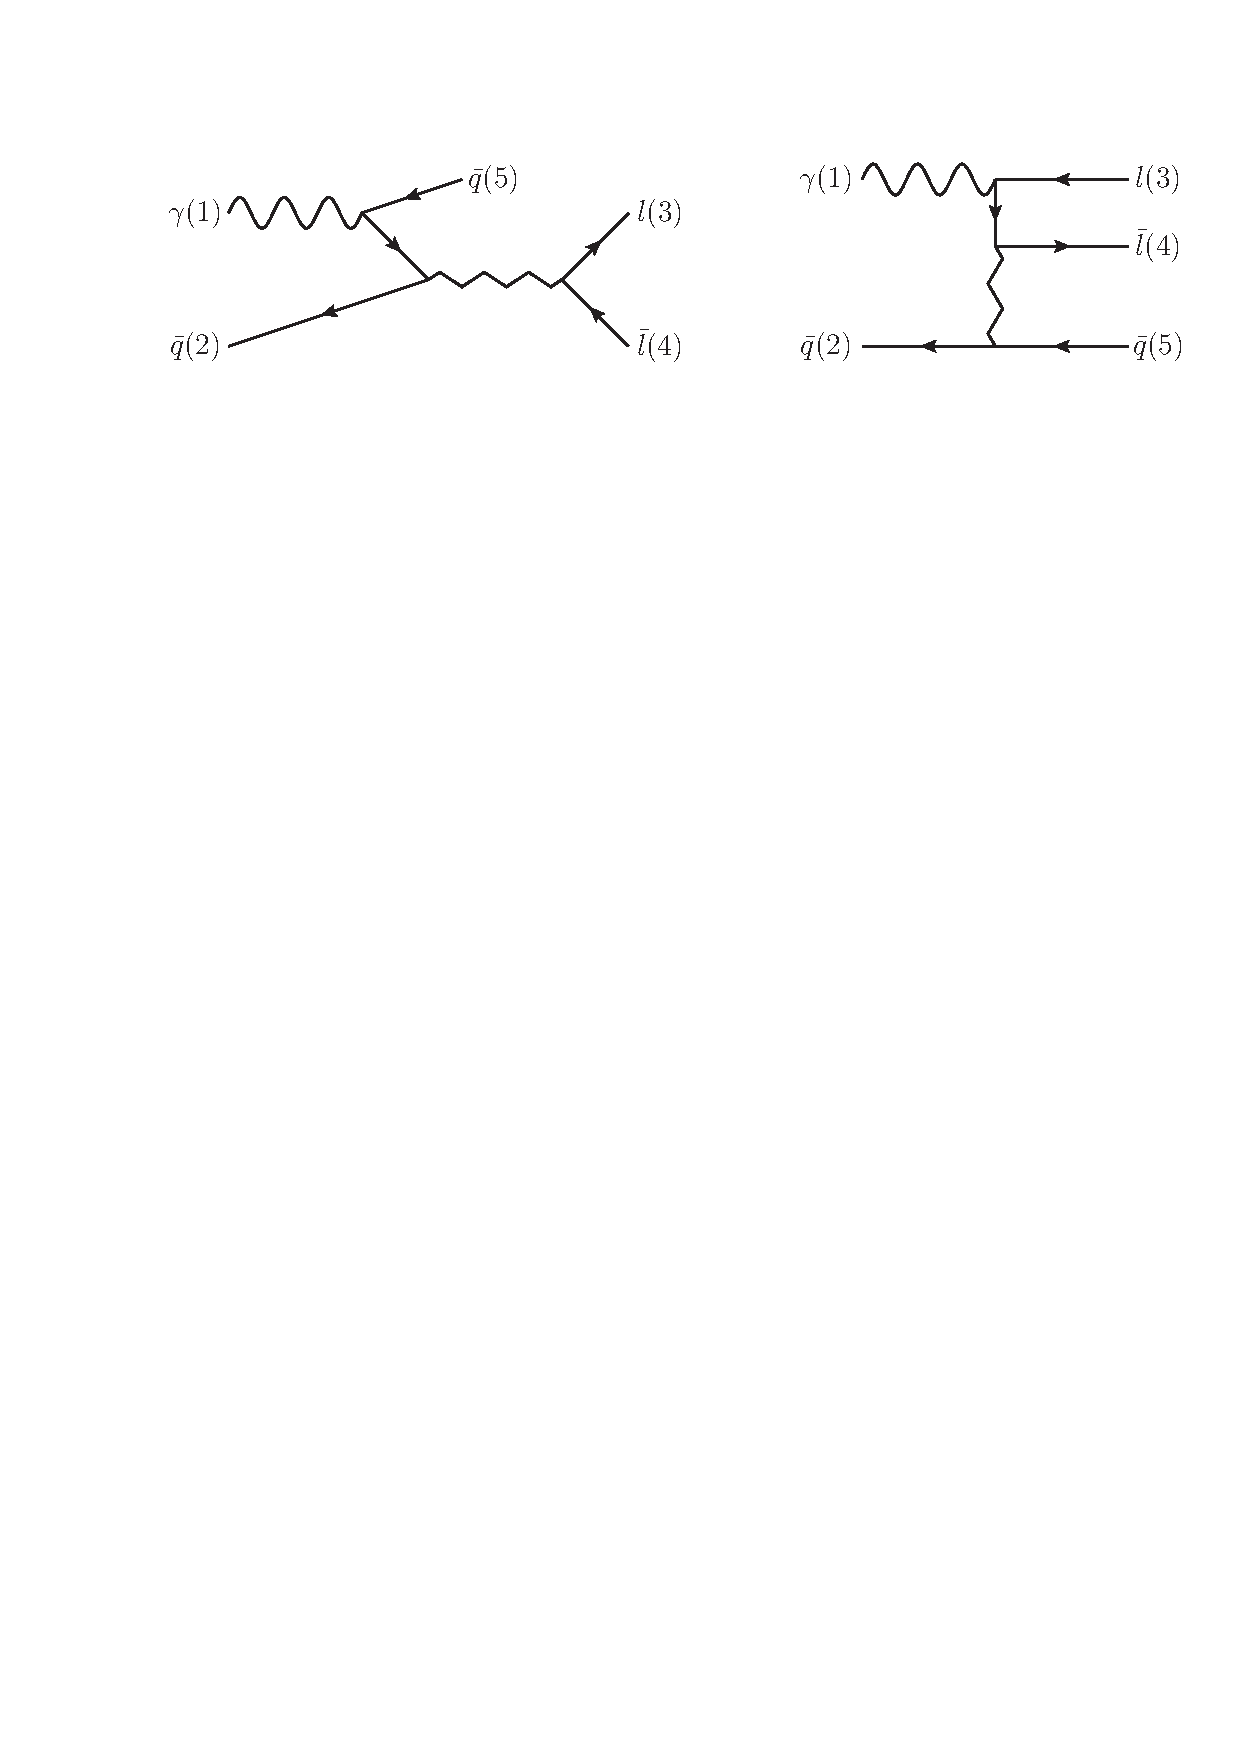
\includegraphics[width=0.7\linewidth]{aq_NLO}
  \caption{sample of Feynman diagrams contributing to the $\gamma \barq \rightarrow e^- \, e^+ \, \barq$ scattering, and representing topology $T_1$ and $T_2$, respectively.}
  \label{fig:aqNLO}
\end{figure}
%%%%%%%%%%%%
 The behaviour of the NLO matrix element corresponding to topology $T_1$ can be deduced from Eq.\eqref{eq:C_51_gq} up to natural modifications. In particular we have
\beq
C_{15} \, F_{LM}(1_\gamma,2_{\bar{q}},3_{e^-},4_{e^+} | 5_{\bar{q}}) = e^2_{b} \, Q_q^2\, N_c  \; \frac{1}{p_1\cdot p_5} \; 
P_{g\bar{q}}(z) \, \frac{F_{LM}(z\cdot 1_{q},2_{\bar{q}},3_{e^-},4_{e^+})}{z} 
 \; ,
 \label{eq:C_15_aq}
\eeq
with $P_{g\bar{q} }(z) =  1- {2z(1-z)}/{(1-\eps)}$, $z = (E_1-E_5)/E_1$, and $N_c$ equal to the number of colors of the theory. The color factor arises because 
the 5-point amplitude appearing on the r.h.s. of Eq.\eqref{eq:C_15_aq} is proportional to
\beq
F_{LM}(1_\gamma,2_{\bar{q}},3_{e^-},4_{e^+} | 5_{\bar{q}}) 
\propto
\underbrace{\frac12 \, \frac12}_{IS \, spin} 
\; \cdot \; 
\underbrace{\frac1{N_c}}_{IS \, color}
\; \cdot \; 
\overbrace{N_c}^{FS \, color}
= \frac14 \, , 
\eeq
while the 4-point amplitude appearing on the l.h.s. gives
\beq
F_{LM}(z\cdot 1_{q},2_{\bar{q}},3_{e^-},4_{e^+})
\propto
\underbrace{\frac12 \, \frac12}_{IS \, spin} 
\; \cdot \; 
\underbrace{\frac1{N_c} \, \frac1{N_c} }_{IS \, color}
\; \cdot \; 
\overbrace{N_c}^{FS \, color} 
= \frac14 \, \frac1{N_c} \, . 
\eeq
The restore the equivalence of the two matrix element (with respect to color factor) it is then necessary to include a $N_c$ factor in the l.h.s.
The integrated counterpart of Eq.\eqref{eq:C_15_aq}, {\it mutatis mutandi}, is given by Eq.\eqref{eq:integrated_collinear_NLO_gq}, namely
\beq
&&
\int [dp_5] C_{51} F_{LM} (1_\gamma,2_{\bar{q}},3_{e^-},4_{e^+} | 5_{\bar{q}}) 
= 
\nn \\
&&  =
-\frac{[\alpha_{b}]}{\eps}\, Q_q^2 \, N_c \, (2E_1)^{-2\eps} \, 
\frac{\Gamma^2(1-\eps)}{\Gamma(1-2\eps)} 
\int_{0}^1 dz \, (1-z)^{-2\eps} 
P_{\barq g} (z) \, 
\Big\langle \frac{F_{LM}(z\cdot 1_{q},2_{\bar{q}},3_{e^-},4_{e^+})}{z} \Big\rangle
\nn \\
&&  =
-\frac{[\alpha_{b}]}{\eps}\, Q_q^2 \, N_c \, (2E_1)^{-2\eps} \, 
\frac{\Gamma^2(1-\eps)}{\Gamma(1-2\eps)} 
\int_{0}^1 dz \, 
P_{\barq g}^{\rm NLO} (z) \, 
\Big\langle \frac{F_{LM}(z\cdot 1_{q},2_{\bar{q}},3_{e^-},4_{e^+})}{z} \Big\rangle ,
\qquad
\label{eq:C51_aq_NLO}
\eeq
where $P_{\barq g}^{\rm NLO} (z)$ is defined in Eq.\eqref{eq:P_barqg_NLO}
 We now focus on topology $T_2$. It is important to stress that under collinear limit $C_{52}$ the hard subprocess is boson-induced and therefore spin-correlations have to be taken into account.
 %%%figure%%%%%%
\begin{figure}
\centering
  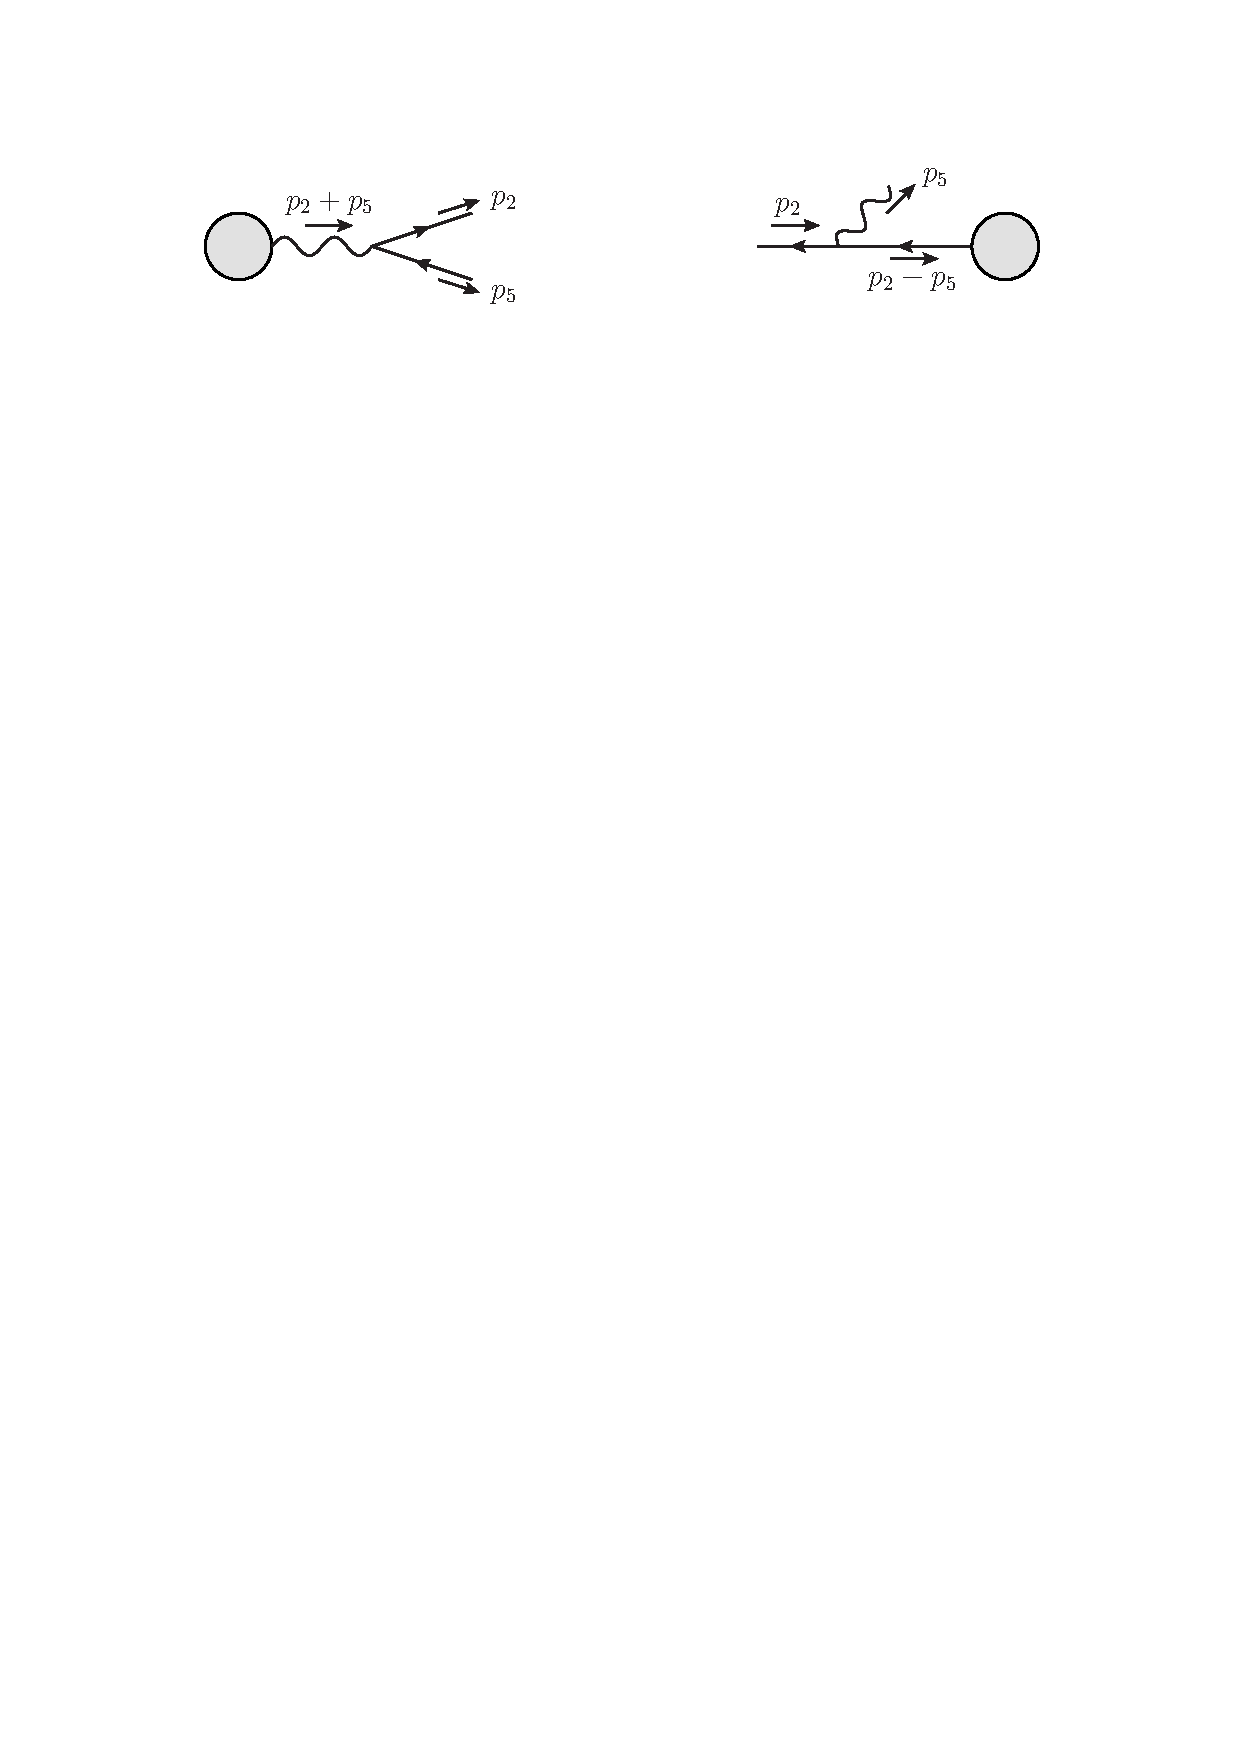
\includegraphics[width=0.7\linewidth]{collinear_temp}
  \caption{Feynman diagrams for initial and final splitting}
  \label{fig:IS-FS_splitting}
\end{figure}
%%%%%%%%%%%%
 The collinear factorisation can be then express as
  \beq
C_{25} \, F_{LM}(1_\gamma,2_{\bar{q}},3_{e^-},4_{e^+} | 5_{\bar{q}}) = e^2_{b} \, Q_q^2\,   \; \frac{1}{p_2\cdot p_5} \; 
P^{\mu \nu}_{q\gamma}(1/z)\,  (1-\eps) \, F_{LM}^{\mu \nu}(1_{\gamma},z\cdot2_{\gamma},3_{e^-},4_{e^+})
 \; ,
 \label{eq:C_25_aq_temp}
\eeq
 \Chiara[check the overall sign!!!!] \\
with $z = (E_2-E_5)/E_2$ and 
\beq
P^{\mu \nu}_{q\gamma}(y) 
=
- g^{\mu \nu} + 4 y (1- y) \frac{k_\bot^\mu \, k_\bot^\nu}{k_\bot^2} \, .
\eeq
 In order to write Eq.\eqref{eq:C_25_aq_temp} one can start from the collinear factorisation in the case of final state splitting, see the right panel in Fig.\ref{fig:IS-FS_splitting},
  \beq
C_{25}^{\rm FSR} \, F_{LM}(2_{\bar{q}}, 5_{\bar{q}}) = e^2_{b} \, Q_q^2\,   \; \frac{1}{p_2\cdot p_5} \; 
P^{\mu \nu}_{q\gamma}(z')\, (1-\eps) \, 
F_{LM}^{\mu \nu}\Big(\frac1{z'}\cdot 2_{\gamma}\Big) \; ,
\qquad \qquad
z' = \frac{E_2}{E_2+E_5} 
 \; .
 \label{eq:C_25_aq_temp2}
\eeq
Then we realise that to cross parton 2 in the initial state we need to reverse its energy, i.e. substitute $E_2 \rightarrow - E_2$ (see the left panel in Fig.\ref{fig:IS-FS_splitting}). As a consequence, we have
\beq
z' \rightarrow \tilde{z} = \frac{-E_2}{-E_2 +E_5} = \frac{E_2}{E_2-E_5} \equiv \frac1z  \, ,
\eeq
 and then
   \beq
C_{25}^{\rm ISR} \, F_{LM}(2_{\bar{q}}, 5_{\bar{q}}) = e^2_{b} \, Q_q^2\,   \; \frac{1}{p_2\cdot p_5} \; 
P^{\mu \nu}_{q\gamma}(1/z)\, 
(1-\eps) \,
F_{LM}^{\mu \nu}\big(z\cdot 2_{\gamma}\big) \; ,
\qquad \qquad
z = \frac{E_2-E_5}{E_2}
 \; ,
 \label{eq:C_25_aq_temp3}
\eeq
consistently with Eq.\eqref{eq:C_25_aq_temp}. \\
 \Chiara[check the overall sign!!!!] \\
At this point we can show that the tree level matrix element appearing in the r.h.s. of the equation above is not spin correlated and thus we can mediate over the polarisation stated of the parent photon. Do to so, we have to compute 
\beq
\langle P^{\mu \nu}_{q\gamma}(1/z)	\rangle 
= \frac{1}{d-2} \, d_{\mu \nu}(p_2-p_5) P^{\mu \nu}_{q\gamma}(1/z) \, , 
\eeq
where
\beq
d^{\mu \nu}(q) = -g^{\mu \nu} + \frac{n^{\mu} \, p^{\nu} + n^{\nu} \, p^{\mu}}{n\cdot q} \; .
\eeq
Given the properties $-g^{\mu \nu} \, d_{\mu \nu}(q) = d-2$ and $k_\bot \cdot n = 0$, we can easily derive
\beq
\langle P^{\mu \nu}_{q\gamma}(1/z)	\rangle 
&=&
 \frac{1}{d-2} \, d_{\mu \nu}(p_2-p_5) P^{\mu \nu}_{q\gamma}(1/z) 
 \nn \\
 &=&
  \frac{1}{d-2} \, d_{\mu \nu}(p_2-p_5)
  \bigg[
  - g^{\mu \nu} + 4 \,  \frac1z \, \Big(1- \frac1z\Big) \frac{k_\bot^\mu \, k_\bot^\nu}{k_\bot^2}
  \bigg]
  \nn \\
  &=&
   \frac{1}{d-2}
   \bigg[
   d-2 
   + 4 \,  \frac1z \, \Big(1- \frac1z\Big) 
   \Big(  -g^{\mu \nu} + \frac{n^{\mu} \, (p_2-p_5)^{\nu} + n^{\nu} \, (p_2-p_5^{\mu}}{n\cdot (p_2-p_5)} 
   \Big)
   \frac{k_\bot^\mu \, k_\bot^\nu}{k_\bot^2}
   \bigg]
   \nn \\
 & = &
   1
   -  \frac{2}{1-\eps} \,  \frac1z \, \Big(1- \frac1z\Big) 
      \nn \\
 & = &
 \frac1{z} \, 
 \frac{1}{1-\eps}
 \bigg[
 \frac{1+(1-z)^2}{z}
-\eps z
   \bigg]
\eeq
This way, we identically rewrite Eq.\eqref{eq:C_25_aq_temp} as 
  \beq
C_{25} \, F_{LM}(1_\gamma,2_{\bar{q}},3_{e^-},4_{e^+} | 5_{\bar{q}}) &=& e^2_{b} \, Q_q^2\,   \; \frac{1}{p_2\cdot p_5} \; 
P^{\mu \nu}_{q\gamma}(1/z)\, 
(1-\eps) \,
F_{LM}^{\mu \nu}(1_{\gamma},z\cdot2_{\gamma},3_{e^-},4_{e^+})
\nn \\
&=&
e^2_{b} \, Q_q^2\,   \; \frac{1}{p_2\cdot p_5} \; 
\langle  P^{\mu \nu}_{q\gamma}(1/z)\rangle \, 
(1-\eps) \,
\, F_{LM}(1_{\gamma},z\cdot2_{\gamma},3_{e^-},4_{e^+})
\nn \\
&\equiv&
 e^2_{b} \, Q_q^2\,   \; \frac{1}{p_2\cdot p_5} \; 
P_{q\gamma}(z) \, 
\frac{F_{LM}(1_{\gamma},z\cdot2_{\gamma},3_{e^-},4_{e^+})}{z} 
 \; ,
 \label{eq:C_25_aq}
\eeq
with 
$z = (E_2-E_5)/E_2$ and 
\beq
P_{q\gamma}(z) = \bigg[
\frac{1+(1-z)^2}{z} -\eps \, z 
\bigg] \, .
\eeq
Let us stress that in this case no color factor has to be added in order to compensate the matrix element reduction. \\
\Chiara[check from here the $1-\eps$ factors] \\
The integrated counterterm is straightforward to compute and reads
\beq
&&\hspace{-20pt}
\big\langle
C_{25} \, F_{LM}(1_\gamma,2_{\bar{q}},3_{e^-},4_{e^+} | 5_{\bar{q}})
\big\rangle =
\int [dp_5] C_{52} F_{LM} (1_\gamma,2_{\bar{q}},3_{e^-},4_{e^+} | 5_{\bar{q}})
\nn \\
&& \quad  =
e^2_{b} \, Q_q^2\,  
\int \frac{d\Omega_5^{(d-1)}}{2 (2\pi)^{d-1}} \frac{1}{\rho_{25}}
\int_0^{E_{\rm max}} \!\! dE_5  \, \frac{ E_5^{1-2\eps}}{E_2 \, E_5} 
P_{q\gamma}(z)  \,
\frac{F_{LM}(1_{\gamma},z\cdot2_{\gamma},3_{e^-},4_{e^+})}{z} 
\nn \\
&&\quad  =
-\frac{[\alpha_{b}]}{\eps}\, Q_q^2 \,   (2E_2)^{-2\eps} \, 
\frac{\Gamma^2(1-\eps)}{\Gamma(1-2\eps)} 
\int_{0}^1 dz \, (1-z)^{-2\eps} 
P_{q\gamma}(z)  \, 
\Big\langle \frac{F_{LM}(1_{\gamma},z\cdot2_{\gamma},3_{e^-},4_{e^+})}{z} \Big\rangle 
\nn \\
&& \quad  =
-\frac{[\alpha_{b}]}{\eps}\, Q_q^2 \,   (2E_2)^{-2\eps} \, 
\frac{\Gamma^2(1-\eps)}{\Gamma(1-2\eps)} 
\int_{0}^1 dz \, 
P_{q\gamma}^{\rm NLO}(z)  \, 
\Big\langle \frac{F_{LM}(1_{\gamma},z\cdot2_{\gamma},3_{e^-},4_{e^+})}{z} \Big\rangle .
\qquad
\label{eq:integrated_collinear_NLO_qgamma}
\eeq
Let us stress that, contrary to the $q\barq$ case, and similarly to the $g\barq$ case, no soft singularities are encoded in the collinear counterterm, since $P_{q\gamma}(z) $ is finite in the $z\rightarrow 1$ limit.
We have defined
\beq
P_{q\gamma}^{\rm NLO}(z) = 
(1-z)^{-2\eps} 
P_{q\gamma}(z)
= {\color{red}{\cancelto{1}{\frac{1}{1-\eps}}}} \, (1-z)^{-2\eps} 
\bigg[
\frac{1+(1-z)^2}{z} -\eps \, z
\bigg] \; .
\eeq
To treat the collinear singularities arising in topology $T_1$ separately with respect to those affecting topology $T_2$ we introduce partition functions
 \beq
\big \langle 
F_{LM}(1_\gamma,2_{\bar{q}},3_{e^-},4_{e^+} | 5_{\bar{q}})
\big \rangle
\equiv
\sum_{i=1}^2
\omega^{5i}
\big \langle 
F_{LM}(1_\gamma,2_{\bar{q}},3_{e^-},4_{e^+} | 5_{\bar{q}})
\big \rangle \, ,
\eeq
where
\beq
1 = \omega^{51} + \omega^{52}
=  \eta_{52} + \eta_{51} \, .
\eeq
Under collinear limit, the partition functions satisfy the following properties
\beq
C_{51} \, \omega^{51} = C_{51}  \, \eta_{52} =  1 \; , 
\qquad
C_{51} \, \omega^{52} = C_{51}  \, \eta_{51} =  0 \; ,
\nn \\
C_{52} \, \omega^{52} = C_{52}  \, \eta_{51} =  1 \; , 
\qquad
C_{52} \, \omega^{51} = C_{52}  \, \eta_{52} =  0 \; .
\eeq
This way we are able to write
\beq
&& \hspace{-25mm}
\big \langle 
F_{LM}(1_\gamma,2_{\bar{q}},3_{e^-},4_{e^+} | 5_{\bar{q}})
\big \rangle
\equiv
\sum_{i=1}^2
\omega^{5i}
\big \langle 
F_{LM}(1_\gamma,2_{\bar{q}},3_{e^-},4_{e^+} | 5_{\bar{q}})
\big \rangle
\nn \\
&=&
\sum_{i=1}^2
\big \langle 
C_{5i} \, 
F_{LM}(1_\gamma,2_{\bar{q}},3_{e^-},4_{e^+} | 5_{\bar{q}})
\big \rangle
+ 
\big \langle 
\mathcal{O}^{\barq}_{\rm nlo} \, 
F_{LM}(1_\gamma,2_{\bar{q}},3_{e^-},4_{e^+} | 5_{\bar{q}})
\big \rangle
\label{eq:partition_NLO_aq}
 \, ,
\eeq
where the fully-regulated term is defined as 
\beq
\mathcal{O}_{\rm nlo}
= 
\sum_{i=1}^2
\mathcal{O}_{\rm nlo}^{(i)}
=
(I- C_{5i}) \, 
\omega^{5i} \; .
\eeq
The collinear pole cancels against the PDFs renormalisation
\beq
2s \cdot d\hat{\sigma}_{{\rm pdf}}
&=&
 2s \cdot d\hat{\sigma}_{{\rm pdf,} T_1}
 +
  2s \cdot d\hat{\sigma}_{{\rm pdf}, T_2}
  \nn \\
 &=&
\frac{\alpha(\mu)}{2\pi \eps} \, 
Q_q^2 \, N_c \,  \int_{0}^{1}dz
 \bar{P}_{\barq g}^{\rm AP, 0} (z) \,
\Big\langle \frac{F_{LM}(z\cdot 1_{q},2_{\bar{q}},3_{e^-},4_{e^+})}{z} \Big\rangle
\nn \\
&&
+ \frac{\alpha(\mu)}{2\pi \eps} \, 
Q_q^2 \,  \int_{0}^{1}dz \, 
 \bar{P}_{q\gamma}^{\rm AP, 0} (z) \,
\Big\langle \frac{F_{LM}(1_{\gamma},z\cdot2_{\gamma},3_{e^-},4_{e^+})}{z} \Big\rangle
\\  \nn 
 &=&
  [\alpha_b]
\frac{Q_q^2 \, N_c }{\eps} \, 
\frac{\Gamma(1-\eps)}{\mu^{2\eps} \, e^{ \eps \gamma_E}}
\int_{0}^{1}dz
 \bar{P}_{\barq g}^{\rm AP, 0} (z) \, 
 \Big\langle \frac{F_{LM}(z\cdot 1_{q},2_{\bar{q}},3_{e^-},4_{e^+})}{z} \Big\rangle 
 \nn \\
 &&
 +
  [\alpha_b]
\frac{Q_q^2}{\eps} \, 
\frac{\Gamma(1-\eps)}{\mu^{2\eps} \, e^{\eps \gamma_E}}
\int_{0}^{1}dz \, 
\bar{P}_{q\gamma}^{\rm AP, 0} (z) \, 
 \Big\langle \frac{F_{LM}(1_{\gamma},z\cdot2_{\gamma},3_{e^-},4_{e^+})}{z} \Big\rangle  \, ,
  \eeq
  where $\bar{P}_{\barq q}^{\rm AP, 0}$ is the color-stripped LO Altarelli-Parisi splitting function, defined as
 \beq
  \bar{P}_{\barq g}^{\rm AP, 0}(z)
  = 
  (1-z)^2+z^2 \, .
  \label{eq:PbarqgAP0}
 \eeq
and  $\bar{P}_{q\gamma}^{\rm AP, 0} (z)$ is given by
 \beq
\bar{P}_{q\gamma}^{\rm AP, 0} (z)
  = 
\frac{1+(1-z)^2}{z} \, .
  \label{eq:PqaAP0}
 \eeq
 

 \subsubsection{Poles cancellation}
We are now in the position to express the full cross-section for the $\gamma \barq$ channel in terms of finite quantities.
 By combining the integrated collinear counterterms and the pdf renormalisation we easily obtain
 \beq
2 s\cdot d\hat{\sigma}_{\rm nlo}^{\gamma \barq}
&=&
2 s\cdot  d\hat{\sigma}_{\rm r}^{\gamma \barq}
+
2 s\cdot  d\hat{\sigma}_{\rm pdf}^{\gamma \barq}
\nn \\
&=&
\big \langle 
\mathcal{O}^{\barq}_{\rm nlo} \, 
F_{LM}(1_\gamma,2_{\bar{q}},3_{e^-},4_{e^+} | 5_{\bar{q}})
\big \rangle 
\nn \\
&&
-\frac{[\alpha_{b}]}{\eps}\, Q_q^2 \, N_c \, (2E_1)^{-2\eps} \, 
\frac{\Gamma^2(1-\eps)}{\Gamma(1-2\eps)} 
\int_{0}^1 dz \, 
P_{\barq g}^{\rm NLO} (z) \, 
\Big\langle \frac{F_{LM}(z\cdot 1_{q},2_{\bar{q}},3_{e^-},4_{e^+})}{z} \Big\rangle
\nn \\
&&
-\frac{[\alpha_{b}]}{\eps}\, Q_q^2 \,   (2E_2)^{-2\eps} \, 
\frac{\Gamma^2(1-\eps)}{\Gamma(1-2\eps)} 
\int_{0}^1 dz \, 
P_{q\gamma}^{\rm NLO}(z)  \, 
\Big\langle \frac{F_{LM}(1_{\gamma},z\cdot2_{\gamma},3_{e^-},4_{e^+})}{z} \Big\rangle 
\nn \\
&&
+[\alpha_b]
\frac{Q_q^2 \, N_c }{\eps} \, 
\frac{\Gamma(1-\eps)}{\mu^{2\eps} \, e^{ \eps \gamma_E}}
\int_{0}^{1}dz
 \bar{P}_{\barq g}^{\rm AP, 0} (z) \, 
 \Big\langle \frac{F_{LM}(z\cdot 1_{q},2_{\bar{q}},3_{e^-},4_{e^+})}{z} \Big\rangle 
 \nn \\
 &&
 +
  [\alpha_b]
\frac{Q_q^2}{\eps} \, 
\frac{\Gamma(1-\eps)}{\mu^{2\eps} \, e^{\eps \gamma_E}}
\int_{0}^{1}dz \, 
\bar{P}_{q\gamma}^{\rm AP, 0} (z) \, 
 \Big\langle \frac{F_{LM}(1_{\gamma},z\cdot2_{\gamma},3_{e^-},4_{e^+})}{z} \Big\rangle
 \nn \\
 &=&
 \big \langle 
\mathcal{O}^{\barq}_{\rm nlo} \, 
F_{LM}(1_\gamma,2_{\bar{q}},3_{e^-},4_{e^+} | 5_{\bar{q}})
\big \rangle 
\nn \\
&&
+
[\alpha_{b}]\, 
Q_q^2 \, N_c \,
\int_{0}^1 dz \, 
P_{\barq g}^{\rm fin}(z, E_1)   \, 
 \Big\langle \frac{F_{LM}(z\cdot 1_{q},2_{\bar{q}},3_{e^-},4_{e^+})}{z} \Big\rangle 
\nn \\
&&
+
  [\alpha_b]
  \, Q_q^2 \,
  \int_{0}^1 dz \, 
 P_{q\gamma}^{\rm fin}(z,E_2)  \Big\langle \frac{F_{LM}(1_{\gamma},z\cdot2_{\gamma},3_{e^-},4_{e^+})}{z} \Big\rangle
 \nn \\
 &=&
 [\alpha_b]Q_q^2 \;
 \bigg\{
 \Big[
 z + 2 \Big( \log(1-z)+\log\Big(\frac{2 E_2}{\mu}\Big)\Big) \bar{P}_{q\gamma}^{\rm AP, 0} (z) 
  \Big] \; 
 \Big\langle \frac{F_{LM}(1_{\gamma},z\cdot2_{\gamma},3_{e^-},4_{e^+})}{z} \Big\rangle
 \nn \\
 &&
 + \,2 N_c \,  \Big[
 z(1-z) + \Big( \log(1-z)+\log\Big(\frac{2 E_1}{\mu}\Big)\Big) \bar{P}_{\barq g}^{\rm AP, 0} (z) 
  \Big] \; 
 \Big\langle \frac{F_{LM}(z\cdot1_q, 2_\barq,3_{e^-},4_{e^+})}{z} \Big\rangle
 \bigg\}
 \nn \\
 && 
 + \,  \big \langle 
\mathcal{O}^{\barq}_{\rm nlo} \, 
F_{LM}(1_\gamma,2_{\bar{q}},3_{e^-},4_{e^+} | 5_{\bar{q}})
\big \rangle 
 +\mathcal{O}(\eps)
 \; ,
\eeq
where the finite splitting function contribution is given by 
\beq
P_{\barq g}^{\rm fin}(z, E)
&=&
-\frac1\eps
\bigg\{
\frac{\Gamma^2(1-\eps)}{\Gamma(1-2\eps)} 
 (2E)^{-2\eps} \, 
P_{\barq g}^{\rm NLO} (z) 
-
\frac{\Gamma(1-\eps)}{\mu^{2\eps} \, e^{ \eps \gamma_E}} \, 
 \bar{P}_{\barq g}^{\rm AP, 0} (z)
  \bigg\} \, ,
  \nn \\
  P_{q\gamma}^{\rm fin}(z,E) 
  &=&
   -\frac{1}{\eps}
\bigg\{
\frac{\Gamma^2(1-\eps)}{\Gamma(1-2\eps)} \, 
 (2E)^{-2\eps} \, 
P_{q\gamma}^{\rm NLO}(z)  
-
\frac{\Gamma(1-\eps)}{\mu^{2\eps} \, e^{\eps \gamma_E}}
\bar{P}_{q\gamma}^{\rm AP, 0} (z) \, 
 \bigg\} \, .
\eeq
 
\subsection{Introduction to the NNLO QCD$\times$QED subtraction for $\gamma\barq$ channel}
 
 Here we present the extraction of the IR singularities relevant for the partonic process 
\beq
\gamma(1) +\bar{q}(2) \rightarrow l(3)+\bar{l}(4) + g(5) + \barq(6) \, ,
\eeq  
which is a representative of the following scatterings
\beq
\gamma(1) +\bar{q}(2) \rightarrow l(3)+\bar{l}(4) + g(5) + \barq(6) \, , 
\qquad
\bar{q}(1) + \gamma(2) \rightarrow l(3)+\bar{l}(4) + g(5) + \barq(6) \, , 
\nn \\
\gamma(1) +{q}(2) \rightarrow l(3)+\bar{l}(4) + g(5) + q(6) \, , 
\qquad
q(1) + \gamma(2) \rightarrow l(3)+\bar{l}(4) + g(5) + q(6) \, , 
\nn
\eeq
{\color{orange}{code info}}: notation is chosen according to what is done for the numerical implementation. \\
The cross section receives contribution from a double real contribution, a real-virtual term and the pdf renormalisation, according to 
\beq
d\hat{\sigma}_{\rm nnlo}^{\gamma \barq \rightarrow e^-e^+g\barq}
=
d\hat{\sigma}^{\gamma \barq \rightarrow e^-e^+g\barq}_{\rm rr}
+d\hat{\sigma}^{\gamma \barq \rightarrow e^-e^+g\barq}_{\rm rv}
+d\hat{\sigma}^{\gamma \barq \rightarrow e^-e^+g\barq}_{\rm pdf} \; ,
\eeq
where the double real term is 
\beq
2s\cdot d\hat{\sigma}_{rr}^{\gamma \barq \rightarrow e^-e^+g\barq} 
\equiv 
\int[dp_5] [dp_6] \, F_{LM}(1_\gamma,2_{\bar{q}},3_{e^-},4_{e^+} | 5_g, 6_{\bar{q}})  
\equiv 
\big\langle F_{LM}(1_\gamma,2_{\bar{q}},3_{e^-},4_{e^+} |5_g, 6_{\bar{q}})\big\rangle \, .
\nn
\eeq
 As usual the subtraction procedure begins with the extraction of the soft poles, which 
 in this case may only arise when the gluon momentum vanishes. We proceed in the 
 standard way
 \beq
 \big\langle F_{LM}(1_\gamma,2_{\bar{q}},3_{e^-},4_{e^+} |5_g, 6_{\bar{q}})\big\rangle
&=&
  \big\langle S_{5} \, F_{LM}(1_\gamma,2_{\bar{q}},3_{e^-},4_{e^+} |5_g, 6_{\bar{q}})\big\rangle
  \nn \\
  && 
  + \, 
    \big\langle \big( I -S_{5}\big) \, F_{LM}(1_\gamma,2_{\bar{q}},3_{e^-},4_{e^+} |5_g, 6_{\bar{q}})\big\rangle \; .
  \label{eq:soft_subtra_aq}
 \eeq
 The soft-regulated term is affected by numerous collinear singularities, 
 whole isolation requires a non trivial phase space partition.
 %%%%%%%%%%%figure%%%%%%%%%%
\begin{figure}
    \centering
    \begin{subfigure}{0.3\textwidth}
    \centering
        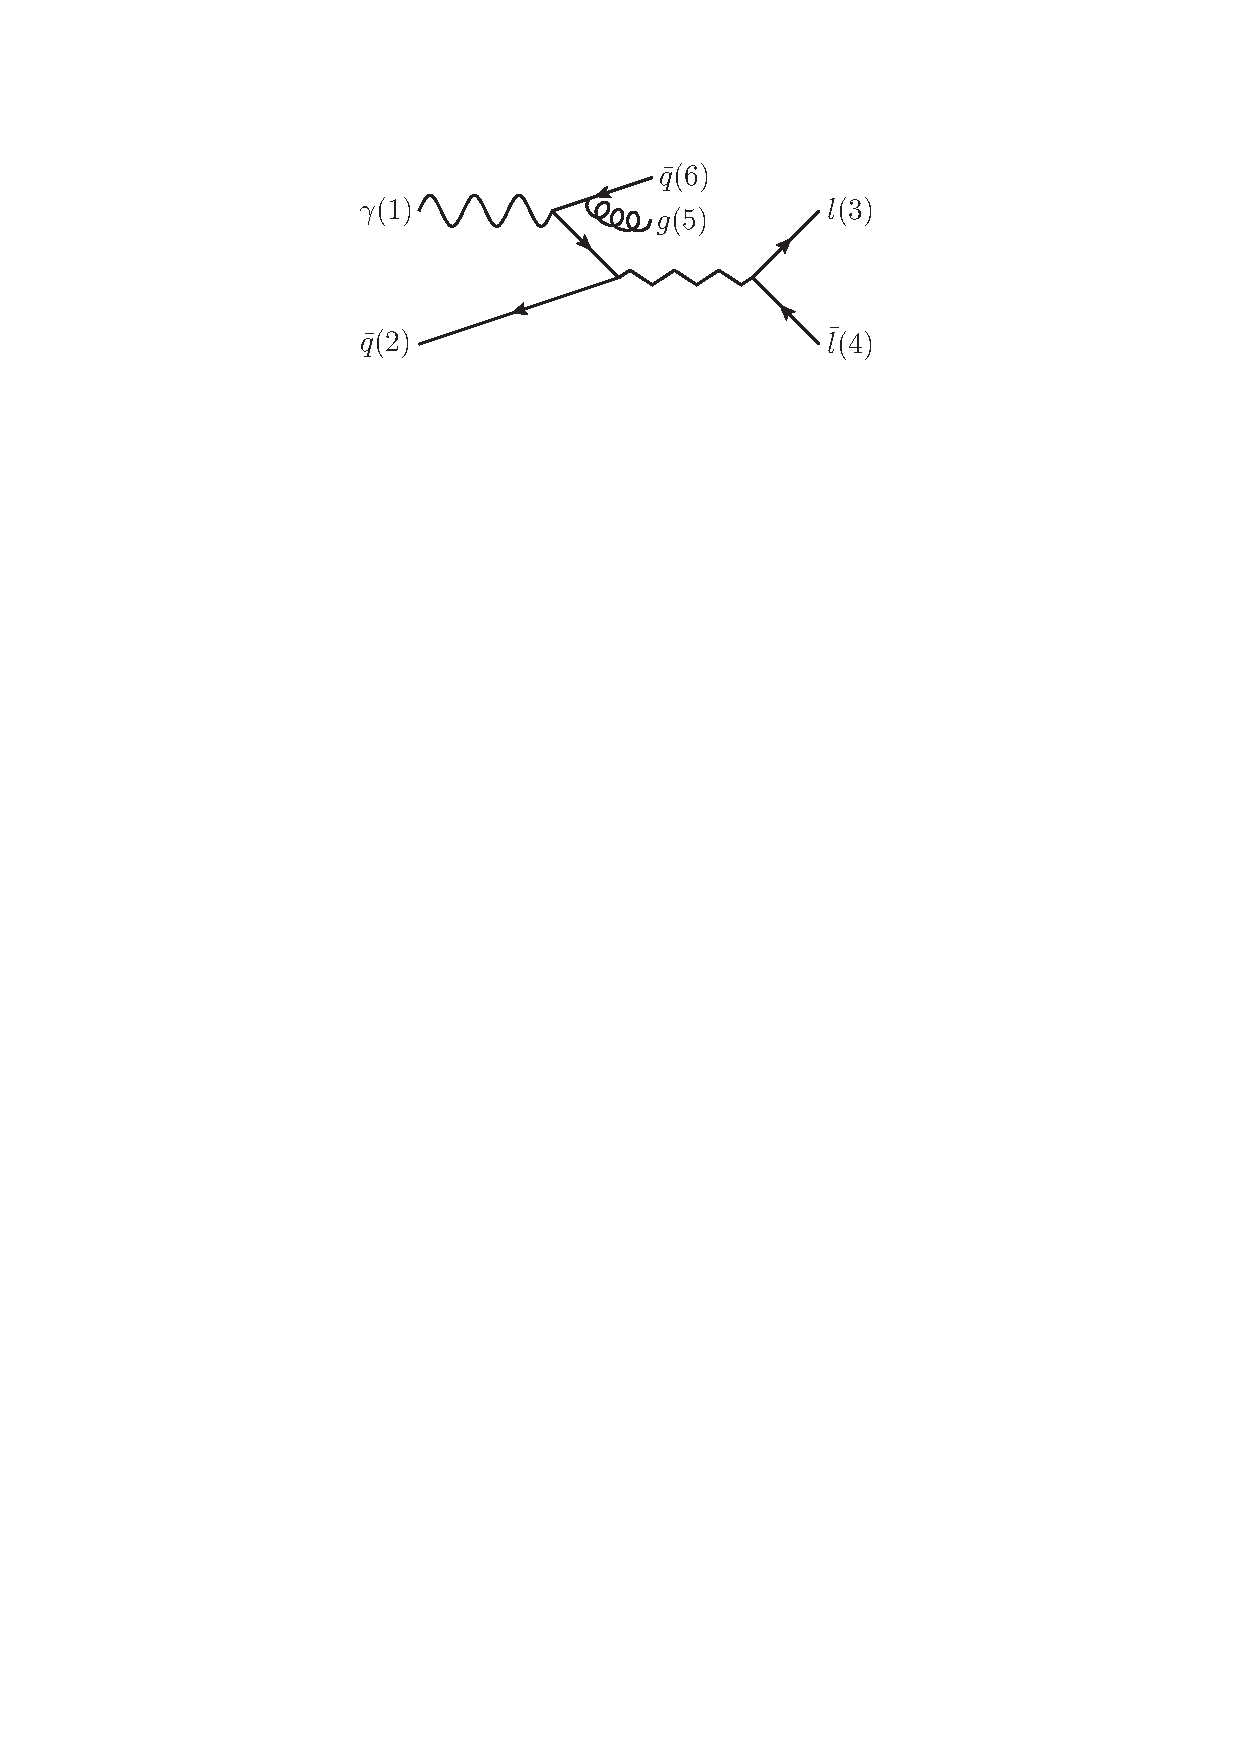
\includegraphics[width=\textwidth]{aq_NNLO_a}
        \caption{}
        \label{fig:LargeOrder_a}
    \end{subfigure}
      \begin{subfigure}{0.3\textwidth}
      \centering
        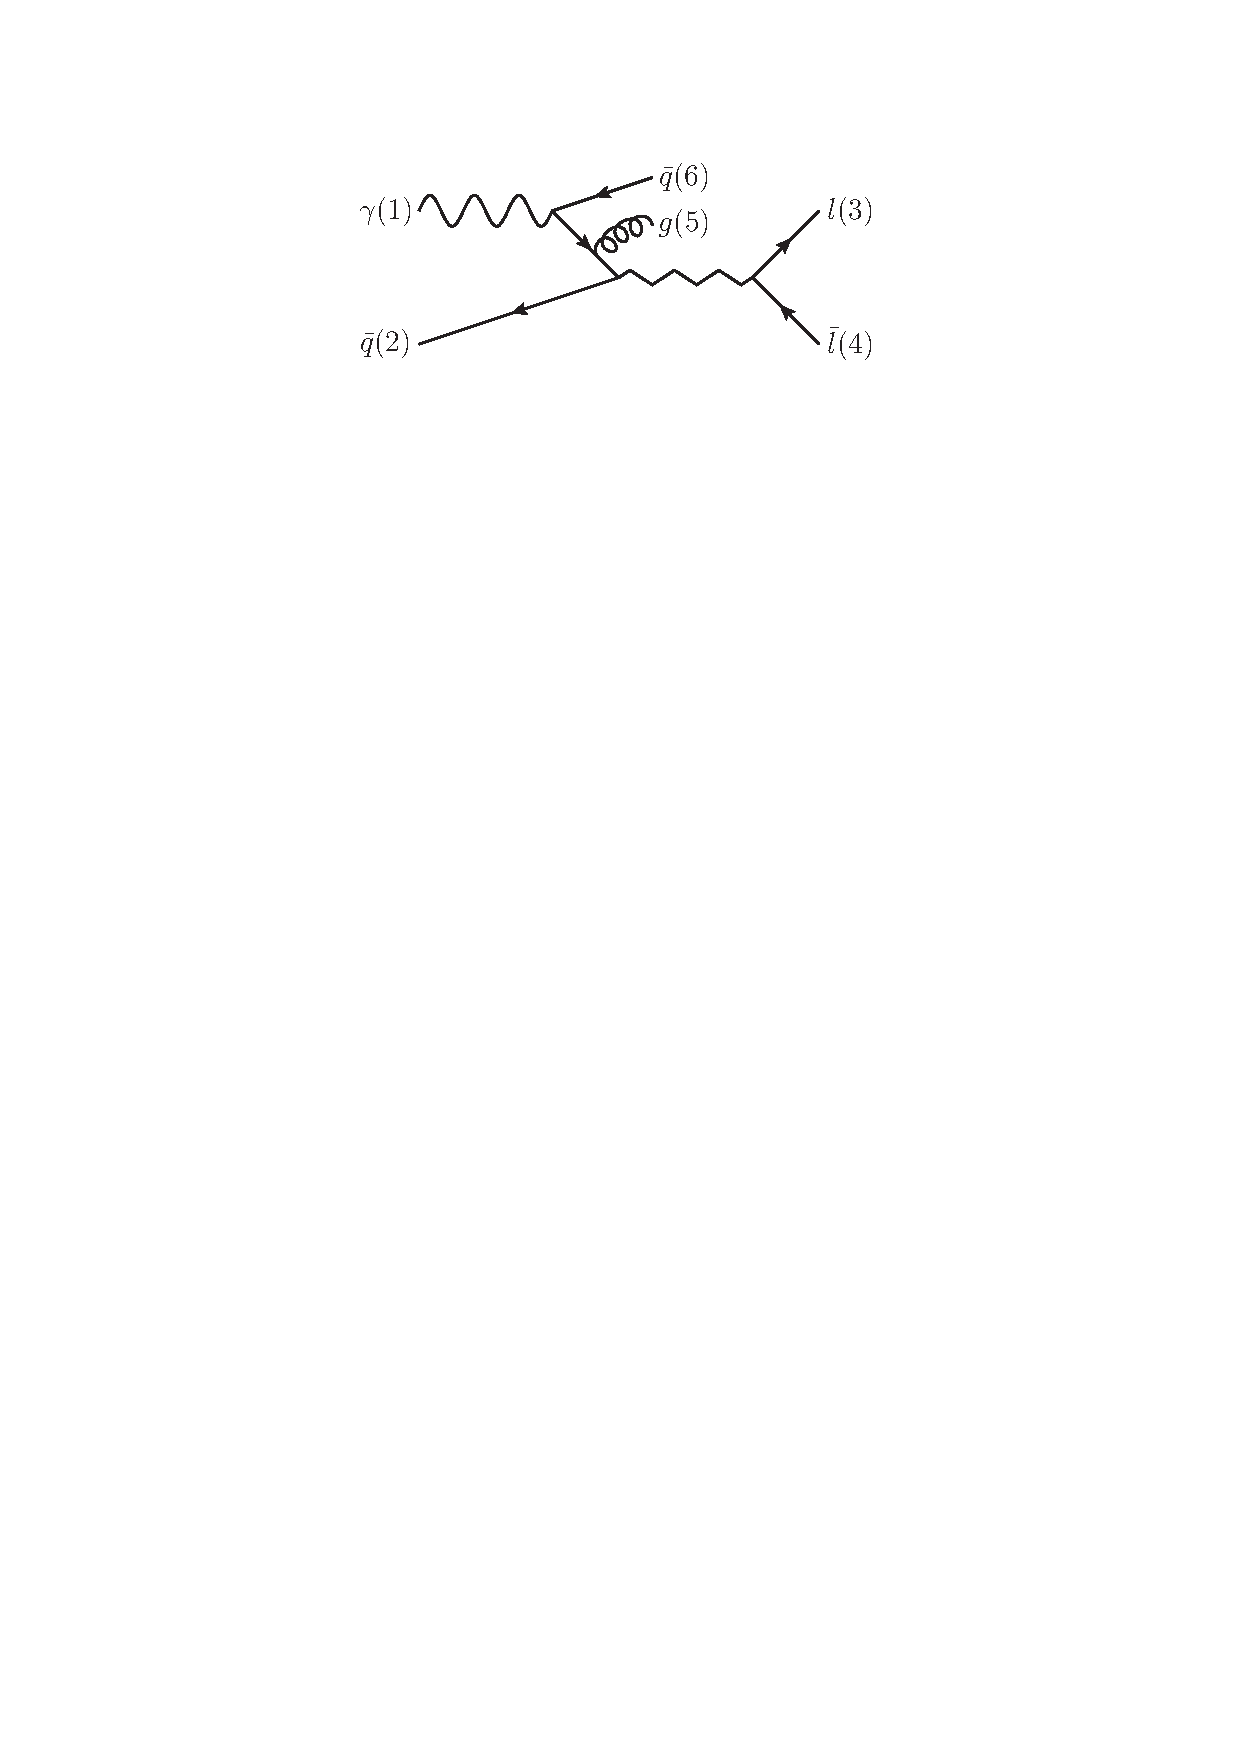
\includegraphics[width=\textwidth]{aq_NNLO_b}
        \caption{}
        \label{fig:LargeOrder_b}
    \end{subfigure}
      \begin{subfigure}{0.3\textwidth}
      \centering
        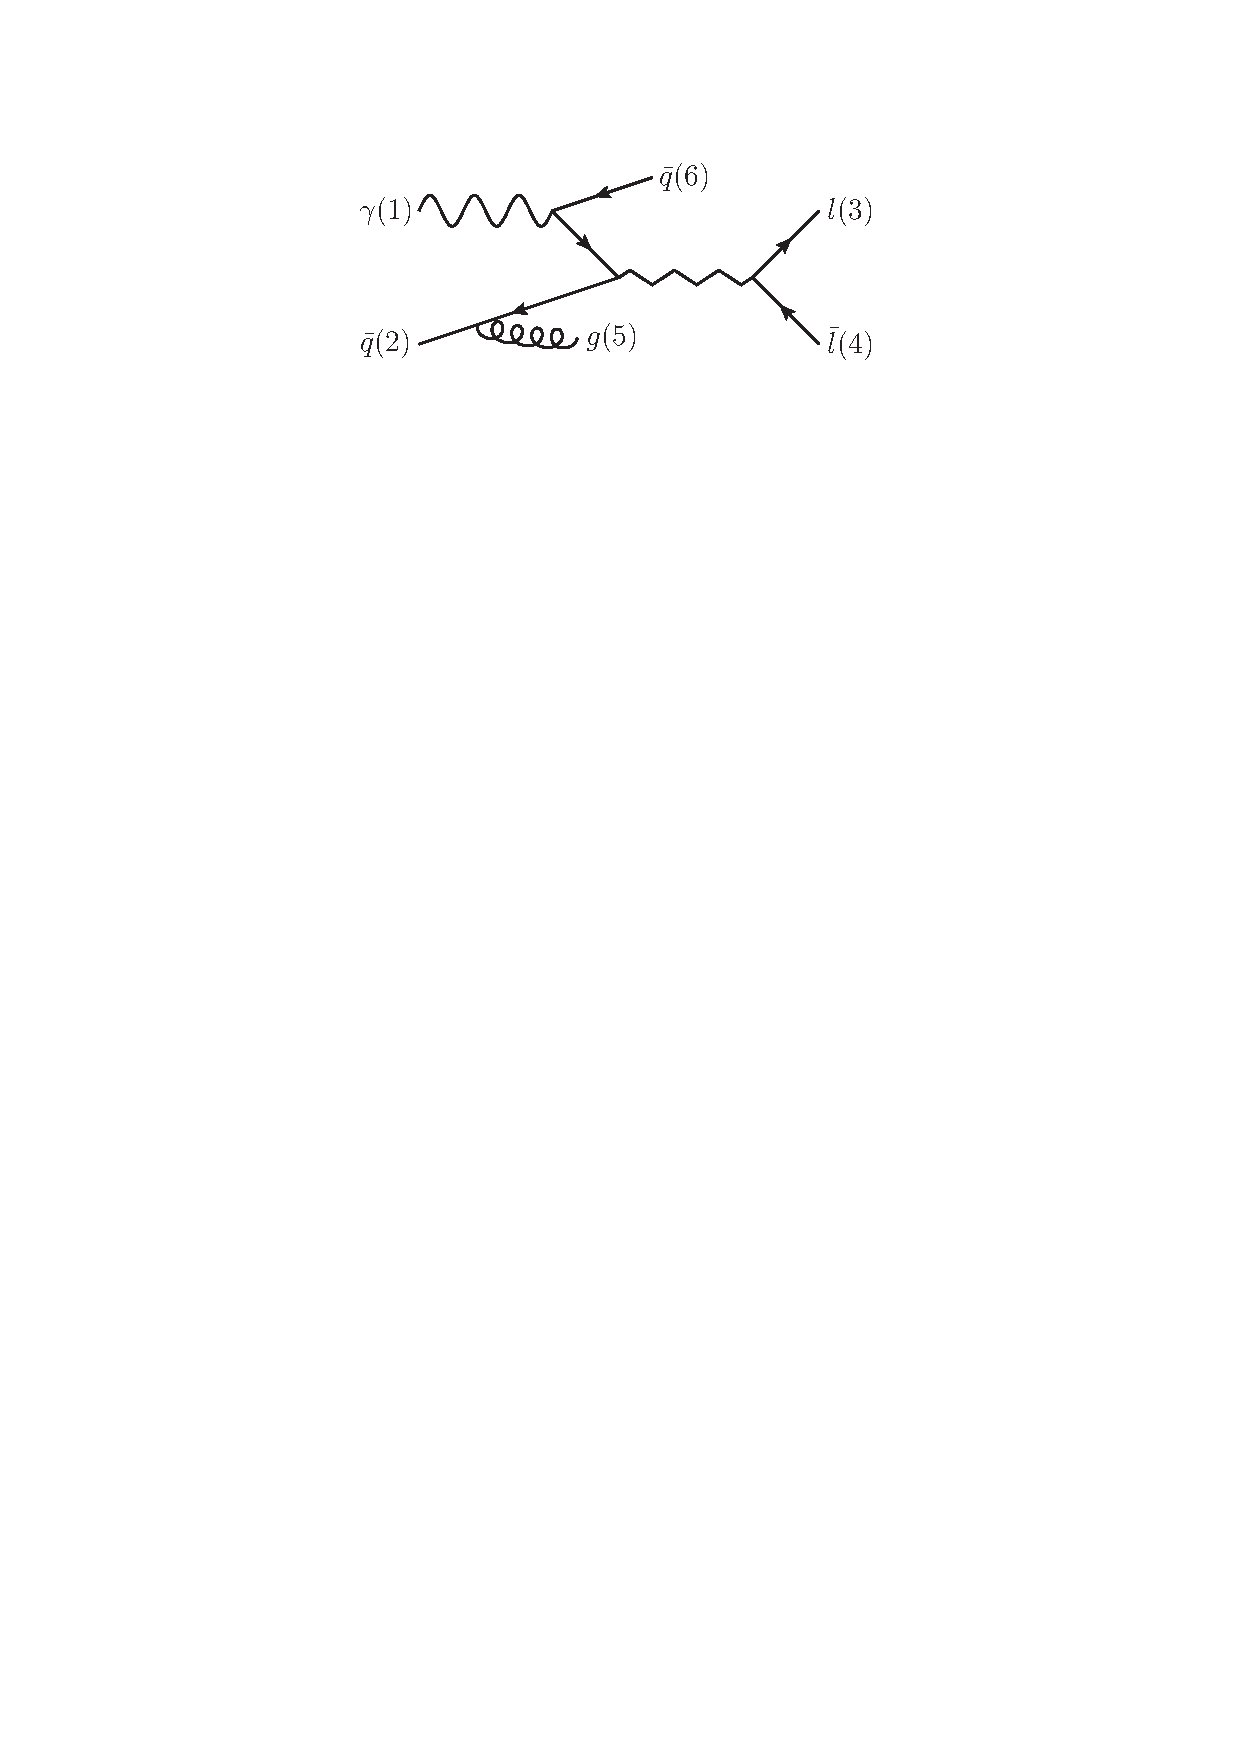
\includegraphics[width=\textwidth]{aq_NNLO_c}
        \caption{}
        \label{fig:LargeOrder_b}
    \end{subfigure}
      \caption{Examples of Feynman graphs contributing to the NNLO correction for the $s$-channel.}
  \label{fig:nnlo_aq}
\end{figure}
%%%%%%%%%%%%%%%%%%%%%%
 %%%%%%%%%%%figure%%%%%%%%%%
\begin{figure}
    \centering
    \begin{subfigure}{0.3\textwidth}
    \centering
        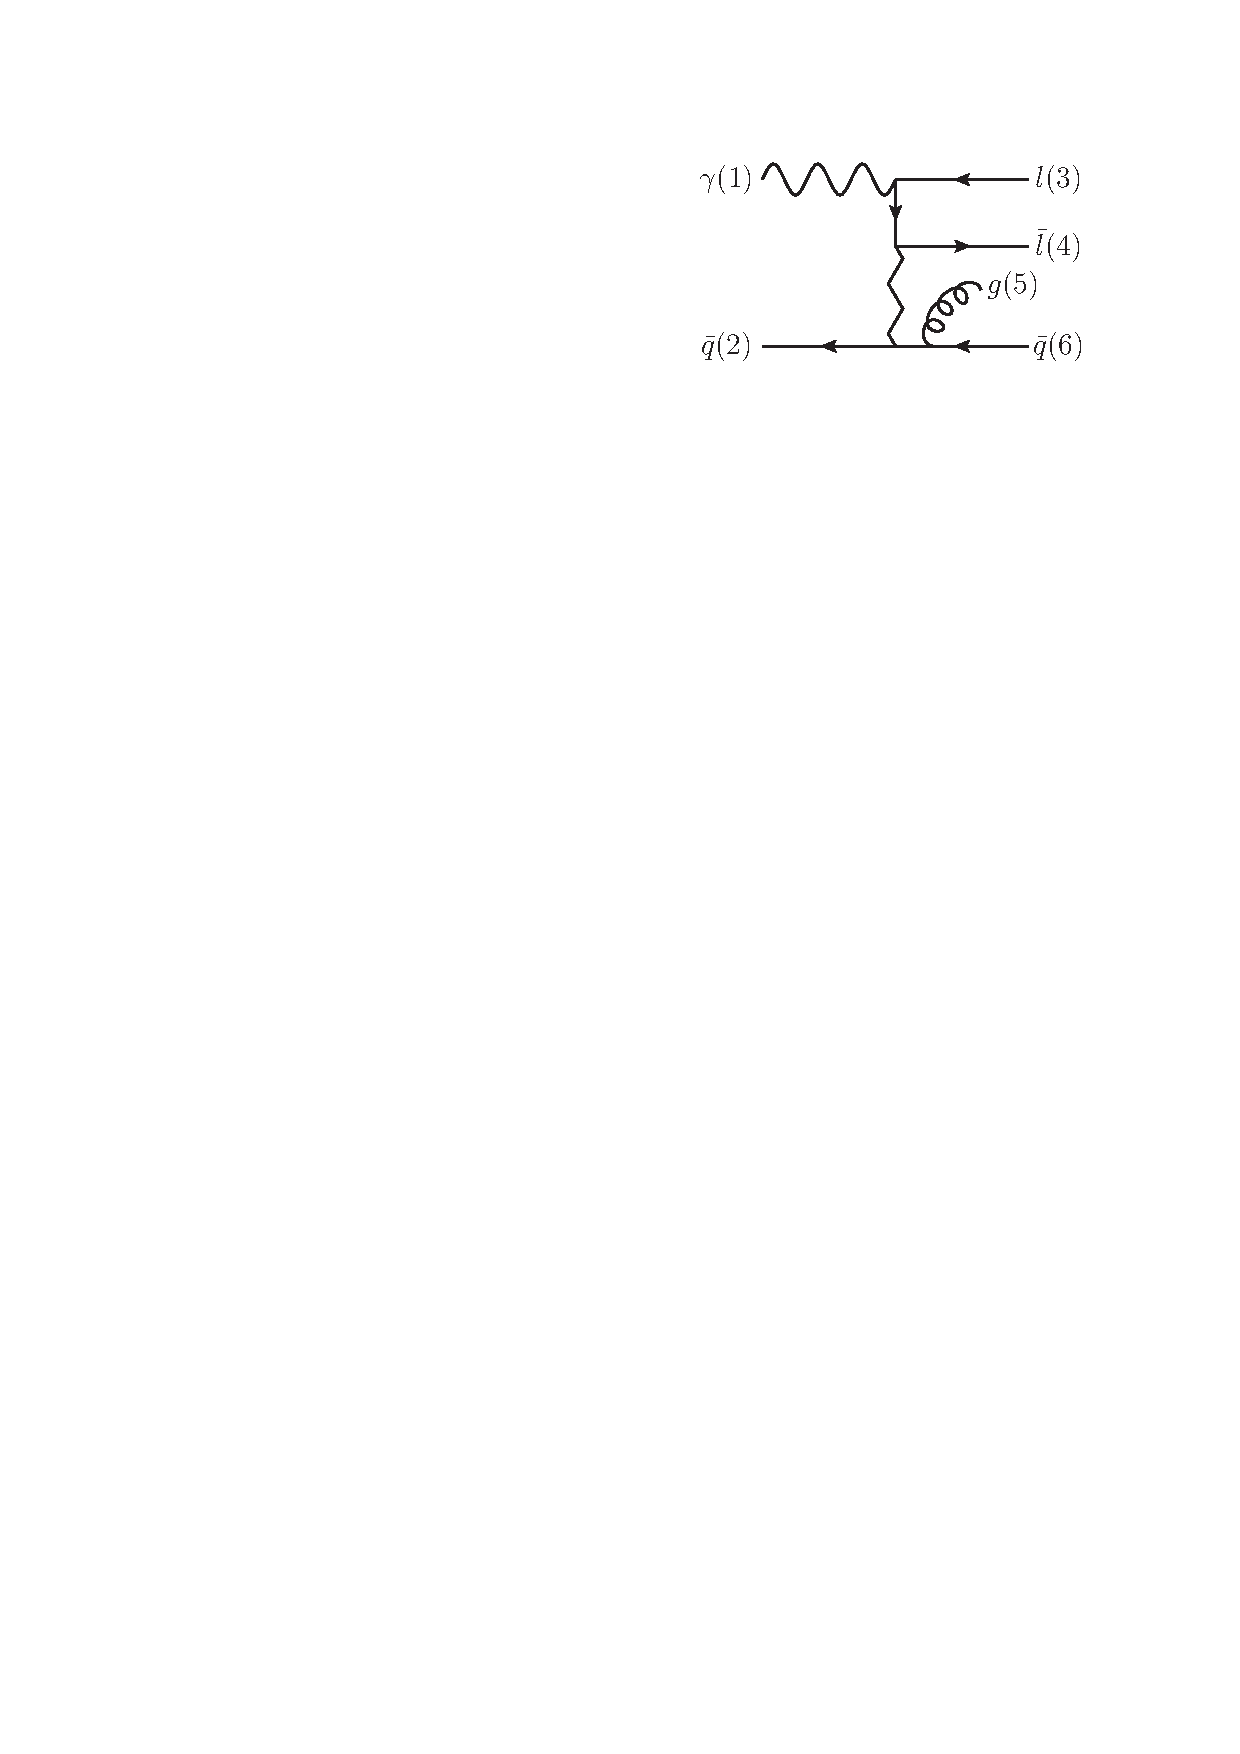
\includegraphics[width=0.8\textwidth]{aq_NNLO_d}
        \caption{}
        \label{fig:LargeOrder_a}
    \end{subfigure}
      \begin{subfigure}{0.3\textwidth}
      \centering
        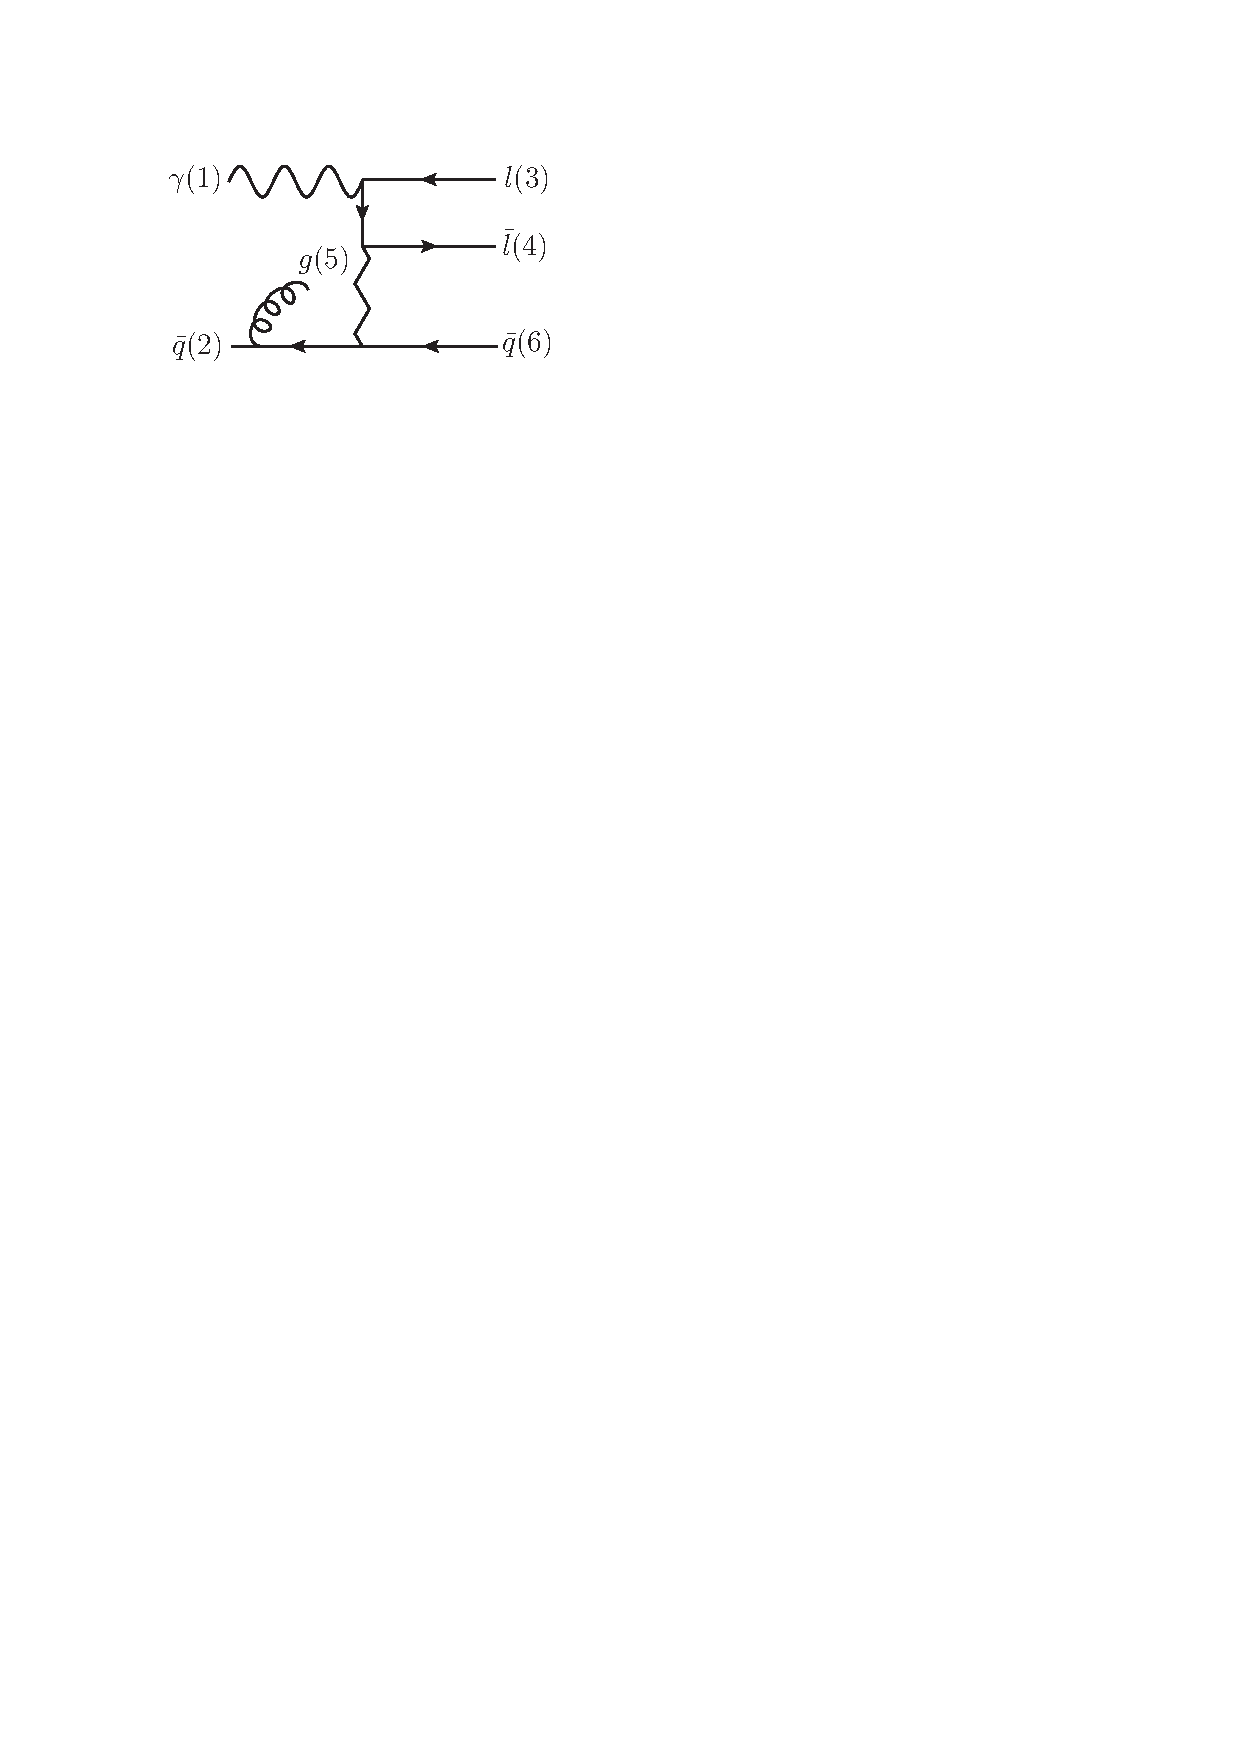
\includegraphics[width=0.8\textwidth]{aq_NNLO_e}
        \caption{}
        \label{fig:LargeOrder_b}
    \end{subfigure}
      \caption{Examples of Feynman graphs contributing to the NNLO correction for the $t$-channel.}
  \label{fig:nnlo_aq}
\end{figure}
%%%%%%%%%%%%%%%%%%%%%%
Among the collinear singularities, we mention the triple collinear divergences arising when the emitted (anti)quark and gluon become collinear to the  photon or to the initial state (anti)quark. Single collinear singularities have also to be considered. In particular we need to take care of the configurations where the gluon is collinear to one of the interactive partons. Guided by the approach adopted to treat color singlet production at NNLO QCD (see Ref.1902.02081 and in particular Eq.3.12) we decide to introduce two {\it triple collinear sectors}, one for each resolved initial state direction, and two {\it double collinear sectors}, whose structure will be discuss in details in the following. In the present subsection we limit ourselves to present the partition function and the corresponding properties.  \\
We begin by enumerating the collinear limits contributing to the process:
\begin{itemize}
\item the gluon is collinear to the outgoing quark, 
\item the gluon is collinear to the incoming quark, 
\item the outgoing quark is collinear to the photon, 
\item the gluon and the outgoing quark are both collinear to the photon, 
\item the overlapping between the previous configurations \, .
\end{itemize}
To maximally reduce the number of collinear singularities to treat at once we introduce the partition
\beq
1 = \omega^{51,61}+ \omega^{52,62} + \omega^{52,61} + \omega^{51,62} \, ,
\label{eq:partition_aq_temp}
\eeq
where the first two sectors contain triple collinear singularities relative to $\gamma(1)$ and $\barq(2)$ respectively, while the third and the forth sectors are responsible for single collinear limits regularisation. Triple collinear sectors requires a further partition to divide strongly-ordered configurations and optimise the phase space parametrisation. 
We then write 
\Chiara[CHECK CONSISTENCY WITH THE PRESENT CASE OF THE NEXT TWO EQUATIONS]
\beq
\omega^{51,61}
\!\!&=&\!\!
\omega^{51,61}
\bigg[
\theta \Big(\rho_{16} < \frac{\rho_{15}}{2} \Big)
+
 \theta \Big(\frac{\rho_{15}}{2}<\rho_{16} < \rho_{15} \Big)
 +
 \theta \Big(\rho_{15} < \frac{\rho_{16}}{2} \Big)
 +
 \theta \Big(\frac{\rho_{16}}{2}<\rho_{15} < \rho_{16} \Big)
 \bigg]
\nn \\
\!\!&=&\!\!
\omega^{51,61}
\Big[
\theta_A
+ \theta_B
+\theta_C
+\theta_D
\Big] \, ,
\eeq
and similarly 
\beq
\omega^{52,62}
\!\!&=&\!\!
\omega^{52,62}
\bigg[
\theta \Big(\rho_{26} < \frac{\rho_{25}}{2} \Big)
+
 \theta \Big(\frac{\rho_{25}}{2}<\rho_{26} < \rho_{25} \Big)
 +
 \theta \Big(\rho_{25} < \frac{\rho_{26}}{2} \Big)
 +
 \theta \Big(\frac{\rho_{26}}{2}<\rho_{25} < \rho_{26} \Big)
 \bigg]
\nn \\
\!\!&=&\!\!
\omega^{52,62}
\Big[
\theta_A
+ \theta_B
+\theta_C
+\theta_D
\Big] \, ,
\eeq
such that Eq.\eqref{eq:partition_aq_temp} can be identically rewritten as 
\beq
1 = \omega^{51,61} \,  \big(
 \theta_A
 + \theta_B
 + \theta_C
 + \theta_D
 \big)
 + \omega^{52,62}  \big(
 \theta_A
 + \theta_B
 + \theta_C
 + \theta_D
 \big)
 + \omega^{52,61} 
 + \omega^{51,62} \, .
\label{eq:partition_aq}
\eeq
In each partition we then have a minimum number of collinear limits. For later convenience we list them below
\beq
\omega^{51,61} \, \theta_A  &:&  C_{61}, \, C_{56, 1}
\nn \\[0.2cm]
&& 
\quad 
\rightarrow \; \omega^{51,61}  \, \theta_A  
=  \big[ C_{61} + C_{56, 1} (1-C_{61}) + (1-C_{56, 1})  (1-C_{61})  \big] \, \omega^{51,61}  \, \theta_A  \; ,
\nn \\[0.3cm]
%%
\omega^{51,61} \, \theta_B  &:& C_{56}, \, C_{56, 1}
\nn \\[0.2cm]
&& 
\quad
\rightarrow \; \omega^{51,61} \, \theta_B 
=\big[ C_{56} + C_{56, 1} (1-C_{56}) + (1-C_{56, 1})  (1-C_{56})  \big] \,  \omega^{51,61} \, \theta_B  \, ,
\nn \\[0.2cm]
%%
\omega^{51,61} \, \theta_C  &:& C_{51}, \, C_{56, 1}
\nn \\[0.2cm]
&& 
\quad
\rightarrow \; \omega^{51,61} \, \theta_C 
=\big[ C_{51} + C_{56, 1} (1-C_{51}) + (1-C_{56, 1})  (1-C_{51})  \big] \,  \omega^{51,61} \, \theta_C  
\nn \\
&& \hspace{27mm}
= \big[ C_{56, 1} + (1-C_{56, 1})  \big] \,  \omega^{51,61} \, \theta_C \, ,
\nn \\[0.2cm]
%%
\omega^{51,61} \, \theta_D  &:& C_{56}, \, C_{56, 1}
\nn \\[0.2cm]
&& 
\quad
\rightarrow \; \omega^{51,61} \, \theta_D 
=\big[ C_{56} + C_{56, 1} (1-C_{56}) + (1-C_{56, 1})  (1-C_{56})  \big] \,  \omega^{51,61} \, \theta_D  \, ,
\nn \\[0.8cm]
%%
\omega^{52,62} \, \theta_A  &:&  C_{62}, \, C_{56,2}
\nn \\[0.2cm]
&& 
\quad 
\rightarrow \; \omega^{52,62}  \, \theta_A  
=  \big[ C_{62} + C_{56, 2} (1-C_{62}) + (1-C_{56,2})  (1-C_{62})  \big] \, \omega^{52,62}  \, \theta_A 
\nn \\
&& \hspace{27mm}
=  \big[ C_{56, 2} + (1-C_{56,2}) \big] \, 
\omega^{52,62}  \, \theta_A 
 \; ,
\nn \\[0.2cm]
%%
\omega^{52,62} \, \theta_B  &:& C_{56}, \, C_{56,2}
\nn \\[0.2cm]
&& 
\quad
\rightarrow \; \omega^{52,62} \, \theta_B 
=\big[ C_{56} + C_{56,2} (1-C_{56}) + (1-C_{56,2})  (1-C_{56})  \big] \,  \omega^{52,62} \, \theta_B 
 \, ,
\nn \\[0.2cm]
%%
\omega^{52,62} \, \theta_C  &:& C_{52}, \, C_{56,2}
\nn \\[0.2cm]
&& 
\quad
\rightarrow \; \omega^{52,62} \, \theta_C 
=\big[ C_{52} + C_{56,2} (1-C_{52}) + (1-C_{56,2})  (1-C_{52})  \big] \,  \omega^{52,62} \, \theta_C  
\nn \\[0.2cm]
%%
\omega^{52,62} \, \theta_D  &:& C_{56}, \, C_{56,2}
\nn \\[0.2cm]
&& 
\quad
\rightarrow \; \omega^{52,62} \, \theta_D 
=\big[ C_{56} + C_{56,2} (1-C_{56}) + (1-C_{56,2})  (1-C_{56})  \big] \,  \omega^{52,62} \, \theta_D  \, ,
\nn \\[0.8cm]
%%
\omega^{51,62} &:& C_{51}, \, C_{62}
\nn \\[0.2cm]
&& 
\quad
\rightarrow \; \omega^{51,62}
= \big[ C_{51} + C_{62} -  C_{62} \, C_{51} + (1-C_{62})  (1-C_{51})  \big] \, 
 \omega^{51,62} 
 \nn \\ 
 && \hspace{22mm}
 =  \big[ C_{62}  + (1-C_{62})   \big] \, \omega^{51,62} 
 \, ,
\nn \\[0.2cm] 
%%
\omega^{52,61} &:& C_{52}, \, C_{61}
\nn \\[0.2cm]
&& 
\quad 
\rightarrow \; \omega^{52,61} =
\big[ C_{52} + C_{61} -  C_{52} \, C_{61} 
+ (1-C_{52})  (1-C_{61}) \big] \, \omega^{52,61}  \; .
\eeq
\Chiara[add comments on simplifications] \\
To simplify the analytic integration of the collinear limits we will not examine one subsector at a time, preferring, instead, to reorganise the counterterms according to their kinematic structure. We consequently introduce a modified partition of the unity 
\beq
1 = \Omega^{\, \gamma \bar{q}} =
\Omega^{\, \gamma\bar{q}}_1
+ \Omega^{\, \gamma\bar{q}}_2
+ \Omega^{\, \gamma\bar{q}}_3
+ \Omega^{\, \gamma\bar{q}}_4    \; , 
\eeq
where the different $\Omega_i^{\; q\bar{q}}$ operators read
\beq
\Omega^{\, \gamma\bar{q}}_1 
&=&
(1-C_{56, 1})  (1-C_{61}) \, \omega^{51,61}  \, \theta_A 
+ 
 (1-C_{56, 1})  (1-C_{56}) \,  \omega^{51,61} \, \theta_B
 \nn \\
 && 
 + \,
 (1-C_{56, 1})   \,  \omega^{51,61} \, \theta_C
 +
  (1-C_{56, 1})  (1-C_{56})  \,  \omega^{51,61} \, \theta_D
  \nn \\
  &&
  + \, 
  (1-C_{56,2})\, \omega^{52,62}  \, \theta_A 
  +
  (1-C_{56,2})  (1-C_{56}) \,  \omega^{52,62} \, \theta_B 
  \nn \\
  && 
  + \, 
  (1-C_{56,2})  (1-C_{52}) \,  \omega^{52,62} \, \theta_C  
  +
  (1-C_{56,2})  (1-C_{56})  \,  \omega^{52,62} \, \theta_D
  \nn \\
  && 
  + (1-C_{62}) \, \omega^{51,62} \; 
  \Chiara[\rightarrow \, \text{ this limit actually do not contribute, 
  see what folows} ]
  \nn \\[10pt]
  %%%%%%%%%%%%%%%%%%%%%%%%%%%%
  \Omega^{\, \gamma\bar{q}}_2
&=&
C_{56, 1} (1-C_{61})  \, 
\omega^{51,61}  \, \theta_A 
+ 
C_{56, 1} (1-C_{56}) \,  \omega^{51,61} \, \theta_B
\nn \\
&& 
+ \, 
 C_{56, 1}  \,  \omega^{51,61} \, \theta_C
+
 C_{56, 1} (1-C_{56})  \,  \omega^{51,61} \, \theta_D 
 \nn \\
 && 
 + \, 
 C_{56,2} \,  \omega^{52,62} \, \theta_A 
 +
C_{56,2} (1-C_{56})  \,  \omega^{52,62} \, \theta_B 
\nn \\
&&
+
 C_{56,2} (1-C_{52}) \,  \omega^{52,62} \, \theta_C
 +
  C_{56,2} (1-C_{56})  \,  \omega^{52,62} \, \theta_D
   \nn \\[10pt]
  %%%%%%%%%%%%%%%%%%%%%%%%%%%%
  \Omega^{\, \gamma\bar{q}}_3
&=&
-  C_{52} \, C_{61}  \, \omega^{52,61}
   \nn \\[10pt]
  %%%%%%%%%%%%%%%%%%%%%%%%%%%%
    \Omega^{\, \gamma\bar{q}}_4
&=&
C_{56}  \,  \big( 
\omega^{51,61} \, \theta_B 
+ 
\omega^{51,61} \, \theta_D
+ 
 \omega^{52,62} \, \theta_B 
 +
 \omega^{52,62} \, \theta_D
 \big)
 \nn \\
 &&
 + \, 
 C_{62}  \, 
 \omega^{51,62} 
 +
 C_{52}  \, \big(  \omega^{52,61} + 
 \omega^{52,62} \, \theta_C   \big)
 +
  C_{61} \, \big(  \omega^{52,61} +
 \omega^{51,61}  \, \theta_A \big)
\eeq
Given this choice of phase space partitioning, we can rewrite the soft-regulated contributions as
\beq
\big\langle \big( I -S_{5}\big) \, F_{LM}(1_\gamma,2_{\bar{q}},3_{e^-},4_{e^+} |5_g, 6_{\bar{q}})\big\rangle
&=& 
\big\langle \big( I -S_{5}\big) \,  \Omega^{\, \gamma \bar{q}} \, F_{LM}(1_\gamma,2_{\bar{q}},3_{e^-},4_{e^+} |5_g, 6_{\bar{q}})\big\rangle
\nn \\
&=&
\sum_{i=1}^4
\big\langle \big( I -S_{5}\big) \,  \Omega^{\, \gamma \bar{q}}_i \, F_{LM}(1_\gamma,2_{\bar{q}},3_{e^-},4_{e^+} |5_g, 6_{\bar{q}})\big\rangle
\; .
\nn 
\eeq
We recall that, as for the channel $q\bar{q}$ channel, all double-collinear operators in $\Omega_i^{\gamma\bar{q}}$ also act on the unresolved phase space, while the triple-collinear operators do not. The physical interpretation of the different $\Omega_i^{\gamma\bar{q}}$ is remarkably simple: $\Omega_1^{\gamma\bar{q}}$ is finite in $d=4$ and can be computed numerically. $\Omega_2^{\gamma\bar{q}}$ contains the contribution of the triple collinear limit, while $\Omega_3^{\gamma\bar{q}}$ encapsulates the double collinear configurations involving two different hard legs. Finally, $\Omega_4^{\gamma\bar{q}}$ describes the various single-collinear subtraction terms. \\


 \subsubsection{Partition functions and their properties}
The explicit expression for the partition functions follows from Eq.3.12 in Ref.1902.02081 and is given by
\beq
\omega^{51,61} &=& \eta_{52} \, \eta_{62} \, \bigg( 
1
+ \frac{\eta_{51}}{\eta_{56}+\eta_{52}+\eta_{61}}
+ \frac{\eta_{61}}{\eta_{56}+\eta_{51}+\eta_{62}}
\bigg) \;  ,
\\ 
\omega^{52,62} &=& \eta_{51} \, \eta_{61} \, \bigg( 
1
+ \frac{\eta_{52}}{\eta_{56}+\eta_{51}+\eta_{62}}
+ \frac{\eta_{62}}{\eta_{56}+\eta_{52}+\eta_{61}}
\bigg) \; ,
\\ 
\omega^{51,62} &=& 
 \frac{\eta_{52} \, \eta_{61} \, \eta_{56}}{\eta_{56}+\eta_{51}+\eta_{62}} \; , 
 \\ 
\omega^{52,61} &=& 
 \frac{\eta_{51} \, \eta_{62} \, \eta_{56}}{\eta_{56}+\eta_{52}+\eta_{61}} \; .
 \label{eq:partition_explicit_aq}
\eeq
Such a functions are designed to verify some crucial properties. In order
\beq
C_{51} \,  \omega^{51,61}  
 \!\!\!&=&\!\!\!
 C_{51} \, 
  \frac{(1+\eta_{56}) \, \eta_{62} } {\eta_{56}+\eta_{62}} 
  \equiv
  \frac{1+\eta_{62}}{2} \, 
C_{51} \,  \equiv \,  
 \tilde{\omega}^{51,61}_{5 \parallel 1} \;  C_{51}
  \;
 \overset{C_{61}}{\longrightarrow}
 \;
 C_{61}
 C_{51}
 \; ,
\label{eq:sector_coll_limit_5161_51}
\\[3pt]
C_{61} \,  \omega^{51,61}  
 \!\!\!&=&\!\!\!
 C_{61} \, 
  \frac{(1+\eta_{56}) \, \eta_{52} } {\eta_{56}+\eta_{52}} 
  \equiv
  (1+\eta_{51}) \, \eta_{52} \, 
C_{61} \,  \equiv \,  
 \tilde{\omega}^{51,61}_{6 \parallel 1} \;  C_{61}
  \;
 \overset{C_{51}}{\longrightarrow}
 \;
 C_{61}
 C_{51}
 \; ,
 \label{eq:sector_coll_limit_5161_61}
\\[3pt]
C_{561} \,  \omega^{51,61}  
 \!\!\!&=&\!\!\!
 C_{561} \, 
 \; ,
\label{eq:sector_coll_limit_5161_561}
\\[3pt]
C_{52} \,  \omega^{52,62}  
 \!\!\!&=&\!\!\!
 C_{52} \, 
  \frac{(1+\eta_{56}) \, (1-\eta_{62}) } {1+\eta_{56}-\eta_{62}} 
  \equiv
  (1-\eta^2_{62}) \, 
C_{52} \,  \equiv \,  
 \tilde{\omega}^{52,62}_{5 \parallel 2} \;  C_{52}
  \;
 \overset{C_{62}}{\longrightarrow}
 \;
 C_{62}
 C_{52}
 \; ,
 \qquad 
\label{eq:sector_coll_limit_5262_52}
\\[3pt]
C_{62} \,  \omega^{52,62}  
 \!\!\!&=&\!\!\!
 C_{62} \, 
  \frac{(1+\eta_{56}) \, (1-\eta_{52}) } {1+\eta_{56}-\eta_{52}} 
  \equiv
  (1-\eta^2_{52}) \,
C_{62} \,  \equiv \,  
 \tilde{\omega}^{52,62}_{6 \parallel 2} \;  C_{62}
  \;
 \overset{C_{52}}{\longrightarrow}
 \;
 C_{62}
 C_{52}
 \; ,
 \label{eq:sector_coll_limit_5262_62}
\\[3pt]
C_{562} \,  \omega^{52,62}  
 \!\!\!&=&\!\!\!
 C_{562} \, 
 \; ,
\label{eq:sector_coll_limit_5262_562}
\\[3pt]
C_{51} \,  \omega^{51,62}  
 \!\!\!&=&\!\!\!
 C_{51} \, 
  \frac{(1-\eta_{62}) \, \eta_{56} } {\eta_{56}+\eta_{62}} 
  \equiv
(1-\eta_{62})^2 \, 
C_{51} \,  \equiv \,  
 \tilde{\omega}^{51,62}_{5 \parallel 1} \;  C_{51}
  \;
 \overset{C_{62}}{\longrightarrow}
 \;
 C_{62}
 C_{51}
 \; , 
 \label{eq:sector_coll_limit_5162_51}
 \\[3pt]
C_{62} \,  \omega^{51,62}  
 \!\!\!&=&\!\!\!
 C_{62} \, 
  \frac{\eta_{52}\, \eta_{56} } {1-\eta_{52}+\eta_{56}} 
  \equiv
\eta_{52}^2 \, 
C_{62} 
\,  \equiv \,  
 \tilde{\omega}^{51,62}_{6 \parallel 2} \;  C_{62}
  \;
 \overset{C_{51}}{\longrightarrow}
 \;
 C_{62}
 C_{51}
 \; , 
 \label{eq:sector_coll_limit_5162_62}
 \\[3pt]
C_{62} \, C_{51} \omega^{51,62}  
 \!\!\!&=&\!\!\!
 C_{51} \, C_{62} \omega^{51,62}  
  = 
 C_{62}
 C_{51}
   = 
 C_{51}
 C_{62}
 \; , 
 \label{eq:sector_coll_limit_5162_5162}
\\[3pt]
C_{52} \,  \omega^{52,61}  
 \!\!\!&=&\!\!\!
C_{52} \,   \frac{\eta_{56} \, \eta_{62}}{1+\eta_{56}-\eta_{62}} \, 
\equiv 
\eta_{62}^2 \, 
 C_{52}
 \equiv \,  
 \tilde{\omega}^{52,61}_{5 \parallel 2} \;  C_{52}
  \;
 \overset{C_{61}}{\longrightarrow}
 \;
 C_{61}
 C_{52}
 \; , 
 \label{eq:sector_coll_limit_5162_51}
 \\[3pt]
C_{61} \,  \omega^{52,61}  
 \!\!\!&=&\!\!\!
 C_{61} \, 
  \frac{\eta_{56}\,(1- \eta_{52}) } {\eta_{52}+\eta_{56}} 
  \equiv
(1-\eta_{52})^2 \, 
C_{61} \,  \equiv \,  
 \tilde{\omega}^{52,61}_{6 \parallel 1} \;  C_{61}
  \;
 \overset{C_{52}}{\longrightarrow}
 \;
 C_{61}
 C_{52}
 \; , 
 \label{eq:sector_coll_limit_5261_61}
 \\[3pt]
C_{52} \, C_{61} \omega^{52,61}  
 \!\!\!&=&\!\!\!
 C_{61} \, C_{52} \omega^{52,61}  
  = 
 C_{52}
 C_{61}
   = 
 C_{61}
 C_{52}
 \; .
 \label{eq:sector_coll_limit_5261_5261}
\eeq

 \paragraph{Sum rules for partition functions}
 Here we report the combinations of sector functions (under specific limits)
 that return the identity. Such considerations are useful for proving the
 poles cancellation (it is important to stress that the poles must cancel 
 independently of the explicit form of the sector functions. However, the partition
 choice determines the weight of the limits and therefore impacts on the 
 functional dependence of the poles coefficients on the process kinematics.
 A change in the partition implies different poles coefficients, but not a spoil 
 of the subtraction.)
 We then have the following relations
\beq
\tilde{\omega}^{51,61}_{5 \parallel 6}
  +
\tilde{\omega}^{52,62}_{5 \parallel 6}
=
1
\, ,
\qquad
\tilde{\omega}^{52,61}_{5 \parallel 2}
  +
\tilde{\omega}^{52,62}_{5 \parallel 2}
=
1 \, , 
\qquad
\tilde{\omega}^{51,61}_{6 \parallel 1}
  +
\tilde{\omega}^{52,61}_{6 \parallel 1}
= 
1 \, 
\nn \\
\tilde{\omega}^{51,61}_{5 \parallel 1}
  +
\tilde{\omega}^{51,62}_{5 \parallel 1}
=
1 \, 
\qquad
\tilde{\omega}^{52,62}_{6 \parallel 2}
  +
\tilde{\omega}^{51,62}_{6 \parallel 2}
=
1
\eeq





\subsection{Real contribution}
In this subsection we analyse the double-real singularities, integrating the relevant counterterms.

\subsubsection{Single soft}

As for the $g \barq$ channel, only one soft-singular regime arises, and it correspond to the first term in Eq.\eqref{eq:soft_subtra_aq}, namely
 \beq
S_{5} \, F_{LM}(1_\gamma,2_{\bar{q}},3_{e^-},4_{e^+} |5_g, 6_{\bar{q}})
 = -  g_{s,b}^2 \sum_{\substack{i,j= \{2, 6\}}}
2 \,  \frac{s_{ij}}{s_{i5} \,s_{j5}} \, \big| M^{{\rm tree}, \, (i,j)}(1_\gamma,2_{\bar{q}},3_{e^-},4_{e^+} | 6_{\bar{q}})\big|^2 \; ,
\eeq
where we have introduced the notation
\beq
  \big| M^{{\rm tree}, \, (i,j)}(1_\gamma,2_{\bar{q}},3_{e^-},4_{e^+} | 6_{\bar{q}})\big|^2 
 \equiv
 \bra{M^{{\rm tree}}(1_\gamma,2_{\bar{q}},3_{e^-},4_{e^+} | 6_{\bar{q}})}{\bf T}_i \cdot {\bf T}_j
\ket{M^{{\rm tree}}(1_\gamma,2_{\bar{q}},3_{e^-},4_{e^+} | 6_{\bar{q}})} \, ,
\eeq
with ${\bf T}_a$ being the standard Catani's color operators.
By exploiting color conservation 
\beq
{\bf T}_2 + {\bf T}_6  =0
\qquad 
{\bf T}_2^2 = {\bf T}_6^2  = C_{F} \; , 
\qquad 
{\bf T}_2 \cdot {\bf T}_6 = {\bf T}_6 \cdot {\bf T}_2 \; ,
\eeq
we obtain
\beq
S_{5} \, F_{LM}(1_\gamma,2_{\bar{q}},3_{e^-},4_{e^+} |5_g, 6_{\bar{q}})
=
 2 C_F \,  g_{s,b}^2 \,  
 \frac{\rho_{26}}{E_5^2 \, \rho_{25}\,  \rho_{56}} \, 
 \, F_{LM}(1_\gamma,2_{\bar{q}},3_{e^-},4_{e^+} | 6_{\bar{q}}) \; .
 \eeq
 
 
 {\color{blue}{
 \beq
 C_{25} \, S_{5} \, F_{LM}(1_\gamma,2_{\bar{q}},3_{e^-},4_{e^+} |5_g, 6_{\bar{q}})
&=&
 2 C_F \,  g_{s,b}^2 \,  
 \frac{1}{E_5^2 \, \rho_{25}\,} \, 
 \, F_{LM}(1_\gamma,2_{\bar{q}},3_{e^-},4_{e^+} | 6_{\bar{q}})
 \nn \\
 \big\langle
  C_{25} \, S_{5} \, F_{LM}(1_\gamma,2_{\bar{q}},3_{e^-},4_{e^+} |5_g, 6_{\bar{q}})
   \big\rangle
&=&
 2 C_F \,  [\alpha_{s,b}]\,  
 \frac{1}{2 \eps^2} \, (2E_{\rm max})^{-2\eps}
 \frac{\Gamma^2(1-\eps)}{\Gamma(1-2\eps)}
 \, F_{LM}(1_\gamma,2_{\bar{q}},3_{e^-},4_{e^+} | 6_{\bar{q}})
 \nn \\
  C_{56} \, S_{5} \, F_{LM}(1_\gamma,2_{\bar{q}},3_{e^-},4_{e^+} |5_g, 6_{\bar{q}})
&=&
 2 C_F \,  g_{s,b}^2 \,  
 \frac{1}{E_5^2 \, \rho_{56}\,} \, 
 \, F_{LM}(1_\gamma,2_{\bar{q}},3_{e^-},4_{e^+} | 6_{\bar{q}})
  \nn \\
 \big\langle
  C_{56} \, S_{5} \, F_{LM}(1_\gamma,2_{\bar{q}},3_{e^-},4_{e^+} |5_g, 6_{\bar{q}})
   \big\rangle
&=&
 2 C_F \,  [\alpha_{s,b}]\,  
 \frac{1}{2 \eps^2} \, (2E_{\rm max})^{-2\eps}
 \frac{\Gamma^2(1-\eps)}{\Gamma(1-2\eps)}
 \, F_{LM}(1_\gamma,2_{\bar{q}},3_{e^-},4_{e^+} | 6_{\bar{q}})
 \nn
 \eeq
 }}
Let us stress that this expression is analogous (up to a minus sign and a invariants relabelling) to the NLO QCD correction to the $q\barq$ channel (see Eq.\eqref{eq:soft_limit_NLO_QCD_qqbar}). The integrated counterterm can be then red directly from (minus) Eq.\eqref{eq:INT_soft_limit_NLO_QCD_qqbar}
\beq
&&\big\langle S_{5} \, F_{LM}(1_\gamma,2_{\bar{q}},3_{e^-},4_{e^+} |5_g, 6_{\bar{q}})\big\rangle 
=
\nn \\
&& \qquad = 
2 C_F \frac{[\alpha_{s,b}]}{\eps^2} 
(2 E_{\rm max})^{-2\eps} \, 
\frac{\Gamma^2(1-\eps)}{\Gamma(1-2\eps)} \, 
\big\langle
\eta_{26}^{-\eps} \,
 \widetilde{K}_{26}  \, 
 F_{LM}(1_\gamma,2_{\bar{q}},3_{e^-},4_{e^+} | 6_{\bar{q}})
\big\rangle
\big]
 \; ,
\eeq
with 
\beq
\tilde{K}_{ij} 
 \equiv 
\eta_{ij}^{1+\eps} \, {}_2F_1 (1, 1, 1-\eps, 1-\eta_{ij}) 
\eeq
The l.h.s. is still affected by collinear singularities of the same type as those discussed in Sec.\ref{subsubsec:NLO_aq}. We then apply to the present case Eqs.\eqref{eq:partition_NLO_aq}
\beq
&&
\big\langle S_{5} \, F_{LM}(1_\gamma,2_{\bar{q}},3_{e^-},4_{e^+} |5_g, 6_{\bar{q}})\big\rangle 
= 
\nn \\
&& \qquad 
=
2 C_F \frac{[\alpha_{s,b}]}{\eps^2} 
(2 E_{\rm max})^{-2\eps} \, 
\frac{\Gamma^2(1-\eps)}{\Gamma(1-2\eps)} \, 
\bigg[
\sum_{i=1}^2
\big \langle 
C_{6i}  \, 
\eta_{26}^{-\eps} \,
 \widetilde{K}_{26} \,  
F_{LM}(1_\gamma,2_{\bar{q}},3_{e^-},4_{e^+} | 6_{\bar{q}})
\big \rangle
\nn \\
&& 
\hspace{70mm}
+ 
\big \langle 
\mathcal{O}^{\barq}_{\rm nlo} \, 
\eta_{26}^{-\eps} \,
 \widetilde{K}_{26} \, 
F_{LM}(1_\gamma,2_{\bar{q}},3_{e^-},4_{e^+} | 6_{\bar{q}})
\big \rangle
\bigg]  \, .
\qquad
\label{eq:soft_limit_full_reg_NNLO_aq}
\eeq
Two different collinear limits contribute. We examine 
them separately, focusing on the $C_{62}$ limit.
We have
\beq
&&
\hspace{-5mm}
\big \langle 
C_{62}  \, 
\eta_{26}^{-\eps} \,
 \widetilde{K}_{26} \,  
F_{LM}(1_\gamma,2_{\bar{q}},3_{e^-},4_{e^+} | 6_{\bar{q}})
\big \rangle 
=
\nn \\
&& \quad 
=
\big \langle
\eta_{26}^{-\eps} \, 
C_{62}  \, 
 \widetilde{K}_{26} \,  
F_{LM}(1_\gamma,2_{\bar{q}},3_{e^-},4_{e^+} | 6_{\bar{q}})
\big \rangle
\nn \\
&& \quad 
=
\big \langle
\eta_{26}^{-\eps} \, 
\frac{\pi \, \eps}{\sin(\pi \eps)} 
 C_{62}  \, 
F_{LM}(1_\gamma,2_{\bar{q}},3_{e^-},4_{e^+} | 6_{\bar{q}})
\big \rangle
\nn \\
&& \quad 
=
\frac{\pi \, \eps}{\sin(\pi \eps)} 
\Big \langle
\Big(
\frac{\rho_{26}}{2}
\Big)^{-\eps} \, 
\frac{ e^2_{b} \, Q_q^2}{p_2\cdot p_6} \; 
P_{q\gamma}(z) \, 
\frac{F_{LM}(1_{\gamma},z\cdot2_{\gamma},3_{e^-},4_{e^+})}{z} 
\Big \rangle
\nn \\
&& \quad 
=
e^2_{b} \, Q_q^2 \; 
\frac{\pi \, \eps}{\sin(\pi \eps)}  \, 
(2E_2)^{-2\eps}
 \Big[
 \frac{1}{8\pi^2} \frac{(4\pi)^\eps}{\Gamma(1-\eps)}
 \Big] \; 
 \Big[
 - \frac{1}{2\eps}
 \frac{\Gamma(1-\eps) \, \Gamma(1-2\eps)}{\Gamma(1-3\eps)}
 \Big] \times
 \nn \\
 && \qquad \quad 
 \times
 \int_0^1 dz \, 
 (1-z)^{-2\eps} \, 
 P_{q\gamma}(z) \, 
 \Big \langle
\frac{F_{LM}(1_{\gamma},z\cdot2_{\gamma},3_{e^-},4_{e^+})}{z} 
\Big \rangle
\nn \\
&& \quad 
=
 - \frac{[\alpha_{b}] \, Q_q^2}{2\eps}\, 
 (2E_2)^{-2\eps} \, 
\frac{\pi \, \eps}{\sin(\pi \eps)}  \, 
 \frac{\Gamma(1-\eps) \, \Gamma(1-2\eps)}{\Gamma(1-3\eps)} \; 
 \times
 \nn \\
 && \hspace{30mm} \times \; 
 \int_0^1 dz \, 
 P^{\rm NLO}_{q\gamma}(z) \, 
 \Big \langle
\frac{F_{LM}(1_{\gamma},z\cdot2_{\gamma},3_{e^-},4_{e^+})}{z} 
\Big \rangle \; , 
\eeq
where we have exploited Eq.\eqref{eq:modified_angular_integral}
\beq
 \int \frac{d\Omega_\gamma^{(d-1)}}{2(2\pi)^{d-1}}
 \Big(\frac{\rho_{\gamma1}}{2} \Big)^{-\eps} \, 
 \frac1{\rho_{\gamma1}}
 &=&
 \Big[
 \frac{1}{8\pi^2} \frac{(4\pi)^\eps}{\Gamma(1-\eps)}
 \Big] \; 
 \Big[
 - \frac{2^{-2\eps}}{2\eps}
 \frac{\Gamma(1-\eps) \, \Gamma(1-2\eps)}{\Gamma(1-3\eps)}
 \Big] \; .
\eeq 
The contribution of $C_{16}$ is more straightforward and gives
\beq
&&
\hspace{-5mm}
\big \langle 
C_{61}  \, 
\eta_{26}^{-\eps} \,
 \widetilde{K}_{26} \,  
F_{LM}(1_\gamma,2_{\bar{q}},3_{e^-},4_{e^+} | 6_{\bar{q}})
\big \rangle 
=
\nn \\
&& \quad 
=
\big \langle
\eta_{12}^{-\eps} \, 
 \widetilde{K}_{12} \,  
 C_{61}  \, 
F_{LM}(1_\gamma,2_{\bar{q}},3_{e^-},4_{e^+} | 6_{\bar{q}})
\big \rangle
\nn \\
&& \quad 
=
-\frac{[\alpha_{b}]}{\eps}\, Q_q^2 \, N_c \, (2E_1)^{-2\eps} \, 
\frac{\Gamma^2(1-\eps)}{\Gamma(1-2\eps)} 
\int_{0}^1 dz \, 
P_{\barq g}^{\rm NLO} (z) \, 
\Big\langle  K_{12} \,   \frac{F_{LM}(z\cdot 1_{q},2_{\bar{q}},3_{e^-},4_{e^+})}{z} \Big\rangle \, .
\qquad
\eeq
Putting everything together we obtain
\beq
&&
\hspace{-7mm}
\big\langle S_{5} \, F_{LM}(1_\gamma,2_{\bar{q}},3_{e^-},4_{e^+} |5_g, 6_{\bar{q}})\big\rangle 
=
\nn\\
&& =
2 C_F \frac{[\alpha_{s,b}]}{\eps^2} 
(2 E_{\rm max})^{-2\eps} \, 
\frac{\Gamma^2(1-\eps)}{\Gamma(1-2\eps)} \, 
\big \langle 
\big( \mathcal{O}^{\barq}_{\rm nlo} 
+
C_{61}  
+
C_{62}
\big)
\, 
\eta_{26}^{-\eps} \, 
\widetilde{K}_{26} \, 
F_{LM}(1_\gamma,2_{\bar{q}},3_{e^-},4_{e^+} | 6_{\bar{q}})
\big \rangle
\nn\\
&& =
2 C_F \frac{[\alpha_{s,b}]}{\eps^2} 
(2 E_{\rm max})^{-2\eps} \, 
\frac{\Gamma^2(1-\eps)}{\Gamma(1-2\eps)} \, 
\bigg\{
\big\langle
\mathcal{O}^{\barq}_{\rm nlo} \, 
\eta_{26}^{-\eps} \, 
\widetilde{K}_{26} \, 
F_{LM}(1_\gamma,2_{\bar{q}},3_{e^-},4_{e^+} | 6_{\bar{q}})
\big \rangle
\nn \\
&& \qquad \quad
-\frac{[\alpha_{b}]}{\eps}\, Q_q^2 \, N_c \, (2E_1)^{-2\eps} \, 
\frac{\Gamma^2(1-\eps)}{\Gamma(1-2\eps)} 
\int_{0}^1 dz \, 
P_{\barq g}^{\rm NLO} (z) \, 
\Big\langle  K_{12} \,   \frac{F_{LM}(z\cdot 1_{q},2_{\bar{q}},3_{e^-},4_{e^+})}{z} \Big\rangle
\nn \\
&&  \qquad \quad
- \frac{[\alpha_{b}] \, Q_q^2}{2\eps}\, 
 (2E_2)^{-2\eps} \, 
\frac{\pi \, \eps}{\sin(\pi \eps)}  \, 
 \frac{\Gamma(1-\eps) \, \Gamma(1-2\eps)}{\Gamma(1-3\eps)} \; 
 \times
 \nn \\
 && \hspace{30mm} \times \; 
 \int_0^1 dz \, 
 P^{\rm NLO}_{q\gamma}(z) \, 
 \Big \langle
\frac{F_{LM}(1_{\gamma},z\cdot2_{\gamma},3_{e^-},4_{e^+})}{z} 
\Big \rangle
\bigg\}
\eeq







\bigskip
\bigskip
\bigskip


\Chiara[Previous wrong version below]
\beq
&&\big\langle S_{5} \, F_{LM}(1_\gamma,2_{\bar{q}},3_{e^-},4_{e^+} |5_g, 6_{\bar{q}})\big\rangle 
=
\nn \\
&& \quad = 
-
2 C_F \frac{[\alpha_{s,b}]}{\eps^2} 
(2 E_{\rm max})^{-2\eps} \, 
\frac{\Gamma^2(1-\eps)}{\Gamma(1-2\eps)} \, 
\big\langle
 K_{26}  \, 
 F_{LM}(1_\gamma,2_{\bar{q}},3_{e^-},4_{e^+} | 6_{\bar{q}})
\big\rangle
\big]
\nn \\
&& \quad =
-
2 C_F \frac{[\alpha_{s,b}]}{\eps^2} 
(2 E_{\rm max})^{-2\eps} \, 
\frac{\Gamma^2(1-\eps)}{\Gamma(1-2\eps)} \, 
\bigg[
\sum_{i=1}^2
\big \langle 
C_{6i}  \, 
K_{26} \,  
F_{LM}(1_\gamma,2_{\bar{q}},3_{e^-},4_{e^+} | 6_{\bar{q}})
\big \rangle
\nn \\
&& 
\hspace{70mm}
+ 
\big \langle 
\mathcal{O}^{\barq}_{\rm nlo} \, 
K_{26} \, 
F_{LM}(1_\gamma,2_{\bar{q}},3_{e^-},4_{e^+} | 6_{\bar{q}})
\big \rangle
\bigg]  
\nn \\
&& \quad =
-
2 C_F \frac{[\alpha_{s,b}]}{\eps^2} 
(2 E_{\rm max})^{-2\eps} \, 
\frac{\Gamma^2(1-\eps)}{\Gamma(1-2\eps)} \, 
\bigg[
\big \langle 
C_{61}  \, 
K_{26} \,  
F_{LM}(1_\gamma,2_{\bar{q}},3_{e^-},4_{e^+} | 6_{\bar{q}})
\big \rangle
\nn \\
&& 
\hspace{70mm}
+ 
\big \langle 
\mathcal{O}^{\barq}_{\rm nlo} \, 
K_{26} \, 
F_{LM}(1_\gamma,2_{\bar{q}},3_{e^-},4_{e^+} | 6_{\bar{q}})
\big \rangle
\bigg]  
\eeq

In the last step we have performed the following simplification
\beq
C_{62}  \, K_{26} \, 
F_{LM}(1_\gamma,2_{\bar{q}},3_{e^-},4_{e^+} | 6_{\bar{q}})
&=&
\lim_{\eta_{62} \rightarrow 0}
\Big[
\eta_{62} \, {}_2F_1 (1, 1, 1-\eps, 1-\eta_{62})
F_{LM}(1_\gamma,2_{\bar{q}},3_{e^-},4_{e^+} | 6_{\bar{q}})
\Big]
\nn \\
&=&
\lim_{\eta_{62} \rightarrow 0}
 \eta_{62} \, {}_2F_1 (1, 1, 1-\eps, 1-\eta_{62}) \, \times
 \nn \\
 && \times \, 
  e^2_{b} \, Q_q^2\,   \; \frac{1}{p_2\cdot p_6} \; 
P_{q\gamma}(z)  \, \frac{F_{LM}(1_{\gamma},z\cdot2_{\gamma},3_{e^-},4_{e^+})}{z} 
\nn \\
&=&
 {}_2F_1 (1, 1, 1-\eps, 1) \, \times
 \nn \\
 && \times \, 
  e^2_{b} \, Q_q^2\,   \; \frac{1}{2 E_2 \, E_6} \; 
P_{q\gamma}(z)  \, \frac{F_{LM}(1_{\gamma},z\cdot2_{\gamma},3_{e^-},4_{e^+})}{z} 
\nn \\
&\overset{\text{ IR sub.}}{\longrightarrow 0}& \; .
\eeq
 The remaining collinear limit appearing in Eq.\eqref{eq:soft_limit_full_reg_NNLO_aq} undergoes the same phase space integration as we have at NLO. Adapting Eq.\eqref{eq:C51_aq_NLO} we write
 \beq
&&
\hspace{-7mm}
\big\langle S_{5} \, F_{LM}(1_\gamma,2_{\bar{q}},3_{e^-},4_{e^+} |5_g, 6_{\bar{q}})\big\rangle 
=
\nn\\
&& =
-
2 C_F \frac{[\alpha_{s,b}]}{\eps^2} 
(2 E_{\rm max})^{-2\eps} \, 
\frac{\Gamma^2(1-\eps)}{\Gamma(1-2\eps)} \, 
\big \langle 
\big( \mathcal{O}^{\barq}_{\rm nlo} 
+
C_{61}  
\big)
\, 
K_{26} \, 
F_{LM}(1_\gamma,2_{\bar{q}},3_{e^-},4_{e^+} | 6_{\bar{q}})
\big \rangle
\nn \\
&& =
-
2 C_F \frac{[\alpha_{s,b}]}{\eps^2} 
(2 E_{\rm max})^{-2\eps} \, 
\frac{\Gamma^2(1-\eps)}{\Gamma(1-2\eps)} \, 
\bigg\{
\big \langle 
\mathcal{O}^{\barq}_{\rm nlo} \, 
K_{26} \, 
F_{LM}(1_\gamma,2_{\bar{q}},3_{e^-},4_{e^+} | 6_{\bar{q}})
\big \rangle
 \\
&& \qquad 
-\frac{[\alpha_{b}]}{\eps}\, Q_q^2 \, N_c \, (2E_1)^{-2\eps} \, 
\frac{\Gamma^2(1-\eps)}{\Gamma(1-2\eps)} 
\int_{0}^1 dz \, 
P_{\barq g}^{\rm NLO} (z) \, 
\Big\langle
 K_{12} \, \frac{F_{LM}(z\cdot 1_{q},2_{\bar{q}},3_{e^-},4_{e^+})}{z} \Big\rangle
 \bigg\}
 \; .
 \nn 
\eeq
 with 
\beq
K_{ij} 
 \equiv 
\eta_{ij} \, {}_2F_1 (1, 1, 1-\eps, 1-\eta_{ij}) \; .
\eeq
 
 \subsubsection{Triple collinear}
In this subsection we focus on the triple collinear limit (and its nested
sublimits), namely
\beq
\big\langle \big( I -S_{5}\big) \,  \Omega^{\, \gamma \bar{q}}_2 \, F_{LM}(1_\gamma,2_{\bar{q}},3_{e^-},4_{e^+} |5_g, 6_{\bar{q}})\big\rangle \, ,
\eeq
with
 \beq
  \Omega^{\, \gamma\bar{q}}_2
&=&
C_{56, 1} (1-C_{61})  \, 
\omega^{51,61}  \, \theta_A 
+ 
C_{56, 1} (1-C_{56}) \,  \omega^{51,61} \, \theta_B
\nn \\
&& 
+ \, 
 C_{56, 1}  \,  \omega^{51,61} \, \theta_C
+
 C_{56, 1} (1-C_{56})  \,  \omega^{51,61} \, \theta_D 
 \nn \\
 && 
 + \, 
 C_{56,2} \,  \omega^{52,62} \, \theta_A 
 +
C_{56,2} (1-C_{56})  \,  \omega^{52,62} \, \theta_B 
\nn \\
&&
+
 C_{56,2} (1-C_{52}) \,  \omega^{52,62} \, \theta_C
 +
  C_{56,2} (1-C_{56})  \,  \omega^{52,62} \, \theta_D
  \eeq
The first two lines correspond to the contributions stemming from 
topology $T_1$, while the third and the fourth one are relevant to $T_2$.
The contribution of $T_1$ is analogous to the $g\barq$ case, 
up to color factors, and reads
\beq
\big\langle \big( I -S_{5} \big) \,  \Omega^{\gamma\bar{q}}_2 \, 
F_{LM}(1_\gamma,2_{\bar{q}},3_{e^-},4_{e^+} |5_g, 6_{\bar{q}})\big\rangle
_{T_1}
&=&
\frac{ [\alpha_s] [\alpha] \, C_F \, N_c  \, Q_q^2}{\eps} \, 
 (2 E_1)^{-4\eps} \; \times
 \nn \\
 && \hspace{-3cm }\times \; 
\int_0^1 dz \, P_{g\bar{q}}^{TC}\big(z,E_1\big)
\Big\langle
\frac{F_{LM}(z\cdot 1_q,2_{\bar{q}},3_{e^-},4_{e^+})}{z}
\Big\rangle
\, ,
\eeq
where $P_{g\bar{q}}^{TC}\big(z,E\big)$ is defined in Eq.(C10) 
in the W-paper. \\
To obtain also the contribution of topology $T_2$ we have to
consider that the appropriate splitting function is different
with respect to the previous case, since the parton entering
the hard subprocess is now a boson. As discussed at NLO, 
this configuration may lead to non-trivial spin correlations.
However, due to specific Born-level scattering, such
correlations are not present.
We then notice that the triple-collinear contribution 
arising from $\Omega_2$ can be taken from Max's paper, up to 
natural modifications of the colour factors, namely $C_A \rightarrow 0, T_R \rightarrow 1$, and up to adding the squared colour charge.
The result is given by
%\beq
%&&
%\big\langle \big( I -S_{5}\big) \,  \Omega^{\, \gamma \bar{q}}_2 \, F_{LM}(1_\gamma,2_{\bar{q}},3_{e^-},4_{e^+} |5_g, 6_{\bar{q}})\big\rangle_{T_2} =
%\nn \\
%&& = 
%\big\langle \big( I -S_{5}\big) \,
%\Big[
%C_{56,2} \,  \omega^{52,62} \, \theta_A 
% +
%C_{56,2} (1-C_{56})  \,  \omega^{52,62} \, \theta_B 
%\nn \\
%&&
%\qquad 
%+
% C_{56,2} (1-C_{52}) \,  \omega^{52,62} \, \theta_C
% +
%  C_{56,2} (1-C_{56})  \,  \omega^{52,62} \, \theta_D
%\Big] 
%\, F_{LM}\big\rangle
%\nn \\
%&& =
%\big\langle \big( I -S_{5}\big) \,
%\Big[
%C_{56,2}
% - C_{56} \, C_{56,2}   \,  \theta_B 
%-   C_{52} \,   C_{56,2} \, \theta_C
% - C_{56}  \, C_{56,2} \, \theta_D
%\Big] 
% \,  \omega^{52,62}  
%\, F_{LM}\big\rangle
%\, ,
%\eeq
%
%We then proceed with some considerations on the strongly-ordered
%configurations. We begin with the subpartiton $\omega^{52,62} \, \theta_C$,
%which selects (among the others) the ordered collinear limit 
%$C_{56,2}  \, C_{52}$.
%The explicit expression for this limit can be easily deduced by
%factorising two splitting functions of the same type that contribute at NLO.
%The limit reads
%\beq
%&&
%\hspace{-10mm}
%\big\langle
%C_{52} \,   C_{56,2}  \,  \omega^{52,62}  \, \theta_C \, 
%F_{LM}(1_\gamma,2_{\bar{q}},3_{e^-},4_{e^+} |5_g, 6_{\bar{q}})
%\big\rangle
%= 
%\nn \\
%&&  
%-
%e_b ^2 \, g_{s,b}^2 \, C_F \, Q_q^2 \, 
%C_{52} \,   C_{56,2}  \,  \theta_C \,
%\Big\langle \, 
%\frac{P_{qq} (\bar{z})}{p_2 \cdot p_5}  \; 
%\frac{P_{q \gamma} (z)}{\bar{z} \, p_2 \cdot p_6 } \; 
%\frac{F_{LM}(1_{\gamma},z \, \bar{z}\, \cdot2_{\gamma},3_{e^-},4_{e^+})}{z \, \bar{z}} 
%\Big\rangle
%\eeq
%with
%\beq
%&& \!\!\!\!\!\!
%z =  \frac{E_2-E_5-E_6}{E_2-E_5}
%\qquad \qquad
%\bar{z} = \frac{E_2 -E_5}{E_2} \, ,
%\nn \\
%&& \!\!\!\!\!\!
%p_2 \; \overset{TC}{ \longrightarrow } \; p_2' = p_2-p_5-p_6 = (E_2-E_5-E_6) (1, \vec{n}_2)
%= \frac{E_2-E_5-E_6}{E_2} \, p_2 = z \, \bar{z} \, p_2 \; .
%\nn \\
%&& \!\!\!\!\!\!
%\bar{z} \, p_2 \cdot p_6  = \frac{s_{6, 25}}2  
%=  \frac{2 p_{6} \cdot p_{25}}{2}
%= p_6 \cdot (E_2-E_5) (1, \vec{n}_2)
%= p_6 \cdot p_2 \, \Big( \frac{E_2-E_5}{E_2}\Big)
%\quad
%\eeq
%\Chiara[check the sign!!!!!!!]
\beq
\big\langle \big( I -S_{5} \big) \,  \Omega^{\gamma\bar{q}}_2 \, 
F_{LM}(1_\gamma,2_{\bar{q}},3_{e^-},4_{e^+} |5_g, 6_{\bar{q}})\big\rangle
_{T_2}
&=&
\frac{ [\alpha_s] [\alpha] \, C_F \, Q_q^2}{\eps} \, 
 (2 E_2)^{-4\eps} \; \times
 \nn \\
 && \hspace{-3cm }\times \; 
\int_0^1 dz \, P_{q \gamma}^{TC}\big(z,E_2\big)
\Big\langle
\frac{F_{LM}(1_{\gamma},z \, \cdot2_{\gamma},3_{e^-},4_{e^+})}{z}
\Big\rangle \, ,
\qquad
\eeq
where the triple collinear integrated splitting function is taken
from Max's paper and simplified in the $triple\_coll\_aq\_channel.nb$ file. 
Putting everything together we obtain
\beq
&&
\big\langle \big( I -S_{5}\big) \,  \Omega^{\, \gamma \bar{q}}_2 \, F_{LM}(1_\gamma,2_{\bar{q}},3_{e^-},4_{e^+} |5_g, 6_{\bar{q}})\big\rangle=
\nn \\
&& \quad 
=
\frac{ [\alpha_s] [\alpha] \, C_F \, Q_q^2}{\eps} \, 
\int_0^1 dz \, 
\bigg\{
 (2 E_2)^{-4\eps} \,
P_{q \gamma}^{TC}\big(z,E_2\big)
\Big\langle
\frac{F_{LM}(1_{\gamma},z \, \cdot2_{\gamma},3_{e^-},4_{e^+})}{z}
\Big\rangle
\nn \\
&& \hspace{30mm}
+\,  N_c  \, 
 (2 E_1)^{-4\eps} \,
P_{g\bar{q}}^{TC}\big(z,E_1\big)
\Big\langle
\frac{F_{LM}(z\cdot 1_q,2_{\bar{q}},3_{e^-},4_{e^+})}{z}
\Big\rangle
\bigg\}
 \, .
\eeq


 \subsubsection{Double collinear}
 We need to integrate the double collinear limits
 \beq
&&
\big\langle \big( I -S_{5}\big) \,  \Omega^{\, \gamma \bar{q}}_3 \, F_{LM}(1_\gamma,2_{\bar{q}},3_{e^-},4_{e^+} |5_g, 6_{\bar{q}})\big\rangle
=
\nn \\
&& \quad 
=
-
\big\langle \big( I -S_{5}\big) \, C_{52} \, C_{61}   \, 
F_{LM}(1_\gamma,2_{\bar{q}},3_{e^-},4_{e^+} |5_g, 6_{\bar{q}})\big\rangle
\eeq
This contribution is particularly simple, since contains
only one singular configurations, which feature a 
NLO$\times$NLO complexity. 
We can proceed as done to manipulate 
Eq.\eqref{eq:double_coll_temp_gq}
 \beq
&&
\hspace{-8mm}
-
\big\langle \big( I -S_{5}\big) \, C_{52} \, C_{61}   \, 
F_{LM}(1_\gamma,2_{\bar{q}},3_{e^-},4_{e^+} |5_g, 6_{\bar{q}})\big\rangle =
\nn \\
&& 
= 
\Big\langle \big( I -S_{5}\big) \, C_{52} \,
\bigg[
\frac{[\alpha_{b}]}{\eps}\, Q_q^2 \, N_c \, (2E_1)^{-2\eps} \, 
\int_{0}^1 dz \, 
P_{\barq g}^{\rm NLO} (z) \, 
\frac{F_{LM}(z\cdot 1_{q},2_{\bar{q}},3_{e^-},4_{e^+}|5_g)}{z}
\bigg]
 \Big\rangle
\nn \\
&&
=
-
\frac{[\alpha_{b}][\alpha_{s,b}]\,C_F\, Q_q^2 \, N_c}{\eps^2} \, 
(2E_1)^{-2\eps} \, (2 E_2)^{-2\eps}  \, \times
\nn \\
&& \hspace{10mm} \times
\int_{0}^1 dz_1 \, dz_2 \, 
P_{\barq g}^{\rm NLO} (z_1) \, 
P_{qq}^{\rm NLO}(z_2, L_2) \, 
\times 
\Big\langle
\frac{F_{LM}(z_1\cdot 1_{q},z_2 \cdot 2_{\bar{q}},3_{e^-},4_{e^+})}{z_1 \, z_2} \Big\rangle \; .
\eeq


 \subsubsection{Single collinear}
 The last contribution that we have to analyse to complete the 
 extraction of the double real phase space singularities is
 \beq
\big\langle \big( I -S_{5}\big) \,  \Omega^{\, \gamma \bar{q}}_4 \, 
F_{LM}(1_\gamma,2_{\bar{q}},3_{e^-},4_{e^+} |5_g, 6_{\bar{q}})\big\rangle \, ,
\eeq
where we have defined 
\beq
  \Omega^{\, \gamma\bar{q}}_4
&=&
{\color{cyan}{
C_{56}  \,  \big( 
\omega^{51,61} \, \theta_B 
+ 
\omega^{51,61} \, \theta_D
+ 
 \omega^{52,62} \, \theta_B 
 +
 \omega^{52,62} \, \theta_D
 \big)
 }}
 \nn \\
 &&
 + \, 
{\color{purple}{C_{62}  \, \omega^{51,62} }} 
 +
{\color{brown}{C_{52}  \, \big(  \omega^{52,61} + 
 \omega^{52,62} \, \theta_C   \big)}}
 +
 {\color{orange}{C_{61} \, \big(  \omega^{52,61} +
 \omega^{51,61}  \, \theta_A \big)}}
  \, .
 \eeq
We start from the simplest term
 \beq
\big\langle \big( I -S_{5}\big) \, {\color{purple}{C_{62}  \, \omega^{51,62} }} \,
 F_{LM}(1_\gamma,2_{\bar{q}},3_{e^-},4_{e^+} |5_g, 6_{\bar{q}})\big\rangle 
= 
\nn \\
 \big\langle \big( C_{62}  - S_{5} \, C_{62}  \big) \, {\color{purple}{ \, \omega^{51,62} }} \,
 F_{LM}(1_\gamma,2_{\bar{q}},3_{e^-},4_{e^+} |5_g, 6_{\bar{q}})\big\rangle 
\, ,
\eeq
which can only arise from topology $T_2$.
It is evident that the collinear limit $C_{62}$ can produce
a singular configuration only if the gluon is unresolved,
otherwise none of the intermediate propagators $(p_2-p_5)^2$
and $(p_2-p_5-p_6)^2$ can go on-shell. The partition 
function prevents $p_5$ to become collinear to $p_2$, thus 
the only potential singularity comes from the case where 
the gluon is soft.
Let us stress that if we would apply the singular projects in the 
order in which they are displayed in the equation above, we would 
conclude that the entire object is IR subleading.
One can then wonder if applying the soft limit first we can 
end up with proper singularity, as we mentioned that in this case
the propagator $(p_2-p_5-p_6)^2 \rightarrow (p_2-p_6)^2$ 
vanishes for $p_2 \parallel p_6$.
It is then trivial to show that 
\beq
C_{62} \,  S_{5} \, 
 F_{LM}(1_\gamma,2_{\bar{q}},3_{e^-},4_{e^+} |5_g, 6_{\bar{q}})
 \sim
 C_{62} \, 
 \bigg[
 \frac{s_{26}}{s_{25} \, s_{56}} 
  F_{LM}(1_\gamma,2_{\bar{q}},3_{e^-},4_{e^+} | 6_{\bar{q}})
  \bigg]
  \rightarrow 0 \, .
\eeq
(Let us stress that, contrary to the single soft component described
at the beginning, in this case the collinear limit $C_{56}$ and $C_{25}$
cannot protect the collinearity $C_{62}$ from vanishing, thank to 
partition functions).
Such conclusion enforces the statement that no entangles soft-collinear
singularities may arise, thanks to colour coherence, and then
non-commutative limits must not contribute. \\
The next relevant object is
\beq
\big\langle \big( I -S_{5}\big) \,
{\color{orange}{C_{61} \, 
\big(  \omega^{52,61}
 +
 \omega^{51,61}  \, \theta_A \big)}} \,
 F_{LM}(1_\gamma,2_{\bar{q}},3_{e^-},4_{e^+} |5_g, 6_{\bar{q}})\big\rangle
 \, . 
\eeq
The first term can be computed by following the steps presented 
below Eq.\eqref{eq:ImSaC51}
\beq
&&
\big\langle \big( I -S_{5}\big) \,
{\color{orange}{C_{61} \,  \omega^{52,61}}} \,
 F_{LM}(1_\gamma,2_{\bar{q}},3_{e^-},4_{e^+} |5_g, 6_{\bar{q}})\big\rangle
 \nn \\
 && \quad
 =
 -\frac{[\alpha_{b}]}{\eps}\, Q_q^2 \, N_c \, (2E_1)^{-2\eps} \, 
\Big\langle
 \big( I -S_{5}\big) \,
 \tilde{\omega}^{52,61}_{6 \parallel 1} \, 
\int_{0}^1 dz \, 
P_{\barq g}^{\rm NLO} (z) \, 
 \frac{  F_{LM}(z\cdot1_q,2_{\bar{q}},3_{e^-},4_{e^+} |5_g)}{z} \Big\rangle
 \nn \\
 && \quad
 =
  -\frac{[\alpha_{b}]}{\eps}\, Q_q^2 \, N_c \, (2E_1)^{-2\eps} \, 
  \mathcal{O}_{\rm nlo}^{g} 
\Big\langle
 \tilde{\omega}^{52,61}_{6 \parallel 1} \, 
\int_{0}^1 dz \, 
P_{\barq g}^{\rm NLO} (z) \, 
 \frac{  F_{LM}(z\cdot1_q,2_{\bar{q}},3_{e^-},4_{e^+} |5_g)}{z} \Big\rangle
 \nn \\
  && \qquad
  +\frac{[\alpha_{b}][\alpha_{s,b}]\,C_F\, Q_q^2 \, N_c}{\eps^2} \, 
  \frac{\Gamma^2(1-\eps)}{\Gamma(1-2\eps)} \,
  (2E_1)^{-2\eps} \, (2 E_2)^{-2\eps}  \, \times
  \nn \\
  && \qquad \qquad \times 
\Big\langle
\int_{0}^1 dz_1 \, dz_2 \, 
P_{\barq g}^{\rm NLO} (z_1) \, 
P_{qq}^{\rm NLO}(z_2, L_2) \, 
 \frac{  F_{LM}(z_1\cdot1_q,z_2 \cdot 2_{\bar{q}},3_{e^-},4_{e^+})}{z_1 \, z_2} \Big\rangle
 \, . 
\eeq
Moving to the second term we have
\beq
&&
\big\langle \big( I -S_{5}\big) \,
{\color{orange}{C_{61} \, 
 \omega^{51,61}  \, \theta_A }} \,
 F_{LM}(1_\gamma,2_{\bar{q}},3_{e^-},4_{e^+} |5_g, 6_{\bar{q}})\big\rangle
 =
 \nn \\
 &&
 \qquad =
 \big\langle \big( I -S_{5}\big) \,
\tilde{ \omega}^{51,61}_{6\parallel 1}  \, \theta_A \,
 C_{61} \, 
 F_{LM}(1_\gamma,2_{\bar{q}},3_{e^-},4_{e^+} |5_g, 6_{\bar{q}})\big\rangle
 \, . 
\eeq
From Eq.\eqref{eq:sector_coll_limit_5161_61} we know that 
$\tilde{ \omega}^{51,61}_{6\parallel 1}$ is independent of 
$p_6$, so that we can integrate over $[{\rm d} p_6]$ without
taking into account the contribution of the parition function.
The integration can be performed in full analogy to Eq.
\eqref{eq:C_q1_thetaC}
\beq
&&
\big\langle \big( I -S_{5}\big) \,
{\color{orange}{C_{61} \, 
 \omega^{51,61}  \, \theta_A }} \,
 F_{LM}(1_\gamma,2_{\bar{q}},3_{e^-},4_{e^+} |5_g, 6_{\bar{q}})\big\rangle
 =
 \nn \\
 &&
 \qquad =
 e^2_{b} \, Q_q^2\, N_c  \, 
 \Big\langle \big( I -S_{5}\big) \,
\tilde{ \omega}^{51,61}_{6\parallel 1}  \, \theta_A \,
 C_{61} \, 
\; \frac{1}{E_1 \, E_6 \, \rho_{16}} \; 
P_{g\bar{q}}(z) \, \frac{F_{LM}(z\cdot 1_{q},2_{\bar{q}},3_{e^-},4_{e^+}| 5_g)}{z} \Big\rangle
\nn \\
&&
\qquad =
- \frac{[\alpha_b] \, Q_q^2\, N_c}{\eps} \,  
 (2E_1)^{-2\eps}
 \Big[ \mathcal{O}_{\rm nlo}^g
 + \big( I -S_{5}\big) \, C_{51}
 \Big] \times
 \nn \\
 && \qquad \qquad 
 \times \; 
 \Big\langle \,
\tilde{ \omega}^{51,61}_{6\parallel 1} 
\Big( \frac{\eta_{51}}2 \Big)^{-\eps}
\int_{0}^1 dz \, 
P^{\rm NLO}_{g\bar{q}}(z) \, \frac{F_{LM}(z\cdot 1_{q},2_{\bar{q}},3_{e^-},4_{e^+}| 5_g)}{z} 
\Big\rangle
\nn \\
&&
\qquad =
- \frac{[\alpha_b] \, Q_q^2\, N_c}{\eps} \,  
 (2E_1)^{-2\eps} \, 
  \mathcal{O}_{\rm nlo}^g
   \Big\langle \,
\tilde{ \omega}^{51,61}_{6\parallel 1} 
\Big( \frac{\eta_{51}}2 \Big)^{-\eps}
\int_{0}^1 dz \, 
P^{\rm NLO}_{g\bar{q}}(z) \, \frac{F_{LM}(z\cdot 1_{q},2_{\bar{q}},3_{e^-},4_{e^+}| 5_g)}{z} \Big\rangle
\nn \\
&&
\qquad \quad
- \frac{[\alpha_b] \, Q_q^2\, N_c}{\eps} \,  
 (2E_1)^{-2\eps}
  \Big\langle 
 \big( I -S_{5}\big) \, C_{51} 
\Big( \frac{\eta_{51}}2 \Big)^{-\eps}
\int_{0}^1 dz \, 
P^{\rm NLO}_{g\bar{q}}(z) \, \frac{F_{LM}(z\cdot 1_{q},2_{\bar{q}},3_{e^-},4_{e^+}| 5_g)}{z} \Big\rangle
\nn \\
&&
\qquad =
- \frac{[\alpha_b] \, Q_q^2\, N_c}{\eps} \,  
 (2E_1)^{-2\eps} \, 
  \mathcal{O}_{\rm nlo}^g
   \Big\langle \,
\tilde{ \omega}^{51,61}_{6\parallel 1} 
\Big( \frac{\eta_{51}}2 \Big)^{-\eps}
\int_{0}^1 dz \, 
P^{\rm NLO}_{g\bar{q}}(z) \, \frac{F_{LM}(z\cdot 1_{q},2_{\bar{q}},3_{e^-},4_{e^+}| 5_g)}{z} \Big\rangle
\nn \\
&&
\qquad \qquad
+ \frac{[\alpha_b] [\alpha_{s,b}] \, C_F \, Q_q^2\, N_c}{2\eps^2} \,  
 \frac{2^{\eps} \, \Gamma(1-\eps) \, \Gamma(1-2\eps)}{\Gamma(1-3\eps)} \, 
 (2E_1)^{-4\eps} \; \times
 \nn \\
 && \hspace{20mm} \times 
\int_{0}^1 dz \, 
\big[P_{\barq g}^{\rm NLO}
\otimes
P_{qq}^{\rm NLO}
\big] (z, E_1) \;    
\Big\langle  
\frac{F_{LM}(z\cdot 1_{q},2_{\bar{q}},3_{e^-},4_{e^+})}{z} \Big\rangle
 \, . 
\eeq
The full result for this contribution is given by
\beq
&&
\big\langle \big( I -S_{5}\big) \,
{\color{orange}{C_{61} \, 
\big(  \omega^{52,61}
 +
 \omega^{51,61}  \, \theta_A \big)}} \,
 F_{LM}(1_\gamma,2_{\bar{q}},3_{e^-},4_{e^+} |5_g, 6_{\bar{q}})\big\rangle =
 \nn \\
 && 
 =
  -\frac{[\alpha_{b}]}{\eps}\, Q_q^2 \, N_c \, (2E_1)^{-2\eps} \, 
  \int_{0}^1 dz \, 
P_{\barq g}^{\rm NLO} (z) \, 
  \mathcal{O}_{\rm nlo}^{g} 
\Big\langle
 \tilde{\omega}^{52,61}_{6 \parallel 1} \, 
 \frac{  F_{LM}(z\cdot1_q,2_{\bar{q}},3_{e^-},4_{e^+} |5_g)}{z} \Big\rangle
 \nn \\
  && 
  \quad
  +\frac{[\alpha_{b}][\alpha_{s,b}]\,C_F\, Q_q^2 \, N_c}{\eps^2} \, 
  \frac{\Gamma^2(1-\eps)}{\Gamma(1-2\eps)} \,
  (2E_1)^{-2\eps} \, (2 E_2)^{-2\eps}  \, \times
  \nn \\
  && \qquad \qquad \times 
\Big\langle
\int_{0}^1 dz_1 \, dz_2 \, 
P_{\barq g}^{\rm NLO} (z_1) \, 
P_{qq}^{\rm NLO}(z_2, L_2) \, 
 \frac{  F_{LM}(z_1\cdot1_q,z_2 \cdot 2_{\bar{q}},3_{e^-},4_{e^+})}{z_1 \, z_2} \Big\rangle
 \nn \\
 && 
 \quad
  - \frac{[\alpha_b] \, Q_q^2\, N_c}{\eps} \,  
 (2E_1)^{-2\eps} \, 
 \int_{0}^1 dz \, 
P^{\rm NLO}_{g\bar{q}}(z) \, 
  \mathcal{O}_{\rm nlo}^g
   \Big\langle \,
\tilde{ \omega}^{51,61}_{6\parallel 1} 
\Big( \frac{\eta_{51}}2 \Big)^{-\eps}
\frac{F_{LM}(z\cdot 1_{q},2_{\bar{q}},3_{e^-},4_{e^+}| 5_g)}{z} \Big\rangle
\nn \\
&&
\quad 
+ \frac{[\alpha_b] \Chiara[[\alpha_{s,b}]] \, C_F \, Q_q^2\, N_c}{2\eps^2} \,  
 \frac{2^{\eps} \, \Gamma(1-\eps) \, \Gamma(1-2\eps)}{\Gamma(1-3\eps)} \, 
 (2E_1)^{-4\eps} \; \times
 \nn \\
 && \hspace{20mm} \times 
\int_{0}^1 dz \, 
\big[P_{\barq g}^{\rm NLO}
\otimes
P_{qq}^{\rm NLO}
\big] (z, E_1) \;    
\Big\langle  
\frac{F_{LM}(z\cdot 1_{q},2_{\bar{q}},3_{e^-},4_{e^+})}{z} \Big\rangle
 \, . 
\eeq
We proceed further and analyse the term
\beq
\big\langle \big( I -S_{5}\big) \,
{\color{brown}{C_{52}  \, \big(  \omega^{52,61} + 
 \omega^{52,62} \, \theta_C   \big)}} \,
 F_{LM}(1_\gamma,2_{\bar{q}},3_{e^-},4_{e^+} |5_g, 6_{\bar{q}})\big\rangle  \, ,
\eeq
whose first contribution is given by
\beq
&&
\big\langle \big( I -S_{5}\big) \,
{\color{brown}{C_{52}  \, \omega^{52,61} }} \,
 F_{LM}(1_\gamma,2_{\bar{q}},3_{e^-},4_{e^+} |5_g, 6_{\bar{q}})\big\rangle =
 \nn \\
 && 
 \quad 
 = 
 \big\langle \big( I -S_{5}\big) \, 
 \tilde{\omega}_{5\parallel2}^{52,61}  \,
C_{52}  \, 
 F_{LM}(1_\gamma,2_{\bar{q}},3_{e^-},4_{e^+} |5_g, 6_{\bar{q}})\big\rangle \, .
\eeq
The sector function remainder $ \tilde{\omega}_{5\parallel2}^{52,61} = \eta_{62}^2$ is independent of $p_5$, therefore the phase space integration relative to parton 5 is straightforward. We have
\beq
&&
\big\langle \big( I -S_{5}\big) \,
{\color{brown}{C_{52}  \, \omega^{52,61} }} \,
 F_{LM}(1_\gamma,2_{\bar{q}},3_{e^-},4_{e^+} |5_g, 6_{\bar{q}})\big\rangle =
 \nn \\
 && 
 \quad 
 = 
 \big\langle \big( I -S_{5}\big) \, 
 \tilde{\omega}_{5\parallel2}^{52,61}  \,
C_{52}  \, 
 F_{LM}(1_\gamma,2_{\bar{q}},3_{e^-},4_{e^+} |5_g, 6_{\bar{q}})\big\rangle
 \nn \\
 &&
 \quad
 =
 -\frac{[\alpha_{s,b}]\,C_F}{\eps}  \,   
(2 E_2)^{-2\eps}  \,
\int_{0}^1 dz \, 
P_{qq}^{\rm NLO}(z, L_2) \, 
\Big\langle 
 \tilde{\omega}_{5\parallel2}^{52,61}  \,
 \frac{F_{LM}(1_\gamma,z\cdot 2_{\bar{q}},3_{e^-},4_{e^+} |6_{\bar{q}})}{z} \Big\rangle
  \nn \\
 &&
 \quad
 =
 -\frac{[\alpha_{s,b}]\,C_F}{\eps}  \,   
(2 E_2)^{-2\eps}  \,
\int_{0}^1 dz \, 
P_{qq}^{\rm NLO}(z, L_2) \, 
 \mathcal{O}_{\rm nlo}^{\barq}
\Big\langle 
\tilde{\omega}_{5\parallel2}^{52,61} 
  \,
 \frac{F_{LM}(1_\gamma,z\cdot2_{\bar{q}},3_{e^-},4_{e^+} |6_{\bar{q}})}{z} \Big\rangle
 \nn \\
 &&
 \qquad
  +\frac{[\alpha_{s,b}] [\alpha_{b}] \,C_F\, Q_q^2 \, N_c }{\eps^2}  \, 
  \frac{\Gamma^2(1-\eps)}{\Gamma(1-2\eps)} \, 
  (2E_1)^{-2\eps} \, 
(2 E_2)^{-2\eps}  \, \times
\nn \\
&& \hspace{20mm} \times
\int_{0}^1 dz_1 \, dz_2 \, 
P_{qq}^{\rm NLO}(z_2, L_2) \, 
P_{\barq g}^{\rm NLO} (z_1) \, 
\Big\langle 
 \frac{F_{LM}(z_1\cdot 1_{q},z_2\cdot2_{\bar{q}},3_{e^-},4_{e^+})}{z_1 \, z_2} \Big\rangle
 \, .
\eeq
The next contribution is 
\beq
&&
\big\langle \big( I -S_{5}\big) \,
{\color{brown}{C_{52}  \, 
 \omega^{52,62} \, \theta_C   }} \,
 F_{LM}(1_\gamma,2_{\bar{q}},3_{e^-},4_{e^+} |5_g, 6_{\bar{q}})\big\rangle =
 \nn \\
 &&
 =
 -\frac{[\alpha_{s,b}]\,C_F}{\eps}  \,   
(2 E_2)^{-2\eps} \,
\int_{0}^1 dz \, 
P_{qq}^{\rm NLO}(z, L_2) \, 
\mathcal{O}_{\rm nlo}^{\barq}
\Big\langle
 \tilde{\omega}^{52,62}_{5\parallel2} \, 
\Big( \frac{\eta_{62}}2 \Big)^{-\eps}  \, 
\frac{F_{LM}(1_\gamma,z	\cdot 2_{\bar{q}},3_{e^-},4_{e^+} | 6_{\bar{q}})}{z} \Big\rangle
\nn \\
&& \quad
 -\frac{[\alpha_{s,b}]\,C_F}{\eps}  \,   
(2 E_2)^{-2\eps} \,
\int_{0}^1 dz \, 
P_{qq}^{\rm NLO}(z, L_2) \, 
C_{26} \, 
\Big\langle
 \tilde{\omega}^{52,62}_{5\parallel2} \, 
\Big( \frac{\eta_{62}}2 \Big)^{-\eps}  \, 
\frac{F_{LM}(1_\gamma,z	\cdot 2_{\bar{q}},3_{e^-},4_{e^+} | 6_{\bar{q}})}{z} \Big\rangle
nn \\
 &&
 =
 -\frac{[\alpha_{s,b}]\,C_F}{\eps}  \,   
(2 E_2)^{-2\eps} \,
\int_{0}^1 dz \, 
P_{qq}^{\rm NLO}(z, L_2) \, 
\mathcal{O}_{\rm nlo}^{\barq}
\Big\langle
 \tilde{\omega}^{52,62}_{5\parallel2} \, 
\Big( \frac{\eta_{62}}2 \Big)^{-\eps}  \, 
\frac{F_{LM}(1_\gamma,z	\cdot 2_{\bar{q}},3_{e^-},4_{e^+} | 6_{\bar{q}})}{z} \Big\rangle
\nn \\
&& \quad
 + \frac{[\alpha_b] [\alpha_{s,b}] \, C_F \, Q_q^2}{2\eps^2} \,  
 \frac{2^{\eps} \, \Gamma(1-\eps) \, \Gamma(1-2\eps)}{\Gamma(1-3\eps)} \, 
 (2E_2)^{-4\eps} \, \times
 \nn \\
 && \qquad \qquad \times
\int_{0}^1 dz \, 
\big[
P_{qq}^{\rm NLO}
\otimes
P_{q\gamma}^{\rm NLO}
\big] (z, E_2) \, 
\Big\langle
\frac{F_{LM}(1_\gamma, z\cdot 2_\gamma,3_{e^-},4_{e^+} )}{z} \Big\rangle
 \eeq
 where we have used the fact that $C_{26} \, \tilde{\omega}^{52,62}_{5\parallel2}= C_{26}
 \big(1-\eta_{62}^2\big) = C_{26}$. The full contribution is then given by
 \beq
&&
\big\langle \big( I -S_{5}\big) \,
{\color{brown}{C_{52}  \, \big(  \omega^{52,61} + 
 \omega^{52,62} \, \theta_C   \big)}} \,
 F_{LM}(1_\gamma,2_{\bar{q}},3_{e^-},4_{e^+} |5_g, 6_{\bar{q}})\big\rangle 
 =
 \nn \\
 &&
  =
 -\frac{[\alpha_{s,b}]\,C_F}{\eps}  \,   
(2 E_2)^{-2\eps}  \,
\int_{0}^1 dz \, 
P_{qq}^{\rm NLO}(z, L_2) \, 
 \mathcal{O}_{\rm nlo}^{\barq}
\Big\langle 
\tilde{\omega}_{5\parallel2}^{52,61} 
  \,
 \frac{F_{LM}(1_\gamma,z\cdot2_{\bar{q}},3_{e^-},4_{e^+} |6_{\bar{q}})}{z} \Big\rangle
 \nn \\
 &&
 \quad
  +\frac{[\alpha_{s,b}] [\alpha_{b}] \,C_F\, Q_q^2 \, N_c }{\eps^2}  \, 
  \frac{\Gamma^2(1-\eps)}{\Gamma(1-2\eps)} \, 
  (2E_1)^{-2\eps} \, 
(2 E_2)^{-2\eps}  \, \times
\nn \\
&& \hspace{20mm} \times
\int_{0}^1 dz_1 \, dz_2 \, 
P_{\barq g}^{\rm NLO} (z_1) \, 
P_{qq}^{\rm NLO}(z_2, L_2) \, 
\Big\langle 
 \frac{F_{LM}(z_1\cdot 1_{q},z_2\cdot2_{\bar{q}},3_{e^-},4_{e^+})}{z_1 \, z_2} \Big\rangle 
 \nn \\
 &&
 \quad
  -\frac{[\alpha_{s,b}]\,C_F}{\eps}  \,   
(2 E_2)^{-2\eps} \,
\int_{0}^1 dz \, 
P_{qq}^{\rm NLO}(z, L_2) \, 
\mathcal{O}_{\rm nlo}^{\barq}
\Big\langle
 \tilde{\omega}^{52,62}_{5\parallel2} \, 
\Big( \frac{\eta_{62}}2 \Big)^{-\eps}  \, 
\frac{F_{LM}(1_\gamma,z	\cdot 2_{\bar{q}},3_{e^-},4_{e^+} | 6_{\bar{q}})}{z} \Big\rangle
\nn \\
&& \quad
 + \frac{[\alpha_b] [\alpha_{s,b}] \, C_F \, Q_q^2}{2\eps^2} \,  
 \frac{2^{\eps} \, \Gamma(1-\eps) \, \Gamma(1-2\eps)}{\Gamma(1-3\eps)} \, 
 (2E_{\Chiara[2]})^{-4\eps} \, \times
 \nn \\
 && \qquad \qquad \times
\int_{0}^1 dz \, 
\big[
P_{qq}^{\rm NLO}
\otimes
P_{q\gamma}^{\rm NLO}
\big] (z, E_2) \, 
\Big\langle
\frac{F_{LM}(1_\gamma, z\cdot 2_\gamma,3_{e^-},4_{e^+} )}{z} \Big\rangle \, ,
\eeq
where we have computed 
\beq
&&
\hspace{-10mm}
\big[
P_{qq}^{\rm NLO}
\otimes
P_{q\gamma}^{\rm NLO}
\big] (z, E)
= \dots 
   + \, \mathcal{O}(\epsilon^3)
\eeq
The last missing ingredient to complete the double-real
regularisation is
\beq
&&
\big\langle \big( I -S_{5}\big) \,
{\color{cyan}{
C_{56}  \,  
\big[
\omega^{51,61} \, \big( 
 \theta_B 
+ 
\theta_D
\big)
+ 
 \omega^{52,62} \,
 \big(
  \theta_B 
 +
\theta_D
 \big)
 \big]
 }}
  F_{LM}(1_\gamma,2_{\bar{q}},3_{e^-},4_{e^+} |5_g, 6_{\bar{q}})\big\rangle =
  \nn \\
  && 
  =
  \big\langle \big( I -S_{5}\big) \,
  \tilde{\omega}^{51,61}_{5\parallel 6} \, 
{\color{cyan}{
C_{56}  \,  \big( 
\theta_B 
+ 
\theta_D
 \big)
 }}
  F_{LM}(1_\gamma,2_{\bar{q}},3_{e^-},4_{e^+} |5_g, 6_{\bar{q}})\big\rangle
  \nn \\
  && \quad
  +
  \big\langle \big( I -S_{5}\big) \,
  \tilde{\omega}^{52,62}_{5\parallel 6} \, 
{\color{cyan}{
C_{56}  \,  \big( 
\theta_B 
 +
\theta_D
 \big)
 }}
  F_{LM}(1_\gamma,2_{\bar{q}},3_{e^-},4_{e^+} |5_g, 6_{\bar{q}})\big\rangle \; ,
\eeq
where
\beq
C_{56} \, \omega^{51,61} &=& \tilde{\omega}^{51,61}_{5\parallel 6} \, C_{56} = (3-2\eta_{62}) \, \eta_{62}^2 \, C_{56} \; , 
\nn \\
C_{56} \, \omega^{52,62} &=& \tilde{\omega}^{52,62}_{5\parallel 6} \, C_{56} = (\eta_{62}-1)^2 \, (1+2 \eta_{62}) \, C_{56} \; .
\eeq
For the sake of clarity, we analyse the two terms above one at
a time, starting with the first contribution. In doing so, we will 
use most of the results obtained with the $g\barq$ channel.
We have  (use Eq.\eqref{eq:Caq_BD_gq})
\beq
&& \big\langle \big( I -S_{5}\big) \,
  \tilde{\omega}^{51,61}_{5\parallel 6} \, 
{\color{cyan}{
C_{56}  \,  \big( 
\theta_B 
+ 
\theta_D
 \big)
 }}
  F_{LM}(1_\gamma,2_{\bar{q}},3_{e^-},4_{e^+} |5_g, 6_{\bar{q}})\big\rangle
  \nn \\
&&=
- \frac{[\alpha_{s,b}]\, C_F}{\eps} \, 
\frac{2^{2\eps} \, \Gamma(1-\eps) \, \Gamma(1+2\eps)}{\Gamma(1+\eps)} \,
\times
\nn \\
&& \qquad \times
\Big\langle 
  \tilde{\omega}^{51,61}_{5\parallel 6} \, 
(2E_{6})^{-2\eps}  \, 
\Big( \frac{1-\eta_{16}}{\eta_{16}}\Big)^\eps \, 
\gamma_{qg}\big(E_6, E_{\rm max}\big)  \, 
F_{LM}(1_\gamma,2_{\bar{q}},3_{e^-},4_{e^+} | 6_{\bar{q}}) 
\Big\rangle 
 \nn \\
&&=
- \frac{[\alpha_{s,b}]\, C_F }{\eps} \, 
\frac{2^{2\eps} \, \Gamma(1-\eps) \, \Gamma(1+2\eps)}{\Gamma(1+\eps)} \,
\times
\nn \\
&& \qquad \times \, 
\mathcal{O}_{\rm nlo}^\barq
\Big\langle 
  \tilde{\omega}^{51,61}_{5\parallel 6} \, 
(2E_{6})^{-2\eps}  \, 
\Big( \frac{1-\eta_{16}}{\eta_{16}}\Big)^\eps \, 
\gamma_{qg}\big(E_6, E_{\rm max}\big)  \, 
F_{LM}(1_\gamma,2_{\bar{q}},3_{e^-},4_{e^+} | 6_{\bar{q}}) 
\Big\rangle 
 \nn \\
&&
\quad
+
\frac{[\alpha_b] [\alpha_{s,b}]\, C_F \,  Q_q^2\, N_c  }{2\eps^2} \, 
\frac{2^{2\eps} \, \Gamma^2(1-\eps) \, \Gamma(1+2\eps) \, \Gamma(1-2\eps)}{\Gamma(1+\eps) \, \Gamma(1-3\eps)} \, 
 \big(2E_1\big)^{-4\eps} \; \times
\\  \nn 
 && \qquad \quad 
 \times
 \int_0^1 dz \, 
 (1-z)^{-2\eps}
 P_{\barq g}^{\rm NLO}(z) \, 
 \gamma_{qg}\Big((1-z)E_1, E_{\rm max}\Big) \,
\Big\langle
\frac{F_{LM}(z \cdot 1_{q},2_{\bar{q}},3_{e^-},4_{e^+})}{z} 
\Big\rangle  \; .
  \eeq
Finally, we need to evaluate (use Eq.\eqref{eq:sectors_BD_gq})
\beq
&&
 \big\langle \big( I -S_{5}\big) \,
  \tilde{\omega}^{52,62}_{5\parallel 6} \, 
{\color{cyan}{
C_{56}  \,  \big( 
\theta_B 
 +
\theta_D
 \big)
 }}
  F_{LM}(1_\gamma,2_{\bar{q}},3_{e^-},4_{e^+} |5_g, 6_{\bar{q}})\big\rangle =
  \nn \\
  &&
  =
  - \frac{[\alpha_{s,b}]\, C_F }{\eps} \, 
\frac{2^{2\eps} \, \Gamma(1-\eps) \, \Gamma(1+2\eps)}{\Gamma(1+\eps)} \,
\times
\nn \\
&& \qquad \times
\Big\langle 
  \tilde{\omega}^{52,62}_{5\parallel 6} \,
(2E_{6})^{-2\eps}  \, 
\Big( \frac{1-\eta_{\Chiara[2]6}}{\eta_{\Chiara[2]6}}\Big)^\eps \, 
\gamma_{qg}\big(E_6, E_{\rm max}\big)  \, 
F_{LM}(1_\gamma,2_{\bar{q}},3_{e^-},4_{e^+} | 6_{\bar{q}}) 
\Big\rangle
 \nn \\
  &&
  =
  - \frac{[\alpha_{s,b}]\, C_F }{\eps} \, 
\frac{2^{2\eps} \, \Gamma(1-\eps) \, \Gamma(1+2\eps)}{\Gamma(1+\eps)} \,
\times
\nn \\
&& \qquad \times
\mathcal{O}_{\rm nlo}^{\barq}
\Big\langle 
  \tilde{\omega}^{52,62}_{5\parallel 6} \,
(2E_{6})^{-2\eps}  \, 
\Big( \frac{1-\eta_{\Chiara[2]6}}{\eta_{\Chiara[2]6}}\Big)^\eps \, 
\gamma_{qg}\big(E_6, E_{\rm max}\big)  \, 
F_{LM}(1_\gamma,2_{\bar{q}},3_{e^-},4_{e^+} | 6_{\bar{q}}) 
\Big\rangle
\nn \\
&& \quad
 +
\frac{[\alpha_b] [\alpha_{s,b}]\, C_F \,  Q_q^2}{2\eps^2} \, 
\frac{2^{2\eps} \, \Gamma^2(1-\eps) \, \Gamma(1+2\eps) \, \Gamma(1-2\eps)}{\Gamma(1+\eps) \, \Gamma(1-3\eps)} \, 
 \big(2E_{\Chiara[2]}\big)^{-4\eps} \; \times
\\  \nn 
 && \qquad \quad 
 \times
 \int_0^1 dz \, 
 (1-z)^{-2\eps}
 P_{q\gamma}^{\rm NLO}(z) \, 
 \gamma_{qg}\Big((1-z)E_{\Chiara[2]}, E_{\rm max}\Big) \,
\Big\langle \frac{F_{LM}(1_{\gamma},z\cdot2_{\gamma},3_{e^-},4_{e^+})}{z} \Big\rangle \; .
\eeq
Putting all the contribution together we obtain
\beq
&&
\big\langle \big( I -S_{5}\big) \,
{\color{cyan}{
C_{56}  \,  
\big[
\omega^{51,61} \, \big( 
 \theta_B 
+ 
\theta_D
\big)
+ 
 \omega^{52,62} \,
 \big(
  \theta_B 
 +
\theta_D
 \big)
 \big]
 }}
  F_{LM}(1_\gamma,2_{\bar{q}},3_{e^-},4_{e^+} |5_g, 6_{\bar{q}})\big\rangle =
  \nn \\
  && =
  - \frac{[\alpha_{s,b}]\, C_F }{\eps} \, 
\frac{2^{2\eps} \, \Gamma(1-\eps) \, \Gamma(1+2\eps)}{\Gamma(1+\eps)} \,
(2E_{6})^{-2\eps}  \, 
\gamma_{qg}\big(E_6, E_{\rm max}\big)  \, 
\times
\nn \\
&& \qquad \times \, 
\mathcal{O}_{\rm nlo}^\barq
\Big\langle 
 \bigg[  \tilde{\omega}^{51,61}_{5\parallel 6}
 \Big( \frac{1-\eta_{16}}{\eta_{16}}\Big)^\eps \, 
 + \tilde{\omega}^{52,62}_{5\parallel 6} 
 \Big( \frac{1-\eta_{\Chiara[2]6}}{\eta_{\Chiara[2]6}}\Big)^\eps \, 
 \bigg] \, 
F_{LM}(1_\gamma,2_{\bar{q}},3_{e^-},4_{e^+} | 6_{\bar{q}}) 
\Big\rangle 
 \nn \\
&&
\quad
+
\frac{[\alpha_b] [\alpha_{s,b}]\, C_F \,  Q_q^2\, N_c  }{2\eps^2} \, 
\frac{2^{2\eps} \, \Gamma^2(1-\eps) \, \Gamma(1+2\eps) \, \Gamma(1-2\eps)}{\Gamma(1+\eps) \, \Gamma(1-3\eps)} \, 
 \big(2E_1\big)^{-4\eps} \; \times
\\  \nn 
 && \qquad \quad 
 \times
 \int_0^1 dz \, 
 (1-z)^{-2\eps}
 P_{\barq g}^{\rm NLO}(z) \, 
 \gamma_{qg}\Big((1-z)E_1, E_{\rm max}\Big) \,
\Big\langle
\frac{F_{LM}(z \cdot 1_{q},2_{\bar{q}},3_{e^-},4_{e^+})}{z} 
\Big\rangle
\nn \\
&& \quad
 +
\frac{[\alpha_b] [\alpha_{s,b}]\, C_F \,  Q_q^2}{2\eps^2} \, 
\frac{2^{2\eps} \, \Gamma^2(1-\eps) \, \Gamma(1+2\eps) \, \Gamma(1-2\eps)}{\Gamma(1+\eps) \, \Gamma(1-3\eps)} \, 
 \big(2E_{\Chiara[2]}\big)^{-4\eps} \; \times
\\  \nn 
 && \qquad \quad 
 \times
 \int_0^1 dz \, 
 (1-z)^{-2\eps}
 P_{q\gamma}^{\rm NLO}(z) \, 
 \gamma_{qg}\Big((1-z)E_{\Chiara[2]}, E_{\rm max}\Big) \,
\Big\langle \frac{F_{LM}(1_{\gamma},z\cdot2_{\gamma},3_{e^-},4_{e^+})}{z} \Big\rangle \; .
\eeq


\subsection{Real-virtual contribution}
As a preliminary step, we set up the notation. The only process contributing to the RV correction reads
\beq
\gamma(p_1) + \bar{q}(p_2) \rightarrow l(p_3) + \bar{l}(p_4) + \barq(p_5) \, ,
\eeq
computed at one loop order. Adapting the convention introduced in Eq.\eqref{eq:RV_notation_qq}, we will refer to the RV contribution with 
\beq
F_{LRV}^{({\rm QCD})} \rightarrow \text{QCD \; loop} 
\label{eq:RV_notation_aq}
\eeq
Since no soft singularities can be developed by the real radiation of the extra fermion, we only need to extract the phase space divergency stemming from the collinearity $5\parallel1$ and $5\parallel2$
\beq
2 s\cdot d\sigma^{\rm RV} 
&=& 
\big\langle \mathcal{O}_{\rm nlo}^{\barq} \, F^{({\rm QCD})}_{LRV}(1_\gamma,2_{\bar{q}},3_{e^-},4_{e^+} | 5_{\bar{q}})\big \rangle
\nn \\
&&
+
\big\langle C_{51} F^{({\rm QCD})}_{LRV}(1_\gamma,2_{\bar{q}},3_{e^-},4_{e^+} | 5_{\bar{q}}) \big\rangle
+ 
\big\langle C_{52} F^{({\rm QCD})}_{LRV}(1_\gamma,2_{\bar{q}},3_{e^-},4_{e^+} | 5_{\bar{q}}) \big\rangle \, .
\eeq
The new term with respect to the $g\barq$ channel is the last one. We 
analyse it separately.
\beq
&&
C_{52} \, F^{({\rm QCD})}_{LRV}(1_\gamma,2_{\bar{q}},3_{e^-},4_{e^+} | 5_{\bar{q}}) 
=
\nn \\
&& 
=
\frac{Q_q^2 \,  e_{b}^2}{E_5 E_2 \, \rho_{52}} \, [\alpha_{s,b}] \, 
\frac{\Gamma^3(1-\eps) \, \Gamma(1+\eps)}{\Gamma(1-2\eps)} \, 
\big(4 E_2^2 \, \eta_{52}\big)^{-\eps} \, 
P_{q\gamma}^{(1)} (z) \, 
(1-\eps) \, 
 \frac{F_{LM}(1_{\gamma},z\cdot2_{\gamma},3_{e^-},4_{e^+})}{z}
\nn \\
&& 
=
\frac{Q_q^2 \,  e_{b}^2}{E_5 E_2 \, \rho_{52}} \, [\alpha_{s,b}] \, 
\frac{\Gamma^3(1-\eps) \, \Gamma(1+\eps)}{\Gamma(1-2\eps)} \, 
\big(4 E_2^2 \, \eta_{52}\big)^{-\eps} \, 
P_{q\gamma} (z) \, \times
\nn \\
&& \qquad \qquad
\times 
\Big[
- 2 C_F \Big( 
\frac{1}{\eps^2}
+ \frac32  \frac1\eps
+ 4
+ 8 \eps\Big)
\big(1-z \big)^{-3\eps}
\Big] \,
%(1-\eps) \, 
\frac{F_{LM}(1_{\gamma},z\cdot2_{\gamma},3_{e^-},4_{e^+})}{z} 
 \nn \\
&& 
=
- 2 C_F \, Q_q^2 \, e_{b}^2 \, [\alpha_{s,b}] \, 
\frac{\Gamma^3(1-\eps) \, \Gamma(1+\eps)}{\Gamma(1-2\eps)} \, 
\Big( 
\frac{1}{\eps^2}
+ \frac32  \frac1\eps
+ 4
+ 8 \eps\Big) \, 
\frac{\big(2 E_2\big)^{-2\eps}}{ E_2 \, E_5} \, 
\Big(
\frac{\rho_{52}}{2}
\Big)^{-\eps} \, 
\frac{1}{ \, \rho_{52}} \, 
\times
\nn \\
&& \qquad \qquad
\times 
 P_{q\gamma} (z) \, 
\big(1-z \big)^{-\eps} \, 
%(1-\eps) \, 
\frac{F_{LM}(1_{\gamma},z\cdot2_{\gamma},3_{e^-},4_{e^+})}{z} 
\eeq
(the result above is taken from Fabrizio's notes $\rightarrow$
\Chiara[CHECK VERY CAREFULLY THE $(1-\eps)$ FACTORS !!!!])
\beq
&&
\big\langle C_{52} \, F^{({\rm QCD})}_{LRV}(1_\gamma,2_{\bar{q}},3_{e^-},4_{e^+} | 5_{\bar{q}}) 
\big\rangle
=
\nn \\
&& 
=
- 2 C_F \, Q_q^2 \, e_{b}^2 \, [\alpha_{s,b}] \, 
\frac{\Gamma^3(1-\eps) \, \Gamma(1+\eps)}{\Gamma(1-2\eps)} \, 
\Big( 
\frac{1}{\eps^2}
+ \frac32  \frac1\eps
+ 4
+ 8 \eps\Big) \, 
\big(2 E_2\big)^{-2\eps} \, 
\times
\nn \\
&& \quad
\times
 \int_0^{E_{\rm max}} dE_5 E_5^{1-2\eps}
\frac{1}{ E_2 \, E_5} \,
 \int \frac{d\Omega_5^{(d-1)}}{2(2\pi)^{d-1}} 
\Big(
\frac{\rho_{52}}{2}
\Big)^{-\eps} \, 
\frac{1}{ \, \rho_{52}} \, 
 P_{q\gamma} (z) \, 
\big(1-z \big)^{-\eps} \, 
\times
\nn \\
&& \quad 
\times
%(1-\eps) \, 
\Big\langle
\frac{F_{LM}(1_{\gamma},z\cdot2_{\gamma},3_{e^-},4_{e^+})}{z} 
\Big\rangle
\nn \\
&& 
=
- 2 [\alpha_b] [\alpha_{s,b}] \, C_F \, Q_q^2
\Big[
 - \frac{1}{2\eps}
 \frac{\Gamma(1-\eps) \, \Gamma(1-2\eps)}{\Gamma(1-3\eps)}
 \Big] \, 
\frac{\Gamma^3(1-\eps) \, \Gamma(1+\eps)}{\Gamma(1-2\eps)} \, 
\Big( 
\frac{1}{\eps^2}
+ \frac32  \frac1\eps
+ 4
+ 8 \eps\Big) \, 
\times
\nn \\
&& \quad
\times
\big(2 E_2\big)^{-4\eps} \, 
\int_0^1 dz \, (1-z)^{-2\eps} \, 
 P_{q\gamma} (z) \, 
\big(1-z \big)^{-\eps} \, 
%(1-\eps) \, 
\Big\langle
\frac{F_{LM}(1_{\gamma},z\cdot2_{\gamma},3_{e^-},4_{e^+})}{z} 
\Big\rangle
\nn \\
&& 
=
  \frac{ [\alpha_b] [\alpha_{s,b}] \, C_F \, Q_q^2 }{\eps} \, 
  \big(2 E_2\big)^{-4\eps} \, 
\frac{\Gamma^4(1-\eps) \, \Gamma(1+\eps)}{\Gamma(1-3\eps)} \, 
\Big( 
\frac{1}{\eps^2}
+ \frac32  \frac1\eps
+ 4
+ 8 \eps\Big) \, 
\times
\nn \\
&& \quad
\times
\int_0^1 dz \, (1-z)^{-3\eps} \, 
 P_{q\gamma} (z) \, 
% (1-\eps) \, 
 \Big\langle
\frac{F_{LM}(1_{\gamma},z\cdot2_{\gamma},3_{e^-},4_{e^+})}{z} 
\Big\rangle
\nn \\
&& 
=
  \frac{ [\alpha_b] [\alpha_{s,b}] \, C_F \, Q_q^2 }{\eps} \, 
  \big(2 E_2\big)^{-4\eps} \, 
\frac{\Gamma^4(1-\eps) \, \Gamma(1+\eps)}{\Gamma(1-3\eps)} \, 
\int_0^1 dz \, 
\mathcal{P}_{q\gamma}^{{\rm loop}, \, RV}(z)
 \Big\langle
\frac{F_{LM}(1_{\gamma},z\cdot2_{\gamma},3_{e^-},4_{e^+})}{z} 
\Big\rangle
\eeq
where we have used Eq.\eqref{eq:modified_angular_integral} and the relation 
% E_5 = (1-z) \, E_2
\beq
\int_0^{E_{\rm max}} \!\! dE_5  \, E_5^{1-2\eps} 
=
\int_0^1 dz \, E_2^{2-2\eps} \, (1-z)^{1-2\eps} \, ,
\eeq
and defined
\beq
\mathcal{P}_{q\gamma}^{{\rm loop}, \, RV}(z)
&=&
(1-z)^{-3\eps} \, 
\Big( 
\frac{1}{\eps^2}
+ \frac32  \frac1\eps
+ 4
+ 8 \eps\Big) \, 
 P_{q\gamma} (z) \, .
 \eeq
This way we can write the explicit expression of the regulated
real-virtual correction
\beq
2 s\cdot d\hat{\sigma}^{\gamma \barq \rightarrow e^-e^+g\barq}_{\rm rv}
&=&
\big\langle \mathcal{O}_{\rm nlo}^{\barq} \, F^{({\rm QCD})}_{LRV}(1_\gamma,2_{\bar{q}},3_{e^-},4_{e^+} | 5_{\bar{q}})\big \rangle
\nn \\
&&
-\frac{[\alpha_{b}]}{\eps}\, Q_q^2 \, N_c \, (2E_1)^{-2\eps} \, 
\frac{\Gamma^2(1-\eps)}{\Gamma(1-2\eps)} 
\int_{0}^1 dz \, 
P_{\barq g}^{\rm NLO} (z) \, 
\Big\langle \frac{F_{LV}^{\rm (QCD)}(z\cdot 1_{q},2_{\bar{q}},3_{e^-},4_{e^+})}{z} \Big\rangle 
\nn \\
&&
+ \frac{[\alpha_b] [\alpha_{s,b}] \, C_F \, Q_q^2 \, N_c }{2 \eps} \, 
\frac{\Gamma(1-2\eps) \, \Gamma(1-\eps)}{\Gamma(1-3\eps)} \, 
(2E_1)^{-4\eps} \; \times
\nn \\
&& \qquad \times
\int_0^1 dz \, \mathcal{P}_{\barq g}^{{\rm loop}, RV}(z)
\Big\langle \frac{F_{LM }(z\cdot 1_{q},2_{\bar{q}},3_{e^-},4_{e^+})}{z} \Big\rangle 
\nn \\
&& 
-\frac{[\alpha_{b}]}{\eps}\, Q_q^2 \,   (2E_2)^{-2\eps} \, 
\frac{\Gamma^2(1-\eps)}{\Gamma(1-2\eps)} 
\int_{0}^1 dz \, 
P_{q\gamma}^{\rm NLO}(z)  \, 
\Big\langle 
\cancelto{0}{
\frac{F_{LV}^{\rm (QCD)}(1_{\gamma},z\cdot2_{\gamma},3_{e^-},4_{e^+})}{z}
}
 \Big\rangle
\nn \\
&&
+
\frac{ [\alpha_b] [\alpha_{s,b}] \, C_F \, Q_q^2 }{\eps} \, 
  \big(2 E_2\big)^{-4\eps} \, 
\frac{\Gamma^4(1-\eps) \, \Gamma(1+\eps)}{\Gamma(1-3\eps)} \, \times
\nn \\
&& \qquad \times
\int_0^1 dz \, 
\mathcal{P}_{q\gamma}^{{\rm loop}, \, RV}(z)
 \Big\langle
\frac{F_{LM}(1_{\gamma},z\cdot2_{\gamma},3_{e^-},4_{e^+})}{z} 
\Big\rangle
\label{eq:RV_soft_subtr_aq}
\eeq
Moreover, we have also introduced the virtual QCD correction
to the 5-particle process
\beq
\big\langle
 F^{({\rm QCD})}_{LRV}(1_\gamma,2_{\bar{q}},3_{e^-},4_{e^+} | 5_{\bar{q}})
 \big\rangle
 &=&
 \Chiara[-]
2 \, [\alpha_s]\, \bigg( \frac1{\eps^{2}}+\frac32 \frac1\eps\bigg) \, 
 C_F \, s_{52}^{-\eps} \;  
\big\langle F_{LM} (1_\gamma,2_{\bar{q}},3_{e^-},4_{e^+} | 5_{\bar{q}}) \big\rangle
\nn \\
&& 
+ \big\langle F_{LV}^{({\rm QCD}) \, \rm fin} (1_\gamma,2_{\bar{q}},3_{e^-},4_{e^+} | 5_{\bar{q}}) \big\rangle \; ,
\eeq
and to the boosted 4-point amplitude
\beq
\big\langle
F_{LV}^{\rm (QCD)}(z\cdot 1_{q},2_{\bar{q}},3_{e^-},4_{e^+})
\big\rangle
&=&
\Chiara[-]
2 \, [\alpha_s]\, \bigg( \frac1{\eps^{2}}+\frac32 \frac1\eps\bigg) \, 
 C_F \, \big( z \,  s_{12} \big)^{-\eps} \, \cos(\pi \eps)\;  
\big\langle F_{LM} (z\cdot 1_{q},2_{\bar{q}},3_{e^-},4_{e^+}) \big\rangle
\nn \\
&& 
+ \big\langle F_{LV}^{({\rm QCD}) \, \rm fin} (z\cdot 1_{q},2_{\bar{q}},3_{e^-},4_{e^+}) \big\rangle 
\eeq

\subsection{PDFs contribution}
The PDFs contribution is quite similar to the $g\barq$ channel, up to
small modifications due to the extra diagrams we have in the case
of an initial state photon.
We can then write
\beq
2s \cdot d\hat{\sigma}^{\gamma \barq \rightarrow e^-e^+g\barq}_{\rm pdf} 
&=&
 [\alpha(\mu)] \, 
[\alpha_s(\mu)] \,
\bigg\{
\frac{Q_q^2 \, N_c  C_F}{2\eps}
\int_0^1 \bar{P}_{g\barq}^{\rm AP,1}(z)
\Big\langle
\frac{F_{LM}(z\cdot 1_q, 2_\barq, 3_{e^-}, 4_{e^+})}{z}
\Big\rangle
\nn \\
&&
+
\frac{Q_q^2 \, C_F}{2\eps}
\int_0^1 \bar{P}_{q \gamma}^{\rm AP,1}(z)
\Big\langle
\frac{F_{LM}(1_\gamma, z\cdot 2_\gamma, 3_{e^-}, 4_{e^+})}{z}
\Big\rangle
\nn \\
&&
- \frac{Q_q^2 \, N_c  C_F}{\eps^2}
\int_0^1 dz_1 \, dz_2  \, 
\bar{P}_{g\barq}^{\rm AP,0}(z_1) \, 
\bar{P}_{qq}^{\rm AP,0}(z_2) \, 
\Big\langle
\frac{F_{LM}(z_1\cdot 1_q, z_2\cdot 2_\barq, 3_{e^-}, 4_{e^+})}{z_1 \, z_2}
\Big\rangle
\nn \\
&&
-\frac{Q_q^2\, N_c C_F}{2\eps^2}
\int_0^1 dz \, 
\big[
\bar{P}_{g\barq}^{\rm AP,0} 
\otimes 
\bar{P}_{qq}^{\rm AP,0}
\big] (z) \, 
 \Big\langle \frac{F_{LM}(z \cdot 1_q, 2_\barq, 3_{e^-}, 4_{e^+} )}{z} \Big\rangle
 \nn \\
 &&
 {\color{red}{
-\frac{Q_q^2\, C_F}{2\eps^2}
\int_0^1 dz \, 
\big[
\bar{P}_{qq}^{\rm AP,0} 
\otimes 
\bar{P}_{q\gamma}^{\rm AP,0}
\big] (z) \,
 \Big\langle \frac{F_{LM}(1_\gamma, z\cdot 2_\gamma, 3_{e^-}, 4_{e^+})}{z} \Big\rangle
 }}
\bigg\}
\nn \\
&&
+\frac{2s}\eps \, 
\bigg\{
 [\alpha(\mu)] \, Q_q^2 \,N_c \,  
\bar{P}_{g\barq}^{\rm AP,0} 
\otimes 
d\sigma_{q \barq , \, \rm NLO}^{\rm (QCD)}
+
 [\alpha_s(\mu)] \, C_F \, 
d\sigma_{\gamma \barq , \, \rm NLO }^{\rm (EW)}
\otimes 
\bar{P}_{qq}^{\rm AP,0} 
\bigg\}
 \; ,
\eeq
where $ [\alpha(\mu)],
[\alpha_s(\mu)]$ are the renormalised coupling constants. The explicit expressions for the Altarelli-Parisi kernels and their convolutions are given below


\Chiara[FINISH HERE]



\beq
 \bar{P}_{q \gamma}^{\rm AP,1}(z)
\eeq



\subsection{Analytic results for the fully differential calculation in the $\gamma\bar{q}$ channel}

Here we report the explicit expression of the finite reminder for the $\gamma\bar{q} \rightarrow Z \rightarrow e^+e^- \barq(g)$ cross-section.
The cancellation of the IR poles has been proven in the previous sections for a generic reference frame and without a specific choice for $E_{\rm max}$. 
However, to reduce the bookkeeping we present the finite remainder in the center-of-mass frame of the colliding partons, and setting  $E_{\rm max}=E_1=E_2\equiv E_c$. We decompose the cross-section into 
\beq
2s\cdot d \sigma^{\rm QCD \otimes QED}_{\gamma\bar{q} \rightarrow e^+e^-\barq(g)}
=
2s\cdot d \sigma^{\rm boost}_{\gamma\bar{q} \rightarrow e^+e^-\barq(g)}
+
2s\cdot d \sigma^{\mathcal{O}_{\rm nlo}}_{\gamma\bar{q} \rightarrow e^+e^-\barq(g)}
+
2s\cdot d \sigma^{\rm regulated}_{\gamma\bar{q} \rightarrow e^+e^-\barq(g)} \; .
\label{eq:xsect_aq_dec}
\eeq
Here the last term correspond to the fully-regulated contribution that reads
\beq
2s\cdot d \sigma^{\rm regulated}_{\gamma\bar{q} \rightarrow e^+e^-\barq(g)}
=
\big\langle \big( I -S_{5}\big) \,  \Omega^{\, \gamma \bar{q}}_1 \, F_{LM}(1_\gamma,2_{\bar{q}},3_{e^-},4_{e^+} |5_g, 6_{\bar{q}})\big\rangle\; ,
\eeq
The other terms appearing in Eq.\eqref{eq:xsect_aq_dec}
are defined as follows
\beq
2s\cdot d \sigma^{\rm boost}_{\gamma\bar{q} \rightarrow e^+e^-\barq(g)}
&=&
[\alpha(\mu)] \, [\alpha_s(\mu)] \, 
Q_q^2 \, N_c \, C_F \,  
\int_0^1 dz_1 dz_2 \,\tilde{P}^{\rm NLO}_{\bar{q}g} (z_1, E_c)
\times
\nn \\
&& \qquad \qquad \times 
 \Big\langle \frac{F_{LM} (z_1 \cdot 1_{q},z_2 \cdot 2_{\bar{q}},3_{e^-},4_{e^+}))}{z_1 \, z_2} \Big\rangle \, 
 \tilde{P}_{qq}^{\rm NLO} (z_2, E_c)
 \nn \\
 &&
 +
[\alpha(\mu)] \,Q_q^2 \, N_c \, 
\int_{0}^1 dz \, 
\tilde{P}^{\rm NLO}_{\bar{q}g} (z, E_c) \, \Big\langle
 \frac{F_{LV}^{\rm (QCD), \, fin}(z \cdot 1_{q},2_{\bar{q}},3_{e^-},4_{e^+})}{z} \Big\rangle
 \nn \\
 &&
  +  \, 
  [\alpha(\mu)] \, [\alpha_s(\mu)]  \,Q_q^2 \, N_c \, C_F \; \times
  \nn \\
  && \quad \times \, 
\int_{0}^1 dz \, 
  \bigg[
P^{{\rm NNLO}, \, T_1}_{\gamma\bar{q} \rightarrow e^+e^-\barq g}(z)
  \Big\langle
 \frac{F_{LM}(z \cdot 1_{q},2_{\bar{q}},3_{e^-},4_{e^+})}{z} \Big\rangle
 \nn \\
 && \hspace{20mm}
  +  \, 
  P^{{\rm NNLO}, \, T_2}_{\gamma\bar{q} \rightarrow e^+e^-\barq g}(z)
  \Big\langle
 \frac{F_{LM}(1_{\gamma},z\cdot2_{\gamma},3_{e^-},4_{e^+})}{z} \Big\rangle
 \bigg]
\eeq
\bigskip
%%%%%%%%%%%%
\beq
2s\cdot d \sigma^{\mathcal{O}_{\rm nlo}}_{\gamma\bar{q} \rightarrow e^+e^-\barq(g)} 
&=& 
\Big\langle
 \mathcal{O}_{\rm nlo}^\barq \;  F_{LV}^{\rm (QCD), \, fin}(1_{\gamma},2_{\bar{q}},3_{e^-},4_{e^+}|6_\barq)
 \Big\rangle
\\
 && 
 + [\alpha_s(\mu)] \,C_F \; 
 \mathcal{G}_{C_F}(E_c, E_6; \eta_{26}, \eta_{16}) \; 
 \Big\langle
 \mathcal{O}_{\rm nlo}^\barq \;  F_{LM}(1_{\gamma},2_{\bar{q}},3_{e^-},4_{e^+}|6_\barq)
 \Big\rangle
 \nn \\
 &&  
 +
 [\alpha(\mu)] \, Q_q^2 \, N_c 
 \int_0^1 dz \, 
  \Big\langle
  \mathcal{O}_{\rm nlo}^{g} \; 
  \Big[
  \tilde{P}^{\rm NLO}_{\bar{q}g} (z, E_c) +
  \nn \\
  && \hspace{30mm}
  + \, 
  \tilde{\omega}^{51,61}_{6\parallel1} \,
  \log \Big( \frac{\eta_{51}}{2}\Big) \; 
  \bar{P}_{g\barq}^{\rm AP,0} (z)
  \Big] \, 
 \frac{F_{LM}(z \cdot 1_{q},2_{\bar{q}},3_{e^-},4_{e^+}|5_g)}{z} \Big\rangle
 \nn \\
 && \quad 
 +
 [\alpha_s(\mu)] \, C_F
 \int_0^1 dz \, 
 \Big\langle
   \mathcal{O}_{\rm nlo}^{q} \; 
   \Big[
  \tilde{P}_{qq}^{\rm NLO} (z, E_c) +
  \nn \\
  && \hspace{30mm}
  + \, 
    \tilde{\omega}^{52,62}_{5\parallel2}  \; 
   \log \Big( \frac{\eta_{62}}{2}\Big) \,
\bar{P}_{qq, \rm R}^{\rm AP,0} (z)
\Big]
 \frac{F_{LM}(1_\gamma,z\cdot2_{\bar{q}},3_{e^-},4_{e^+}|6_\barq)}{z} \Big\rangle
 \nn
 \eeq
 with
 \beq
 \mathcal{G}_{C_F}(E_c, E_6; \eta_{26}, \eta_{16})
 &=&
 \frac{13}{2}
 - \pi^2
 + 3 \log \Big( \frac{E_c}{\mu}\Big)
 +\log^2 \Big( \frac{E_c}{E_6} \Big)
 \nn \\
 &&
 - \bigg(
 \frac32
 +2  \log \Big( \frac{E_c}{E_6} \Big)
 \bigg) \, \log \Big( \frac{\eta_{16}}{1-\eta_{16}}\Big) \, 
  \tilde{\omega}^{51,61}_{5\parallel6}  
  \nn \\
 &&
 - \bigg(
 \frac32
 +2  \log \Big( \frac{E_c}{E_6} \Big)
 \bigg) \, \log \Big( \frac{\eta_{26}}{1-\eta_{26}}\Big) \, 
  \tilde{\omega}^{52,62}_{5\parallel6}  
 \nn \\
 &&
 +\bigg(
 3
 +2  \log \Big( \frac{E_c}{E_6} \Big)
 \bigg) \, \log\big( 4 \, \eta_{26}\big)
 + 2 {\rm Li}_2\big( 1-\eta_{26}\big) \; .
 \eeq
 \Chiara[the expression for 
 $2s\cdot d \sigma^{\mathcal{O}_{\rm nlo}}_{\gamma\bar{q} \rightarrow e^+e^-\barq(g)}$ 
 is substantially different with respect to the
 $g\barq$ channel. Does it make sense?] \\
We have defined
\beq
&&
\tilde{P}^{\rm NLO}_{\bar{q}g} (z, E) \equiv 
2 \Big[
\big( (1-z)^2+z^2 \big) \log(1-z)
+z (1-z)
+ \big( (1-z)^2+z^2 \big) \log \Big(\frac{2 E}{\mu} \Big)
\Big] \, , 
\nn \\
&&
\bar{P}_{\barq g}^{\rm AP, 0}(z)
  = 
  (1-z)^2+z^2 \, ,
  \nn \\
&&
\bar{P}_{qq, \, \rm R}^{\rm AP, 0}(z)
  = 
2 \mathcal{D}_0(z)-(1+z) \, .
\eeq
%%%%%%%%%%
\beq
P^{{\rm NNLO}, T_1}_{\gamma\bar{q} \rightarrow e^+e^-\barq g}(z)
&=&
\log \Big(\frac{2 E_c}{\mu }\Big) \bigg[-8 (z-1)^2
   \text{Li}_2(z)
   +\big(-8 (z-1) z-4\big) \text{Li}_2(1-z)
   \nn \\
   && \qquad 
   +\pi ^2 \Big(\frac{8 z^2}{3}-4 z+2\Big)
   +z (30 z-41)
   +\big(12 (z-1) z+6\big) \log ^2(1-z)
   \nn \\
   && \qquad 
   +(1-2 z)
   \log ^2(z)
   +\big(-8 (z-2) z-2\big) \log (1-z)
   \nn \\
   && \qquad
   +\big(20 (z-1) z-8 (2 (z-1) z+1) \log (1-z)+3\big) \log (z)
   +16\bigg]
   \nn \\
   &&
   +\log^2 \Big(\frac{2 E_c}{\mu }\Big) 
   \bigg[
   \big(-8 z^2+4 z-2\big) \log(z)
   +4 z (3 z-2)
   \nn \\
   && \qquad \qquad \quad 
   +\big(8 (z-1) z+4\big) \log (1-z)
   +5\bigg]
   \nn \\
   &&
   +\log (z) \bigg[
   (2 (z-1) z+1)
   \text{Li}_2(z)
   -8 z^2
   +\frac{35 z}{4}
   +\frac{4}{3} \pi ^2 (2 (z-1) z+1)
   \nn \\
   && \qquad \qquad 
   +\Big((11-7 z) z
   -\frac{11}{2}\Big) \log ^2(1-z)
   +(16 (z-1) z+6) \log (1-z)
   +1\bigg]
   \nn \\
   &&
   +\log (1-z) \bigg[-8 (z-1)^2 \text{Li}_2(z)
   +(-6 (z-1) z-3) \text{Li}_2(1-z)
   +44 z^2
   \nn \\
   && \qquad \qquad \quad 
   -\frac{109 z}{2}
   +\frac{1}{3} \pi ^2 (2 z (3z-5)+5)
   +16\bigg]
   \nn \\
   &&
   +3 \text{Li}_2(z)
   +\big(2 (9-5 z) z-9\big) \text{Li}_3(1-z)
   \nn \\
   &&
   +\big(2 (9-7 z) z-9\big) \text{Li}_3(z)
   -49 z^2
   +\bigg(\frac{7
   z^2}{3}-\frac{5 z}{2}+\frac{5}{4}\bigg) \log ^3(z)
   \nn \\
   &&
   + \Big[z^2-\frac{z}{2}
   +\Big(-5 (z-1) z-\frac{5}{2}\Big) \log(1-z)
   -\frac{3}{8}\Big] \log ^2(z)
   \nn \\
   &&
   +\big(4 z (8 z-9)+18\big) \zeta (3)
   +\frac{255 z}{4}
   \nn \\
   &&
   +\frac{1}{12} \pi ^2 \big(2 z (9 z-13)+11\big)
   +\frac{11}{6} \big(2 (z-1) z+1\big) \log ^3(1-z)
   \nn \\
   &&
   +\big((21-17 z) z-7\big) \log ^2(1-z)
   -2 (z-1) z \log (z) \log (1-z)
   -\frac{69}{4} \; .
\eeq
%%%%%%%%%%
\beq
P^{{\rm NNLO}, T_2}_{\gamma\bar{q} \rightarrow e^+e^-\barq g}(z)
&=&
\log\Big(\frac{2 E_c}{\mu }\Big)
 \bigg[
 4 (z-2) \text{Li}_2(z)
 +\pi ^2 \Big(-2 z-\frac{8}{3 z}+4\Big)
 -4 z
 +\frac{10}{z}
 \nn \\
 && \qquad \qquad 
 +6 \Big(z+\frac{2}{z}-2\Big) \log ^2(1-z)
 +(2-z) \log ^2(z)
 \nn \\
 && \qquad \qquad  
 +\Big(-8 z-\frac{12}{z}+20\Big) \log (1-z)
 +(5 z+8) \log (z)
 -15
   \bigg]
   \nn \\
   &&
   +\log^2\Big(\frac{2 E_c}{\mu }\Big)
   \bigg[-z+\Big(4 z+\frac{8}{z}-8\Big) \log (1-z)+(4-2 z) \log
   (z)+4\bigg]
   \nn \\
   &&
   -(5 z+8) \text{Li}_2(z)
   +4 (z-2) \text{Li}_3(1-z)
   +(2 z-4) \text{Li}_3(z)
   +\Big(6 z+\frac{16}{z}-12\Big) \zeta_3
   \nn \\
   &&
   +\frac{9 \pi ^2z}{4}
   -\frac{29 z}{4}
   +\frac{5 \pi ^2}{2 z}
   -\frac{27}{z}
   -\frac{11 \pi ^2}{6}
   +\frac{73}{2}
   \nn \\
   &&
   + \frac{\log (1-z)}{6 z}
   	\bigg[24 (z-2) z  \, \text{Li}_2(z)
	-3 z (3 z+46)
	-2 \pi ^2 \big(7 (z-2) z+10\big)
	+108\bigg]
	\nn \\
	&&
   +\frac{13 \big((z-2) z+2\big) \log ^3(1-z)}{6 z}
   +\frac{1}{12} (2-z) \log ^3(z)
   \nn \\
   &&
   +\frac{1}{4} \bigg(-27z-\frac{42}{z}+58\bigg) \log ^2(1-z)
   +\Big(\frac{17 z}{8}+\frac{5}{2}\Big) \log ^2(z)
   \nn \\
   &&
   +\Big(\frac{1}{4} (5 z-3)+2 (z-2) \log^2(1-z)\Big) \log (z) \; .
\eeq


%%%%%%%%%%%%%%%%%%%%%%%%%

\section{The $\gamma g$ channel}

\subsection{Introduction to the NNLO QCD$\times$QED subtraction for $\gamma g$ channel}

 Here we present the extraction of the IR singularities relevant for the partonic process 
\beq
\gamma(1) + g(2) \rightarrow l(3)+\bar{l}(4) + q(5) + \barq(6) \, .
\eeq  
{\color{orange}{code info}}: notation is chosen according to what is done for the numerical implementation. \\

Feynman diagrams contributing to the process are depicted in Fig.\ref{fig:ag_a} and \ref{fig:ag_b}.


 %%%%%%%%%%%figure%%%%%%%%%%
\begin{figure}[t]
    \centering
        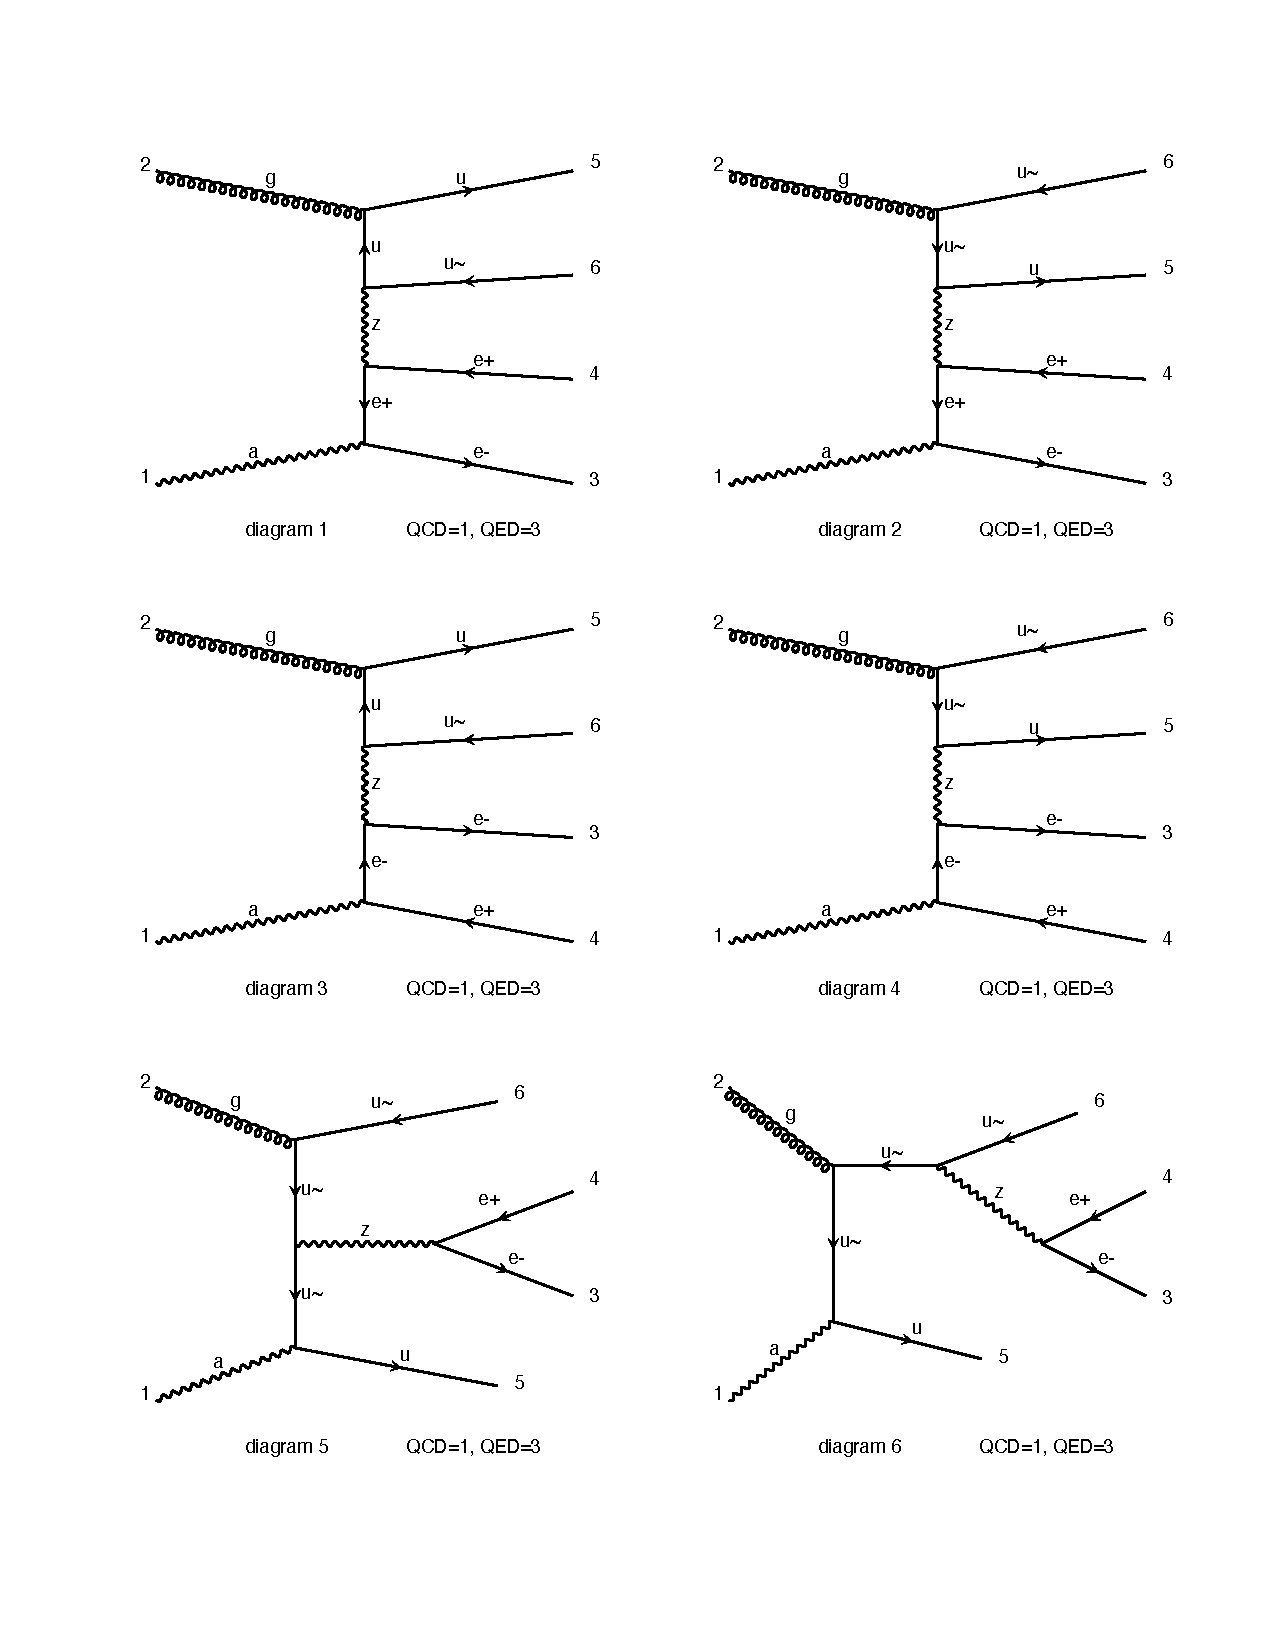
\includegraphics[width=0.7\textwidth]{diagrams_ag_channel_a}
      \caption{Examples of Feynman graphs contributing to the $\gamma g$ channel.}
  \label{fig:ag_a}
\end{figure}
%%%%%%%%%%%%%%%%%%%%%%
%%%%%%%%%%%figure%%%%%%%%%%
\begin{figure}[t]
    \centering
    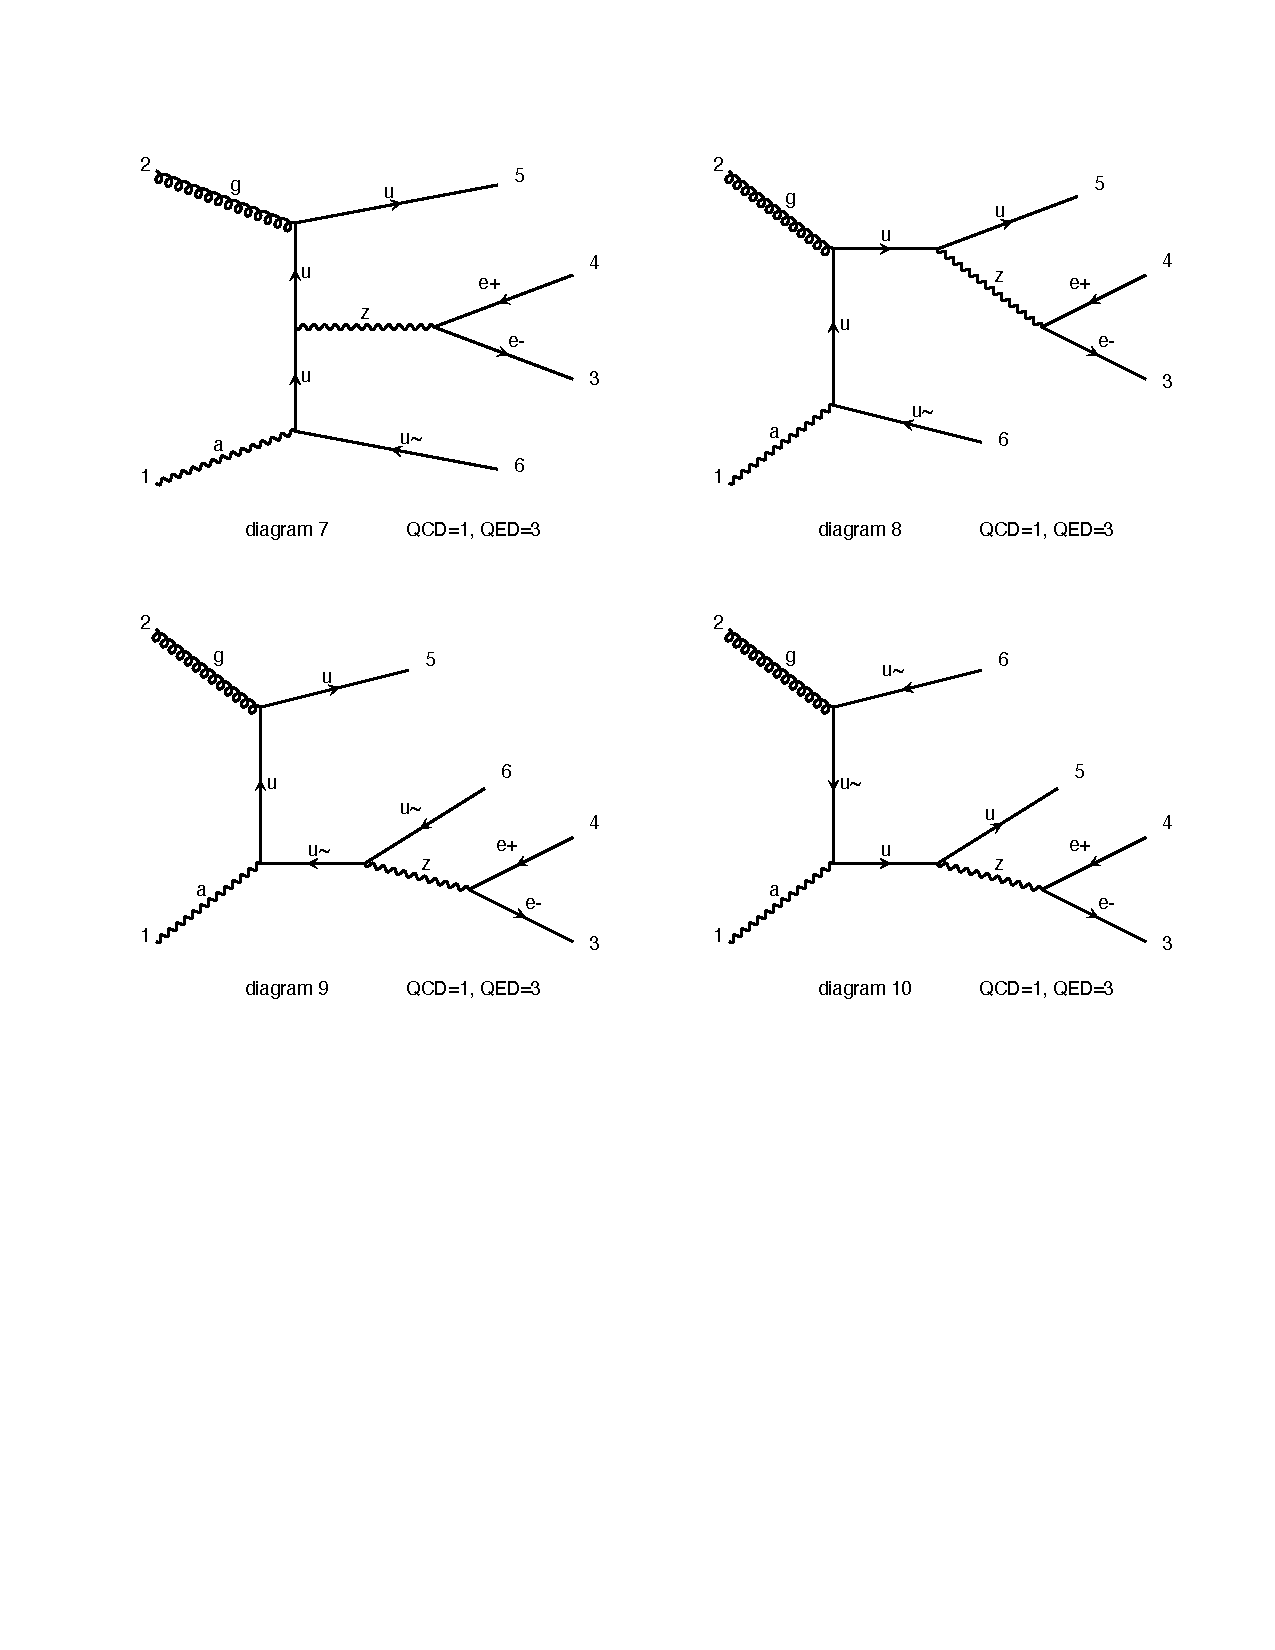
\includegraphics[width=0.7\textwidth]{diagrams_ag_channel_b}
    \caption{Examples of Feynman graphs contributing to the $\gamma g$ channel.}
  \label{fig:ag_b}
\end{figure}
%%%%%%%%%%%%%%%%%%%%%%




This partonic cross section can only receives contributions from real radiation and from pdf 
renormalisation, according to
\beq
d\hat{\sigma}_{\rm nnlo}^{\gamma g \rightarrow e^-e^+q\barq}
=
d\hat{\sigma}^{\gamma g \rightarrow e^-e^+q\barq}_{\rm rr}
+d\hat{\sigma}^{\gamma g \rightarrow e^-e^+q\barq}_{\rm pdf} \; ,
\eeq
where the double real term is 
\beq
2s\cdot d\hat{\sigma}_{rr}^{\gamma g \rightarrow e^-e^+q\barq} 
\equiv 
\int[dp_5] [dp_6] \, F_{LM}(1_\gamma,2_g,3_{e^-},4_{e^+} | 5_q, 6_{\bar{q}})  
\equiv 
\big\langle F_{LM}(1_\gamma,2_g,3_{e^-},4_{e^+} | 5_q, 6_{\bar{q}})\big\rangle \, .
\nn
\eeq
Let us stress that such term (as well as the complete partonic cross section)
is not affected by soft singularities, and therefore only collinear subtraction
is actually needed. We begin by listing all the collinear singularities that may 
arise:
\beq
C_{15}\, , \quad
C_{16} \, ,  \quad 
C_{25}\, ,  \quad
C_{26} \, ,  \quad
C_{26} \, C_{15}\, ,  \quad 
C_{16} \, C_{25}\, ,  \quad 
C_{25} \, C_{56,2}\, ,  \quad
C_{26} \, C_{56,2}\, .
\eeq
It is then evident that we need two double collinear sectors (dividing $C_{26} \, C_{15}$
from $C_{16} \, C_{25}$) and one triple collinear sector, that we will need to split
into two subpartitions (one containing the strongly ordered configurations
$C_{25} \, C_{56,2}$ and $C_{26} \, C_{56,2}$, respectively).
For the sake of transparency, we decide to introduce the same partition 
functions as in the previous channel (thus including two triple collinear
sectors)
\beq
1 = \omega^{51,61}+ \omega^{52,62} + \omega^{52,61} + \omega^{51,62} \, ,
\label{eq:partition_ag_temp} 
\eeq
where the explicit expressions for the objects appearing above are 
given in Eq.\eqref{eq:partition_explicit_aq}. We stress that, in the present
case, such a choice is "non-minimal" and could be further optimised. 
However, in order to speed up the computations that follows, we decided
to adopt the same partition we have already exploited before.
As mentioned, the sector $5262$ is characterised by two overlapping 
single collinear regimes, i.e. $C_{52}$ and $C_{62}$ and requires 
a further partitioning. We introduce two complementary theta functions
and write
\beq
1 = \omega^{51,61}+ \omega^{52,62} \big( \theta_A+\theta_C\big) + \omega^{52,61} + \omega^{51,62} \, ,
\label{eq:partition_ag} 
\eeq
with the following understanding
\beq
\begin{cases}
{\rm sector \; A} : \quad \theta^{62} < \theta^{52} \, ,
\\
{\rm sector \; C} : \quad \theta^{52} < \theta^{62} \, .
\end{cases}
\eeq
{\color{blue}{It is useful to split the triple collinear sector into
four subsectors. The reason is that we want to recycle the result
for the triple collinear integrated counterterm (strongly-ordered 
subtracted) from Max's paper. The computation there has
been performed for 4 subsectors ($a, b, c, d$). Readapting the 
final result to include only two subsector ($a, c$) would mean
to re-evaluate the strongly ordered contributions with a new
definition of $\theta_A$ and $\theta_C$. In the next pages we will
present the formulas for both cases, with the understanding that
the explicit expression for $P_{g \gamma}^{TC}$ for the two 
subsector case has not been jet computed. We will mark in blue
the terms that arise only in the four-subsector configuration. In 
particular we will use
\beq
1 = \omega^{51,61}+ \omega^{52,62} \big( \theta_A+\theta_B+\theta_C+\theta_D\big) + \omega^{52,61} + \omega^{51,62} \, ,
\label{eq:partition_ag} 
\eeq
with the following understanding
\beq
\begin{cases}
{\rm sector \; A} : \theta \big(\rho_{26} < \frac{\rho_{25}}{2} \big) \, ,
\\[3pt]
{\rm sector \; B} : \theta \big(\frac{\rho_{25}}{2}<\rho_{26} < \rho_{25} \big) \, ,
\\[3pt]
{\rm sector \; C} : \theta \big(\rho_{25} < \frac{\rho_{26}}{2} \big) \, , 
\\[3pt]
{\rm sector \; D} : \theta \big(\frac{\rho_{26}}{2}<\rho_{25} < \rho_{26} \big) \, .
\end{cases}
\eeq
}} \\
The limits enhanced in each sector are then 
\beq
\omega^{51,61}  &:&  C_{51}, \, C_{61}, \, \Chiara[\cancelto{0}{C_{56, 1}}]
\nn \\[0.2cm]
&& 
\quad 
\rightarrow \; \omega^{51,61}  
=  \big[  C_{51}+ C_{61} + C_{56, 1} (1-C_{51}-C_{61}) + (1-C_{56, 1}) (1-C_{51}-C_{61})  \big] \, \omega^{51,61}  \; ,
\nn \\[0.3cm]
%%
&&
\hspace{21mm}
=  \big[  C_{51}+ C_{61} + (1-C_{51}-C_{61})  \big] \, \omega^{51,61} 
\nn \\[0.3cm]
%%
\omega^{52,62} \, \theta_A  &:&  C_{62}, \, C_{56,2}
\nn \\[0.2cm]
&& 
\quad 
\rightarrow \; \omega^{52,62}  \, \theta_A  
=  \big[ C_{62} + C_{56, 2} (1-C_{62}) + (1-C_{56,2})  (1-C_{62})  \big] \, \omega^{52,62}  \, \theta_A 
\nn \\[0.2cm]
%%
{\color{blue}{\omega^{52,62} \, \theta_B}}  &:& \Chiara[\cancelto{0}{C_{56}}] \; \; \;  {\color{blue} , \, {C_{56,2}}}
\nn \\[0.2cm]
&& 
\quad
{\color{blue}{\rightarrow \; \omega^{52,62}  \, \theta_B  
=  \big[ C_{56, 2} + (1-C_{56,2})  \big] \, \omega^{52,62}  \, \theta_B }}
\nn \\[0.2cm]
%%
\omega^{52,62} \, \theta_C  &:& C_{52}, \, C_{56,2}
\nn \\[0.2cm]
&& 
\quad
\rightarrow \; \omega^{51,61} \, \theta_C 
=\big[ C_{52} + C_{56,2} (1-C_{52}) + (1-C_{56,2})  (1-C_{52})  \big] \,  \omega^{52,62} \, \theta_C
\nn \\[0.2cm]
%%
{\color{blue}{\omega^{52,62} \, \theta_D}}  &:& \Chiara[\cancelto{0}{C_{56}}] \; \; \;  {\color{blue} , \, {C_{56,2}}}
\nn \\[0.2cm]
&& 
\quad
{\color{blue}{\rightarrow \; \omega^{52,62}  \, \theta_D 
=  \big[ C_{56, 2} + (1-C_{56,2})  \big] \, \omega^{52,62}  \, \theta_D }}
\nn \\[0.2cm]
%%
\omega^{51,62} &:& C_{51}, \, C_{62}
\nn \\[0.2cm]
&& 
\quad
\rightarrow \; \omega^{51,62}
= \big[ C_{51} + C_{62} -  C_{62} \, C_{51} + (1-C_{62})  (1-C_{51})  \big] \, 
 \omega^{51,62} 
\nn \\[0.2cm] 
%%
\omega^{52,61} &:& C_{52}, \, C_{61}
\nn \\[0.2cm]
&& 
\quad 
\rightarrow \; \omega^{52,61} =
\big[ C_{52} + C_{61} -  C_{52} \, C_{61} 
+ (1-C_{52})  (1-C_{61}) \big] \, \omega^{52,61}  \; .
\eeq
At this point we reorganise, as usual, the limits according to the
corresponding kinematics. We obtain
\beq
1 = \Omega^{\, \gamma g} =
\Omega^{\, \gamma g}_1
+ \Omega^{\, \gamma g}_2
+ \Omega^{\, \gamma g}_3
+ \Omega^{\, \gamma g}_4    \; , 
\eeq 
where the projection operators are defined as
\beq
\Omega^{\, \gamma g}_1 
&=&
(1-C_{51}-C_{61}) \, \omega^{51,61}  
  \nn \\
  &&
  + \, 
  (1-C_{56,2})\,  (1-C_{62})\, \omega^{52,62}  \, \theta_A 
  +
   (1-C_{56,2})  (1-C_{52}) \,  \omega^{52,62} \, \theta_C 
  \nn \\
  && 
  + (1-C_{62}) \,(1-C_{51}) \, \omega^{51,62} 
   + (1-C_{61}) \,(1-C_{52}) \, \omega^{52,61}
   \nn \\
   &&
   {\color{blue}{
   +  \, 
   (1-C_{56,2})\, \omega^{52,62}  \, \theta_B 
  +
   (1-C_{56,2})\, \omega^{52,62} \, \theta_D }}
     \; , 
    \nn \\[10pt]
  %%%%%%%%%%%%%%%%%%%%%%%%%%%%
  \Omega^{\, \gamma g}_2
&=&
 C_{56,2} \, (1-C_{62}) \,  \omega^{52,62} \, \theta_A 
 +
 C_{56,2} (1-C_{52}) \,  \omega^{52,62} \, \theta_C
 \nn \\
 &&
 \color{blue}{
 + \, 
 C_{56,2} \,  \omega^{52,62} \, \theta_B
 +
 C_{56,2} \, \omega^{52,62} \, \theta_D } \; ,
   \nn \\[10pt]
  %%%%%%%%%%%%%%%%%%%%%%%%%%%%
  \Omega^{\, \gamma g}_3
&=&
-  \, C_{52} \, C_{61}  \, \omega^{52,61}
-  C_{51} \, C_{62}  \, \omega^{51,62} \; ,
   \nn \\[10pt]
  %%%%%%%%%%%%%%%%%%%%%%%%%%%%
    \Omega^{\, \gamma g}_4
&=&
 C_{62}  \, 
 (  \omega^{51,62} 
  +  \omega^{52,62} \, \theta_A)
 +
 C_{52}  \, \big(  \omega^{52,61} + 
 \omega^{52,62} \, \theta_C  \big)
 \nn \\
  &&
 + \, 
  C_{61} \, \big(  \omega^{52,61} +
 \omega^{51,61}  \big)
 +  C_{51} \, \big(  \omega^{51,61} +
 \omega^{51,62}  \big) \; .
\eeq
Given this choice of phase space partitioning, we can rewrite the soft-regulated contributions as
\beq
\big\langle F_{LM}(1_\gamma,2_g,3_{e^-},4_{e^+} | 5_q, 6_{\bar{q}})\big\rangle
&=& 
\big\langle  \Omega^{\, \gamma g} \, F_{LM}(1_\gamma,2_g,3_{e^-},4_{e^+} | 5_q, 6_{\bar{q}})\big\rangle
\nn \\
&=&
\sum_{i=1}^4
\big\langle   \Omega^{\, \gamma g}_i \, F_{LM}(1_\gamma,2_g,3_{e^-},4_{e^+} | 5_q, 6_{\bar{q}})\big\rangle
\; .
\nn 
\eeq

\subsection{Real contribution}
Here we report the formulas relevant for the subtraction of the $\gamma g$
channel.

\subsubsection{Triple collinear}
We begin with the triple collinear limit, which can be borrowed from the results deduced in the NNLO QCD case. We have
\beq
 \big\langle 
 \Omega^{\gamma g}_2
\, F_{LM}(1_\gamma,2_g,3_{e^-},4_{e^+} | 5_q, 6_{\bar{q}})
\big\rangle 
&=&
\frac{ [\alpha_s] [\alpha]  T_R \, Q_q^2}{\eps} \, 
 (2 E_2)^{-4\eps} \; \times
 \nn \\
 && \hspace{-3cm }\times \; 
\int_0^1 dz \, P_{g \gamma}^{TC}\big(z,E_2\big)
\Big\langle
\frac{F_{LM}(1_\gamma,z\cdot2_\gamma,3_{e^-},4_{e^+})}{z}
\Big\rangle
\, ,
\eeq
where $ P_{g \gamma}^{TC}$ have to be deduced from Max's paper.
(\Chiara[CAVEAT: the result can be taken without modification
from Max's paper only if we adopt a four-subsectors partition
of the triple collinear sector. Otherwise we need to re-evaluate the
strongly-ordered limits.]).

 \subsubsection{Double collinear}
 The contribution to integrate reads
 \beq
 \big\langle 
 \Omega^{\gamma g}_3
\, F_{LM}(1_\gamma,2_g,3_{e^-},4_{e^+} | 5_q, 6_{\bar{q}})
\big\rangle 
&=&
-  
\big\langle
C_{52} \, C_{61}  \, \omega^{52,61}
 \, F_{LM}(1_\gamma,2_g,3_{e^-},4_{e^+} | 5_q, 6_{\bar{q}})
\big\rangle 
\nn \\
&&
- \,  \big\langle
C_{51} \, C_{62}  \, \omega^{51,62} 
 \, F_{LM}(1_\gamma,2_g,3_{e^-},4_{e^+} | 5_q, 6_{\bar{q}})
\big\rangle \; .
\qquad
 \eeq
Thanks to the symmetry of the problem, the two terms
return identical contributions, up to an exchange
$q \leftrightarrow \barq$ in the Born matrix element
 \beq
 &&
 \hspace{-15mm}
 -  
\big\langle
C_{52} \, C_{61}  \, \omega^{52,61}
 \, F_{LM}(1_\gamma,2_g,3_{e^-},4_{e^+} | 5_q, 6_{\bar{q}})
\big\rangle 
=
\nn \\
&& =
\Big\langle
C_{52}
\bigg[
\frac{[\alpha_{b}]}{\eps}\, Q_q^2 \, N_c \, (2E_1)^{-2\eps} \, 
\int_{0}^1 dz \, 
P_{\barq g}^{\rm NLO} (z) \, 
\frac{F_{LM}(z\cdot 1_{q},2_g,3_{e^-},4_{e^+}|5_q)}{z} 
\bigg]
\Big\rangle
\nn \\
&& =
-
\frac{[\alpha_{s, b}] [\alpha_{b}]}{\eps^2}\, Q_q^2 \, N_c \, T_R \, 
(2E_1)^{-2\eps} \, 
(2E_2)^{-2\eps} \,  \times
\nn \\
&& \qquad \times \; 
\int_{0}^1 dz_1 \, dz_2 \, 
P_{\barq g}^{\rm NLO} (z_1) \, 
P_{\barq g}^{\rm NLO} (z_2) \, 
\Big\langle
\frac{F_{LM}(z_1\cdot 1_{q},z_2 \cdot 2_\barq,3_{e^-},4_{e^+})}{z_1 \, z_2} 
\Big\rangle \; ,
\nn \\
&&
 \hspace{-15mm}
-  
\big\langle
C_{51} \, C_{62}  \, \omega^{51,62}
 \, F_{LM}(1_\gamma,2_g,3_{e^-},4_{e^+} | 5_q, 6_{\bar{q}})
\big\rangle 
=
\nn \\
&& =
-
\frac{[\alpha_{s, b}] [\alpha_{b}]}{\eps^2}\, Q_q^2 \, N_c \, T_R \, 
(2E_1)^{-2\eps} \, 
(2E_2)^{-2\eps} \,  \times
\nn \\
&& \qquad \times \; 
\int_{0}^1 dz_1 \, dz_2 \, 
P_{\barq g}^{\rm NLO} (z_1) \, 
P_{\barq g}^{\rm NLO} (z_2) \, 
\Big\langle
\frac{F_{LM}(z_1\cdot 1_\barq,z_2 \cdot 2_q,3_{e^-},4_{e^+})}{z_1 \, z_2} 
\Big\rangle \; .
 \eeq
 The full result reads
 \beq
 && \hspace{-7mm} 
 \big\langle 
 \Omega^{\gamma g}_3
\, F_{LM}(1_\gamma,2_g,3_{e^-},4_{e^+} | 5_q, 6_{\bar{q}})
\big\rangle =
\nn \\
&& =
-
\frac{[\alpha_{s, b}] [\alpha_{b}]}{\eps^2}\, Q_q^2 \, N_c \, T_R \, 
(2E_1)^{-2\eps} \, 
(2E_2)^{-2\eps} \, 
\int_{0}^1 dz_1 \, dz_2 \, 
P_{\barq g}^{\rm NLO} (z_1) \, 
P_{\barq g}^{\rm NLO} (z_2) \, 
 \times
\nn \\
&& \qquad \times \; 
\bigg[
\Big\langle
\frac{F_{LM}(z_1\cdot 1_q,z_2 \cdot 2_\barq,3_{e^-},4_{e^+})}{z_1 \, z_2} 
\Big\rangle
+
\Big\langle
\frac{F_{LM}(z_1\cdot 1_\barq,z_2 \cdot 2_q,3_{e^-},4_{e^+})}{z_1 \, z_2} 
\Big\rangle
\bigg]
 \eeq

  \subsubsection{Single collinear}
 here we turn to the single soft component, which is given by
 \beq
 \big\langle 
 \Omega^{\gamma g}_4
\, F_{LM}(1_\gamma,2_g,3_{e^-},4_{e^+} | 5_q, 6_{\bar{q}})
\big\rangle 
\eeq
with
\beq
 \Omega^{\gamma g}_4
 &=&
 {\color{orange}{
 C_{62}  \, 
 (  \omega^{51,62} 
  +  \omega^{52,62} \, \theta_A)
  }}
 +
 {\color{brown}{
 C_{52}  \, \big(  \omega^{52,61} + 
 \omega^{52,62} \, \theta_C  \big)
 }}
 \nn \\
  &&
 + \, 
{\color{cyan}{
 C_{61} \, \big(  \omega^{52,61} +
 \omega^{51,61}  \big)
 }}
 +  
 {\color{purple}{
 C_{51} \, \big(  \omega^{51,61} +
 \omega^{51,62}  \big) 
 }}
 \; .
\eeq
We analyse the terms above in order.
Beginning with
 \beq
 \big\langle 
{\color{orange}{
 C_{62}  \, 
 (  \omega^{51,62} 
  +  \omega^{52,62} \, \theta_A)
  }}
\, F_{LM}(1_\gamma,2_g,3_{e^-},4_{e^+} | 5_q, 6_{\bar{q}})
\big\rangle  \, ,
\eeq
 we have
  \beq
  && \hspace{-7mm}
 \big\langle 
{\color{orange}{
 C_{62}  \, 
  \omega^{51,62} 
  }}
\, F_{LM}(1_\gamma,2_g,3_{e^-},4_{e^+} | 5_q, 6_{\bar{q}})
\big\rangle  
=
\nn \\
&& =
-
\frac{[\alpha_{s,b}]}{\eps}\, T_R \, (2E_1)^{-2\eps} \, 
\int_{0}^1 dz \, 
P_{\barq g}^{\rm NLO} (z) \, 
\Big\langle
\tilde {\omega}^{51,62}_{6\parallel 2} \;
\frac{F_{LM}( 1_{\gamma}, z\cdot2_q,3_{e^-},4_{e^+}|5_q)}{z} 
\Big\rangle
\nn \\
&& =
-
\frac{[\alpha_{s,b}]}{\eps}\, T_R \, (2E_1)^{-2\eps} \, 
\int_{0}^1 dz \, 
P_{\barq g}^{\rm NLO} (z) \,
\Big[
\mathcal{O}_{\rm nlo}^q
+ C_{51}
\Big] 
\Big\langle
\tilde {\omega}^{51,62}_{6\parallel 2} \;
\frac{F_{LM}( 1_{\gamma}, z\cdot2_q,3_{e^-},4_{e^+}|5_q)}{z} 
\Big\rangle
\nn \\
&& =
-
\frac{[\alpha_{s,b}]}{\eps}\, T_R \, (2E_1)^{-2\eps} \, 
\int_{0}^1 dz \, 
P_{\barq g}^{\rm NLO} (z) \,
\mathcal{O}_{\rm nlo}^q \; 
\Big\langle
\tilde {\omega}^{51,62}_{6\parallel 2} \;
\frac{F_{LM}( 1_{\gamma}, z\cdot2_q,3_{e^-},4_{e^+}|5_q)}{z} 
\Big\rangle
\nn \\
&& \quad
+ \, 
\frac{[\alpha_{s,b}] [\alpha_{b}]}{\eps^2} \, Q_q^2\,N_c \,  T_R \;
\frac{\Gamma^2(1-\eps)}{\Gamma(1-2\eps)} \; 
(2E_1)^{-2\eps} \, 
(2E_2)^{-2\eps} \; \times
\nn \\
&& \qquad \quad \times
\int_{0}^1 dz_1 \, dz_2 \, 
P_{\barq g}^{\rm NLO} (z_1) \,
P_{\barq g}^{\rm NLO} (z_2) \,
\Big\langle
\frac{F_{LM}(z_1\cdot 1_\barq, z_2\cdot2_q,3_{e^-},4_{e^+}|5_q)}{z_1 \, z_2} 
\Big\rangle
\nn
\, .
\eeq
For the remaining term we follows the computation in Eq.\eqref{eq:Cg1_wa1g1_thetaA}
and get
  \beq
    && \hspace{-7mm}
 \big\langle 
{\color{orange}{
 C_{62}  \,  \omega^{52,62} \, \theta_A
  }}
\, F_{LM}(1_\gamma,2_g,3_{e^-},4_{e^+} | 5_q, 6_{\bar{q}})
\big\rangle
=
\nn \\
&&
= 
-
\frac{[\alpha_{s,b}]}{\eps}\, T_R \, (2E_2)^{-2\eps} \, 
\int_{0}^1 dz \, 
P_{\barq g}^{\rm NLO} (z) \, 
\Big\langle
\tilde {\omega}^{52,62}_{6\parallel 2} \;
\Big(\frac{\rho_{52}}{2}
\Big)^{-\eps} \; 
\frac{F_{LM}( 1_{\gamma}, z\cdot2_q,3_{e^-},4_{e^+}|5_q)}{z} 
\Big\rangle
\nn \\
&&
= 
-
\frac{[\alpha_{s,b}]}{\eps}\, T_R \, (2E_2)^{-2\eps} \, 
\int_{0}^1 dz \, 
P_{\barq g}^{\rm NLO} (z) \, 
\mathcal{O}_{\rm nlo}^{q}\; 
\Big\langle
\tilde {\omega}^{52,62}_{6\parallel 2} \;
\Big(\frac{\rho_{52}}{2}
\Big)^{-\eps} \; 
\frac{F_{LM}( 1_{\gamma}, z\cdot2_q,3_{e^-},4_{e^+}|5_q)}{z} 
\Big\rangle 
\nn  \\
&&
\qquad
-
\frac{[\alpha_{s,b}]}{\eps}\, T_R \, (2E_2)^{-2\eps} \, 
\int_{0}^1 dz \, 
P_{\barq g}^{\rm NLO} (z) \, 
C_{52} \; 
\Big\langle
\Big(\frac{\rho_{52}}{2}
\Big)^{-\eps} \; 
\frac{F_{LM}( 1_{\gamma}, z\cdot2_q,3_{e^-},4_{e^+}|5_q)}{z} 
\Big\rangle \nn \\
&&
=
-
\frac{[\alpha_{s,b}]}{\eps}\, T_R \, (2E_2)^{-2\eps} \, 
\int_{0}^1 dz \, 
P_{\barq g}^{\rm NLO} (z) \, 
\mathcal{O}_{\rm nlo}^{q}\; 
\Big\langle
\tilde {\omega}^{52,62}_{6\parallel 2} \;
\Big(\frac{\rho_{52}}{2}
\Big)^{-\eps} \; 
\frac{F_{LM}( 1_{\gamma}, z\cdot2_q,3_{e^-},4_{e^+}|5_q)}{z} 
\Big\rangle 
\nn  \\
&&
\qquad
+
\frac{[\alpha_b] [\alpha_{s,b}] \, T_R \, Q_q^2}{2\eps^2} \,  
 \frac{ \Gamma(1-\eps) \, \Gamma(1-2\eps)}{\Gamma(1-3\eps)} \, 
 (2E_2)^{-4\eps} \, \times
 \nn \\
 && \qquad \qquad \times
\int_{0}^1 dz \, 
\big[
P_{\barq g}^{\rm NLO}
\otimes
P_{q\gamma}^{\rm NLO}
\big] (z, E_2) \, 
\Big\langle
\frac{F_{LM}(1_\gamma, z\cdot 2_\gamma,3_{e^-},4_{e^+} )}{z} \Big\rangle \; .
\eeq
The full $C_{62}$ contribution reads
 \beq
 &&
 \hspace{-7mm}
 \big\langle 
{\color{orange}{
 C_{62}  \, 
 (  \omega^{51,62} 
  +  \omega^{52,62} \, \theta_A)
  }}
\, F_{LM}(1_\gamma,2_g,3_{e^-},4_{e^+} | 5_q, 6_{\bar{q}})
\big\rangle 
=
\nn \\
&& =
-
\frac{[\alpha_{s,b}]}{\eps}\, T_R \, (2E_2)^{-2\eps} \, 
\int_{0}^1 dz \, 
P_{\barq g}^{\rm NLO} (z) \,
\mathcal{O}_{\rm nlo}^q \; 
\Big\langle
\tilde {\omega}^{51,62}_{6\parallel 2} \;
\frac{F_{LM}( 1_{\gamma}, z\cdot2_q,3_{e^-},4_{e^+}|5_q)}{z} 
\Big\rangle
\nn \\
&& \quad
+ \, 
\frac{[\alpha_{s,b}] [\alpha_{b}]}{\eps^2}\, Q_q^2 \,N_c \,  T_R \;
\frac{\Gamma^2(1-\eps)}{\Gamma(1-2\eps)} \; 
(2E_1)^{-2\eps} \, 
(2E_2)^{-2\eps} \; \times
\nn \\
&& \qquad \quad \times
\int_{0}^1 dz_1 \, dz_2 \, 
P_{\barq g}^{\rm NLO} (z_1) \,
P_{\barq g}^{\rm NLO} (z_2) \,
\Big\langle
\frac{F_{LM}(z_1\cdot 1_\barq, z_2\cdot2_q,3_{e^-},4_{e^+})}{z_1 \, z_2} 
\Big\rangle
\nn \\
&&
\quad
-
\frac{[\alpha_{s,b}]}{\eps}\, T_R \, (2E_2)^{-2\eps} \, 
\int_{0}^1 dz \, 
P_{\barq g}^{\rm NLO} (z) \, 
\mathcal{O}_{\rm nlo}^{q}\; 
\Big\langle
\tilde {\omega}^{52,62}_{6\parallel 2} \;
\Big(\frac{\rho_{52}}{2}
\Big)^{-\eps} \; 
\frac{F_{LM}( 1_{\gamma}, z\cdot2_q,3_{e^-},4_{e^+}|5_q)}{z} 
\Big\rangle 
\nn  \\
&&
\quad
+
\frac{[\alpha_b] [\alpha_{s,b}] \, T_R \, Q_q^2}{2\eps^2} \,  
 \frac{ \Gamma(1-\eps) \, \Gamma(1-2\eps)}{\Gamma(1-3\eps)} \, 
 (2E_2)^{-4\eps} \, \times
 \nn \\
 && \qquad \qquad \times
\int_{0}^1 dz \, 
\big[
P_{\barq g}^{\rm NLO}
\otimes
P_{q\gamma}^{\rm NLO}
\big] (z) \, 
\Big\langle
\frac{F_{LM}(1_\gamma, z\cdot 2_\gamma,3_{e^-},4_{e^+} )}{z} \Big\rangle 
 \, .
\eeq
{\color{blue}{In the case of four subpartitions, the result for $C_{62}  \,  \omega^{52,62} \, \theta_A$ is slightly different, due to the 
different left-over factor from the $\theta$-function. The result for ($a, b, c, d$) is quoted below}} 
 \beq
 &&
 \hspace{-7mm}
 \big\langle 
{\color{orange}{
 C_{62}  \, 
 (  \omega^{51,62} 
  +  \omega^{52,62} \, \theta_A)
  }}
\, F_{LM}(1_\gamma,2_g,3_{e^-},4_{e^+} | 5_q, 6_{\bar{q}})
\big\rangle 
=
\nn \\
&& =
-
\frac{[\alpha_{s,b}]}{\eps}\, T_R \, (2E_2)^{-2\eps} \, 
\int_{0}^1 dz \, 
P_{\barq g}^{\rm NLO} (z) \,
\mathcal{O}_{\rm nlo}^q \; 
\Big\langle
\tilde {\omega}^{51,62}_{6\parallel 2} \;
\frac{F_{LM}( 1_{\gamma}, z\cdot2_q,3_{e^-},4_{e^+}|5_q)}{z} 
\Big\rangle
\nn \\
&& \quad
+ \, 
\frac{[\alpha_{s,b}] [\alpha_{b}]}{\eps^2}\, Q_q^2 \,N_c \,  T_R \;
\frac{\Gamma^2(1-\eps)}{\Gamma(1-2\eps)} \; 
(2E_1)^{-2\eps} \, 
(2E_2)^{-2\eps} \; \times
\nn \\
&& \qquad \quad \times
\int_{0}^1 dz_1 \, dz_2 \, 
P_{\barq g}^{\rm NLO} (z_1) \,
P_{\barq g}^{\rm NLO} (z_2) \,
\Big\langle
\frac{F_{LM}(z_1\cdot 1_\barq, z_2\cdot2_q,3_{e^-},4_{e^+})}{z_1 \, z_2} 
\Big\rangle
\nn \\
&&
\quad
-
\frac{[\alpha_{s,b}]}{\eps}\, T_R \, (2E_2)^{-2\eps} \, 
\int_{0}^1 dz \, 
P_{\barq g}^{\rm NLO} (z) \, 
\mathcal{O}_{\rm nlo}^{q}\; 
\Big\langle
\tilde {\omega}^{52,62}_{6\parallel 2} \;
\Big(\frac{
{\color{blue}{\eta_{52}}}}{2}
\Big)^{-\eps} \; 
\frac{F_{LM}( 1_{\gamma}, z\cdot2_q,3_{e^-},4_{e^+}|5_q)}{z} 
\Big\rangle 
\nn  \\
&&
\quad
+
\frac{[\alpha_b] [\alpha_{s,b}] \, T_R \, Q_q^2}{2\eps^2} \,  
 \frac{ {\color{blue}{2^\eps}} \, \Gamma(1-\eps) \, \Gamma(1-2\eps)}{\Gamma(1-3\eps)} \, 
 (2E_2)^{-4\eps} \, \times
 \nn \\
 && \qquad \qquad \times
\int_{0}^1 dz \, 
\big[
P_{\barq g}^{\rm NLO}
\otimes
P_{q\gamma}^{\rm NLO}
\big] (z) \, 
\Big\langle
\frac{F_{LM}(1_\gamma, z\cdot 2_\gamma,3_{e^-},4_{e^+} )}{z} \Big\rangle 
 \, .
\eeq
{\color{blue}{end of the contribution in the four-subpartition fashion.}} \\
We then move to the next object
  \beq
     && \hspace{-7mm}
 \big\langle 
{\color{brown}{
 C_{52}  \, \big(  \omega^{52,61} + 
 \omega^{52,62} \, \theta_C  \big)
 }}
\, F_{LM}(1_\gamma,2_g,3_{e^-},4_{e^+} | 5_q, 6_{\bar{q}})
\big\rangle  =
\nn \\
&&
=
-\frac{[\alpha_{s, b}]}{\eps} \; T_R \, (2E_2)^{-2\eps} \, 
\int_{0}^1 dz \, 
P^{\rm NLO}_{\bar{q}g} (z) \, 
\mathcal{O}_{\rm nlo}^{\barq}\,
\Big\langle 
\tilde{\omega}^{52,61}_{5\parallel 2} \; \frac{F_{LM}(1_\gamma,z\cdot2_\barq,3_{e^-},4_{e^+} | 6_{\bar{q}})}{z} \Big\rangle
\nn \\
&&
\quad
+ \, 
\frac{[\alpha_{s,b}] [\alpha_{b}]}{\eps^2} \, Q_q^2\,N_c \,  T_R \;
\frac{\Gamma^2(1-\eps)}{\Gamma(1-2\eps)} \; 
(2E_1)^{-2\eps} \, 
(2E_2)^{-2\eps} \; \times
\nn \\
&& \qquad \quad \times
\int_{0}^1 dz_1 \, dz_2 \, 
P_{\barq g}^{\rm NLO} (z_2) \,
P_{q\gamma}^{\rm NLO} (z_1) \,
\Big\langle
\frac{F_{LM}(z_1\cdot 1_q, z_2\cdot2_\barq,3_{e^-},4_{e^+})}{z_1 \, z_2} 
\Big\rangle 
\nn \\
&&
\quad
-
\frac{[\alpha_{s,b}]}{\eps}\, T_R \, (2E_2)^{-2\eps} \, 
\int_{0}^1 dz \, 
P_{\barq g}^{\rm NLO} (z) \, 
\mathcal{O}_{\rm nlo}^{\barq}
\Big\langle
\tilde {\omega}^{52,62}_{5\parallel 2} \;
\Big(\frac{\rho_{62}}{2}
\Big)^{-\eps} \; 
\frac{F_{LM}( 1_{\gamma}, z\cdot2_\barq,3_{e^-},4_{e^+}|6_\barq)}{z} 
\Big\rangle
\nn  \\
&&
\quad
+
\frac{[\alpha_b] [\alpha_{s,b}] \, T_R \, Q_q^2}{2\eps^2} \,  
 \frac{ \Gamma(1-\eps) \, \Gamma(1-2\eps)}{\Gamma(1-3\eps)} \, 
 (2E_2)^{-4\eps} \, \times
 \nn \\
 && \qquad \qquad \times
\int_{0}^1 dz \, 
\big[
P_{\barq g}^{\rm NLO}
\otimes
P_{q\gamma}^{\rm NLO}
\big] (z) \, 
\Big\langle
\frac{F_{LM}(1_\gamma, z\cdot 2_\gamma,3_{e^-},4_{e^+} )}{z} \Big\rangle
\, .
\eeq
where
   \beq
   && \hspace{-7mm}
 \big\langle 
{\color{brown}{
 C_{52}  \,  \omega^{52,61} 
 }}
\, F_{LM}(1_\gamma,2_g,3_{e^-},4_{e^+} | 5_q, 6_{\bar{q}})
\big\rangle =
\nn \\
%&& 
%=  
%-\frac{[\alpha_{s, b}]}{\eps} \; T_R \, (2E_2)^{-2\eps} \, 
%\int_{0}^1 dz \, 
%P^{\rm NLO}_{\bar{q}g} (z) \, 
%\mathcal{O}_{\rm nlo}^{\barq}\,
%\Big\langle 
%\tilde{\omega}^{52,61}_{5\parallel 2} \; \frac{F_{LM}(1_\gamma,z\cdot2_\barq,3_{e^-},4_{e^+} | 6_{\bar{q}})}{z} \Big\rangle
%\nn \\
%&&
%\quad
%-\frac{[\alpha_{s, b}]}{\eps} \; T_R \, (2E_2)^{-2\eps} \, 
%\int_{0}^1 dz_2 \, 
%P^{\rm NLO}_{\bar{q}g} (z_2) \, 
%C_{61}
%\Big\langle 
% \frac{F_{LM}(1_\gamma,z_2\cdot2_\barq,3_{e^-},4_{e^+} | 6_{\bar{q}})}{z_2} \Big\rangle
%\nn \\
&&
=  
-\frac{[\alpha_{s, b}]}{\eps} \; T_R \, (2E_2)^{-2\eps} \, 
\int_{0}^1 dz \, 
P^{\rm NLO}_{\bar{q}g} (z) \, 
\mathcal{O}_{\rm nlo}^{\barq}\,
\Big\langle 
\tilde{\omega}^{52,61}_{5\parallel 2} \; \frac{F_{LM}(1_\gamma,z\cdot2_\barq,3_{e^-},4_{e^+} | 6_{\bar{q}})}{z} \Big\rangle
\nn \\
&&
\quad
+ \, 
\frac{[\alpha_{s,b}] [\alpha_{b}]}{\eps^2} \, Q_q^2\,N_c \,  T_R \;
\frac{\Gamma^2(1-\eps)}{\Gamma(1-2\eps)} \; 
(2E_1)^{-2\eps} \, 
(2E_2)^{-2\eps} \; \times
\nn \\
&& \qquad \quad \times
\int_{0}^1 dz_1 \, dz_2 \, 
P_{\barq g}^{\rm NLO} (z_2) \,
P_{q\gamma}^{\rm NLO} (z_1) \,
\Big\langle
\frac{F_{LM}(z_1\cdot 1_q, z_2\cdot2_\barq,3_{e^-},4_{e^+})}{z_1 \, z_2} 
\Big\rangle \; ,
\eeq
and 
 \beq
 && \hspace{-0.7mm}
 \big\langle 
{\color{brown}{
 C_{52}  \, \omega^{52,62} \, \theta_C \, 
 }}
\, F_{LM}(1_\gamma,2_g,3_{e^-},4_{e^+} | 5_q, 6_{\bar{q}})
\big\rangle  
\nn \\
%&&
%=
%-
%\frac{[\alpha_{s,b}]}{\eps}\, T_R \, (2E_2)^{-2\eps} \, 
%\int_{0}^1 dz \, 
%P_{\barq g}^{\rm NLO} (z) \, 
%\Big\langle
%\tilde {\omega}^{52,62}_{5\parallel 2} \;
%\Big(\frac{\rho_{62}}{2}
%\Big)^{-\eps} \; 
%\frac{F_{LM}( 1_{\gamma}, z\cdot2_\barq,3_{e^-},4_{e^+}|6_\barq)}{z} 
%\Big\rangle
%\nn \\
%&&
%= 
%-
%\frac{[\alpha_{s,b}]}{\eps}\, T_R \, (2E_2)^{-2\eps} \, 
%\int_{0}^1 dz \, 
%P_{\barq g}^{\rm NLO} (z) \, 
%\mathcal{O}_{\rm nlo}^{\barq}
%\Big\langle
%\tilde {\omega}^{52,62}_{5\parallel 2} \;
%\Big(\frac{\rho_{62}}{2}
%\Big)^{-\eps} \; 
%\frac{F_{LM}( 1_{\gamma}, z\cdot2_\barq,3_{e^-},4_{e^+}|6_\barq)}{z} 
%\Big\rangle
%\nn  \\
%&&
%\qquad
%-
%\frac{[\alpha_{s,b}]}{\eps}\, T_R \, (2E_2)^{-2\eps} \, 
%\int_{0}^1 dz \, 
%P_{\barq g}^{\rm NLO} (z) \, 
%C_{62} \; 
%\Big\langle
%\Big(\frac{\rho_{62}}{2}
%\Big)^{-\eps} \; 
%\frac{F_{LM}( 1_{\gamma}, z\cdot2_\barq,3_{e^-},4_{e^+}|6_\barq)}{z} 
%\Big\rangle \nn \\[0.8cm]
&&
=
-
\frac{[\alpha_{s,b}]}{\eps}\, T_R \, (2E_2)^{-2\eps} \, 
\int_{0}^1 dz \, 
P_{\barq g}^{\rm NLO} (z) \, 
\mathcal{O}_{\rm nlo}^{\barq}
\Big\langle
\tilde {\omega}^{52,62}_{5\parallel 2} \;
\Big(\frac{\rho_{62}}{2}
\Big)^{-\eps} \; 
\frac{F_{LM}( 1_{\gamma}, z\cdot2_\barq,3_{e^-},4_{e^+}|6_\barq)}{z} 
\Big\rangle
\nn  \\
&&
\qquad
+
\frac{[\alpha_b] [\alpha_{s,b}] \, T_R \, Q_q^2}{2\eps^2} \,  
 \frac{ \Gamma(1-\eps) \, \Gamma(1-2\eps)}{\Gamma(1-3\eps)} \, 
 (2E_2)^{-4\eps} \, \times
 \nn \\
 && \qquad \qquad \times
\int_{0}^1 dz \, 
\big[
P_{\barq g}^{\rm NLO}
\otimes
P_{q\gamma}^{\rm NLO}
\big] (z, E_2) \, 
\Big\langle
\frac{F_{LM}(1_\gamma, z\cdot 2_\gamma,3_{e^-},4_{e^+} )}{z} \Big\rangle \; .
\eeq
{\color{blue}{In the case of four subpartitions, the result for $C_{62}  \,  \omega^{52,62} \, \theta_C$ is slightly different, due to the 
different left-over factor from the $\theta$-function. The result for ($a, b, c, d$) is quoted below}} 
  \beq
     && \hspace{-7mm}
 \big\langle 
{\color{brown}{
 C_{52}  \, \big(  \omega^{52,61} + 
 \omega^{52,62} \, \theta_C  \big)
 }}
\, F_{LM}(1_\gamma,2_g,3_{e^-},4_{e^+} | 5_q, 6_{\bar{q}})
\big\rangle  =
\nn \\
&&
=
-\frac{[\alpha_{s, b}]}{\eps} \; T_R \, (2E_2)^{-2\eps} \, 
\int_{0}^1 dz \, 
P^{\rm NLO}_{\bar{q}g} (z) \, 
\mathcal{O}_{\rm nlo}^{\barq}\,
\Big\langle 
\tilde{\omega}^{52,61}_{5\parallel 2} \; \frac{F_{LM}(1_\gamma,z\cdot2_\barq,3_{e^-},4_{e^+} | 6_{\bar{q}})}{z} \Big\rangle
\nn \\
&&
\quad
+ \, 
\frac{[\alpha_{s,b}] [\alpha_{b}]}{\eps^2} \, Q_q^2\,N_c \,  T_R \;
\frac{\Gamma^2(1-\eps)}{\Gamma(1-2\eps)} \; 
(2E_1)^{-2\eps} \, 
(2E_2)^{-2\eps} \; \times
\nn \\
&& \qquad \quad \times
\int_{0}^1 dz_1 \, dz_2 \, 
P_{\barq g}^{\rm NLO} (z_2) \,
P_{q\gamma}^{\rm NLO} (z_1) \,
\Big\langle
\frac{F_{LM}(z_1\cdot 1_q, z_2\cdot2_\barq,3_{e^-},4_{e^+})}{z_1 \, z_2} 
\Big\rangle 
\nn \\
&&
\quad
-
\frac{[\alpha_{s,b}]}{\eps}\, T_R \, (2E_2)^{-2\eps} \, 
\int_{0}^1 dz \, 
P_{\barq g}^{\rm NLO} (z) \, 
\mathcal{O}_{\rm nlo}^{\barq}
\Big\langle
\tilde {\omega}^{52,62}_{5\parallel 2} \;
\Big(\frac{{\color{blue}{\eta_{62}}}}{2}
\Big)^{-\eps} \; 
\frac{F_{LM}( 1_{\gamma}, z\cdot2_\barq,3_{e^-},4_{e^+}|6_\barq)}{z} 
\Big\rangle
\nn  \\
&&
\quad
+
\frac{[\alpha_b] [\alpha_{s,b}] \, T_R \, Q_q^2}{2\eps^2} \,  
 \frac{
 {\color{blue}{2^\eps}} \, 
 \Gamma(1-\eps) \, \Gamma(1-2\eps)}{\Gamma(1-3\eps)} \, 
 (2E_2)^{-4\eps} \, \times
 \nn \\
 && \qquad \qquad \times
\int_{0}^1 dz \, 
\big[
P_{\barq g}^{\rm NLO}
\otimes
P_{q\gamma}^{\rm NLO}
\big] (z) \, 
\Big\langle
\frac{F_{LM}(1_\gamma, z\cdot 2_\gamma,3_{e^-},4_{e^+} )}{z} \Big\rangle
\, .
\eeq
{\color{blue}{End of the four-subpartition result.}} \\
We can then move on and analyse
 \beq
     && \hspace{-7mm}
 \big\langle 
{\color{cyan}{
 C_{61} \, \big(  \omega^{52,61} +
 \omega^{51,61}  \big)
 }}
\, F_{LM}(1_\gamma,2_g,3_{e^-},4_{e^+} | 5_q, 6_{\bar{q}})
\big\rangle  =
\nn \\
&&
=
-\frac{[\alpha_{b}]}{\eps} \; Q_q^2 \,  N_c \, (2E_1)^{-2\eps} \, 
\int_{0}^1 dz \, 
P^{\rm NLO}_{\bar{q}g} (z) \, 
\mathcal{O}_{\rm nlo}^{\barq}\,
\Big\langle 
\tilde{\omega}^{52,61}_{6\parallel 1} \; \frac{F_{LM}(z\cdot 1_q,2_g,3_{e^-},4_{e^+} | 5_q)}{z} \Big\rangle
\nn \\
&&
\quad
+\frac{[\alpha_{b}][\alpha_{s,b}]}{\eps^2} \; Q_q^2 \,  N_c \,  T_R \, 
\frac{\Gamma^2(1-\eps)}{\Gamma(1-2\eps)} \; 
(2E_1)^{-2\eps} \,  (2E_2)^{-2\eps} \, \times
\nn \\
&& \qquad \times \; 
\int_{0}^1 dz_1 \, 
P^{\rm NLO}_{\bar{q}g} (z_1) \, 
P^{\rm NLO}_{\bar{q}g} (z_2) \, 
\Big\langle 
 \frac{F_{LM}(z_1\cdot 1_q,z_2 \cdot 2_\barq,3_{e^-},4_{e^+})}{z_1 \, z_2} \Big\rangle
 \nn \\
 &&
 \quad
 -\frac{[\alpha_{b}]}{\eps} \; Q_q^2 \,  N_c \, (2E_1)^{-2\eps} \, 
\int_{0}^1 dz \, 
P^{\rm NLO}_{\bar{q}g} (z) \, 
\Big\langle 
\tilde{\omega}^{51,61}_{6\parallel 1} \; \frac{F_{LM}(z\cdot 1_q,2_g,3_{e^-},4_{e^+} | 5_q)}{z} \Big\rangle 
\eeq
%%%%%%%%%
with
 \beq
     && \hspace{-7mm}
 \big\langle 
{\color{cyan}{
 C_{61} \, \omega^{52,61} 
  }}
\, F_{LM}(1_\gamma,2_g,3_{e^-},4_{e^+} | 5_q, 6_{\bar{q}})
\big\rangle  =
\nn \\
&&
= 
-\frac{[\alpha_{b}]}{\eps} \; Q_q^2 \,  N_c \, (2E_1)^{-2\eps} \, 
\int_{0}^1 dz \, 
P^{\rm NLO}_{\bar{q}g} (z) \, 
\mathcal{O}_{\rm nlo}^{\barq}\,
\Big\langle 
\tilde{\omega}^{52,61}_{6\parallel 1} \; \frac{F_{LM}(z\cdot 1_q,2_g,3_{e^-},4_{e^+} | 5_q)}{z} \Big\rangle
\nn \\
&&
\quad
+\frac{[\alpha_{b}][\alpha_{s,b}]}{\eps^2} \; Q_q^2 \,  N_c \,  T_R \, 
\frac{\Gamma^2(1-\eps)}{\Gamma(1-2\eps)} \; 
(2E_1)^{-2\eps} \,  (2E_2)^{-2\eps} \, \times
\nn \\
&& \qquad \times \; 
\int_{0}^1 dz_1 \, 
P^{\rm NLO}_{\bar{q}g} (z_1) \, 
P^{\rm NLO}_{\bar{q}g} (z_2) \, 
\Big\langle 
 \frac{F_{LM}(z_1\cdot 1_q,z_2 \cdot 2_\barq,3_{e^-},4_{e^+})}{z_1} \Big\rangle \; ,
\eeq
%%%%%%%%%%%
and
\beq
     && \hspace{-7mm}
 \big\langle 
{\color{cyan}{
 C_{61} \, \omega^{51,61} 
  }}
\, F_{LM}(1_\gamma,2_g,3_{e^-},4_{e^+} | 5_q, 6_{\bar{q}})
\big\rangle  =
\nn \\
&&
= 
-\frac{[\alpha_{b}]}{\eps} \; Q_q^2 \,  N_c \, (2E_1)^{-2\eps} \, 
\int_{0}^1 dz \, 
P^{\rm NLO}_{\bar{q}g} (z) \, 
\Big\langle 
\tilde{\omega}^{51,61}_{6\parallel 1} \; \frac{F_{LM}(z\cdot 1_q,2_g,3_{e^-},4_{e^+} | 5_q)}{z} \Big\rangle  \; .
\eeq
In full analogy, we turn to the last piece, which reads
 \beq
     && \hspace{-7mm}
 \big\langle 
 {\color{purple}{
 C_{51} \, \big(  \omega^{51,61} +
 \omega^{51,62}  \big) 
 }}
\, F_{LM}(1_\gamma,2_g,3_{e^-},4_{e^+} | 5_q, 6_{\bar{q}})
\big\rangle  =
\nn \\
&&
=
-\frac{[\alpha_{b}]}{\eps} \; Q_q^2 \,  N_c \, (2E_1)^{-2\eps} \, 
\int_{0}^1 dz \, 
P^{\rm NLO}_{\bar{q}g} (z) \, 
\mathcal{O}_{\rm nlo}^{\barq}\,
\Big\langle 
\tilde{\omega}^{51,62}_{5\parallel 1} \; \frac{F_{LM}(z\cdot 1_\barq,2_g,3_{e^-},4_{e^+} | 6_\barq)}{z} \Big\rangle
\nn \\
&&
\quad
+\frac{[\alpha_{b}][\alpha_{s,b}]}{\eps^2} \; Q_q^2 \,  N_c \,  T_R \, 
\frac{\Gamma^2(1-\eps)}{\Gamma(1-2\eps)} \; 
(2E_1)^{-2\eps} \,  (2E_2)^{-2\eps} \, \times
\nn \\
&& \qquad \times \; 
\int_{0}^1 dz_1 \, 
P^{\rm NLO}_{\bar{q}g} (z_1) \, 
P^{\rm NLO}_{\bar{q}g} (z_2) \, 
\Big\langle 
 \frac{F_{LM}(z_1\cdot 1_\barq,z_2 \cdot 2_q,3_{e^-},4_{e^+})}{z_1 \, z_2} \Big\rangle
 \nn \\
 &&
 \quad
 -\frac{[\alpha_{b}]}{\eps} \; Q_q^2 \,  N_c \, (2E_1)^{-2\eps} \, 
\int_{0}^1 dz \, 
P^{\rm NLO}_{\bar{q}g} (z) \, 
\Big\langle 
\tilde{\omega}^{51,61}_{5\parallel 1} \; \frac{F_{LM}(z\cdot 1_\barq,2_g,3_{e^-},4_{e^+} | 6_\barq)}{z} \Big\rangle \; .
\eeq
where we have used 
\beq
    && \hspace{-7mm}
 \big\langle 
 {\color{purple}{
 C_{51} \, \omega^{51,61} 
 }}
\, F_{LM}(1_\gamma,2_g,3_{e^-},4_{e^+} | 5_q, 6_{\bar{q}})
\big\rangle  =
\nn \\
&&
=
-\frac{[\alpha_{b}]}{\eps} \; Q_q^2 \,  N_c \, (2E_1)^{-2\eps} \, 
\int_{0}^1 dz \, 
P^{\rm NLO}_{\bar{q}g} (z) \, 
\Big\langle 
\tilde{\omega}^{51,61}_{5\parallel 1} \; \frac{F_{LM}(z\cdot 1_\barq,2_g,3_{e^-},4_{e^+} | 6_\barq)}{z} \Big\rangle
\eeq
and
\beq
     && \hspace{-7mm}
 \big\langle 
 {\color{purple}{
 C_{51} \, 
 \omega^{51,62} 
 }}
\, F_{LM}(1_\gamma,2_g,3_{e^-},4_{e^+} | 5_q, 6_{\bar{q}})
\big\rangle  =
\nn \\
&&
=
-\frac{[\alpha_{b}]}{\eps} \; Q_q^2 \,  N_c \, (2E_1)^{-2\eps} \, 
\int_{0}^1 dz \, 
P^{\rm NLO}_{\bar{q}g} (z) \, 
\mathcal{O}_{\rm nlo}^{\barq}\,
\Big\langle 
\tilde{\omega}^{52,61}_{6\parallel 1} \; \frac{F_{LM}(z\cdot 1_\barq,2_g,3_{e^-},4_{e^+} | 6_\barq)}{z} \Big\rangle
\nn \\
&&
\quad
+\frac{[\alpha_{b}][\alpha_{s,b}]}{\eps^2} \; Q_q^2 \,  N_c \,  T_R \, 
\frac{\Gamma^2(1-\eps)}{\Gamma(1-2\eps)} \; 
(2E_1)^{-2\eps} \,  (2E_2)^{-2\eps} \, \times
\nn \\
&& \qquad \times \; 
\int_{0}^1 dz_1 \, 
P^{\rm NLO}_{\bar{q}g} (z_1) \, 
P^{\rm NLO}_{\bar{q}g} (z_2) \, 
\Big\langle 
 \frac{F_{LM}(z_1\cdot 1_\barq,z_2 \cdot 2_q,3_{e^-},4_{e^+})}{z_1} \Big\rangle
\eeq


\subsection{PDFs contribution}
The PDFs contribution is quite similar to the $g\barq$ channel, up to
small modifications due to the extra diagrams we have in the case
of an initial state photon.
We can then write
\beq
&&\hspace{-7mm}
2s \cdot d\hat{\sigma}^{\gamma g \rightarrow e^-e^+q\barq}_{\rm pdf} 
=
\nn \\
&&
=
 [\alpha(\mu)] \, 
[\alpha_s(\mu)] \,
\bigg\{
- \frac{Q_q^2 \, T_R \, N_c}{\eps^2}
\int_0^1 dz_1 \, dz_2  \, 
\bar{P}_{g\barq}^{\rm AP,0}(z_1) \, 
\bar{P}_{g\barq}^{\rm AP,0}(z_2) \, 
\Big\langle
\frac{F_{LM}(z_1\cdot 1_q, z_2\cdot 2_\barq, 3_{e^-}, 4_{e^+})}{z_1 \, z_2}
\Big\rangle
\nn \\
&& \hspace{32mm}
- \frac{Q_q^2 \, T_R \,  N_c}{\eps^2}
\int_0^1 dz_1 \, dz_2  \, 
\bar{P}_{g\barq}^{\rm AP,0}(z_1) \, 
\bar{P}_{g\barq}^{\rm AP,0}(z_2) \, 
\Big\langle
\frac{F_{LM}(z_1\cdot 1_\barq, z_2\cdot 2_q, 3_{e^-}, 4_{e^+})}{z_1 \, z_2}
\Big\rangle
\nn \\
&& \hspace{32mm}
-\frac{Q_q^2\, T_R \,  N_c}{\Chiara[\cancel{2}]\eps^2}
\int_0^1 dz \, 
\big[
\bar{P}_{g\barq}^{\rm AP,0} 
\otimes 
\bar{P}_{q\gamma}^{\rm AP,0}
\big] (z) \, 
 \Big\langle \frac{F_{LM}(1_\gamma, z\cdot 2_\gamma, 3_{e^-}, 4_{e^+})}{z} \Big\rangle
 \nn \\
 && \hspace{32mm}
 + \frac{Q_q^2\, T_R}{2 \eps}
\int_0^1 dz \, \bar{P}_{gg}^{\rm AP, \, 1}(z) \, 
 \Big\langle \frac{F_{LM}(1_\gamma, z\cdot 2_\gamma, 3_{e^-}, 4_{e^+})}{z} \Big\rangle
\bigg\}
\nn \\
&& \qquad 
+\frac{2s}\eps \, 
\bigg\{
 [\alpha(\mu)] \, Q_q^2 \,  N_c \, 
 \Big(
\bar{P}_{g\barq}^{\rm AP,0} 
\otimes 
d\sigma_{q g , \, \rm NLO}^{\rm (QCD)}
+
\bar{P}_{g\barq}^{\rm AP,0} 
\otimes 
d\sigma_{\barq g , \, \rm NLO}^{\rm (QCD)}
\Big)
\nn \\
&& \hspace{20mm}
+ \, 
 [\alpha_s(\mu)] \, T_R \, 
 \Big(
d\sigma_{\gamma \barq , \, \rm NLO }^{\rm (EW)}
\otimes 
\bar{P}_{g\barq}^{\rm AP,0} 
+
d\sigma_{\gamma q , \, \rm NLO }^{\rm (EW)}
\otimes 
\bar{P}_{g\barq}^{\rm AP,0} 
\Big)
\bigg\}
 \; ,
\eeq
where $ [\alpha(\mu)],
[\alpha_s(\mu)]$ are the renormalised coupling constants, and
\beq
&&
\hspace{-7mm}
2 s\cdot d\sigma_{\gamma q , \, \rm NLO }^{\rm (EW)}
=
\nn \\
&& =
\big \langle 
\mathcal{O}^{\barq}_{\rm nlo} \, 
F_{LM}(1_\gamma,2_{\bar{q}},3_{e^-},4_{e^+} | 5_{\bar{q}})
\big \rangle 
\nn \\
&& \quad 
-\frac{[\alpha_{b}]}{\eps}\, Q_q^2 \, N_c \, 
\int_{0}^1 dz \, 
\bigg[
\frac{\Gamma^2(1-\eps)}{\Gamma(1-2\eps)} 
(2E_1)^{-2\eps} \, 
P_{\barq g}^{\rm NLO} (z) 
- 
\frac{\Gamma(1-\eps)}{\mu^{2\eps} \, e^{ \eps \gamma_E}} \, 
 \bar{P}_{\barq g}^{\rm AP, 0} (z) \, 
 \bigg] \, \times
 \nn \\
 && \hspace{30mm} \times \; 
 \Big\langle \frac{F_{LM}(z\cdot 1_{q},2_{\bar{q}},3_{e^-},4_{e^+})}{z} \Big\rangle 
 \nn \\
&& \quad
-\frac{[\alpha_{b}]}{\eps}\, Q_q^2 \,  
\int_{0}^1 dz \, 
\bigg[ 
\frac{\Gamma^2(1-\eps)}{\Gamma(1-2\eps)} \, (2E_2)^{-2\eps} \,  
P_{q\gamma}^{\rm NLO}(z)
-  
\frac{\Gamma(1-\eps)}{\mu^{2\eps} \, e^{\eps \gamma_E}} \, 
\bar{P}_{q\gamma}^{\rm AP, 0} (z) \, 
\bigg] \; \times
\nn \\
&& \hspace{30mm} \times \; 
 \Big\langle \frac{F_{LM}(1_{\gamma},z\cdot2_{\gamma},3_{e^-},4_{e^+})}{z} \Big\rangle \; .
\eeq
Finally, we have also introduced $\bar{P}_{gg}^{\rm AP, \, 1}(z)$, which
can be read from Eq.(4.112) in the {\it Pink Book}, up to performing
the appropriate abelianization ($C_A \rightarrow 0, C_F \rightarrow 1, T_R \rightarrow 1$)
\beq
\bar{P}_{gg}^{\rm AP, \, 1}(z) =
-16
+8z
+\frac{20}3 \, z^2
+\frac4{3z}
-(6+10z) \, \log z
- (2+2z) \, \log^2 z \; .
\eeq

\subsection{Analytic results for the fully differential calculation in the $\gamma g$ channel}

Here we report the explicit expression of the finite reminder for the $\gamma g \rightarrow Z \rightarrow e^+e^- q \barq$ cross-section.
The cancellation of the IR poles has been proven in the previous sections for a generic reference frame and without a specific choice for $E_{\rm max}$. 
However, to reduce the bookkeeping we present the finite remainder in the center-of-mass frame of the colliding partons, and setting  $E_{\rm max}=E_1=E_2\equiv E_c$. We decompose the cross-section into
\beq
2s\cdot d \sigma^{\rm QCD \otimes QED}_{\gamma g \rightarrow e^-e^+q\barq}
=
2s\cdot d \sigma^{\rm boost}_{\gamma g \rightarrow e^-e^+q\barq}
+
2s\cdot d \sigma^{\mathcal{O}_{\rm nlo}}_{\gamma g \rightarrow e^-e^+q\barq}
+
2s\cdot d \sigma^{\rm regulated}_{\gamma g \rightarrow e^-e^+q\barq} \; .
\label{eq:xsect_aq_dec}
\eeq
The definitions of the different pieces are reported below
\beq
&& \hspace{-7mm}
2s\cdot d \sigma^{\rm boost}_{\gamma g \rightarrow e^-e^+q\barq}
=
\nn \\
&& \quad =
[\alpha(\mu)] \, [\alpha_s(\mu)] \, 
Q_q^2 \, T_R \, N_c \,  
\int_0^1 dz_1 dz_2 \,
\tilde{P}^{\rm NLO}_{\bar{q}g} (z_1, E_c) \, 
\tilde{P}_{\bar{q}g}^{\rm NLO} (z_2, E_c)
\times
\nn \\
&& \hspace{20mm}  \times 
\bigg[
 \Big\langle \frac{F_{LM} (z_1 \cdot 1_{q},z_2 \cdot 2_{\bar{q}},3_{e^-},4_{e^+}))}{z_1 \, z_2} \Big\rangle
 + 
  \Big\langle \frac{F_{LM} (z_1 \cdot 1_{\barq},z_2 \cdot 2_q,3_{e^-},4_{e^+}))}{z_1 \, z_2} \Big\rangle 
 \bigg]
 \,
 \nn \\
 && \qquad
 + \,
[\alpha(\mu)] \, [\alpha_s(\mu)] \,Q_q^2 \, T_R \, 
\int_{0}^1 dz \, 
P^{\rm NNLO}_{\gamma g \rightarrow e^-e^+q\barq}(z, E_c) \, 
  \Big\langle
 \frac{F_{LM}(1_{\gamma},z\cdot2_{\gamma},3_{e^-},4_{e^+})}{z} \Big\rangle \; .
 \nn \\[7pt]
 && \hspace{-7mm}
 2s\cdot d \sigma^{\mathcal{O}_{\rm nlo}}_{\gamma g \rightarrow e^-e^+q\barq} =
 \nn \\
 &&
 =
  [\alpha(\mu)] \, Q_q^2 \, N_c 
 \int_0^1 dz \, 
  \tilde{P}^{\rm NLO}_{\bar{q}g} (z, E_c) \; \times
  \nn \\
  && \qquad \times \, 
  \bigg[
  \Big\langle
  \mathcal{O}_{\rm nlo}^{g} \; 
  \frac{F_{LM}(z \cdot 1_{q},2_g,3_{e^-},4_{e^+}|5_q)}{z} \Big\rangle
  +
    \Big\langle
  \mathcal{O}_{\rm nlo}^{g} \; 
  \frac{F_{LM}(z \cdot 1_{\barq},2_g,3_{e^-},4_{e^+}|6_\barq)}{z} \Big\rangle
  \bigg]
  \nn\\
   && \quad
   + \, 
 [\alpha_s(\mu)] \,T_R
 \int_0^1 dz \, 
  \Big\langle
  \mathcal{O}_{\rm nlo}^{g} \; 
  \Big[
  \tilde{P}^{\rm NLO}_{\bar{q}g} (z, E_c) +
  \nn \\
  && \hspace{30mm}
  + \, 
  \tilde{\omega}^{52,62}_{6\parallel2} \,
  \log \Big( \frac{\eta_{52}}{2}\Big) \; 
  \bar{P}_{g\barq}^{\rm AP,0} (z)
  \Big] \, 
 \frac{F_{LM}(1_\gamma,z\cdot2_q,3_{e^-},4_{e^+}|5_q)}{z} \Big\rangle
\nn\\
   && \quad
   + \, 
 [\alpha_s(\mu)] \,T_R
 \int_0^1 dz \, 
  \Big\langle
  \mathcal{O}_{\rm nlo}^{g} \; 
  \Big[
  \tilde{P}^{\rm NLO}_{\bar{q}g} (z, E_c) +
  \nn \\
  && \hspace{30mm}
  + \, 
  \tilde{\omega}^{52,62}_{5\parallel2} \,
  \log \Big( \frac{\eta_{62}}{2}\Big) \; 
  \bar{P}_{g\barq}^{\rm AP,0} (z)
  \Big] \, 
 \frac{F_{LM}(1_\gamma,z\cdot2_\barq,3_{e^-},4_{e^+}|6_\barq)}{z} \Big\rangle \; , 
\eeq
where
\beq
&&
P^{\rm NNLO}_{\gamma g \rightarrow e^-e^+q\barq}(z, E_c)
\nn \\
&& =
 \log (1-z) \bigg[-16 (z+1) \text{Li}_2(z)-\frac{8 (z-1) \big(4 z^2+7 z+4\big)}{3z} \log \Big( \frac{2 E_c}{\mu}\Big)
   \nn \\
   && \hspace{25mm}
   +\frac{4}{9 z} \big(38 z^3+6 \pi ^2 z(z+1))+39 z^2-57 z-20\big)\bigg]
   \nn \\
   &&  \hspace{5mm}
   +\text{Li}_2(z) \bigg[4 (3 z+1)-16 (z+1) \log \Big( \frac{2 E_c}{\mu}\Big)\bigg]
   -16 (z+1) \text{Li}_3(1-z)
   -8 (z+1) \text{Li}_3(z)
   \nn \\
   &&  \hspace{5mm} 
   -\frac{4 (z-1) \big(4 z^2+7 z+4\big)}{3 z} \,  \log^2 \Big( \frac{2 E_c}{\mu}\Big)
   \nn \\
   &&  \hspace{5mm} 
   +\frac{4}{9 z} \big(38 z^3+6 \pi ^2 z(z+1)+39 z^2-57
   z-20\big)  \log \Big( \frac{2 E_c}{\mu}\Big)
      \nn \\
   &&  \hspace{5mm} 
   +\log ^2(z) \Big[4 (z+1) \log \Big( \frac{2 E_c}{\mu}\Big)
   +\frac{1}{2} (-11 z-5)\Big]
        \nn \\
   &&  \hspace{5mm} 
   +\log (z) \bigg[8 (z+1)
   \log^2 \Big( \frac{2 E_c}{\mu}\Big)
   -4 (3 z+1) \bigg]\Big( \frac{2 E_c}{\mu}\Big)
   +2 (3 z+1)-8 (z+1) \log ^2(1-z)
   \nn \\
   &&
   -\frac{4 (z-1) \big(4 z^2+7 z+4\big) \log^2(1-z)}{3 z}
   +8 (z+1) \zeta_3+\frac{1}{3} (z+1) \log ^3(z)
   \nn \\
   &&
   +\frac{2}{27 z} \Big(12 \pi ^2 (z^3-1)-211 z^3-18 \pi ^2 z(z+1)-420 z^2+528 z+103\Big) \; .
\eeq

\section{The $\gamma \gamma$ channel}

\subsection{Preliminaries}
Catani operator
\beq
\mathbf{I}^{(1)}(\eps, \mu^2; \{p\})
=
\frac12 \frac{e^{-\eps \psi(1)}}{\Gamma(1-\eps)}
\sum_{i} \frac{1}{\mathbf{T}^2_i} \, 
\mathcal{V}_i^{\rm sing}(\eps) \, 
\sum_{j \neq i}
\mathbf{T}_i \cdot \mathbf{T}_j
\Big( \frac{\mu^2 \, e^{-i \lambda_{ij} \pi}}{s_{ij}}\Big)^{\eps} \; ,
\eeq
with
\beq
\mathcal{V}_i^{\rm sing}(\eps) = 
\mathbf{T}_i^2 \, \frac1{\eps^2}
+ \gamma_i \, \frac1\eps \; ,
\eeq
and
\beq
\gamma_g = \frac{11}{6}C_A -\frac23 T_R \, N_f \; .
\eeq
The anomalous dimensions for photons and leptons are (see Eq.(A.14) in 1705.00598)
\beq
\gamma_\ell = \frac{3}{2} Q_\ell^2 \, , 
\qquad
\gamma_\gamma = -\frac23 \sum_f N_{C,f} Q_f^2
= - \frac{6 N_{0,\ell} + 8 N_{0,u} + 2 N_{0,d}}{9} \; ,
\eeq
where $N_{0,\ell}, \, N_{0,u}$ and $N_{0,d}$ are the number of massless leptons and quarks of type up and down, respectively.
Considering a NLO EW correction to the $\gamma(1) \gamma(2) \rightarrow \ell^-(3) \ell^+(4)$ process, we can write the Catani's operator as
\beq
\mathbf{I}^{(1)}(\eps, \mu^2; \{p\})
&=&
\frac12 \frac{e^{-\eps \psi(1)}}{\Gamma(1-\eps)}
\sum_{i} \frac{1}{\mathbf{T}^2_i} \, 
\mathcal{V}_i^{\rm sing}(\eps) \, 
\sum_{j \neq i}
\mathbf{T}_i \cdot \mathbf{T}_j
\Big( \frac{\mu^2 \, e^{-i \lambda_{ij} \pi}}{s_{ij}}\Big)^{\eps}
\nn \\
&=&
\frac12 \frac{e^{-\eps \psi(1)}}{\Gamma(1-\eps)}
\Big\{
\frac{1}{\mathbf{T}^2_1} \, 
\mathcal{V}_1^{\rm sing}(\eps) \, 
\Big[
\mathbf{T}_1 \cdot \mathbf{T}_2
\Big( \frac{\mu^2 \, e^{-i \pi}}{s_{12}}\Big)^{\eps}
+ 
\mathbf{T}_1 \cdot \mathbf{T}_3
\Big( \frac{\mu^2 }{s_{13}}\Big)^{\eps}
+ 
\mathbf{T}_1 \cdot \mathbf{T}_4
\Big( \frac{\mu^2 }{s_{14}}\Big)^{\eps}
\Big]
\nn \\
&& \qquad \qquad 
+ 
\frac{1}{\mathbf{T}^2_2} \, 
\mathcal{V}_2^{\rm sing}(\eps) \, 
\Big[
\mathbf{T}_2 \cdot \mathbf{T}_1
\Big( \frac{\mu^2 \, e^{-i \pi}}{s_{12}}\Big)^{\eps}
+ 
\mathbf{T}_2 \cdot \mathbf{T}_3
\Big( \frac{\mu^2 }{s_{23}}\Big)^{\eps}
+ 
\mathbf{T}_2 \cdot \mathbf{T}_4
\Big( \frac{\mu^2 }{s_{24}}\Big)^{\eps}
\Big]
\nn \\
&& \qquad \qquad 
+ 
\frac{1}{\mathbf{T}^2_3} \, 
\mathcal{V}_3^{\rm sing}(\eps) \, 
\Big[
\mathbf{T}_3 \cdot \mathbf{T}_1
\Big( \frac{\mu^2 }{s_{13}}\Big)^{\eps}
+ 
\mathbf{T}_3 \cdot \mathbf{T}_2
\Big( \frac{\mu^2}{s_{23}}\Big)^{\eps}
+ 
\mathbf{T}_3 \cdot \mathbf{T}_4
\Big( \frac{\mu^2 \, e^{-i \pi}}{s_{34}}\Big)^{\eps}
\Big]
\nn \\
&& \qquad \qquad 
+ 
\frac{1}{\mathbf{T}^2_4} \, 
\mathcal{V}_4^{\rm sing}(\eps) \, 
\Big[
\mathbf{T}_4 \cdot \mathbf{T}_1
\Big( \frac{\mu^2 }{s_{14}}\Big)^{\eps}
+ 
\mathbf{T}_4 \cdot \mathbf{T}_2
\Big( \frac{\mu^2}{s_{24}}\Big)^{\eps}
+ 
\mathbf{T}_4 \cdot \mathbf{T}_3
\Big( \frac{\mu^2 \, e^{-i \pi}}{s_{34}}\Big)^{\eps}
\Big]
\Big\} 
\; ,
\eeq

\subsection{NLO subtraction for $\gamma \gamma$ channel}
We consider the process $\gamma(1) +\gamma(2) \rightarrow l(3)+\bar{l}(4)$ at NLO in $\alpha$. The differential cross section of the process is
\beq
d\sigma= \sum_{i,j} \int dx_1 dx_2 f_i(x_1) \, f_i(x_2) \, d\hat{\sigma}_{ij}(x_1, x_2) \; ,
\eeq
where the partonic cross section can be expanded in the electroweak coupling constant as
\beq
d\hat{\sigma}^{\gamma \gamma \rightarrow e^-e^+}
=
d\hat{\sigma}^{\gamma \gamma \rightarrow e^-e^+\gamma}_{\rm r}
+
d\hat{\sigma}^{\gamma \gamma \rightarrow e^-e^+}_{\rm v}
+\mathcal{O}(\alpha^2) \, ,
\eeq
where $d\hat{\sigma}_{\rm v}$ corresponds to the virtual correction, $d\hat{\sigma}_{\rm r}$ to the real emission, which reads
real term is 
\beq
2s\cdot d\hat{\sigma}_{\rm r}^{\gamma \gamma \rightarrow e^-e^+\gamma} 
\equiv 
\int[dp_5] F_{LM}(1_\gamma,2_\gamma,3_{e^-},4_{e^+} | 5_\gamma)  
\equiv 
\big\langle F_{LM}(1_\gamma,2_\gamma,3_{e^-},4_{e^+} | 5_\gamma)\big\rangle \, .
\nn
\eeq
The expression above is IR divergent in the phase space regions 
corresponding to the soft, collinear, and soft-collinear limit of $5_\gamma$.
We proceed as usual
\beq
\big\langle F_{LM}(1_\gamma,2_\gamma,3_{e^-},4_{e^+} | 5_\gamma)\big\rangle
&=&
\big\langle S_5 \,  F_{LM}(1_\gamma,2_\gamma,3_{e^-},4_{e^+} | 5_\gamma)\big\rangle
\nn \\
&& 
+ \, 
\big\langle \big( I -S_5\big) \, F_{LM}(1_\gamma,2_\gamma,3_{e^-},4_{e^+} | 5_\gamma)\big\rangle
\nn \\
&=&
\big\langle S_5 \,  F_{LM}(1_\gamma,2_\gamma,3_{e^-},4_{e^+} | 5_\gamma)\big\rangle
\nn \\
&& 
+ \, 
\big\langle \big( I -S_5\big) \, C_{53} \, F_{LM}(1_\gamma,2_\gamma,3_{e^-},4_{e^+} | 5_\gamma)\big\rangle
\nn \\
&& 
+ \, 
\big\langle \big( I -S_5\big) \, C_{54} \, F_{LM}(1_\gamma,2_\gamma,3_{e^-},4_{e^+} | 5_\gamma)\big\rangle
\nn \\
&& 
+ \, 
\big\langle \mathcal{O}_{\rm nlo}^{\gamma} \, F_{LM}(1_\gamma,2_\gamma,3_{e^-},4_{e^+} | 5_\gamma)\big\rangle \, , 
\eeq
with 
\beq
\big\langle \mathcal{O}_{\rm nlo}^{\gamma} \, F_{LM}(1_\gamma,2_\gamma,3_{e^-},4_{e^+} | 5_\gamma)\big\rangle
=
\sum_{i=3}^4
\big\langle  \big( I -S_5\big) \big(I -C_{5i} \big) \omega^{5i} \,  F_{LM}(1_\gamma,2_\gamma,3_{e^-},4_{e^+} | 5_\gamma)\big\rangle \, ,
\eeq
and 
\beq
 \omega^{5i} = \frac{\rho_{5j}}{\rho_{5i}+\rho_{5j}} \; , 
 \qquad 
 i, j \in \{3,4\} \; ,
 \quad i \neq j \; .
\eeq
The divergent contributions are in order (see Eq.\eqref{eq:ImS5_C53} for the hard-collinear component)
\beq
&&
\big\langle S_5 \,  F_{LM}(1_\gamma,2_\gamma,3_{e^-},4_{e^+} | 5_\gamma)\big\rangle
=
2 \,  \frac{[\alpha] \, Q^2_{e} }{\eps^2} \, 
\frac{\Gamma^2(1-\eps)}{\Gamma(1-2\eps)} \, 
\big(2 E_{\rm max}\big)^{-2\eps} 
\langle
 K_{34} \, 
F_{LM}(1_\gamma,2_\gamma,3_{e^-},4_{e^+})
\rangle
\nn \\
&& \hspace{-10mm}
 \big\langle 
 \big( I- S_5 \big)  C_{5i} \
 F_{LM}(1_\gamma,2_\gamma,3_{e^-},4_{e^+} | 5_\gamma) \big\rangle
=
\frac{[\alpha]\, Q_e^2}{\eps} \; 
  \frac{\Gamma^2(1-\eps)}{\Gamma(1-2\eps)}
  \big(2E_{i}\big)^{-2\eps} \, 
  \Big\langle
P_{qq}^{\rm NLO}(L_i)\; 
F_{LM}(1_\gamma,2_\gamma,3_{e^-},4_{e^+} ) 
\Big\rangle \, ,
\nn \\
\eeq
where
\beq
&&
K_{ij} =
\eta_{ij} \, {}_2F_1 (1, 1, 1-\eps, 1-\eta_{ij})  \, ,
\nn \\
&&
P_{qq}^{\rm NLO}(L_i)
= 
  \gamma_{ee}^{22}
     + \frac{1}{\eps} 
     \bigg(
     1
     -
    e^{- 2 \eps L_i}
      \bigg) \; , 
      \qquad 
      L _i= \frac{E_{\rm max}}{E_i}
       \; .
     \eeq
The virtual contribution is affected by explicit IR poles that can be predicted by exploiting Catani's operator. We have
\beq
\langle F_{LV}(1_\gamma,2_\gamma,3_{e^-},4_{e^+}) \rangle
&=&
2 \, [\alpha]\, \bigg( \frac1{\eps^{2}}+\frac32 \frac1\eps\bigg)
\bigg[
- Q_{e}^2  \cos(\pi \eps)\; s_{34}^{-\eps}
\bigg] \langle F_{LM} (1_\gamma,2_\gamma,3_{e^-},4_{e^+}) \rangle
\nn \\
&&
+ \, \langle F_{LV}^{\rm QED,  \, fin} (1_\gamma,2_\gamma,3_{e^-},4_{e^+}) \rangle \; .
\eeq
By summing the real and the virtual contributions we get
\beq
2s\cdot d\hat{\sigma}_{\rm nlo}^{\gamma \gamma \rightarrow e^-e^+\gamma} 
&=&
\big\langle \mathcal{O}_{\rm nlo}^{\gamma} \, F_{LM}(1_\gamma,2_\gamma,3_{e^-},4_{e^+} | 5_\gamma)\big\rangle
\nn \\
&&
+ \, \langle F_{LV}^{\rm QED,  \, fin} (1_\gamma,2_\gamma,3_{e^-},4_{e^+}) \rangle
\nn \\
&&
-
2 \, [\alpha]\, Q_{e}^2  \, \bigg( \frac1{\eps^{2}}+\frac32 \frac1\eps\bigg) \, 
 \cos(\pi \eps)\; s_{34}^{-\eps} \, 
 \langle F_{LM} (1_\gamma,2_\gamma,3_{e^-},4_{e^+}) \rangle
\nn \\
&&
+
 \frac{[\alpha] \, Q^2_{e} }{\eps} \, 
\frac{\Gamma^2(1-\eps)}{\Gamma(1-2\eps)} \, 
\bigg[
\frac{2}{\eps} \, 
\big(2 E_{\rm max}\big)^{-2\eps} \, 
 K_{34} \, 
 \nn \\
 &&
 \hspace{20mm}
 + \sum_{i=3}^4
  \big(2E_{i}\big)^{-2\eps} \, 
P_{qq}^{\rm NLO}(L_i)\; 
 \bigg]
 \langle
F_{LM}(1_\gamma,2_\gamma,3_{e^-},4_{e^+})
\rangle
\nn \\
&=&
\big\langle \mathcal{O}_{\rm nlo}^{\gamma} \, F_{LM}(1_\gamma,2_\gamma,3_{e^-},4_{e^+} | 5_\gamma)\big\rangle
\nn \\
&&
+ \, \langle F_{LV}^{\rm QED,  \, fin} (1_\gamma,2_\gamma,3_{e^-},4_{e^+}) \rangle
\nn \\
&&
+  \frac{\alpha(\mu)}{2\pi}\Big( 13 -\frac23 \pi^2 \Big) \, Q_e^2 \, \langle
F_{LM}(1_\gamma,2_\gamma,3_{e^-},4_{e^+})
\rangle \; .
\eeq

\section{The $q \barq \rightarrow q \barq$ channel}

\subsection{Introduction to the NNLO QCD$\times$QED subtraction for $q \barq \rightarrow q \barq$ channel}

%%%%figure%%%%%%
\begin{figure}[h!]
  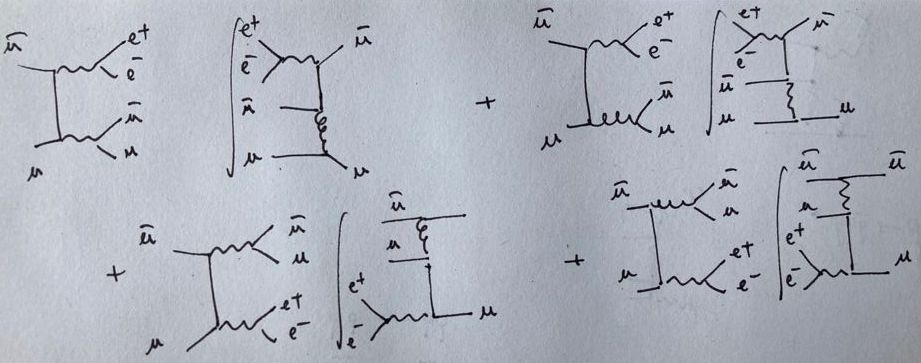
\includegraphics[width=\linewidth]{diagrams_qqbqqb_channel}
  \caption{Diagrams sample of divergent contribution to the $q  \barq \rightarrow l  \bar{l} + q  \barq$ process.}
  \label{fig:qbq_qbq}
\end{figure}
%%%%%%%%%%%%%
Here we present the extraction of the IR singularities relevant for the partonic process 
\beq
q(1) + \barq(2) \rightarrow l(3)+\bar{l}(4) + q(5) + \barq(6) \, .
\eeq  
{\color{orange}{code info}}: notation is chosen according to what is done for the numerical implementation. \\
This partonic cross section can only receives contributions from real radiation and from pdf 
renormalisation, according to
\beq
d\hat{\sigma}_{\rm nnlo}^{q\barq \rightarrow e^-e^+q\barq}
=
d\hat{\sigma}^{q\barq \rightarrow e^-e^+q\barq}_{\rm rr}
+d\hat{\sigma}^{q\barq \rightarrow e^-e^+q\barq}_{\rm pdf} \; ,
\eeq
where the double real term is 
\beq
2s\cdot d\hat{\sigma}_{rr}^{q\barq \rightarrow e^-e^+q\barq} 
\equiv 
\int[dp_5] [dp_6] \, F_{LM}(1_q,2_\barq,3_{e^-},4_{e^+} | 5_q, 6_{\bar{q}})  
\equiv 
\big\langle F_{LM}(1_q,2_\barq,3_{e^-},4_{e^+} | 5_q, 6_{\bar{q}})\big\rangle \, .
\nn
\eeq
Let us stress that such term (as well as the complete partonic cross section)
is not affected by soft singularities, and therefore only collinear subtraction
is actually needed. We begin by listing all the collinear singularities that may 
arise:
\beq
C_{56,1} \, , \quad
C_{56,2} \, .
\eeq
We stress that no strongly-ordered configurations may affect this partonic channel.
We then introduce a simple partition to separate the two triple-collinear regimes
\beq
1 = w^{51,61}+w^{52,62} = \frac{\eta_{52}}{\eta_{51}+\eta_{52}}
+
\frac{\eta_{51}}{\eta_{51}+\eta_{52}} \, , 
\eeq
such that
\beq
&&
C_{56,1} \,  w^{51,61} = C_{56,1} \, \frac{\eta_{52}}{\eta_{51}+\eta_{52}} = C_{56,1} \; , 
%\nn \\
%&&
%C_{16} \, C_{56,1} \,  w^{51,61} = C_{16} \, C_{56,1} \; , 
%\nn \\
%&&
%C_{15} \, C_{56,1} \,  w^{51,61} = C_{15} \, C_{56,1} \; ,
\nn  \\[6pt]
&&
C_{56,2} \,  w^{52,62} = C_{56,2} \, \frac{\eta_{51}}{\eta_{51}+\eta_{52}} = C_{56,2} \; , 
%\nn \\
%&&
%C_{26} \, C_{56,2} \,  w^{52,62} = C_{26} \, C_{56,2} \; , 
%\nn \\
%&&
%C_{25} \, C_{56,2} \,  w^{52,62} = C_{25} \, C_{56,2}  \; .
\eeq
As we have already mentioned, no strongly-ordered configurations appear.
However, to be able to use the well-know parametrisation of the triple-collinear
limits, we decide to introduce two subsectors. We emphasise that this choice is
purely guided by practical reasons.
We rewrite the identity as 
\beq
1 = w^{51,61}+w^{52,62} =  
w^{51,61} \, \big( \theta_A +\theta_C \big) 
+w^{52,62}\, \big( \theta_A +\theta_C \big) \; ,  
\eeq
where
\beq
\begin{cases}
{\rm sector \; A} : \quad \theta^{61} < \theta^{51} \, ,
\\
{\rm sector \; C} : \quad \theta^{51} < \theta^{61} \, .
\end{cases}
\eeq
(and analogous relations hold for sector $w^{52,62}$ up to substituting $1 \rightarrow 2$).
The limits enhanced in each sector are the following
\beq
\omega^{51,61} \, \theta_A  &:&  C_{61}, \, C_{56,1}
\nn \\[0.2cm]
&& 
\quad 
\rightarrow \; \omega^{51,61}  \, \theta_A  
=  \big[ C_{61} + C_{56,1} (1-C_{61}) + (1-C_{56,1})  (1-C_{61})  \big] \, \omega^{51,61}  \, \theta_A 
\nn \\
&&
\hspace{27mm}
=  \big[C_{56,1} + (1-C_{56,1})  \big] \, \omega^{51,61}  \, \theta_A 
\nn \\[0.2cm]
%%
\omega^{51,61} \, \theta_C  &:& C_{51}, \, C_{56,1}
\nn \\[0.2cm]
&& 
\quad
\rightarrow \; \omega^{51,61} \, \theta_C
=\big[ C_{51} + C_{56,1} (1-C_{51}) + (1-C_{56,1})  (1-C_{51})  \big] \,  \omega^{51,61} \, \theta_C
\nn \\
&&
\hspace{27mm}
=\big[ C_{56,1}+ (1-C_{56,1}) \big] \,  \omega^{51,61} \, \theta_C 
\nn \\[0.2cm]
%%
\omega^{52,62} \, \theta_A  &:&  C_{62}, \, C_{56,2}
\nn \\[0.2cm]
&& 
\quad 
\rightarrow \; \omega^{52,62}  \, \theta_A  
=  \big[ C_{62} + C_{56, 2} (1-C_{62}) + (1-C_{56,2})  (1-C_{62})  \big] \, \omega^{52,62}  \, \theta_A 
\nn \\
&&
\hspace{27mm}
= \big[ C_{56, 2} + (1-C_{56,2})  \big] \, \omega^{52,62}  \, \theta_A 
\nn \\[0.2cm]
%%
\omega^{52,62} \, \theta_C  &:& C_{52}, \, C_{56,2}
\nn \\[0.2cm]
&& 
\quad
\rightarrow \; \omega^{51,61} \, \theta_C
= \big[ C_{52} + C_{56,2} (1-C_{52}) + (1-C_{56,2})  (1-C_{52})  \big] \,  \omega^{52,62} \, \theta_C
\nn \\
&&
\hspace{27mm}
= \big[ C_{56,2} + (1-C_{56,2}) \big] \,  \omega^{52,62} \, \theta_C
\eeq
At this point we reorganise, as usual, the limits according to the
corresponding kinematics. We obtain
\beq
1 = \Omega^{\, q\barq} =
\Omega^{\, q\barq}_1
+ \Omega^{\, q\barq}_2   \; , 
\eeq 
with
\beq
\Omega^{\, q\barq}_1
&=&
(1-C_{56,1}) \, \omega^{51,61}  \, \theta_A 
+ (1-C_{56,1}) \, \omega^{51,61}  \, \theta_C
\nn \\
&&
+\, (1-C_{56,2}) \, \omega^{52,62}  \, \theta_A 
+ (1-C_{56,2}) \, \omega^{52,62}  \, \theta_C 
\label{eq:Omega1_qqb} \\
\Omega^{\, q\barq}_2
&=&
C_{56,1} \, \omega^{51,61}  \, \big(\theta_A+\theta_C \big) 
+
C_{56,2} \, \omega^{52,62}  \, \big(\theta_A+\theta_C \big) \; .
\label{eq:Omega2_qqb} 
\eeq
Let us stress that in Max's paper he has computed
\beq
C_{56,1} \, \omega^{51,61}  \, 
\Big[ 
\big( 1 - C_{61}\big) \, \theta_A
+ \big( 1 - C_{56}\big) \, \theta_B
+ \big( 1 - C_{51}\big) \, \theta_C
+ \big( 1 - C_{56}\big) \, \theta_D
\Big] \; .
\eeq
Since in our case all the single collinear limits are null, 
the it is sufficient to take Max's result and abelianize it.
The real matrix element can be then rewritten as
\beq
\big\langle F_{LM}(1_q,2_\barq,3_{e^-},4_{e^+} | 5_q, 6_{\bar{q}})\big\rangle
&=& 
\big\langle  \Omega^{\, q\barq} \, 
F_{LM}(1_q,2_\barq,3_{e^-},4_{e^+} | 5_q, 6_{\bar{q}})\big\rangle
\nn \\
&=&
\sum_{i=1}^2
\big\langle   \Omega^{\, q\barq}_i \, 
F_{LM}(1_q,2_\barq,3_{e^-},4_{e^+} | 5_q, 6_{\bar{q}})\big\rangle
\; .
\nn 
\eeq


\subsection{Real contribution}
Here we report the formulas relevant for the subtraction of the 
$q  \barq \rightarrow l  \bar{l} + q  \barq$ channel.

\subsubsection{Triple collinear}
We begin with the triple collinear limit, which can be borrowed from 
the results deduced in the NNLO QCD case. We have
\beq
 && \hspace{-7mm}
 \big\langle 
 \Omega^{q\barq}_2
\, F_{LM}(1_q,2_\barq,3_{e^-},4_{e^+} | 5_q, 6_{\bar{q}})
\big\rangle =
\nn \\
&&
=
\frac{ [\alpha_s] [\alpha] Q_q^2 \, C_F}{\eps} 
\int_0^1 dz \, 
\bigg[
 (2 E_1)^{-4\eps} 
P_{q\rightarrow q\barq q^*}^{TC}\big(z,E_1\big) \,
\Big\langle
\frac{F_{LM}(z\cdot1_q,2_\barq,3_{e^-},4_{e^+})}{z}
\Big\rangle
 \nn \\
 && \hspace{40mm}
+
 (2 E_2)^{-4\eps} 
P_{q\rightarrow q\barq q^*}^{TC}\big(z,E_2\big) \, 
\Big\langle
\frac{F_{LM}(1_q,z\cdot2_\barq,3_{e^-},4_{e^+} )}{z}
\Big\rangle
\bigg]
\, ,
\eeq
where $ P_{q\rightarrow q\barq q^*}^{TC}$ have to be deduced from Max's paper.
(\Chiara[CAVEAT: the result can be taken without modification
from Max's paper independently of the number of subsectors we 
introduce for the triple collinear sector. This is possible because
in the mixed QCD$\times$QED case the strongly ordered
limit vanish when acting on the squared matrix element.])

\subsection{PDFs contribution}
The PDFs contribution reads
\beq
2s \cdot d\hat{\sigma}^{q\barq \rightarrow e^-e^+q\barq}_{\rm pdf}
&=&
 [\alpha(\mu)] \, 
[\alpha_s(\mu)] \;
 \frac{Q_q^2\, C_F}{2 \eps}
\int_0^1 dz \, \bar{P}_{qq}^{\rm AP, \, 1}(z) \; \times
\nn \\
&& \quad \times \, 
\bigg[
\Big\langle
\frac{F_{LM}(z\cdot1_q,2_\barq,3_{e^-},4_{e^+})}{z}
\Big\rangle
+
\Big\langle
\frac{F_{LM}(1_q,z\cdot2_\barq,3_{e^-},4_{e^+} )}{z}
\Big\rangle
\bigg]
 \, ,
 \qquad
\eeq
where $ [\alpha(\mu)],
[\alpha_s(\mu)]$ are the renormalised coupling constants, and
$\bar{P}_{qq}^{\rm AP, \, 1}(z)$ can be obtained by taking
Eq.(4.107) and (4.119) in the {\it Pink Book} in their abelianized
versions, and subtracting Eq.(D2) of the {\it W-paper}. 
The reason is the following: in the literature the
splitting function is computed inclusively, i.e. by summing
$gg$ and $q\barq$ final states. 
Here we need the contribution of $q\barq$ final state only, 
therefore we have to subtract the terms corresponding to 
the $g g$ emission ($g \gamma$ after abalianization), 
which have already been identified for the
$W$-production. We have
\beq
\bar{P}_{qq}^{\rm AP, \, 1}(z)
&=&
- \Big( 2 \log z \, \log(1-z)
+ \frac32 \log z\Big)
\Big( \frac{2}{1-z}-1-z\Big)
- \Big(
\frac32
+\frac72 \,z \Big) \log z
\nn \\
&&
- \frac12 (1+z) \, \log^2z
-5(1-z)
-\bigg[
3
-2z
+ 2\Big( 1-\frac{1+z^2}{1-z}\log(1-z)\Big) \log z
\nn \\
&&
+ \frac{1+3z^2}{2(1-z)} \, \log^2z
+2 \, \frac{1+z^2}{1-z}
{\rm Li}_2(1-z)
\bigg] \; .
\eeq

\subsection{Analytic results for the fully differential calculation in the $q \barq \rightarrow q \barq$ channel}

Here we report the explicit expression of the finite reminder for the $q \barq \rightarrow Z \rightarrow e^+e^- q \barq$ cross-section.
The cancellation of the IR poles has been proven in the previous sections for a generic reference frame and without a specific choice for $E_{\rm max}$. 
However, to reduce the bookkeeping we present the finite remainder in the center-of-mass frame of the colliding partons, and setting  $E_{\rm max}=E_1=E_2\equiv E_c$. We decompose the cross-section into
\beq
2s\cdot d \sigma^{\rm QCD \otimes QED}_{q\barq \rightarrow e^-e^+q\barq}
=
2s\cdot d \sigma^{\rm boost}_{q\barq \rightarrow e^-e^+q\barq}
+
2s\cdot d \sigma^{\rm regulated}_{q\barq \rightarrow e^-e^+q\barq} \; .
\label{eq:xsect_qqb_into_qqb_decomp}
\eeq
The definitions of the different pieces are reported below\\
\Chiara[Warning: in the abelianisation procedure we need to substitute
$C_F^2$ with $2 C_F \, Q_q^2$!!!]
\beq
2s\cdot d \sigma^{\rm boost}_{q\barq \rightarrow e^-e^+q\barq}
&=&
 [\alpha(\mu)] \, 
[\alpha_s(\mu)] \,
\Chiara[2] \, Q_q^2\, C_F \, 
\int_0^1 dz \, 
P^{\rm NNLO}_{q\barq \rightarrow q\barq}(z)
\bigg[
\Big\langle
\frac{F_{LM}(z\cdot1_q,2_\barq,3_{e^-},4_{e^+} )}{z}
\Big\rangle
\nn \\
&& \hspace{50mm}
+
\Big\langle
\frac{F_{LM}(1_q,z\cdot2_\barq,3_{e^-},4_{e^+} )}{z}
\Big\rangle
\bigg] \; ,
\eeq
with
\beq
P^{\rm NNLO}_{q\barq \rightarrow q\barq}(z)
&=&
\frac{1+z^2}{1-z} \bigg[\log \Big(\frac{2 E_c}{\mu}\Big) \bigg(4 \text{Li}_2(z)-2 \log ^2(z)+4 \log (1-z) \log (z)-\frac{2 \pi ^2}{3}\bigg)
\nn \\
&&
+6 \text{Li}_3(1-z)
+8 \text{Li}_3(-z)
+9 \text{Li}_3(z)
+4 \text{Li}_2(z) \log (1-z)
   \nn \\
   &&
   -\log (z) \bigg(4 \text{Li}_2(-z)+3 \text{Li}_2(z)-4 \log ^2(1-z)+\frac{2 \pi ^2}{3}\bigg)
   \nn \\
   &&
   -\frac{7}{6} \log ^3(z)-\frac{1}{2} \log (1-z) \log
   ^2(z)-\frac{2}{3} \pi ^2 \log (1-z)\bigg]
   \nn \\
   &&
   +\bigg(\frac{(10-4 z^2) \log (z)}{z-1}
   +2 (7 z-8)\bigg) \log \Big(\frac{2 E_c}{\mu}\Big)
   +\frac{(z^2+6 z-13) \, \text{Li}_2(z)}{z-1}
   \nn \\
   &&
   +4 (z+1) \text{Li}_2(-z)
   +\frac{z^2 (6 \zeta_3+7)-6 z+6 \zeta_3-1}{2 (z-1)}
   +\frac{\pi ^2 \big(z^2-6 z+11\big)}{6 (z-1)}
   \nn \\
   &&
   -\frac{\big(4 z^2+12 z-25\big) \log
   ^2(z)}{4 (z-1)}
   +2 (7 z-8) \log (1-z)
   \nn \\
   &&
   -\Big(
   13 z^2
   -8 (z^2-1) \log (z+1)
   +19 z
   +6 (z-1)^2 \log (1-z)
   -22
   \Big) \, 
   \frac{ \log (z)}{2 (z-1)}
    \; .
    \nn\\
\eeq
Finally, we have defined
\beq
2s\cdot d \sigma^{\rm regulated}_{q\barq \rightarrow e^-e^+q\barq} 
=
\big\langle   \Omega^{\, q\barq}_2 \, 
F_{LM}(1_q,2_\barq,3_{e^-},4_{e^+} | 5_q, 6_{\bar{q}})\big\rangle \; ,
\eeq
where $\Omega^{\, q\barq}_2$ is introduced in Eq.\eqref{eq:Omega1_qqb}.


\section{The $q q \rightarrow q q$ channel}

\subsection{Introduction to the NNLO QCD$\times$QED subtraction for $q q \rightarrow q q$ channel}
 %%%%%%%%%%%figure%%%%%%%%%%
\begin{figure}
    \centering
    \begin{subfigure}{0.3\textwidth}
    \centering
        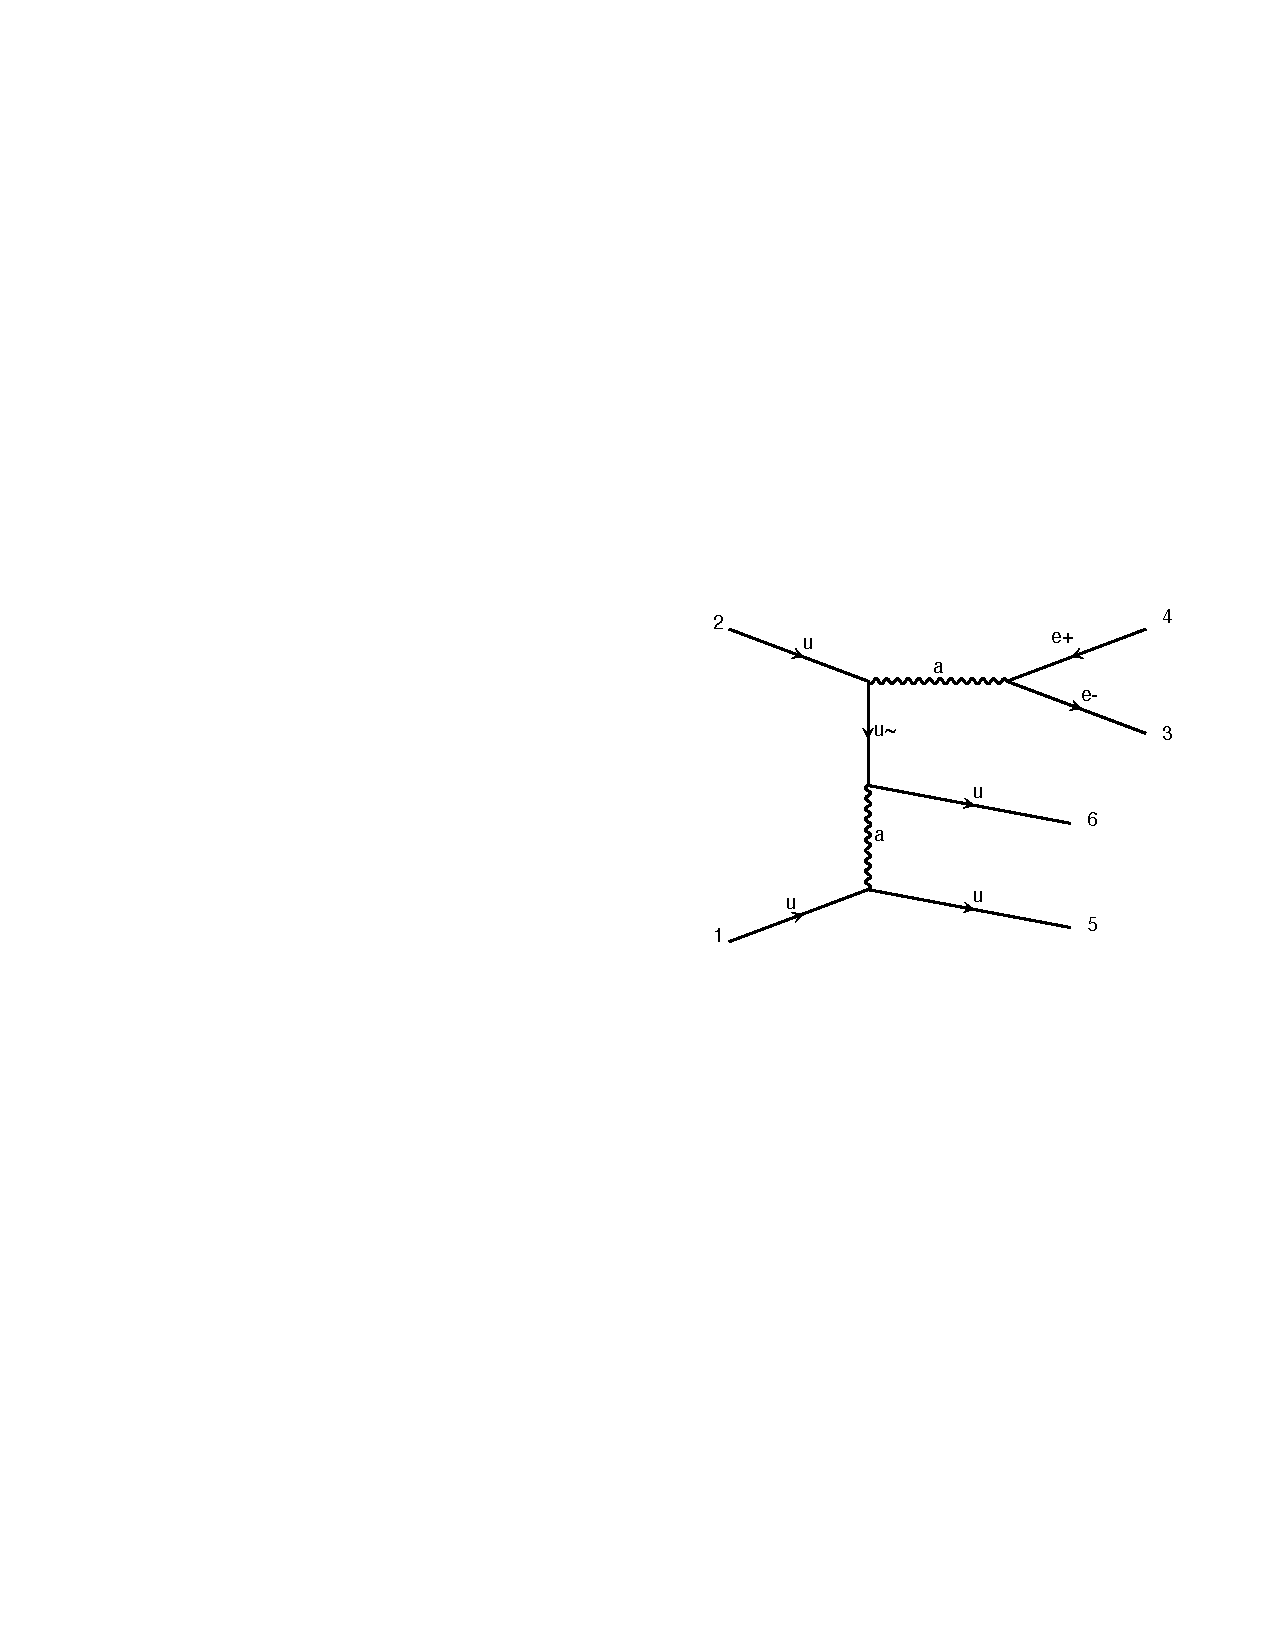
\includegraphics[width=\textwidth]{diagrams_qqqq_channel_a}
        \caption{}
        \label{fig:qqqq_a}
    \end{subfigure}
      \begin{subfigure}{0.3\textwidth}
      \centering
        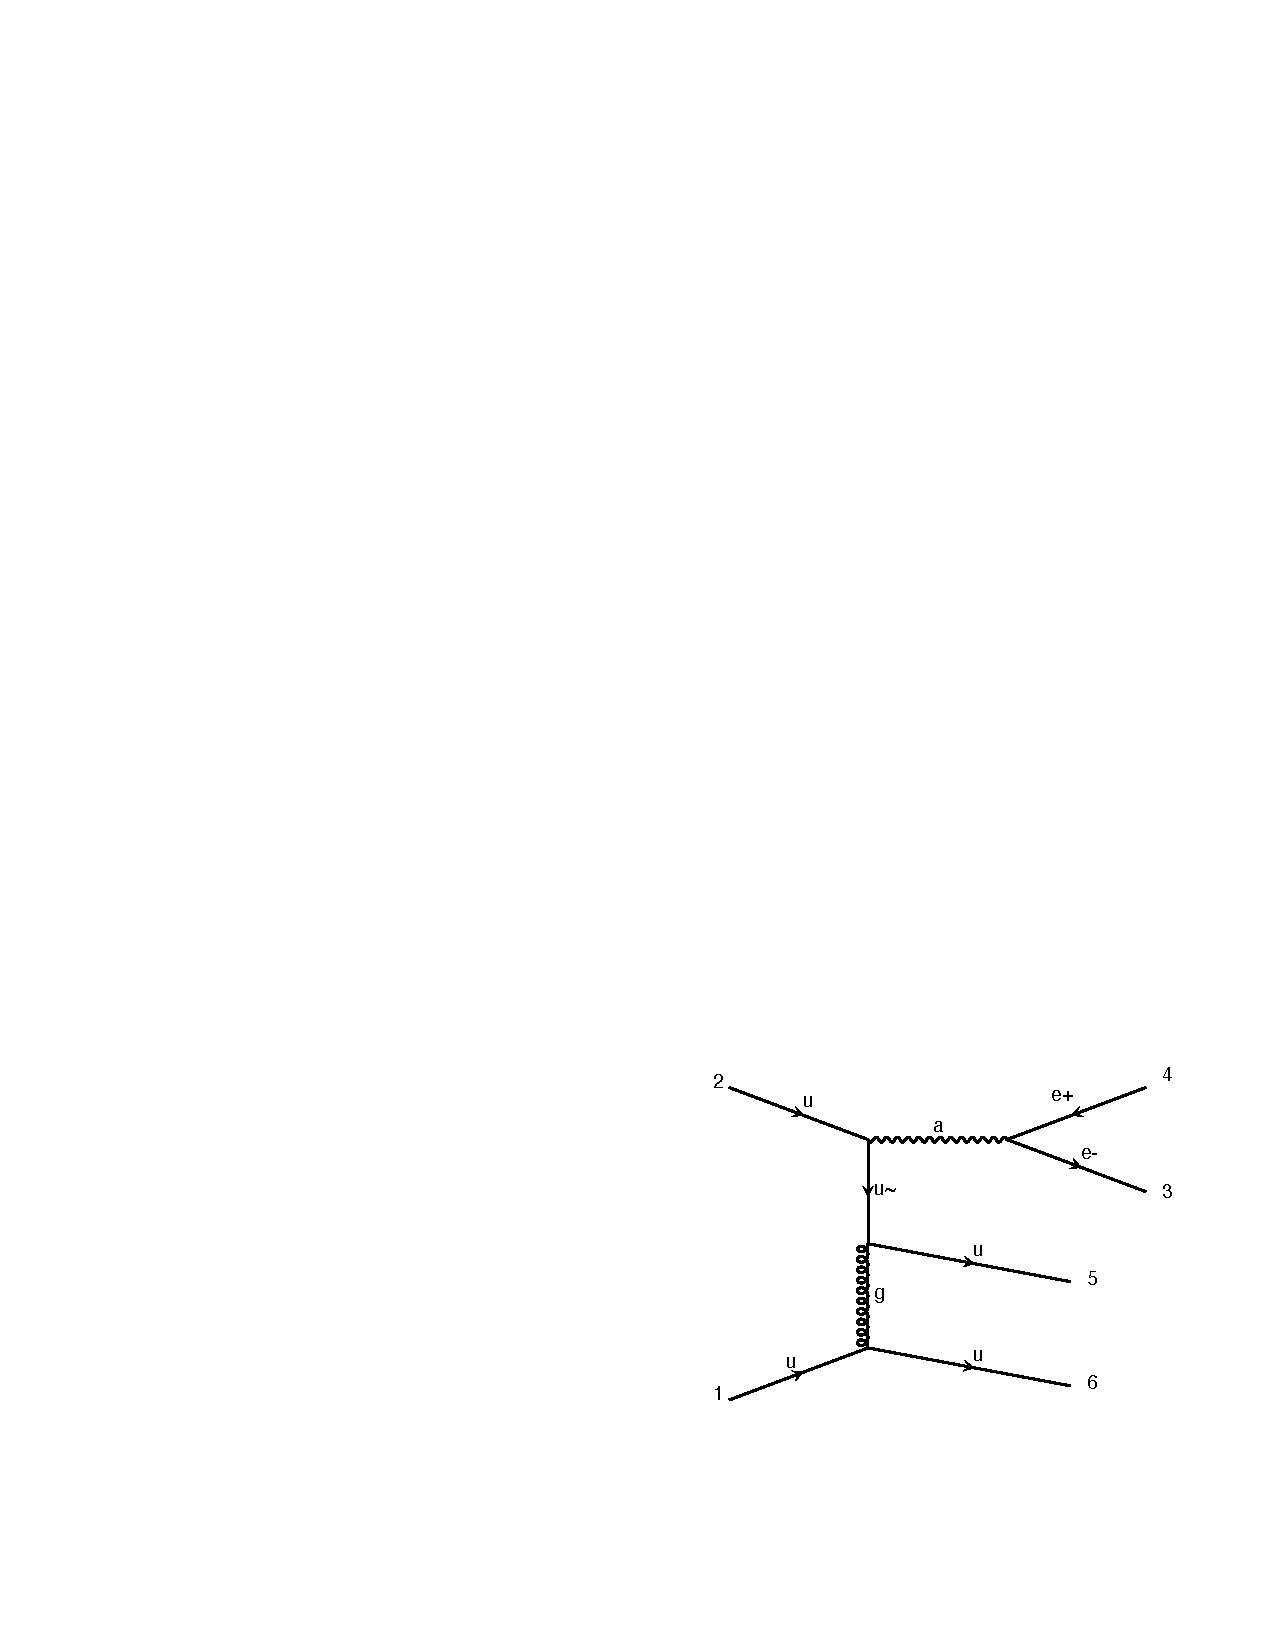
\includegraphics[width=\textwidth]{diagrams_qqqq_channel_b}
        \caption{}
        \label{fig:qqqq_b}
    \end{subfigure}
      \caption{Examples of Feynman graphs whose interference contributes to the NNLO correction for the $qq \rightarrow e^-e^+ qq$ channel.}
  \label{fig:nnlo_qqqq}
\end{figure}
%%%%%%%%%%%%%%%%%%%%%%

The entire structure of the IR subtraction can be borrowed 
from the $q \barq \rightarrow e^- e^+ q \barq$ channel.
We have
\beq
\big\langle F_{LM}(1_q,2_q,3_{e^-},4_{e^+} | 5_q, 6_q)\big\rangle
&=& 
\big\langle  \Omega^{\, qq} \, 
F_{LM}(1_q,2_q,3_{e^-},4_{e^+} | 5_q, 6_q)\big\rangle
\nn \\
&=&
\sum_{i=1}^2
\big\langle   \Omega^{\, qq}_i \, 
F_{LM}(1_q,2_q,3_{e^-},4_{e^+} | 5_q, 6_q)\big\rangle
\; ,
\eeq
where $\Omega^{\, qq}_i  =  \Omega^{\, q\barq}_i$, with the l.h.s.
given in Eq.\eqref{eq:Omega1_qqb} and Eq.\eqref{eq:Omega2_qqb}.

\subsubsection{Triple collinear}
We begin with the triple collinear limit, which can be borrowed from 
the results deduced in the NNLO QCD case. We have
\beq
 && \hspace{-7mm}
 \big\langle 
 \Omega^{qq}_2
\, F_{LM}(1_q,2_q,3_{e^-},4_{e^+} | 5_q, 6_{\bar{q}})
\big\rangle =
\nn \\
&&
=
\frac{ [\alpha_s] [\alpha] Q_q^2 \, C_F}{\eps} 
\int_0^1 dz \, 
\bigg[
 (2 E_1)^{-4\eps} 
P_{q\rightarrow qq \barq^*}^{TC}\big(z,E_1\big) \,
\Big\langle
\frac{F_{LM}(z\cdot1_\barq,2_q,3_{e^-},4_{e^+})}{z}
\Big\rangle
 \nn \\
 && \hspace{40mm}
+
 (2 E_2)^{-4\eps} 
P_{q\rightarrow qq \barq^*}^{TC}\big(z,E_2\big) \, 
\Big\langle
\frac{F_{LM}(1_q,z\cdot2_\barq,3_{e^-},4_{e^+} )}{z}
\Big\rangle
\bigg]
\, ,
\eeq
where $P_{q\rightarrow qq \barq^*}^{TC}$ have to be deduced from Max's paper.

\subsection{PDFs contribution}
The PDFs contribution is quite similar to the $q\barq \rightarrow q\barq$ channel.
We can then write
\beq
2s \cdot d\hat{\sigma}^{q\barq \rightarrow e^-e^+q\barq}_{\rm pdf}
&=&
 [\alpha(\mu)] \, 
[\alpha_s(\mu)] \;
 \frac{Q_q^2\, C_F}{2 \eps}
\int_0^1 dz \, \bar{P}_{q\barq}^{\rm AP, \, 1}(z) \; \times
\nn \\
&& \quad \times \, 
\bigg[
\Big\langle
\frac{F_{LM}(z\cdot1_\barq,2_q,3_{e^-},4_{e^+})}{z}
\Big\rangle
+
\Big\langle
\frac{F_{LM}(1_q,z\cdot2_\barq,3_{e^-},4_{e^+} )}{z}
\Big\rangle
\bigg]
 \, ,
 \qquad
\eeq
where $ [\alpha(\mu)],
[\alpha_s(\mu)]$ are the renormalised coupling constants, and
$\bar{P}_{q\barq}^{\rm AP, \, 1}(z)$ can be obtained by taking
Eq.(4.108) in the {\it Pink Book} in its abelianized
version. In this case there is no need to subtract 
Eq.(D2) of the {\it W-paper}, since there is no
contribution from $q\barq \rightarrow g\gamma$
that can interfere with $qq \rightarrow qq$. We have
\beq
\bar{P}_{q\barq}^{\rm AP, \, 1}(z)
&=&
2 \, \Big( \frac{2}{1+z}
- 1
+z
\Big)
\Big(
-2 {\rm Li}_2(-z)
+\frac12 \log^2 z
- 2 \log z \, \log (1+z)
- \frac{\pi^2}{6} 
\Big)
\nn \\
&&
+ \, 2 (1+z) \log z
+ 4 (1-z)
 \; .
\eeq

\subsection{Analytic results for the fully differential calculation in the 
$q q \rightarrow q q$ channel}

Here we report the explicit expression of the finite reminder for the 
$q q \rightarrow Z \rightarrow e^+e^- q q$ cross-section.
The cancellation of the IR poles has been proven in the previous sections for a generic reference frame and without a specific choice for $E_{\rm max}$. 
However, to reduce the bookkeeping we present the finite remainder in the center-of-mass frame of the colliding partons, and setting  $E_{\rm max}=E_1=E_2\equiv E_c$. We decompose the cross-section into
\beq
2s\cdot d \sigma^{\rm QCD \otimes QED}_{qq \rightarrow e^-e^+qq}
=
2s\cdot d \sigma^{\rm boost}_{qq \rightarrow e^-e^+qq}
+
2s\cdot d \sigma^{\rm regulated}_{qq \rightarrow e^-e^+qq} \; .
\label{eq:xsect_qqb_into_qqb_decomp}
\eeq
The definitions of the different pieces are reported below \\
\Chiara[Warning: in the abelianisation procedure we need to substitute
$C_F^2$ with $2 C_F \, Q_q^2$. Moreover, the symmetry factor 1/2
is already included in Max's results, and in the Pink Book expressions!!!]
\beq
2s\cdot d \sigma^{\rm boost}_{qq \rightarrow e^-e^+qq}
&=&
 [\alpha(\mu)] \, 
[\alpha_s(\mu)] \,
\Chiara[2] \, 
Q_q^2\, C_F \, 
\int_0^1 dz \, 
P^{\rm NNLO}_{qq \rightarrow qq}(z) \; \times
\nn \\
&&
\times \, 
\bigg[
\Big\langle
\frac{F_{LM}(z\cdot1_\barq,2_q,3_{e^-},4_{e^+})}{z}
\Big\rangle
+
\Big\langle
\frac{F_{LM}(1_q,z\cdot2_\barq,3_{e^-},4_{e^+} )}{z}
\Big\rangle
\bigg] \; ,
\eeq
with
\beq
P^{\rm NNLO}_{q\barq \rightarrow q\barq}(z)
&=&
\log \Big(\frac{2 E_c}{\mu }\Big) 
\bigg[
\frac{1+z^2}{1+z}
\bigg(-8 \text{Li}_2(-z)
+2 \log ^2(z)
-8 \log (z+1) \log (z)\bigg)
\nn \\
&& \qquad \qquad \qquad
-\frac{2 \pi ^2 \big(z^2+1\big)}{3(z+1)}
-8 (z-1)+4 (z+1) \log (z)\bigg]
\nn \\
&&
+\frac{1+z^2}{1+z} \bigg[
-4 \text{Li}_3(1-z^2)
+8 \text{Li}_3(1-z)
-18 \text{Li}_3(-z)
-8 \text{Li}_3(z)
\nn \\
&& \hspace{17mm}
-12 \text{Li}_3\Big(\frac{z}{z+1}\Big)
+\log (z) \Big(2 \text{Li}_2(-z)
+2 \text{Li}_2(z)
-6 \log ^2(z+1)\Big)
\nn \\
&&  \hspace{17mm}
-8\log (1-z) \Big(\text{Li}_2(-z)+\log (z) \log
   (z+1)\Big) 
   +\frac{7 \log ^3(z)}{6}
   \nn \\
   &&  \hspace{17mm}
   +2 \log ^3(z+1)
   -\log (z+1) \log ^2(z)
   -\pi ^2 \log (z+1)\bigg]  
   \nn \\
   &&
   -6 (z+1) \text{Li}_2(-z)
   -2 (z+3) \text{Li}_2(z)
   +\frac{5 (z^2+1) \zeta_3}{z+1}
   \nn \\
   &&
   +\bigg(\frac{2 \pi ^2 (z^2+1)}{3 (z+1)} 
   +\frac{1}{2} (11 z+19)
   -6 (z+1) \log (z+1)\bigg) \log (z)
   \nn \\
   &&
   -2\log (1-z)
   \bigg(\frac{\pi ^2 (z^2+1)}{3 (z+1)}
   +4 (z-1)
   - (z-1) \log (z)\bigg)
   \nn \\
   &&
   +\frac{1}{6} \pi ^2 (3-z)
   -\frac{15 (z-1)}{2}+2 (z+2) \log ^2(z)    \; .
    \nn\\
\eeq
Finally, we have defined
\beq
2s\cdot d \sigma^{\rm regulated}_{qq \rightarrow e^-e^+qq} 
=
\big\langle   \Omega^{\, qq}_2 \, 
F_{LM}(1_q,2_q,3_{e^-},4_{e^+} | 5_q, 6_q)\big\rangle \; ,
\eeq
where $\Omega^{\, qq}_2=\Omega^{\, q\barq}_2$ is introduced in Eq.\eqref{eq:Omega1_qqb}.
\newpage
\appendix

\section{Soft integral at NLO}

Here we compute the angular integral of the kinematic structure arising from the soft kernel. Ultimately, we want to prove the formula
\beq
\int [dp_k] \frac{\rho_{ij}}{E_k^2 \, \rho_{ik} \rho_{jk}}
= \frac{1}{\eps^2} (4 E_{\rm max}^2)^{-\eps} \frac{1}{8\pi^2} \frac{(4\pi)^\eps}{\Gamma(1-\eps)}
\frac{\Gamma^2(1-\eps)}{\Gamma(1-2\eps)} \, \eta_{ij} \, {}_2F_1 (1, 1, 1-\eps, 1-\eta_{ij}) \, .
\label{eq:soft_int_proof}
\eeq
In the r.h.s. of the equation above, the underlying angular integral 
\beq
I_{\Omega}
&=&
\int \frac{d\Omega^{(d-1)}}{2(2\pi)^{d-1}} \;  \frac{1}{\rho_{ik} \rho_{jk}} 
=
\int \frac{d\Omega^{(d-1)}}{2(2\pi)^{d-1}} 
\int_0^1 \frac{dx }{\big[x \rho_{ik} +(1-x)\rho_{jk}\big]^2}
=
\int \frac{d\Omega^{(d-1)}}{2(2\pi)^{d-1}} 
\int_0^1 \frac{dx}{\mathcal{D}^{2}} \, ,
\nn
\eeq
where we have introduced the denominator
\beq
\mathcal{D}
&=&
x \rho_{ik} +(1-x)\rho_{jk}
=
x(1-{n}_i\cdot n_k)
+(1-x)(1-n_{j} \cdot n_{k})
\nn \\
&=&
1-n_k \cdot (x \, n_i+(1-x) n_j)
=
1 -L_x  \, n_k\cdot n_x \, 
\eeq
with $n_x =[x n_i +(1-x) n_j]/L_x$. Requiring $n_x$ to be a unitary vector we can deduce $L_x$
\beq
n_x^2 = 1 
\quad
\Rightarrow 
\quad
L_x^2 = x^2 +(1-x)^2
+2x (1-x) n_i\cdot n_j
= 1-2x(1-x) \rho_{ij} \, .
\eeq
The phase space is parametrised by introducing $\cos\vartheta = n_k\cdot n_x$, such that
\beq
I_{\Omega}
&=&
\int \frac{d\Omega^{(d-2)}}{2(2\pi)^{d-1}} 
\int_0^1 dx
\int_{-1}^1 d\cos\vartheta \; \frac{(1-\cos^2\vartheta)^{-\eps}}{\big[1 -L_x  \, n_k\cdot n_x \big]^2} \; .
\eeq
A simple change of variable can be exploited to simply the integration, namely
\beq
\xi =  \frac{1+\cos\vartheta}{2} 
\; \rightarrow \; 
\cos\vartheta = 2\xi -1
\; \rightarrow \; 
d\cos\vartheta = 2 d\xi \, , 
\eeq
and get
\beq
I_{\Omega}
&=&
\frac{1}{8\pi^2} \, \frac{(4\pi)^\eps}{\Gamma(1-\eps)}
\int_0^1 dx \;
\frac{2^{1-2\eps}}{\big(1+L_x\big)^2}
\int_0^1 d\xi \, 
\xi^{-\eps} \, (1-\xi)^{-\eps} \, 
\Big(
1-\frac{2L_x}{1+L_x} \, \xi 
\Big)^{-2}
\nn \\
&=&
\frac{1}{8\pi^2} \, \frac{(4\pi)^\eps}{\Gamma(1-\eps)}
\int_0^1 dx \;
\frac{2^{1-2\eps}}{\big(1+L_x\big)^2} \; 
\frac{\Gamma^2(1-\eps)}{\Gamma(2-2\eps)} \;
{}_2F_{1}
\Big(2,1-\eps; 2-2\eps; \, 
\frac{2L_x}{1+L_x}  
\Big) \; .\qquad 
\eeq
To linearise the argument of the hypergeometric function we use the following property
\beq
{}_2F_{1}(a,b;2b; z)
= \left( 1-\frac z2\right)^{-a}
{}_2F_{1} \Big( 
\frac a2, 
\frac12+\frac a 2; 
b+\frac12;
\frac{z^2}{(2-z)^{2}}\Big) \, .
\eeq
In our case it easy to verify that 
\beq
\frac{z^2}{(2-z)^{2}} = L_x^2 = 1-2x(1-x) \, \rho_{ij}\; ,
\eeq
and then 
\beq
I_{\Omega}
&=&
\frac{1}{8\pi^2} \, \frac{(4\pi)^\eps}{\Gamma(1-\eps)}
\int_0^1 dx \;
\frac{2^{1-2\eps}}{\big(1+L_x\big)^2} \; 
\frac{\Gamma^2(1-\eps)}{\Gamma(2-2\eps)} \;
\Big(
\frac{1}{1+L_x}
\Big)^{-2}
{}_2F_{1}
\Big(1,\frac32; \frac32-\eps; \, 
L_x^2  
\Big)
\nn \\
&=&
2^{1-2\eps} 
\frac{1}{8\pi^2} \, \frac{(4\pi)^\eps}{\Gamma(1-\eps)} \, 
\frac{\Gamma^2(1-\eps)}{\Gamma(2-2\eps)} 
\int_0^1 dx \, 
{}_2F_{1}
\Big(1,\frac32; \frac32-\eps; \, 
L_x^2  
\Big)
 \; .
\eeq
To integrate the hypergeometric function it is convenient to use its Mellin-Barns representation
\beq
{}_2F_{1}(a,b;c; z) 
&=&
\frac{\Gamma(c)}{\Gamma(a) \, \Gamma(b) \, \Gamma(c-a) \, \Gamma(c-b)} \, \times
\nn \\
&& \times \, 
\frac1{2\pi i} \int_{-i\infty}^{i \infty}
dt \, \Gamma(a+t) \, \Gamma(b+t) \, \Gamma(c-a-b-t) \, \Gamma(-t) \, (1-z)^t \; ,
\quad 
\eeq
and obtain 
\beq
I_{\Omega}
&=&
2^{1-2\eps} 
\frac{1}{8\pi^2} \, \frac{(4\pi)^\eps}{\Gamma(1-\eps)} \, 
\frac{\Gamma^2(1-\eps)}{\Gamma(2-2\eps)}  \, 
\frac{\Gamma\left(\frac32-\eps\right)}{\Gamma\left(\frac32\right) \, \Gamma\left(\frac12-\eps\right) \, \Gamma(-\eps)}\times
\nn \\
&& 
\times
\int_0^1 dx \; 
\frac1{2\pi i} \int_{-i\infty}^{i \infty}
dt \, 
\big[x(1-x)\big]^t \, 
\big(2\rho_{ij}\big)^t \, 
\Gamma(1+t) \, 
\Gamma\Big(\frac32+t\Big) \, 
\Gamma(-\eps-1-t) \, 
\Gamma(-t)
\nn \\
&=&
2^{-2\eps} 
\frac{1}{8\pi^2} \, \frac{(4\pi)^\eps}{\Gamma(1-\eps)} \, 
\frac{\Gamma^2(1-\eps)}{\Gamma(2-2\eps)}  \, 
\frac{ \sqrt{\pi}  \, \Gamma\left(\frac32-\eps\right)}{\Gamma\left(\frac32\right) \, \Gamma\left(\frac12-\eps\right) \, \Gamma(-\eps)}\times
\nn \\
&& 
\times
\frac1{2\pi i} \int_{-i\infty}^{i \infty}
dt \, 
\Gamma(1+t)  \, 
\Gamma(1+t)
\Gamma(-\eps-1-t) \, 
\Gamma(-t) \, 
\Big(\frac{\rho_{ij}}{2}\Big)^t \, 
 \; ,
\eeq
where in the last step we have integrated over $x$ using
\beq
\int_0^1 dx \;  
\big[x(1-x)\big]^t = \frac{\Gamma^2(1+t)}{\Gamma(2+2t)}
=
\frac{2^{-1-2t} \sqrt{\pi} \, \Gamma(1+t)}{\Gamma\left(\frac32+t\right)} \; .
\eeq
At this point we transform back the Mellin-Barns representation and get
\beq
I_{\Omega}
&=&
2^{-2\eps} 
\frac{1}{8\pi^2} \, \frac{(4\pi)^\eps}{\Gamma(1-\eps)} \, 
\frac{\Gamma^2(1-\eps)}{\Gamma(2-2\eps)}  \, 
\frac{ \sqrt{\pi}  \, \Gamma\left(\frac32-\eps\right)}{\Gamma\left(\frac32\right) \, \Gamma\left(\frac12-\eps\right)} \, 
\frac{\Gamma(-\eps)}{\Gamma(1-\eps)} \; 
{}_2F_{1}
\Big(1,1; 1-\eps; \, 
1-\eta_{ij}
\Big) 
\nn \\
&=&
-
\frac{2^{-2\eps}}{\eps} 
\frac{1}{8\pi^2} \, \frac{(4\pi)^\eps}{\Gamma(1-\eps)} \, 
\frac{\Gamma^2(1-\eps)}{\Gamma(1-2\eps)}  \; 
{}_2F_{1}
\Big(1,1; 1-\eps; \, 
1-\eta_{ij}
\Big) 
 \; .
 \label{eq:angular_integral}
\eeq
To complete our calculation it is sufficient to include the integration over the ratiation energy 
\beq
\int [dp_k] \frac{\rho_{ij}}{E_k^2 \, \rho_{ik} \rho_{jk}}
&=&
\int_0^{E_{\rm max}} \frac{dE_k}{E_k^{1+2\eps}} \,
\int \frac{d\Omega^{(d-1)}}{2(2\pi)^{d-1}} 
\frac{1}{\rho_{ik} \rho_{jk}} \, \rho_{ij}
\nn \\
&=&
\frac{1}{2\eps} \, E_{\rm max}^{-2\eps} \;
\rho_{ij}
\bigg[
\frac{2^{-2\eps}}{\eps} 
\frac{1}{8\pi^2} \, \frac{(4\pi)^\eps}{\Gamma(1-\eps)} \, 
\frac{\Gamma^2(1-\eps)}{\Gamma(1-2\eps)}  \; 
{}_2F_{1}
\Big(1,1; 1-\eps; \, 
1-\eta_{ij}
\Big) 
\bigg]
\nn \\
&=&
\frac{1}{\eps^2} \, (2E_{\rm max})^{-2\eps} \;
\frac{1}{8\pi^2} \, \frac{(4\pi)^\eps}{\Gamma(1-\eps)} \, 
\frac{\Gamma^2(1-\eps)}{\Gamma(1-2\eps)}  \; 
\eta_{ij} \; 
{}_2F_{1}
\Big(1,1; 1-\eps; \, 
1-\eta_{ij}
\Big) \, ,
\nn
\eeq
and verify that we have precisely obtained Eq.\eqref{eq:soft_int_proof}. \\
It is evident that the most complicated part of
the computation relays on the evaluation of the 
angular integral 
\beq
I_{\Omega}
=
\int \frac{d\Omega^{(d-1)}}{2(2\pi)^{d-1}} \;  \frac{1}{\rho_{ik} \rho_{jk}} \; .
\eeq
In the previous paragraphs we have presented
how $I_{\Omega}$ can be evaluated by means 
of Feynman parameters. Although such a technique
is quite powerful, it is also clear that it is hard to 
generalised to more complicated integrand and 
multi-particle phase space. Let's just think to the 
2-parton soft current, which we need to integrate
over a double unresolved phase space.
In view of tackling NNLO complexity integrals, we
need to adopt a more sophisticated procedure
to face phase space integrals. One interesting
option is known as {\it reverse unitarity}.
The crucial idea is to map phase space integrals
into loop integrals and exploit the well known 
machinery has already been developed by the 
amplitude community.
In the next lines we will find the result in Eq.
\eqref{eq:angular_integral} by solving a one-loop
integral. 
We will first recall some important concepts that
will come at hand at a second time. \\
We introduce the $\delta$ functions
\beq
&&
\delta^+(k^2) 
= \delta^+\big( k_0^2-\vec{k}^2\big) 
= \frac{\delta \big( k_0-|\vec{k}| \big)}{2 k_0} \; ,
\nn \\
&&
\delta \big( (k-P)^2\big) 
= \delta \big( s-2\sqrt{s} \, k_0 \big)
= \frac{\delta \big( \sqrt{s}/2-k_0\big)}{2 \sqrt{s}} \; ,
\eeq
where we have defined $P = \big( \sqrt{s}, \vec{0}\big)$.
Moreover, given the relation
\beq
d^{d-1} \vec{k} 
= |\vec{k}|^{d-2} \, d|\vec{k}| \, d \Omega_k^{(d-1)}
\eeq
we prove a key identity
\beq
\int d^d k \, \delta^{+}(k^2) \, \delta \big( (k-P)^2\big) 
&=&
\int d k_0 \, d^{d-1} {\vec k} \,  \frac{\delta \big( k_0-|\vec{k}| \big)}{2 k_0}
\,  \frac{\delta \big( \sqrt{s}/2-k_0\big)}{2 \sqrt{s}}
\nn \\
&=&
\int  d^{d-1} {\vec k} \,  \frac{\delta \big( \sqrt{s}/2-|\vec{k}| \big)}{ 2s}
\nn \\
&=&
\int d |\vec{k}| \, |\vec{k}|^{d-2} \, d\Omega^{(d-1)}_k
 \,  \frac{\delta \big( \sqrt{s}/2-|\vec{k}| \big)}{ 2s}
 \nn \\
 &=&
 \int d\Omega^{(d-1)}_k
 \,  \frac{(\sqrt{s}/2)^{d-2}}{ 2s}
 \nn \\
 &=&
\frac{s^{\frac{d-2}{2}-1}}{2^{d-2+1}}
  \int d\Omega^{(d-1)}_k
  =
  \frac12 \; 
  s^{-\eps} \, 4^{-1+\eps}
  \int d\Omega^{(d-1)}_k \, ,
\eeq
and then
\beq
&&
2 \,   s^{\eps} \, 4^{1-\eps} \; 
d^d k \,  \delta^{+}(k^2) \, \delta \big( (k-P)^2\big) 
  =
d\Omega^{(d-1)}_k
\nn \\
&& \qquad
\rightarrow 
\;
\frac{d\Omega^{(d-1)}}{2(2\pi)^{d-1}}
=
\frac{s^{\eps} \, 4^{1-\eps}}{(2\pi)^{d-1}} \;  
d^d k \,  \delta^{+}(k^2) \, \delta \big( (k-P)^2\big) \; .
\label{eq:PS_to_Loop_identity}
\eeq
As a further step, we recall that the imaginary 
part of a loop amplitude arises from virtual particles
that go on shell. In other words, Feynman propagators
develops imaginary parts if and only if $k^2 = M^2$
\beq
\Im \, \bigg[ \frac{1}{k^2-M^2 +i \eta}\bigg]
= 
\frac{1}{2 i}
\bigg(
\frac{1}{k^2-M^2 +i \eta}
-
\frac{1}{k^2-M^2 - i \eta}
\bigg)
=
- \frac{\eta}{(k^2-M^2)^2+\eta^2} \; , 
\eeq
upon integrating the r.h.s. we have
\beq
\lim_{\eta \rightarrow 0^+} 
\int_0^\infty dk^2 \; 
\frac{-\eta}{(k^2-M^2)^2+\eta^2}
&=&
\lim_{\eta \rightarrow 0^+} 
\int_0^\infty dk^2 \; 
\frac{-\eta}{\eta^2 \big[(\frac{k^2-M^2}{\eta})^2+1\big]}
\nn \\
&=&
-
\lim_{\eta \rightarrow 0^+} 
\int_{-\frac{M^2}{\eta}}^\infty  \; 
\frac{du}{u^2+1}
\nn \\
&=&
-
\lim_{\eta \rightarrow 0^+} 
\arctan(x) \bigg|_{-\frac{M^2}{\eta}}^\infty  
\nn \\
&=&
-\frac \pi2
+
\lim_{\eta \rightarrow 0^+} 
\arctan\Big(\frac{-M^2}{\eta}\Big) 
\nn \\
&=&
- \pi
\nn \\
&=&
- \pi \int_0^\infty dk^2 \, 
\delta^+ \big( k^2-M^2\big) \; .
\eeq
As a result, we can relate $\delta$-functions in loop
integrals to the imaginary parts of loop integrals
where these $\delta$-functions are replaced by 
propagators. Such a procedure is formulated in the 
Cutosky rules
\beq
- \pi \, \delta^+ \big( p^2-M^2\big)
\; 
\leftrightarrow 
\;
\Im \, \bigg[ \frac{1}{k^2-M^2 +i \eta}\bigg] \; .
\label{eq:cutosky_rules}
\eeq
With all these informations at hand we can now 
proceed with the actual computation.
\beq
I_{\Omega}
&=&
\int \frac{d\Omega^{(d-1)}}{2(2\pi)^{d-1}} \;  \frac{1}{\rho_{ik} \rho_{jk}} 
\nn \\
&\overset{\rm Eq.\eqref{eq:PS_to_Loop_identity}}{=}&
\frac{s^{\eps} \, 4^{1-\eps}}{(2\pi)^{d-1}} 
\int  
d^d k \,  \delta^{+}(k^2) \, \delta \big( (k-P)^2\big)
\;  \frac{1}{\rho_{ik} \rho_{jk}} 
\nn \\
&=&
\frac{s^{\eps} \, 4^{1-\eps}}{(2\pi)^{d-1}} 
\int  
d^d k \,  \delta^{+}(k^2) \, \delta \big( (k-P)^2\big)
\;  \frac{E_i \, E_j \, E_k^2}{p_i \cdot k \, p_j \cdot k} 
\nn \\
&=&
\frac{s^{\eps} \, 4^{1-\eps}}{(2\pi)^{d-1}} 
\int  
d^d k \,  \delta^{+}(k^2) \, \delta \big( (k-P)^2\big)
\;  \frac{s^2/4}{(2p_i \cdot k) \, (2 p_j \cdot k)} 
\nn \\
&=&
\frac{s^{\eps+2} \, 4^{-\eps}}{(2\pi)^{d-1}} 
\int  
d^d k \;  
\frac{\delta^{+}(k^2) \, \delta \big( (k-P)^2\big)}{\big(k-p_i \big)^2 \, \big(k- p_j \big)^2} 
\nn \\
&\overset{\rm Eq.\eqref{eq:cutosky_rules}}{=}&
\frac{s^{\eps+2} \, 4^{-\eps}}{(2\pi)^{d-1}} \; 
\Im 
\bigg[
-i (2\pi i)^2
\int \frac{d^dk}
{\big[k^2 +i 0 \big] \, 
\big[ \big( k-p_i\big)^2 \big] \,
\big[ \big( k-p_j\big)^2 \big]\, 
\big[ (k-P)^2+i 0\big]}
\bigg]
\; .
\eeq
\Chiara[not sure about the prefactors in squared brackets!!!] \\
where we have introduced massless momenta 
$p_i= \sqrt{s}/2 \, \big( 1, \vec{n}_i\big)$.
At this point, the problem has been reduced to
evaluating a standard loop integral.
We can introduce Feynman parameters 
according to the formula
\beq
\frac{1}{A_1^{m_1} \, \dots \, A_n^{m_n}}
= \frac{\Gamma(M)}{\prod_{i=1}^n \Gamma(m_i)}
\int_0^1 dx_1 \dots
\int_0^1 dx_n \, 
\delta(1-X) \, 
\prod_{i=1}^n
x_i^{m_i-1} \, 
\bigg[ 
\sum_{i=1}^n x_i \, A_i \bigg]^{-M} \; , 
\eeq
with 
\beq
M = \sum_{i=1}^n m_i \; , 
\qquad
X = \sum_{i=1}^n x_i \; .
\eeq
This way we have
\beq
&&
\int \frac{d^dk}
{\big[k^2 +i 0 \big] \, 
\big( k-p_i\big)^2 \,
\big( k-p_j\big)^2 \, 
\big[ (k-P)^2+i 0\big]} =
\nn \\
&&
=
6 \int_0^1 dx \, dy \, dz \, 
z (1-z)
\int \frac{d^dk}
{\big[k^2 +i 0 -2 k\cdot \tilde{p}(x,y,z)
+z(1-x) \, s
\big]^4 } \, ,
\eeq
where the auxiliary momentum reads
\beq
 \tilde{p}^\mu(x,y,z)
 =
 (1-z)y \, p_i^\mu
 +z \big( x \, p_j^\mu +(1-x) \, P^\mu \big) \; .
\eeq
To solve the integral above we firs reabsorb 
the $i0$ prescription by the replacement
\beq
s \rightarrow s- i 0 \; ,
\eeq
 and then we complete the square in $k$ and shift the loop 
 momentum accordingly. We obtain
 \beq
 \int \frac{d^dk}
{\big[k^2 +i 0 -2 k\cdot \tilde{p}(x,y,z)
+z(1-x) \, s
\big]^4 }
=
 \int \frac{d^d\tilde{k}}
{\big[\tilde{k}^2
-\Delta\big]^4 } \; , 
 \eeq
 where
 \beq
 \tilde{k}^\mu &=& k^\mu-\tilde{p}^\mu \; , 
\nn \\
 \Delta &=& \tilde{p}^2 - z(1-x)\, s 
 = -z(1-z) \, 
 \Big[
 (1-x) \,  (1-y) \, s 
 -  x y \, (p_i+  p_j)^2 
 \Big]
 \nn \\
 &=&
  -z(1-z) \, 
 \Big[
 (1-x) \,  (1-y) \, s 
 +  x y \, t
 \Big] \, , 
 \eeq
 with $t =(p_i-p_j)^2$. The integrand function is now in a form suitable
 for direct integration by means of the well-known formula 
 \beq
 \int \frac{d^d \ell}{(2 \pi)^d} \; \frac{1}{\left[ \ell^2-\Delta \right] ^n} = \frac{(-1)^n i}{(4 \pi)^{d/2}} \, \frac{\Gamma(n-d/2)}{\Gamma(n)} \, \left( \frac{1}{\Delta} \right)^{n-d/2} \; .
 \label{scalar_mom_int}
\eeq
This way we have
\beq
\int \frac{d^dk}
{\big[k^2 +i 0 -2 k\cdot \tilde{p}(x,y,z)
+z(1-x) \, s
\big]^4 }
=
(2 \pi)^d
\frac{i}{(4 \pi)^{d/2}} \, \frac{\Gamma(2+\eps)}{6} \, \left( \frac{1}{\Delta} \right)^{2+\eps} 
\eeq
and then
\beq
&&
\int \frac{d^dk}
{\big[k^2 +i 0 \big] \, 
\big( k-p_i\big)^2 \,
\big( k-p_j\big)^2 \, 
\big[ (k-P)^2+i 0\big]} =
\nn \\
&&
=
6 (2 \pi)^d
\frac{i}{(4 \pi)^{d/2}} \, \frac{\Gamma(2+\eps)}{6} \,
\int_0^1 dx \, dy \, dz \, 
z (1-z)
 \left( \frac{1}{\Delta} \right)^{2+\eps}
 \nn \\
 &&
 =
 (2 \pi)^{d/2} \; 
\frac{i  \, \Gamma(2+\eps)}{2^{d/2}} \,
\int_0^1 dx \, dy \, dz \, 
\frac{\big[z (1-z)\big]^{-1-\eps}}{ \Big[ -
 (1-x) \,  (1-y) \, s 
 -  x y \, t
 \Big]^{2+\eps}}
  \nn \\
 &&
 =
 - \frac2\eps \, \frac{\Gamma^2(1-\eps)}{\Gamma(1-2\eps)}
 (2 \pi)^{d/2} \; 
\frac{i  \, \Gamma(2+\eps)}{2^{d/2}} \,
\int_0^1 dx \, dy \, 
\frac{1}{ \Big[ -
 (1-x) \,  (1-y) \, s 
 -  x y \, t
 \Big]^{2+\eps}}
 \nn \\
 &&
 =
 - \frac2{\eps(\epsilon +1)} \, \frac{\Gamma^2(1-\eps)}{\Gamma(1-2\eps)}
 (2 \pi)^{d/2} \; 
\frac{i  \, \Gamma(2+\eps)}{2^{d/2}} \,
\int_0^1 dx \, 
\bigg[
\frac{(-s (1-x))^{-\epsilon -1}-(-t x)^{-\epsilon -1}}{ s (1-x)- x \, t }
\bigg]
\nn \\
&&
 =
 - \frac2{\eps^2 \, (\epsilon +1)} \, \frac{\Gamma^2(1-\eps)}{\Gamma(1-2\eps)}
 (2 \pi)^{d/2} \; 
\frac{i  \, \Gamma(2+\eps)}{2^{d/2}} \, s^{-1}\times
\nn \\
&& \qquad 
\times
\bigg\{
(-s)^{-1-\eps} \, {}_2F_1\Big(1, 1, 1-\eps, 1+\frac{t}{s}\Big)
+
(-t)^{-1-\eps} \, {}_2F_1\Big(1, -\eps, 1-\eps, 1+\frac{t}{s}\Big)
\bigg\}
  \, .
\eeq
Finally we have
\beq
I_{\Omega}
&=&
\int \frac{d\Omega^{(d-1)}}{2(2\pi)^{d-1}} \;  \frac{1}{\rho_{ik} \rho_{jk}} 
\nn \\
&=&
\frac{s^{\eps+2} \, 4^{-\eps}}{(2\pi)^{d-1}} \; 
\Im 
\bigg[
i (2\pi)^2
\int \frac{d^dk}
{\big[k^2 +i 0 \big] \, 
\big[ \big( k-p_i\big)^2 \big] \,
\big[ \big( k-p_j\big)^2 \big]\, 
\big[ (k-P)^2+i 0\big]}
\bigg]
\nn \\
&=&
\frac{s^{\eps+2} \, 4^{-\eps}}{(2\pi)^{d-1}} \; 
\Im 
\bigg[
 (2\pi)^2 \, 
\frac2{\eps^2 \, (\epsilon +1)} \, \frac{\Gamma^2(1-\eps)}{\Gamma(1-2\eps)}
 (2 \pi)^{d/2} \; 
\frac{\Gamma(2+\eps)}{2^{d/2}} \, s^{-1}\times
\nn \\
&& \qquad 
\times
\bigg\{
(-s)^{-1-\eps} \, {}_2F_1\Big(1, 1, 1-\eps, 1+\frac{t}{s}\Big)
+
(-t)^{-1-\eps} \, {}_2F_1\Big(1, -\eps, 1-\eps, 1+\frac{t}{s}\Big)
\bigg\}
\bigg]
\; .
\eeq
We then notice that the factor $(-t)^{-1-\eps}$ as well as the hypergeometric functions are real. Moreover we use that
\beq
\Im \, \big[
-s +i 0
\big]^{-1-\eps} = -s^{-1-\eps} \, \sin(\pi \eps)
=
\frac{- \eps \, \pi \, s^{-1-\eps}}{\Gamma(1-\eps) \, \Gamma(1+\eps)} \, 
\eeq 
to write
\beq
I_{\Omega}
&=&
\int \frac{d\Omega^{(d-1)}}{2(2\pi)^{d-1}} \;  \frac{1}{\rho_{ik} \rho_{jk}} 
\nn \\
&=&
\frac{s^{\eps+2} \, 4^{-\eps}}{(2\pi)^{d-1}} \; 
 (2\pi)^2 \, 
\frac2{\eps^2 \, (\epsilon +1)} \, \frac{\Gamma^2(1-\eps)}{\Gamma(1-2\eps)}
 (2 \pi)^{d/2} \; 
\frac{\Gamma(2+\eps)}{2^{d/2}} \, s^{-1}\times
\nn \\
&& \qquad 
\times
\bigg\{
\frac{- \eps \, \pi \, s^{-1-\eps}}{\Gamma(1-\eps) \, \Gamma(1+\eps)} \, {}_2F_1\Big(1, 1, 1-\eps, 1+\frac{t}{s}\Big)
\bigg\}
\nn \\
&=&
- \frac{2^{-2\eps}}\eps \; 
\frac{(4 \pi)^{\eps}}{\Gamma(1-\eps)} \, 
 \frac{\Gamma^2(1-\eps)}{\Gamma(1-2\eps)} \; 
 {}_2F_1\Big(1, 1, 1-\eps, 1+\frac{t}{s}\Big)
\Chiara[\pi^{2}] 
\; .
\eeq
\Chiara[factor $\pi^2$ off!!!]


 
\section{Exercise on convolutions}


\section{Comments on abelianisation}

\subsection{double-virtual}

Also for the double virtual we can deduced (at least in the approximation of pure initial state corrections) the mixed QCD$\times$QED correction from the corresponding QCD$^2$ result.
We then assume to have two virtual gluons connecting the incoming quarks, and write the amplitude as
\beq
\mathcal{M}(1,2) = \mathcal{M}_0(1,2)
+ \frac{\alpha_s(\mu)}{2\pi} \, \mathcal{M}_1(1,2)
+ \Big( \frac{\alpha_s(\mu)}{2\pi} \Big)^2\, \mathcal{M}_2(1,2)  \, .
\eeq
The infrared structure of the one-loop and two-loop correction is known ad reads
\beq
\mathcal{M}_1(1,2) &=& \mathcal{I}_1(\epsilon) \, \mathcal{M}_0(1,2) + \mathcal{M}_{1, \rm fin }(1,2)
 \\
\mathcal{M}_2(1,2) &=& \mathcal{I}_2(\epsilon) \, \mathcal{M}_0(1,2) 
+ \mathcal{I}_1(\epsilon) \, \mathcal{M}_1(1,2)
+ \mathcal{M}_{2, \rm fin }(1,2) 
\nn \\
&=&
\Big( \mathcal{I}_2(\epsilon)+ \mathcal{I}_1^2(\epsilon) \Big)  \, \mathcal{M}_0(1,2) 
+ \mathcal{I}_1(\epsilon) \, \mathcal{M}_{1, \rm fin}(1,2)
+ \mathcal{M}_{2, \rm fin }(1,2)  \; ,
\eeq
where the soft current $\mathcal{I}_1$ has been introduced in Eq. \eqref{eq:soft_virtual_current_qcd}. We report it here for later convenience
\beq
\mathcal{I}_1(\epsilon)
 &=&-2C_F \, 
 \frac12 \, \frac{e^{\epsilon \gamma_E}}{\Gamma(1-\epsilon)} \; 
 \Big( \frac1{\epsilon^2} + \frac32 \, \frac1\epsilon \Big) \; 
  \Big( \frac{\mu^2 }{s_{12}} \Big)^\epsilon \;  
e^{-i \pi \epsilon} \; .
 \label{eq:I1}
\eeq
Moreover, the two-loop soft current is given by
\beq
\mathcal{I}_2(\epsilon) = 
-\frac12 \, \mathcal{I}_1(\epsilon) \Big(\mathcal{I}_1(\epsilon)+\frac{2\beta_0}{\epsilon} \Big)
+  \frac{e^{- \epsilon \gamma_E}}{\Gamma(1-\epsilon)}  \Big( \frac{\beta_0}{\epsilon}+K\Big)
\mathcal{I}_1(2\epsilon)
+ \mathcal{H}_2(\epsilon) \, ,
\eeq
with
\beq
\beta_0 = \frac{11}{6} C_A -\frac23 \, T_R \, n_f \; , 
\qquad 
K = \Big( \frac{67}{18}-\frac{\pi^2}{6}\Big)C_A -\frac{10}9 \, T_R \, n_f
\eeq
and $\mathcal{H}_2(\epsilon) = \mathcal{O}(\epsilon^{-1})$.
The NNLO correction of the squared amplitude reads
\beq
\big| \mathcal{M}(1,2) \big|^2 \Big|_{\alpha_s^2}
&=& 2 {\rm Re} \langle \mathcal{M}_0(1,2) | \mathcal{M}_2(1,2)\rangle
+  \langle \mathcal{M}_1(1,2) | \mathcal{M}_1(1,2)\rangle
\nn \\
&=&
\Big[ 2 {\rm Re}\Big( \mathcal{I}_2+ \mathcal{I}_1^2 \Big)
+ \mathcal{I}_1 \, \mathcal{I}_1^\dagger \Big]
\langle \mathcal{M}_0 | \mathcal{M}_0\rangle
+ 4 {\rm Re} \big( \mathcal{I}_1 \big) \langle \mathcal{M}_0 | \mathcal{M}_{1, \rm fin}\rangle
\nn \\
&& + 2 {\rm Re} \langle \mathcal{M}_0 | \mathcal{M}_{2, \rm fin}\rangle
+ \langle \mathcal{M}_{1, \rm fin} | \mathcal{M}_{1, \rm fin}\rangle \; .
\eeq
By including the integration over the resolved final state particles we get
\beq
F_{LVV}(1,2)& =& \Big( \frac{\alpha_s}{2\pi}\Big)^2
\bigg[
\bigg( 2 {\rm Re}\Big( \mathcal{I}_2+ \mathcal{I}_1^2 \Big)
+ \mathcal{I}_1 \, \mathcal{I}_1^\dagger \bigg)
F_{LM}(1,2)
+ 4 {\rm Re} \big( \mathcal{I}_1 \big) F_{LV}^{\rm fin}(1,2)
\nn \\
&& \qquad \qquad 
+ F_{LVV}^{\rm fin}(1,2)
+F_{LV^2}^{\rm fin}(1,2)
\bigg] \; .
\eeq
To abelianize the above result we impose the substitutions in Eq.\eqref{eq:abelianisation} to the explicit expression of the one-loop and two-loop soft currents, such that $\mathcal{I}_1(\epsilon)$ remains unchanged and $\mathcal{I}_2(\epsilon)$ becomes 
\beq
\mathcal{I}_2^{\rm abel}(\epsilon) = 
-\frac12 \, \mathcal{I}_1^2(\epsilon)
+ \mathcal{H}_2^{\rm abel} (\epsilon) \, ,
\eeq
and 
\beq
F_{LVV}^{\rm abel}(1,2)& =& \Big( \frac{\alpha_s}{2\pi}\Big)
\Big( \frac{\alpha}{2\pi}\Big)
\bigg[
\bigg( 2 {\rm Re}\Big(\frac12 \, \mathcal{I}_1^2(\epsilon)
+ \mathcal{H}_2^{\rm abel} (\epsilon)\Big)
+ \mathcal{I}_1 \, \mathcal{I}_1^\dagger \bigg)
F_{LM}(1,2)
\nn \\
&& \qquad \qquad 
+ 4 {\rm Re} \big( \mathcal{I}_1 \big) F_{LV}^{\rm fin}(1,2)
+ F_{LVV}^{\rm fin}(1,2)
+F_{LV^2}^{\rm fin}(1,2)
\bigg] \bigg|_{C_F^2 \rightarrow 2 C_F Q_f^2}
\nn \\
&=&
\Big( \frac{\alpha_s}{2\pi}\Big)
\Big( \frac{\alpha}{2\pi}\Big)
\bigg[
\bigg( 2 {\rm Re}\Big(\frac12 \, \mathcal{I}_1^2(\epsilon) \Big) 
+ \mathcal{I}_1 \, \mathcal{I}_1^\dagger \bigg)
F_{LM}(1,2)
+  2 {\rm Re}\Big( \mathcal{H}_2^{\rm abel} (\epsilon)\Big)
F_{LM}(1,2)
\nn \\
&& \qquad \qquad 
+ 4 {\rm Re} \big( \mathcal{I}_1 \big) F_{LV}^{\rm fin}(1,2)
+ F_{LVV}^{\rm fin}(1,2)
+F_{LV^2}^{\rm fin}(1,2)
\bigg] \bigg|_{C_F^2 \rightarrow 2 C_F Q_f^2}
\nn \\
&=&
\Big( \frac{\alpha_s}{2\pi}\Big)
\Big( \frac{\alpha}{2\pi}\Big)
\bigg[
\bigg(
-2C_F \, 
 \frac12 \, \frac{e^{\epsilon \gamma_E}}{\Gamma(1-\epsilon)} \; 
 \Big( \frac1{\epsilon^2} + \frac32 \, \frac1\epsilon \Big) \; 
  \Big( \frac{\mu^2 }{s_{12}} \Big)^\epsilon 
\bigg)^2
\bigg(  \cos(2 \pi \epsilon)
+ 1 \bigg)
F_{LM}(1,2)
\nn \\
&& \qquad \qquad 
+  2 {\rm Re}\Big( \mathcal{H}_2^{\rm abel} (\epsilon)\Big) F_{LM}(1,2)
+ 4 {\rm Re} \big( \mathcal{I}_1 \big) F_{LV}^{\rm fin}(1,2)
+ F_{LVV}^{\rm fin}(1,2)
+F_{LV^2}^{\rm fin}(1,2)
\bigg] \bigg|_{C_F^2 \rightarrow 2 C_F Q_f^2}
\eeq


\subsection{real-virtual}

%%%%figure%%%%%%
\begin{figure}
  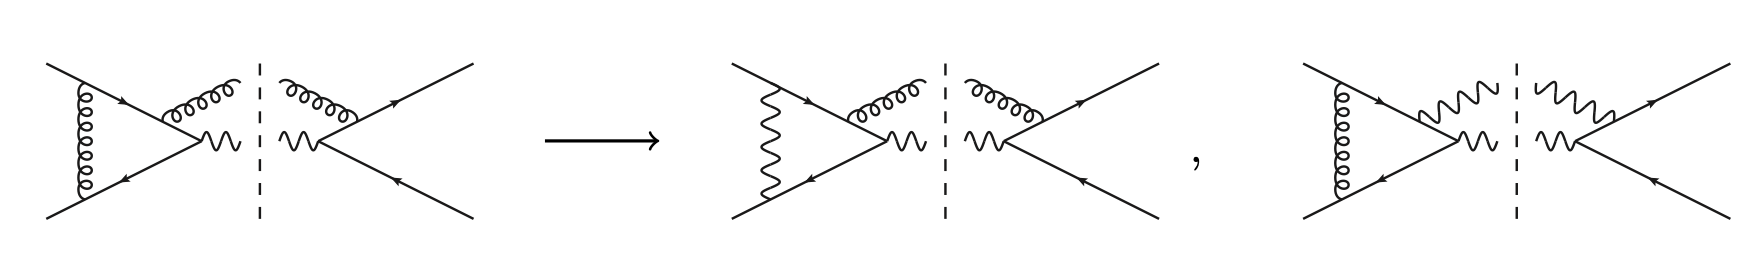
\includegraphics[width=\linewidth]{abelianization}
  \caption{Abelianization of the real-virtual correction}
  \label{fig:abel}
\end{figure}
%%%%%%%%%%%%%
To obtain the real-virtual counterterm we can exploit the {\it abelianization} of the NNLO QCD results. We based our considerations on the arguments presented in Ref. 1909.08428v1. In this paper the authors explain how the mixed QED$\times$QCD corrections can be deduce from the corresponding QCD$^2$ ones (see the Figure \ref{fig:abel}). The way to do that is by replacing
\beq
C_F^2 \; \rightarrow \; 2 C_F \, e_q^2 \, ,
\qquad 
T_R  \; \rightarrow \; 0 \, , 
\qquad 
C_A  \; \rightarrow \; 0 \, , 
\label{eq:abelianisation}
\eeq
in the QCD$^2$ results. We then report here the pure QCD result (here we are assuming to including only initial state corrections)
\beq
S_5 F_{LRV}(1,2|5) &=& 2 C_F g_{s,b}^2 \bigg[
\frac{\rho_{12}}{E_5^2 \, \rho_{15} \, \rho_{25}} \, F_{LV}(1,2)
\nn \\
&& 
- C_A [\alpha_s] \, \frac1{\epsilon^2} \, \frac{\Gamma^5(1-\epsilon) \, \Gamma^3(1+\epsilon)}{\Gamma^2(1-2\epsilon) \, \Gamma(1+2\epsilon)}
\bigg( \frac{\rho_{12}}{\rho_{15}\, \rho_{25}}\bigg)^{1+\epsilon} \, 
\frac{E_5^{-2(1+\epsilon)}}{2^{\epsilon}} F_{LM}(1,2) \; ,
\bigg]
\eeq
where 
\beq
F_{LV} (1,2) = \frac{\alpha_s}{2\pi} \, I_1(\epsilon) F_{LM}(1,2) 
+F_{LV}^{\rm fin}(1,2) \, ,
\label{eq:virtual_qcd}
\eeq
and 
\beq
I_1(\epsilon) &\equiv&
 2 {\rm Re} \Big( \mathcal{I}_1(\epsilon)\Big)
=
  2 {\rm Re} \bigg[
  \frac12 \, \frac{e^{\epsilon \gamma_E}}{\Gamma(1-\epsilon)}
  \sum_i \frac1{{\bf T}_i^2}
  \Big( {\bf T}_i^2 \, \frac1{\epsilon^2} + \gamma_i \, \frac1\epsilon \Big)
  \sum_{j\neq i} {\bf T}_i \cdot {\bf T}_j
  \Big( \frac{\mu^2 \, e^{-i \lambda_{ij} \pi}}{2p_i\cdot p_j} \Big)^\epsilon
  \bigg]
  \nn \\
 &=&
 \frac12 \, \frac{e^{\epsilon \gamma_E}}{\Gamma(1-\epsilon)} \; 
  2 {\rm Re} \bigg[  
  \Big( \frac1{\epsilon^2} + \frac{\gamma}{C_F} \, \frac1\epsilon \Big)
 {\bf T}_1 \cdot {\bf T}_2
  \Big( \frac{\mu^2 \, e^{-i \lambda_{12} \pi}}{2p_1\cdot p_2} \Big)^\epsilon
  \nn \\
  && +
  \Big(\frac1{\epsilon^2} + \frac{\gamma}{C_F}  \, \frac1\epsilon \Big)
   {\bf T}_2 \cdot {\bf T}_1
  \Big( \frac{\mu^2 \, e^{-i \lambda_{21} \pi}}{2p_2\cdot p_1} \Big)^\epsilon
  \bigg]
  \nn \\
 &=&-2C_F
 \frac12 \, \frac{e^{\epsilon \gamma_E}}{\Gamma(1-\epsilon)} \; 
 \Big( \frac1{\epsilon^2} + \frac32 \, \frac1\epsilon \Big) \; 
  \Big( \frac{\mu^2 }{s_{12}} \Big)^\epsilon \; 
  2 {\rm Re}    
  \Big( e^{-i \pi \epsilon}\Big)
   \nn \\
 &=&-2C_F \, 
\frac{e^{\epsilon \gamma_E}}{\Gamma(1-\epsilon)} \; 
 \Big( \frac1{\epsilon^2} + \frac32 \, \frac1\epsilon \Big) \; 
  \Big( \frac{\mu^2 }{s_{12}} \Big)^\epsilon \; 
 \cos( \pi \epsilon)
 \label{eq:soft_virtual_current_qcd}
\eeq
$\gamma_1 = \gamma_{2} = \gamma = \frac32 C_F, {\bf T}_1^2={\bf T}_2^2=C_F$, $ {\bf T}_1=- {\bf T}_2$, $\lambda_{12}=\lambda_{21}=1$.
Putting all the ingredients together we obtain
\beq
S_5 F_{LRV}(1,2|5) &=& 2 C_F g_{s,b}^2 \bigg[
\frac{\rho_{12}}{E_5^2 \, \rho_{15} \, \rho_{25}} \, 
\Big[-2C_F \, \frac{\alpha_s}{2\pi}
\frac{e^{\epsilon \gamma_E}}{\Gamma(1-\epsilon)} \; 
 \Big( \frac1{\epsilon^2} + \frac32 \, \frac1\epsilon \Big) \; 
  \Big( \frac{\mu^2 }{s_{12}} \Big)^\epsilon \; 
 \cos( \pi \epsilon)
 \nn \\
 && \hspace{40mm}
 +F_{LV}^{\rm fin}(1,2)
 \Big]
\nn \\
&& 
- C_A [\alpha_s] \, \frac1{\epsilon^2} \, \frac{\Gamma^5(1-\epsilon) \, \Gamma^3(1+\epsilon)}{\Gamma^2(1-2\epsilon) \, \Gamma(1+2\epsilon)}
\bigg( \frac{\rho_{12}}{\rho_{15}\, \rho_{25}}\bigg)^{1+\epsilon} \, 
\frac{E_5^{-2(1+\epsilon)}}{2^{\epsilon}} F_{LM}(1,2) \; ,
\bigg] \, .
\nn \\
&=& 2 C_F \,
8 \pi^2 \, [\alpha_s] \,
\frac{\Gamma(1-\epsilon)}{(4\pi)^\epsilon} \, 
\bigg[
\frac{\rho_{12}}{E_5^2 \, \rho_{15} \, \rho_{25}} \, 
\Big[-2C_F \,
[\alpha_s] \, 
 \Big( \frac1{\epsilon^2} + \frac32 \, \frac1\epsilon \Big) \; 
s_{12}^{-\epsilon} \; 
 \cos( \pi \epsilon)
  \nn \\
 && \hspace{60mm}
 +F_{LV}^{\rm fin}(1,2)
 \Big]
\nn \\
&& 
- C_A [\alpha_s] \, \frac1{\epsilon^2} \, \frac{\Gamma^5(1-\epsilon) \, \Gamma^3(1+\epsilon)}{\Gamma^2(1-2\epsilon) \, \Gamma(1+2\epsilon)}
\bigg( \frac{\rho_{12}}{\rho_{15}\, \rho_{25}}\bigg)^{1+\epsilon} \, 
\frac{E_5^{-2(1+\epsilon)}}{2^{\epsilon}} F_{LM}(1,2) \; ,
\bigg] \, .
\eeq
Applying the substitutions listed in Eq.\eqref{eq:abelianisation} we get
\beq
S_5 F_{LRV}(1,2|5) 
&=& 
- 4 \cdot 2 C_F \, Q_f^2 \;
8 \pi^2 \, [\alpha_s]\, [\alpha] \,
\frac{\Gamma(1-\epsilon)}{(4\pi)^\epsilon} \, 
\frac{\rho_{12}}{E_5^2 \, \rho_{15} \, \rho_{25}} \, 
 \Big( \frac1{\epsilon^2} + \frac32 \, \frac1\epsilon \Big) \; 
s_{12}^{-\epsilon} \; 
 \cos( \pi \epsilon) \, .
 \nn \\
 &&
 +
 2 C_F \,
8 \pi^2 \, [\alpha_s] \,
\frac{\Gamma(1-\epsilon)}{(4\pi)^\epsilon} \, 
\frac{\rho_{12}}{E_5^2 \, \rho_{15} \, \rho_{25}} \, 
F_{LV}^{\rm fin}(1,2)\Big|_{C_F \rightarrow 2 Q_f^2, \, \alpha_s \rightarrow \alpha}
 \eeq
The fundamental structure to integrate is again of the type presented in Eq.\eqref{eq:single-soft_int}, and therefore we have
\beq
\langle S_5 F_{LRV}(1,2|5)  \rangle
&=&
- 8 C_F \, Q_f^2 \;
[\alpha_s] \, [\alpha] \, 
\frac{1}{\eps^2} (4 E_{\rm max})^{-\eps} \, 
\frac{\Gamma^2(1-\eps)}{\Gamma(1-2\eps)} \, 
s_{12}^{-\epsilon} \, K_{12}\, 
 \Big( \frac1{\epsilon^2} + \frac32 \, \frac1\epsilon \Big) \,
 \cos( \pi \epsilon)  
 \nn \\
 &&
 +
 2 C_F \,
[\alpha_s] \,
\frac{1}{\eps^2} (4 E_{\rm max})^{-\eps} 
\frac{\Gamma^2(1-\eps)}{\Gamma(1-2\eps)} \, K_{12} \, 
F_{LV}^{\rm fin}(1,2)\Big|_{C_F \rightarrow 2 Q_f^2, \, \alpha_s \rightarrow \alpha}\, .
\eeq
Two main problems have still to be solved
\begin{itemize}
\item include photon-lepton interactions, 
\item include renormalisation.
\end{itemize}
To address the first requirement we consider the factorised contribution of a QCD radiation times a QED virtual correction and {\it viceversa}. In formulae
\beq
S_5 F_{LRV}(1,2|5) &=& 2 C_F g_{s,b}^2 \; 
\mathcal{S}_{12} (p_5) \, F_{LV}^\gamma(1,2)
\nn \\
&& 
{\color{red}{+}} 2 g_{b}^2 \Big[ 
 Q_f^2 \, \mathcal{S}_{12} (p_5)
 - Q_f \, \mathcal{S}_{13} (p_5)
 + Q_f \, \mathcal{S}_{14} (p_5)
 + Q_f \, \mathcal{S}_{23} (p_5)
 \nn \\
 && \hspace{15mm}
 - Q_f \, \mathcal{S}_{24} (p_5)
 + \mathcal{S}_{34} (p_5)
 \Big] \, F_{LV}^g(1,2)
 \eeq
 where the QED virtual correction has been discussed in Eq.\eqref{eq:qed_virtual}, and the QCD virtual correction is Eqs.\eqref{eq:virtual_qcd}-\eqref{eq:soft_virtual_current_qcd}
\beq
F_{LV} ^g(1,2) &=&
 \frac{\alpha_s}{2\pi} \, I^g_1(\epsilon) F_{LM}(1,2) 
+F_{LV}^{g, \, \rm fin}(1,2) 
\nn \\
&=& 
\frac{\alpha_s}{2\pi}
(-2C_F) \, 
\frac{e^{\epsilon \gamma_E}}{\Gamma(1-\epsilon)} \; 
 \Big( \frac1{\epsilon^2} + \frac32 \, \frac1\epsilon \Big) \; 
  \Big( \frac{\mu^2 }{s_{12}} \Big)^\epsilon \; 
 \cos( \pi \epsilon)  F_{LM}(1,2) 
 +F_{LV}^{g, \, \rm fin}(1,2) 
 \nn \\
F_{LV}^\gamma (1,2) &=& \frac{\alpha}{2\pi} \, I^\gamma_1(\epsilon) F_{LM}(1,2) 
+F_{LV}^{\gamma, \, \rm fin}(1,2)
\nn \\
&=& 
{\color{red}{-}}
\frac{\alpha}{2\pi} \, 
 \frac{e^{\eps \gamma_E}}{\Gamma(1-\eps)}
\Big( \frac1{\eps^2}+\frac32 \frac1\eps 
\Big) \; 
2 {\rm Re}
\bigg[
Q_f^2 \bigg(\frac{\mu^2 \, e^{-i \pi}}{s_{12}}\bigg)^\eps
+  \bigg(\frac{\mu^2 \, e^{-i \pi}}{s_{34}}\bigg)^\eps
- Q_f \bigg(\frac{\mu^2}{s_{13}}\bigg)^\eps
\nn \\
&& 
\hspace{15mm}
+ Q_f \bigg(\frac{\mu^2}{s_{14}}\bigg)^\eps
+ Q_f \bigg(\frac{\mu^2}{s_{23}}\bigg)^\eps
- Q_f \bigg(\frac{\mu^2}{s_{24}}\bigg)^\eps
\bigg] F_{LM}(1,2) 
+F_{LV}^{\gamma, \, \rm fin}(1,2)
\nn \\
&=& 
{\color{red}{-}}
\frac{\alpha}{2\pi} \, 
 \frac{e^{\eps \gamma_E}}{\Gamma(1-\eps)}
\Big( \frac1{\eps^2}+\frac32 \frac1\eps 
\Big) \; 
2 \, 
\bigg[
Q_f^2 \bigg(\frac{\mu^2 }{s_{12}}\bigg)^\eps \cos(\pi \epsilon)
+  \bigg(\frac{\mu^2 }{s_{34}}\bigg)^\eps \cos(\pi \epsilon)
- Q_f \bigg(\frac{\mu^2}{s_{13}}\bigg)^\eps
\nn \\
&& 
\hspace{15mm}
+ Q_f \bigg(\frac{\mu^2}{s_{14}}\bigg)^\eps
+ Q_f \bigg(\frac{\mu^2}{s_{23}}\bigg)^\eps
- Q_f \bigg(\frac{\mu^2}{s_{24}}\bigg)^\eps
\bigg] F_{LM}(1,2) 
+F_{LV}^{\gamma, \, \rm fin}(1,2)
\eeq
The soft-real-virtual counterterm is then given by
\beq
S_5 F_{LRV}(1,2|5) &=& 
{\color{red}{-}}
2 C_F g_{s,b}^2 \; 
\mathcal{S}_{12} (p_5) \, \bigg\{
\frac{\alpha}{2\pi} \, 
 \frac{e^{\eps \gamma_E}}{\Gamma(1-\eps)}
\Big( \frac1{\eps^2}+\frac32 \frac1\eps 
\Big) \; 
2 \, 
\bigg[
Q_f^2 \bigg(\frac{\mu^2 }{s_{12}}\bigg)^\eps \cos(\pi \epsilon)
\nn \\
&& \qquad 
+  \bigg(\frac{\mu^2 }{s_{34}}\bigg)^\eps \cos(\pi \epsilon)
- Q_f \bigg(\frac{\mu^2}{s_{13}}\bigg)^\eps
+ Q_f \bigg(\frac{\mu^2}{s_{14}}\bigg)^\eps
+ Q_f \bigg(\frac{\mu^2}{s_{23}}\bigg)^\eps
\nn \\
&& \qquad
- Q_f \bigg(\frac{\mu^2}{s_{24}}\bigg)^\eps
\bigg] F_{LM}(1,2) 
+F_{LV}^{\gamma, \, \rm fin}(1,2)
\bigg\}
\nn \\
&& 
{\color{red}{+}} 2 g_{b}^2 \Big[ 
 Q_f^2 \, \mathcal{S}_{12} (p_5)
 - Q_f \, \mathcal{S}_{13} (p_5)
 + Q_f \, \mathcal{S}_{14} (p_5)
 + Q_f \, \mathcal{S}_{23} (p_5)
 - Q_f \, \mathcal{S}_{24} (p_5)
 \nn \\
 && \qquad 
 + \mathcal{S}_{34} (p_5)
 \Big] \, \bigg\{
 \frac{\alpha_s}{2\pi}
(-2C_F) \, 
\frac{e^{\epsilon \gamma_E}}{\Gamma(1-\epsilon)} \; 
 \Big( \frac1{\epsilon^2} + \frac32 \, \frac1\epsilon \Big) \; 
  \Big( \frac{\mu^2 }{s_{12}} \Big)^\epsilon \; 
 \cos( \pi \epsilon)  F_{LM}(1,2) 
 \nn \\
 && \qquad 
 +F_{LV}^{g, \, \rm fin}(1,2)
 \bigg\} \; .
 \eeq
The integration over the unresolved real-radiation phase space returns 
\beq
\langle 
S_5 F_{LRV}(1,2|5) \rangle
 &=& 
{\color{red}{-}} 2 C_F g_{s,b}^2 \; 
\frac{1}{\eps^2} (4 E_{\rm max})^{-\eps} 
\frac{1}{8\pi^2} \frac{(4\pi)^\eps}{\Gamma(1-\eps)}
\frac{\Gamma^2(1-\eps)}{\Gamma(1-2\eps)} \, K_{12} \times
\nn \\
&& \times 
 \, \bigg\{
\frac{\alpha}{2\pi} \, 
 \frac{e^{\eps \gamma_E}}{\Gamma(1-\eps)}
\Big( \frac1{\eps^2}+\frac32 \frac1\eps 
\Big) \; 
2 \, 
\bigg[
Q_f^2 \bigg(\frac{\mu^2 }{s_{12}}\bigg)^\eps \cos(\pi \epsilon)
\nn \\
&& \qquad 
+  \bigg(\frac{\mu^2 }{s_{34}}\bigg)^\eps \cos(\pi \epsilon)
- Q_f \bigg(\frac{\mu^2}{s_{13}}\bigg)^\eps
+ Q_f \bigg(\frac{\mu^2}{s_{14}}\bigg)^\eps
+ Q_f \bigg(\frac{\mu^2}{s_{23}}\bigg)^\eps
\nn \\
&& \qquad
- Q_f \bigg(\frac{\mu^2}{s_{24}}\bigg)^\eps
\bigg] F_{LM}(1,2) 
+F_{LV}^{\gamma, \, \rm fin}(1,2)
\bigg\}
\nn \\
&& 
{\color{red}{+}} 2 g_{b}^2 \,\frac{1}{\eps^2} (4 E_{\rm max})^{-\eps} \frac{1}{8\pi^2} \frac{(4\pi)^\eps}{\Gamma(1-\eps)}
\frac{\Gamma^2(1-\eps)}{\Gamma(1-2\eps)}
\Big[ 
 Q_f^2  \, K_{12}
 - Q_f  \, K_{13}
\nn \\
&&
 + Q_f \, K_{14}
 + Q_f \, K_{23}
 - Q_f \, K_{24}
 +  \, K_{34}
 \Big] \, \bigg\{
 \frac{\alpha_s}{2\pi}
(-2C_F) \, 
\frac{e^{\epsilon \gamma_E}}{\Gamma(1-\epsilon)} \; \times
\nn \\
&& \times
 \Big( \frac1{\epsilon^2} + \frac32 \, \frac1\epsilon \Big) \; 
  \Big( \frac{\mu^2 }{s_{12}} \Big)^\epsilon \; 
 \cos( \pi \epsilon)  F_{LM}(1,2) 
 +F_{LV}^{g, \, \rm fin}(1,2)
 \bigg\} 
 \nn \\
 &=& 
{\color{red}{-}} 4 C_F [\alpha_s] \; 
\frac{1}{\eps^2} (4 E_{\rm max})^{-\eps} 
\frac{\Gamma^2(1-\eps)}{\Gamma(1-2\eps)} \, K_{12} \, 
\bigg\{
[\alpha]
\Big( \frac1{\eps^2}+\frac32 \frac1\eps 
\Big) \; 
\bigg[
Q_f^2 \, s_{12}^{-\eps} \cos(\pi \epsilon)
\nn \\
&& \qquad 
+  \,s_{34}^{-\eps} \cos(\pi \epsilon)
- Q_f \, s_{13}^{-\eps}
+ Q_f \, s_{14}^{-\eps}
+ Q_f \, s_{23}^{-\eps}
- Q_f \, s_{24}^{-\eps}
\bigg] F_{LM}(1,2) 
\nn \\
&& \qquad 
+F_{LV}^{\gamma, \, \rm fin}(1,2)
\bigg\}
\nn \\
&& 
{\color{red}{+}} 2 [\alpha]
 \,\frac{1}{\eps^2} (4 E_{\rm max})^{-\eps} \, 
\frac{\Gamma^2(1-\eps)}{\Gamma(1-2\eps)}
\Big[ 
 Q_f^2  \, K_{12}
 - Q_f  \, K_{13}
 + Q_f \, K_{14}
 + Q_f \, K_{23}
\nn \\
&&
 - Q_f \, K_{24}
 +  \, K_{34}
 \Big] \, \bigg\{
 [\alpha_s]
(-2C_F) \, 
 \Big( \frac1{\epsilon^2} + \frac32 \, \frac1\epsilon \Big) \; 
  s_{12}^{-\epsilon} \; 
 \cos( \pi \epsilon)  F_{LM}(1,2) 
 \nn \\
 && \qquad 
 +F_{LV}^{g, \, \rm fin}(1,2)
 \bigg\} 
 \; .
 \eeq
 Assuming to neglect the contribution of the lepton we would have
 \beq
\langle S_5 F_{LRV}(1,2|5) \rangle 
 \!\!\!&=& \!\!\!
{\color{red}{-}} 4 C_F [\alpha_s] \; 
\frac{1}{\eps^2} (4 E_{\rm max})^{-\eps} 
\frac{\Gamma^2(1-\eps)}{\Gamma(1-2\eps)} \, K_{12} \, 
\bigg\{
[\alpha]
\Big( \frac1{\eps^2}+\frac32 \frac1\eps 
\Big) \,
Q_f^2 \, s_{12}^{-\eps} \cos(\pi \epsilon) F_{LM}(1,2) 
\nn \\
&& \qquad 
+F_{LV}^{\gamma, \, \rm fin}(1,2)
\bigg\}
\nn \\
&& 
{\color{red}{-}} 2 [\alpha]
 \,\frac{1}{\eps^2} (4 E_{\rm max})^{-\eps} \, 
\frac{\Gamma^2(1-\eps)}{\Gamma(1-2\eps)} \, 
 Q_f^2  \, K_{12}\, \bigg\{
 2C_F
 [\alpha_s]
 \Big( \frac1{\epsilon^2} + \frac32 \, \frac1\epsilon \Big) \; 
  s_{12}^{-\epsilon} \,
 \cos( \pi \epsilon)  F_{LM}(1,2) 
 \nn \\
 && \qquad 
 -F_{LV}^{g, \, \rm fin}(1,2)
 \bigg\} 
 \; ,
 \eeq
 which is in agreement with the result obtained {\it via} abelianization.

\end{document}